% ------------------------------------------------------------------------
% ------------------------------------------------------------------------
% ICMC: Modelo de Trabalho Acadêmico (tese de doutorado, dissertação de
% mestrado e trabalhos monográficos em geral) em conformidade com 
% ABNT NBR 14724:2011: Informação e documentação - Trabalhos acadêmicos -
% Apresentação
% ------------------------------------------------------------------------
% ------------------------------------------------------------------------

% Opções: 
%   Qualificação          = qualificacao 
%   Curso                 = doutorado/mestrado
%   Situação do trabalho  = pre-defesa/pos-defesa (exceto para qualificação)
%   Versão para impressão = impressao
\documentclass[doutorado, pre-defesa]{packages/icmc}

% ---------------------------------------------------------------------------
% Pacotes Opcionais
% ---------------------------------------------------------------------------
\usepackage{rotating}           % Usado para rotacionar o texto
\usepackage[all,knot,arc,import,poly]{xy}   % Pacote para desenhos gráficos
% Este pacote pode conflitar com outros pacotes gráficos como o ``pictex''
% Então é necessário usar apenas um dos pacotes conflitantes
\newcommand{\VerbL}{0.52\textwidth}
\newcommand{\LatL}{0.42\textwidth}

\usepackage{multirow} % multirow
\usepackage{lscape}
\usepackage{graphicx}
\usepackage{soul}
% ---------------------------------------------------------------------------
\algnewcommand{\LeftComment}[1]{\Statex \(\triangleright\) #1}

\newcolumntype{L}[1]{>{\raggedright\arraybackslash}p{#1}}
\newcolumntype{C}[1]{>{\centering\arraybackslash}p{#1}}
\newcolumntype{R}[1]{>{\raggedleft\arraybackslash}p{#1}}
% ---
% Informações de dados para CAPA e FOLHA DE ROSTO
% ---
% Tanto na capa quanto nas folhas de rosto apenas a primeira letra da primeira palavra (ou nomes próprios) devem estar em letra maiúscula, todas as demais devem ser em letra minúscula.
\tituloEN{Gamification of Collaborative Learning Scenarios: An Ontological Engineering Approach to Deal with the Motivation Problem Caused by Computer-Supported Collaborative Learning Scripts}
\tituloPT{Gamificação de Cenários de Aprendizagem Colaborativa: Uma Abordagem de Engenharia de Ontologias para Lidar com o Problema de Motivação Causado por Scripts de Aprendizagem Colaborativa Suportados por Computador}

\autor[Challco, G. C.]{Geiser Chalco Challco}
\genero{M} % Gênero do autor (M = Masculino / F = Feminino)
\orientador[Orientadora]{Prof. Dr.}{Seiji Isotani}%\coorientador{Prof. Dr.}{Fulano de Tal}
\curso{CCMC}
\data{07}{07}{2018} % Data do depósito
\idioma{EN} % Idioma principal do documento (PT = português / EN = inglês)
% ---


% ---
% RESUMOS
% ---

% resumo em INGLÊS
% conter no máximo 500 palavras
% conter no mínimo 1 e no máximo 5 palavras-chave
%\textoresumo[english]{
%    Content}{Word1, Word2, Word3, Word4, Word5}

% Resumo em PORTUGUÊS
% conter no máximo 500 palavras
% conter no mínimo 1 e no máximo 5 palavras-chave
%\textoresumo[brazil]{
%    Conteúdo}{Word1, Word2, Word3, Word4, Word5, Word6}



% ----------------------------------------------------------
% ELEMENTOS PRÉ-TEXTUAIS
% ----------------------------------------------------------

% Inserir a ficha catalográfica
%\incluifichacatalografica{tex/pre-textual/ficha-catalografica.pdf}

% DEDICATÓRIA / AGRADECIMENTO / EPÍGRAFE
%\textodedicatoria*{tex/pre-textual/dedicatoria}
%\textoagradecimentos*{tex/pre-textual/agradecimentos}
%\textoepigrafe*{tex/pre-textual/epigrafe}

% Inclui a lista de figuras
%\incluilistadefiguras

% Inclui a lista de tabelas
%\incluilistadetabelas

% Inclui a lista de quadros
%\incluilistadequadros

% Inclui a lista de algoritmos
%\incluilistadealgoritmos

% Inclui a lista de códigos
%\incluilistadecodigos

% Inclui a lista de siglas e abreviaturas
%\incluilistadesiglas

% Inclui a lista de símbolos
%\incluilistadesimbolos

% ----
% Início do documento
% ----
\begin{document}
% ----------------------------------------------------------
% ELEMENTOS TEXTUAIS
% ----------------------------------------------------------
\textual

\newcommand{\comando}[1]{\textbf{$\backslash$#1}}


\chapter{Introduction}
\label{chapter:introducao}

This chapter starts with the context and delimitation of research problem (\autoref{sec:problem-delimitation}). After that, the chapter formulates the research questions and objectives (\autoref{sec:research-question-and-research-objectives}).
The research methodology is presented in \autoref{sec:research-methodology}.
The thesis statement and contributions are detailed in \autoref{sec:thesis-statement-and-claimed-contributions}. Finally, the chapter ends with the structure of this dissertation (\autoref{sec:structure-of-dissertation}).

\section{Context and Problem Delimitation}
\label{sec:problem-delimitation}

Over the last two decades or so, with the growing number of technologies that enable people to communicate and work in group activities using computers and Internet, researches and practitioners have developed technology and software applications that facilitate and foster the Collaborative Learning (CL) \cite{LehtinenHakkarainenLipponenRahikainenMuukkonen1999}.
The research field that studies how this technology should link the advanced in computer science with the pedagogical approaches of collaborative learning is known as Computer-Supported Collaborative Learning (CSCL), and it has been proved an important research field to support the learning process of students \cite{StahlKoschmannSuthers2006}.
Some of the most relevant benefits of the integration between computer sciences and collaborative learning are: to facilitate the sharing and distribution of knowledge among group members \cite{Lipponen2002,NordinKlobas2010},
to help the monitoring and evaluation of CL process \cite{Rodriguez-TrianaPrietoMartinez-MonesAsensio-PerezDimitriadis2018,CaballeDaradoumisXhafaJuan2011},
and to enhance the peer interactions and work in groups \cite{Wang2014,ZhaoGaoYang2018}.

The benefits of a CSCL technology are better obtained by the students when there is an adequate design of the CL process, when there is a support to orchestrate and to indicate in which way the students should collaborate to achieve pedagogical benefits \cite{Dillenbourg2013, Hewitt2005, IsotaniInabaIkedaMizoguchi2009}.
When there is not such support, students frequently fail to act or behave in a productive way.
In a CL session, the participants need to know with whom they must work,
they need to known what are their roles in the CL process, and
they need to known what are the steps that must be done to accomplish their learning goals.
Without this information, frequently, the participants will not adequately collaborate or leave to interact during the CL activities.
Hence, several researchers propose the use of scripts to guide and orchestrate the collaboration in these activities \cite{AlharbiAthaudaChiong2014}.

The scripted collaboration aims to engage the students in fruitful and meaningful interactions according to a design that has the purpose to attain a set of pedagogical objectives.
Thereby, CSCL scripts have been proposed by the community to support the well-thought-out design of the CL scenarios by means of computer-based systems \cite{FischerKollarStegmannWeckerZottmann2013,KobbeWeinbergerDillenbourgHarrerHamalainenHakkinenFischer2007}.
These scripts are the technology that describes how the interactions among students will be orchestrated in a group activity to increase the possibility of achieving the pedagogical objectives \cite{WeinbergerErtlFischerMandl2005}. These scripts provide information that facilitates the group formation, the role distribution, and the sequencing of interaction for the participants in the CL process.
Despite of its benefits, there are situations in which the scripts may cause motivational problems.
For example, when the students prefers to work individually or when they does not want to play the role assigned by the scripts, they may neglect their personal behavior to get the task completed without effort, and the lack of choice over the interactions may produce in them a sense of obligation.
These issues degrade the group dynamic (e.g. some students may dropout the CL activity, making superficial interactions) resulting in negative and widespread learning outcomes.

The motivational problems in the scripted collaboration make more difficult the use of this technology over time.
In fact, less motivated students prefer to spend more time in other activities rather than to collaboratively learn and, as consequence, the achievement of expected learning outcomes becomes more difficult \cite{Crook2000, FaloutElwoodHood2009, SchoorBannert2011}.
In this sense, motivating learners in the entire CL process is important.
However, the traditional instructional design practice often assumes that the motivation is a preliminary step that occurs outside to the learning process \cite{ChanAhern1999, Keller1987}.
This assumption is based in which the good quality of learning materials and content-domain can keep the students focused during the learning process, but if this process is long, there is a good chance that the students will lose their initial motivation.
To avoid this motivational problem known as demotivation, the development and use of affective feedback systems based on emotion-aware systems \cite{FeidakisDaradoumisCaballeConesa2014,FeidakisCaballeDaradoumisJimenezConesa2014}, and learning companions \cite{WoolfBurlesonArroyoDragonCooperPicard2009}, have been proposed to motivated students along the entire learning process.
These solutions assume that the students like the content-domain and that they have the desired to learn working in groups, so that students that do not have the desire to learn or do not want to work in groups are not motivated and engaged for the approach of using affective feedback systems.

In the last years, efforts of CSCL community have been directed to finding new innovative solutions that, beside to motivate and engage students during the entire CL process, are not completely tied to the domain-content and desired to learn working in groups.
In this direction, several researchers and practitioners have pointed Gamification as a promising technology to deal with motivational problems in educational contexts \cite{ChallcoMoreiraMizoguchiIsotani2014, SeabornFels2015, BorgesDurelliReisIsotani2014}.
Gamification \aspas{\emph{as the use of game design elements in non-game contexts}} \cite{DeterdingDixonKhaledNacke2011} aims to increase the students' motivation and engagement by making the learning process more game-like.
Through the introduction of game elements, such as points, leaderboards, competition, cooperation and so on, gamification intends to engage and motivate students who do not have the desire or interest in to learn the content-domain working in groups.
According to \cite{Kapp2012, KnutasIkonenNikulaPorras2014}, when a learning process is gamified, the benefits of introduced game elements will strongly depend on how well these game elements will be applied, and how well they are linked with the pedagogical approaches employed in the learning process.

When CL scenarios are gamified to deal with the motivational problems that can occur in the scripted collaboration, the author of this thesis hypothesizes that the chances to achieve engagement and educational benefits will be increased whether there is a proper connection between the game elements and the CL process.
Nevertheless, developing such well-though-out gamified CL scenario, hereinafter referred to as gamified CL scenarios, is a non-trivial task.
The main difficulty to gamify CL scenarios as well as other non-game context is that the gamification is too context dependent \cite{HamariKoivistoSarsa2014, RichardsThompsonGraham2014}.
Its effects vary from individual to individual, from situation to situation, and from time to time.
Gamification depends of many factors such as the individual personality traits, preferences, and current student's emotions \cite{Nicholson2015, PedroLopesPratesVassilevaIsotani2015}
(e.g., a leaderboard would motivate users who like competition but not users who desire to obtain items to customize their avatars).
Also, the expected effects of the game elements vary according to the non-game context and the target behavior that is being gamified \cite{DeterdingBjorkNackeDixonLawley2013, HeeterLeeMedlerMagerko2011}
(e.g., gamifying a learning scenario to promote the signing-up is not the same thing as gamifying an interactive environment to maintain the students attention).
As consequence of this context-dependency, when a CL scenario is not well gamified, instead to have a positive effect, they may cause a detrimental on the students' motivation \cite{AndradeMizoguchiIsotani2016}, cheating \cite{NunesBittencourtIsotaniJaques2016}, embarrassment \cite{OhnoYamasakiTokiwa2013}, and lack of credibility on badges \cite{DavisSingh2015}.

Another difficulty to gamify CL scenarios, as well as other non-game contexts, it is the lack of approaches to systematically represent, in an unambiguous way, the gamification knowledge acquired in the last years by researchers and practitioners.
This knowledge constituted by theories and practices related to gamification lacks of a formal and common vocabulary, definitions, and representation to apply gamification.
As can be appreciated in the current literature of gamification \cite{DichevaDichevAgreAngelova2015, HamariKoivistoSarsa2014, MoraRieraGonzalezArnedo-Moreno2015, SeabornFels2015}, each author proposes his/her own definitions, classifications and representations of concepts and characteristics about how to gamify a non-game context. This fact hinders the creation of models/frameworks that formally represent the gamification and its application in a common understandable and shareable manner.
To the best of the thesis author's knowledge, there is no one approach to represent the knowledge about how to gamify CL scenarios, and how through the gamification is possible to deal with motivational problems in the scripted collaboration.

Due to the variety of students who can participate in CL sessions, the diversity of subjects that can be under study in a CL activity, and the range of different CSCL scripts that can be used to orchestrate the CL process, it is necessary to personalize the gamification for each student and situation, so providing a tailored gamified CL scenario is necessary to obtain better benefits of gamification.
Developing tailored gamified CL scenarios is a difficult and time-consuming task, so that a computational based-support to give assistance for personalizing gamification is necessary and very helpful.
In this direction, in the context of CSCL, there is only one interesting approach that proposes to personalize gamification based on individual preference profiles obtained from interaction analysis by machine learning techniques \cite{KnutasvanRoyHynninenGranatoKasurinenIkonen2017,KnutasIkonenMaggioriniRipamontiPorras2016,KnutasIkonenNikulaPorras2014}.
However, this solution is not oriented to deal with motivational problems in the scripted collaboration, its purpose is to increase the communication among the participants in a CL scenarios (not necessarily scripted).
Furthermore, this solution does not provide a model to share the theoretical knowledge related to gamification obtained by its computer-based mechanism to personalize the gamification.
Solutions based on machine learning to personalize gamification require a lot of data to support the personalization of gamification, and they may fall in an overfitting or underfitting problem with the data.
A computational mechanism based only in machine learning techniques to personalize gamification will always lack of theoretical-justification to explain why a game element is introduced, and why a certain configuration of game elements engage and motivate the participants to continue and adequadely interact in the CL scenario.

For the reason exposed above, to deal with motivational problems in the scripted collaboration through the gamification, a computational support with common and shareable structures to describe the knowledge extracted from the practices and theories related to gamification is essential to overcome the challenges and difficulties of gamification.
In the direction to make explicit the knowledge contained in computational mechanisms and procedures, ontologies have been consolidated as the most advanced technology to support the representation of knowledge in a common understandable and shareable manner for computers and humans \cite{AsikriLaassiriKritChaib2016, Devedzic2006, MizoguchiBourdeau2016}.
Ontologies constitute an explicit mapping between the target world of interest and its representation with the purpose to describe concepts without ambiguities providing a common way to represent the knowledge \cite{GuarinoOberleStaab2009}.
Taking advantages of this commonality and using the computer interconnection provided by Internet, computational mechanisms and procedures for intelligent tools can be developed to use the ontologies as a language to share the understandings and interpretations of \emph{target world} - in this thesis dissertation, the target world is the gamification of CL scenario.

Employing ontologies, some interesting and practical results have been obtained to formalize and to organize the knowledge extracted from different theories and practices related to gamification \cite{DermevalVilelaBittencourtCastroIsotaniBritoSilva2016, KarkarAlJa'amFoufou2016, ZouaqNkambou2010}.
However, currently, to the best of the thesis author knowledge, there is no one ontology that allows to describe the theoretical foundation extracted from the practices and theories related to gamification, and how these concepts are applied in CL scenarios to deal with motivational problems in the scripted collaboration.
Therefore, the general research goal in this thesis dissertation refers to the definition of an ontology to systematically formalize the knowledge extracted from the practices and theories related to gamification from a philosophical perspective.
This ontology has also been developed by the thesis author to give support in intelligent tools that employ the ontological structures in their computational mechanisms and procedures to deal with motivational problems in  the \emph{scripted collaboration} -
by the scripted collaboration, the thesis author specifically refers to CL activities where the CSCL scripts are used as a method to orchestrate and structure the collaboration among students.

\section{Research Questions and Research Objectives}
\label{sec:research-question-and-research-objectives}

The research topic explored in this PhD thesis dissertation is addressed to answer the question:
\aspas{\emph{How to deal with motivational problems in the scripted collaboration?}}

To answer this research question, the author of this thesis proposes the gamification of CL scenarios.
However, as was explained in the previous section, gamification is too context dependent, so that, to obtain tailored gamified CL scenarios, intelligent tools are necessary to give support in the personalization of gamification. 
In this sense, it is necessary a common way to represent the knowledge extracted from practices and theories related to gamification because an adequate gamification of CL scenarios should rely on this theoretical knowledge.
Thus, the use of ontologies is proposed by the thesis author to represent this knowledge because ontologies have been consolidated as the technology in which computers and humans use a common language to build models/frameworks about the target world that is being represented. 
Thereby, the overaching research question (\textbf{RQ}) addressed in this thesis is: 

\aspas{\emph{How can gamification and ontologies be used to deal with motivational problems in the scripted collaboration?}}

To answer this research question, the ontological engineering approach to gamify CL scenarios shown in \autoref{fig:ontological-engineering-approach-to-gamify-cl-scenarios} has been proposed by the author of this PhD thesis dissertation. 
This approach consists into three major stages described as follows:

\begin{figure}[htb]
 \caption{Ontological engineering approach to gamify CL scenarios}
 \label{fig:ontological-engineering-approach-to-gamify-cl-scenarios}
 \centering
 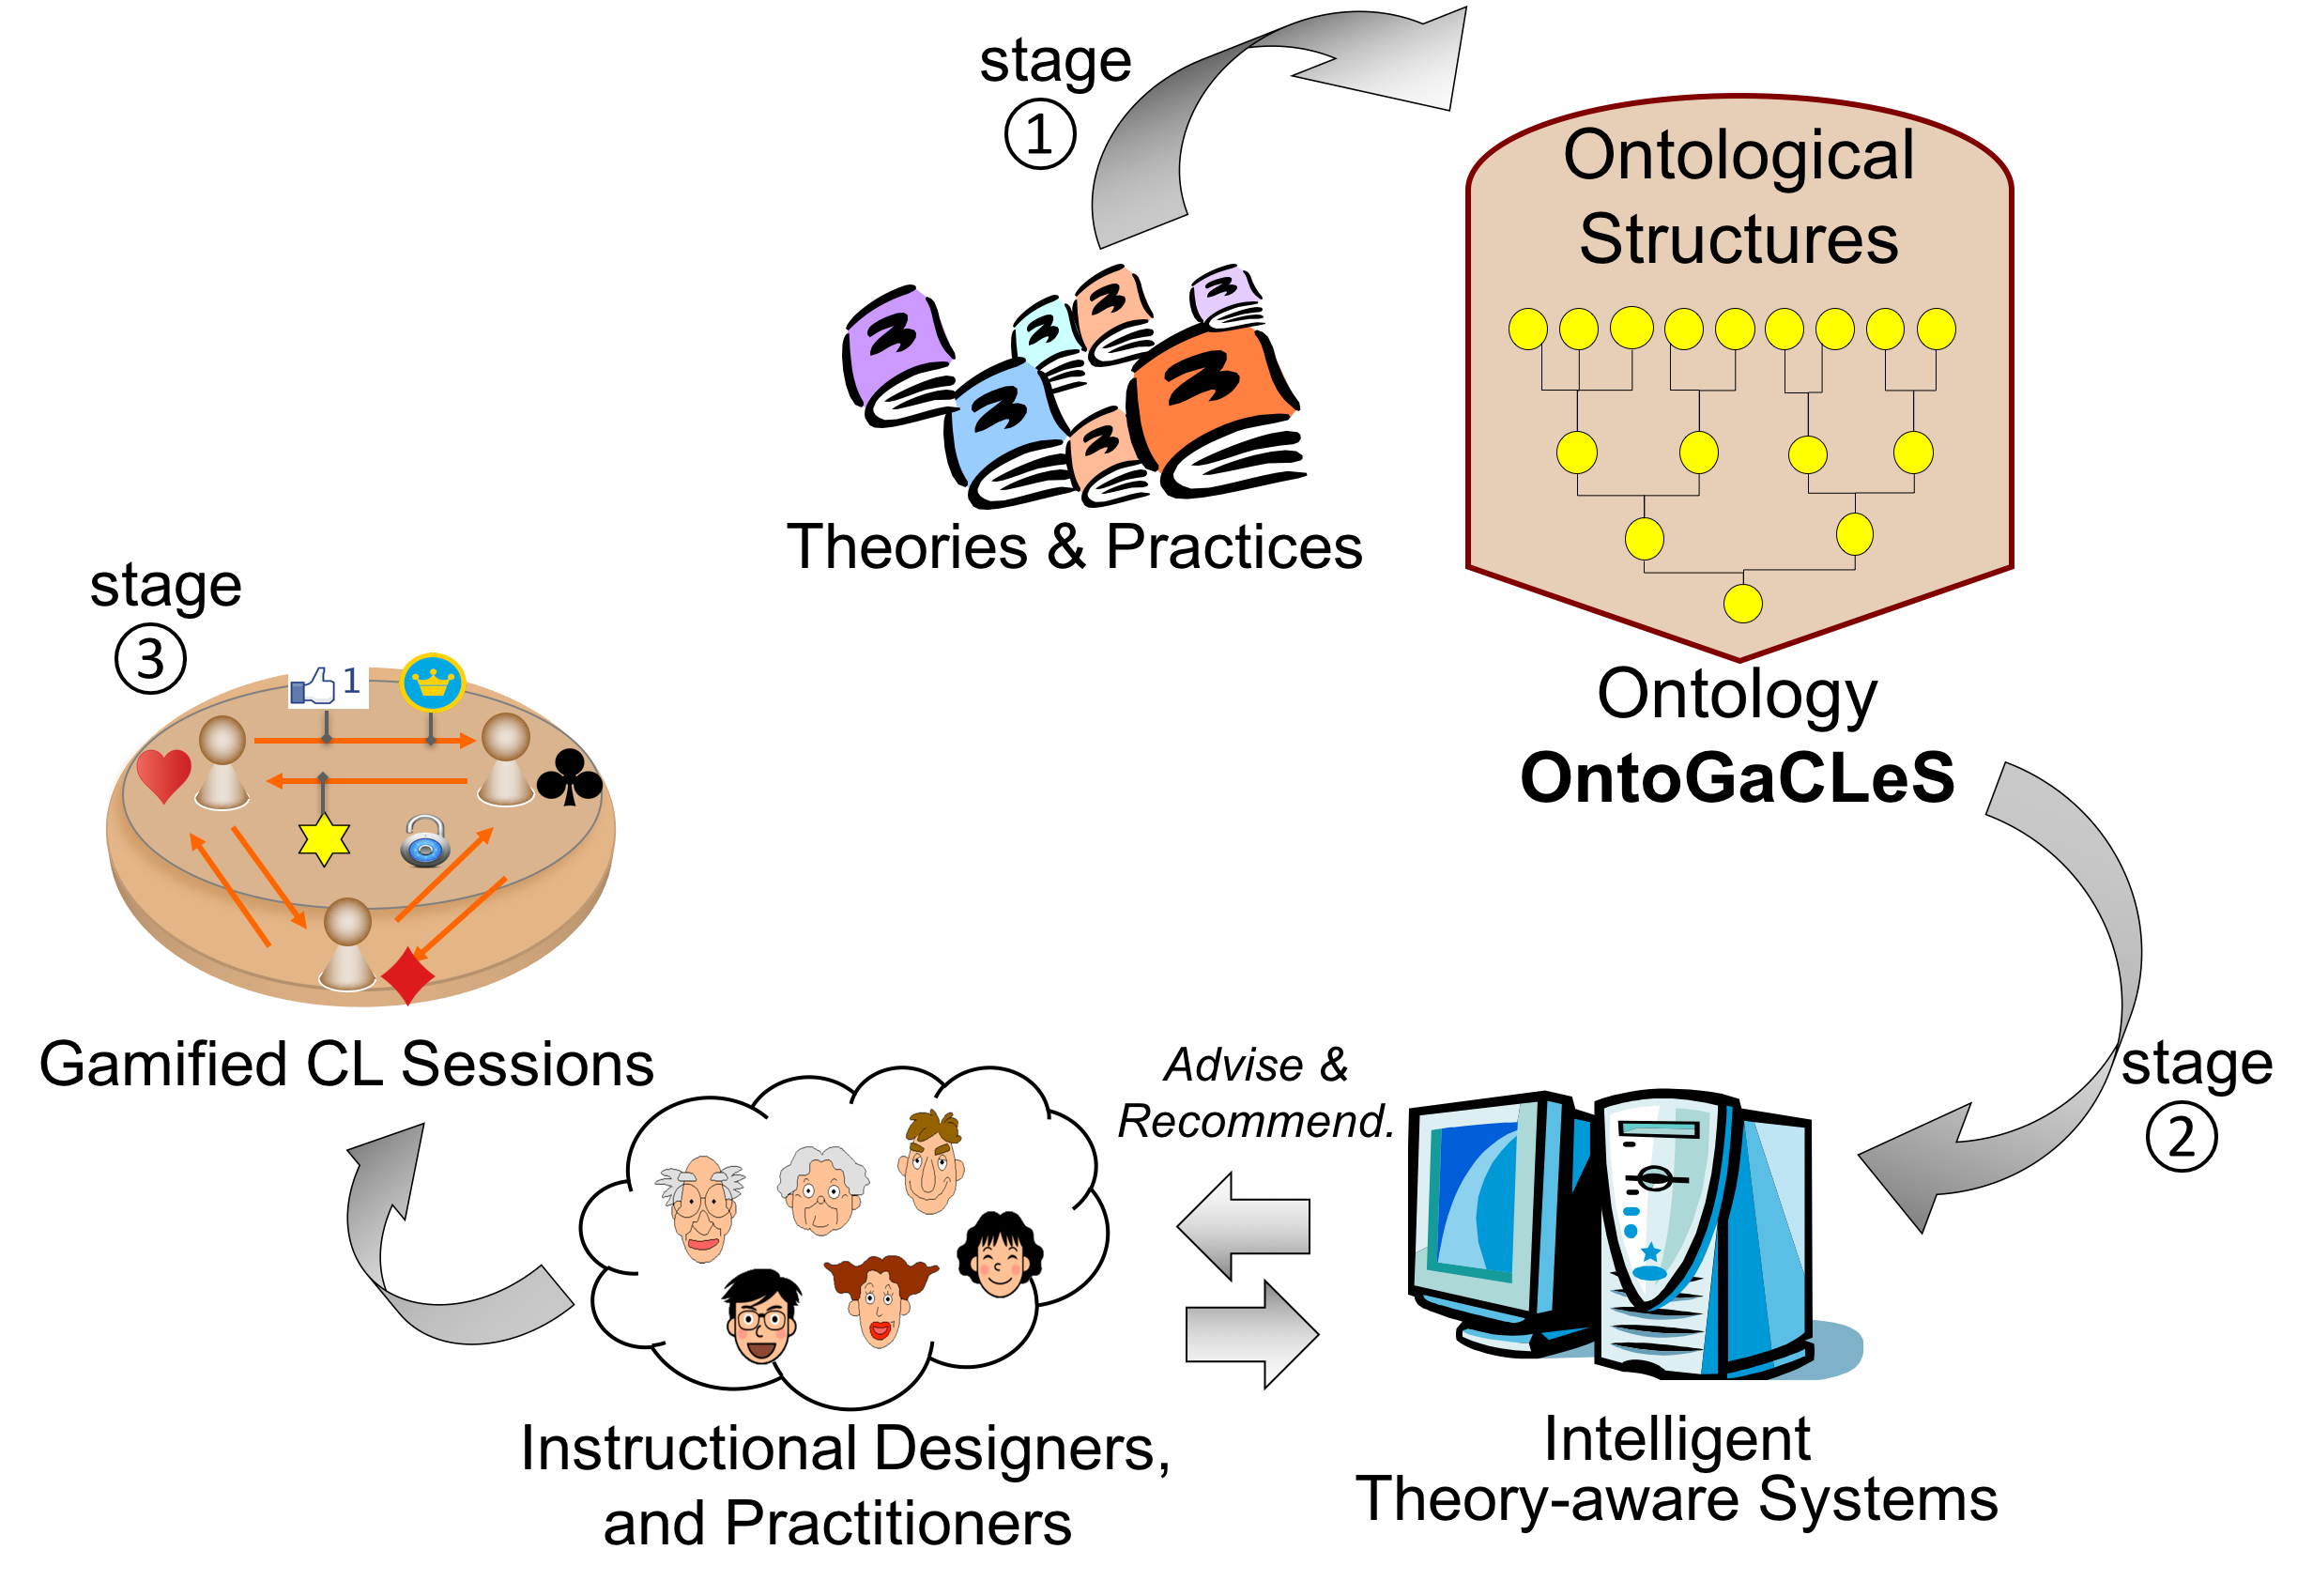
\includegraphics[width=0.95\textwidth]{images/chap-introduction/ontological-engineering-approach-to-gamify-cl-scenarios.png}
 \fautor
\end{figure}

\begin{enumerate}
\item
The first stage is: the formalization of the necessary knowledge about how to gamify CL scenarios for dealing with motivational problems in the scripted collaboration into an ontology named \textbf{OntoGaCLeS} – \emph{\textbf{Onto}logy to \textbf{Ga}mify \textbf{C}ollaborative \textbf{Le}arning \textbf{S}cenarios}. This ontology has been developed using ontology engineering in which, by extracting concepts from the theories and practices related to gamification, the thesis author defines a set of ontological structures to enable the systematic formalization and representation of knowledge to gamify CL scenarios and its theoretical foundation.

\item
The second stage is: the development of computational mechanisms and procedures whereby intelligent tools will provide support in the gamification of CL scenarios to deal with motivational problems in the scripting collaboration.
Such support is given by the knowledge formalized in the ontology OntoGaCLeS during the first stage, so that the purpose of the computational mechanisms and procedures in intelligent tools is to use the ontological structures from this ontology to facilitate the tasks of instructional designer and practitioners, especially novice users, in the gamification of CL scenarios. 
These ontological structures contain the theoretical justification for the personalization of gamification, and they are used to obtain tailored gamified CL sessions adapted for each situation.
Such sessions are known as ontology-based CL sessions, and they are CL scenarios that have been gamified and instantiated at the most concrete level of CL scenarios in which the participants and the content-domain to be learned are well defined to be directly run in a learning environment.

\item
The third stage is: the execution of empirical studies to understand the impact of gamification in CL scenarios, and then, to validate the ontological engineering approach to gamify CL scenarios as a method to deal with motivational problems in the scripted collaboration.
This validation is carried out in ontology-based gamified CL sessions obtained by the approach, and it consists in measuring the effectiveness and efficiency of these sessions for dealing with motivational problems.
\end{enumerate}

Regarding to the formalization of knowledge about how to gamify CL scenarios for dealing with motivational problems in the scripted collaboration (Stage 1), the research questions answered by this dissertation are:

\begin{description}
\item[RQ1:]
\emph{Which concepts from the theories and practices related to gamification should be taking into account to deal with motivational problems in the scripted collaboration?}, and
\emph{How should these concepts be applied in the gamification of CL scenarios?}

\item[RQ2:]
How can the concepts from the theories and practices related to gamification, and identified as relevant to deal with motivational problems caused by the scripted collaboration, be represented as ontological structures?

\end{description}

Regarding to the development of computer-based mechanisms and procedures whereby intelligent theory-aware systems will provide support in the gamified CL scenarios using the knowledge described in the ontology OntoGaCLeS (Stage 2), the research questions answered by this dissertation are:

\begin{description}
\item[RQ3:]
What computer-based mechanisms and procedure are necessary in intelligent-theory aware systems to give a helpful support in the gamification of CL scenarios? and How can the knowledge encoded in the ontology OntoGaCLeS be used by these mechanisms and procedures for dealing with motivational problems caused by the scripted collaboration?
\end{description}

Regarding to the validation of the ontological engineering approach to gamify CL scenarios as a method to deal with the motivational problems caused by the scripted collaboration (Stage 3), the research questions answered by this dissertation are:

\begin{description}
\item[RQ4:]
What are the effects of ontology-based gamified CL sessions on the students’ motivation and learning outcomes? and What are the effectiveness and efficiency of these sessions to deal with motivational problems caused by the scripted collaboration?
\end{description}

The research objectives pursued to answer the research questions \emph{RQ1} and \emph{RQ2} are:

\begin{description}
\item[RO1:]
To review the scientific literature in order to identify the most relevant concepts from the theories and practices related to gamification that should be taking into account to deal with motivational problems caused by the scripted collaboration, and how these concepts be applied in the gamification of CL scenarios; and

\item[RO2:]
To define the necessary ontological structures to represent the concepts identified as relevant in the scientific literature of gamification to deal with motivational problems caused by the scripted collaboration.
\end{description}


In order to answer the research question \emph{RQ3}, the research objectives is:

\begin{description}
\item[RO3:]
To identify and define the computer-based mechanisms and procedures that must be implemented by intelligent-theory aware systems to give a helpful support in the gamification of CL scenarios, and how these mechanisms and procedure use the knowledge encoded in the ontology OntoGaCLeS for dealing with the motivational problems caused by the scripted collaboration.
\end{description}

The research objective pursued to answer the research question \emph{RQ4} is:

\begin{description}
\item[RO4:]
to analyze the effects of ontology-based gamified CL sessions on the students’ motivation and learning outcomes for the purpose of validating the ontology engineering approach to gamify CL scenarios in reference to the effectiveness and efficiency to deal with the motivational problems caused by the scripted collaboration.
\end{description}

It is out of scope in this dissertation to deal with the following objectives:

\begin{itemize}
\item
To compare, validate or judge the practices and theories related to gamification.

\item
To create, modify or extend the concepts described in the practices and theories related to gamification.

\item
To create a generic and complete representation of all concepts described in the practices and theories related to gamification. The author of this thesis only concentrates on the formalization of the minimal necessary concepts from these practices and theories to deal with the motivational problems caused by the scripted collaboration.

\item
To validate the concepts and ontological structures formalized in the ontology OntoGaCLeS using semantic reasoner engines or formal methods based on logic and/or mathematics.
\end{itemize}

\section{Research Methodology}
\label{sec:research-methodology}

As this PhD thesis dissertation is framed in the multidisciplinary field of CSCL with research questions and research objectives oriented to be answered and achieved by theoretical and empirical studies, a mixed research method needs to be employed to conduct this research. Following the research methodology framework proposed by \citeonline{Glass1995,GlassVesseyRamesh2002}, the mixed research method employed in this PhD thesis research consists in four iterative phases: informational, propositional, analytical and evaluation.

\begin{description}
\item[Informational phase:]
In this phase, the research problems and potential solutions were identified based on information gathered from the scientific literature and discussions with experts in fields of CSCL, gamification and ontology engineering. The results of this phase were an outline of the knowledge involved in this dissertation, the research questions, and the research objectives. The tasks carried out in this phase correspond to tasks extracted from the scientific (observing the world) and engineering (observing existing solutions) research methods. These tasks were:

\begin{itemize}
\item
The search, review and analysis of scientific literature regarding to: CSCL, gamification and ontology engineering. This literature review was performed with emphasis in scripted collaboration, gamification of learning and instruction, and ontology-engineering applied to Artificial Intelligence in Education (AIED).

\item
The participation as member of the research group in Applied Computing in Education Laboratory (CAEd-Lab, \emph{Laboratorio de Computação Applicada a Educação e Tecnologias Sociales Avançadas}) at the University of São Paulo. Particularly, the expertise field in CSCL and Ontologies of this research group has been very important and valuable to conduct the research and the literature reviews.

\item
The participation in several conferences and workshops related to the context and problem domain in which this dissertation is framed. These conferences and workshop, in chronological order, were: the III Escola de Ontologias UFAL-USP, 2014 (Workshop); the 20\textsuperscript{th} International Conference on Collaboration and Technology, CRIWG, 2014 (Conference), the Summer School on Computers in Education, 2015 (Workshop); the XXVI Brazilian Symposium on Computers in Education, 2015 (Conference); the 6\textsuperscript{th} Latin American School for Education, Cognitive and Neural Sciences, 2016 (Workshop); and the Higher Education for All: International Workshop on Social, Semantic, Adaptive and Gamification techniques and technologies for Distance Learning, 2017 (Workshop).

\item
The participation as visiting research at the Research Center for Service Science at the School of Knowledge Science in the Japan Advanced Institute of Science and Technology (JAIST) has also been significant for the informational phase. This research center is dedicated to study, design and implementation knowledge co-creation process in complex service systems.  This research center focuses in the use of ontologies and ontology-engineering as the technology to develop and solve a broad variety of domains/tasks, and their research members have a long history working in the research field of Artificial Intelligence in Education. Particularly, the expertise of the Prof. Mitsuro Ikeda and Prof. Riichiro Mizoguchi were valuable and important for this phase due to their involvement in various research projects related to the modeling of knowledge for the students’ learning growth, CL process, and instructional design.
\end{itemize}

\item[Propositional phase:]
In this phase, solutions were proposed and formulated using the information gathered in the previous phase. As results of the propositional phase, constructors of necessary concepts to gamify CL scenarios were identified and proposed as ontological structures in the ontology OntoGaCLeS. Prototypes of computer-based mechanisms and procedures were also developed for gathering practitioner and user opinions as early feedback of these systems. The tasks carried out in this phase correspond to task extracted from the scientific (proposing theories or models) and engineering (proposing and developing solutions) research methods. These tasks were:

\begin{itemize}
\item
The proposal of ontological structures in the ontology OntoGaCLeS to represent gamified CL scenarios and ontological models to personalize the gamification of CL scenarios based on player type models and need-based theories of motivation.

\item
The proposal of ontological structures in the ontology OntoGaCLeS to represent the application of persuasive game design models in gamified CL scenarios and ontological models to apply persuasive game strategies as a method for dealing with the motivational problems caused by the scripted collaboration.

\item
The proposal of a computer-based model to unify the modeling of the learners' growth process and the flow theory based on the principle of good balance between the perceived challenges and skills.


\item
The definition of a conceptual flow to gamify CL scenarios as a computer-based procedure to use the knowledge described in the ontology OntoGaCLeS, and the definition of a reference architecture based on this flow to build computer-based mechanisms that provide support in intelligent-theory aware systems for dealing with the motivational problems caused by the scripted collaboration.
\end{itemize}

\item[Analytical phase:]
This phase consists into analyze and explore the solutions formulated in the propositional phase with the purpose to identify whether the proposed solutions are understandable, how them can be deployed into practice, what are the potential problems in understanding and using them, and wether there are any omissions or gaps in these solutions. The tasks carried out in this phase correspond to task extracted from the empirical (applying to case studies) and analytical (developing new solutions derived from the results obtained in the case studies) research methods. These tasks were:

\begin{itemize}
\item
The formalization of an ontological model to personalize the gamification of CL scenarios based on the Dodecad player type model proposed by \citeonline{Marczewski2015b}, and the formalization of an ontological model to personalize the gamification of Cognitive Apprentice CL scenarios based on the Yee's player type model. These two formalizations were developed as case studies to validate in the evaluation phase the ontological structures proposed to systematically formalize ontological models to personalize the gamification of CL scenarios.

\item
The formalization of an ontological model to apply gamification as a persuasive technology in gamified Cognitive Apprenticeship scenarios employing the persuasive game design strategies defined in the Model-driven persuasive game proposed by \citeonline{Orji2014}.

\item
The implementation of a computer-based mechanism (as a proof of concept) in which the knowledge encoding in the ontology OntoGaCLeS is used for setting up the proper player roles and game elements for CL sessions.

\item
The development of an algorithm (as a proof of concept) to apply the principle of good balance between the perceived challenges and skills from the flow theory in the gamification of CL scenarios.

\item
The development of a computer-based mechanisms (as a proof of concept) to apply gamification as persuasive technology in the gamification of CL scenarios. 
\end{itemize}


\item[Evaluation phase:]
The focus of this phase is to conduct empirical tests and evaluations for the solutions formulated in the propositional phase and for the findings found in the analytical phase. In this phase, the empirical data gathered through the tests and evaluations aim to assess the contributions from different perspectives. The task carried out in this phase correspond to task from the empirical (validating the solutions) and analytical (analyzing the results obtained from empirical observations) research methods. These tasks were:

\begin{itemize}
\item
The analytical evaluation of the ontological structures proposed to represent gamified CL scenarios and the ontological models to personalize the gamification of CL scenarios. This evaluation was carried out by publishing these ontological structures and the ontological models obtained from them in the analytical phase (the ontological model to personalize gamification in CL scenarios based on the Dodecad player type model, and the ontological model to personalize gamification in Cognitive Apprentice CL scenarios based on the Yee's player type model) as scientific articles in conferences and journals related to the fields of CSCL, and Artificial Intelligent in Education. These articles, in chronological order, were: \aspas{\emph{Towards an Ontology for Gamifying Collaborative Learning Scenarios}} published in the 12\textsuperscript{th} International Conference on Intelligent Tutoring Systems, ITS, 2014; \aspas{\emph{An Ontology Engineering Approach to Gamify Collaborative Learning Scenarios}} published in the 20\textsuperscript{th} International Conference on Collaboration and Technology, CRIWG, 2014; and \aspas{\emph{Personalization of Gamification in Collaborative Learning Contexts using Ontologies}} published in the journal of IEEE Latin America Transactions, 2015. During the conferences important feedbacks to improve the ontological structures were obtained from informal discussions with the participants of the conferences who shared their expertise in the domain of CSCL and Artificial Intelligent in Education.

\item
The analytical evaluation of the ontological structures proposed to represent the application of persuasive game design models in gamified CL scenarios and the ontological models to apply persuasive game strategies as a method for dealing with motivational problems caused by the scripted collaboration. This evaluation was carried out by publishing these ontological structures and the ontological models obtained from them in the analytical phase (the ontological model to apply gamification as a persuasive technology in gamified Cognitive Apprenticeship scenarios employing the persuasive game design strategies defined in the Model-driven persuasive game) as scientific articles scientific articles in conferences and journals related to the fields of CSCL, and Artificial Intelligent in Education. These articles, in chronological order, were: \aspas{\emph{Steps Towards the Gamification of Collaborative Learning Scenarios Supported by Ontologies}} published in the 17\textsuperscript{th} International Conference on Artificial Intelligence in Education, AIED, 2015; \aspas{\emph{An Ontological Model to Apply Gamification as Persuasive Technology in Collaborative Learning Scenarios}} published in the 26\textsuperscript{th} Brazilian Symposium of Informatics in Education, SBIE, 2015; \aspas{\emph{Gamification of Collaborative Learning Scenarios: Structuring Persuasive Strategies Using Game Elements and Ontologies}} published in the 1\textsuperscript{st} International Workshop of Social Computing in Digital Education, SOCIALEDU, 2015; and \aspas{\emph{An Ontology Framework to Apply Gamification in CSCL Scenarios as Persuasive Technology}} published in the Brazilian Journal of Computers in Education, 2016. During the conferences important feedbacks to improve the ontological structures were obtained from informal discussions with the participants of the conferences who shared their expertise in the domain of CSCL and Artificial Intelligent in Education.

\item
The conduction of a pilot empirical study in which, prior to carry out the full-scale empirical studies, the activities, methods, instruments and activities that have been used in the full-scale studies were evaluated to adjust and improve the full-scale study design. This empirical study has been conducted to assess the effectiveness of \emph{the ontological engineering approach to gamify CL scenarios} for dealing with the motivational problems caused by the scripted collaboration. Such effectiveness is measured by comparing the effect of the ontology-based CL sessions obtained by the approach against the effect of non-gamified CL sessions on the participants' intrinsic motivation and learning outcomes, and the percentage of participation by groups. This empirical study was conducted with undergraduate computer science students at the university of São Paulo during the second semester of 2016 in the course of Laboratory of Introduction to Computer Science, and for a CL activity related to the topic of loop structures. In such CL activity, the ontology-based gamified sessions and non-gamified CL sessions have been instantiated using a CSCL script inspired by the cognitive apprenticeship theory as the method to orchestrate and structure the collaboration among the students.

\item
The conduction of a full-scale empirical to evaluate the effectiveness of \emph{the ontological engineering approach to gamify CL scenarios}. This effectiveness has been measured by comparing the effects of ontology-based gamified CL sessions against the effects of non-gamified CL sessions on the participants' intrinsic motivation and learning outcomes. This study was carried out in the course of introduction to computer science with undergraduate computer engineering students at the university of São Paulo during the first semester of 2017. The CL activity in which these CL sessions have been instantiated was related to the topic of condition structures using a CSCL script based on the cognitive apprentice theory to orchestrate and structure the collaboration among the participants.

\item
The conduction of a full-scale empirical study to also evaluate the effectiveness of \emph{the ontological engineering approach to gamify CL scenarios}.
However, in this empirical study, the effects of ontology-based gamified CL sessions against the effect of non-gamified CL sessions were compared on the participants' level of motivation instead to compare these effects on the participants' intrinsic motivation. This empirical study was carried out during the first semester of 2017 in the course of Introduction to Computer Science at the university of São Paulo with undergraduate computer engineering students. In this context, a CSCL script inspired by the cognitive apprentice theory was used to structure and orchestrate the collaboration among the students a CL activity related to the the topic of loop structures.

\item
The conduction of a full-scale empirical study to evaluate the efficiency of \emph{the ontological engineering approach to gamify CL scenarios} for dealing with motivational problems in the scripted collaboration.
Such efficiency was measured by comparing the participants' motivation and learning outcomes in ontology-based CL sessions against the participants' motivation and learning outcomes in CL sessions that have been gamified without using the support given by the ontology OntoGaCLeS.
\end{itemize}
\end{description}

\section{Thesis Statement and Claimed Contributions}
\label{sec:thesis-statement-and-claimed-contributions}

The thesis statement of this PhD thesis dissertation is that:

\aspas{\emph{For CL activities where the CSCL scripts are used as a method to orchestrate and structure the collaboration among the participants, the ontological engineering approach to gamify CL scenarios, understood from the viewpoint of an instructional designer as the gamification of CL scenarios in which the ontology OntoGaCLeS is used as support to personalize the gamification, constitutes an effective and efficient solution to deal with motivational problems}.}

Related to this thesis statement, the claimed contributions that are discussed throughout this PhD thesis dissertation are:

\begin{enumerate}
\item 
The identification of relevant concepts from the theories and practices related to gamification that should be taking into account to deal with motivational problems in the scripted collaboration (RO1).

\item
Ontological structures to represent: the concepts identified as relevant in theories and practices related to gamification for dealing with motivational problems in the scripted collaboration (RO2).

\begin{enumerate}
\item
Ontological structures to represent: gamified CL scenarios, and ontological models to personalize the gamification of CL scenarios based on player types models and need-based theories of motivation.

\item
Ontological structures to represent: persuasive game design in CL scenarios, and ontological models to apply persuasive game design strategies as a method for dealing with the motivational problems in the scripted collaboration.
\end{enumerate}

\item 
A computer-based model to support the representation of the learners' growth process and the principle of good balance between challenges and abilities defined in the flow theory.

\item
A conceptual flow to gamify CL scenarios using the knowledge described in the ontology OntoGaCLeS, and a reference architecture based on this flow to build intelligent tools that provide theoretical support for dealing with motivational problems in the scripted collaboration (RO3).

\item
Empirical evaluations of \emph{the ontological engineering approach to gamify CL scenarios} in which, to validate the effectiveness and efficiency of this approach to deal with motivational problems, the participants' motivation and the learning outcomes in ontology-based gamified CL sessions are compared against the participants' motivation and the learning outcomes in non-gamified CL sessions and in CL sessions that have been gamified without the support given by the ontology (RO4).
\end{enumerate}

\section{Structure of the Dissertation}
\label{sec:structure-of-dissertation}

This PhD thesis dissertation is structured in eight chapters that are described as follow:

\begin{description}

\item[Chapter 1:]
\emph{Introduction}

\item[Chapter 2:]
\emph{General Background and Fundamental Concepts} contains the background related to the research problem addressed in this dissertation.
An overview related to the fields of CSCL and scripted collaboration, gamification and ontology engineering are presented in the chapter.
The motivational problems in the scripted collaboration and the current approaches to deal with these problem are detailed in the chapter.
The concepts that were identified as relevant in the theories and practices to deal with the motivational problems through gamification of CL scenarios are presented in the chapter.

\item[Chapter 3:]
\emph{Ontological Structure to Personalize the Gamification in CL Scenarios} describes the ontological structures that have been formalized in the ontology OntoGaCLeS to represent gamified CL scenarios.
These ontological structures support the personalization of gamification in CL scenarios based on player types models and need-based theories of motivation.
Therefore, the chapter also shows the procedure followed by the thesis author to build an ontological model ontological model to personalize the gamification of CL scenarios based on the Dodecad player type model and Self-determination theory.

\item[Chapter 4:]
\emph{Ontological Structures of Persuasive Game Design in CL Scenarios} describes the ontological structures proposed to apply persuasive game design models in CL scenarios.
The chapter also describes the procedure employed by the thesis author to formalize an ontological model to apply gamification as persuasive technology in Cognitive Apprenticeship scenarios.

\item[Chapter 5:]
\emph{A Unify Modeling of Learners' Growth Process and Flow Theory} presents the computer-based model proposed to unify the modeling of the learners' growth process and the principle of good balance between the perceived challenges and skills described in the flow theory.
This model has been used in the gamification of CL scenarios to define the reward levels that are given in the CL process as a attempt to maintain the flow states of participants.

\item[Chapter 6:]
\emph{Computer-based Mechanisms and Procedures to Gamify CL Scenarios} describes a flow proposed to gamify CL sessions based on the knowledge described in the ontology OntoGaCLeS.
Based on this flow, a reference architecture by which intelligent tools to provide support in the gamification of CL scenarios for dealing with motivational problems is presented in the chapter.
The chapter also describes the computational mechanisms and procedures that has been developed based on the reference architecture to conduct the evaluation of the ontological engineering approach to gamify CL scenarios.

\item[Chapter 7:]
\emph{Evaluation of the Ontological Engineering Approach to Gamify CL Scenarios} presents the empirical studies that have been carried out in real situations to validate the effectiveness and efficiency of this approach to deal with motivational problems.

\item[Chapter 8:]
\emph{Conclusions and Future Work} summarizes the contributions of this PhD thesis dissertation, and the chapter also discusses possible future research directions.

\end{description}


\chapter{General Background and Fundamental Concepts}
\label{chapter:general-background}
%This Chapter presents the general background and fundamental concepts related to the domain problem that is addressed in this thesis. At the first section (\autoref{sec:cscl-and-scripted-collaboration}), an overview of CSCL field and scripted collaboration is presented to provide a most comprehensive and clear understanding about the research context. This section also describes in detail the motivation problem caused by the scripted collaboration when CL activities are orchestrated and structured by CSCL scripts, as well as, the related works and current computer-based solutions to deal with this problem. The \autoref{sec:gamification} elaborates an overview of gamification, and the best practices and theories related to this technology. Furthermore, the related works that use gamification in the context of CSCL and other contexts to deal with the motivation problem are presented in this section. Finally, the \autoref{sec:ontologies-and-ontology-engineering} presents the fundamentals of ontologies and ontology engineering. This sections also discusses how ontologies is currently used to support the systematic formalization of theory-based knowledge, and how this formalization, in the field of artificial intelligence in education, is used to overcome some problems that are similar to those that must be solved to provide a computational support in the gamification of CL scenarios with theoretical justifications based on the best practices and theories related to gamification. 

\section{CSCL and Scripted Collaboration}
\label{sec:cscl-and-scripted-collaboration}

Although CL has a long history in education, it is not until the early 1990s that the research field dedicated to study how to provide support for the CL through the use of Internet and computational technology had gained attention and strength \cite{StahlKoschmannSuthers2006}. Such research field known as Computer-Supported Collaborative Learning (CSCL) is a multidisciplinary field that combines studies from the cognitive psychology education and from the computer science to effectively enhance the CL process through the use of computational technology \cite{HoppeOgataSoller2007}.

The general aim of CSCL field is to develop technologies to support or create situations in which two or more students learn together through the interaction among them \cite{Dillenbourg1999}. In these situations, the learning outcomes is consequence of students' interactions and how these interactions affect the individual learning for each one of the students. In consequence, to enable a well-though-out design of CL, the CSCL scripts have been proposed by the CSCL community as the technology to facilitate the social and cognitive processes of learning by describing the way in which the learners will interact with each other in a CL scenario \cite{HarrerKobbeMalzahn2007}.

\subsection{CSCL Scripts}
\label{sec:cscl-scripts}

CSCL scripts are the technology that describes how to structure and orchestrate the CL process to attain a set of pedagogical objectives defined by an instructional design \cite{DillenbourgJermann2007}. Such description is provided in the CSCL scripts through prescribed instructions that indicates how to facilitate the social and cognitive processes in group activities \cite{Dillenbourg2002}. These prescribed instructions are defined by instructors, like teachers or instructional designers, as a way to attain a set of learning goals, and they indicate the way in which students should collaborate, they constrain the interactions among the participants, they specify the roles for the participants, they indicate the distribution of task, tools, and resources used in the CL process.

In order to narrow the number of elements used to describe the CSCL scripts, and provide a common and sharable description of CSCL scripts, \citeonline{KobbeWeinbergerDillenbourgHarrerHamalainenHakkinenFischer2007} propose a framework that is currently wide accepted by the community as the common specification to describe the CSCL scripts using natural language. This framework formalizes the CSCL scripts as a set of components and mechanisms illustrate in \autoref{fig:components-and-mechanisms-of-cscl-scripts}.


\begin{figure}[htb]
 \caption{Components and mechanisms of CSCL scripts}
 \label{fig:components-and-mechanisms-of-cscl-scripts}
 \centering
 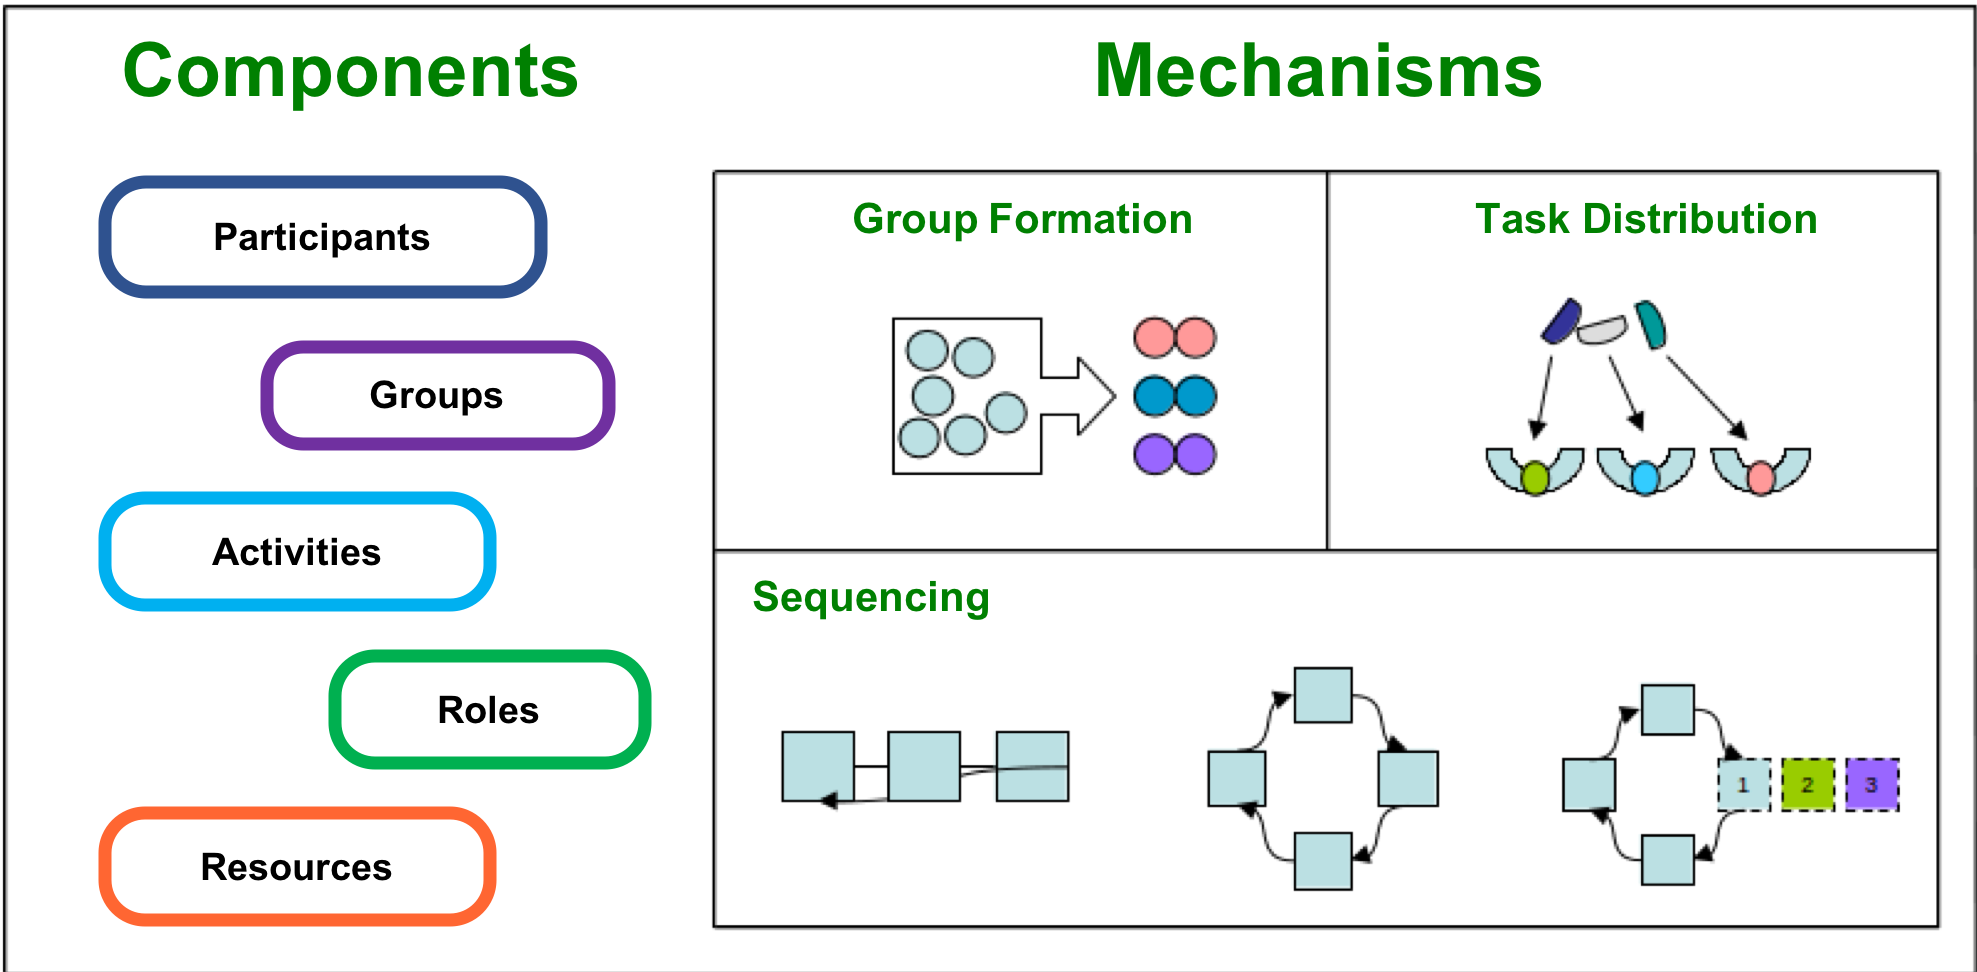
\includegraphics[width=0.95\textwidth]{images/components-and-mechanisms-of-cscl-scripts}
 \fadaptada{Fischer2007}
\end{figure}

The structural \emph{components} of CSCL scripts are the participants, groups, activities, roles and resources. The component of \emph{participants} is used to describe the participants, such as learners, monitors, and teachers. Although this description can be abstract or concrete and simple or complex, it is often presented in a simple manner with rules that indicate conditions to participate in the CL process. The component of \emph{activities} describes what will be performed by the participants in the CL process to attain the learning goals defined by the instructional designers. The component of \emph{roles} describes the privileges, obligations and expectations of participants in the CL process. The component of \emph{groups} of participants defines through hierarchical structures how the students are grouped according to the participants' characteristics. The component of \emph{resources} describes the learning objects (e.g. content, material, and tools) that can be used by the participants during the CL process.

The \emph{mechanisms} of CSCL scripts are the group formation, component distribution and sequencing. The mechanism of \emph{group formation} consists in the specifications of how the participants will be distributed over the groups. The mechanism of \emph{task distribution} provides the specification about how the components of scripts are distributed over groups using the mapping of groups, activities, roles, and resources. The mechanism of \emph{sequencing} consists in the definition of how the components and groups defined in scripts are distributed over time. In general, this sequencing describes the execution order of activities in the CL process.

\autoref{qua:social-script-framework-kobbe} shows the description of social script \cite{WeinbergerErtlFischerMandl2005} using the framework proposed by \citeonline{KobbeWeinbergerDillenbourgHarrerHamalainenHakkinenFischer2007}. In this example, the CL scenarios orchestrated by the social script foster the acquisition of knowledge through a set of case studies (\emph{resources}) that are analyzed and reviewed by the students groups. The number of students in each group is equal to the number of case studies, and the ideal number is three. In the first step of sequencing, each learner playing the \emph{analysis} role writes down an analysis of case study, and then, he critiques the analyses made by other learners playing the \emph{critics} role. In the second step of sequencing, each learner revises his/her own analysis, taking into consideration the critiques received by the other learners in the case group.

\begin{quadro}[htb]
\caption{Social script describes using the framework proposed by  \citeonline{ KobbeWeinbergerDillenbourgHarrerHamalainenHakkinenFischer2007}}
\label{qua:social-script-framework-kobbe}
\centering
\footnotesize
\begin{tabular}{l p{12cm}}
\toprule
\multicolumn{2}{l}{\textbf{Structural components:}} \\ \midrule
\textbf{Participants:} &
A number of participants that must be divisible by the number of case studies.  \\
\textbf{Groups:} &
Case groups \\
\textbf{Activities:} &
(a) Applying theoretical concepts to the case study and constructing arguments \\
 &
(b) Critiquing initially scaffolder with prompts for eliciting clarification, identifying conflicting views and constructing counter-arguments \\
\textbf{Roles:} &
\emph{Analyst} and \emph{Critic} \\
\textbf{Resources:} &
Case studies (minimal number is three case studies) \\
\toprule
\multicolumn{2}{l}{\textbf{Mechanisms}:} \\ \midrule
\textbf{Group formation:} &
All participants are grouped by the number of case studies. Each participant becomes member of all case groups although with different roles in each. Each participant is the responsible analyst for one case study and critic for all other cases \\
\textbf{Task distribution:} &
Each case group receives one case study, and the roles are distributed in a way that each participant assumes the role of analyst in one case group and the role of critic in all other case groups \\
\textbf{Sequencing:}
& - the analyst writes an analysis of case study. (a) \\
& - wait for all case group analysts to be done, and writes a critique for the analysis of case study. (b) \\
& - wait for all case group critics to be done, and the analyst considers each critique and writes a reply to each. (a) \\
& - wait for all case group analysts to be done each critic in turn reads the reply and writes a second critique. (b) \\
& - wait for all case group critics to be done... the analyst considers all critiques and revises the analysis of case study (a) \\
\bottomrule
\end{tabular}
%\fadapted{KobbeWeinbergerDillenbourgHarrerHamalainenHakkinenFischer2007}
\end{quadro}


Having the description of CSCL scripts only in natural language does not allow the computers programs to interpret them, and to run a CL scenario following the instructions indicated by the scripts without human intervention. Therefore, to represent the CSCL scripts in a computer readable manner, the IMS-Learning Design\footnote{\url{http://www.imsglobal.org/learningdesign/}} (IMS-LD) specification has been adopted by different tools, such as (web)COLLAGE \cite{Hernandez-LeoVillasclaras-FernandezAsensio-PerezDimitriadisJorrin-AbellanRuiz-RequiesRubia-Avi2006,Villasclaras-FernandezHernandez-LeoAsensio-PerezDimitriadis2013}, CIAN \cite{MolinaRedondoOrtega2012}, LeadFlow4LD \cite{Palomino-RamirezBote-LorenzoAsensio-PerezDimitriadis2008}, NUCLEO \cite{SanchoFuentes-FernandezFernandez-Manjon2008}, CoLearn \cite{StylianakisArapiMoumoutzisChristodoulakis2013}, CeLS \cite{RonenKohen-Vacs2009}, and LAMS \cite{Romero-MorenoOrtegaTroyano2007}, as the language to describe CSCL scripts.
 
Despite the benefits that brings  the use of the IMS-LD specification to represent CSCL scripts, several researchers had indicated that this language is insufficient to fully support the modeling of CSCL scripts \cite{AlharbiAthaudaChiong2014, CaeiroAnidoLlamas2003}. Of course, the purpose of IMS-LD specification is not to provide a full support for describing CSCL scripts in a computer-readable manner, the IMS-LD has been developed as a neutral, generic and flexible educational modeling language to describe a wide range of pedagogies approaches (the teaching strategies, pedagogical goals and their associated activities) \cite{Koper2005}. In this sense, to support the representation of CSCL scripts in a computer-readable manner, a wide variety of extensions on the IMS-LD elements has been proposed in by several researchers \cite{Bote-LorenzoVaquero-GonzalezVega-GorgojoDimitriadisAsensio-PerezGomez-SanchezHernandez-Leo2004, LeoPerezDimitriadis2004, MagnisalisDemetriadis2012, MiaoHoeksemaHoppeHarrer2005, Vega-GorgojoBote-LorenzoGomez-SanchezDimitriadisAsensio-Perez2005}.

Instead, to simply provide a computer-readable representation of CSCL scripts, the work of \citeonline{Isotani2009} proposes the formalization of these scripts in a computer-understandable manner through the use of ontologies. This solution consists in a set of ontological structures that makes the description of CSCL scripts more semantically-rich, allowing the explicit specification of learning goals, purposes, and other relevant information that cannot be represented using the IMS-LD specification, i.e., learning strategies, group goals, interaction patters from learning theories. Providing this formalization in the CL ontology, \citeonline{IsotaniMizoguchiIsotaniCapeliIsotanideAlbuquerqueBittencourtJaques2013} demonstrates that intelligent-theory aware systems can interpret these scripts and provide advice and recommendation to support for the modeling of learners' development \cite{InabaIkedaMizoguchi2003}, the formation of effective groups \cite{IsotaniMizoguchi2008a}, and the instructional design of CL activities \cite{IsotaniMizoguchiIsotaniCapeliIsotanideAlbuquerqueBittencourtJaques2013}.

\subsection{Levels of Abstraction and Granularity of CSCL Scripts}
\label{sec:level-of-abstraction-and-granularity-of-cscl-scripts}

CSCL scripts have different levels of abstraction and granularity in the description of CL scenarios \cite{Dillenbourg2002, DillenbourgJermann2007, Villasclaras-FernandezIsotaniHayashiMizoguchi2009}. This classification of scripts in two dimension, abstraction and granularity, gives them an enormous flexibility to be reused in the instructional design process of CL scenarios, and it also allows the use of multiple scripts to describe different aspects of CL scenario in separated scripts. Whereas the levels of abstraction classify a script according to the completeness of elements described by them (from the most abstract to the most concrete), the levels of granularity classify the scripts according to the aggregation level of elements described by them (from the most coarser grained to the finest grained).

According to \citeonline{DillenbourgJermann2007}, a CSCL script can be classified in one of the four levels of abstraction defined as follows as:

\begin{description}
\item[\emph{Script Schemata}:] are scripts use to describe the core instructional design principles whereby is expected to trigger interactions among participants in the CL process. In this sense, these scripts are defined in a content free didactic form, so that they can be used to describe patterns of CL. Examples of script schemata are the Jigsaw script \cite{Aronson1978, KordakiSiempos2010}, conflict script \cite{WeinbergerErtlFischerMandl2005}, and reciprocal script \cite{King2007}. The jigsaw script describes a CL scenario in which the principle of interaction consists in the grouping and re-grouping of participants with complementary information to share their knowledge. The conflict script describes a CL scenario to group learners with contradictory knowledges or opinions to instigate the discussion. The reciprocal script describes a CL scenario that assigns alternate roles to the students for facilitating questioning and tutoring activities.

\item[\emph{Script Classes}:] are specialization of scripts schemata for a specific learning context. This specialization is not absolute complete, so that script classes are independent in the content-domain and student data. The script classes cover a range of scripts that describe variations of a prototype with particular details related to a specific learning context of a script schemata to facilitate its adoption. These details are, for example, the number of participants, and the king of content (matter) that will be taught. In this sense, a script class is based in a script schemata to describe CL scenarios for a specific learning context. For instance, the Universanté Script \cite{DillenbourgJermann2007} is a script class based on Jigsaw schema that was designed to describe CL scenarios for learning contexts with different thematic groups and participants from different nations.

\item[\emph{Script Instances}:] are scripts in which the content-domain are specified for a particular situation. A script instance is more concrete than a script class, and it has been instantiated from a script schema or class to be reusable more or less by teachers who only need to define participants' data. These scripts are more concrete that script classes, but they are independent in the particularities of students and learning environment.

\item[\emph{Script Sessions}:] are scripts in which the content-domain and participants data are specified to be directly executed in a learning environment. In this sense, these scripts detail the information of participants and content-domain in the most concrete level defining, for example, the students' names and the deadlines of activities. A CL scenario that is described by a script session is known as CL session, and when it is represented in a script session using a computer-readable formalization, it can be directly executed in a learning environment to orchestrate and conduct the CL process.
\end{description}

Different benefits from the use of script schemata and classes as patterns are obtained in the instructional design process of CL scenarios \cite{AlharbiAthaudaChiong2014, ChallcoBittencourtIsotani2016, MiaoHoeksemaHoppeHarrer2005}. During the design/authoring phase, repositories of script schemata and classes facilitate the sharing and reuse of these scripts in distributed learning environments \cite{PrietoAsensio-PerezMunoz-CristobalDimitriadisJorrin-AbellanGomez-Sanchez2013, PrietoTchounikineAsensio-PerezSobreiraDimitriadis2014}. The structures of script schemata and classes are used as templates to create new script schemata and classes \cite{AndreasHarrerH.UlrchHoppe2007, RonenKohen-Vacs2009}. 

During the instantiation/production phase, script schemata and classes provide advice and recommendation that help the CL practitioners to instantiate these scripts and to obtain CL sessions \cite{MagnisalisDemetriadis2012a, PrietoAsensio-PerezDimitriadisGomez-SanchezMunoz-Cristobal2011,Alario-HoyosBote-LorenzoGomez-SanchezAsensio-PerezVega-GorgojoRuiz-Calleja2013}. Script schemata and classes facilitate the generation of computer-interpretable scripts, they provide information to support the search of applicable learning material and tools for the CL scenario \cite{Bote-LorenzoVaquero-GonzalezVega-GorgojoDimitriadisAsensio-PerezGomez-SanchezHernandez-Leo2004, IsotaniMizoguchi2008a, Vega-GorgojoBote-LorenzoGomez-SanchezDimitriadisAsensio-Perez2005}. The script schemata and classes are also uses to obtain recommendation about how to bind individuals in groups and roles according to the knowledge described in these scripts \cite{IsotaniMizoguchiIsotaniCapeliIsotanideAlbuquerqueBittencourtJaques2013,Villasclaras-FernandezHernandez-GonzaloLeoAsensio-PerezDimitriadisMartinez-Mones2009}.

Regarding to the level of granularity \cite{FischerKollarStegmannWeckerZottmann2013}, the CSCL scripts can be classified in macro-scripts and micro-scripts.

\begin{description}
\item[\emph{Macro-scripts}:] are scripts that basically describe the CL process in a courser-grained level without detailing the specific interactions among participants. A macro-script describes how to attain a set of pedagogical objective indicating the sequencing of individual and group activities that must be follow by participants. Thus, for example, in the Jigsaw macro-script, to promotes the individual accountability and positive interdependence, the sequencing of activities consists in three activities: an individual activity, expert group activity, and jigsaw group activity. In the individual activity, each student studies a particular part of a whole problem. In the expert group, the students of different groups that study the same part of the whole problem meet together for exchanging ideas. At last activity, students of each jigsaw group meet to contribute with their expertise to solve the whole problem.

\item[\emph{Micro-scripts}:] are scripts that describe the CL process in a fine-grained level \cite{WeinbergerFischerStegmann2005}, they indicate, for example, the dialogues that must happen among student to achieve the pedagogical objectives, and they are intended to describe the communication model between participants. Thus, for example, to facilitate the negotiation and elaboration of a domain concepts, Weinberger, Ertl, Fischer, and Mandl  \cite{WeinbergerErtlFischerMandl2005} describe a micro-scripts for online peer discussion using a sequence of sentence openers (e.g. my proposal for an adjustment of the analysis is….) that prompted learners to contribute with the discussion and critique one another's contributions.
\end{description}

As can be noticed above, the macro-scripts and micro-scripts have a hierarchical relationship to describe the CL process of CL activities. The micro-scripts describe the communication process in a CL activity \cite{WeinbergerFischerStegmann2005}, whereas the macro-scripts describe groups, roles, and flow of CL activities \cite{DillenbourgHong2008}. Despite this explicit hierarchical relationship, there are few models and tools in which all the elements of macro-scripts and micro-scripts are combined to support the design of CL scenarios \cite{AlharbiAthaudaChiong2014, ChallcoBittencourtIsotani2016}. \citeonline{Hernandez-LeoVillasclaras-FernandezAsensio-PerezDimitriadisRetalis2006} propose a hierarchical model in which schemata and classes of macro-scripts and micro-scripts are used as templates to generate scripts. In the work of \citeonline{ChallcoGerosaBittencourtIsotani2014}, the hierarchical relationships of macro-scripts and micro-scripts is represented as hierarchical task networks to support the automatic generation of unit of learning.

In the CL ontology \cite{IsotaniInabaIkedaMizoguchi2009}, and therefore in the ontology OntoGaCLeS, the hierarchical relationship of macro-scripts and micro-scripts is not explicitly described as a direct link between macro- and micro-scripts. The hierarchical relationship is implicitly described as part of the conceptualization of events and processes proposed by Galton and Mizoguchi \cite{GaltonMizoguchi2009}. Based on in this conceptualization in which the representation of an event can be constituted by many distinct sub-events to describe a process, the hierarchical relationship of macro- and micro-scripts can be inferred from these events that are explicitly described in the CL ontology and the ontology OntoGaCLeS.


\section{Gamification of Learning and Instruction}
\label{sec:gamification}

\section{Ontologies and Ontology Engineering}
\label{sec:ontologies-and-ontology-engineering}

This formalization is achieved through ontology engineering in which the similarities and differences of these concepts are identified to describe their application in the gamification of CL scenarios and the building of gamification model for CL scenarios.




\chapter[Ontological Structures to Personalize the Gamification in CL Scenarios]{Ontological Structures to Personalize the Gamification in Collaborative Learning Scenarios}
\label{chapter:ontogacles-1}

This chapter presents the formalization of ontological structures that have been proposed by the author of this thesis dissertation to represent gamified CL scenarios. These ontological structures allow us to systematically represent knowledge extracted from player types models and needs-based theories of motivation to deal with the motivation problem caused by the scripted collaboration. This knowledge corresponds to concepts identified by the author of this thesis as relevant to solve the context-dependency related to the individual user characteristics, so that the ontological structures described in this chapter are also used to represent ontological models to personalize the gamification in CL scenarios based on player types models and need-based theories of motivation. The ontological structures to represent gamified CL scenarios have been developed as an extension of ontological structures proposed to represent CL scenarios in the CL ontology, hence the chapter starts with an overview of the CL ontology (\autoref{sec:overview-of-cl-ontology}). The ontological structures that have been formalized in the \emph{\textbf{Onto}logy to \textbf{Ga}mify \textbf{C}ollaborative \textbf{Le}arning \textbf{S}cenarios} - \textbf{OntoGaCLeS} to represent gamified CL scenarios based on the knowledge extracted from player types models and needs-based theories of motivation are presented in \autoref{sec:modeling-gamified-cl-scenarios}. To demonstrate the usefulness of this formalization, and then to validate the ontological structures as a formal representation of ontological models to personalize the gamification in CL scenarios, \autoref{sec:formalizing-ontological-model} shows the procedure followed to build an ontological model to personalize the gamification of CL scenarios based on the Dodecad player type models \cite{Marczewski2015b}. Finally, \autoref{sec:ontogacles1-concluding-remarks} presents the concluding remarks of this chapter.

Part of the work described in this chapter was published by the author of this PhD thesis dissertation in the scientific articles:

\begin{itemize}
\item
\aspas{\emph{Towards an Ontology for Gamifying Collaborative Learning Scenarios}} published in the 12\textsuperscript{th} International Conference on Intelligent Tutoring Systems, ITS 2014, held in Honolulu, HI, USA \cite{ChallcoMoreiraMizoguchiIsotani2014a}.

\item
\aspas{\emph{An Ontology Engineering Approach to Gamify Collaborative Learning Scenarios}} published in the 20\textsuperscript{th} International Conference on Collaboration and Technology, CRIWG 2014, held in Santiago, Chile \cite{ChallcoMoreiraMizoguchiIsotani2014}.

\item
\aspas{\emph{Personalization of Gamification in Collaborative Learning Contexts using Ontologies}} published as Volume 13, Issue 6, in the journal of IEEE Latin America Transactions, 2015 \cite{ChallcoMoreiraBittencourtMizoguchiIsotani2015}.
\end{itemize}

%%%%%%%%%%%%%%%%%%%%%%%%%%%%%%%%%%%%%%%%%%%%%%%%%%%%

\section{Overview of the Collaborative Learning Ontology}
\label{sec:overview-of-cl-ontology}

The CL ontology has been developed for a long time by the contributions of many researchers. Initially, the CL ontology was conceived to support the opportunistic group formation \cite{IkedaGoMizoguchi1997}, so that, to identify situations in which an individual shifting from individual learning mode to CL mode, the CL ontology has been formalized the agreement in the negotiation process for group formation as ontological structures that describe individual and group learning goals. Employing this formalization, intelligent agents have been developed to help students to find group members for establishing group learning activities in which they should participate. These agents check the individual and group learning goals, and then they initiate a negotiation process to establish an agreement of whom participate in group learning activities. This first version of the CL ontology has been demonstrated to be useful in the development of agent-based systems that provide helpful support for the group formation \cite{InabaOhkuboIkedaMizoguchiToyoda2001, SupnithiInabaIkedaMizoguchi1999}.

In order to provide theoretical and pedagogical justification for the group formation, the first version of the CL ontology has been extended to represent CL scenario that compliant with instructional and learning theories \cite{InabaMizoguchi2004,IsotaniMizoguchiIsotaniCapeliIsotanideAlbuquerqueBittencourtJaques2013}. In this extension, concepts, such as interaction patterns, group goals, individual goals, CL roles and so on, have been formalized from different instructional/learning theories, so that, in addition to support the group formation \cite{IsotaniMizoguchi2008}, the ontological structures to represent CL scenarios have been successfully applied in: the modeling of learners' development \cite{InabaIkedaMizoguchi2003} the interaction analysis \cite{InabaOhkuboIkedaMizoguchi2002}, and the design of CL process \cite{IsotaniMizoguchiIsotaniCapeliIsotanideAlbuquerqueBittencourtJaques2013}.

\autoref{fig:concepts-terms-and-relation-in-cl-ontology} shows the terms, concepts and relations defined in the CL ontology. These concepts are defined as follows as:

\begin{description}
 \item[\textbf{I-goal}] is the individual learning goal that represents what the participant in focus (\emph{I}) is expected to acquire, and it is described as a change in his/her learning stage.

 \item[\textbf{I-role}] is the CL role played by the participant in focus (\emph{I}).

 \item[\textbf{You-role}] is the CL role played by the participant (\emph{You}) who is interacting with the participant in focus (\emph{I}).

 \item[\textbf{Y<=I-goal}] is the learning strategy employed by the participant in focus (\emph{I}) to interact with the participant (\emph{You}) in order to achieve his/her individual learning goals (\emph{I-goal}).

 \item[\textbf{W(L)-goal}] is the common learning goal for the group members in the CL scenario.

 \item[\textbf{W(A)-goal}] is the rational arrangement of the group activity used to achieve the common learning goal (\emph{W(L)-goal}) and the individual learning goals (\emph{I-goal}).
\end{description}

\begin{figure}[!htb]
 \caption{Concepts, terms and relations defined in the CL Ontology}
 \label{fig:concepts-terms-and-relation-in-cl-ontology}
 \centering
 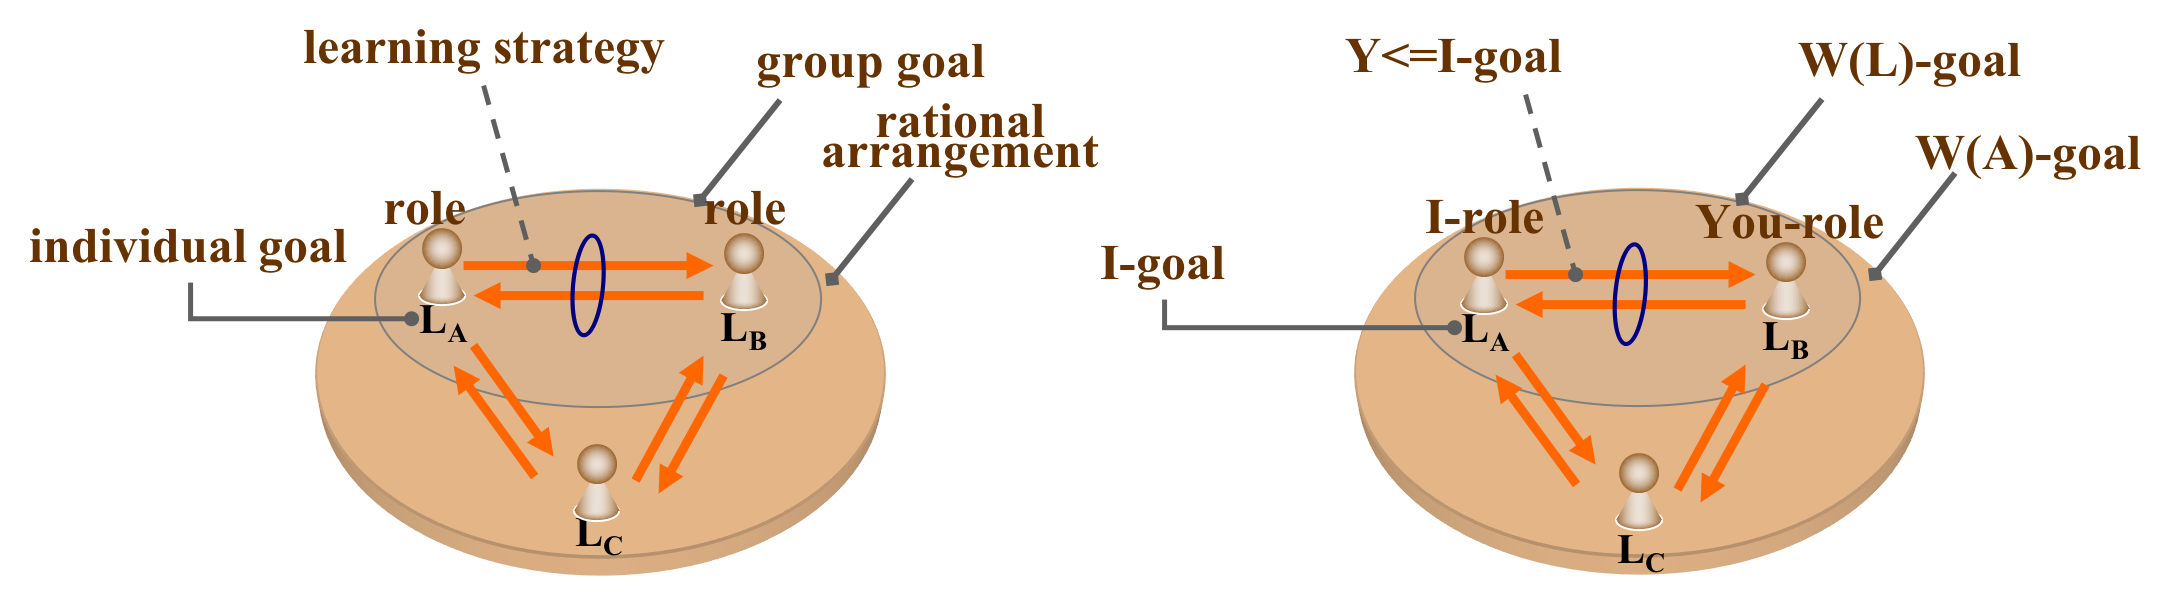
\includegraphics[width=0.95\textwidth]{images/chap-ontogacles1/concepts-terms-and-relation-in-cl-ontology.png}
 \fdireta{Isotani2009}
\end{figure}

To express the relationship of concepts described above, the CL Ontology employs the ontological structures shown in \autoref{fig:ontological-structure-cl-scenario} to represent CL scenarios. In these ontological structures, a CL scenario is represented by three parts defined as:  the \emph{Group structure benefit} (\emph{W(S)-goal}) to describe the expected benefits of the structured collaboration (i.e. positive interdependence, individual accountability, promotive interactions); the \emph{Learning strategy} (\emph{Y<=I-goal}) to describe the learning strategies employed by the group members in the CL scenario; and (3) the \emph{CL process} to describe the rational arrangement of the group activity (\emph{W(A)-goal}).

\begin{figure}[!htb]
 \caption{Ontological structure to represent CL scenarios}
 \label{fig:ontological-structure-cl-scenario}
 \centering
 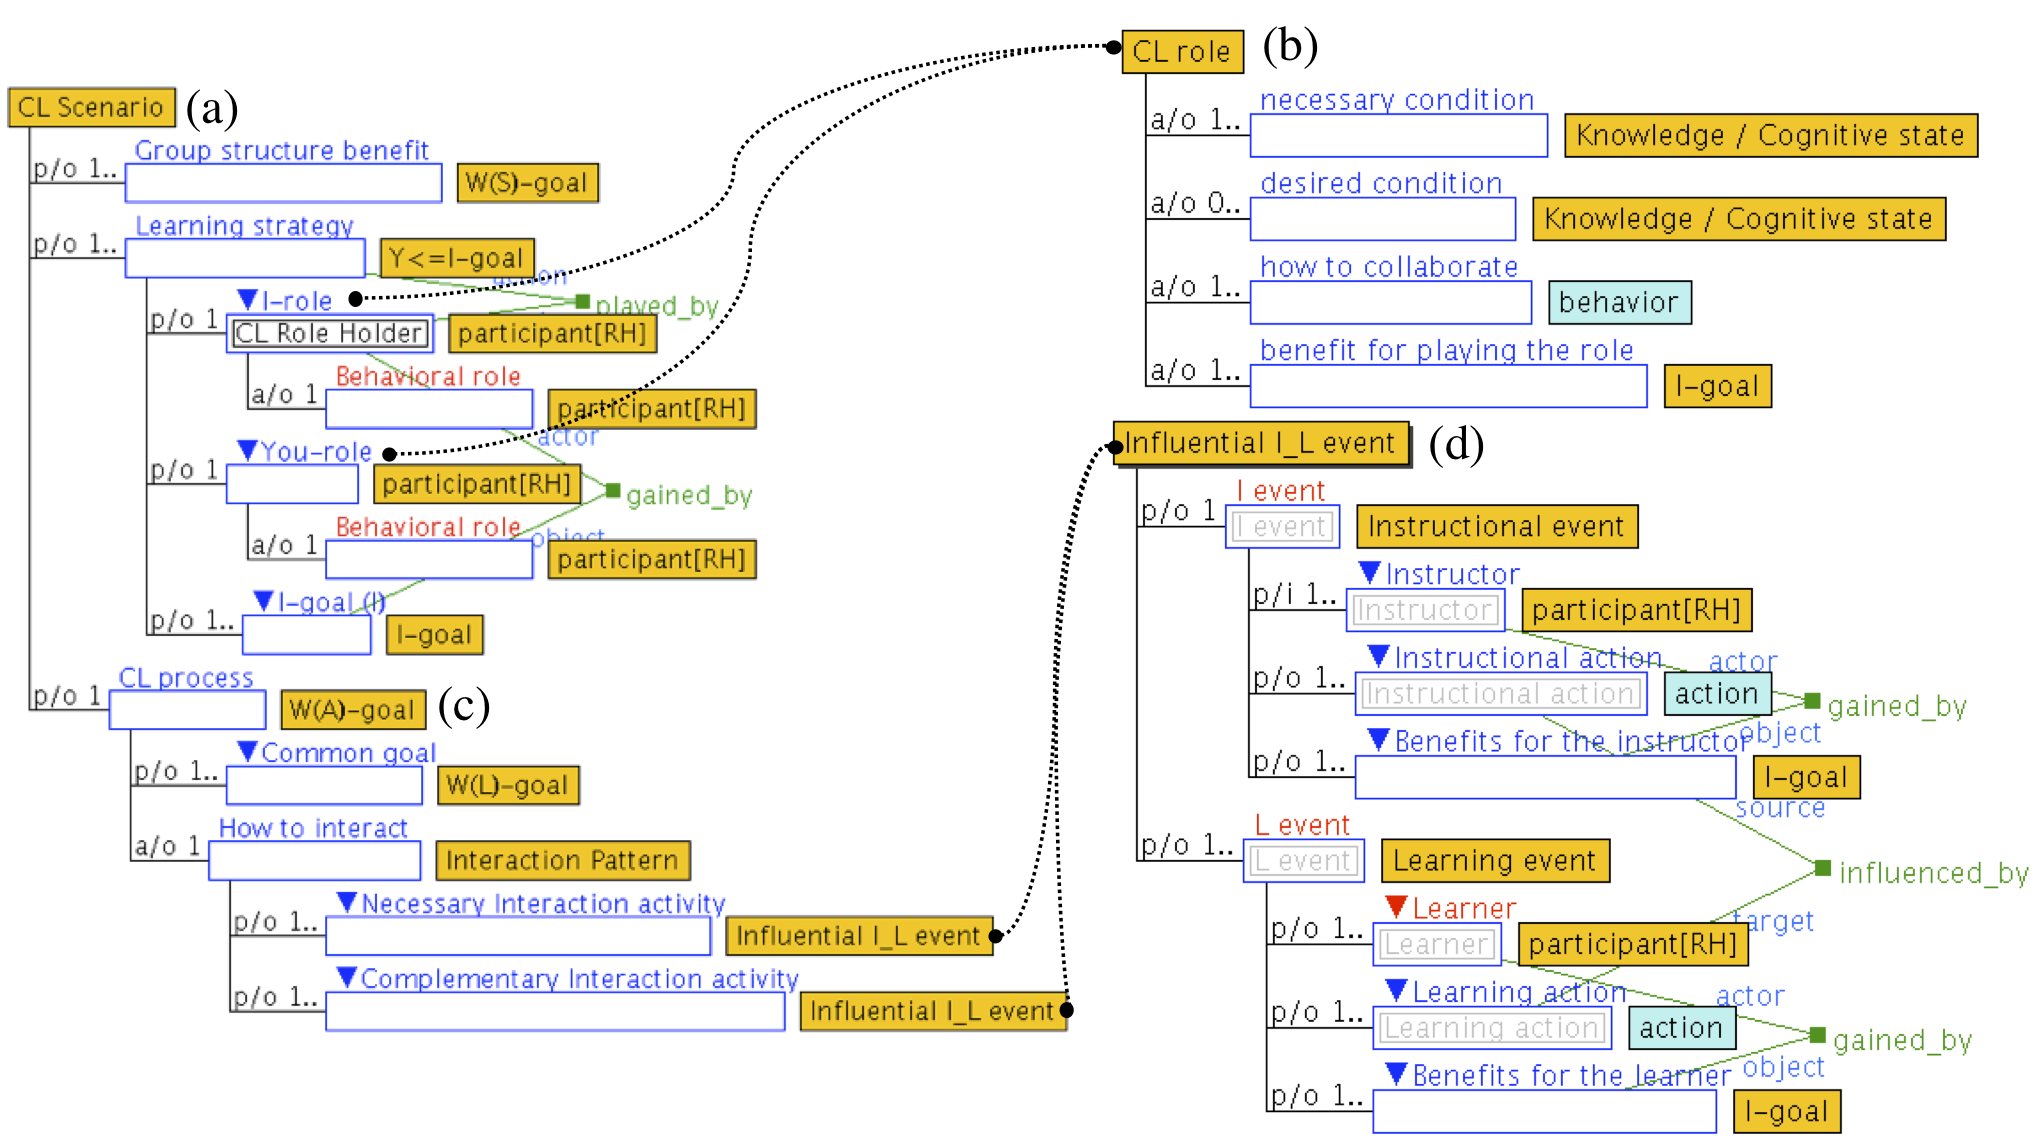
\includegraphics[width=1\textwidth]{images/chap-ontogacles1/ontological-structure-cl-scenario.png}
 \fdireta{Isotani2009}
\end{figure}

\begin{enumerate} [label=(\alph*)]

\item
The \textbf{Learning strategies} (\emph{Y<=I-goal}) are guidelines that specify how the participants should interact with others members of group to achieve their individual goals. These guidelines help the group members to externalize a desired behavior to play a given CL role more adequately. Therefore, the Learning strategy is represented as an ontological structure composes by: the participant in focus (\emph{I}) who plays the CL role \aspas{\emph{I-role}}, the participant (\emph{You}) who interacts with the participant in focus (\emph{I}) playing the CL role \aspas{\emph{You-role},} and the individual learning goals (\emph{I-goal}) that are expected to be achieved by the participant in focus (\emph{I}) at the end of CL scenario. The \emph{behavioral role} as part of the CL roles \aspas{\emph{I-role}} and \aspas{\emph{You-role}} is used to describe the behaviors externalized by the participants \aspas{\emph{I}} and \aspas{\emph{You}} when they interact in the CL scenario employing the learning strategy (\emph{Y<=I-goal}).

\item
The \textbf{CL role} describes functions, goals, duties and responsibilities that must be taken by members of group to achieve the common and individual learning goals. Thus, the ontological structure to represent a CL role is composed by: the \emph{necessary condition} and \emph{desired conditions} to play the CL role, the description of \emph{how to collaborate} when a group member plays the CL role, and the description of \emph{benefits for playing the role}. In this ontological structure, \emph{Cognitive/Knowledges states} are used to define the necessary and desired conditions for a group member to play the CL role, \emph{behaviors} are used to describe \emph{how to collaborate} playing the CL role, and individual learning goals (\emph{I-goal}) are employed to describe the expected \emph{benefits for playing the role}.

\item
The \textbf{CL process} is the \emph{rational arrangement of group activity} (\emph{W(A)-goal}) whereby the common and individual learning goals are achieved by the group members. This arrangement is represented by the \emph{common learning goals} (\emph{W(L)-goal}) as result of the negotiation process in the group formation, and by the \emph{Interaction Pattern} as the sequencing mechanism followed by the participants to achieve their individual learning goals (\emph{I-goal}). The interaction pattern is represented as a set of \emph{necessary} and \emph{desired interactions} in which the interaction for the group members is described as influential Instructional-Learning events (\emph{Influential I\_L events}).

\item
The \textbf{Influential I\_L event} represents the interaction among the group members and the benefits obtained by the interaction from two viewpoints: from the viewpoint of participants who play a role of instructor, and from the viewpoint of participants who play a role of learner. The influential I\_L event describes group members performing actions that influence other members with the purpose to change their own learning states by helping others to achieve their individual learning goals. Therefore, the ontological structure to represent an influential I\_L event is composed by two events: a \emph{learning event} and an \emph{instructional event} in which the participants are represented as actors of CL scenario playing CL roles and performing a set of actions to achieve their individual learning goals (\emph{I-goal}). For a group member acting as \emph{instructor}, the influential I\_L event describes his/her interaction with other group member who acts as \emph{learner} by means of instructional actions, and the expected \emph{benefits for the instructor} (\emph{I-goal}). For a group member acting as \emph{learner}, the influential I\_L event describes his/her interaction with other group member who acts as \emph{instructor} by means of learning actions, and the expected \emph{benefits for the learner} (\emph{I-goal}).
\end{enumerate}

As it was said before, the ontological structures shown in \autoref{fig:ontological-structure-cl-scenario} are used to describe CL scenarios that compliant with instructional and learning theories. To illustrate this, \autoref{fig:cognitive-apprenticeship-ontological-structure} shows the representation of a CL scenario based on the Cognitive Apprentice theory. According to this theory, the CL activities should incorporate situations that are familiar to those who are using these activities, and these situations must to lead the participants to act and interact acquiring skills in a specific context, and then generalizing these skills to other situations. Therefore, the CL scenarios based on the Cognitive Apprentice theory focuses on supporting a more skilled participant (known as \emph{master}) to teach a familiar situation for the lesser skilled participants (known as \emph{apprentices}) who learn by observing the skilled participant's behaviors and mimic him/her in other similar situations. From the viewpoint of the more skilled participant, he/she is supported by the learning strategy \aspas{\emph{learning by guiding}} (a1), his/her role (\emph{I-role}) is the \emph{Master role} with a behavioral role of \emph{Guider}, and his/her individual learning goals are the \emph{development of cognitive} or \emph{meta-cognitive skills} at the levels of \emph{Autonomous stage}. From the viewpoint of a lesser skilled participant, he/she is supported by the learning strategy \aspas{\emph{learning strategy by guiding}} (a2) to interact with the master, his/her role (\emph{I-role}) is the \emph{Apprentice role} with the behavioral role of \emph{Imitator}, and his/her individual goals are the \emph{development of cognitive} and/or \emph{meta-cognitive skills} at the levels of \emph{Cognitive stage} and \emph{Associative stage}.

\begin{figure}[!htbp]
 \caption{Ontological structures to represent a CL scenario based on the cognitive apprenticeship theory}
 \label{fig:cognitive-apprenticeship-ontological-structure}
 \centering
 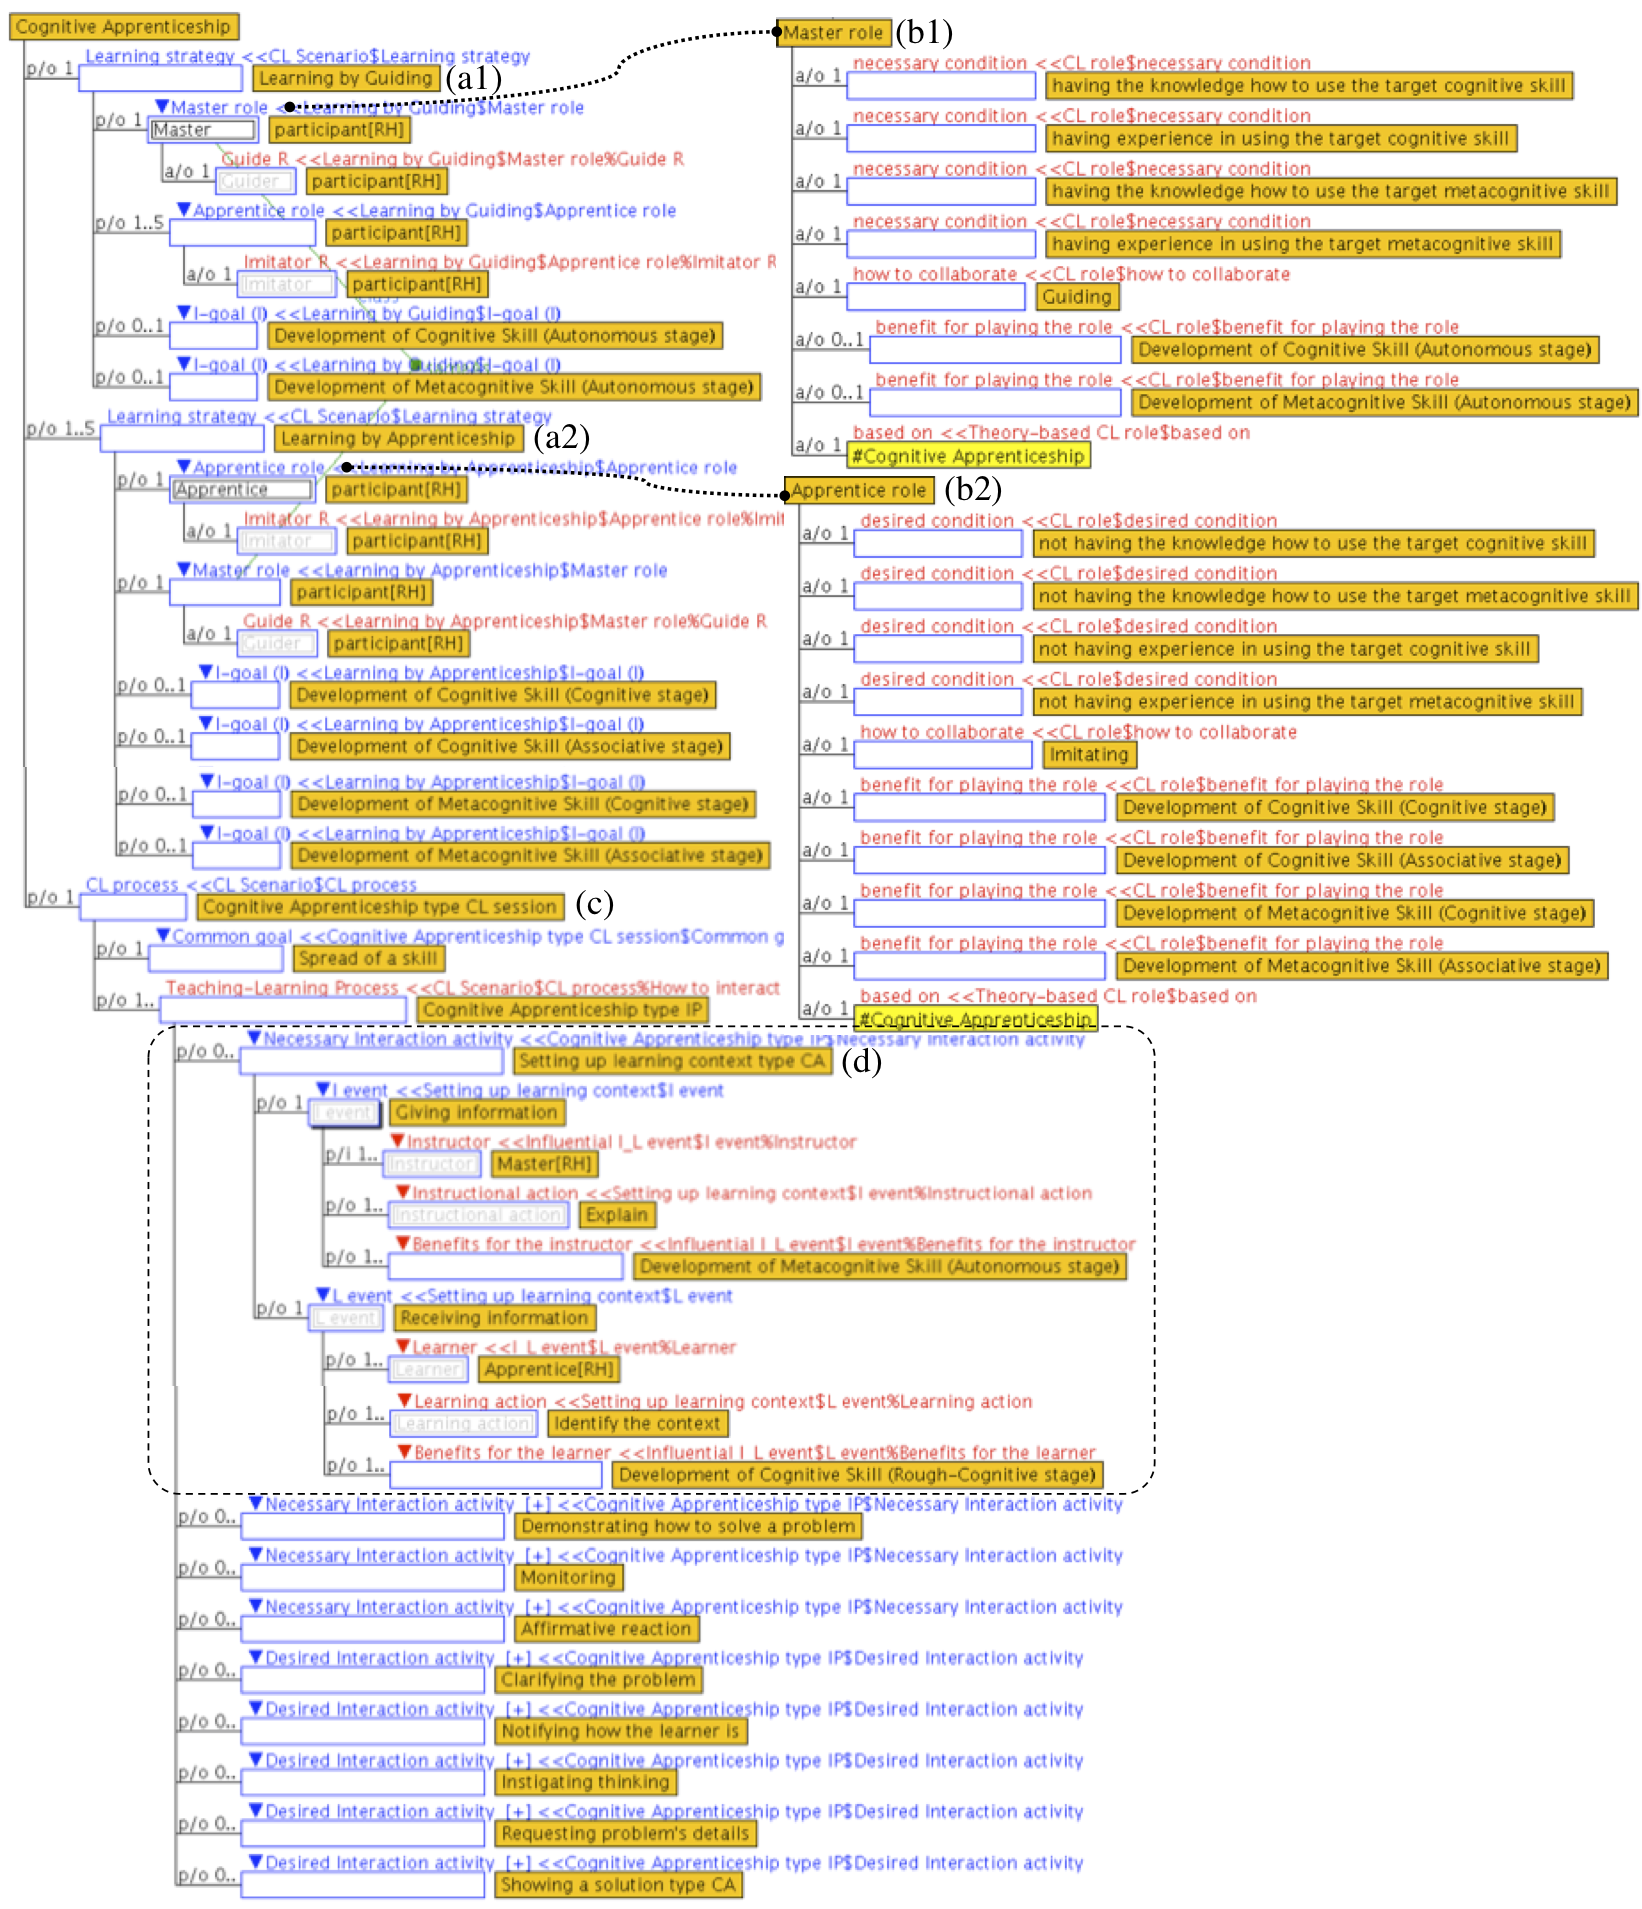
\includegraphics[width=1\textwidth]{images/chap-ontogacles1/cognitive-apprenticeship-ontological-structure.png}
 \fautor
\end{figure}

According to the cognitive apprentice theory, the more skilled participant who plays the master role must have knowledge and/or experience in using the target cognitive or metacognitive skill. Therefore, the necessary conditions to play the \emph{Master role} as shown in \autoref{fig:cognitive-apprenticeship-ontological-structure} (b1) are: \emph{having the knowledge how to use the target cognitive skill}, \emph{having experience in using the target cognitive skill}, and \emph{having experience in using the target metacognitive skill}.  When a participant adequately plays the master role, he/she acts \emph{Guiding} others participants, and as consequence of this behavior, he/she is benefited with the \emph{Development of cognitive or metacognitive skill} at the \emph{Autonomous stage}. The cognitive apprenticeship theory indicates that the participants without any knowledge or experience in how to use the target skill should play the apprentice role. Therefore, there is not necessary conditions in the ontological structure shown in \autoref{fig:cognitive-apprenticeship-ontological-structure} (b2) to represent the \emph{Apprentice role}, and the desired conditions for this role are: \emph{not having the knowledge how to use target metacognitive or cognitive skill} and \emph{not having experience in using the target metacognitive or cognitive skill}. When a participant adequately play the \emph{Apprentice role}, he/she acts \emph{Imitating} the behavior of the master and obtaining the benefits in the \emph{Development of metacognitive or cognitive skill} at the levels of \emph{Cognitive} and \emph{Associative} stages.

When the two learning strategies, \emph{Learning by Guiding} and \emph{Learning by Apprenticeship}, are simultaneously employed to structure the interactions among the participants in the CL scenario, a positive synergy is created among them producing a \emph{Spread of skills}. This arrangement is formalized by the ontological structure shown in \autoref{fig:cognitive-apprenticeship-ontological-structure} (c), where the \emph{CL process} is defined as a \emph{Cognitive Apprenticeship type CL session}, the \emph{Common goal} of this session is the \emph{Spread of skill}, and the \emph{Teaching-Learning Process} is an \emph{Interaction Pattern} defined by the sequencing mechanism of a CSCL script inspired by the Cognitive Apprenticeship theory. This sequencing mechanism defines the necessary and complementary interactions shown in \autoref{fig:cognitive-apprenticeship-cscl-script}. 

\begin{figure}[!htbp]
 \caption{Necessary and complementary interactions defined by the sequencing mechanism of a CSCL script inspired by the cognitive apprenticeship theory}
 \label{fig:cognitive-apprenticeship-cscl-script}
 \centering
 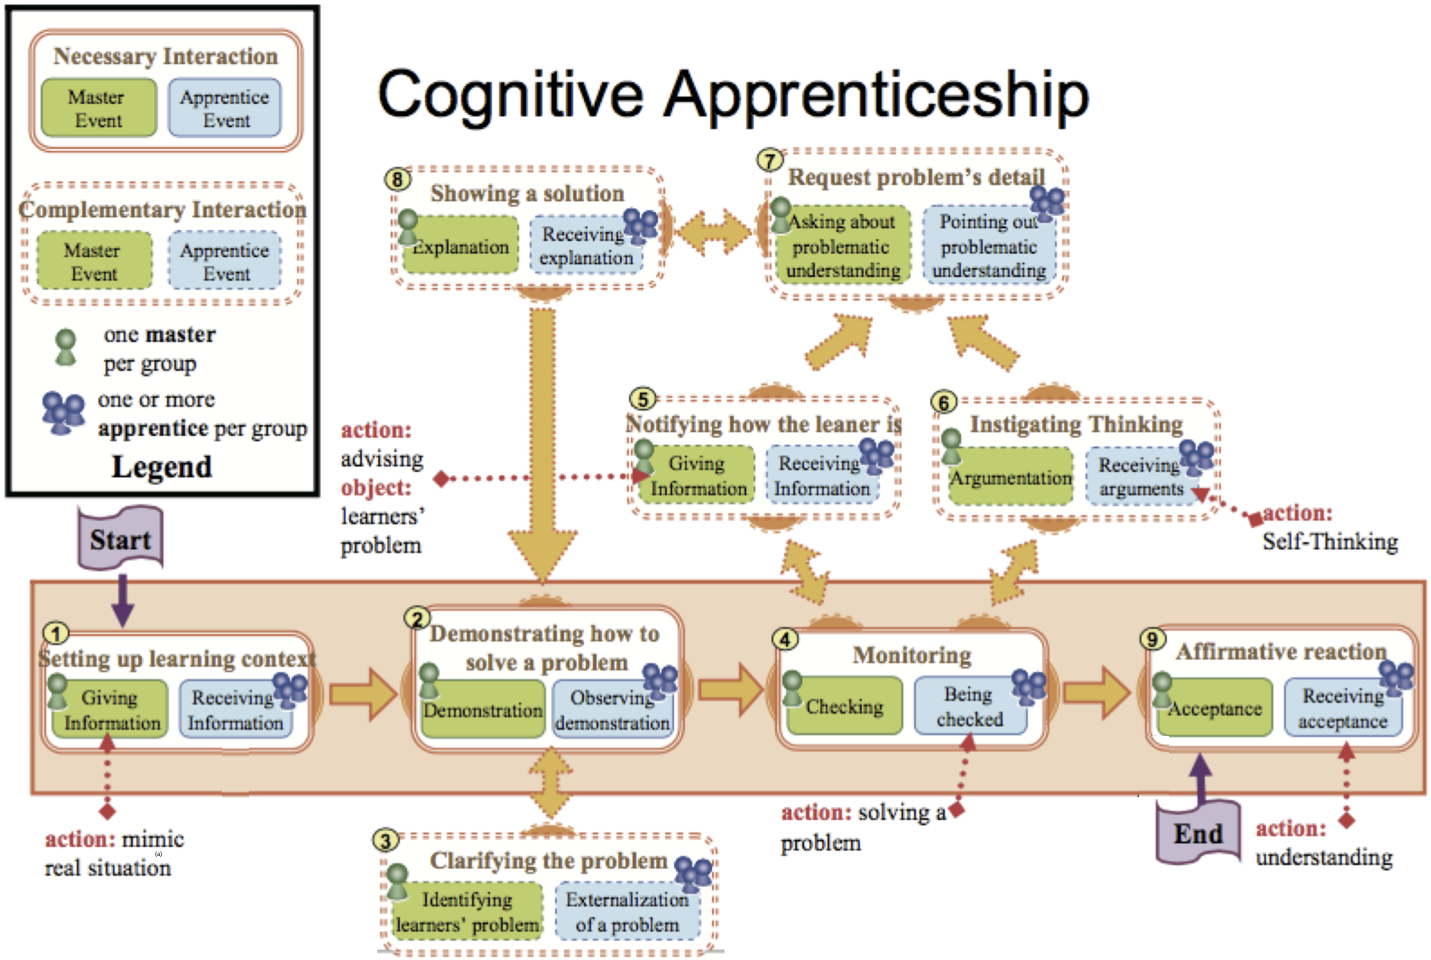
\includegraphics[width=1\textwidth]{images/chap-ontogacles1/cognitive-apprenticeship-cscl-script.png}
 \fadaptada{Isotani2009}
\end{figure}

The necessary and desired interactions defined by the sequencing mechanism shown in \autoref{fig:cognitive-apprenticeship-cscl-script} are formalized as \emph{Influential I\_L event} in the \emph{Teaching-Learning Process} of \emph{Cognitive Apprenticeship type CL session} shown in \autoref{fig:cognitive-apprenticeship-ontological-structure} (c). The ontological structure to represent the interaction \aspas{\emph{Setting up learning context type CA}} is shown in detail in \autoref{fig:cognitive-apprenticeship-ontological-structure} (d). In this interaction, the instructional event \aspas{\emph{Giving Information}} describes the action \aspas{\emph{Explain}} as an instructional action performed by the participant who plays the \emph{Master role} to \emph{develop the metacognitive skill} at the level of \emph{Autonomous stage}. The learning event \aspas{\emph{Receiving information}} describes the action \aspas{\emph{Identify the context}} as a learning action performed by the participant who plays the \emph{Apprentice role} to \emph{develop the cognitive skill} at the level of \emph{Rough-Cognitive stage}.


%%%%%%%%%%%%%%%%%%%%%%%%%%%%%%%%%%%%%%%%%%%%%%%%%%%%

\section[Ontological Structures to Represent Gamified CL Scenarios]{Ontological Structures to Represent Gamified Collaborative Learning Scenarios}
\label{sec:modeling-gamified-cl-scenarios}

The concepts, terms and relations shown in \autoref{fig:concepts-terms-and-relation-in-gamified-cl-scenarios} have been formalized in the ontology OntoGaCLeS to represent gamified CL scenarios. These elements employ an independent vocabulary from any theory and practice, and they are described as follows as:

\begin{figure}[!htbp]
 \caption{Concepts, terms and relations defined in the ontology to represent gamified CL scenarios}
 \label{fig:concepts-terms-and-relation-in-gamified-cl-scenarios}
 \centering
 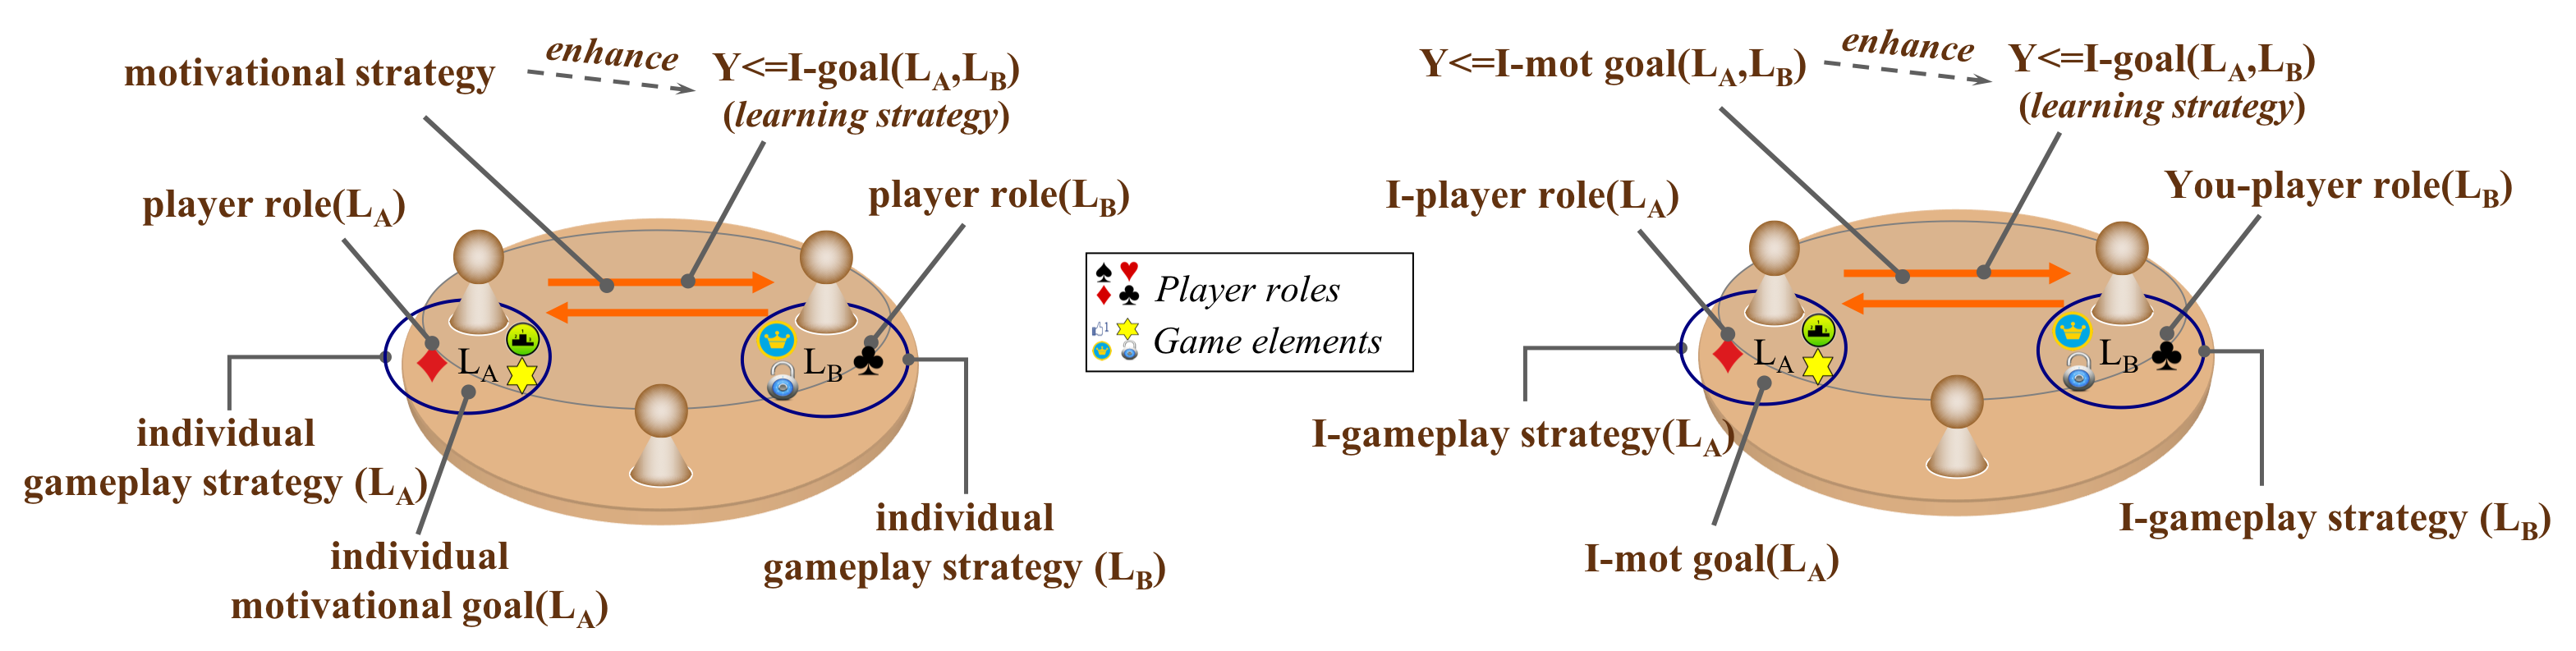
\includegraphics[width=1\textwidth]{images/chap-ontogacles1/concepts-terms-and-relation-in-gamified-cl-scenarios.png}
 \fautor
\end{figure}

\begin{description}
\item[\textbf{Y<=I-mot goal}]
is the \emph{individual motivational strategy} used to enhance the learning strategy (\emph{Y<=I-goal}) employed by the participant in focus (\emph{I}).

\item[\textbf{I-mot goal}]
is the \emph{individual motivational goal} for the participant in focus (\emph{I}), and it represents what is expected to happen in his/her motivational stage when an individual motivational strategy (\emph{Y<=I-mot goal}) is applied in the CL scenario to enhance the learning strategy (\emph{Y<=I-goal}) employed by him/her to interact with other member of group (\emph{You}).

\item[\textbf{I-player role}]
is the \emph{player role} for the participant in focus (\emph{I}).

\item[\textbf{You-player role}]
is the \emph{player role} for the participant (\emph{You}) who interacts with the participant in focus (\emph{I}).

\item[\textbf{I-gameplay}]
is the \emph{individual gameplay strategy} for the participant in focus (\emph{I}), and it describes the implementation of the individual motivational strategy (\emph{Y<=I-mot goal}) when this strategy corresponds to the gamification.
\end{description}

In the following subsections, the formalization of concepts, terms and relations briefly introduced here are detailed.

\subsection{Individual Motivational Goal (I-mot goal)}
\label{subsec:individual-motivational-goal}

The \emph{individual motivational goal} (\emph{I-mot goal}) has been formalized in the ontology OntoGaCLeS to represent the reason why is necessary to apply an individual motivational strategy in a CL scenario. Thus, for the participant in focus (\emph{I}), the individual motivational goal (\emph{I-mot goal}) represents what is expected to happen in his/her motivational stage when a motivational strategy is applied in the CL scenario to enhance the learning strategy employed by him/her to interact with others. In this sense, the individual motivational goal describes the motivational stages that must be reached by a person to be motivated to interact with other.

\autoref{fig:ontological-structure-i-mot-goal} shows the ontological structure that has been formalized in the ontology OntoGaCLeS to represent an individual motivational goal (\emph{I-mot goal}), where: the \emph{initial stage} and \emph{goal stage} are stages used to represent the expected change in the motivational stage of the person in focus (\emph{I}).

\begin{figure}[!htbp]
 \caption[Ontological structures to represent individual motivational goal (I-mot goal)]{Ontological structures to represent individual motivational goal (\emph{I-mot goal}). At the bottom, the \aspas{\emph{Satisfaction of psychological need}} (left) and the \aspas{\emph{Internalization of motivation}} (right)}
 \label{fig:ontological-structure-i-mot-goal}
 \centering
 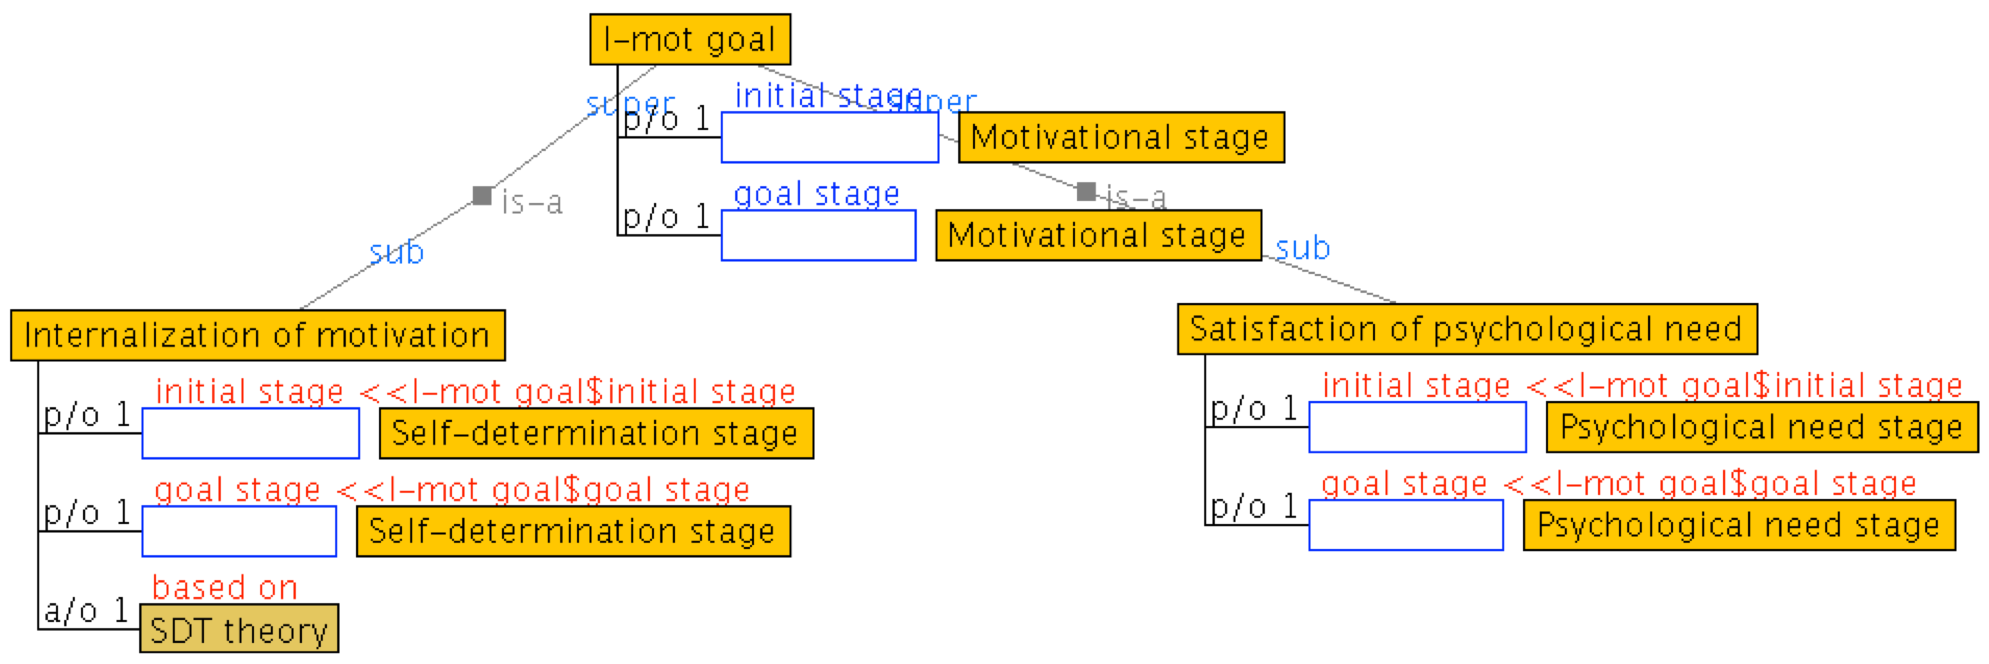
\includegraphics[width=1\textwidth]{images/chap-ontogacles1/ontological-structure-i-mot-goal.png}
 \fautor
\end{figure}

Two types of individual motivational goals have been currently formalized in the ontology OntoGaCLeS to describe the individual motivational goals (\emph{I-mot goal}) related to gamification as individual motivational strategy. The former, known as \emph{Satisfaction of psychological needs}, has been formalized based on the conceptualization of motivation as internal psychological process to satisfy human needs \cite{PritchardAshwood2008}; and the latter, known as \emph{Internalization of motivation}, has been formalized based on the form in which an individual regulates his/her own choices to behave and act \cite{DeciRyan2010}. \autoref{fig:ontological-structure-i-mot-goal} shows the representation for these two types of individual motivational goals. The initial and goal stages related to the \emph{Internalization of motivation} are defined by the self-determination stage, whereas the initial and goal stages for the \emph{Satisfaction of psychological need} are defined by the \emph{psychological need stages}. In the articles  \cite{ChallcoMoreiraBittencourtMizoguchiIsotani2015, ChallcoMoreiraMizoguchiIsotani2014, ChallcoMoreiraMizoguchiIsotani2014a}, the author of this thesis used the concept of \aspas{\emph{Phychological need}} to refer the concept of \aspas{\emph{Psychological need stage},} and the concept of \aspas{\emph{Without need}} to refer the stages described as \aspas{\emph{\$1 need satisfied}} where \$1 is substitute by psychological needs (e.g. \emph{Mastery need satisfied}).

As it was mentioned before, in the \autoref{chapter:general-background}, motivation is an internal psychological process associated with three general components of arousal, direction and intensity in which the arousal component is caused by needs (also called \emph{wants} or \emph{desires}). These needs cause that a person behaves and acts to satisfy needs \cite{MitchellDaniels2003}. Consequently, motivation is a constructor that describes why a person chooses to allocate time and energy for different behaviors and actions to maximize the satisfaction of his/her own needs \cite{PritchardAshwood2008}. It means that, in a CL scenario, the motivation problem caused by the scripted collaboration occurs when the participant believes that this scenario will not lead him/her to satisfy his/her individual needs. Therefore, the motivational strategy is applied in the CL scenario to change this perception. Based on this assumption, the individual motivational goals (\emph{I-mot goal}) for the person in focus (\emph{I}) has been formalized in the ontology OntoGaCLeS as the satisfaction of needs. More specifically, in gamified CL scenarios, the individual motivational goal is described as \emph{Satisfaction of psychological needs} because game elements do not satisfy all human needs, they only satisfy part of these needs that are referred by the author of this thesis as \emph{psychological needs}. The psychological needs are the human needs that are classified in the groups of relatedness and growth needs according to the ERG (Existence, Relatedness and Growth) theory \cite{Alderfer1972}.

\begin{figure}[!htbp]
 \caption[Ontological structures to represent satisfaction of psychological need]{Ontological structures to represent \aspas{\emph{Satisfaction of psychological need}.} At the top right, the ontological structure to represent \aspas{\emph{Satisfaction of autonomy}.}}
 \label{fig:ontological-structure-satisfaction-psychological-need}
 \centering
 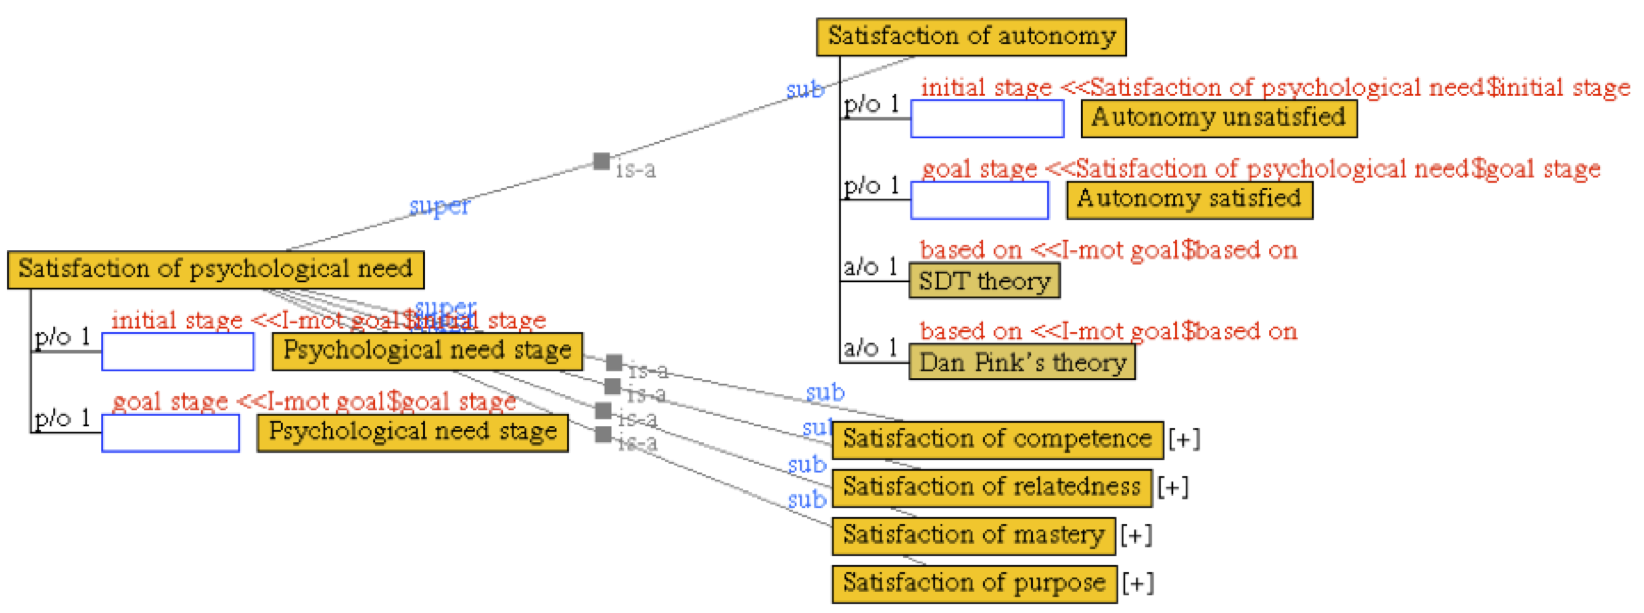
\includegraphics[width=1\textwidth]{images/chap-ontogacles1/ontological-structure-satisfaction-psychological-need.png}
 \fautor
\end{figure}

\autoref{fig:ontological-structure-satisfaction-psychological-need} shows the ontological structures formalized to represent the \emph{Satisfaction of psychological need}. These ontological structures represent the satisfaction of innate psychological needs, and they comprise what is intended to evoke in minds of users by the majority of experts when non-game contexts are gamified \cite{MoraRieraGonzalezArnedo-Moreno2015, SeabornFels2015}. According to the SDT theory \cite{RyanDeci2000,DeciRyan2010}, the well-being of an individual is reached when the psychological needs of autonomy, competence and relatedness are satisfied \cite{DeciRyan1985, DeciRyan2010}, and according to the Dan Pink's theory \cite{Pink2011}, a person is motivate and engage in a cognitive, decision-making, creative or higher-order thinking task when it is given with autonomy, mastery and purpose. At the top right of \autoref{fig:ontological-structure-satisfaction-psychological-need}, the ontological structure to represent the \emph{Satisfaction of autonomy} is detailed in which, based on a unipolar scale from unsatisfied need to satisfied need, the roles for the initial and goal stages are played by the \emph{Autonomy unsatisfied} and the \emph{Autonomy satisfied}, respectively. Employing the same unipolar scale, and the need-theories of motivation, SDT theory \cite{DeciRyan2010} and Dan Pink motivation theory \cite{Pink2011}, a set of individual motivational goals as satisfactions of psychological needs have been formalized in the ontology OntoGaCLeS, and they are detailed in \autoref{sec:ontogacles:i-mot-goal}.

\begin{figure}[!htbp]
 \caption[Ontological structures to represent internalization of motivation]{Ontological structures to represent \aspas{\emph{Internalization of motivation}.} At the top right, the ontological structure to represent the \aspas{\emph{Internalization from amotivation to intrinsic motion}.}}
 \label{fig:ontological-structure-internalization-motivation}
 \centering
 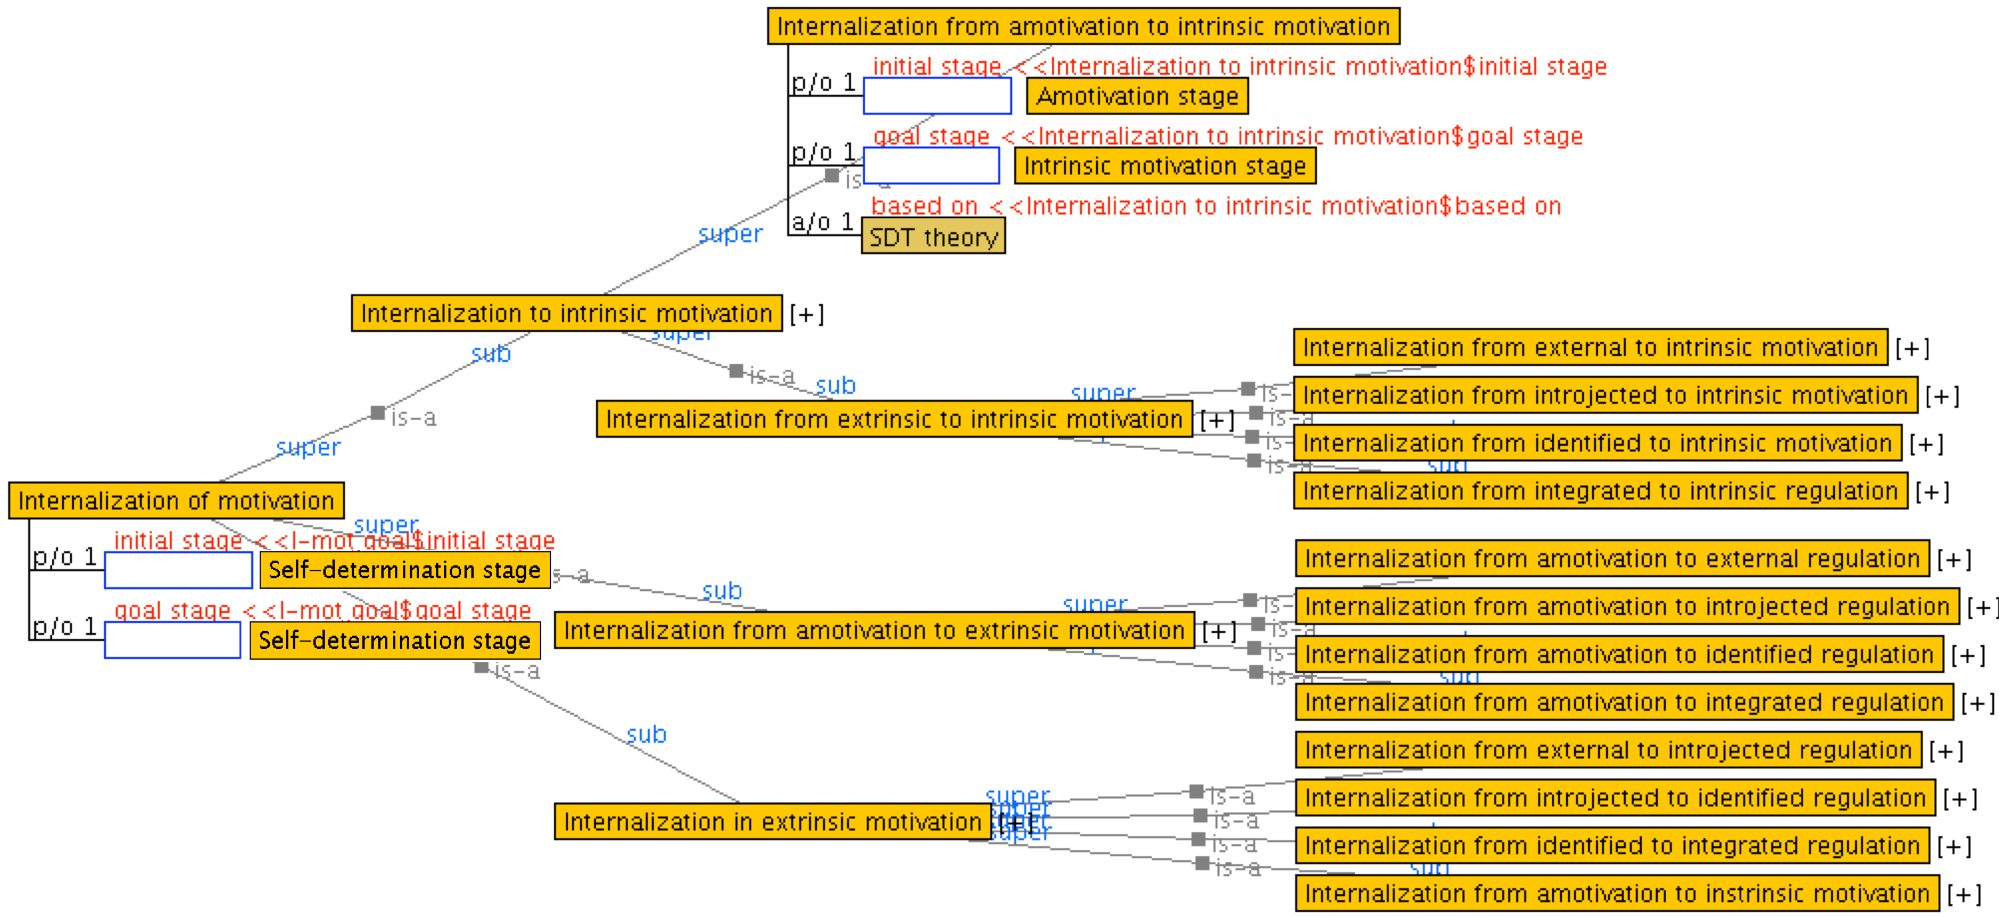
\includegraphics[width=1\textwidth]{images/chap-ontogacles1/ontological-structure-internalization-motivation.png}
 \fautor
\end{figure}

The \emph{internalization of motivation} is the process by which \aspas{\emph{values, attitudes or regulatory structures, such that the external regulation of a behavior is transformed into an internal regulation, so no longer requires the presence of an external contingency}} \cite{GagneDeci2005}. In this sense, the internalization of motivation in relation to the satisfaction of needs refers to changes in the motivation from a non-free choice to a free choice of needs that are satisfied by oneself. According to the SDT theory \cite{DeciRyan1985, RyanDeci2000}, this change happens from the extrinsic motivation to intrinsic motivation when motivation is changed from a non-self-determined form (\emph{non-freely choice}) to a self-determined form (\emph{freely choice by oneself}). Here, the extrinsic motivators employed by the game elements must be configured as an attempt to transform the current motivation stages of participants from amotivation and extrinsic motivation into intrinsic motivation. Based on these definitions, the ontological structures shown in \autoref{fig:ontological-structure-internalization-motivation} have been formalized in the ontology OntoGaCLeS to represent the \emph{Internalization of motivation}. These ontological structures have been formalized employing the continuum ranging of stages from \emph{amotivation} (not internalized behave) into \emph{external motivation} (not at all internalized behave) to \emph{introjected motivation} (partially internalized behave) to \emph{identified motivation} (fully internalized behave) to \emph{intrinsic motivation} (automatically internalized behave). At the top right of \autoref{fig:ontological-structure-internalization-motivation} is detailed the formalization for the change from \emph{Amotivation stage} (\emph{initial stage}) to \emph{Intrinsic motivation stage} (\emph{goal stage}) defined as \aspas{\emph{Internalization from amotivation to intrinsic motivation}.} The detailing of all ontological structures to represent the internalization of motivation is presented in \autoref{sec:ontogacles:i-mot-goal}.

\subsection{Player Role}
\label{subsec:player-role}

The identification of homogeneous people groups that differ from other groups in a significant way is essential to define the personalization in any system. In game design, this segmentation is established by player types models in which typologies are used to categorize the users in different groups according to their geographic location \cite{BenJuddChrisAvelloneHideoKojimaKeijiInafune2016, ChakrabortyNorcioVeerAndreMillerRegelsberger2015}, their demographic situation \cite{GreenbergSherryLachlanLucasHolmstrom2010, Shaw2012}, their psychographic characteristics \cite{Tseng2011, Yee2006}, and their behavioral characteristics \cite{Bartle2004, Lazzaro2009}. These player type models aim to help the game designers to identify the necessary features that make a game fun, enjoyable and desirable for a particular audience.

The player type models cannot be directly extrapolated to others context for which they are not intended. Thus, the concept of \emph{Player role} has been formalized by the author of this thesis in the ontology OntoGaCLeS to define typologies of player types in the context of CL scenarios. Player roles describe the functionality, responsibilities and requirements whereby a group of participants becomes players in a gamified CL scenario. This segmentation is based on individual characteristics of participants that establish a segmentation of participants using necessary and desired conditions. In this sense, the \emph{Player role} has been formalized by the ontological structure shown in \autoref{fig:ontological-structure-player-role}. This structure defines the conditions that must be satisfied by a participant in the CL scenario to play the player role as: \emph{necessary condition} and \emph{desired condition}. Thus, a participant of CL scenario cannot play a player role when he/she does not fulfill the necessary conditions, and when the participant fulfills the necessary and desired conditions has more probability to obtain the expected \emph{benefits for playing the role}.

The necessary and desire conditions in the ontological structure to represent \emph{Player role} are defined by: motivation states, psychological need states, and individual personality trait states. A tree overview for these states are detailed in \autoref{sec:ontogacles:tree-overview-states}, where:

\begin{itemize}
\item
The \emph{motivation state} is an internal state that describes the temporal attitudinal state of a person in relation to his/her desire to be a participant in the CL session. These stages can be \emph{Not motivated} and \emph{Motivated}. The state of motivated is also divided in two types: \aspas{\emph{Intrinsic motivated}} and \aspas{\emph{Extrinsic motivated}} \cite{DeciRyan2010}. It is important to notice here that the concept of motivation state is not the same as the concept of motivation stage. Although both concepts represent changes in relation to the motivation of participants, the motivation state represents a specific point in the whole process of being motivated, whereas the motivation stage represents an interval in the motivation process.

\item
The \emph{psychological need state} represents the current psychological need of a person in which the states for each one of the psychological needs are formalized through the representation of pair states: \aspas{\emph{Having need of \$1}} and \aspas{\emph{Not having need of \$1}} in which \aspas{\emph{\$1}} is replaced by the name of the need that is being described as prerequisite. For instance, to represent the states related to the psychological need of competence, the states of \aspas{\emph{Having need of competence}} and \aspas{\emph{Not having need of competence}} have been formalized as psychological need state in the ontology OntoGaCLeS.

\item
The \emph{individual personality trait state} describes states related to individual personality traits, such as introversion, extraversion, openness to experience, and conscientiousness. The individual personality trait states describe the characteristic that make a person unique by indicating his/her habitual patterns of thought, emotion and behavior for different situations \cite{MatthewsDearyWhiteman2003}. These states express whether a participant either has or does not have the individual personality trait. In the ontology OntoGaCLeS, there are represented individual personality traits states related to: the big five personality traits \cite{CostaMacCrae1992}, the MBTI personality traits \cite{Briggs1976}, the game-playing style preferences described in the Bartle's player type model \cite{Bartle2004}, and the game-playing liking preferences described in the Yee's motivation components \cite{Yee2006}.
\end{itemize}

\begin{figure}[!htbp]
 \caption[Ontological structure to represent player role]{Ontological structure to represent \aspas{\emph{Player role}} (At the top). At the bottom, the ontological structure to represent the player role \aspas{\emph{Dreamer role}.}}
 \label{fig:ontological-structure-player-role}
 \centering
 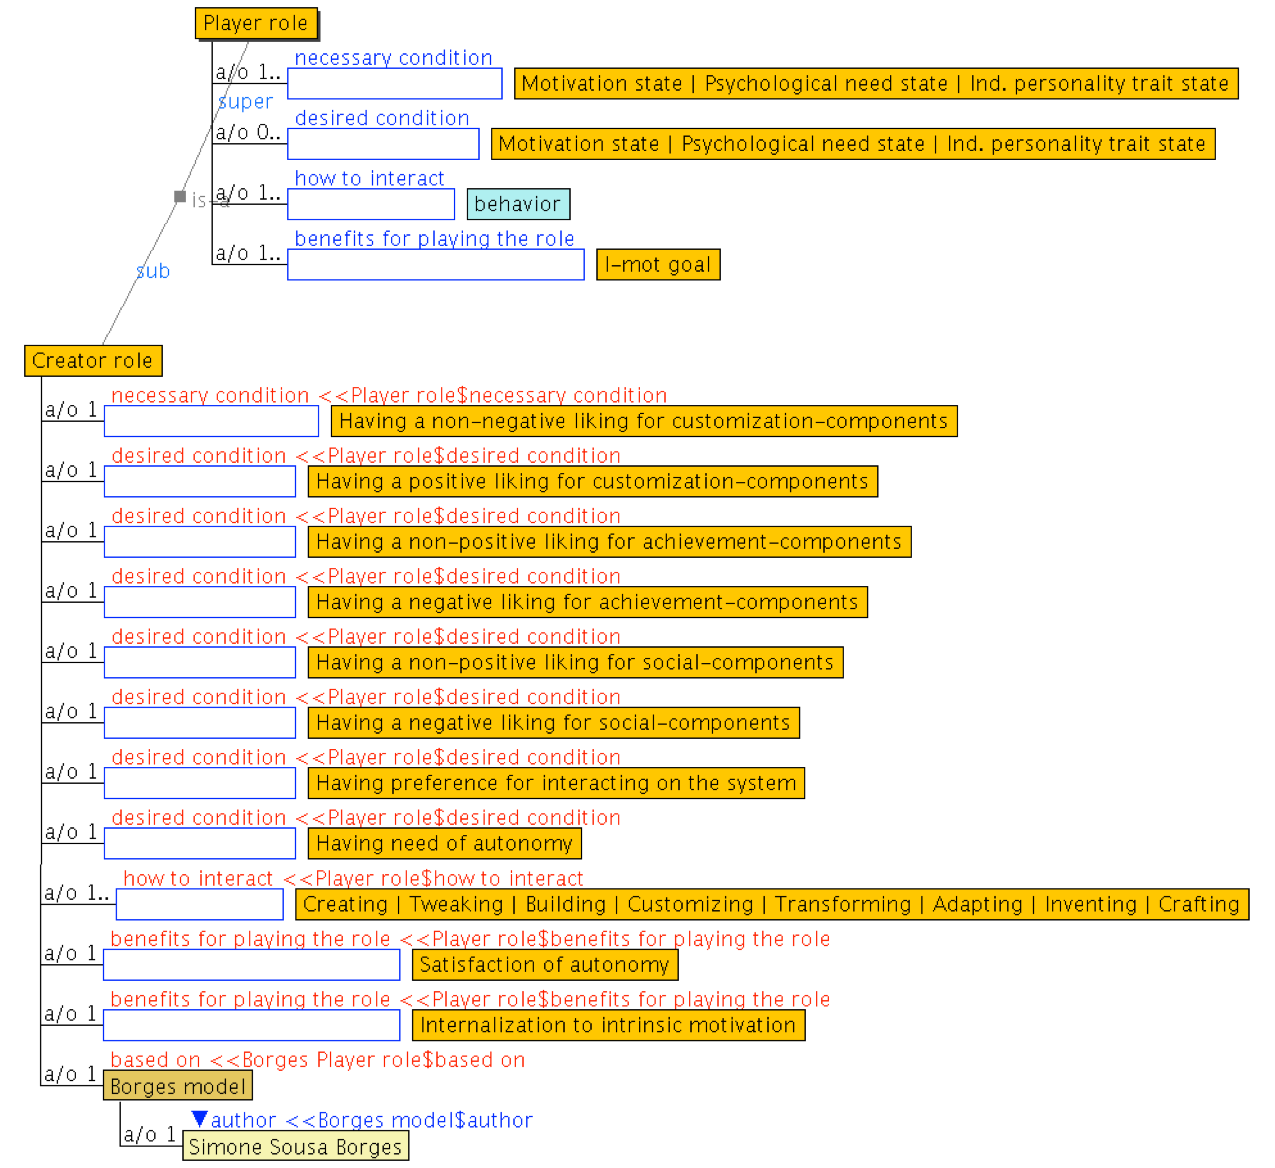
\includegraphics[width=1\textwidth]{images/chap-ontogacles1/ontological-structure-player-role.png}
 \fautor
\end{figure}

Beside to describe the necessary and desired conditions that should be satisfied by an individual, the ontological structure to represent \emph{Player role} shown in \autoref{fig:ontological-structure-player-role} describe the information about: how the participant with the player role is expected to interact with the game elements (\emph{how to interact}), and the expected benefits for playing the player role (\emph{benefits for playing the role}). Thus, concepts described as \emph{behavior} are used to represent the possible manners in which a participant should interact to other, and concepts described as individual motivational goals (\emph{I-mot goal}) are used to represent the expected \emph{benefits for playing the role}.

At the bottom of \autoref{fig:ontological-structure-player-role}, the \emph{Creator role} is shown as example of the formalization of a player role using the ontological structure proposed in this section. According to this structure, participants who have a greater liking for customization-components rather than for other game components are classified as creators. This segmentation is represented by the necessary condition of \aspas{\emph{having a non-negative liking for customization-components},} and the desired conditions of \aspas{\emph{having a positive liking for customization-components},} \aspas{\emph{having a non-positive liking for achievement-component},} \aspas{\emph{having a negative liking for achievement-component},} \aspas{\emph{having a non-positive liking for social-component},} and \aspas{\emph{having a negative liking for social-component}.} The desired conditions related to the behavioral characteristics of participants to act as a player role are: \aspas{\emph{having preference for interacting on the system}} and \aspas{\emph{having need of autonomy}.} The expected behaviors to obtain benefits for playing the creator role are: \aspas{\emph{Creating},} \aspas{\emph{Tweaking},} \aspas{\emph{Building},} \aspas{\emph{Customizing},} \aspas{\emph{Transforming},} \aspas{\emph{Adapting},} \aspas{\emph{Inventing}} or \aspas{\emph{Crafting}.} As consequence to behave as creator, the participants attain the \emph{Satisfaction of autonomy} and the \emph{Internalization to intrinsic motivation} (\emph{I-mot goal}).

In the ontology OntoGaCLeS, based on the information extracted from five different player type models, twenty-six players roles have been formalized and represented using the ontological structure proposed in this section. These player roles, their conditions, expected behaviors and benefits for the person who plays the role are detailed in \autoref{sec:ontogacles:player-role}.

\subsection{Individual Motivational Strategy (Y<=I-mot goal)}

In the context of CL scenarios, an \emph{individual motivational strategy} is defined by the author of this thesis as a set of guidelines defined to motivate a participant to interact with other group members using learning strategies. These guidelines are independent of any technology, so that the individual motivational strategy basically describes what motivates a participant to act and behave in certain way. For example, consider the following guidelines extracted from the Model-driven Persuasive Game in which:

\begin{citacao}
\aspas{... cooperation is only a significant motivator of behaviour change for achievers and socializers... This is in line with the gaming style of socializers, who enjoy helping others. Achievers would also prefer to cooperate because they are inherently more altruistic ... achievers do often co-operate with one another, usually to perform some difficult collective goal, and from these shared experiences can grow deep, enduring friendships which may surpass in intensity those commonly found among individuals other groups.} \citeonline{Orji2014}.
\end{citacao}

When these two guidelines are applied in a CL scenario by providing a situation in which the participants must cooperate to achieve a group goal (e.g. obtain a especial reward based on the collective performance of group members), these guidelines becomes a individual motivational strategy that could be applied to motivate participant who fall in the category of socializer or achiever because they are motivated by the desired to accomplish the group goal and the desired to help others, respectively.

The ontological structure shown in \autoref{fig:ontological-structure-individual-motivational-strategy} has been proposed by the author of this PhD thesis dissertation to represent the formalization of individual motivational strategies whose guidelines are extracted from gamification models or game design models. According to this structure, an \emph{individual motivational strategy} (\emph{Y<=I-mot goal}) is described by:

\begin{description}
\item[\textbf{I-player role}]
to indicate the player role for the participant in focus (\emph{I}) who becomes a \emph{player role holder} when he/she is motivated by the motivational strategy. This player role also indicates the \emph{behavioral roles} whereby the participant in focus (\emph{I}) is motivated to interact with other participant (\emph{You}) employing the learning strategy (\emph{Y<=I-goal}).

\item[\textbf{You-player role}]
to indicate the player role for the participant (\emph{You}) who interacts with the participant in focus (\emph{I}). The \emph{behavioral roles} whereby the \emph{player role holder} of this role supports the interaction of participant in focus (\emph{I}) are also indicated in this structure.

\item[\textbf{I-mot goal (I)}]
to indicate the individual motivational goals (\emph{I-mot goal (I)}) whereby the participant in focus (\emph{I}) is motivated to interact with other participant (\emph{You}) employing a learning strategy (\emph{Y<=I-goal}). In this sense, these individual motivational goals represent the reasons why the guidelines contained in the motivational strategy are applied in the CL scenario to enhance the learning strategy (\emph{Y<=I-goal}) employed by the participant in focus (\emph{I}) to interact with other participant (\emph{You}).
\end{description}

\begin{figure}[!htbp]
 \caption[Ontological structure to represent individual motivational strategy]{Ontological structure to represent \aspas{\emph{Individual motivational strategy}} (at the left). At the right, the motivational strategies \aspas{\emph{Gamifying for Consumer and Dodecad Achiever}} (right-top) and \aspas{\emph{Gamifying by COOP}} (right-bottom).}
 \label{fig:ontological-structure-individual-motivational-strategy}
 \centering
 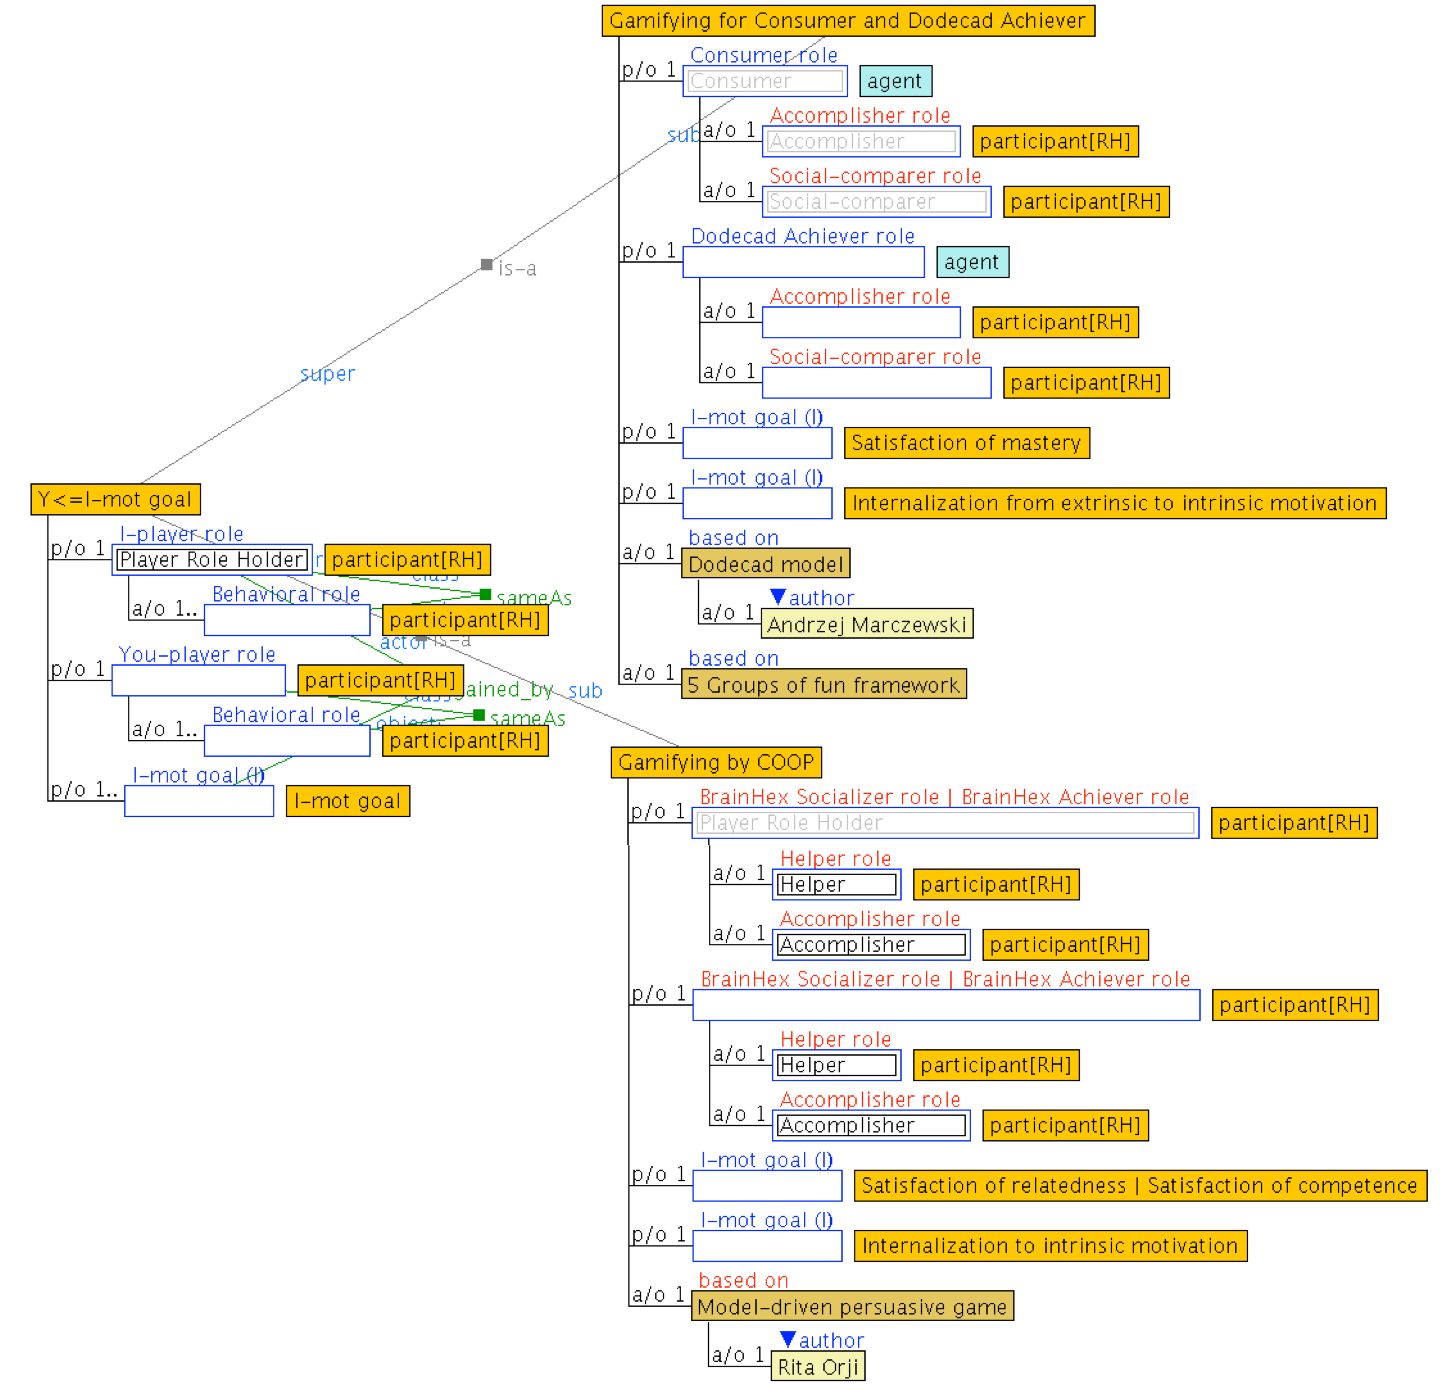
\includegraphics[width=1\textwidth]{images/chap-ontogacles1/ontological-structure-individual-motivational-strategy.png}
 \fautor
\end{figure}

To exemplify the formalization of the individual motivational strategies using the ontological structure proposed in this section, \autoref{fig:ontological-structure-individual-motivational-strategy} also shows two examples in which the attribute \aspas{\emph{based on}} indicates the gamification models in which these motivational strategies are based. The individual motivational strategy shown at the top-right of \autoref{fig:ontological-structure-individual-motivational-strategy} is known as \aspas{\emph{Gamifying for Consumer and Dodecad Achiever},} and it has been formalized based on guidelines of the Dodecad model \cite{Marczewski2015a} and 5 Groups of fun framework \cite{Marczewski2015b}. According to these guidelines, the consumers and achievers are motivated by the need to obtain a reward that demonstrates for other participants their accomplishments. Hence, the \emph{Accomplisher} and \emph{Social-comparer} are \emph{behavioral roles} whereby a participant in focus (\emph{I}) playing the \emph{Consumer role} is motivated to interact with the participant (\emph{You}) who plays the \emph{Achieve role}. Playing this role, the \emph{Satisfaction of mastery} and the \emph{Internalization from extrinsic to intrinsic motivation} are individual motivational goals whereby the participant in focus (\emph{I}) as consumer is motivated to interact with other participant (\emph{You}) who acts as achiever. Behaving as accomplisher and social-comparer, the participant in focus (\emph{I}) has two individual motivational goals that are: to demonstrate his/her mastery represented as \aspas{\emph{Satisfaction of mastery};} and to internalize his/her current extrinsic motivation stage into intrinsic motivation stage represented as \aspas{\emph{Internalization from extrinsic to intrinsic motivation}.}

At the bottom-right of \autoref{fig:ontological-structure-individual-motivational-strategy}, it is shown the ontological structure formalized to represent the application of the guidelines described in the Model-driven persuasive game for the cooperation strategy \cite{OrjiVassilevaMandryk2014}. These guidelines indicate cooperation as significant motivator for a participant who plays the socializer or achiever role because a participant who plays these roles enjoys to help others and cooperate with others in order to accomplish a difficult collective goal. Based on this, the motivational strategy of \aspas{\emph{Gamifying by COOP}} defines the \emph{BrainHex Socializer role} and \emph{Brainhex Achiever role} as player roles that would be played by the participant in focus (\emph{I}) and the participant (\emph{You}) who gives support to the participant in focus. Playing these roles, the participants (\emph{I} and \emph{You}) act as \emph{Helper} and \emph{Accomplisher}. When the participant in focus (\emph{I}) has the desire to accomplish the difficult collective goal, his/her individual motivational goal is the \emph{Satisfaction of competence}, and when the participant in focus (\emph{I}) has the desire to help others, his individual motivational goal is the \emph{Satisfaction of relatedness}. The ontological structure also describes that as consequence of the application of the motivational strategy, it is expected changes in the motivational state for the participant in focus (\emph{I}) from the amotivation or extrinsic motivated state to the intrinsic motivated state (\emph{Internalization to intrinsic motivation}).

The individual motivational strategies based on gamification models currently defined in the ontology OntoGaCLeS, their player roles, their behavioral roles, and their individual motivational goals are detailed in \autoref{sec:ontogacles:individual-motivational-strategy}.

\subsection{Individual Gameplay Strategy (I-gameplay strategy)}
\label{sec:individual-gameplay-strategy}

The guidelines extracted from the literature of gamification, game design and serious games are implemented through the design of way in which the users will experience their interactions with the game-like system \cite{FabricatoreLopez2014, NackeDrachenG"obel2010, Schell2008}. Such design in gamification is frequently called as gameful design \cite{DeterdingDixonKhaledNacke2011, DichevDichevaAngelovaAgre2014}, and it has been formalized by the author of this thesis under the concept of \emph{individual gameplay strategy} (\emph{I-gameplay strategy}). In this sense, the gameplay of a gamified CL scenario is defined by the way in which the interactions between the participants and the game elements could occur. When a participant interacts with the game elements, the rules defined in the gamified CL scenario process his/her inputs causing changes in the game elements, and these modifications are communicated to the participant. These rules and changes are related to individual motivational goals that must be achieved by the participants, so that each participant has his/her own strategy to interact with the gamified CL scenario to achieve these goals. This strategy of interaction is the individual gameplay strategy, and it has been formalized by the ontological structure shown in \autoref{fig:ontological-structure-individual-gameplay-strategy}.

\begin{figure}[!htbp]
 \caption[Ontological structure to represent individual gameplay strategy]{Ontological structure to represent \aspas{\emph{Individual gameplay strategy}} (at the top). At the bottom, the \aspas{\emph{Coop. CMPT gameplay strategy}} (bottom-left), and the \aspas{\emph{Achievement fun gameplay strategy}} (bottom-right)}
 \label{fig:ontological-structure-individual-gameplay-strategy}
 \centering
 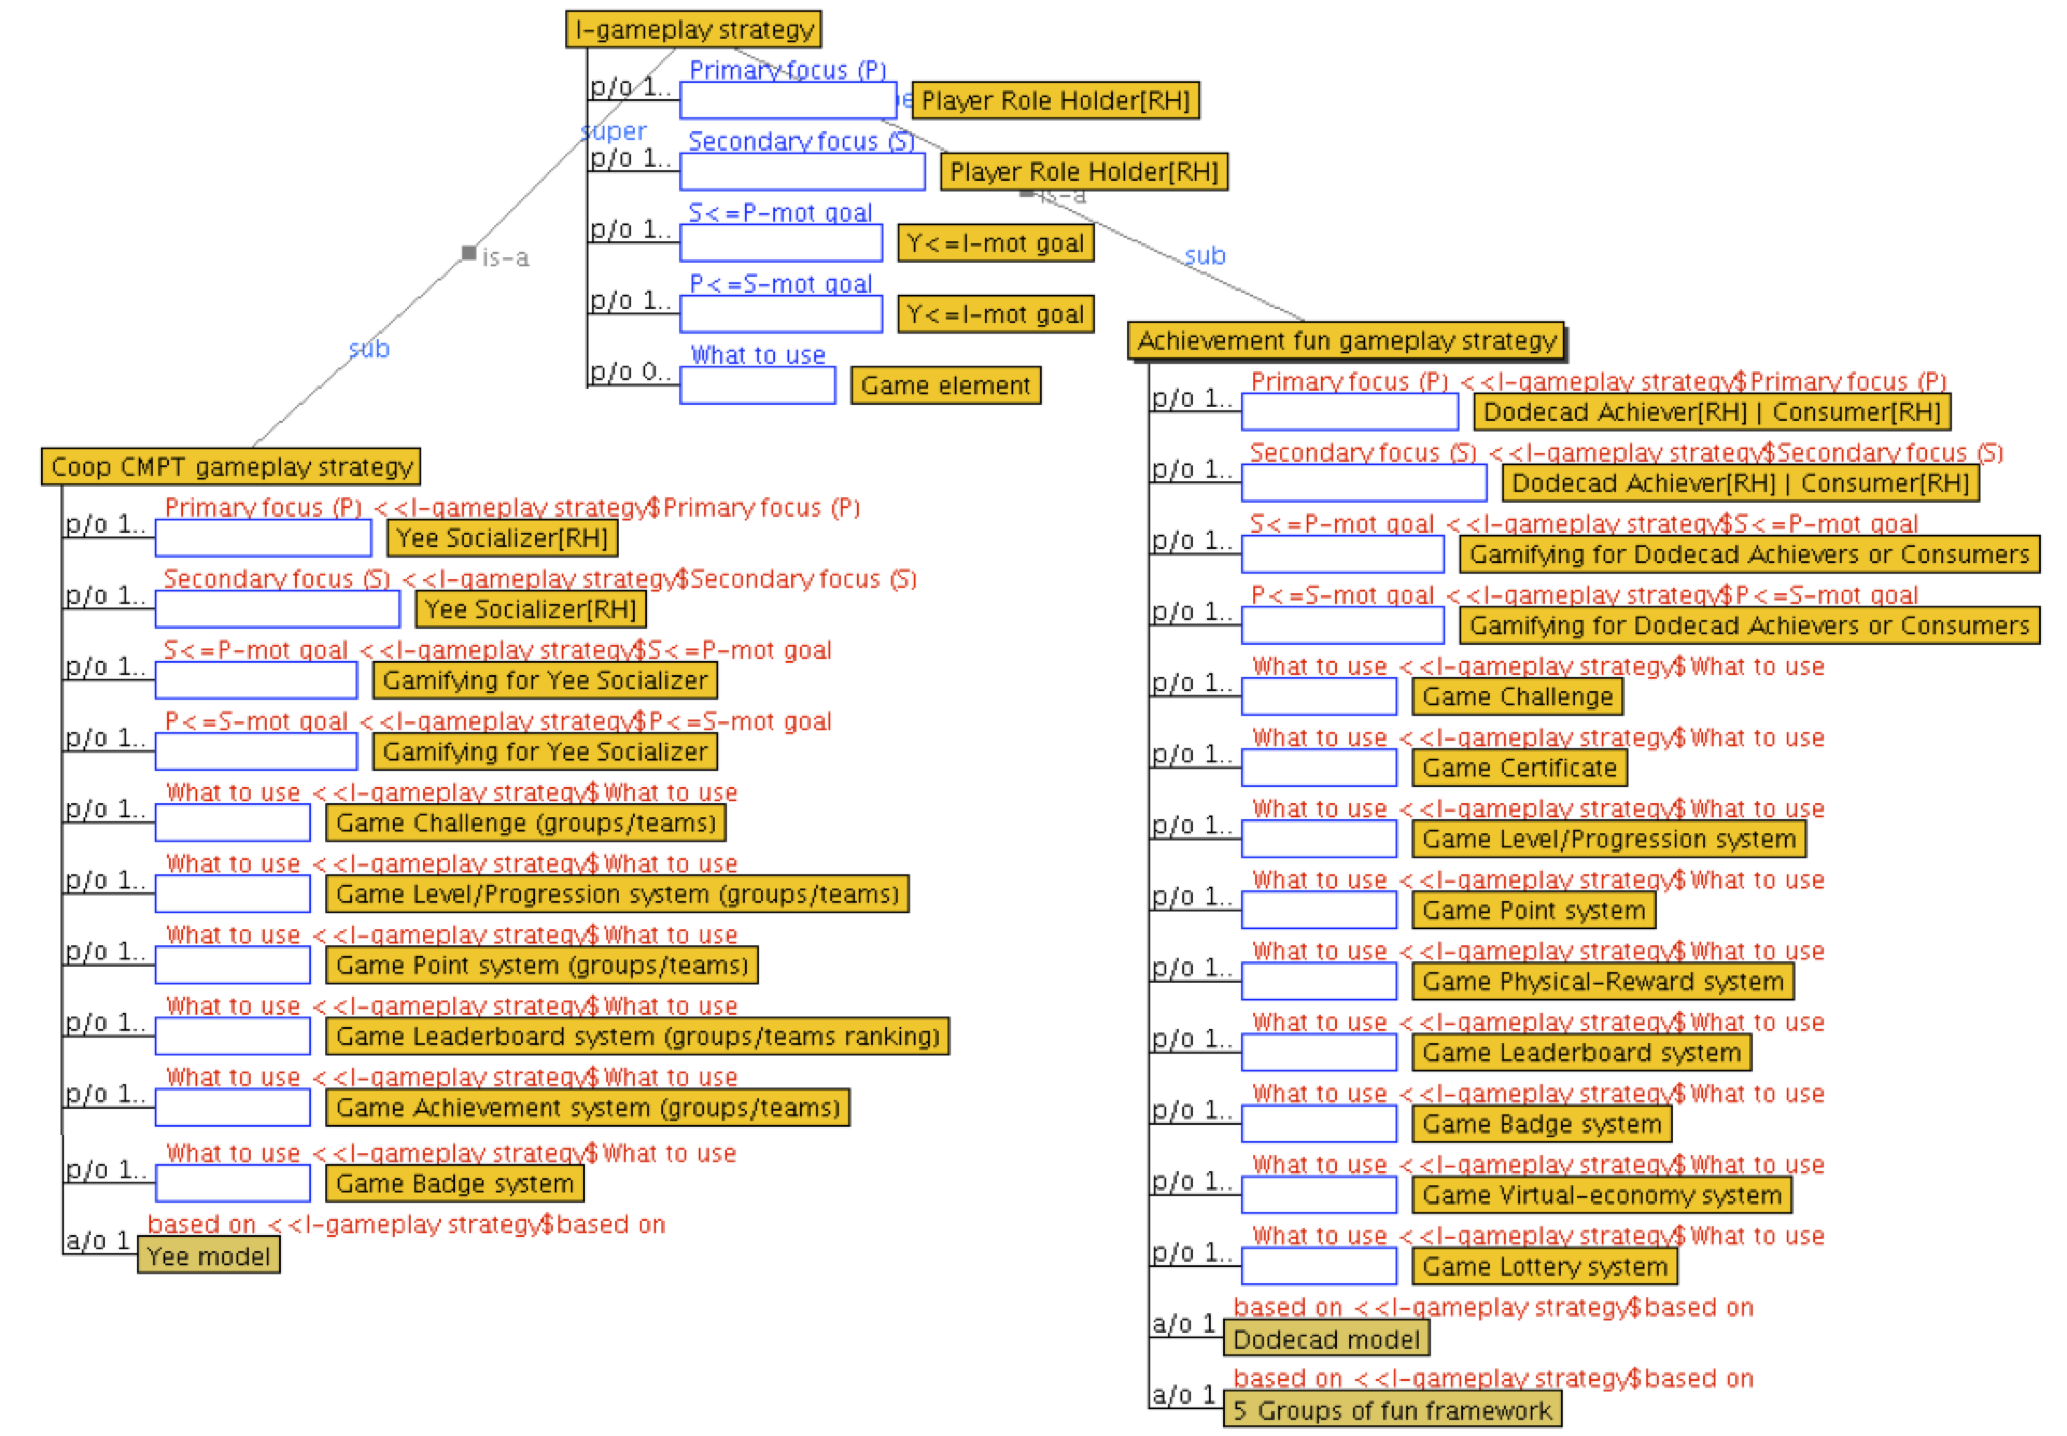
\includegraphics[width=1\textwidth]{images/chap-ontogacles1/ontological-structure-individual-gameplay-strategy.png} 
 \fautor
\end{figure}

The individual gameplay strategy depends of the player roles assigned for the participants of CL scenario, the motivational strategies employed to gamify the CL scenario, and the game elements introduced in the CL scenario. Thus, the ontological structure to represent an individual gameplay strategy is defined as a rational arrangement of these elements, where:

\begin{description}
\item [\textbf{Primary focus (P)}]
indicates the \emph{Player role holders} who are in the primary focus (P) of individual gameplay strategy. These player role holders are the participants who use the individual gameplay strategy (\emph{I-gameplay strategy}) to interact with the game elements indicated in the attribute \aspas{\emph{What to use}.}

\item [\textbf{Secondary focus (S)}]
indicates the \emph{Player role holders} who are in the secondary focus (S) of individual gameplay strategy. These player role holders are the participants who provide support for the player role holders in the primary focus (P) through the game elements indicated in the attribute \aspas{\emph{What to use}.} It means that the individual gameplay strategy (\emph{I-gameplay strategy}) is not necessary used by the participants in secondary focus (S) to interact with the game elements, but their interactions in the gamified CL scenario produce changes in the state of game elements indicated in the attribute \aspas{\emph{What to use}.}

\item[\textbf{S<=I-mot goal}]
indicates the motivational strategies employed in the gamified CL scenario to motivate the player role holders who are in the primary focus (P).

\item[\textbf{P<=S-mot goal}]
indicates the motivational strategies employed in the gamified CL scenario to motivate and engage the player role holders who are in the secondary focus (S).

\item[\textbf{What to use}]
indicates the game elements that are needed to carry out the individual gameplay strategy. Thus, the game elements defined in this attribute are the ones that are used to process the interactions of participants who are in the primary focus (P).
\end{description}

Currently, in the literature of gamification and game design, there is no one set of gameplay strategies established that could be directly formalized as individual gameplay strategies employing the ontological structure (\emph{I-gameplay strategy}) proposed here. Therefore, the author of this thesis has inferred some individual gameplay strategies employing the guidelines of gamification and game design models. \autoref{fig:ontological-structure-individual-gameplay-strategy} shows two examples of this formalization in which the guidelines described in the Yee's model \cite{Yee2006} have been used to formalize the cooperative competition gameplay strategy (\emph{Coop. CMPT gameplay strategy}) shown at the bottom-left of figure. According to this structure, a cooperative competition gameplay strategy is beneficial for participants who are holders of Yee's Socializer role, Primary focus (P), when the motivational strategy \aspas{\emph{Gamifying for Yee Socializer}} is applied in a CL scenario to motivate these group of participants to interact with other participants who are also holders of Yee's Socializer role, Secondary focus (S). In the attribute \aspas{\emph{What to use},} this structure also indicates that game challenges for groups/teams, game level/progression systems for groups/teams, game point system for groups/teams, game leaderboard system with groups/teams rankings, game achievement system for groups/teams, and game badge systems are necessary to implement the cooperative competition gameplay strategy.

\subsection{Gamified CL Scenario}
\label{subsec:gamified-cl-scenario}

A gamified CL scenario is a CL scenario in which the concepts previously presented in this section have been properly applied to gamify it. In this sense, to formally represent a gamified CL scenario in the ontology OntoGaCLeS, the ontological structures proposed in the CL ontology to represent a CL scenario (\autoref{fig:ontological-structure-cl-scenario}) has been extended by adding the representation of motivational strategies (\emph{Y<=I-mot goal}) and gameplay strategies (\emph{I-gameplay strategy}) at the same level that the learning strategies (\emph{Y<=I-goal}). The proper connection of these elements represents a \aspas{\emph{Gamified CL Scenario}} by the ontological structures shown in \autoref{fig:ontological-structure-gamified-cl-scenario}.

\begin{figure}[!htbp]
 \caption[Ontological structures to represent a gamified CL scenario]{Ontological structures to represent a \aspas{\emph{Gamified CL Scenario}}}
 \label{fig:ontological-structure-gamified-cl-scenario}
 \centering
 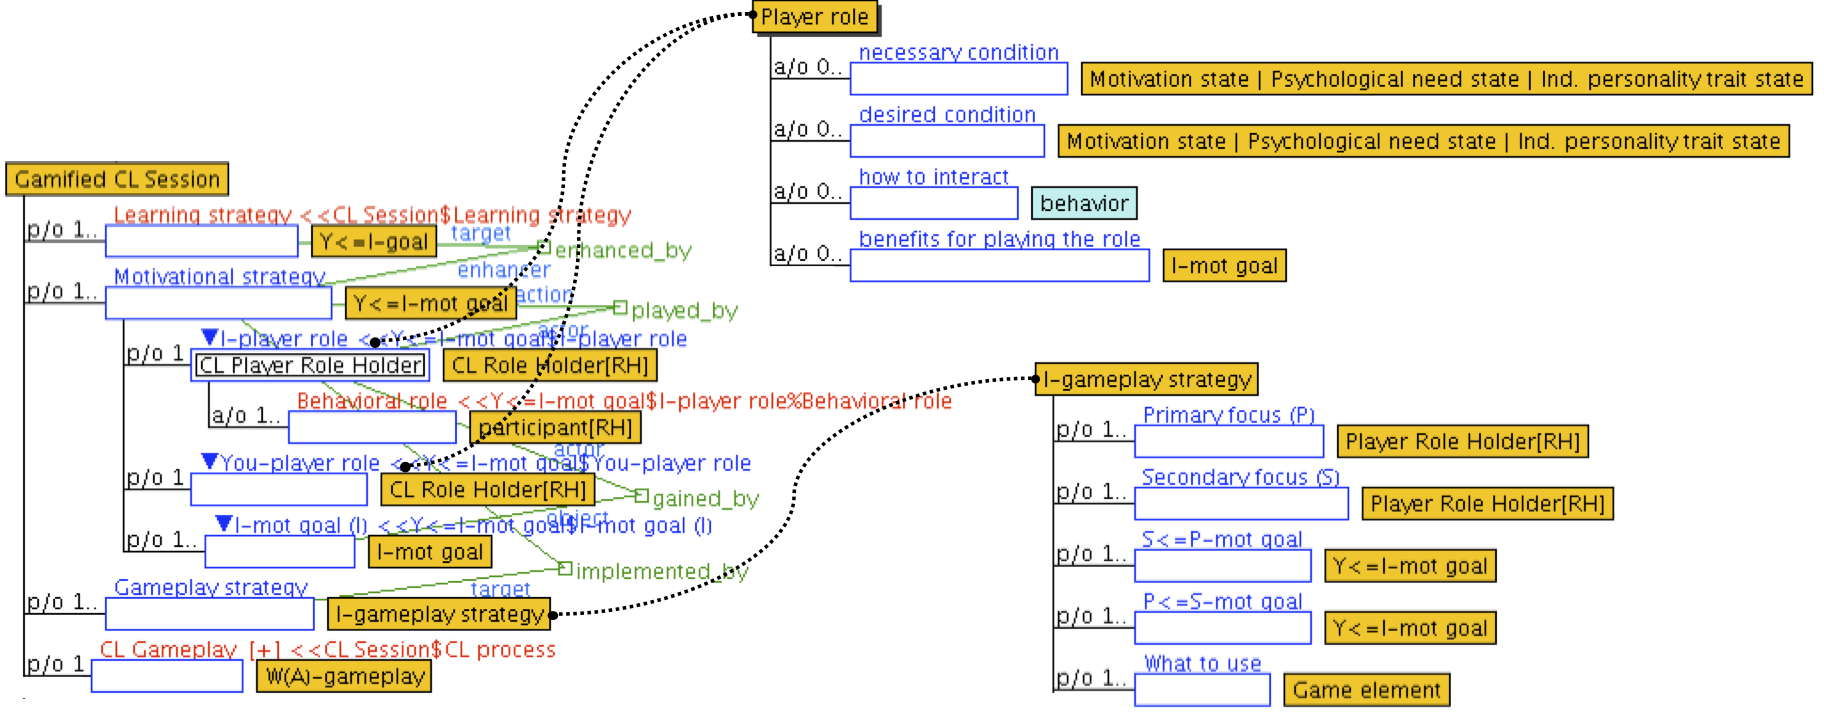
\includegraphics[width=1\textwidth]{images/chap-ontogacles1/ontological-structure-gamified-cl-scenario.png} 
 \fautor
\end{figure}

As was explained in previous subsections, the individual motivational strategy (\emph{Y<=I-mot goal}) describes the guidelines used to enhance the learning strategy employed by the participant in focus (\emph{I}), and the individual gameplay strategy (\emph{I-gameplay strategy}) describes the strategy used to implement the guidelines of individual motivational strategies. Based on these definitions, in the ontological structures to represent a gamified CL scenario (\autoref{fig:ontological-structure-gamified-cl-scenario}), the connection of these elements has been represented by the two relational-concepts: \aspas{\emph{enhanced\_by}} and \aspas{\emph{implemented\_by}.} The relational-concept \aspas{\emph{enhanced\_by}} indicates what individual motivational strategy (\emph{Y<=I-mot goal}) is used to enhance a learning strategy (\emph{Y<=I-goal}), and the relational-concept \aspas{\emph{implemented\_by}} indicates what individual gameplay strategy (\emph{I-gameplay strategy}) is used to implement the guidelines of an individual motivational strategy (\emph{Y<=I-mot goal}).

To illustrate the use of the ontological structures proposed in \autoref{fig:ontological-structure-gamified-cl-scenario}, a gamified CL scenario for participant who plays the Dodecad Socializers has been formalized as shown in \autoref{fig:ontological-structure-gamified-cl-scenario-dodecad-socializers}, where the learning strategies (\emph{Y<=I-goal}) of participants are \emph{enhanced by} the individual motivational strategy \aspas{\emph{Gamifying for Dodecad Socializer}.} According to this motivational strategy:

\begin{citacao}
\aspas{... Socializers are motivated by relatedness. They want to interact with others and create social connections ... Socializers are the ones who want to interact with others. They like to be connected to others. They are interested in parts of the system that help them do this. These are the ones will evangelize your internal social networks. Most motivated by the social connections aspects of relatedness ... Socializer and Networkers will wish to interact with people. Neither will be after anything from people directly. In the case of a networker, their reward comes from being connected; whereas the socialiser's reward is knowing you and interacting with you ...} \citeonline{Marczewski2015d}.
\end{citacao}

Based on these guidelines, the individual motivational strategy \aspas{\emph{Gamifying for Dodecad Socializer}} indicates that a participant who plays the Dodecad Socializer role (\emph{I-player role}) interacts with other socializer (\emph{You-player role}) acting as \emph{Helper} to achieve the \emph{Satisfaction of relatedness} (\emph{I-mot goal}). In this sense, the motivational strategy is \emph{implemented by} a \emph{Social fun gameplay strategy} (\emph{I-gameplay strategy}) in which, to support the communication and cooperation of participants, the game social-status and game social-connections were inferred as necessary game elements to carry out the social fun gameplay strategy. This inference pertains to the author of this thesis, and it consists in that participants who play the socializer role are interesting into help others by looking for social connections and status to satisfy his/her need of relatedness.

\begin{figure}[!htbp]
 \caption[Ontological structures to represent a gamified CL scenario for dodecad socializers]{Ontological structures to represent a \aspas{\emph{Gamified CL Scenario for Dodecad Socializers}}}
 \label{fig:ontological-structure-gamified-cl-scenario-dodecad-socializers}
 \centering
 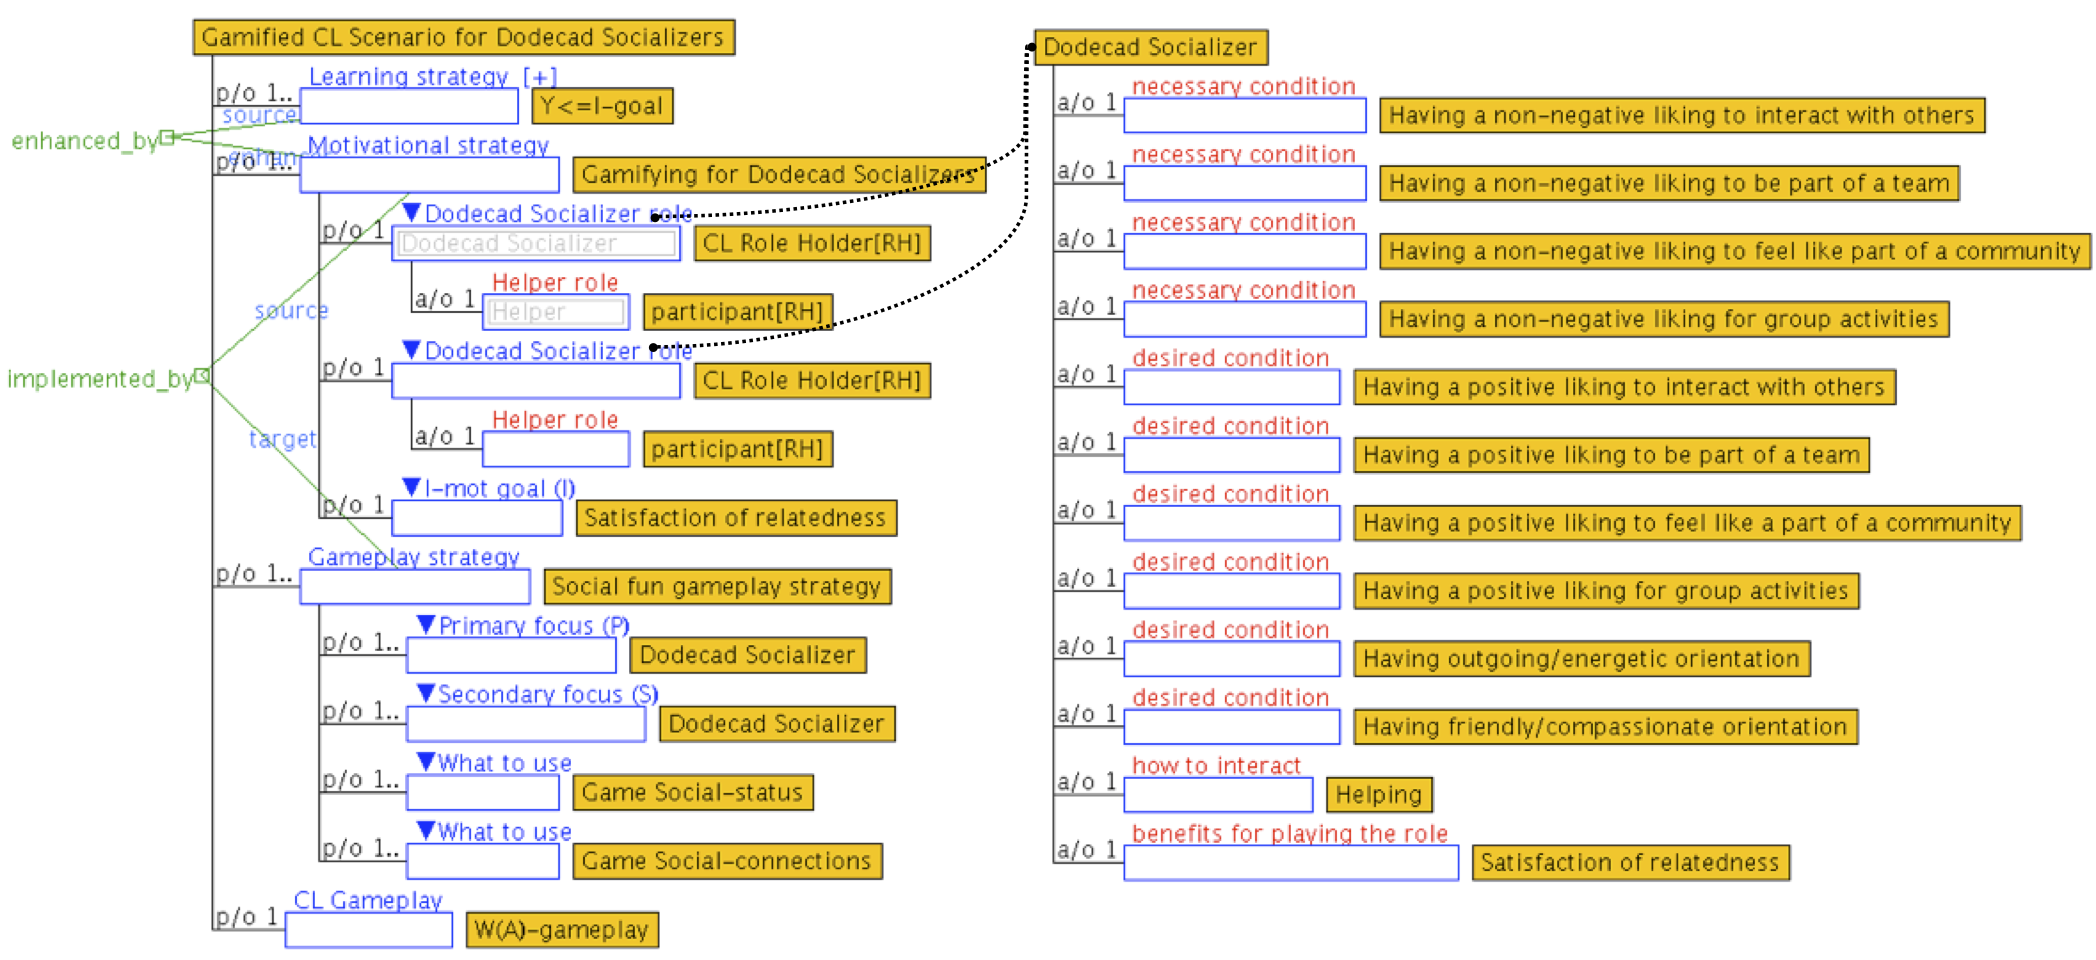
\includegraphics[width=1\textwidth]{images/chap-ontogacles1/ontological-structure-gamified-cl-scenario-dodecad-socializers.png} 
 \fautor
\end{figure}

%%%%%%%%%%%%%%%%%%%%%%%%%%%%%%%%%%%%%%%%%%%%%%%%%%%%

\section[Formalizing an Ontological Model to Personalize the Gamification in CL Scenarios]{Formalizing an Ontological Model to Personalize the Gamification in Collaborative Learning Scenarios}
\label{sec:formalizing-ontological-model}

Through the use of ontological structures presented in the previous section, the author of this thesis expects to facilitate the systematic formalization of gamified CL scenarios based on concepts extracted from player types models and need-based theories of motivation. With this formalization, it is possible to built ontological models to personalize the gamification in CL scenario. These models consist in a set of gamified CL scenarios formally represented as the ontological structures proposed in \autoref{fig:ontological-structure-gamified-cl-scenario}. The building of these structures to define an ontological model comprises the following steps: (1) to identify the player roles that can be assigned for the participants of CL scenario when they are playing a CL role, (2) to identify the restriction and elements of motivational strategies for each pair of identified player roles, and (3) to define individual gameplay strategies for the identified pairs of player roles.

In this section, following these steps, the building of an ontological model to personalize the gamification in CL scenario is detailed in this section. This model has been built to gamify CL scenarios based on the Peer-tutoring theory \cite{Endlsey1980} in which the Dodecad player type model \cite{Marczewski2017,Marczewski2015b} have been used as source of information to formalize this model. 

\subsubsection*{Step (1): Identifying Player Roles for CL Scenarios}  

The identification of player roles to gamify a CL scenario is carried out by analyzing the expected behaviors to be externalized for these roles and the CL roles. Possible counterproductive behaviors indicate what player roles cannot be assigned to a participant when he/she plays the CL role. \autoref{tab:player-roles-in-peer-tutoring-cl-scenarios} shows the result of this step (1) for the CL roles of \aspas{\emph{Peer-Tutor}} and \aspas{\emph{Peer-Tutee}} defined in CL Scenarios based on the Peer-tutoring theory. Counterproductive behaviors of player roles are avoided to not interfere with the expected behaviors of CL roles. Thus, for example, participants who are playing the CL roles of Peer-tutor and Peer-tutee cannot play the \emph{Griefer roles} because they want to negatively affect other users.

\setlongtables{\small
\begin{longtable}{lcc}
\caption[Dodecad player roles that can be assigned for participants of a Peer-tutoring scenario]{Dodecad player roles that can be assigned for participants of a Peer-tutoring scenario}
\tabularnewline
\hline\hline
\multicolumn{1}{l}{}&
\multicolumn{1}{c}{\textbf{Peer-Tutor}}&
\multicolumn{1}{c}{\textbf{Peer-Tutee}}\tabularnewline
\multicolumn{1}{l}{}&
\multicolumn{1}{c}{\footnotesize(explaining)}&
\multicolumn{1}{c}{\footnotesize(passive learning)}\tabularnewline
\hline
\endfirsthead\caption[]{\em (continued)} \tabularnewline
\hline
\multicolumn{1}{l}{}&
\multicolumn{1}{c}{\textbf{Peer-Tutor}}&
\multicolumn{1}{c}{\textbf{Peer-Tutee}}\tabularnewline
\multicolumn{1}{l}{}&
\multicolumn{1}{c}{\footnotesize(explaining)}&
\multicolumn{1}{c}{\footnotesize(passive learning)}\tabularnewline
\hline
\endhead
\hline
\endfoot
\label{tab:player-roles-in-peer-tutoring-cl-scenarios}

\textbf{Achiever}&\multirow{2}{*}{Yes}&\multirow{2}{*}{Yes}\tabularnewline
{\footnotesize(accomplishing, comparing)}& & \tabularnewline
\hline

\textbf{Free-Spirit}&No&No\tabularnewline
{\footnotesize(creating, exploring)}&{\footnotesize(don't want to be restricted)}&{\footnotesize(don't want to be restricted)}\tabularnewline
\hline

\textbf{Socializer}&\multirow{2}{*}{Yes}&\multirow{2}{*}{Yes}\tabularnewline
{\footnotesize(helping)}& & \tabularnewline
\hline

\textbf{Philanthropist}&\multirow{2}{*}{Yes}&\multirow{2}{*}{Yes}\tabularnewline
{\footnotesize(giving, helping, sharing)}& & \tabularnewline
\hline

\textbf{Consumer}&\multirow{2}{*}{Yes}&\multirow{2}{*}{Yes}\tabularnewline
{\footnotesize(accomplishing, comparing)}& & \tabularnewline
\hline

\textbf{Exploiter}&No&No\tabularnewline
{\footnotesize(creating, exploring)}&{\footnotesize(don't want to be restricted)}&{\footnotesize(don't want to be restricted)} \tabularnewline
\hline

\textbf{Networker}&\multirow{2}{*}{Yes}&\multirow{2}{*}{Yes}\tabularnewline
{\footnotesize(helping)}& & \tabularnewline
\hline

\textbf{Self-Seeker}&\multirow{2}{*}{Yes}&\multirow{2}{*}{Yes}\tabularnewline
{\footnotesize(giving, helping, sharing)}& & \tabularnewline
\hline

\textbf{Destroyer}&No&No \tabularnewline
{\footnotesize(hacking)}&{\footnotesize(hacking to ruin experience of others)}&{\footnotesize(hacking to ruin experience of others)}\tabularnewline
\hline

\textbf{Improver}&No&No\tabularnewline
{\footnotesize(hacking, exploring, fixing)}&{\footnotesize(hacking to change the system)}&{\footnotesize(hacking to change the system)}\tabularnewline
\hline

\textbf{Influencer}&No&No \tabularnewline
{\footnotesize(commenting)}&{\footnotesize(requiring changes in the system)}&{\footnotesize(requiring changes in the system)} \tabularnewline
\hline

\textbf{Griefer}&No&No\tabularnewline
{\footnotesize(troublemaking, defying)}&{\footnotesize(negatively affect to others)}&{\footnotesize(negatively affect to others)}\tabularnewline

\hline
\end{longtable}
}

\subsubsection*{Step (2): Identifying Restrictions and Elements of Motivational Strategies}

To identify the restrictions and elements of individual motivational strategies (\emph{Y<=I-mot goal}), guidelines for the pairs of player roles identified in the step (1) are crossed. These guidelines are extracted from the player type models for the building of ontological models to personalize the gamification in CL scenarios. When these guidelines related to a pair of player roles are crossed, counterproductive behaviors are avoided to not interfere with the expected benefits that can be achieved by the participants playing these roles and performing these behaviors. The expected benefits are expressed as individual motivational goals (\emph{I-mot goals}) based on interpretation of these benefits using need-based theories of motivation. 

\autoref{tab:individual-motivational-strategies-in-peer-tutoring-cl-scenarios} shows the result obtained in this step for the definition of individual motivational strategies in the ontological model to personalize the gamification in Peer-tutoring CL scenarios. The rows indicate the player roles (\emph{I-Player role}) for the participant in focus (\emph{I}), and the columns indicate the player roles (\emph{You-Player role}) for the participant (\emph{You}) who interacts with the participant in focus (\emph{I}). The individual gameplay strategies and their elements are indicated in the crossed cells. These strategies were defined from common guidelines for each pair of player roles. Thus, an individual gameplay strategy has been formalized in the ontological model when there are common expected behaviors indicated in the guidelines of player roles \aspas{\emph{I-Player role}} and \aspas{\emph{You-Player role}.}
 

\setlongtables\begin{landscape}{\small
\begin{longtable}{|l|c|c|c|c|c|c|}
\caption[Individual motivational strategies identified for the building of an ontological model to personalize the gamification in Peer-tutoring scenarios]{Individual motivational strategies identified for the building of an ontological model to personalize the gamification in Peer-tutoring scenarios}
\tabularnewline
\hline\hline
\multicolumn{1}{|l|}{}&
\multicolumn{1}{c|}{\textbf{Achiever}}&
\multicolumn{1}{c|}{\textbf{Socializer}}&
\multicolumn{1}{c|}{\textbf{Philanthropist}}&
\multicolumn{1}{c|}{\textbf{Consumer}}&
\multicolumn{1}{c|}{\textbf{Networker}}&
\multicolumn{1}{c|}{\textbf{Self-seeker}}\tabularnewline
\multicolumn{1}{|l|}{}&
\multicolumn{1}{c|}{\tiny{(\emph{accomplishing, comparing})}}&
\multicolumn{1}{c|}{\tiny{(\emph{helping})}}&
\multicolumn{1}{c|}{\tiny{(\emph{giving, helping, sharing})}}&
\multicolumn{1}{c|}{\tiny{(\emph{accomplishing, comparing})}}&
\multicolumn{1}{c|}{\tiny{(\emph{helping})}}&
\multicolumn{1}{c|}{\tiny{(\emph{giving, helping, sharing})}}\tabularnewline
\hline
\endfirsthead\caption[]{\em (continued)} \tabularnewline
\hline
\multicolumn{1}{|l|}{}&
\multicolumn{1}{c|}{\textbf{Achiever}}&
\multicolumn{1}{c|}{\textbf{Socializer}}&
\multicolumn{1}{c|}{\textbf{Philanthropist}}&
\multicolumn{1}{c|}{\textbf{Consumer}}&
\multicolumn{1}{c|}{\textbf{Networker}}&
\multicolumn{1}{c|}{\textbf{Self-seeker}}\tabularnewline
\multicolumn{1}{|l|}{}&
\multicolumn{1}{c|}{\tiny{(\emph{accomplishing, comparing})}}&
\multicolumn{1}{c|}{\tiny{(\emph{helping})}}&
\multicolumn{1}{c|}{\tiny{(\emph{giving, helping, sharing})}}&
\multicolumn{1}{c|}{\tiny{(\emph{accomplishing, comparing})}}&
\multicolumn{1}{c|}{\tiny{(\emph{helping})}}&
\multicolumn{1}{c|}{\tiny{(\emph{giving, helping, sharing})}}\tabularnewline
\hline
\endhead
\hline
\endfoot
\label{tab:individual-motivational-strategies-in-peer-tutoring-cl-scenarios}
&
\multicolumn{1}{p{3cm}|}{\tiny\emph{Gamifying for Dodecad Achievers}}& & &
\multicolumn{1}{p{3cm}|}{\tiny\emph{Gamifying for Dodecad Achievers and Consumer}}& &  \tabularnewline
{\textbf{Achiever}}&
\multicolumn{1}{p{3cm}|}{\tiny{$\bullet$ Satisfaction of mastery}}& & &
\multicolumn{1}{p{3cm}|}{\tiny{$\bullet$ Satisfaction of mastery}}& & \tabularnewline
{\tiny(\emph{accomplishing, comparing})}&
\multicolumn{1}{p{3cm}|}{}& & &
\multicolumn{1}{p{3cm}|}{\tiny{$\bullet$ Internalization from extrinsic to intrinsic motivation}}& & \tabularnewline
\hline

& &
\multicolumn{1}{p{3cm}|}{\tiny\emph{Gamifying for Dodecad Socializers}}& & &
\multicolumn{1}{p{3cm}|}{\tiny\emph{Gamifying for Dodecad Socializer and Networker}}& \tabularnewline
{\textbf{Socializer}}& &
\multicolumn{1}{p{3cm}|}{\tiny{$\bullet$ Satisfaction of relatedness}}& & &
\multicolumn{1}{p{3cm}|}{\tiny{$\bullet$ Satisfaction of relatedness}}& \tabularnewline
{\tiny(\emph{helping})}& & 
\multicolumn{1}{p{3cm}|}{}& & &
\multicolumn{1}{p{3cm}|}{\tiny{$\bullet$ Internalization from extrinsic to intrinsic motivation}}& \tabularnewline
\hline

\textbf{Philanthropist}& & &
\multicolumn{1}{p{3cm}|}{\tiny\emph{Gamifying for Philanthropists}}& & &
\multicolumn{1}{p{3cm}|}{\tiny\emph{Gamifying for Philanthropist and Self-seeker}}\tabularnewline
{\tiny(\emph{giving, helping, sharing})}& & &
\multicolumn{1}{p{3cm}|}{\tiny{$\bullet$ Satisfaction of purpose}}& & &
\multicolumn{1}{p{3cm}|}{\tiny{$\bullet$ Satisfaction of purpose}}\tabularnewline
& & &
\multicolumn{1}{p{3cm}|}{}& & &
\multicolumn{1}{p{3cm}|}{\tiny{$\bullet$ Internalization from extrinsic to intrinsic motivation}}\tabularnewline
\hline

&
\multicolumn{1}{p{3cm}|}{\tiny\emph{Gamifying for Consumer and Dodecad Achiever}}& & &
\multicolumn{1}{p{3cm}|}{\tiny\emph{Gamifying for Consumers}}& &  \tabularnewline
{\textbf{Consumer}}&
\multicolumn{1}{p{3cm}|}{\tiny{$\bullet$ Satisfaction of mastery}}& & &
\multicolumn{1}{p{3cm}|}{\tiny{$\bullet$ Satisfaction of mastery}}& & \tabularnewline
{\tiny(\emph{accomplishing, comparing})}&
\multicolumn{1}{p{3cm}|}{\tiny{$\bullet$ Internalization from extrinsic to intrinsic motivation}}& & &
\multicolumn{1}{p{3cm}|}{}& & \tabularnewline \newpage
\hline

& &
\multicolumn{1}{p{3cm}|}{\tiny\emph{Gamifying for Networker and Dodecad Socializer}}& & &
\multicolumn{1}{p{3cm}|}{\tiny\emph{Gamifying for Networkers}}&  \tabularnewline
{\textbf{Networker}}& &
\multicolumn{1}{p{3cm}|}{\tiny{$\bullet$ Satisfaction of relatedness}}& & &
\multicolumn{1}{p{3cm}|}{\tiny{$\bullet$ Satisfaction of relatedness}}& \tabularnewline
{\tiny(\emph{helping})}& & 
\multicolumn{1}{p{3cm}|}{\tiny{$\bullet$ Internalization from extrinsic to intrinsic motivation}}& & &
\multicolumn{1}{p{3cm}|}{}& \tabularnewline
\hline

& & &
\multicolumn{1}{p{3cm}|}{\tiny\emph{Gamifying for Self-seeker and Philanthropist}}& & &
\multicolumn{1}{p{3cm}|}{\tiny\emph{Gamifying for Philanthropists}}\tabularnewline
{\textbf{Self-seeker}}& & &
\multicolumn{1}{p{3cm}|}{\tiny{$\bullet$ Satisfaction of purpose}}& & &
\multicolumn{1}{p{3cm}|}{\tiny{$\bullet$ Satisfaction of purpose}}\tabularnewline
{\tiny(\emph{giving, helping, sharing})}& & &
\multicolumn{1}{p{3cm}|}{\tiny{$\bullet$ Internalization from extrinsic to intrinsic motivation}}& & &
\multicolumn{1}{p{3cm}|}{}\tabularnewline
\hline
\end{longtable}
}\end{landscape}

To illustrate the identification of restrictions and elements in the individual motivational strategy (\emph{Y<=I-mot goal}), let us see the \aspas{\emph{Gamifying for Dodecad Achiever and Conqueror}} indicated in \autoref{tab:individual-motivational-strategies-in-peer-tutoring-cl-scenarios}, this strategy was identified from the guidelines of Dodecad model in which the behaviors of \emph{accomplishing} and \emph{comparing} are indicated as adequate to motivate achievers and consumers. In this case, the expected benefits to accomplish a goal, and then, compare it against the accomplishments of others is enjoyable for achievers. This benefit is represented as the individual motivational goal \aspas{\emph{Satisfaction of mastery}} (\emph{I-mot goal}) based on the Dan Pink motivation theory \cite{Pink2011}. According to this theory, mastery is a inherit human need that love to get better at stuff enjoying satisfaction from personal achievement and progress.
 
\subsubsection*{Step (3): Defining Individual Gameplay Strategies}

Individual gameplay strategies (\emph{I-gameplay strategy}) are inferred from the individual motivational strategies (\emph{Y<=I-mot goal}) identified in the step (2). Game elements are defined to support the behaviors indicated in the guidelines of individual motivational strategies, and so obtain the expected benefits indicated as individual motivational goal. \autoref{tab:individual-gameplay-strategies-peer-tutoring-cl-scenarios} shows the results of this step for the ontological model to personalize the gamification in Peer-tutoring scenarios.

\setlongtables{\small
\begin{longtable}{l|l|l}
\caption[Individual gameplay strategies to gamify Peer-tutoring scenarios]{Individual gameplay strategies to gamify Peer-tutoring scenarios}
\tabularnewline
\hline\hline
\multicolumn{1}{p{4.75cm}}{\centering\textbf{Achievement fun}}&
\multicolumn{1}{|p{4.75cm}|}{\centering\textbf{Social fun}}&
\multicolumn{1}{p{4.75cm}}{\centering\textbf{Facilitated-personal fun}}\tabularnewline
\hline
\endfirsthead\caption[]{\em (continued)} \tabularnewline
\hline
\multicolumn{1}{p{4.75cm}}{\centering\textbf{Achievement fun}}&
\multicolumn{1}{|p{4.75cm}|}{\centering\textbf{Social fun}}&
\multicolumn{1}{p{4.75cm}}{\centering\textbf{Facilitated-personal fun}}\tabularnewline
\hline
\endhead
\hline
\endfoot
\label{tab:individual-gameplay-strategies-peer-tutoring-cl-scenarios}

Primary focus (P):&
Primary focus (P):&
Primary focus (P):\tabularnewline

{\scriptsize$\bullet$ Gamifying for Dodecad Achiever}&
{\scriptsize$\bullet$ Gamifying for Dodecad Socializer}&
{\scriptsize$\bullet$ Gamifying for Philanthropists}\tabularnewline

{\scriptsize$\bullet$ Gamifying for Consumer}&
{\scriptsize$\bullet$ Gamifying for Networker}&
{\scriptsize$\bullet$ Gamifying for Self-seekers}\tabularnewline


Secondary focus (S):&
Secondary focus (S):&
Secondary focus (S):\tabularnewline

{\scriptsize$\bullet$ Gamifying for Consumer}&
{\scriptsize$\bullet$ Gamifying for Networker}&
{\scriptsize$\bullet$ Gamifying for Self-seekers}\tabularnewline

{\scriptsize$\bullet$ Gamifying for Dodecad Achiever}&
{\scriptsize$\bullet$ Gamifying for Dodecad Socializer}&
{\scriptsize$\bullet$ Gamifying for Philanthropists}\tabularnewline
\hline

What to use:&
What to use:&
What to use:\tabularnewline

$\bullet$ Challenges&
$\bullet$ Social-status&
$\bullet$ Meaning/purpose\tabularnewline

$\bullet$ Certificates&
$\bullet$ Point system&
$\bullet$ Access system\tabularnewline

$\bullet$ Levels/progression system&
(\emph{social status})&
$\bullet$ Collect/trade system\tabularnewline

$\bullet$ Point system&
$\bullet$ Physical-reward system&
$\bullet$ Gifting/sharing system\tabularnewline

(\emph{levels/progression})&
(\emph{social status})&
$\bullet$ Point system\tabularnewline

$\bullet$ Physical-reward system&
$\bullet$ Leaderboard system&
(\emph{meaning/purpose})\tabularnewline

(\emph{certificates})&
(\emph{social status})&
$\bullet$ Physical-reward system\tabularnewline

$\bullet$ Leaderboard system&
$\bullet$ Badge system&
(\emph{meaning/purpose})\tabularnewline

(\emph{levels/progression})&
(\emph{social status})&
$\bullet$ Leaderboard system\tabularnewline

$\bullet$ Badge system&
$\bullet$ Virtual-economy system&
(\emph{meaning/purpose})\tabularnewline

(\emph{level/progression})&
$\bullet$ Lottery system&
$\bullet$ Badge system\tabularnewline

$\bullet$ Virtual-economy system&
&
(\emph{meaning/purpose})\tabularnewline

$\bullet$ Lottery system&
&
$\bullet$ Virtual economy system\tabularnewline

&
&
$\bullet$ Lottery system\tabularnewline

\hline
\end{longtable}
}

The individual gameplay strategies indicated in the \autoref{tab:individual-gameplay-strategies-peer-tutoring-cl-scenarios} are:

\begin{itemize}
\item \emph{Achievement fun gameplay strategy}:
is an individual motivational strategy in which the system recognizes achievements through game challenges, certificates and level/progression. To satisfy the mastery need, the system must try to produce in the participants the feel that they are achieving something by performing the interactions indicated by the Peer-tutoring scripts. Thus, the system would use a point system to indicate the levels/progression in the CSCL script, and when the CL scenario is completed as a game challenge, a certificate would be given by a physical-reward system. The leaderboard system would indicate the level/progression of the script. Badges would be obtained by the participants at the end of CL scenario according to the level/progression in the script. Finally, virtual-economy and lottery systems would establish the relation between the levels/progression of the script and the points, ranking in the leaderboard and badges.

\item \emph{Social fun gameplay strategy}:
is an individual motivational strategy in which social status is used to support the feeling of relatedness. In this sense, the system should provide some form of social network/group to indicate and/or create group/collective game elements. Thus, the system would use a points system with a social status system to indicate points gathered by the participant as group. When the CL scenario is completed, the system would give a physical reward for the groups. A leaderboard would provide rankings by groups to indicate the social status of groups. Badges for groups with a social status would be given by the system to groups when the CL scenario is completed. Finally, virtual-economy and lottery systems would establish the relation between the social status of groups in CL scenarios, and the points, physical-rewards, leaderboards, and badges.

\item \emph{Facilitated-personal fun gameplay strategy}:
is an individual motivational strategy in which the excitement from changing the system satisfy the need of purpose. This satisfaction comes from collection and trading valuable things. So when participants help to others, game elements are collected to be converted into something that has a meaningful value. Thus, meaning/purpose should be given to game elements such as points, physical-rewards, leaderboards, and badges, so that the system provides a collect/trade system to change these element for gifting and/or sharable elements (such as elements to customize the avatars, elements to change part of the system).
\end{itemize}

Employing the information of \autoref{tab:individual-gameplay-strategies-peer-tutoring-cl-scenarios}, twelve ontological structures to represent gamified Peer-tutoring scenarios have been formalized in the ontology OntoGaCLeS to define the model to personalize the gamification in Peer-tutoring scenarios based on the Dodecad model \cite{Marczewski2015b}. These structures in the ontological model are: \emph{Gamified Peer Tutoring Scenario for Achievers}, \emph{Gamified Peer Tutoring Scenario for Achiever/Consumer}, \emph{Gamified Peer Tutoring Scenario for Consumer/Achiever}, \emph{Gamified Peer Tutoring Scenario for Consumers}, \emph{Gamified Peer Tutoring Scenario for Socializers}, \emph{Gamified Peer Tutoring Scenario for Socializer/Networker}, \emph{Gamified Peer Tutoring Scenario for Networker/Socializer}, \emph{Gamified Peer Tutoring Scenario for Networkers}, \emph{Gamified Peer Tutoring Scenario for Philanthropists}, \emph{Gamified Peer Tutoring Scenario for Philanthropist/Self-seeker}, \emph{Gamified Peer Tutoring Scenario for Self-seeker/Philanthropist}, and \emph{Gamified Peer Tutoring Scenario for Self-seekers}. 


\begin{figure}[!htbp]
 \caption[Ontological structures to represent a gamified CL scenario for dodecad socializers]{Ontological structure to represent \aspas{\emph{Gamified Peer Tutoring Scenario for Achiever/Consumer}}}
 \label{fig:ontological-structure-gamified-peer-tutoring-scenario-achiever-consumer}
 \centering
  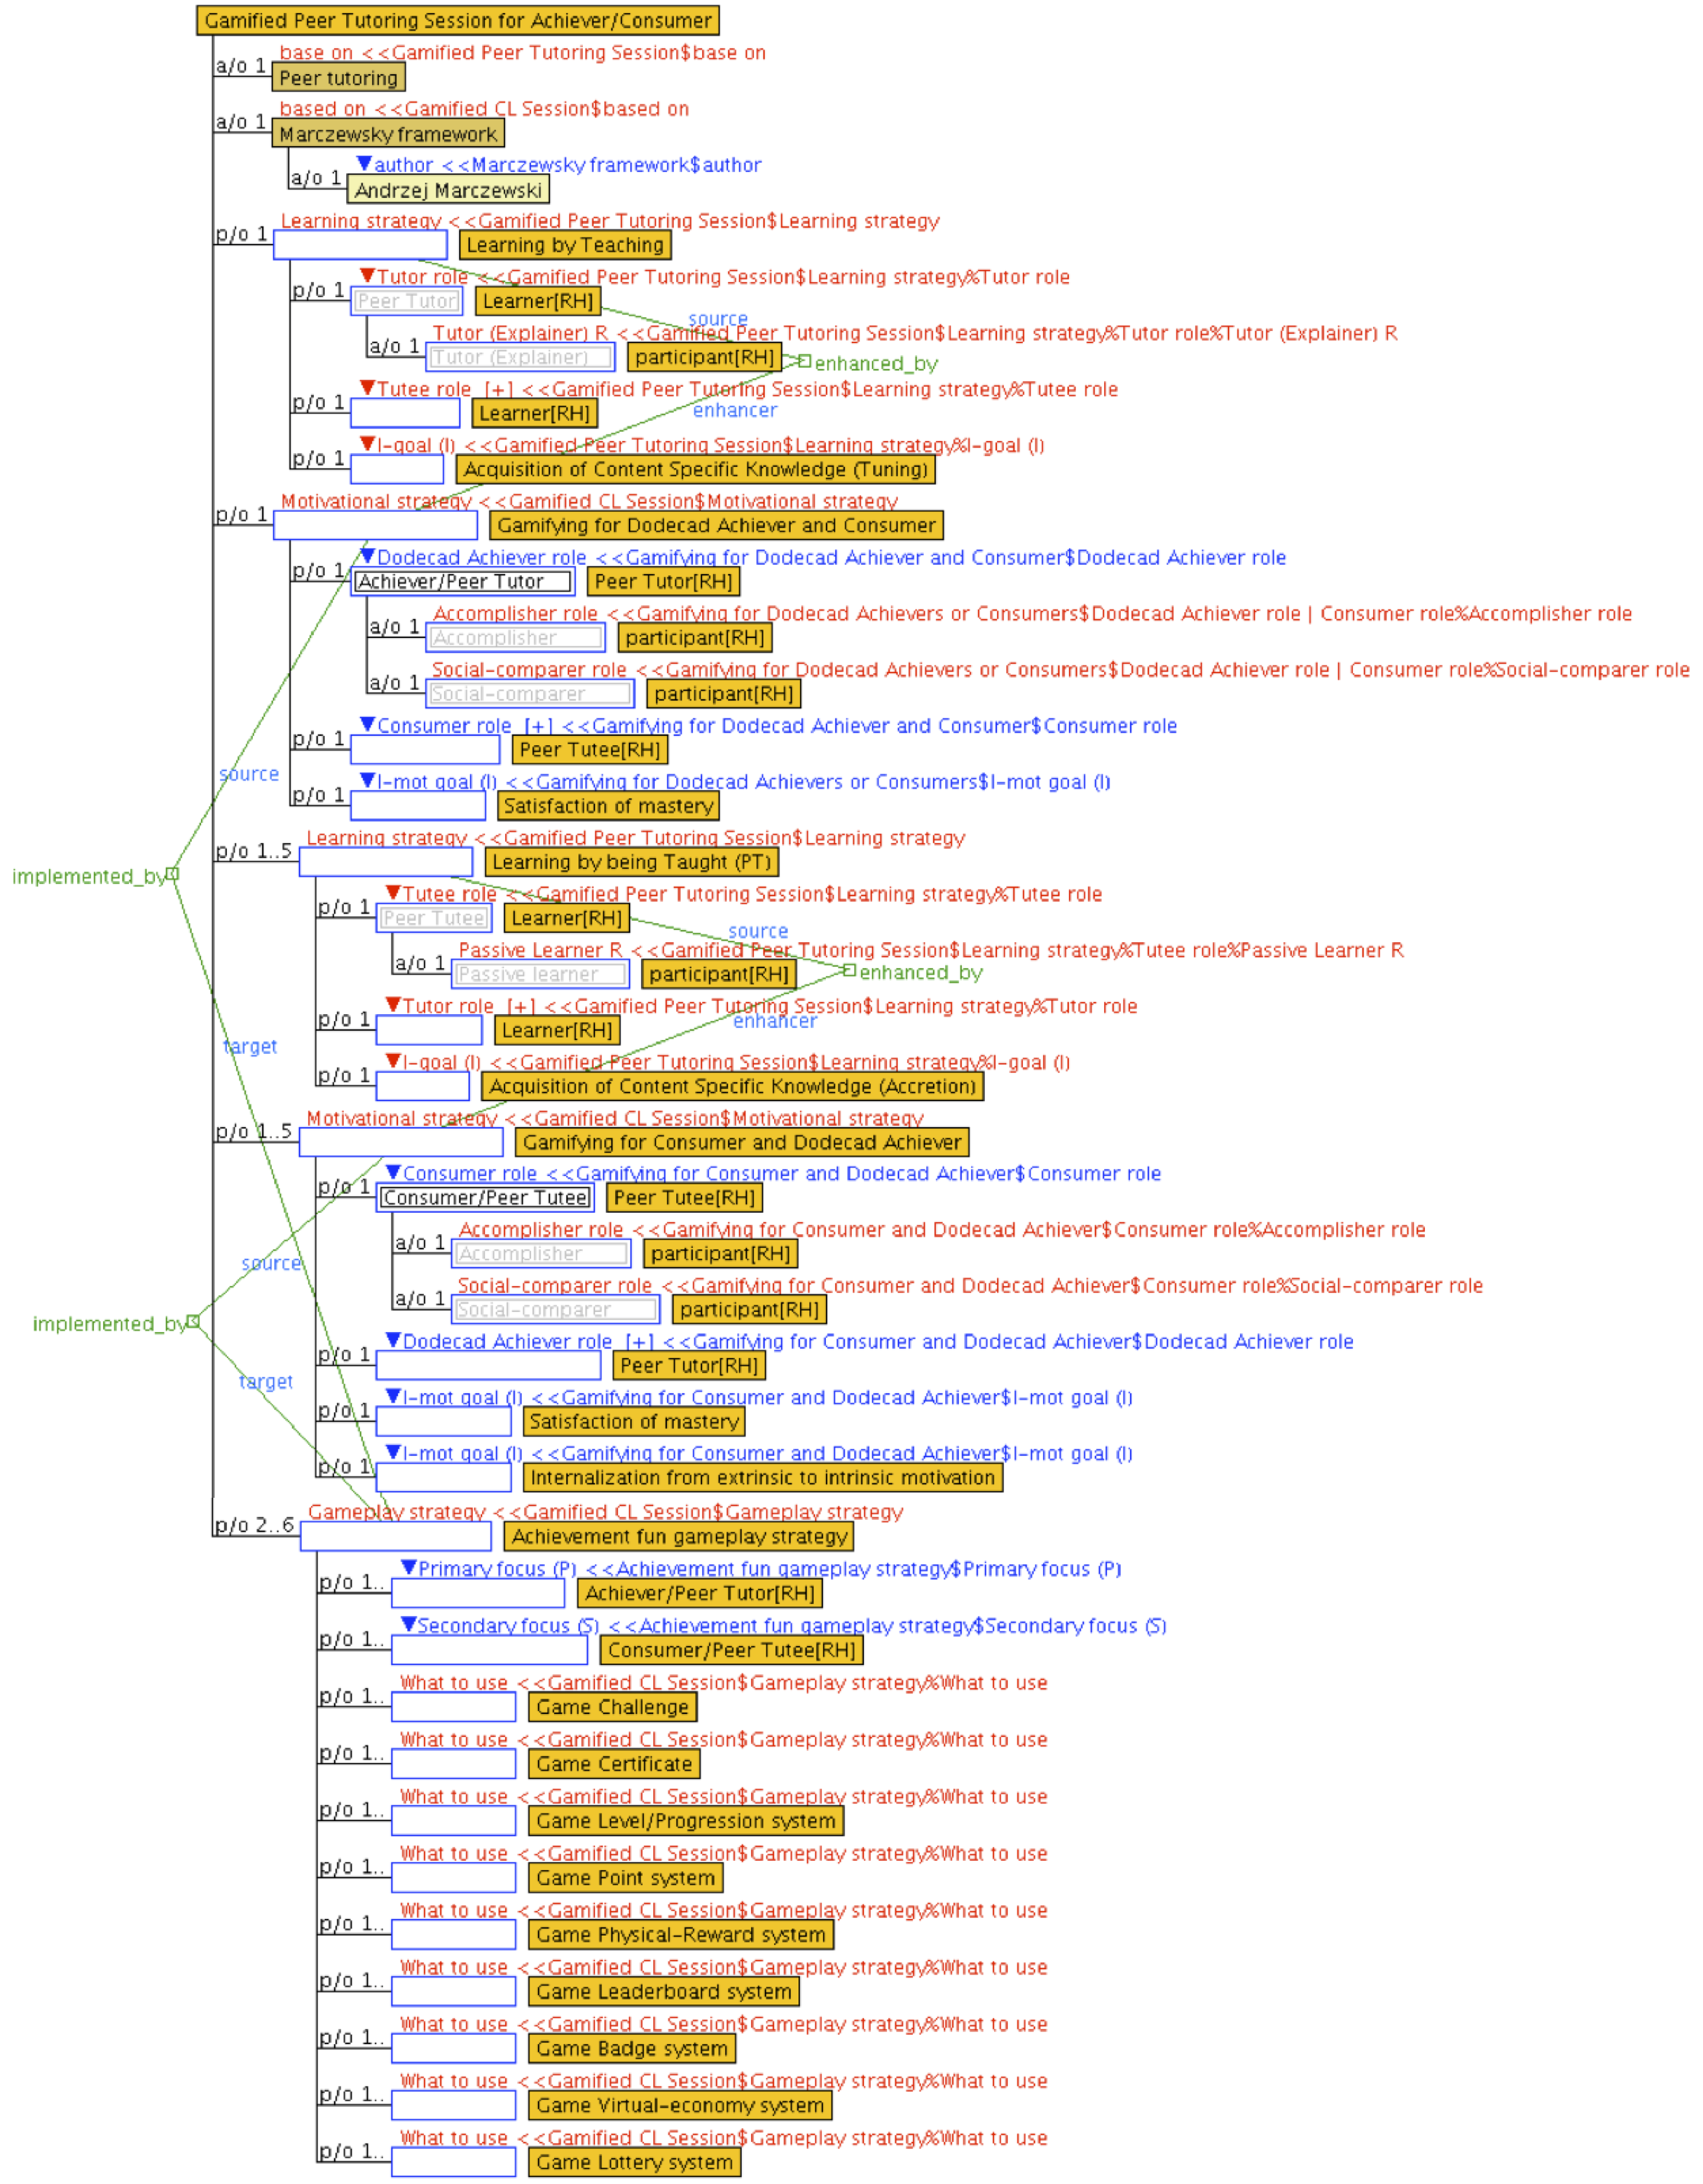
\includegraphics[width=1\textwidth]{images/chap-ontogacles1/ontological-structure-gamified-peer-tutoring-scenario-achiever-consumer.png} 
 \fautor
\end{figure}

\autoref{fig:ontological-structure-gamified-peer-tutoring-scenario-achiever-consumer} shows as example the formalization of \emph{Gamified Peer Tutoring Scenario for Achiever/Consumer} in which the motivational strategy to enhance the learning strategy \aspas{\emph{Learning by Teaching}} is \aspas{\emph{Gamifying for Dodecad Achiever},} and the motivational strategy to enhance the learning strategy \aspas{\emph{Learning by being Taught}} is \aspas{\emph{Gamifiying for Consumer}.} These both motivational strategies are implemented by the gameplay strategy \aspas{\emph{Achievement fun gameplay strategy},} where the participants in the primary focus (P) are holders of \emph{Achiever/Peer Tutor} roles, and the participants in the secondary focus (S) are holders of \emph{Consumer/Peer Tutee} roles. As can be appreciated in the motivational strategy \aspas{\emph{Gamifying for Dodecad Achiever and Consumer},} the potential player for the \emph{Dodecad Achiever role} has been defined as a \emph{Peer Tutor}, and in the motivational strategy \aspas{\emph{Gamifying for Consumer and Dodecad Achiever},} the \emph{Peer Tutee} has been defined as the potential player for the \emph{Consumer role}. 


%%%%%%%%%%%%%%%%%%%%%%%%%%%%%%%%%%%%%%%%%%%%%%%%%%%%

\section{Concluding Remarks}
\label{sec:ontogacles1-concluding-remarks}

In this chapter, concepts extracted from player types models and need-based theories of motivation have been formalized in the ontology OntoGaCLeS to solve the context-dependency related to the participants' individual characteristics and traits when a CL scenario is been gamified to deal with the motivation problem causes by the scripted collaboration. The formalization of these concepts consist in ontological structures to represent individual motivational goals, player roles, motivational strategies, individual gameplay strategies, and gamified CL scenarios.

Through the use of ontological structures proposed in this chapter, it is possible the systematic building of ontology-based models to personalize gamification in CL scenarios based on player types models. This usefulness is demonstrated through an example in which information of Dodecad player type model, is employed to formalize an ontological model to personalize the gamification in Peer-tutoring scenarios. Employing the same formalization, it is possible to obtain ontological models to personalize the gamification in CL scenarios based on other player type models, such as the Yee's model \cite{Yee2006}, Borges' player type model \cite{BorgesMizoguchiDurelliBittencourtIsotani2016}, and BrainHex player type \cite{NackeBatemanMandryk2014}.

With the ontological structures proposed in this chapter, computer-based mechanisms could be built to set player roles and game element for each participant in CL sessions. These mechanisms will use the ontological structures formalized here as a knowledge-base that provide theoretical justification in an algorithm that help the users to gamify CL scenarios. \autoref{chapter:computer-based-mechanisms-procedures} shows a computer-based mechanism developed by the author of this thesis as proof of concept to set player roles for students in CL activities of Moodle platform.



\chapter[Ontological Structures of Persuasive Game Design in CL Scenarios]{Ontological Structures of Persuasive Game Design in Collaborative Learning Scenarios}
\label{chapter:ontogacles-2}

In the previous chapter, ontological structures have been formalized in the ontology OntoGaCLeS to represent the personalization of gamification in CL scenarios based on player type models. These ontological structures have been proposed to support the definition of player roles and the selection of game elements for each participant in a CL scenario.
However, to deal with motivational problems in scripted collaborative learning, it is also necessary to provide support for the design of CL gameplay.
This design consists into setting up the selected game elements to persuade the participants to follow the interactions defined by a CSCL script.
To accomplish this, gamification as Persuasive Game Design (PGD) should be linked to the design of CL in the modeling of gamified CL scenarios.

This chapter present the ontological structures proposed by the author of this PhD thesis dissertation to represent the connection between PGD and the design of CL process for gamified CL scenarios.
This connection intends to solve the context-dependency of gamification related to the non-game context and target behaviors being gamified.
Thus, the first section (\autoref{sec:modeling-game-non-game-worlds}) presents a nested-structure proposed to identify things that belong to the gamification world, game world and non-game world. Having this clearly separation, the formalization of PGD as ontological structures is presented in \autoref{sec:modeling-persuasive-game-design}.
Then, ontological structures to represent the connection of PGD and the design of CL process are presented in the \autoref{sec:modeling-cl-gameplay-persuasive-game-design} (\emph{Modeling CL Gameplay Based on Persuasive Game Design}).
To demonstrate the usefulness of these ontological structures, \autoref{sec:formalizing-ontological-model-apply-gamification-persuasive-technology} shows the formalization of an ontological model to apply gamification as persuasive technology in Cognitive Apprenticeship scenarios.
Finally, \autoref{sec:ontogacles2-concluding-remarks} presents the concluding remarks of this chapter.
 
Part of the work described in this chapter was published by the author of this PhD thesis dissertation in the scientific articles:

\begin{itemize}
\item
\aspas{\emph{Steps Towards the Gamification of Collaborative Learning Scenarios Supported by Ontologies}} published in the 17\textsuperscript{th} International Conference on Artificial Intelligence in Education, AIED 2015, held in Madrid, Spain \cite{ChallcoMizoguchiBittencourtIsotani2015a}.

\item
\aspas{\emph{An Ontological Model to Apply Gamification as Persuasive Technology in Collaborative Learning Scenarios}} published in the 26\textsuperscript{th} Brazilian Symposium on Computer in Education, SBIE 2015, held in Maceió, AL, Brazil \cite{ChallcoAndradeOliveiraMizoguchiIsotani2015}.

\item
\aspas{\emph{Gamification of Collaborative Learning Scenarios: Structuring Persuasive Strategies Using Game Elements and Ontologies}} published in the 1\textsuperscript{st} International Workshop on Social Computing in Digital Education, SocialEdu 2015, held in Stanford, CA, USA \cite{ChallcoMizoguchiBittencourtIsotani2016}.

\item
\aspas{\emph{An Ontology Framework to Apply Gamification in CSCL Scenarios as Persuasive Technology}} published as Volume 24, Issue 2, in the Brazilian Journal of Computers in Education - RBIE, 2016 \cite{ChallcoMizoguchiIsotani2016}.
\end{itemize}

%%%%%%%%%%%%%%%%%%%%%%%%%%%%%%%%%%%%%%%%%%%%%%%%%%
\section{Modeling Game and Non-game Worlds}
\label{sec:modeling-game-non-game-worlds}

One of the main difficulties to formally represent the gamification in a computer understandable manner is the lack of a separation between game world and non-game world.
As was mentioned at the \autoref{chapter:general-background}, a game is a problem-solving activity approached with playful attitude \cite{Schell2008}, and a non-game context is being gamified with the intention to make it more game-like \cite{Werbach2014}.
In this sense, the purpose of gamification is to engender a \emph{gameful attitude}\footnote{A gameful attitude is defined here as a playful attitude in which the intrinsic motivation is a necessary condition to achieve this attitude, but the immersion and enjoyment are desirable conditions} in the students when they are participating in a CL scenario.
Hence, to make the interactions defined by a CSCL script more game-liking in a gamified CL scenario, the gamification process consists into introduce game elements in the environment in which the actions of participants will happen, and to define how these game elements will interact with the participants during the CL process.
This gamification process has the theoretical foundation in gamification models and/or frameworks to explain a game design process whereby the game elements are introduced and defined in the CL scenarios.
The game design model elucidates how the introduced game elements will interact with the participants to produce and induce changes in the participants' states to approach the CL scenario with a gameful attitude. These changes are theoretically justified through theories/models of motivation and human behavior.

Based on the description of gamification as a process mentioned above, a nested-structure sees adequate to enable a systematic separation of things into gamification world, game world and non-game world.
\autoref{fig:nested-structure-game-nongame-worlds} shows the nested structure proposed by the author of this PhD thesis dissertation to classify things as being part of the gamification world, game world or non-game world.
According to this structure, things belong to the \emph{gamification world} when these things are associated to the \emph{game design process}, things belong to the \emph{game world} when these things are associated to \emph{game events}, and things belong to the \emph{non-game world} when these things are associated to the \emph{non-game events}.
The non-game events delineate the activities/actions in a process that has the potential to be gamified.
The game events describe the activities/action carried out by game elements to make the activities/actions described in the non-game events more game-like.
The game design process is a process that describes how to \emph{introduce} and \emph{define} the game events into the system to \emph{produce} and/or \emph{induce} \emph{changes in the users state} related to the motivation and human behavior.
The theoretical justification in this nested-structure for the game design process in the gamification world is given by \emph{gamification models and/or frameworks} that explain the \emph{game design process} used to introduce and to define \emph{game events}; the reasons why these \emph{game events} had been introduced in the non-game situation are explained by \emph{game design models}; and the changes in the users' states produced and/or induced by the game events are explained by \emph{theories/models of motivation and human behavior}.

\begin{figure}[!htb]
 \caption{Nested structure of non-game world, game world and gamification world}
 \label{fig:nested-structure-game-nongame-worlds}
 \centering
 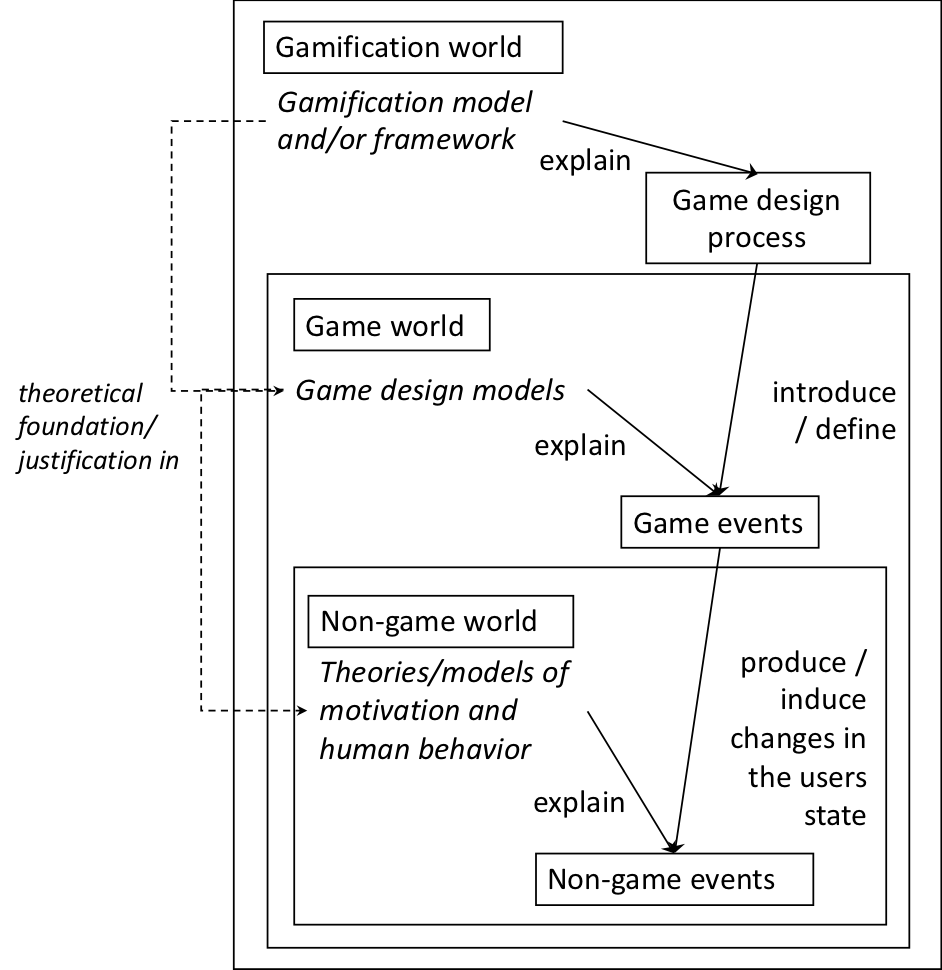
\includegraphics[width=0.55\textwidth]{images/chap-ontogacles2/nested-structure-game-nongame-worlds.png}
 \fautor
\end{figure}

Employing the nested-structure of non-game world, game world and gamification world (\autoref{fig:nested-structure-game-nongame-worlds}), the concepts in the ontology OntoGaCLeS related to the game events and non-game events have been classified in the \aspas{\emph{is-a}} hierarchy structure of class shown in \autoref{fig:is-a-hierarchy-structure-of-classes}.
This structure categorizes any concept of ontology as a sub-type of classes: \emph{Gamification world}, \emph{Game world}, Non-game world, Common world, and Theory/Model.
The classes defined under the categories of common, non-game, game and gamification worlds are concepts for things in their respective worlds, and the concepts formalized as sub-type of \emph{Theory/Model} define the theoretical foundation and justification of gamification and game design.

\emph{Gamification world} is the class of all things that depend of the gamification world to exist. In this sense, a concept is formalized as sub-type of \emph{Gamification world} whether it represents something that needs of gamification world to be described.
For instance, the \emph{Gamification goal/purpose} is a concept formalized as sub-type of Gamification world to describe the goals and/or purposes of a gamification model and/or framework (e.g. \emph{avoiding dropout}, \emph{reducing weariness}).
The basic concepts defined as sub-types of \emph{Gamification world} for the gamification of CL scenarios are: \emph{Gamified CL session}, \emph{Motivational strategy}  (\emph{Y<=I-mot goal}) by gamification, \emph{Player role}, and \emph{Individual gameplay strategy} (\emph{I-gameplay strategy}).

\emph{Game world} is the class of all things that depend of the game world to exist.
Concepts formalized as sub-types of \emph{Game world} require only elements defined in the games to be described.
The only basic concept defined as a sub-type of \emph{Game world} to gamify CL scenarios is: \emph{Game element}.
\emph{Non-game world} is the class of all things that do not need concepts from the \emph{Gamification world} or \emph{Game world} to exist.
The non-game world is divided in the sub-types: \emph{Learning world}, \emph{Instructional world}, \emph{World of cognition}, \emph{ID-ISD world}, \emph{CL world}, and \emph{World of motivation and human behavior}.
Basic concepts defined as one of these worlds respectively needs only things from its world to exist.
Thus, for instance, the concepts formalized as sub-types of\emph{ World of motivation and human behavio}r represent things that only need elements from motivation and human behavior to exist, so that the basic concepts related to the gamification of CL scenarios formalized as sub-types of \emph{World of motivation and human behavior} are: Individual motivational goal (\emph{I-mot goal}), \emph{Motivation stage}, and \emph{Human need stage}.

\emph{Common world} is the class of anything used to represent things that require concepts of other worlds to be formalized. These concepts are common to the other worlds, and they have been taxonomically classified taking as base the classification defined in the upper-level ontology \textbf{YAMATO} – \emph{\textbf{Y}et \textbf{A}nother \textbf{M}ore \textbf{A}dvanced \textbf{T}op-level \textbf{O}ntology} \cite{Mizoguchi2010}.
The basic concepts in the \emph{Common world} to represent persuasive game design are the concepts of: (i) \emph{action}, (ii) \emph{entity} (e.g. \emph{object}, \emph{agent}), (iii) \emph{state}, and (iv) \emph{event}.
These concepts, their sub-types, and their ontological structures have been formalized following the formalization proposed by Galton and Mizoguchi in the article \aspas{\emph{The Water Falls but the Waterfall Does Not Fall: New Perspectives on Objects, Processes and Events}} \cite{GaltonMizoguchi2009}.
According to these definitions, there is a mutual dependency between processes and entities whereby no one process (\emph{action}) can exist without an entity (\emph{agent} or \emph{object}) to enact it, and an entity is what it is as consequence of its processes.
Therefore, an entity has properties know as \emph{states} that change over time when processes are enacted by the object.
An \emph{event} is then defined as integration of entities, actions, and states in a particular context to delineate a fixed chunk of any process in which the participants of process are the agents and objects.

\begin{figure}[!htb]
 \caption{\aspas{\emph{is-a}} hierarchy structure of classes to represent concepts in the ontology OntoGaCLeS}
 \label{fig:is-a-hierarchy-structure-of-classes}
 \centering
 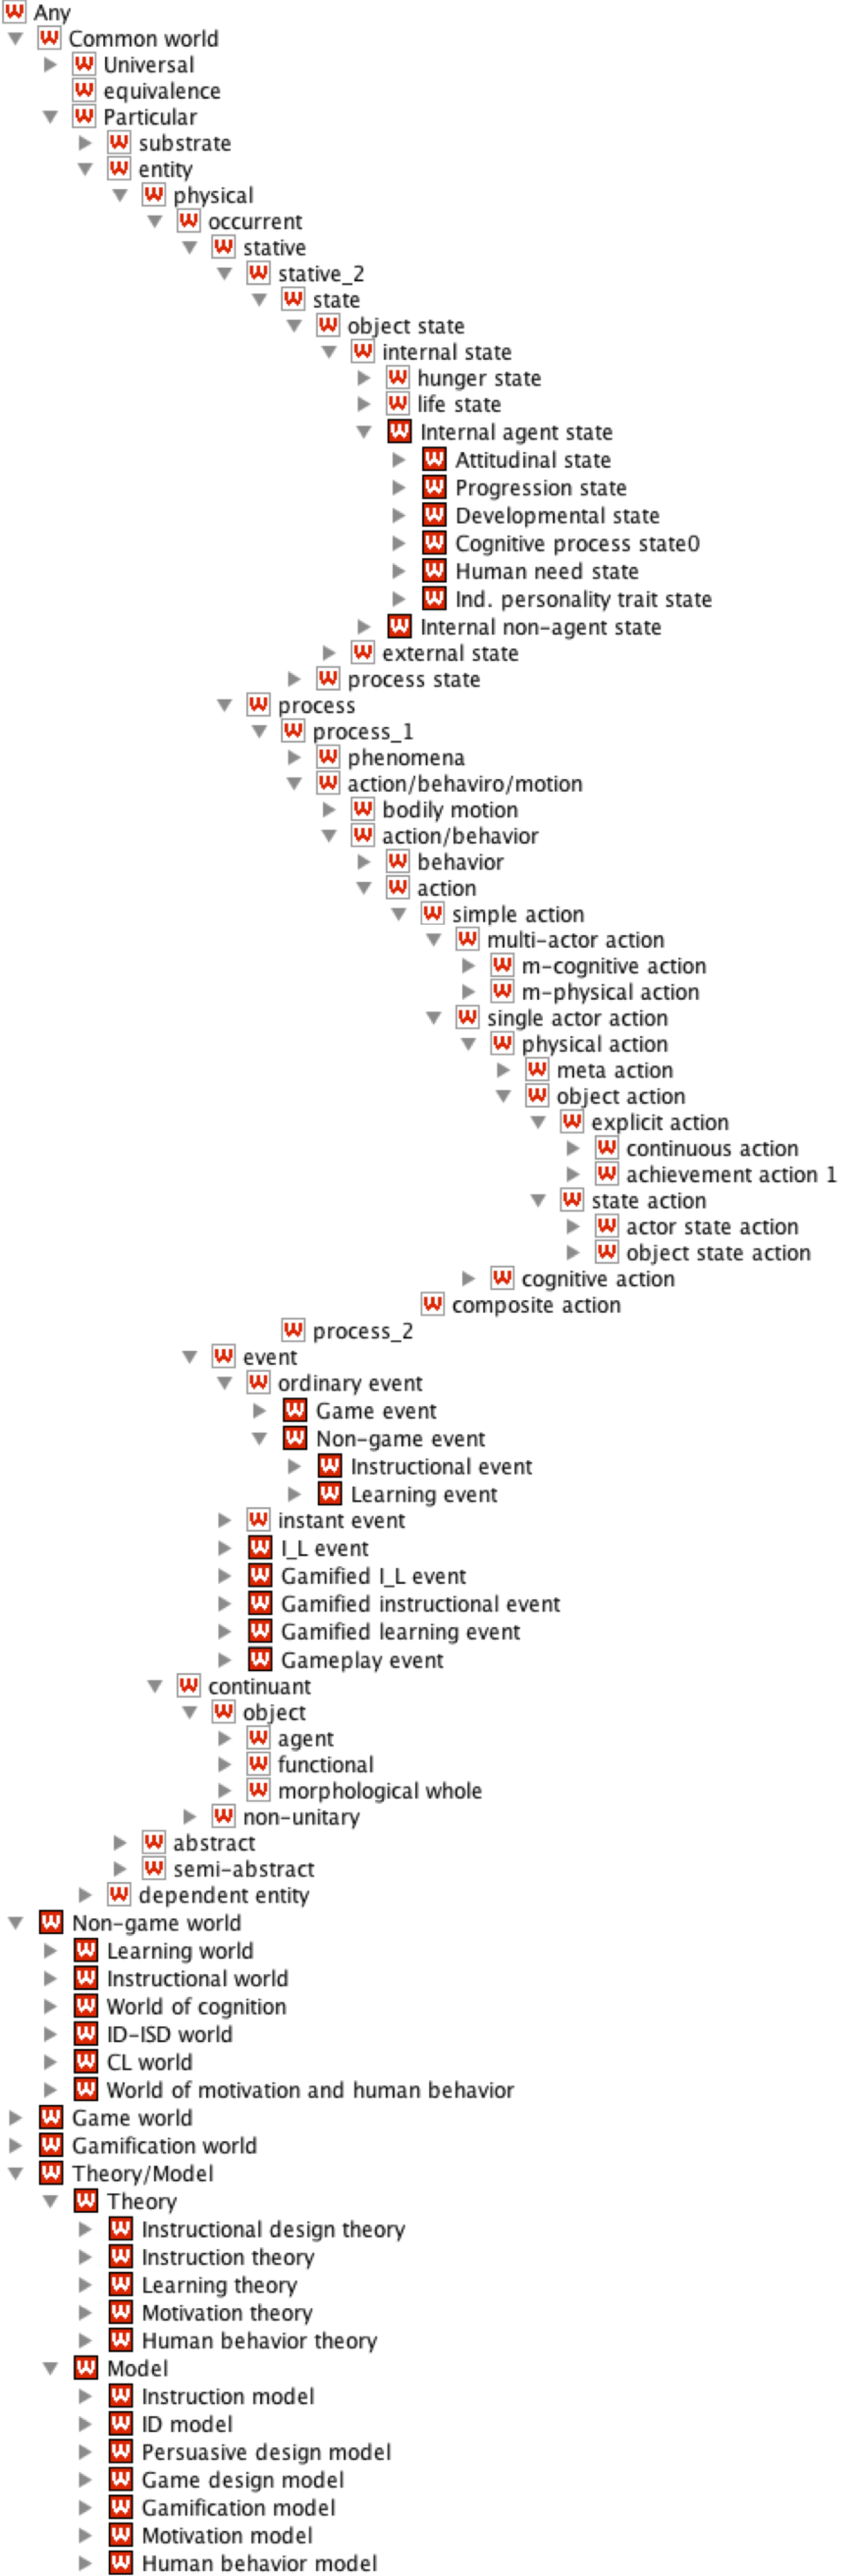
\includegraphics[width=0.46\textwidth]{images/chap-ontogacles2/is-a-hierarchy-structure-of-classes.png}
 \fautor
\end{figure}
\newpage

\autoref{fig:ontological-structures-event} shows the formalization of events as ontological structures in the ontology OntoGaCLeS.
As it has shown in this formalization, the class event is classified in \emph{ordinal event} and \emph{instant event} in which the ordinal event is constituted by a process (e.g. \emph{action}, \emph{behavior}), the participants in the events are entities, and the ordinal event has instantaneous events as starting and ending event to delimit the chunk of processes that compose the event. 
Finally, the \emph{ordinal event} is divided in two sub-types: \emph{Game event} and \emph{Non-game event} - as shown in the \aspas{\emph{is-a}} hierarchy of classes (\autoref{fig:is-a-hierarchy-structure-of-classes}).
The composed events in the \aspas{\emph{is-a}} hierarchy structure of classes are defined as subtype of \emph{event}, and they are: \emph{I\_L event}, \emph{Gameplay event}, \emph{Gamified Instructional event}, \emph{Gamified Learning event}, and \emph{Gamified I\_L event}.
The formalization as ontological structures of these events is detailed in the following sections.

\begin{figure}[!htb]
 \caption{Ontological structures to represent events}
 \label{fig:ontological-structures-event}
 \centering
 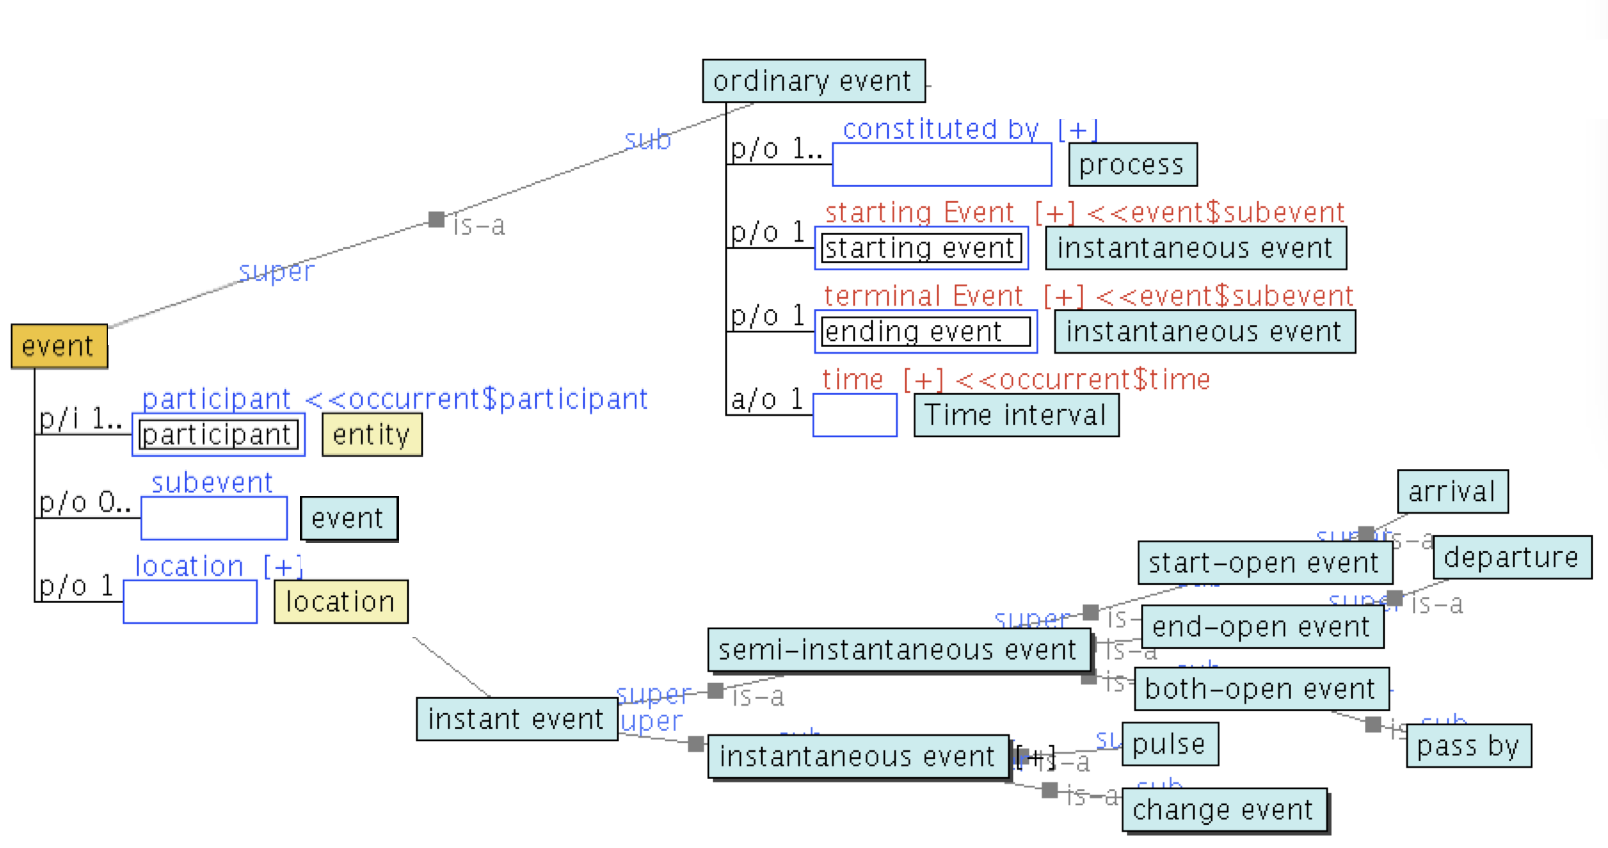
\includegraphics[width=1\textwidth]{images/chap-ontogacles2/ontological-structures-event.png}
 \fautor
\end{figure}

%%%%%%%%%%%%%%%%%%%%%%%%%%%%%%%%%%%%%%%%%%%%%%%%%%
\section[Modeling Persuasive Game Design]{Modeling Persuasive Game Design}
\label{sec:modeling-persuasive-game-design}

\emph{Persuasive Game Design} (PGD) is defined as \aspas{\emph{the game design for the purpose to change peoples’ attitudes, intentions, motivations and/or behaviors through persuasion and social influence without using coercion and/or deception}.}
In this sense, to represent the PGD as ontological structures, an ontology-based formalization of the \emph{game design} is needed because PGD is conceptualized as a game design that is embedded in persuasive design.

As was explained in the previous section, game design models are used to define the game events whereby the changes in the users’ states are produced or induced in a non-game events, and these changes are explained by theories/models of motivation a human behavior.
Therefore, the game design consists into establish the relation between non-game event and game event based on theoretical justification extracted from game design models and theories of motivation and human behavior.
When this game design has the purpose is to change the participants' attitudes intentions, motivations, or behaviors becomes PGD, and it has been formalized in the ontology OntoGaCLeS as ontological structures to represent the \emph{persuasive gameplay event} and the \emph{WAY-knowledge of PGDS} detailed in \autoref{subsec:persuasive-gameplay-event} and \autoref{subsec:way-knowledge-of-persuasive-game-design}.
Employing the ontology-based formalization of PGD, the concept of \aspas{\emph{Persuasive Gameplay Scenario Model}} has been proposed to represent the design rationale of how to apply PGD in non-game events.
The formalization of this model as ontological structures is presented in \autoref{subsec:persuasive-gameplay-scenario-model}.

\subsection{Persuasive Gameplay Events}
\label{subsec:persuasive-gameplay-event}

The PGD is explicitly represented as the relation between game events and non-game events in the ontology OntoGaCLeS under the concept of \emph{Gameplay event}.
This concept describes, in an explicit way, what happens in the non-game world and the game world when the user is persuaded and/or socially influenced to interacts with the system.
Thus, a \emph{Persuasive gameplay event} is formalized as an explicit description of the relation between game events and a non-game event in which the doer of the non-game event has been persuaded and/or socially influenced by the game events.

\autoref{fig:ontological-structures-persuasive-gameplay-events} shows the ontological structures proposed to represent persuasive gameplay events, where the \emph{Gameplay event} (at the top of figure) represents any interaction that would occur between the participants and the game elements in the system that is being gamified.
In the formalization of gameplay event, the \emph{Game event} describes actions performed by an \emph{agent} that becomes \emph{Game agent}, an \emph{action} of this agent becomes \emph{Game action}, the \emph{participant} who interacts with the game agent becomes \emph{Player}, and the object produced as consequence of \emph{Game action} becomes a \emph{Game component}.

\begin{figure}[!htb]
 \caption[Ontological structures to represent persuasive gameplay events]{Ontological structures to represent persuasive gameplay events. \aspas{\emph{Gameplay event}} at the top, \aspas{\emph{Gameplay-stimulus event}} at the bottom-left, \aspas{\emph{Gameplay-mechanism event}} at the bottom-center, and \aspas{\emph{Gameplay-consequence event}} at the bottom-right.}
 \label{fig:ontological-structures-persuasive-gameplay-events}
 \centering
 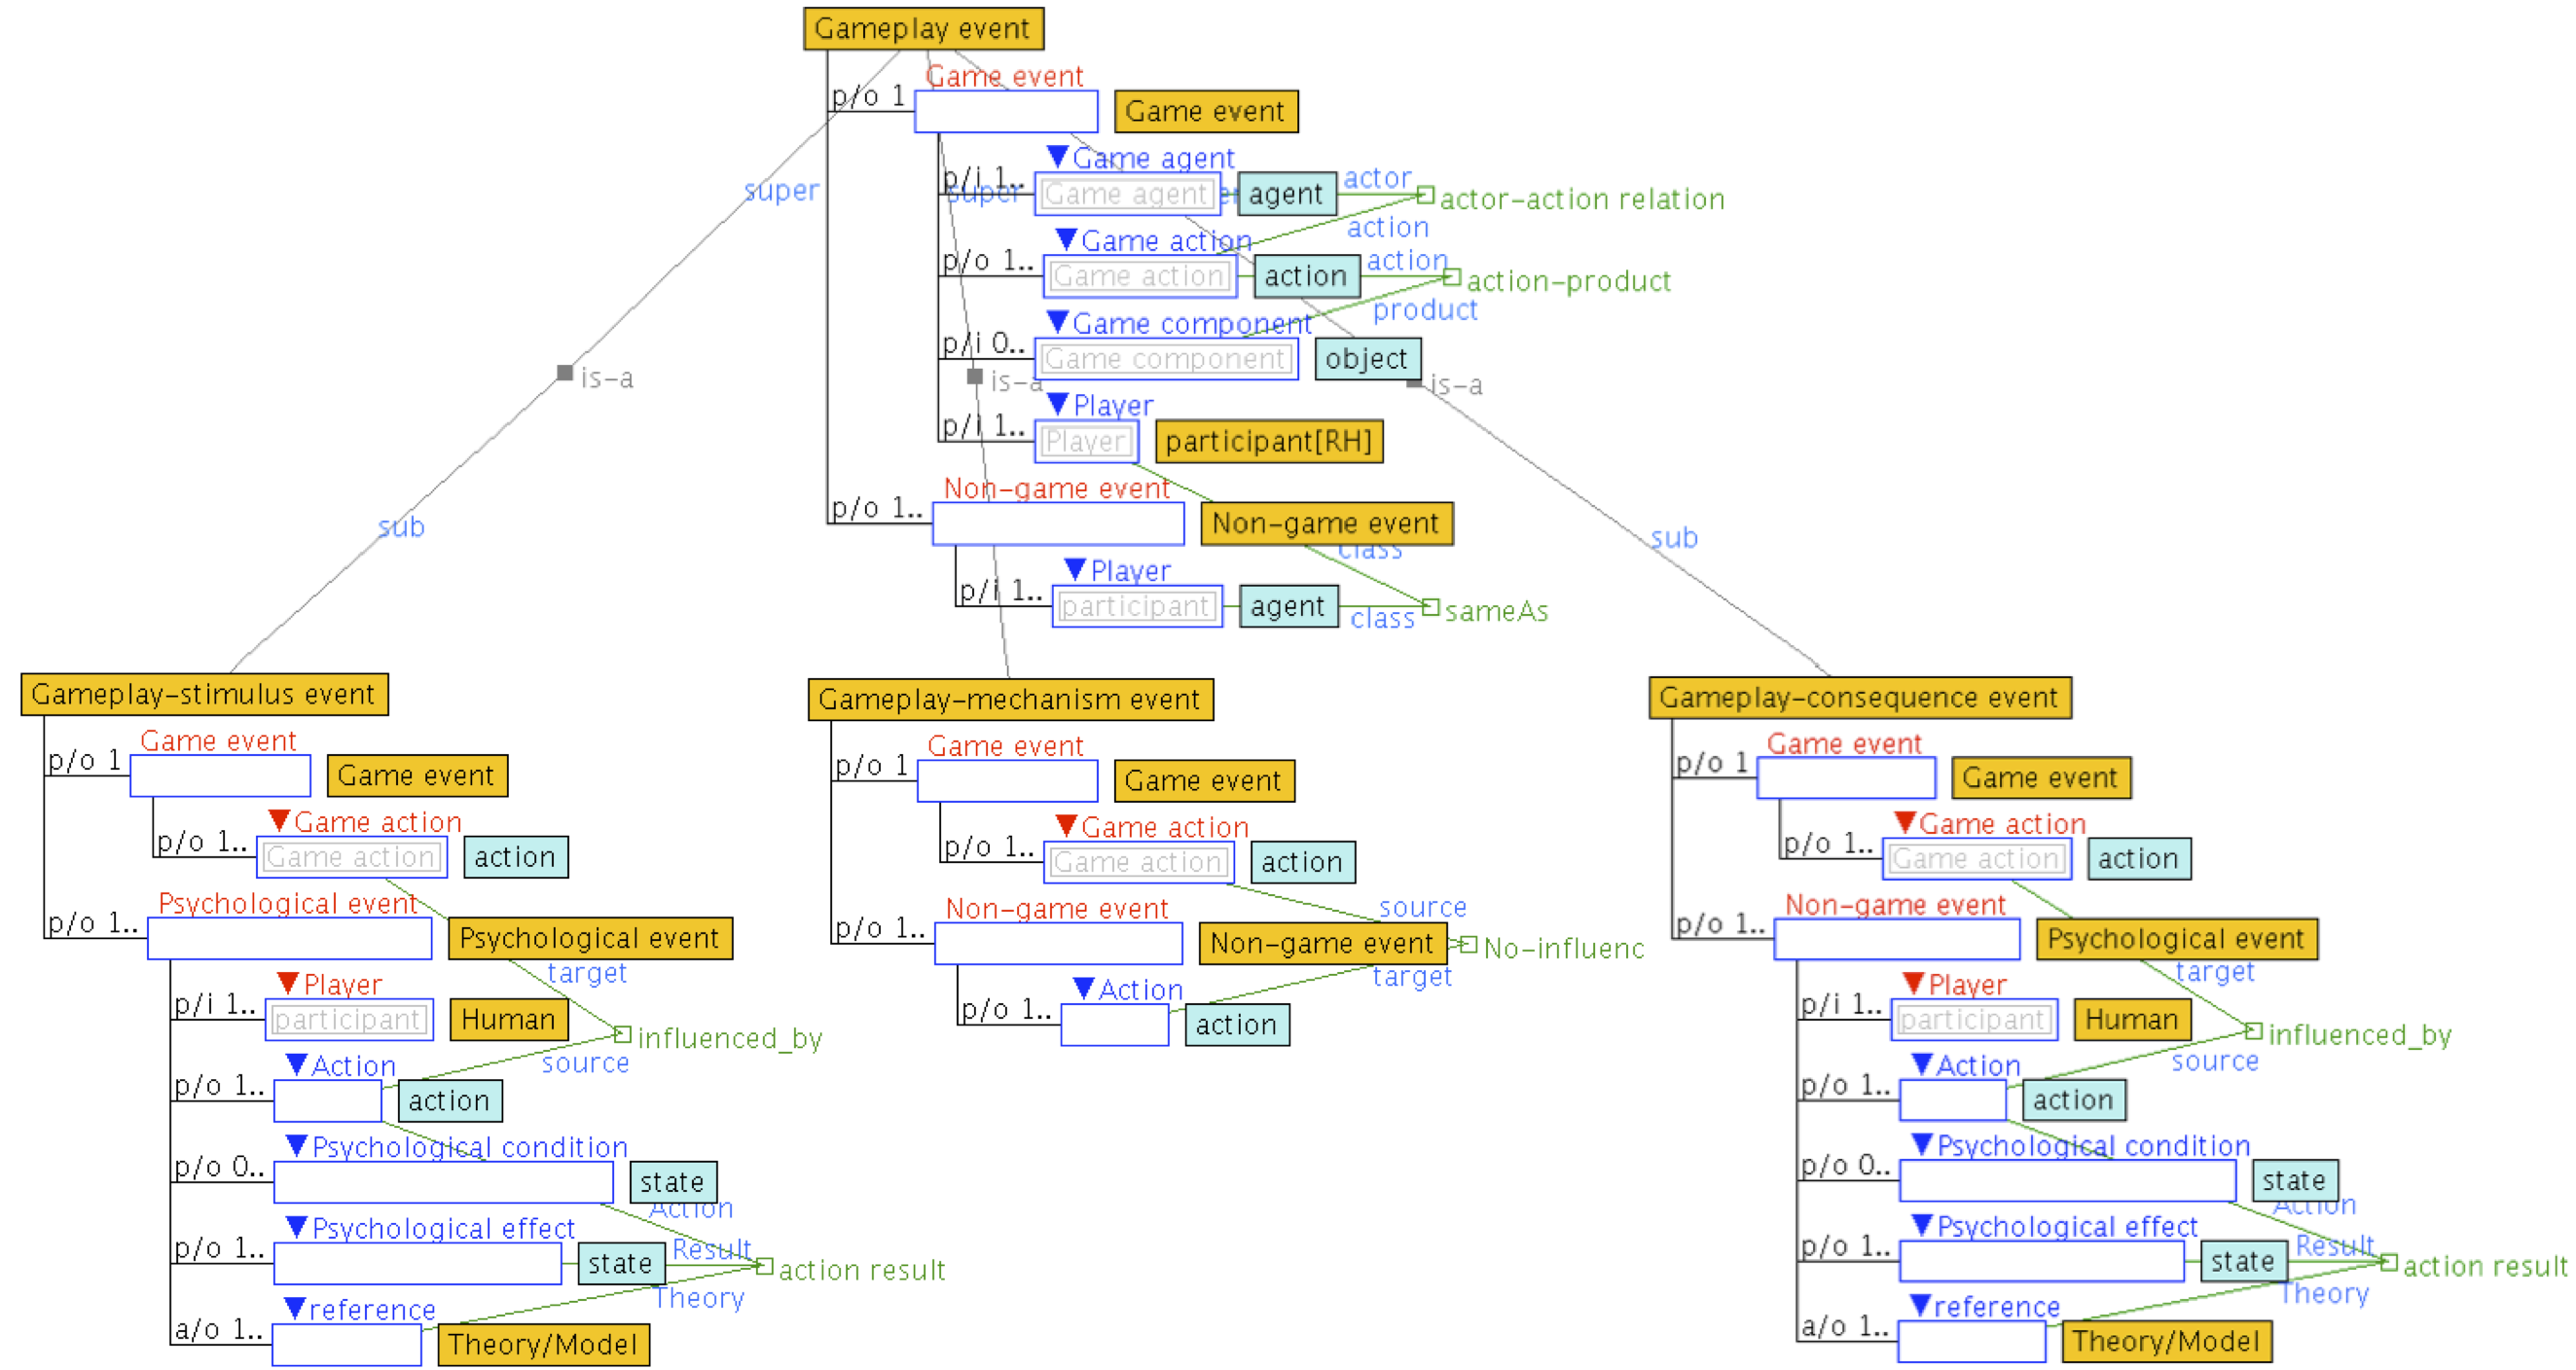
\includegraphics[width=1\textwidth]{images/chap-ontogacles2/ontological-structures-persuasive-gameplay-events.png}
 \fautor
\end{figure}

When game events are used to lead the participants into take actions by persuasion and/or social influence, there are three types of interactions defined as persuasive game events.
These events are: \emph{Gameplay-stimulus event}, \emph{Gameplay-mechanism event}, and \emph{Gameplay-consequence event}.
The gameplay-stimulus and gameplay-consequence events are used to represent internal psychological processes that occur by influence of a game action, whereas the gameplay-mechanism event has been formalized to represent actions that occur in the non-game world.
In a \emph{Gameplay-stimulus event}, the game actions occur before the actions being gamified, and, in a \emph{Gameplay-consequence event}, the game actions occur after the actions being gamified.
These both gameplay events are formalized as ontological structures showed at the bottom-left and bottom-right of \autoref{fig:ontological-structures-persuasive-gameplay-events}, where the internal psychological process associated to game actions is represented as a pair of events: \emph{Game event} and \emph{Psychological event}.
In these formalizations, the \emph{action} of the \emph{Psychological event} is \emph{influenced by} the action defined as \emph{Game action} in the \emph{Game event}.
Concepts of \emph{state} are used in the psychological event to represent \emph{Psychological condition} and \emph{Psychological effect} related to the participants' changes of attitudes, intentions, motivations and/or behaviors.
These changes, in the ontological structures, are explained by theories and models of motivation and human behavior (\emph{Theory/Model}) derived and/or related to persuasion and social influence, such as classical conditioning \cite{GormezanoProkasyThompsonThompson1987}, operant conditioning \cite{Skinner1953}, and Fogg's behavior model \cite{Fogg2009}.

To illustrate the use of the ontological structures presented in \autoref{fig:ontological-structures-persuasive-gameplay-events}, let us formally represent the gameplay events that occur when \aspas{\emph{a participant is persuaded to obtain points by making a comment in a post}} illustrated as a storyboard shown at the top of \autoref{fig:ontological-structures-example-persuasive-gameplay-events}.
This storyboard as ontological structures is formalized at the bottom of \autoref{fig:ontological-structures-example-persuasive-gameplay-events}, where \emph{Raising motivation by promising points event} is represented as gameplay-stimulus event, the \emph{Comment post event} is represented as gameplay-mechanism event, and the \emph{Increasing behavior by giving points event} is represented as gameplay-consequence event.
The game action \aspas{\emph{Promise points}} and the internal psychological process \aspas{\emph{Raise motivation}} are represented as the game-stimulus event \aspas{\emph{Raising motivation by promising points event}} shown at the left of figure.
According to this structure, the psychological effect is being \emph{Motivated}, and the condition to achieve this state is being \emph{Not motivated}. This change of state is explained by the Foog's behavior model \cite{Fogg2009}.
The game-mechanism event with the \emph{Comment post event} as the non-game event being gamified is shown at the center of figure, and it describes the action of \emph{Comment post} performed by the participant in a non-game system.
The \emph{Increasing behavior by giving points event} at the right of figure is a gameplay-consequence event in which the action \aspas{\emph{Increase self-behavior}} is \emph{influenced by} the game action \aspas{\emph{Give points}} performed by a \emph{Point system}.
The Foog's behavior grid model explains the change described in the psychological event in which the psychological condition is \emph{Being non-familiar behavior} and the psychological effect is \emph{Being familiar behavior}.

\begin{figure}[!htb]
 \caption[Example of ontological structures to represent persuasive gameplay events]{Example of ontological structures to represent persuasive gameplay events in which  \aspas{\emph{a participant is persuaded to obtain points by making a comment in a post}} (at the bottom). At the top, the storyboard of gameplay events involved in this example.}
 \label{fig:ontological-structures-example-persuasive-gameplay-events}
 \centering
 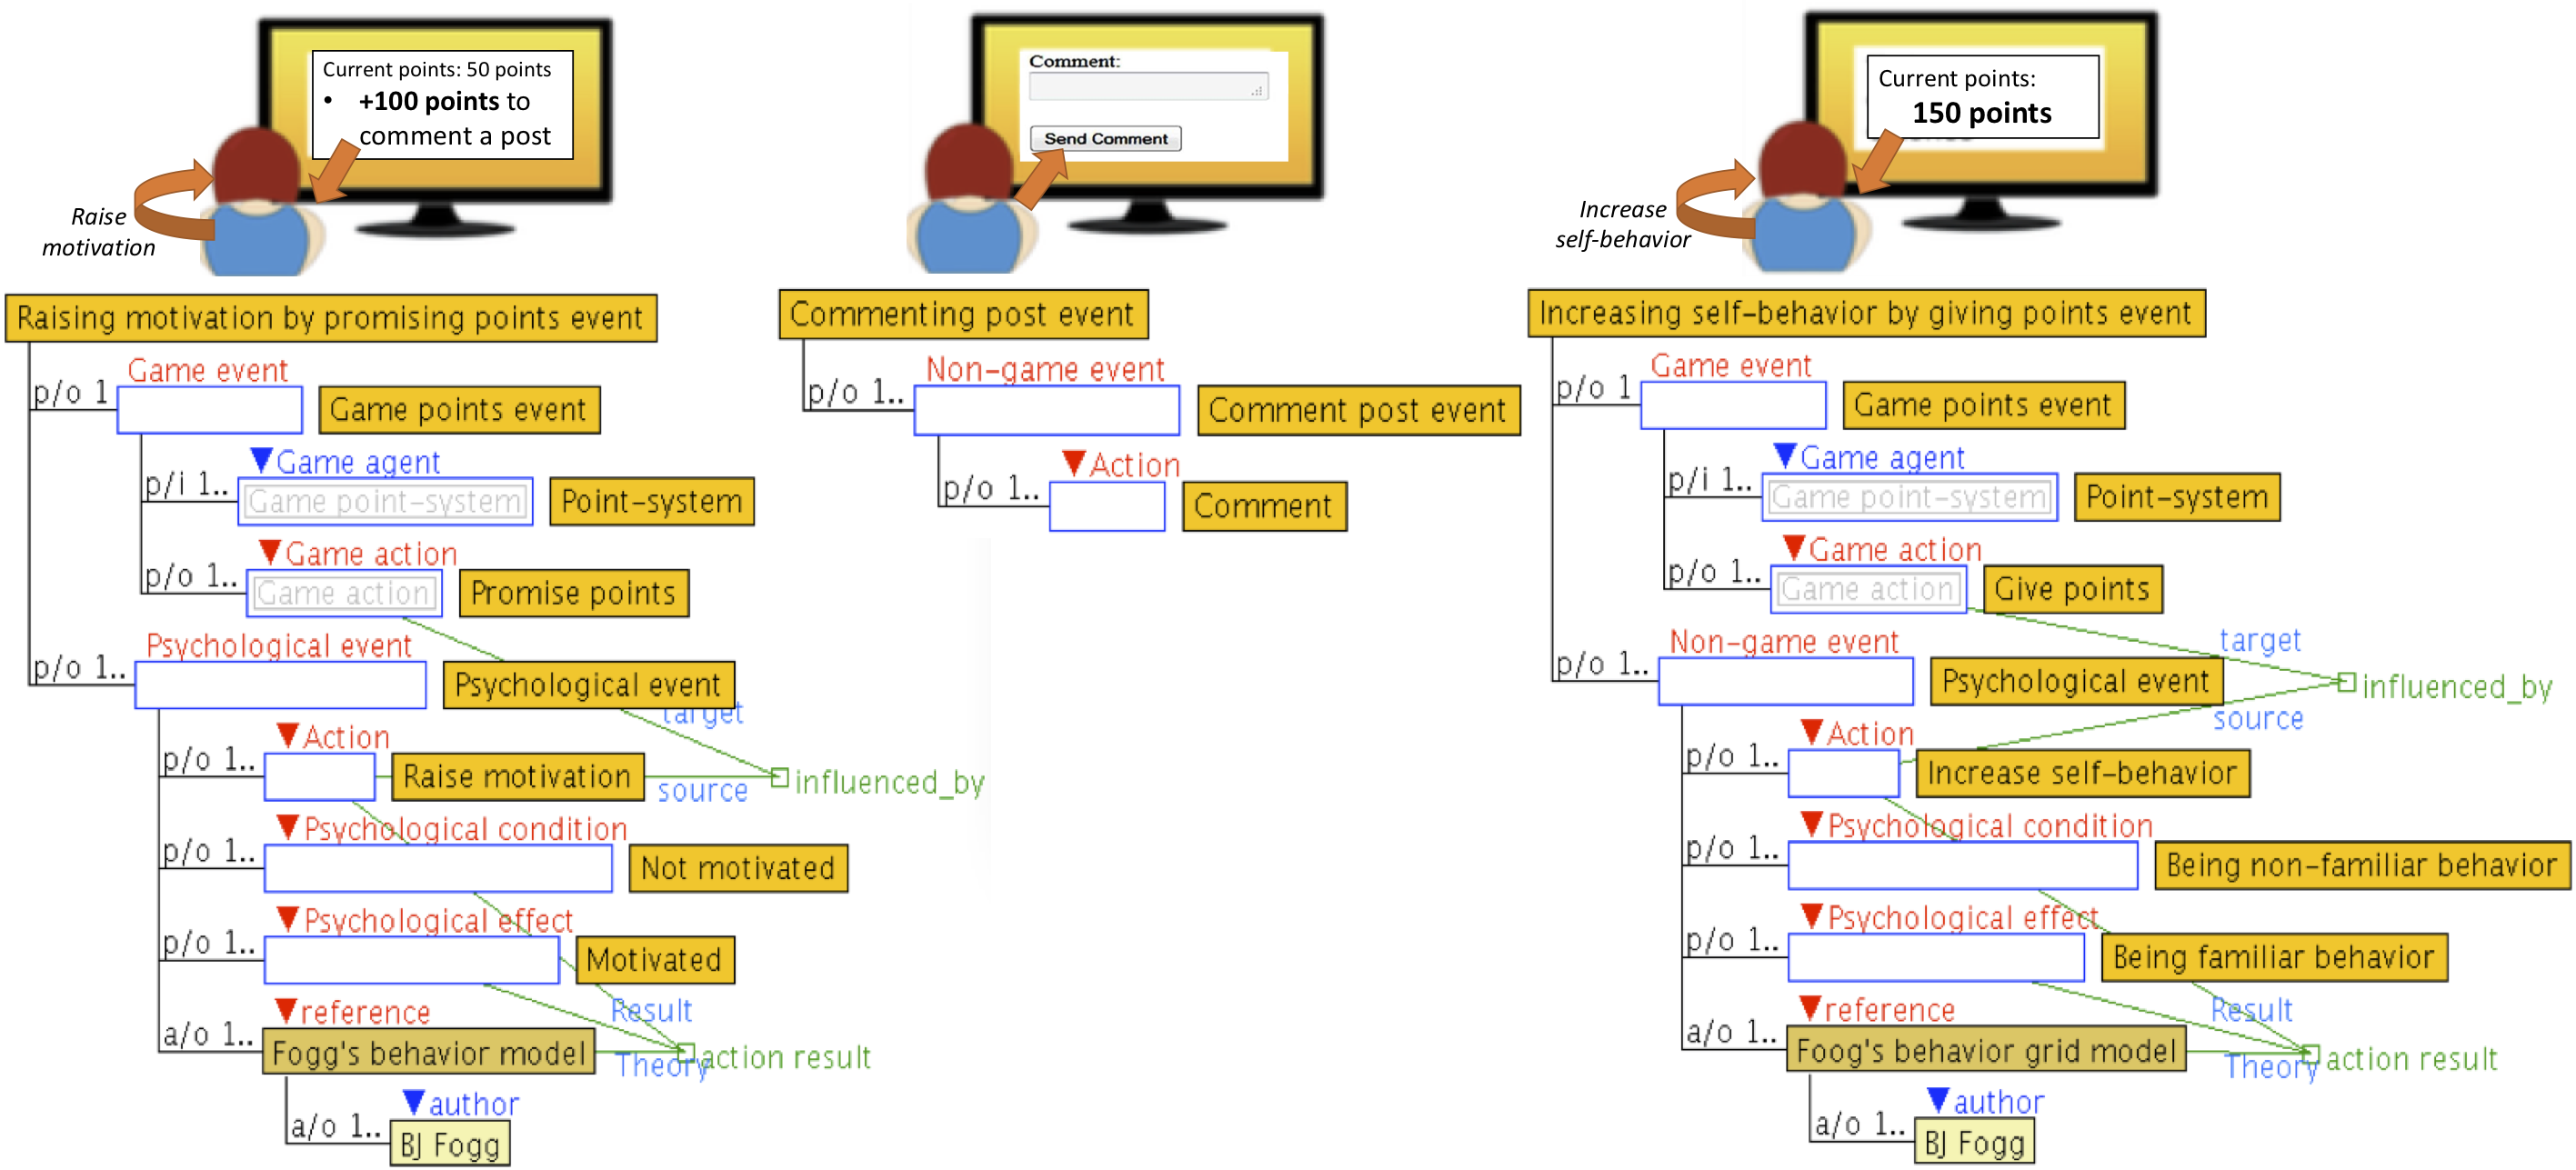
\includegraphics[width=1\textwidth]{images/chap-ontogacles2/ontological-structures-example-persuasive-gameplay-events.png}
 \fautor
\end{figure}

\subsection{WAY-knowledge of PGDS}
\label{subsec:way-knowledge-of-persuasive-game-design}

\emph{WAY-knowledge of PGDS} is a prescriptive description of PGD in which the relation between game events and non-game events is defined as a decomposition method of gameplay events.
Thus, to describe how to achieve a specific change in the participants' attitudes and attitudes, intentions, motivations and/or behaviors, a gameplay event can be broken down into several gameplay-event sequences.
The strategy of choosing a decomposition method to be applied in gameplay-event is known as \emph{Game Design Strategy} (GDS), and when it is performed according to persuasive principles, it is known as \emph{Persuasive Game Design Strategy} (PGDS).

PGDSs are game design strategies that are embedded in persuasive strategies, and their representation as \emph{WAY-knowledge} constitutes a game design with the dedicate function to persuade and/or to cause social influence in the participants of non-game events.
Therefore, the formalization of the knowledge involved in the PGDSs has been defined in the ontology OntoGaCLeS as a simplified version of the \emph{WAY-structure} proposed by \citeonline{KitamuraMizoguchi2004,KitamuraKashiwaseFuseMizoguchi2004} to represent functions.
The simplified version of the \emph{WAY-structure} has been formalized  as the ontological structure\aspas{\emph{WAY-knowledge}} showed at the top of \autoref{fig:ontological-structures-way-knowledge-of-pgds} in which the sequence of \emph{micro}-events represents the way to accomplish the \emph{macro}-event.
This decomposition, known as way knowledge, is theoretical grounded in a \emph{Theory/Model} delineated as attribute \aspas{\emph{Theory for reference}} in the ontological structure to represent the \emph{WAY-knowledge}.

\begin{figure}[!htb]
 \caption[Ontological structures to represent \emph{WAY-knowledge of PGDS}]{Ontological structures to represent \aspas{\emph{WAY-knowledge of PGDS}.}}
 \label{fig:ontological-structures-way-knowledge-of-pgds}
 \centering
 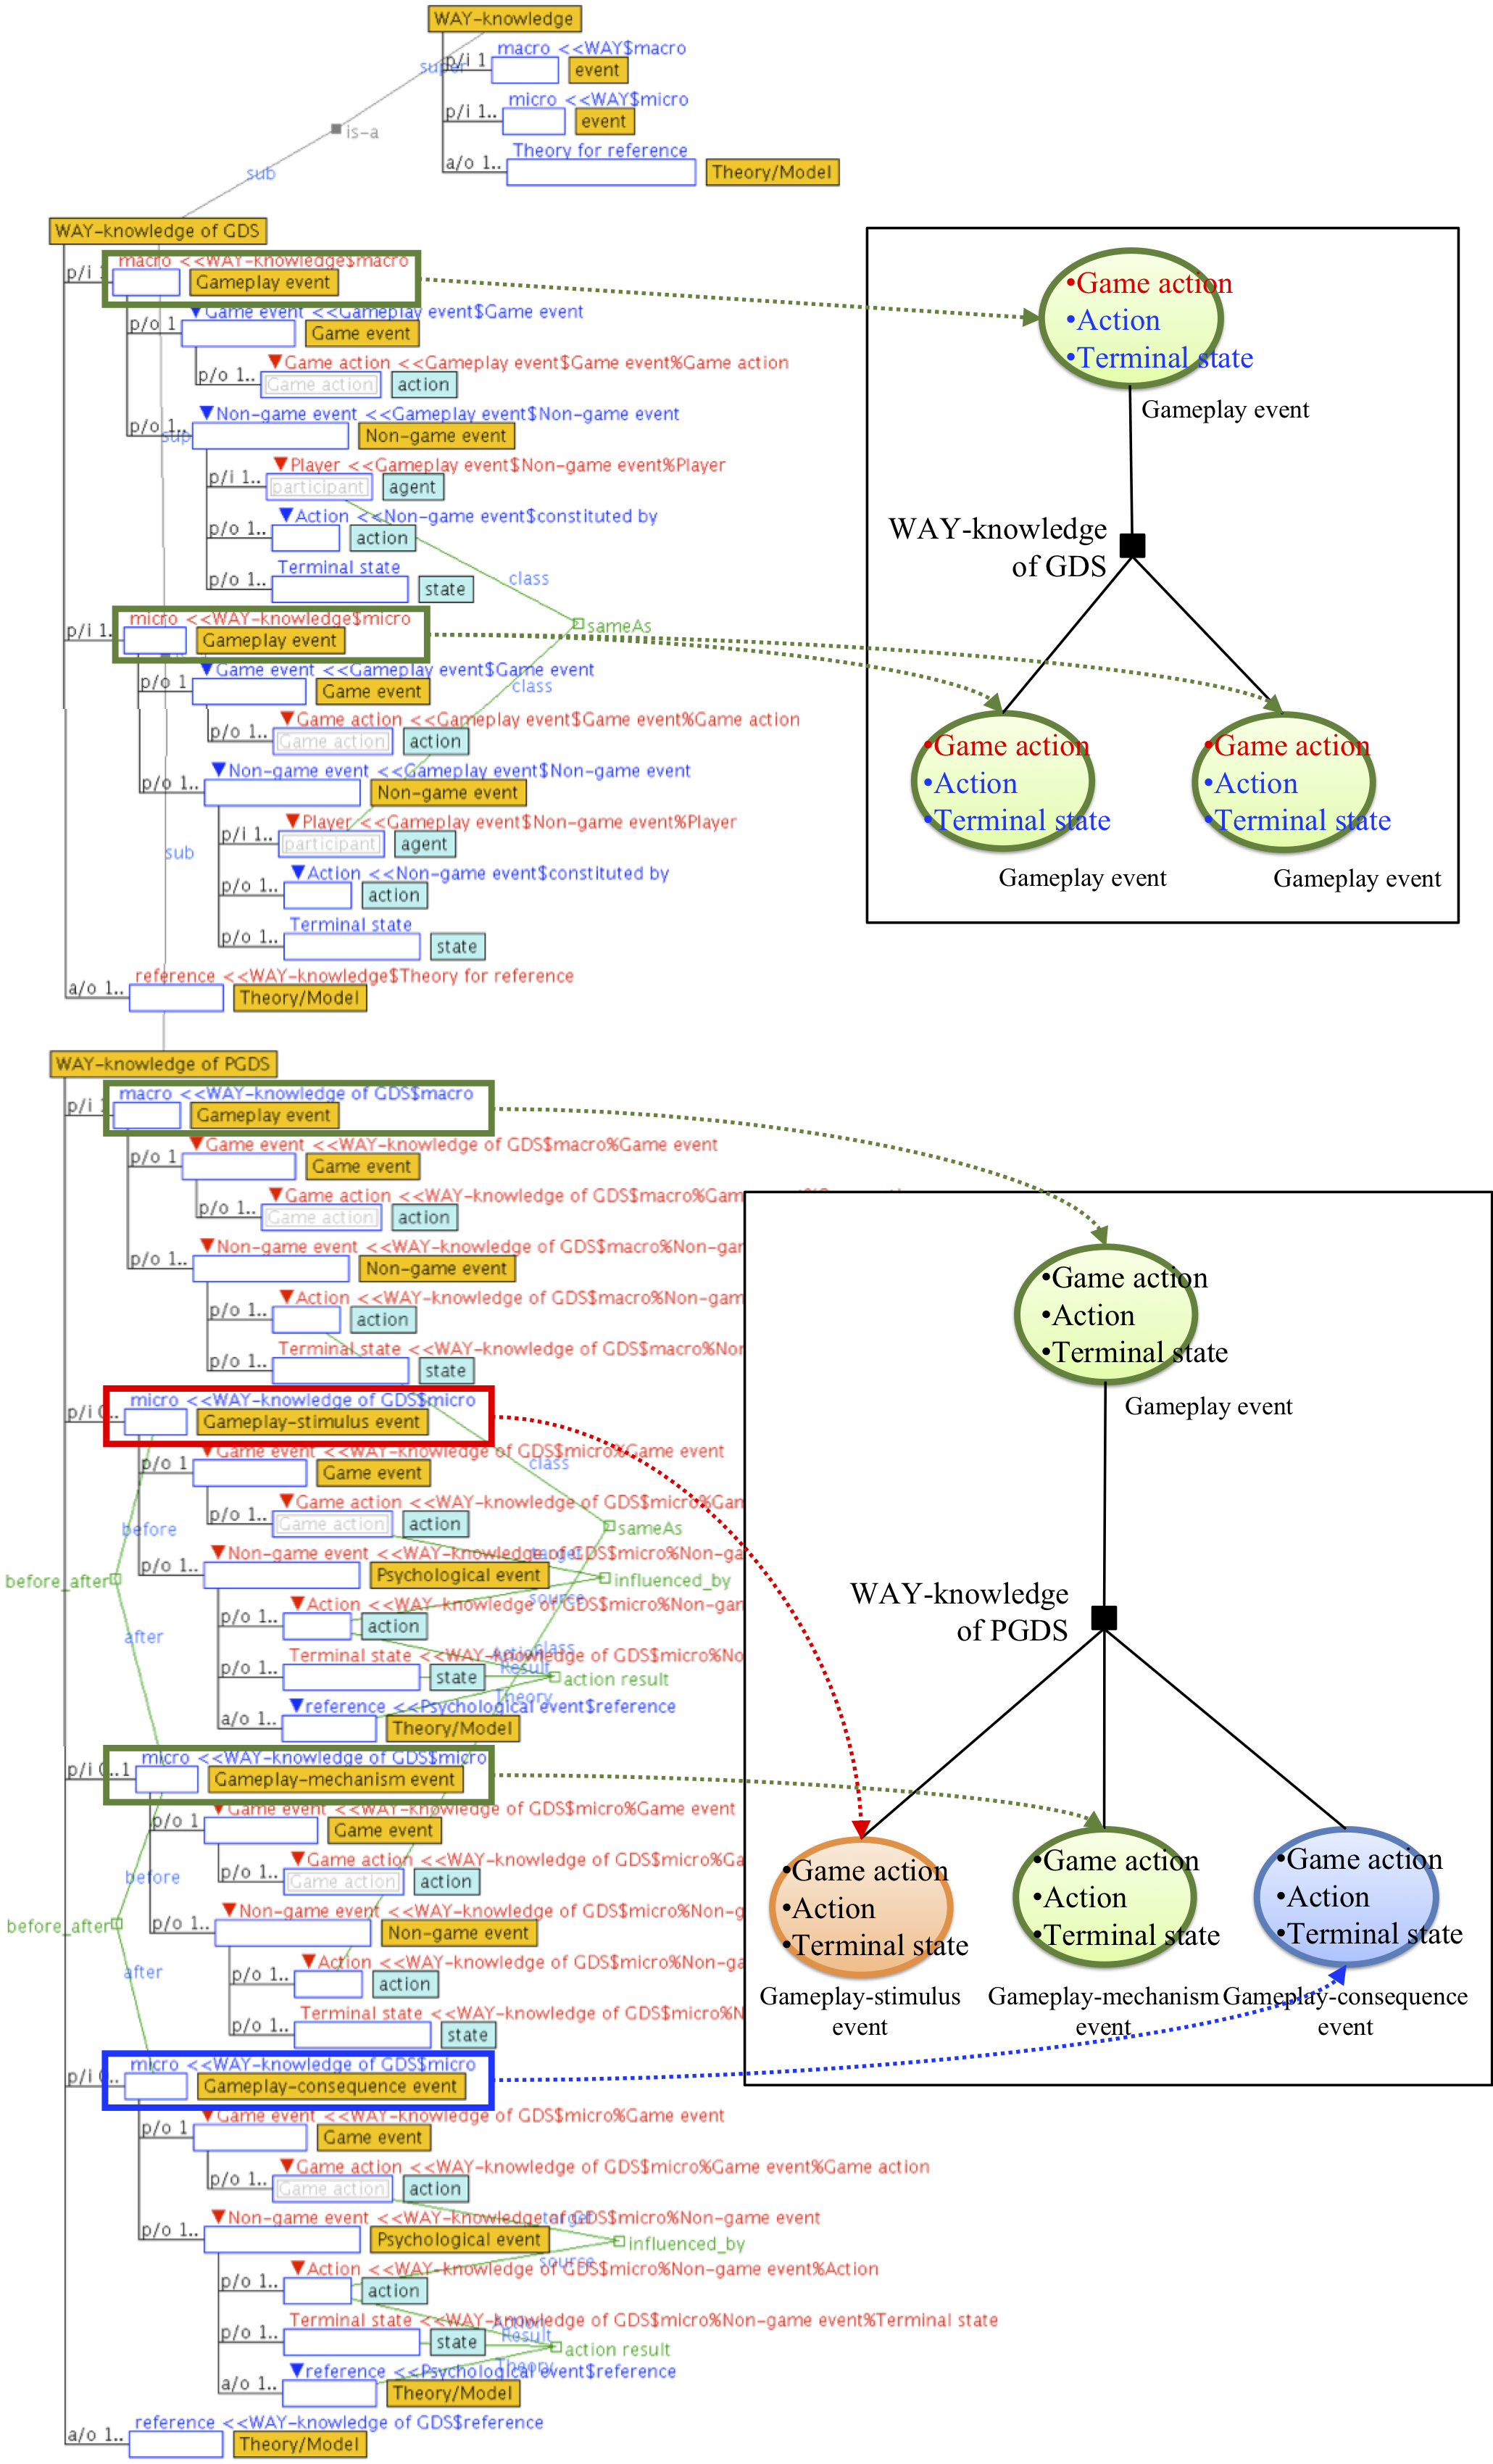
\includegraphics[width=0.84\textwidth]{images/chap-ontogacles2/ontological-structures-way-knowledge-of-pgds.png}
 \fautor
\end{figure}
\newpage

On the left side of the \autoref{fig:ontological-structures-way-knowledge-of-pgds}, the way knowledge about how to engender a contemplated terminal state in the player through his/her interaction with game elements is formalized as the ontological structure \aspas{\emph{WAY-knowledge of GDS}.}
This ontological structure is a prescriptive description of the game design in which the decomposition tree shown at the right side of the figure indicates that the \emph{Terminal state} in the \emph{macro}-gameplay event is achieved by a sequence of \emph{micro}-gameplay events.
The way knowledge about how to achieve contemplated change in participants' attitudes, intentions, motivations and/or behaviors through interaction with the game elements are represented as the ontological structure \aspas{\emph{WAY-knowledge of PGDS}} shown on the left side of the figure. 
This structure represents the relation between game events and non-game events as the decomposition method of a \emph{macro}-gameplay event into a sequence of \emph{Gameplay-stimulus events}, \emph{Gameplay-mechanism events} and \emph{Gameplay-consequence events} as shown in the decomposition tree shown on the right side of the figure.
According to this ontological structure, the \emph{Terminal state} in the \emph{macro}-gameplay event represents \aspas{\emph{what to achieve}} as the goal of decomposition method, and the terminal states in the \emph{micro}-gameplay events represent \aspas{\emph{how to achieve}} this goal as a sequence of sub-goals to be achieved by the \emph{micro}-gameplay events.
The goals and sub-goals as terminal states are the result of actions performed by the participants in the non-game events, and when these actions are part of an internal psychological process (e.g raising motivation, increase self-behavior) influenced by game actions defined in the game events, the \emph{micro}-gameplay event is a \aspas{\emph{Gameplay-stimulus event}} or a \aspas{\emph{Gameplay-consequence event}.}
The decomposition method is theoretically justified on \emph{Theory/Model} that is \emph{reference} as an \emph{attribute-of} in the ontological structure to represent \aspas{\emph{WAY-knowledge of PGDS}.}

Based on the ontological structures to represent \aspas{\emph{WAY-knowledge of PGDS}} (\autoref{fig:ontological-structures-way-knowledge-of-pgds}), a WAY-knowledge base of GDSs and PGDSs has been defined in the ontology OntoGaCLeS. Part of this base is shown in \autoref{fig:portion-way-knowledge-base-pgds}, where the PGDSs were formalized based on the Persuasive System Design (PSD) proposed by \citeonline{Oinas-KukkonenHarjumaa2009}.
These PGDSs were firstly classified according to the categories of persuasive principles, and secondly, according to the contemplated changes in the participants' states.
The decomposition trees of two PGDSs are shown in this figure in which the PGDS \aspas{\emph{Reward strategy to be motivated and to make familiar behavior based on PSD}} has been classified as a \emph{Reward strategy} in the \emph{PGDS for dialogue}, and the PGDS \aspas{\emph{Suggestion strategy to be attentive based on PSD}} has been classified as \emph{Suggestion strategy} in the \emph{PGDS for dialog}.
The PGDS \aspas{\emph{Reward strategy to be motivated and to make familiar behavior based on PSD}} decomposes the \emph{macro}-gameplay event into three \emph{micro}-gameplay events defined by the game actions: \emph{Promise reward}, \emph{Await}, and \emph{Give reward}. During the gameplay-stimulus event defined by the game action \aspas{\emph{Promise reward},} the internal psychological process is \emph{Raise motivation} to achieve the \emph{Terminal state} \aspas{being \emph{Motivated}.} For the gameplay-consequence event defined by the game action \aspas{\emph{Give reward},} the internal psychological process is \emph{Increase self-behavior} to achieve the \emph{Terminal state} \aspas{\emph{Being familiar behavior}.}
The decomposition tree of the PGDS \aspas{\emph{Suggestion strategy to be attentive based on PSD}} indicates that, to achieve the \emph{Terminal state} of \emph{Being attentive}, it is necessary to follow the sequence of two \emph{micro}-gameplay events defined by the game actions \aspas{\emph{Give suggestion}} and \aspas{\emph{Await}.}
The internal psychological process \aspas{\emph{Focus attention}} in the gameplay-stimulus even is influenced by the game action \aspas{\emph{Give suggestion}} achieving the \emph{Terminal state} \aspas{\emph{Being attentive}.}

\begin{figure}[!htb]
 \caption{A portion of the WAY-knowledge base of game design strategies and persuasive game design strategies defined in the ontology OntoGaCLeS}
 \label{fig:portion-way-knowledge-base-pgds}
 \centering
 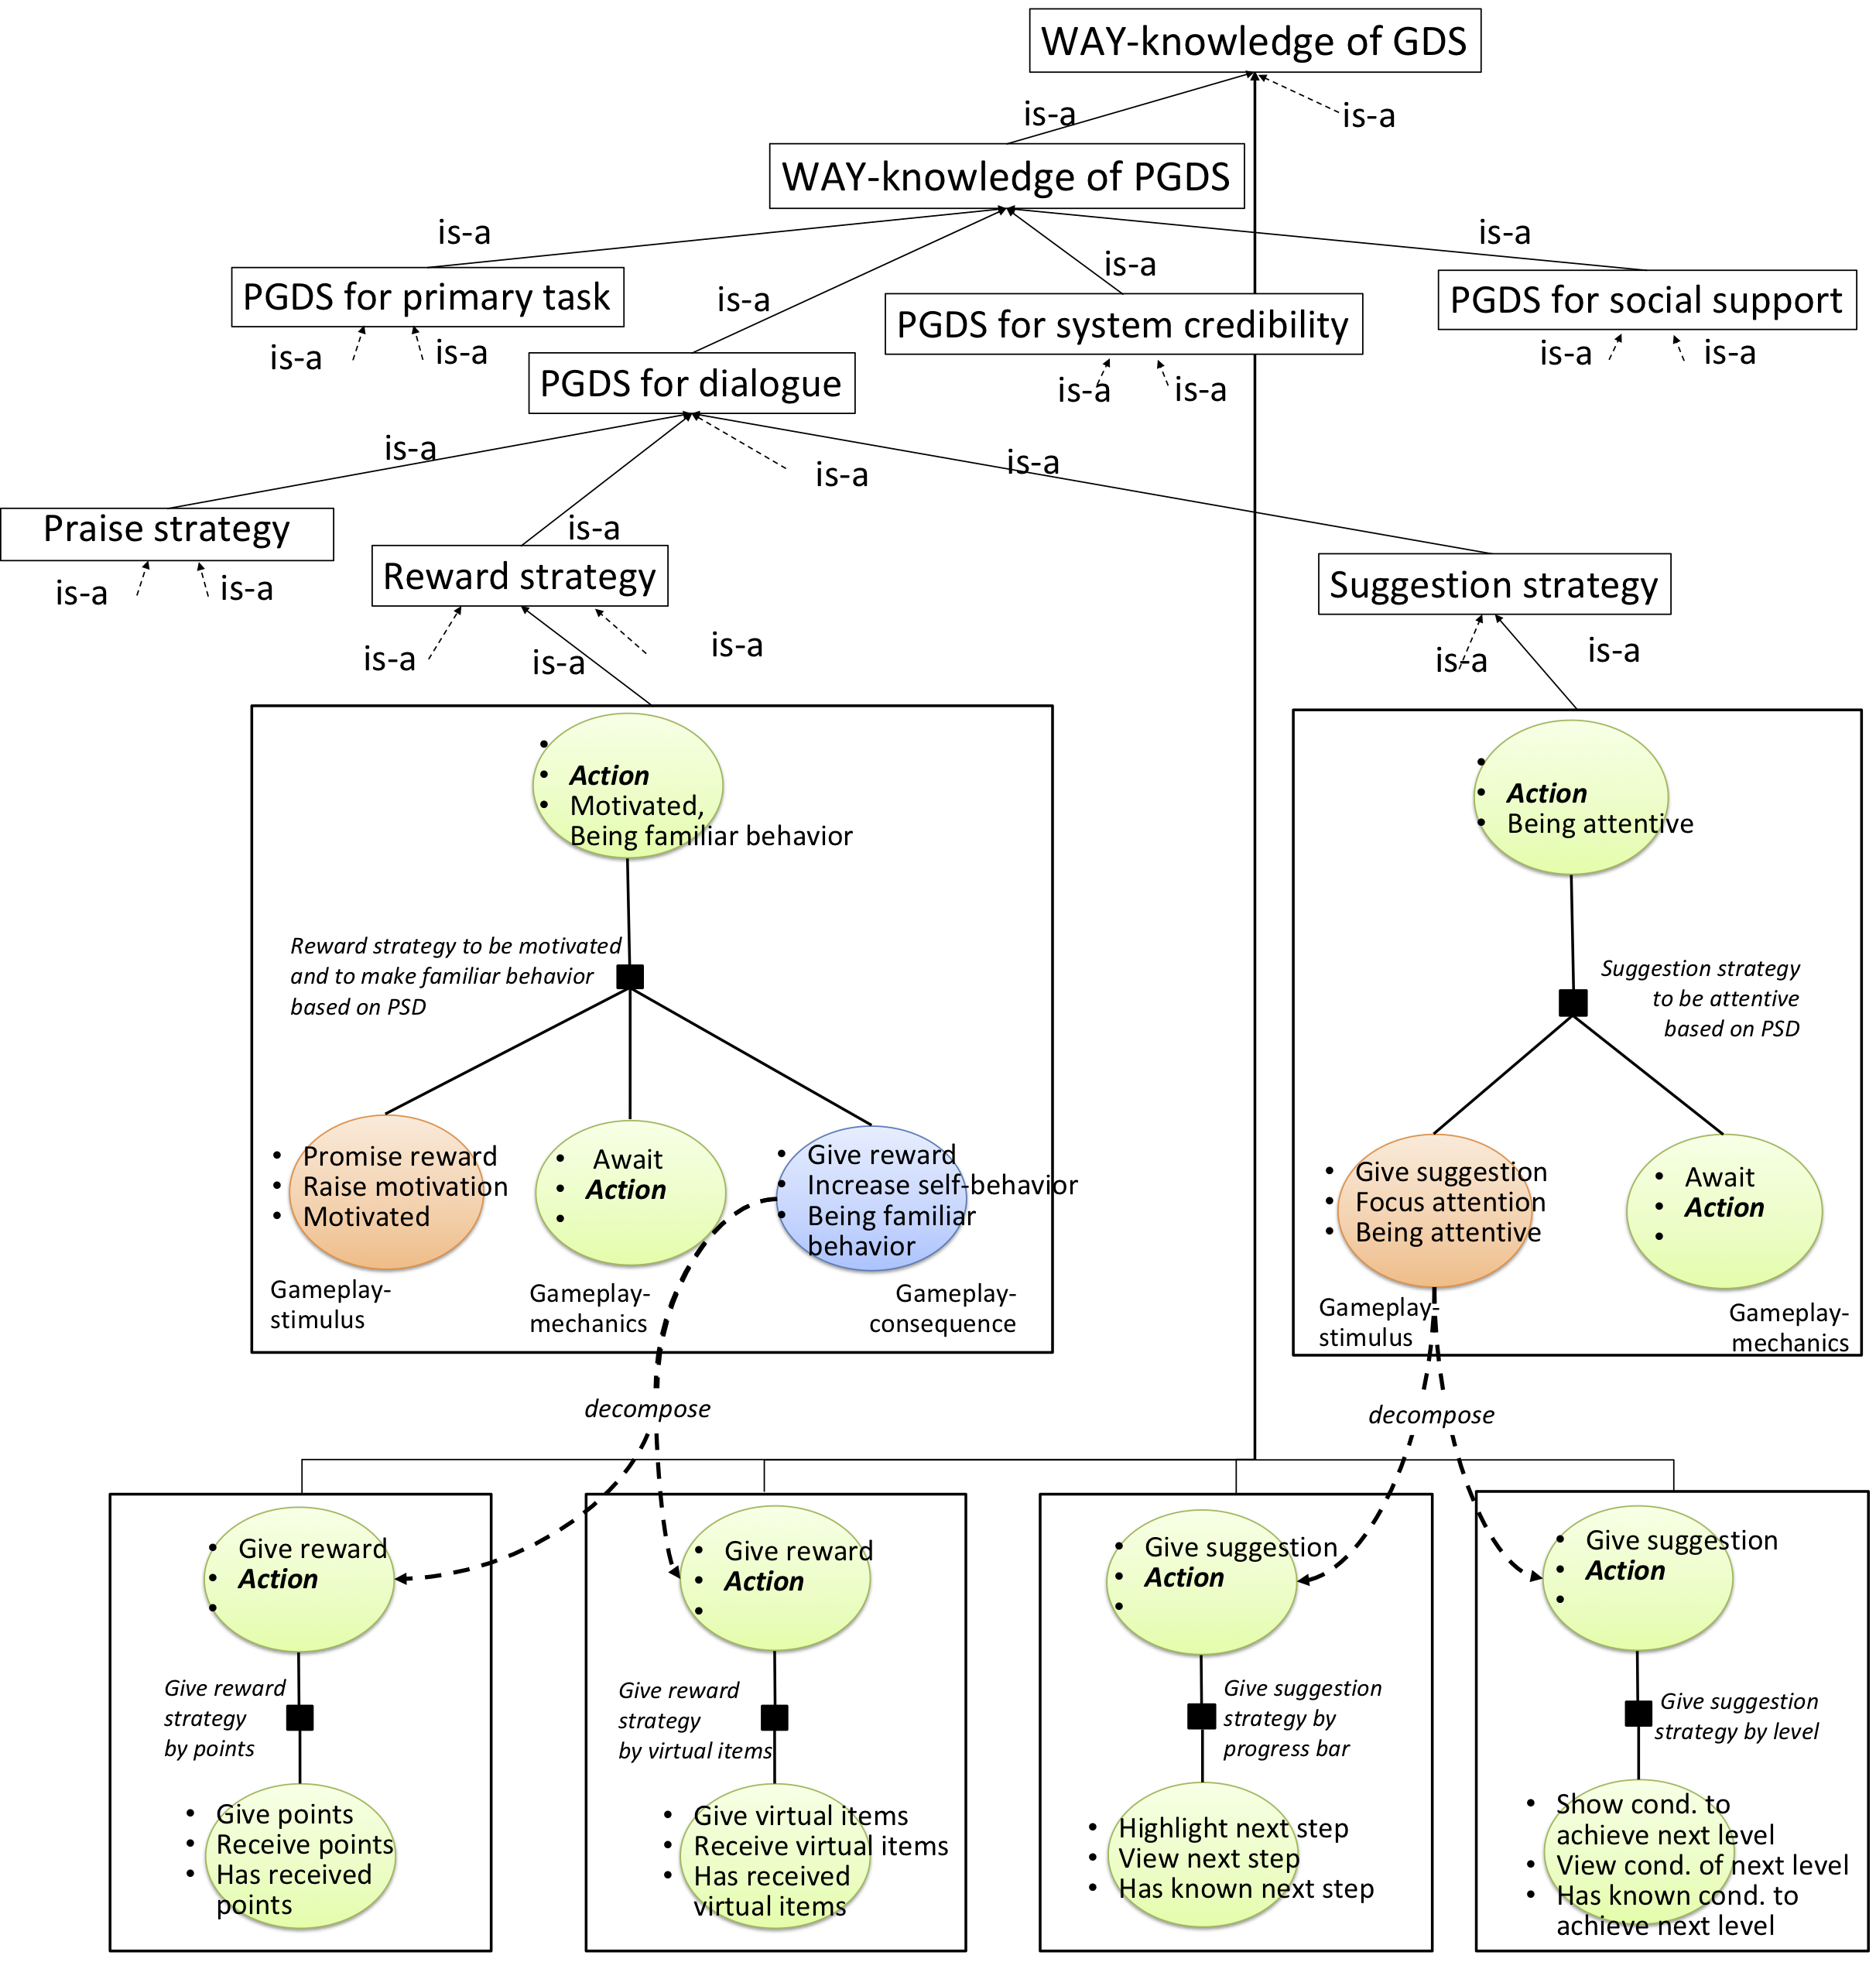
\includegraphics[width=1\textwidth]{images/chap-ontogacles2/portion-way-knowledge-base-pgds.png}
 \fautor
\end{figure}

\autoref{fig:portion-way-knowledge-base-pgds} also shows the decomposition tree of four GDSs that has been formalized based on the information extracted from the Model-driven persuasive game proposed by \citeonline{Orji2014}.
The former two, known as \aspas{\emph{Give reward strategy by points}} and \aspas{\emph{Give reward strategy by virtual items},} are GDSs in which the game actions \aspas{\emph{Give points}} and \aspas{\emph{Give virtual items}} cause the \emph{Terminal state} \aspas{\emph{Has received points}} and \aspas{\emph{Has received virtual items}} by the actions \aspas{\emph{Receive points}} and \aspas{\emph{Receive virtual item}.}
The latter two GDSs are \aspas{\emph{Give suggestion strategy by progress bar}} and \aspas{\emph{Give suggestion strategy by level}} to achieve the \emph{Terminal state}  \aspas{\emph{Has known next step}} and \aspas{\emph{Has known cond. to achieve next level}} by the actions \aspas{\emph{View next step}} and \aspas{\emph{View cond. of next level}.}

The ontological structure to represent the PGDS \aspas{\emph{Reward strategy to be motivated and to make familiar behavior based on PSD}} is shown in \autoref{fig:ontological-structure-reward-strategy-psd}, where the \emph{Terminal state} as goal of the decomposition tree is defined as \emph{Being attentive} in the \emph{macro}-gameplay event.
The sequence of \emph{micro}-gameplay events defined by this PGDS is defined as a gameplay-stimulus event with the game action \aspas{\emph{Give suggestion},} and a gameplay-mechanism event with the game action \aspas{\emph{Await}.}
The terminal state in the gameplay-consequence event is \emph{Being attentive} achieved by the internal psychological process \aspas{\emph{Focus attention}} \emph{influenced by} the game action \aspas{\emph{Give suggestion}.}
This psychological effect has theoretical justification in the ARCS model \cite{Keller1987} indicated in the attribute of \emph{reference} in the \emph{Psychological event} of the \emph{Gameplay-stimulus event}.

\begin{figure}[!htb]
 \caption[Ontological structure to represent the \emph{Suggestion strategy to be attentive based on PSD}]{Ontological structure to represent the \aspas{\emph{Suggestion strategy to be attentive based on PSD}}}
 \label{fig:ontological-structure-reward-strategy-psd}
 \centering
 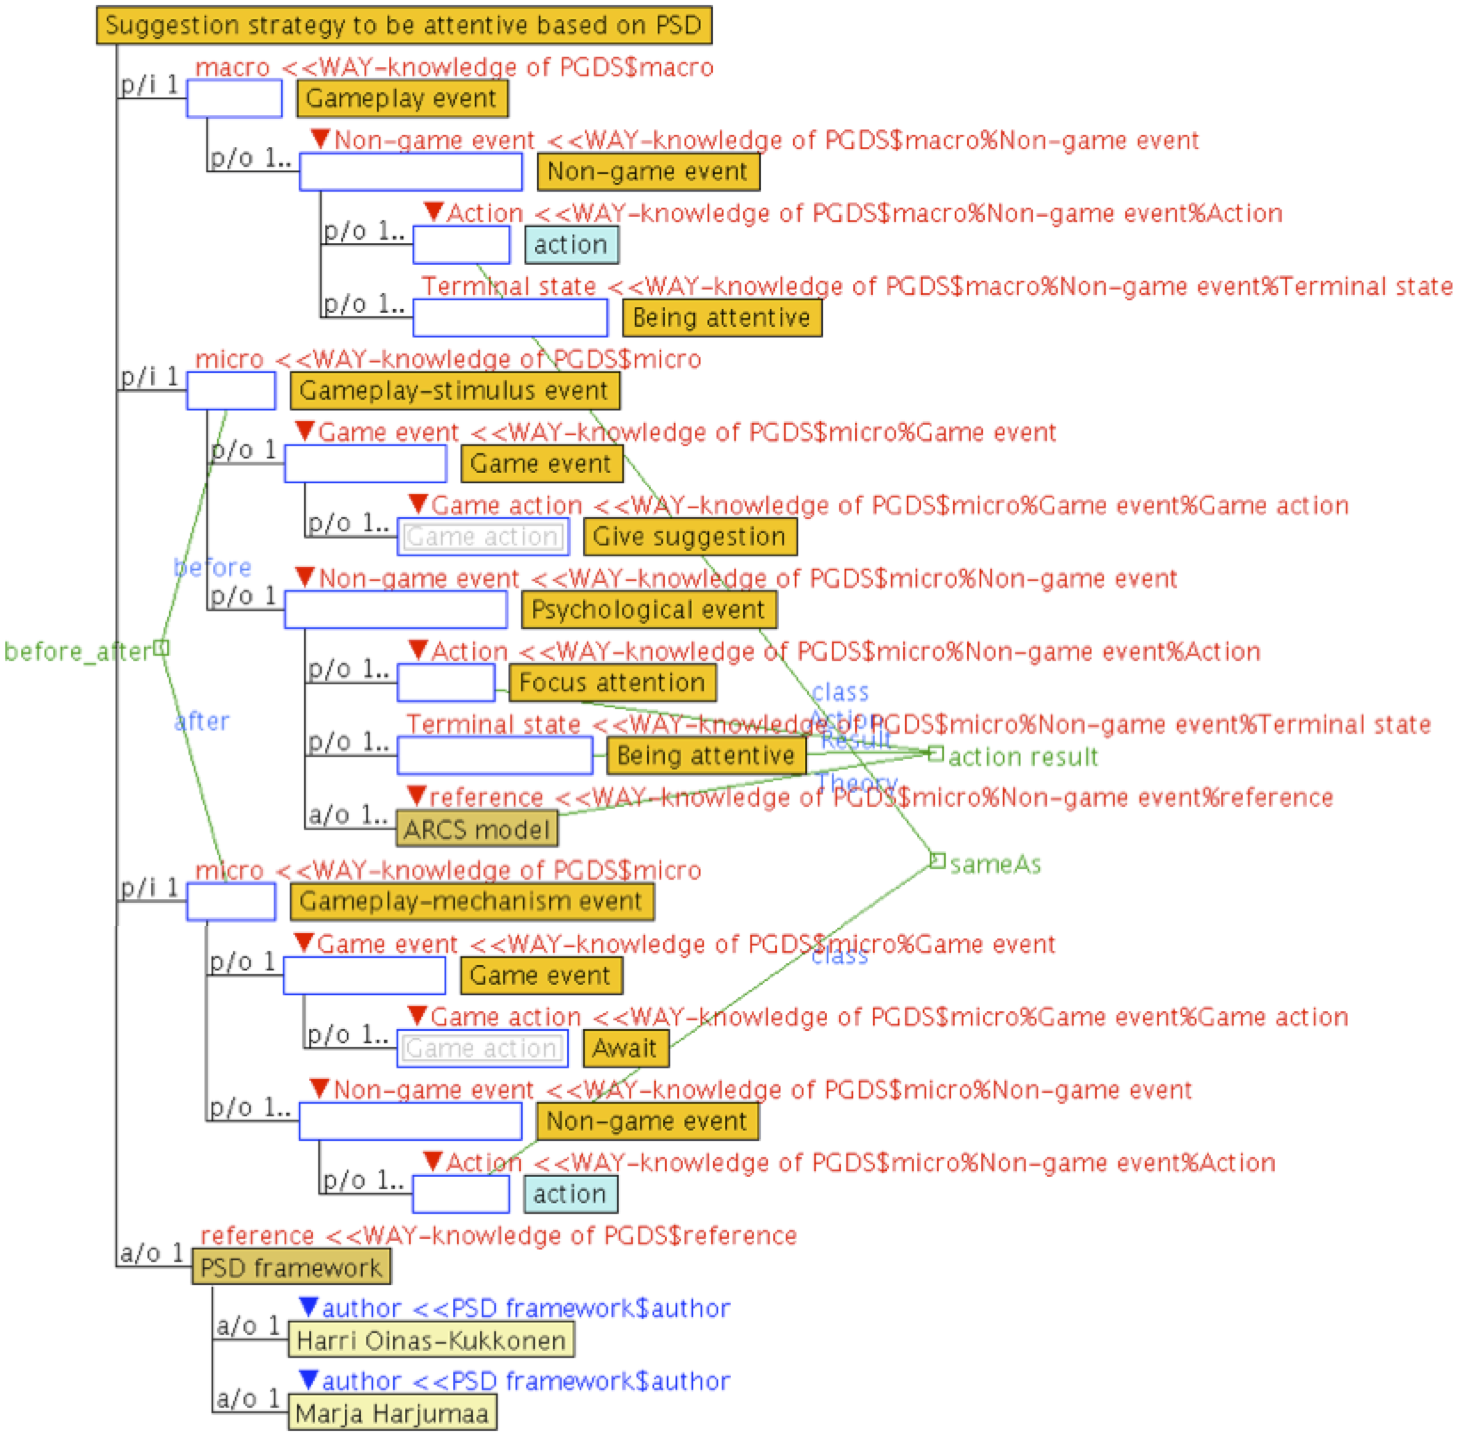
\includegraphics[width=0.9\textwidth]{images/chap-ontogacles2/ontological-structure-reward-strategy-psd.png}
 \fautor
\end{figure}

\subsection{Persuasive Gameplay Scenario Model}
\label{subsec:persuasive-gameplay-scenario-model}

\aspas{\emph{Persuasive Gameplay Scenario Model}} is an abstract structure to indicate the design rationale involved in the application of PGD in non-game events.
This design rationale indicates the changes in the participants' attitudes, intentions, motivations and/or behaviors, and how these changes are achieved by a sequence of gameplay-events.
The persuasive gameplay scenario model is constructed by applying the PGDSs into non-game events in a phased manner obtaining a sequence of gameplay-stimulus, gameplay-mechanisms and game-consequence events.
The determination of when to stop the application of PGDSs is arbitrary for the model authors, and lies outside the scope of the modeling.
\autoref{fig:ontological-structure-persuasive-gameplay-scenario-model} shows the ontological structures proposed in the ontology OntoGaCLeS to represent a persuasive gameplay scenario model.
In the ontological structure \aspas{\emph{Gameplay Scenario Model},} the \emph{WAY-knowledge of GDS} is represented as a link between two gameplay events playing the roles of \emph{root} and \emph{sub} to delineate the \emph{macro}-gameplay event and the sequence of \emph{micro}-gameplay events resulting of the decomposition method.
In the ontological structure \aspas{\emph{Persuasive Gameplay Scenario Model},} the \emph{WAY-knowledge of PGDS} is represented as a link between a \emph{macro}-gameplay event playing the role of \emph{root}, and four \emph{micro}-gameplay events playing the role of \emph{sub}.
In both ontological structures, the concept of \emph{Gameplay Scenario Model} plays the role of \emph{sub} to represent the recursive application of PGDSs and GDSs in the modeling of design rationale to gamify a non-game event.

\begin{figure}[!htb]
 \caption[Ontological structures to represent a persuasive gameplay scenario model]{Ontological structures to represent a \aspas{\emph{Persuasive Gameplay Scenario Model}}}
 \label{fig:ontological-structure-persuasive-gameplay-scenario-model}
 \centering
 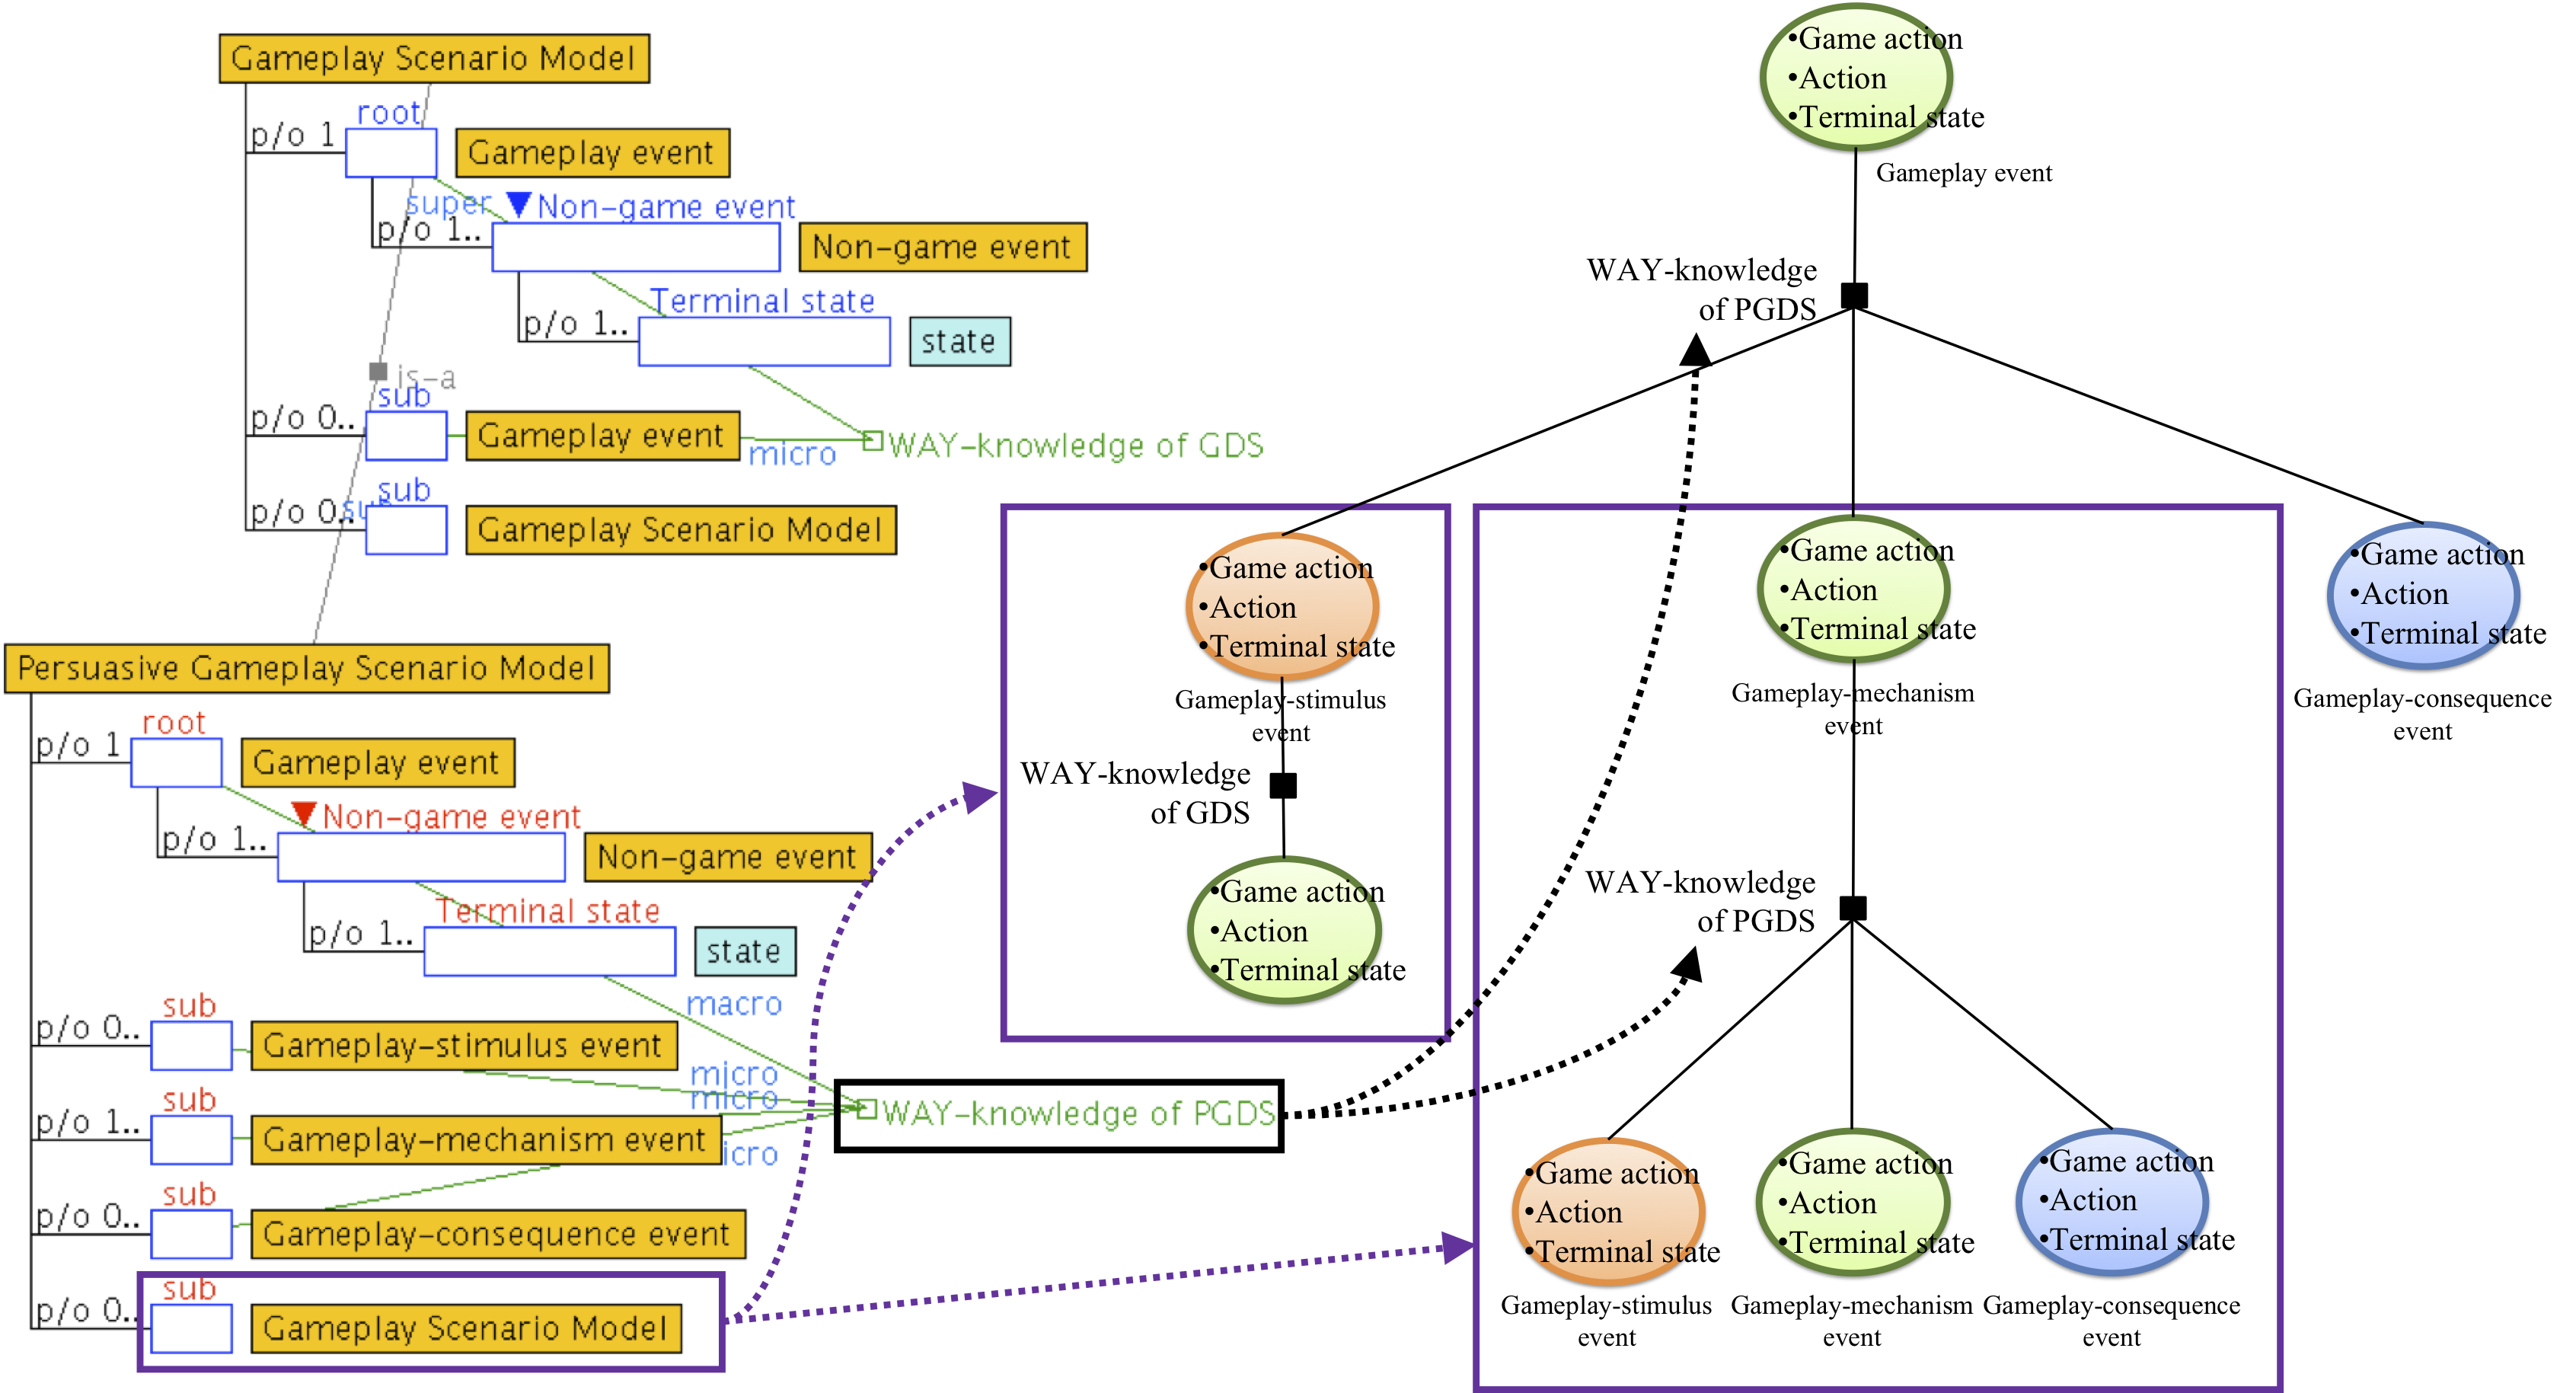
\includegraphics[width=1\textwidth]{images/chap-ontogacles2/ontological-structure-persuasive-gameplay-scenario-model.png}
 \fautor
\end{figure}

Employing the decomposition trees presented in \autoref{fig:ontological-structure-persuasive-gameplay-scenario-model},
An example of persuasive gameplay scenario model is shown in \autoref{fig:decomposition-tree-gamified-giving-information-scenario-model}.
This model represents the design rationale to gamify the instructional event \aspas{\emph{Giving information}} obtained by the application of two PGDSs and three GDSs. The PGDS \aspas{\emph{Reward strategy to be motivated and to make familiar behavior based on PDS}} has been applied to achieve the \emph{Terminal state} of \emph{Motivated} and \emph{Being familiar behavior}, and the PGDS \aspas{\emph{Suggestion strategy to be attentive based on PSD}} has been applied to achieve the \emph{Terminal state} of \emph{Being attentive}. 
The GDSs \aspas{\emph{Promise reward strategy by points},} \aspas{\emph{Give suggestion strategy by level},} and \aspas{\emph{Give reward strategy by points}} have been applied to accomplish the game actions \aspas{\emph{Promise reward},} \aspas{\emph{Give suggestion},} and \aspas{\emph{Give reward}} achieving the terminal states of \aspas{\emph{Has received the promise points},} \aspas{\emph{Has known cond. to achieve next level},} and \aspas{\emph{Has received points}.}

\begin{figure}[!htb]
 \caption{Example of persuasive gameplay scenario model for the gamification of \emph{Giving information}}
 \label{fig:decomposition-tree-gamified-giving-information-scenario-model}
 \centering
 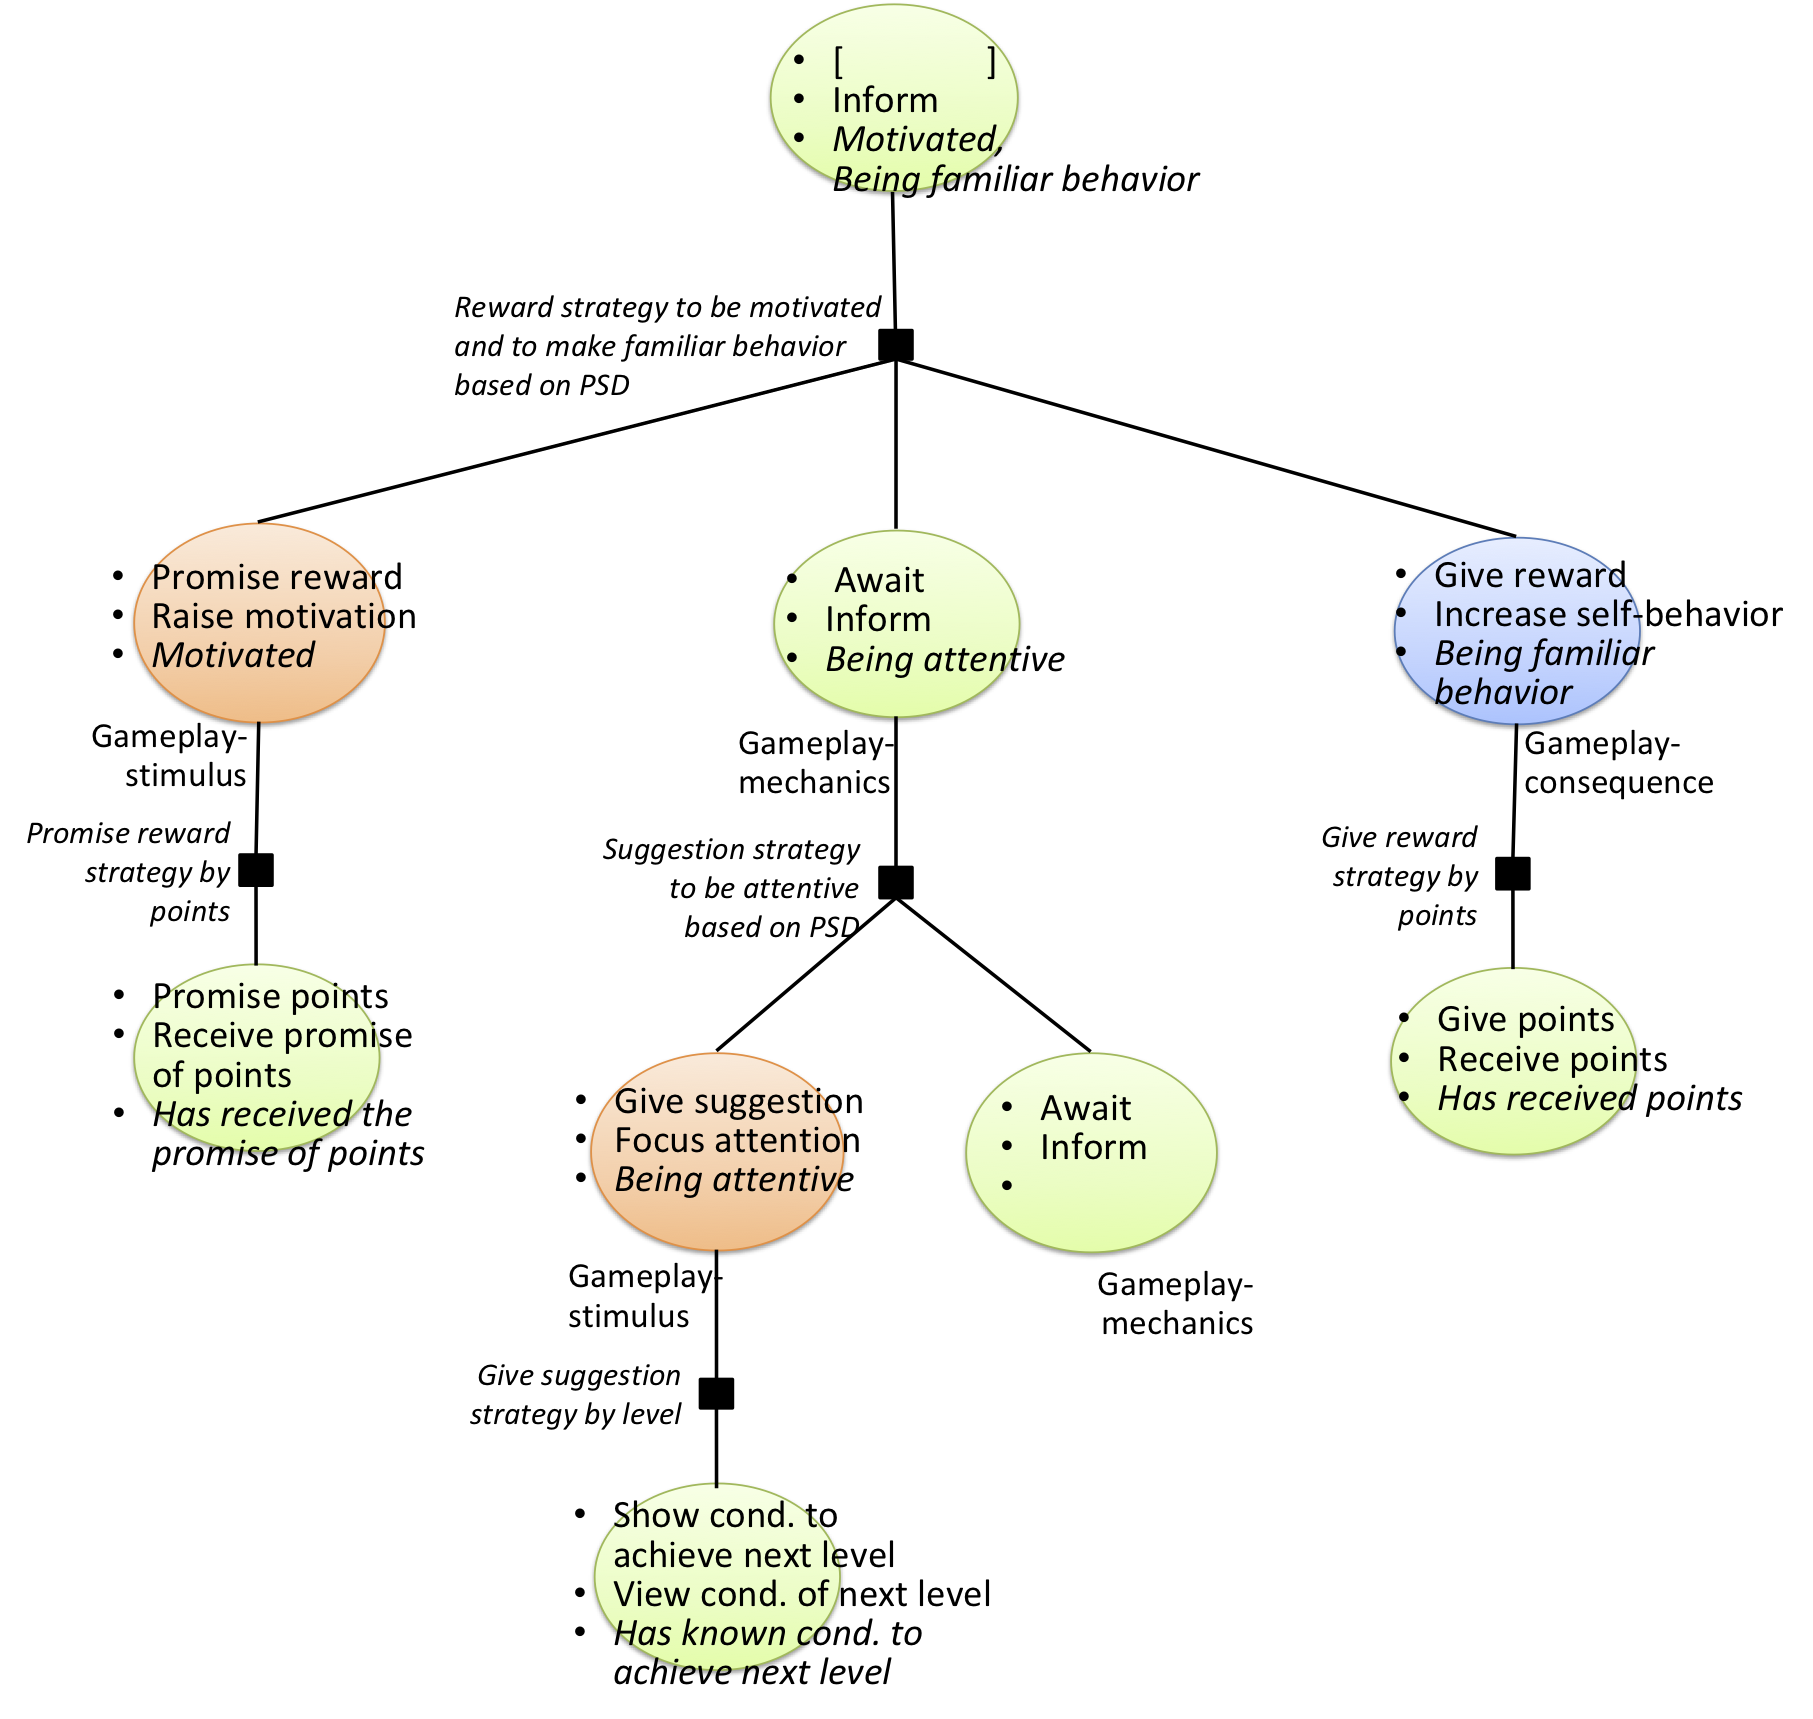
\includegraphics[width=0.85\textwidth]{images/chap-ontogacles2/decomposition-tree-gamified-giving-information-scenario-model.png}
 \fautor
\end{figure}

\autoref{fig:ontological-structure-gamified-giving-information-scenario-model} presents the ontological structure formalized to represent the persuasive gameplay scenario model shown in \autoref{fig:decomposition-tree-gamified-giving-information-scenario-model}. 
According to this structure, the PGDS \aspas{\emph{Reward strategy to be motivated and to make familiar behavior based on PDS}} is represented as a link for a \emph{Gameplay event} and three \emph{micro}-gameplay events defined as a \emph{Gameplay-stimulus event}, a \emph{Gameplay-mechanism event}, and a \emph{Gameplay-consequence event}.
In the \emph{macro}-gameplay event, the goals to be achieved by this PGDS are \aspas{\emph{Motivated}} and \aspas{\emph{Being familiar behavior}} defined as \emph{Terminal state} in the \emph{Non-game event} played by the instructional event \aspas{\emph{Giving information}.}
The GDS \aspas{\emph{Promise reward strategy by points}} is represented as a link between the \emph{macro}- and \emph{micro}-gameplay events defined by the game actions \aspas{\emph{Promise reward}} and \aspas{\emph{Promise points},} respectively.
The \emph{Psychological effect} as terminal state for the action \aspas{\emph{Raise motivation}} in the \emph{Gameplay-stimulus event} defined as \emph{macro}-gameplay event is \emph{Motivated}, and the \emph{Terminal state} for the action \aspas{\emph{Receive promise of points}} defined in the \emph{micro}-gameplay event is \emph{Has received the promise of points}. 
The GDS \aspas{\emph{Give reward strategy by points}} is represented as a link between the \emph{macro}- and \emph{micro}-gameplay events defined by the game actions \aspas{\emph{Give reward}} and \aspas{\emph{Give points},} respectively.
The \emph{Psychological effect} as terminal state for the action \aspas{\emph{Increase self-behavior}} in the \emph{Gameplay-consequence event} defined as \emph{macro}-gameplay event is \emph{Being familiar behavior}, and the \emph{Terminal state} for the action \aspas{\emph{Receive points}} defined in the \emph{micro}-gameplay event is \emph{Has received points}. 
The \emph{Gameplay-mechanism event} defined by the non-game event \aspas{\emph{Giving information}} is decomposed by the PGDS \aspas{\emph{Suggestion strategy to be attentive based on PSD}} into a \emph{Gameplay-stimulus event} and a \emph{Gameplay-mechanism event} to achieve the \emph{Terminal state} of \emph{Being attentive}. 
The \emph{Gameplay-stimulus event} defined by the game action \aspas{\emph{Give suggestion}} causes the \emph{Psychological effect} of \emph{Being attentive} by the psychological process \aspas{\emph{Focus attention}.}
This goal is accomplished by the GDS \aspas{\emph{Give suggestion strategy by level}} in which the game action \aspas{\emph{Show cond. to achieve the next level}} cause the action \aspas{\emph{View cond. of next level}} to achieve the \emph{Terminal state} of \emph{Has known cond. to achieve next level}.

\begin{figure}[!htb]
 \caption{Example of ontological structure to represent the gamification of \emph{Giving information}}
 \label{fig:ontological-structure-gamified-giving-information-scenario-model}
 \centering
 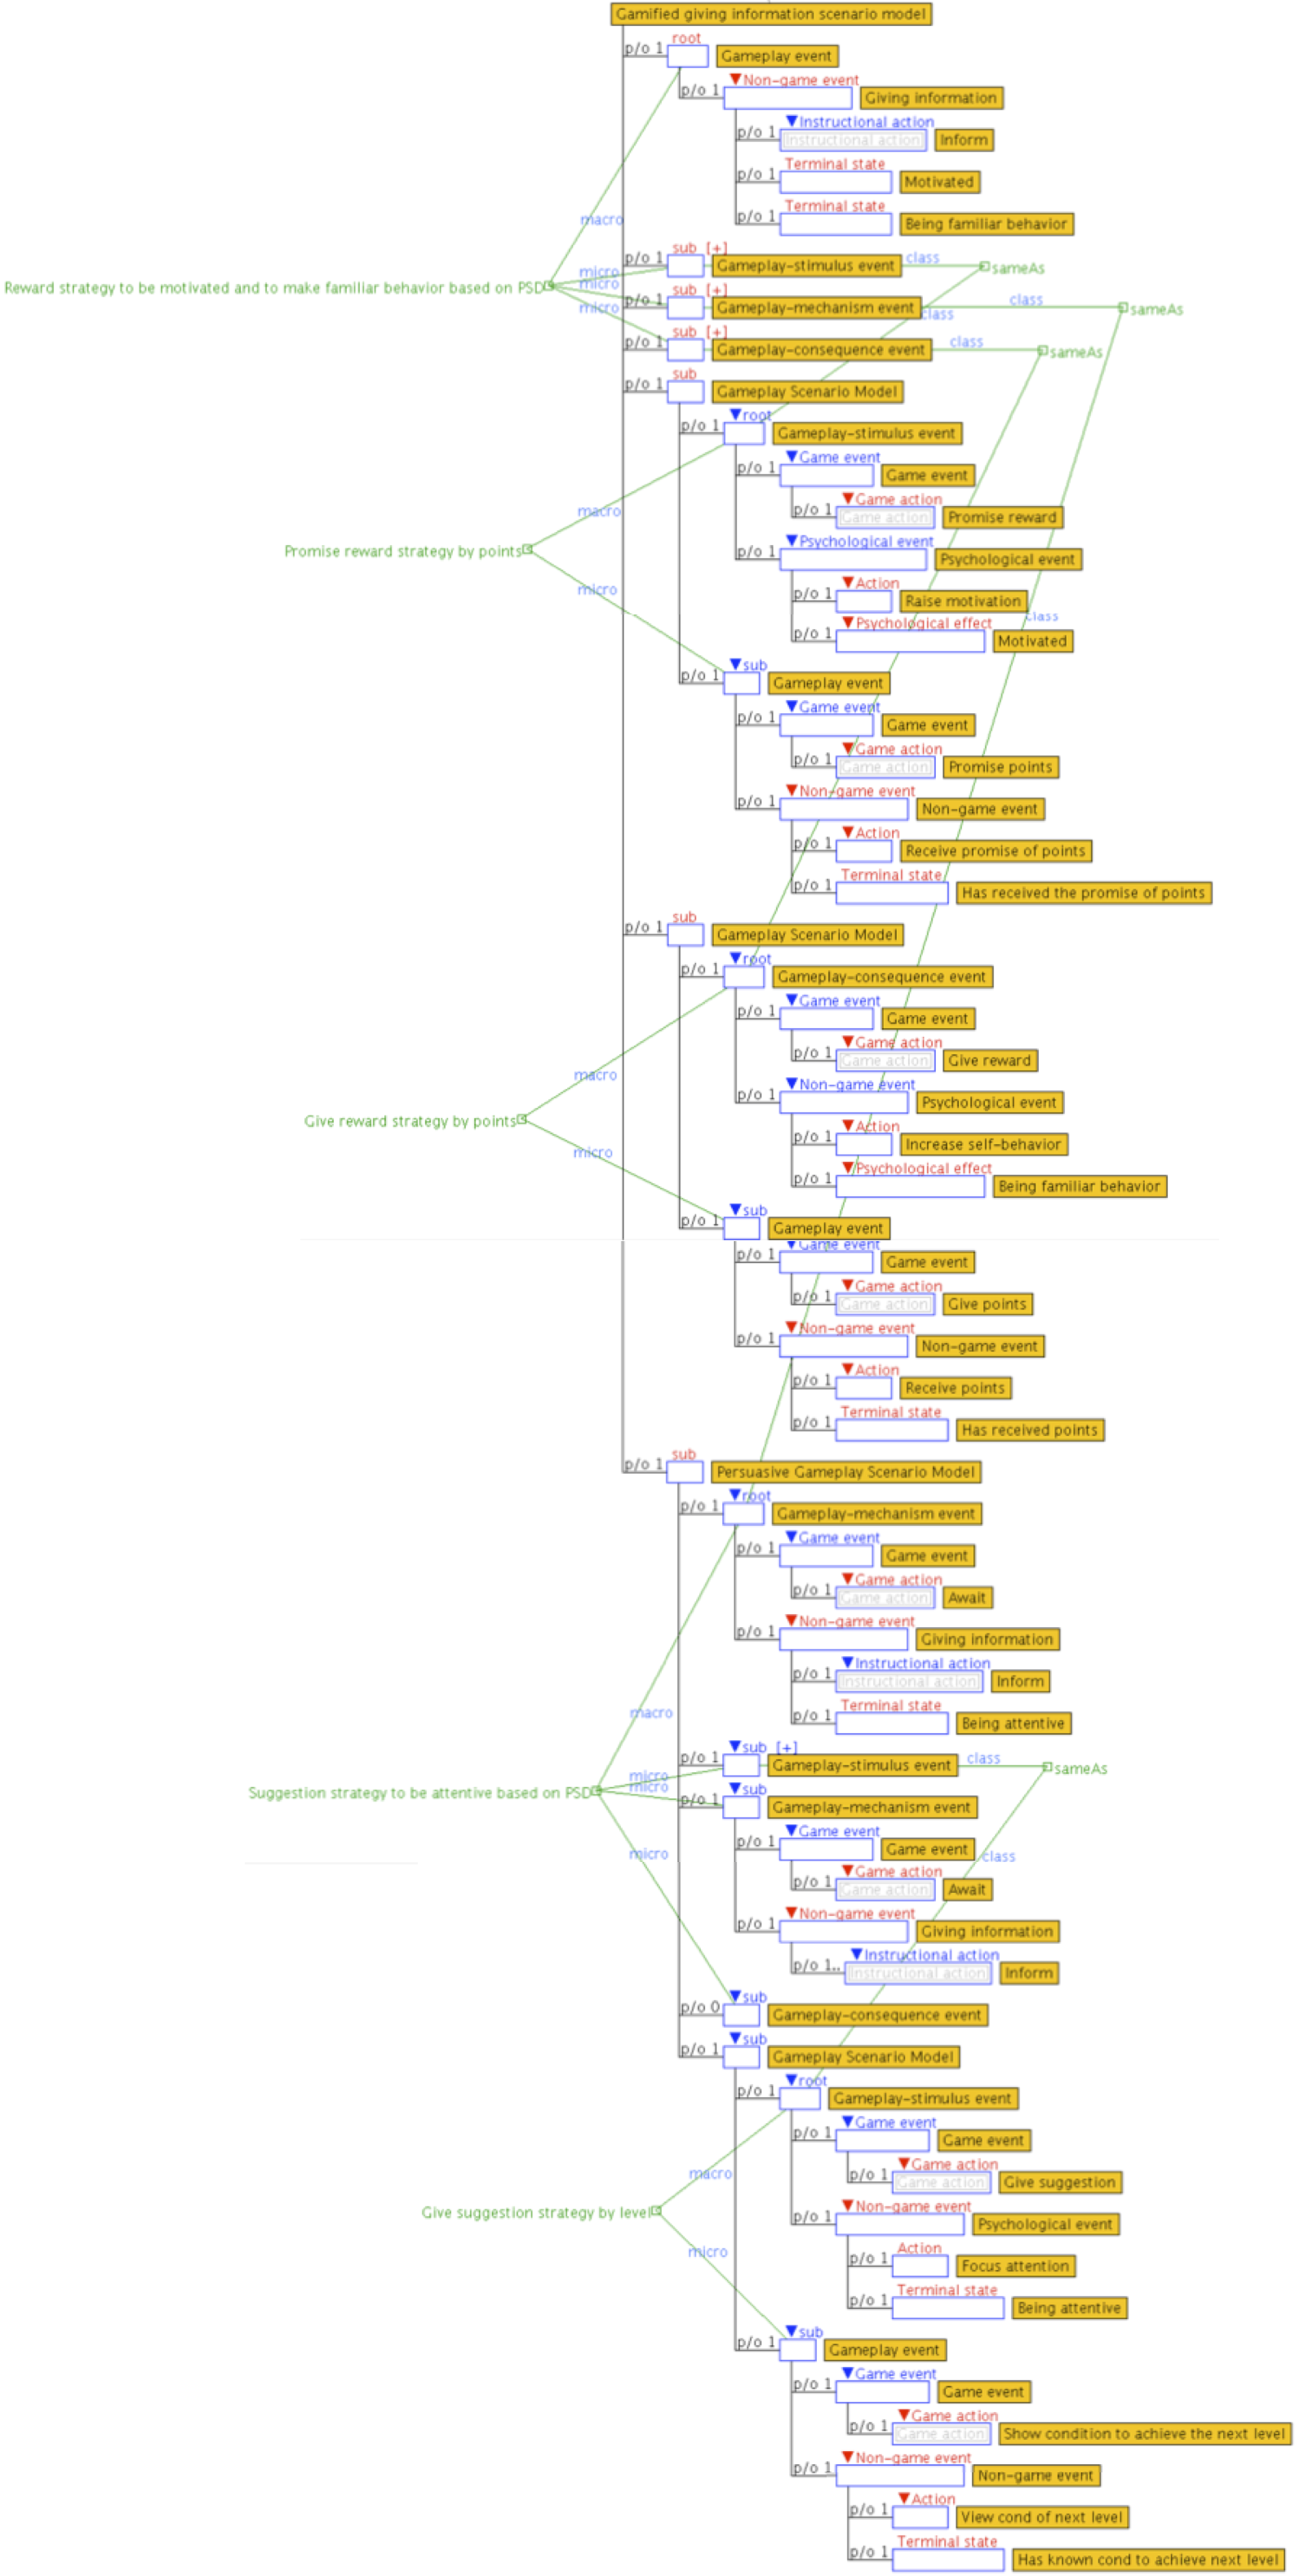
\includegraphics[width=0.7\textwidth]{images/chap-ontogacles2/ontological-structure-gamified-giving-information-scenario-model.png}
 \fautor
\end{figure}
\newpage

%%%%%%%%%%%%%%%%%%%%%%%%%%%%%%%%%%%%%%%%%%%%%%%%%%
\section[Modeling of CL Gameplay Based on Persuasive Game Design]{Modeling of Collaborative Learning Gameplay Based on Persuasive Game Design}
\label{sec:modeling-cl-gameplay-persuasive-game-design}

Having the ontological structures to represent Persuasive Game Design Strategies (PGDSs) and the rational design about how to successively apply them, we can procedure to link the design of CL process and the PGD for dealing with motivational problems in scripted collaborative learning. 
This link was established by the modeling of CL gameplay based on PGD.
The concepts, terms and relations defined in this modeling are shown in \autoref{fig:concepts-terms-and-relation-in-cl-gameplay}, where:

\begin{description}
\item[Gamified I\_L event]
represents the influential I\_L event in which a set of PGDSs has been applied to persuade the participants who play the instructor and learner roles to interact between them performing the instructional and learning actions defined in an I\_L event.

\item[CL Game Dynamic]
describes the run-time behavior of game elements acting to persuade the participants to follow the interactions defined by the sequencing mechanism of a CSCL script. This behavior is defined by the PGDSs applied to interaction patterns.
 
\item[CL Gameplay]
is the set of CL Game dynamics defined in a gamified CL scenario to delineate the whole CL process in a gamified CL scenario.
\end{description}


\begin{figure}[!htbp]
 \caption{Concepts, terms and relations in the modeling of CL gameplay based on PGD}
 \label{fig:concepts-terms-and-relation-in-cl-gameplay}
 \centering
 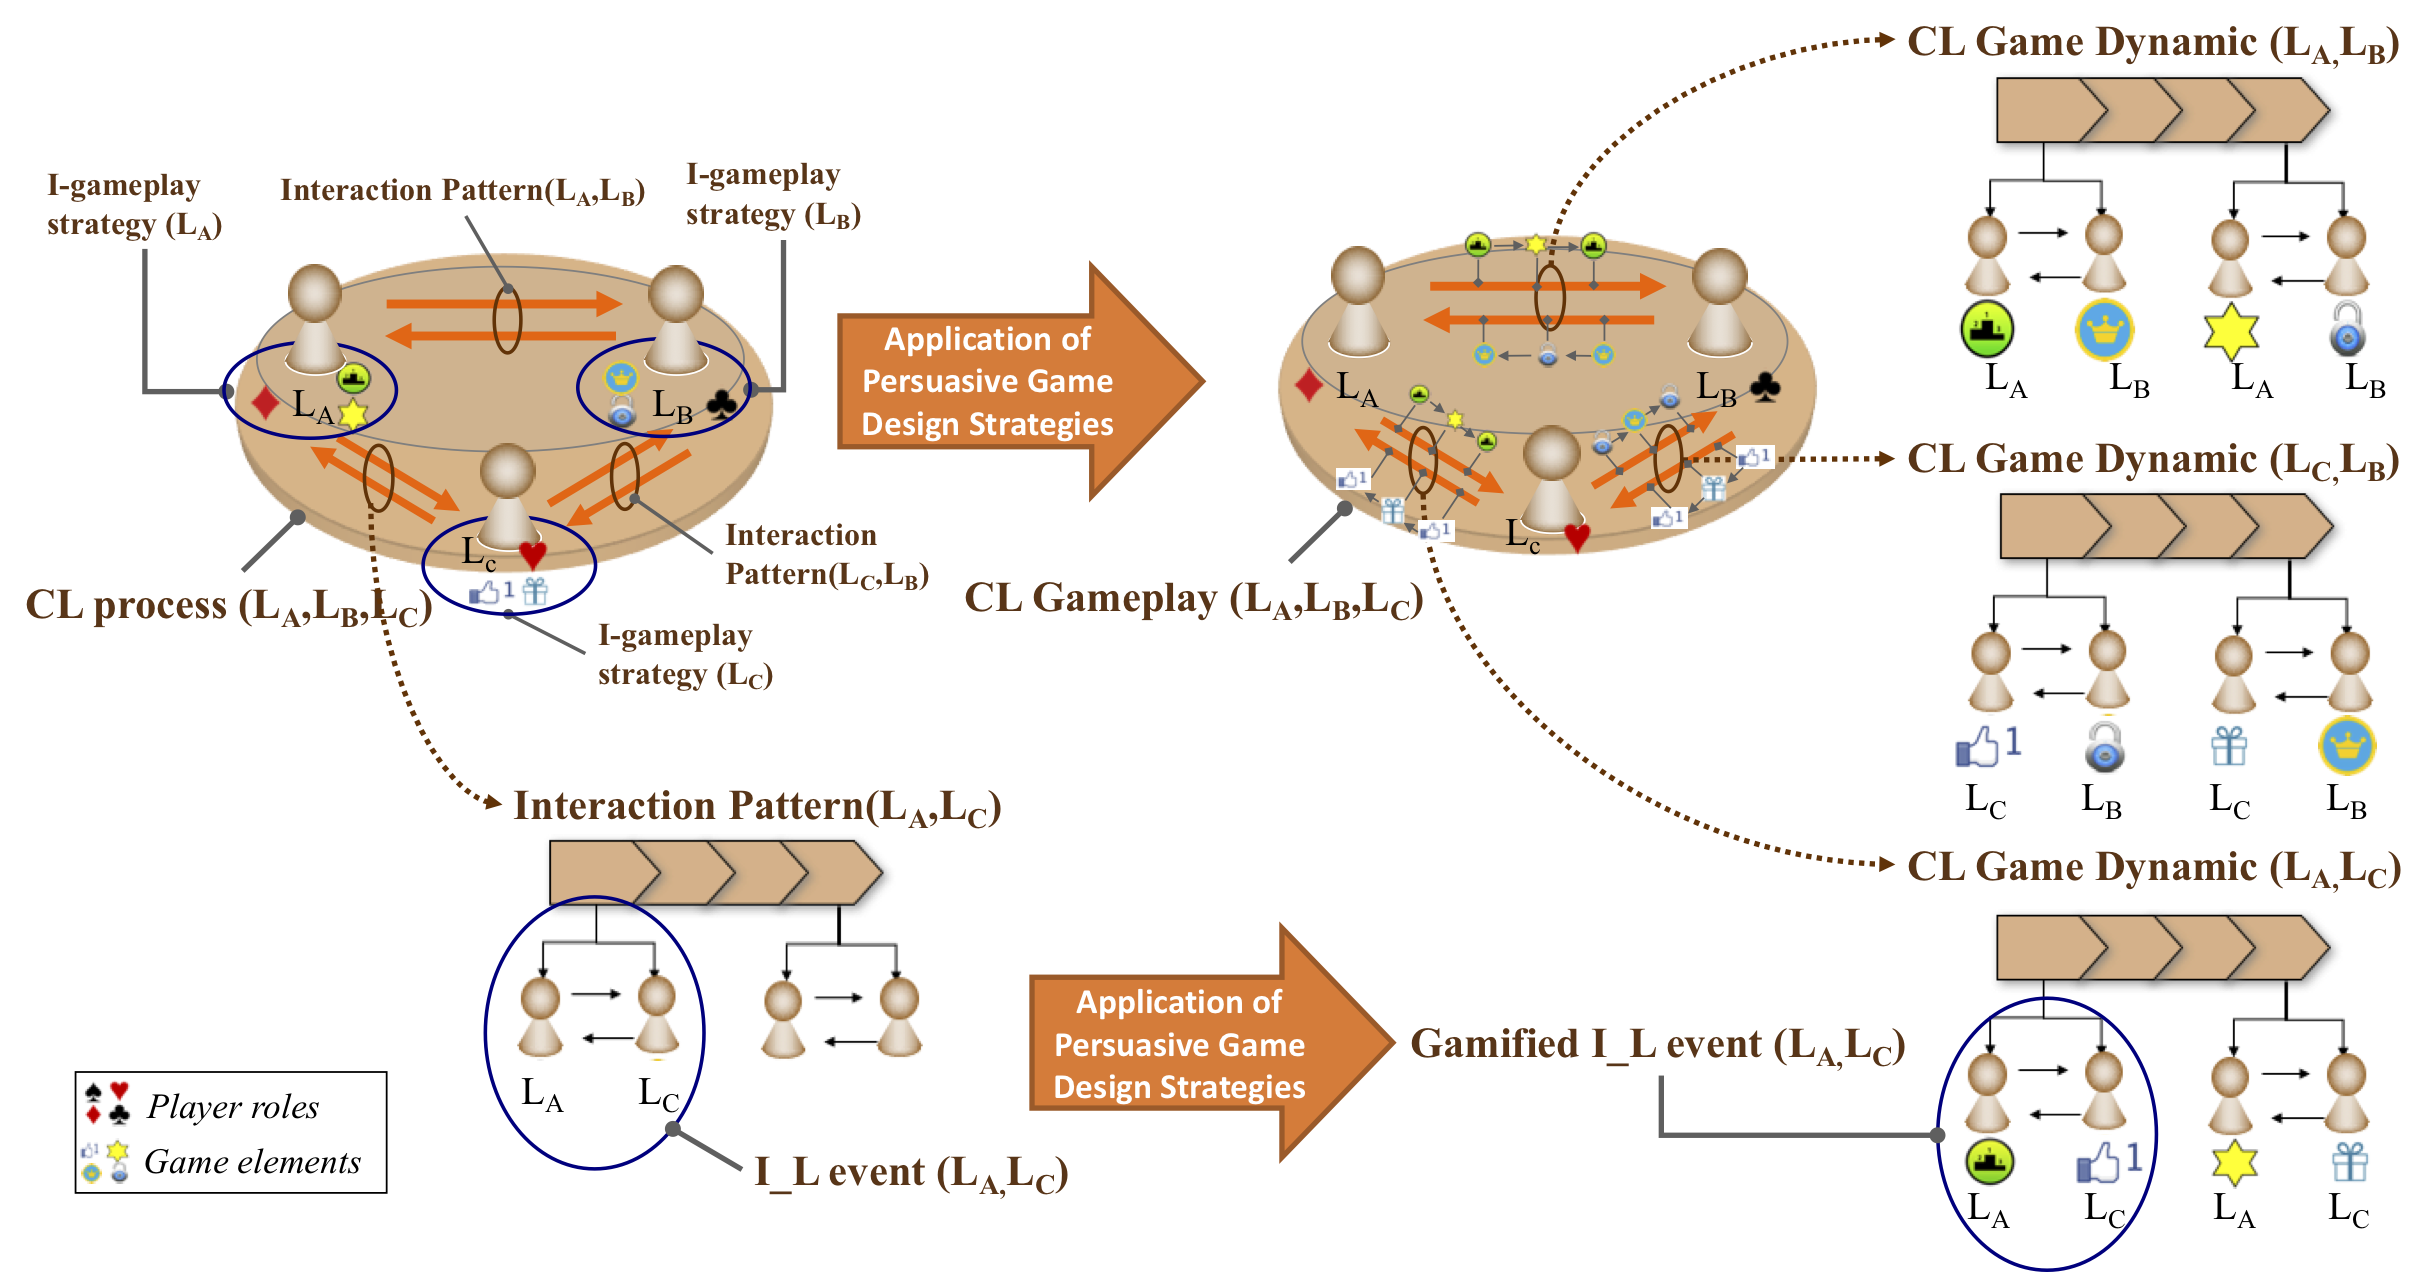
\includegraphics[width=1\textwidth]{images/chap-ontogacles2/concepts-terms-and-relation-in-cl-gameplay.png}
 \fautor
\end{figure}

In the following subsections, the formalization of concepts, terms and relations briefly introduced here are detailed.

\subsection{Gamified I\_L Event}
\label{subsec:gamified-il-event}

In the ontology OntoGaCLeS, the interaction defined by the sequencing mechanism of a CSCL script is represented by two parts: an \emph{Instructional event}, and a \emph{Learning event}.
Thus, in a gamified CL scenario, as shown in \autoref{fig:gameplay-scenario-models-gamified-il-event}, the \emph{Gamified I\_L event} has been formalized an interaction composed by the pairs of events: \emph{Gamified instructional event}, and \emph{Gamified learning event}. 
These both events are the result of applying PGDSs in the instructional and learning events as illustrated in the figure in which the \emph{Gameplay Scenario Model 1} corresponds to the instructional event, and the \emph{Gameplay Scenario Model 2} corresponds to the learning event.

\begin{figure}[!htbp]
 \caption{Elements in a gamified I\_L event}
 \label{fig:gameplay-scenario-models-gamified-il-event}
 \centering
 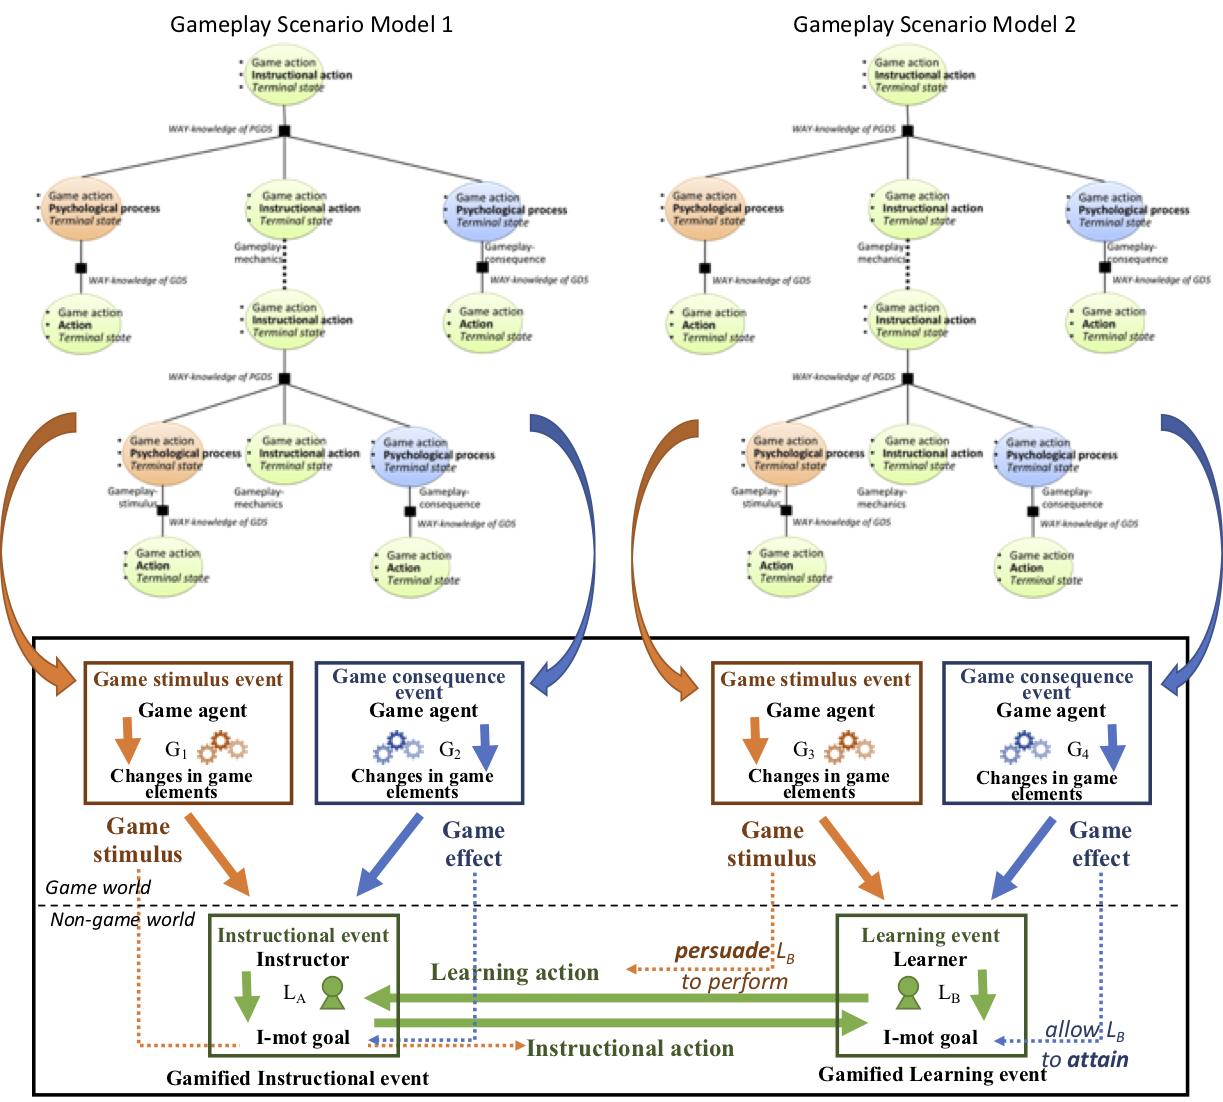
\includegraphics[width=1\textwidth]{images/chap-ontogacles2/gameplay-scenario-models-gamified-il-event.png}
 \fautor
\end{figure}

The gameplay scenarios in a gamified I\_L event delineate the design rationales whereby the instructional and learning events are gamified to influence the instructor and learner role holders to perform the action indicated by the sequencing mechanism of CSCL script.
Such influence is caused by game actions that occur before and after the instructional and learning actions defined in the instructional and learning events.
As shown in \autoref{fig:gameplay-scenario-models-gamified-il-event}, when these game actions are derived from gameplay-stimulus events occurring before the instructional and learning actions, they become \emph{game stimulus}; and when these game actions are derived from gameplay-consequence events occurring after the instructional and learning actions, they become \emph{game effects}.
The game stimulus, the game agents ($G_{1}$ and $G_{3}$) performing these stimuli, and the changes in game elements caused by the game stimulus are formalized as game stimulus events.
The game effects, the game agents ($G_{2}$ and $G_{4}$) performing these effects, and the changes in game elements caused by the game effects are formalized as game consequence events.
In this sense, the game actions as game stimulus carried out by the game agents ($G_{1}$ and $G_{3}$) \emph{persuade} the instructor ($L_{A}$) and learner ($L_{B}$) to perform the instructional and learning actions indicated in the instructional and learning events.
The game actions carried out by the game agents ($G_{2}$ and $G_{4}$) are game effects that allow to the instructor ($L_{A}$) and ($L_{B}$) to \emph{attain} individual motivational goals (\emph{I-mot goal}).
These individual motivational goals represent the contemplated changes in the motivational stage of participants ($L_{A}$ and $L_{B}$) to interact between them.

The ontological structure proposed in the ontology OntoGaCLeS to represent a \aspas{\emph{Gamified I\_L event}} is shown at the top of \autoref{fig:ontological-structure-gamified-il-event}.
According to this structure, the role of \emph{Gamified I event} is played by a \emph{Gamified instructional event}, and the role of \emph{Gamified L event} is played by a \emph{Gamified learning event}.
The \emph{Gamified instructional event} is composed by: a \emph{Game stimulus event} played by a \emph{Game event}, a \emph{Game consequence event} played by a \emph{Game event}, and a \emph{Game mechanism event} played by an \emph{Instructional event}.
The \emph{Gamified learning event} is composed by: a \emph{Game stimulus event} played by a \emph{Game event}, a \emph{Game consequence event} played by a \emph{Game event}, and a \emph{Game mechanism event} played by a \emph{Learning event}.
The instructional and learning events become game mechanism events because, when these events are gamified by the application of PGDSs, the instructional and learning actions are game mechanisms invoked by the instructor and learner to push forward through the game elements, and thus, to \emph{attain} individual motivational goals (\emph{I-mot goal}).
These individual motivational goals are represented in the ontological structure as \emph{Benefits for the player} that can be achieved by the instructor and learner by performing the actions indicated in the instructional and learning events.
The link \aspas{\emph{persuade}} in the \emph{Gamified I event} and \emph{Gamified L event} indicates the relation concept between game stimulus and instructional/learning actions.
This link represents the instructional and learning actions influenced by persuasion and/or social influence.
The link \aspas{\emph{attain}} in these both gamified events (\emph{Gamified I event} and \emph{Gamified L event}) indicates the relation concept between game effects and individual motivational goals (\emph{I-mot goal}) in which the game effects are actions that allow the learner and instructor to accomplish the individual motivation goals.

\begin{figure}[!htbp]
 \caption[Ontological structure to represent a \emph{Gamified I\_L event}]{Ontological structure to represent a \aspas{\emph{Gamified I\_L event}} (at the top). At the bottom, an example of Gamified I\_L event \aspas{\emph{Gamified Notify how the learner is}} as ontological structure.}
 \label{fig:ontological-structure-gamified-il-event}
 \centering
 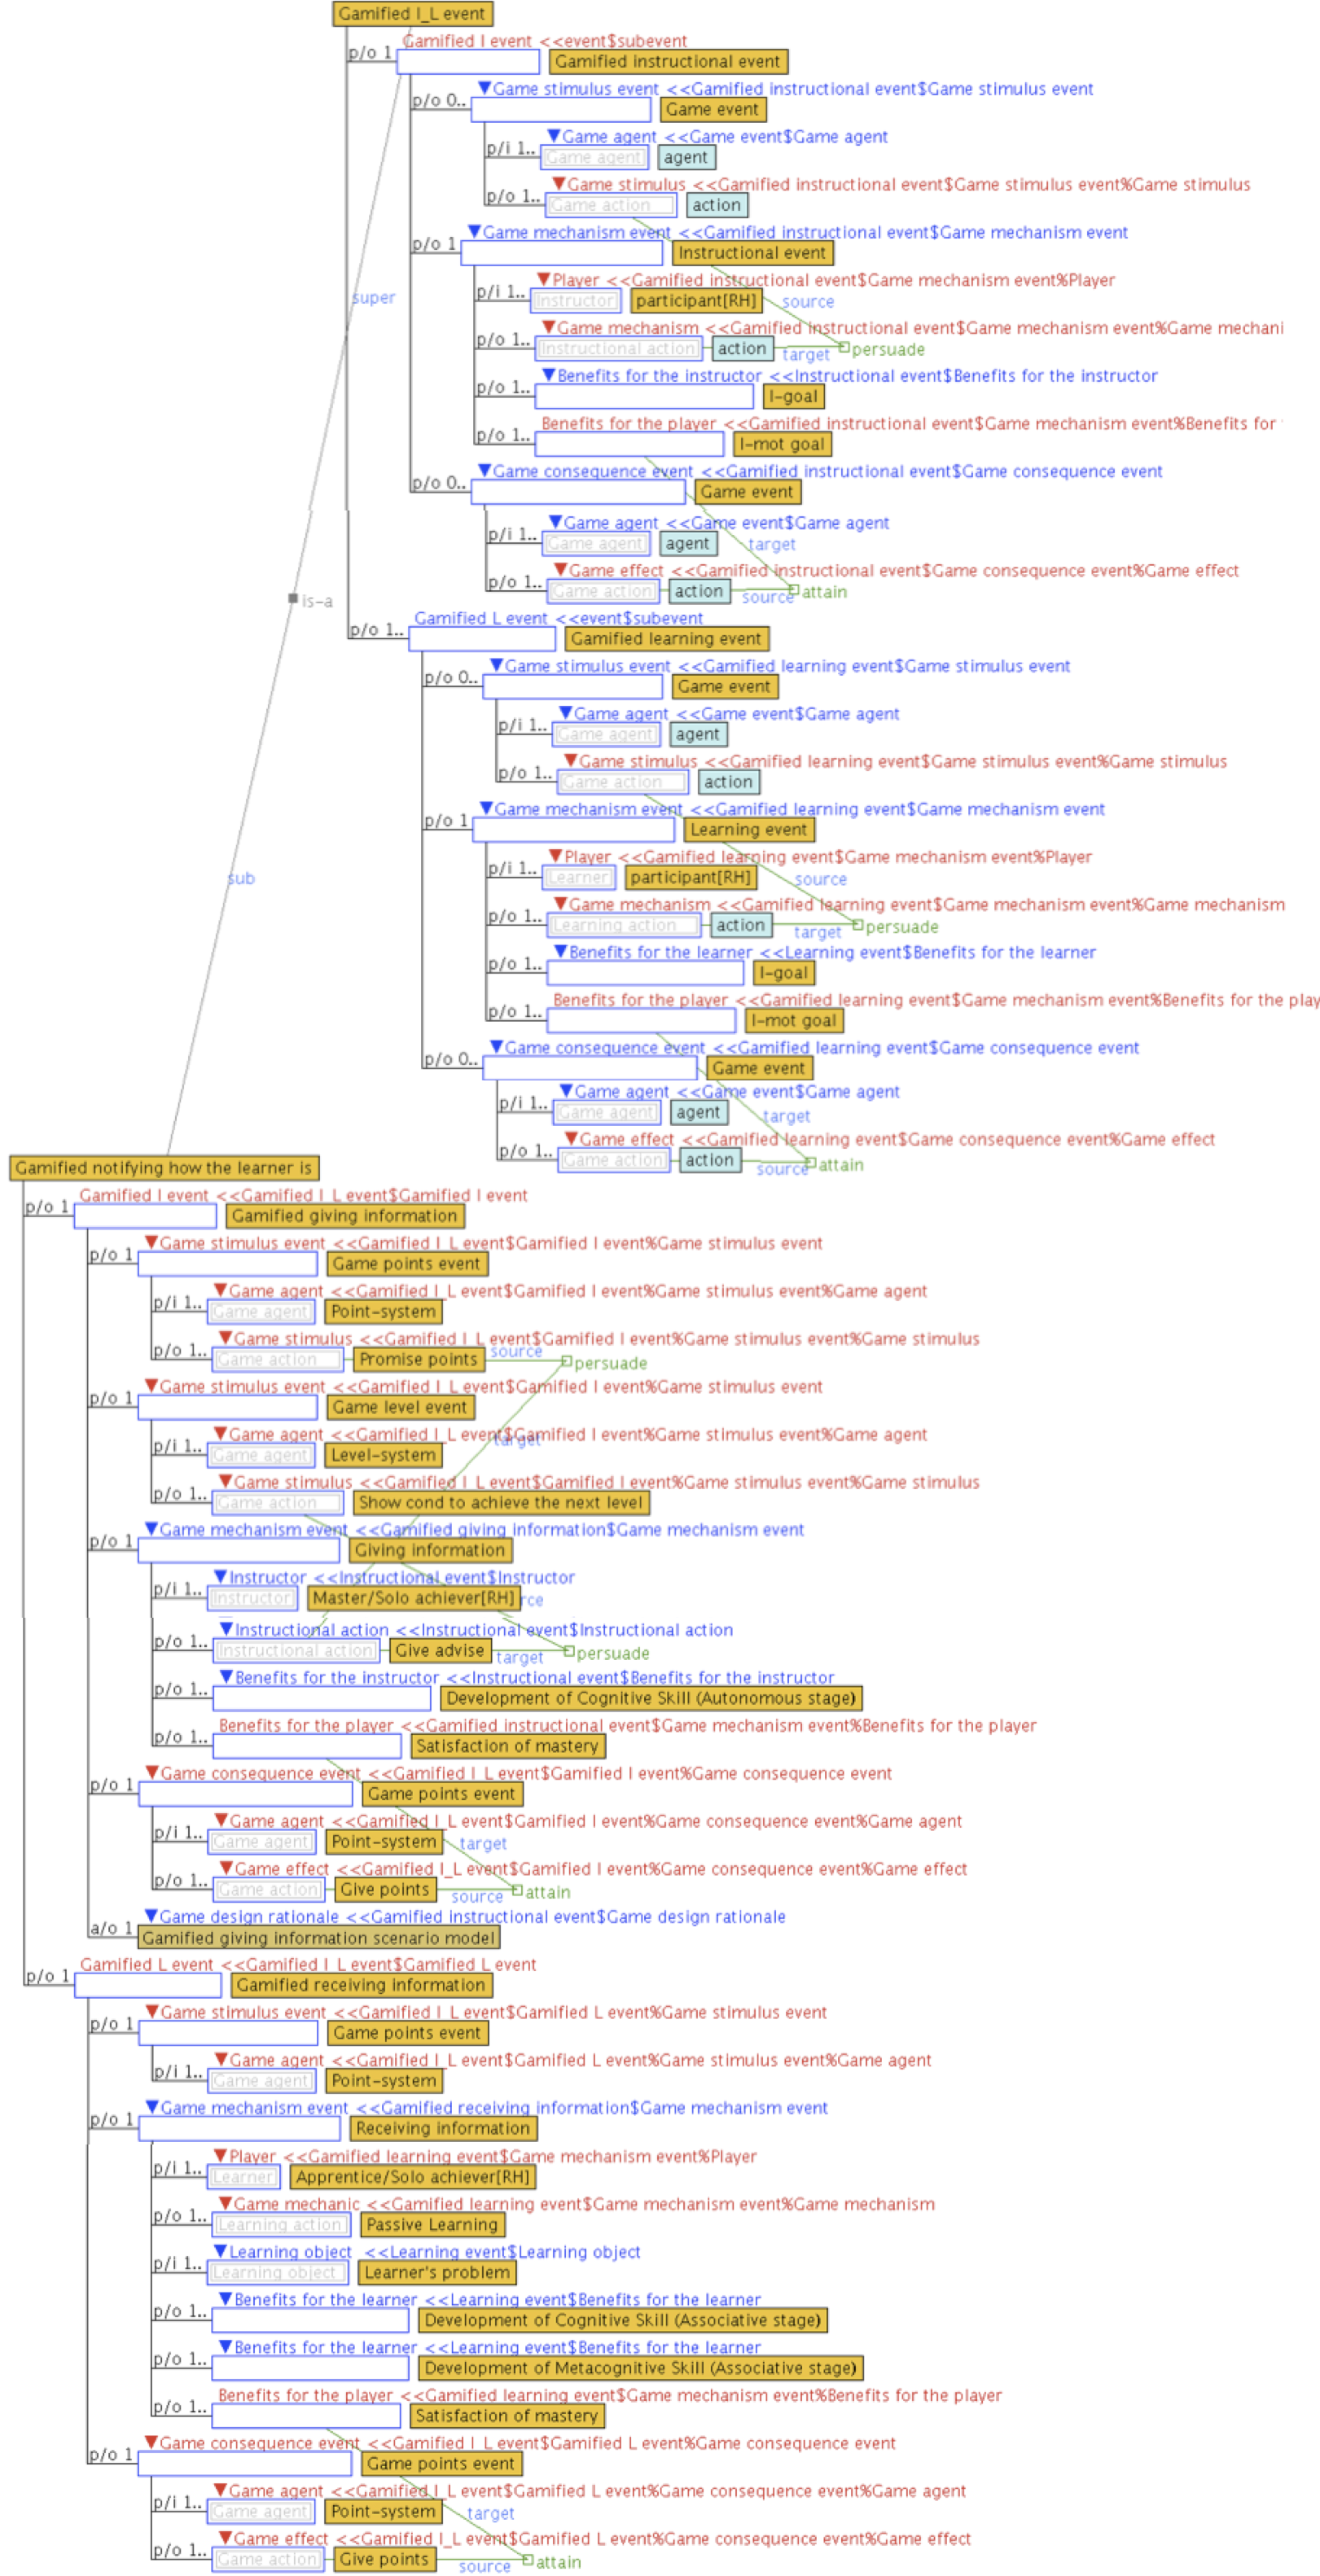
\includegraphics[width=0.74\textwidth]{images/chap-ontogacles2/ontological-structure-gamified-il-event.png}
 \fautor
\end{figure}
\newpage

At the bottom of \autoref{fig:ontological-structure-gamified-il-event}, there is shown the ontological structure to represent a Gamified I\_L event \aspas{\emph{Gamified Notify how the learner is}} illustrated in \autoref{fig:elements-gamified-notify-how-learner-is}.
This ontological structure is the result of applying the PGDSs and GDSs of \emph{Gameplay Scenario Model 1} and \emph{Gameplay Scenario Model 2} for the Instructional event \aspas{\emph{Giving information}} and the Learning event \aspas{\emph{Receiving information}.}
The \emph{Gameplay Scenario Model 1} is indicated as the attribute \aspas{\emph{Game design rationale}} in the \emph{Gamified giving information}. 
According to this game design rationale, a game points event becomes game stimulus event when the game action \aspas{\emph{Promise points}} as game stimulus carried out by the \emph{Point-system} persuades the \emph{Master/Solo achiever role holder} as instructor to perform the instructional action \aspas{\emph{Give advise}} that becomes game mechanism.
A game level event becomes game stimulus event when the game action \aspas{\emph{Show cond. to achieve the next level}} as game stimulus carried out by the \emph{Level-system} persuades the \emph{Master/Solo achiever role holder} as instructor to perform the instructional action \aspas{\emph{Give advise}} that becomes game mechanism.
The game points event becomes game consequence event when the game action \aspas{\emph{Give points}} performed by the \emph{Point-system} allows the \emph{Master/Solo achiever role holder} as instructor to \emph{attain} the \emph{Satisfaction of mastery} defined as \emph{Benefits for the player}.

\begin{figure}[!htbp]
 \caption[Elements in the example of gamified I\_L event \aspas{\emph{Gamified Notify how the learner is}.}]{Elements in an example of gamified I\_L event \aspas{\emph{Gamified Notify how the learner is}.}}
 \label{fig:elements-gamified-notify-how-learner-is}
 \centering
 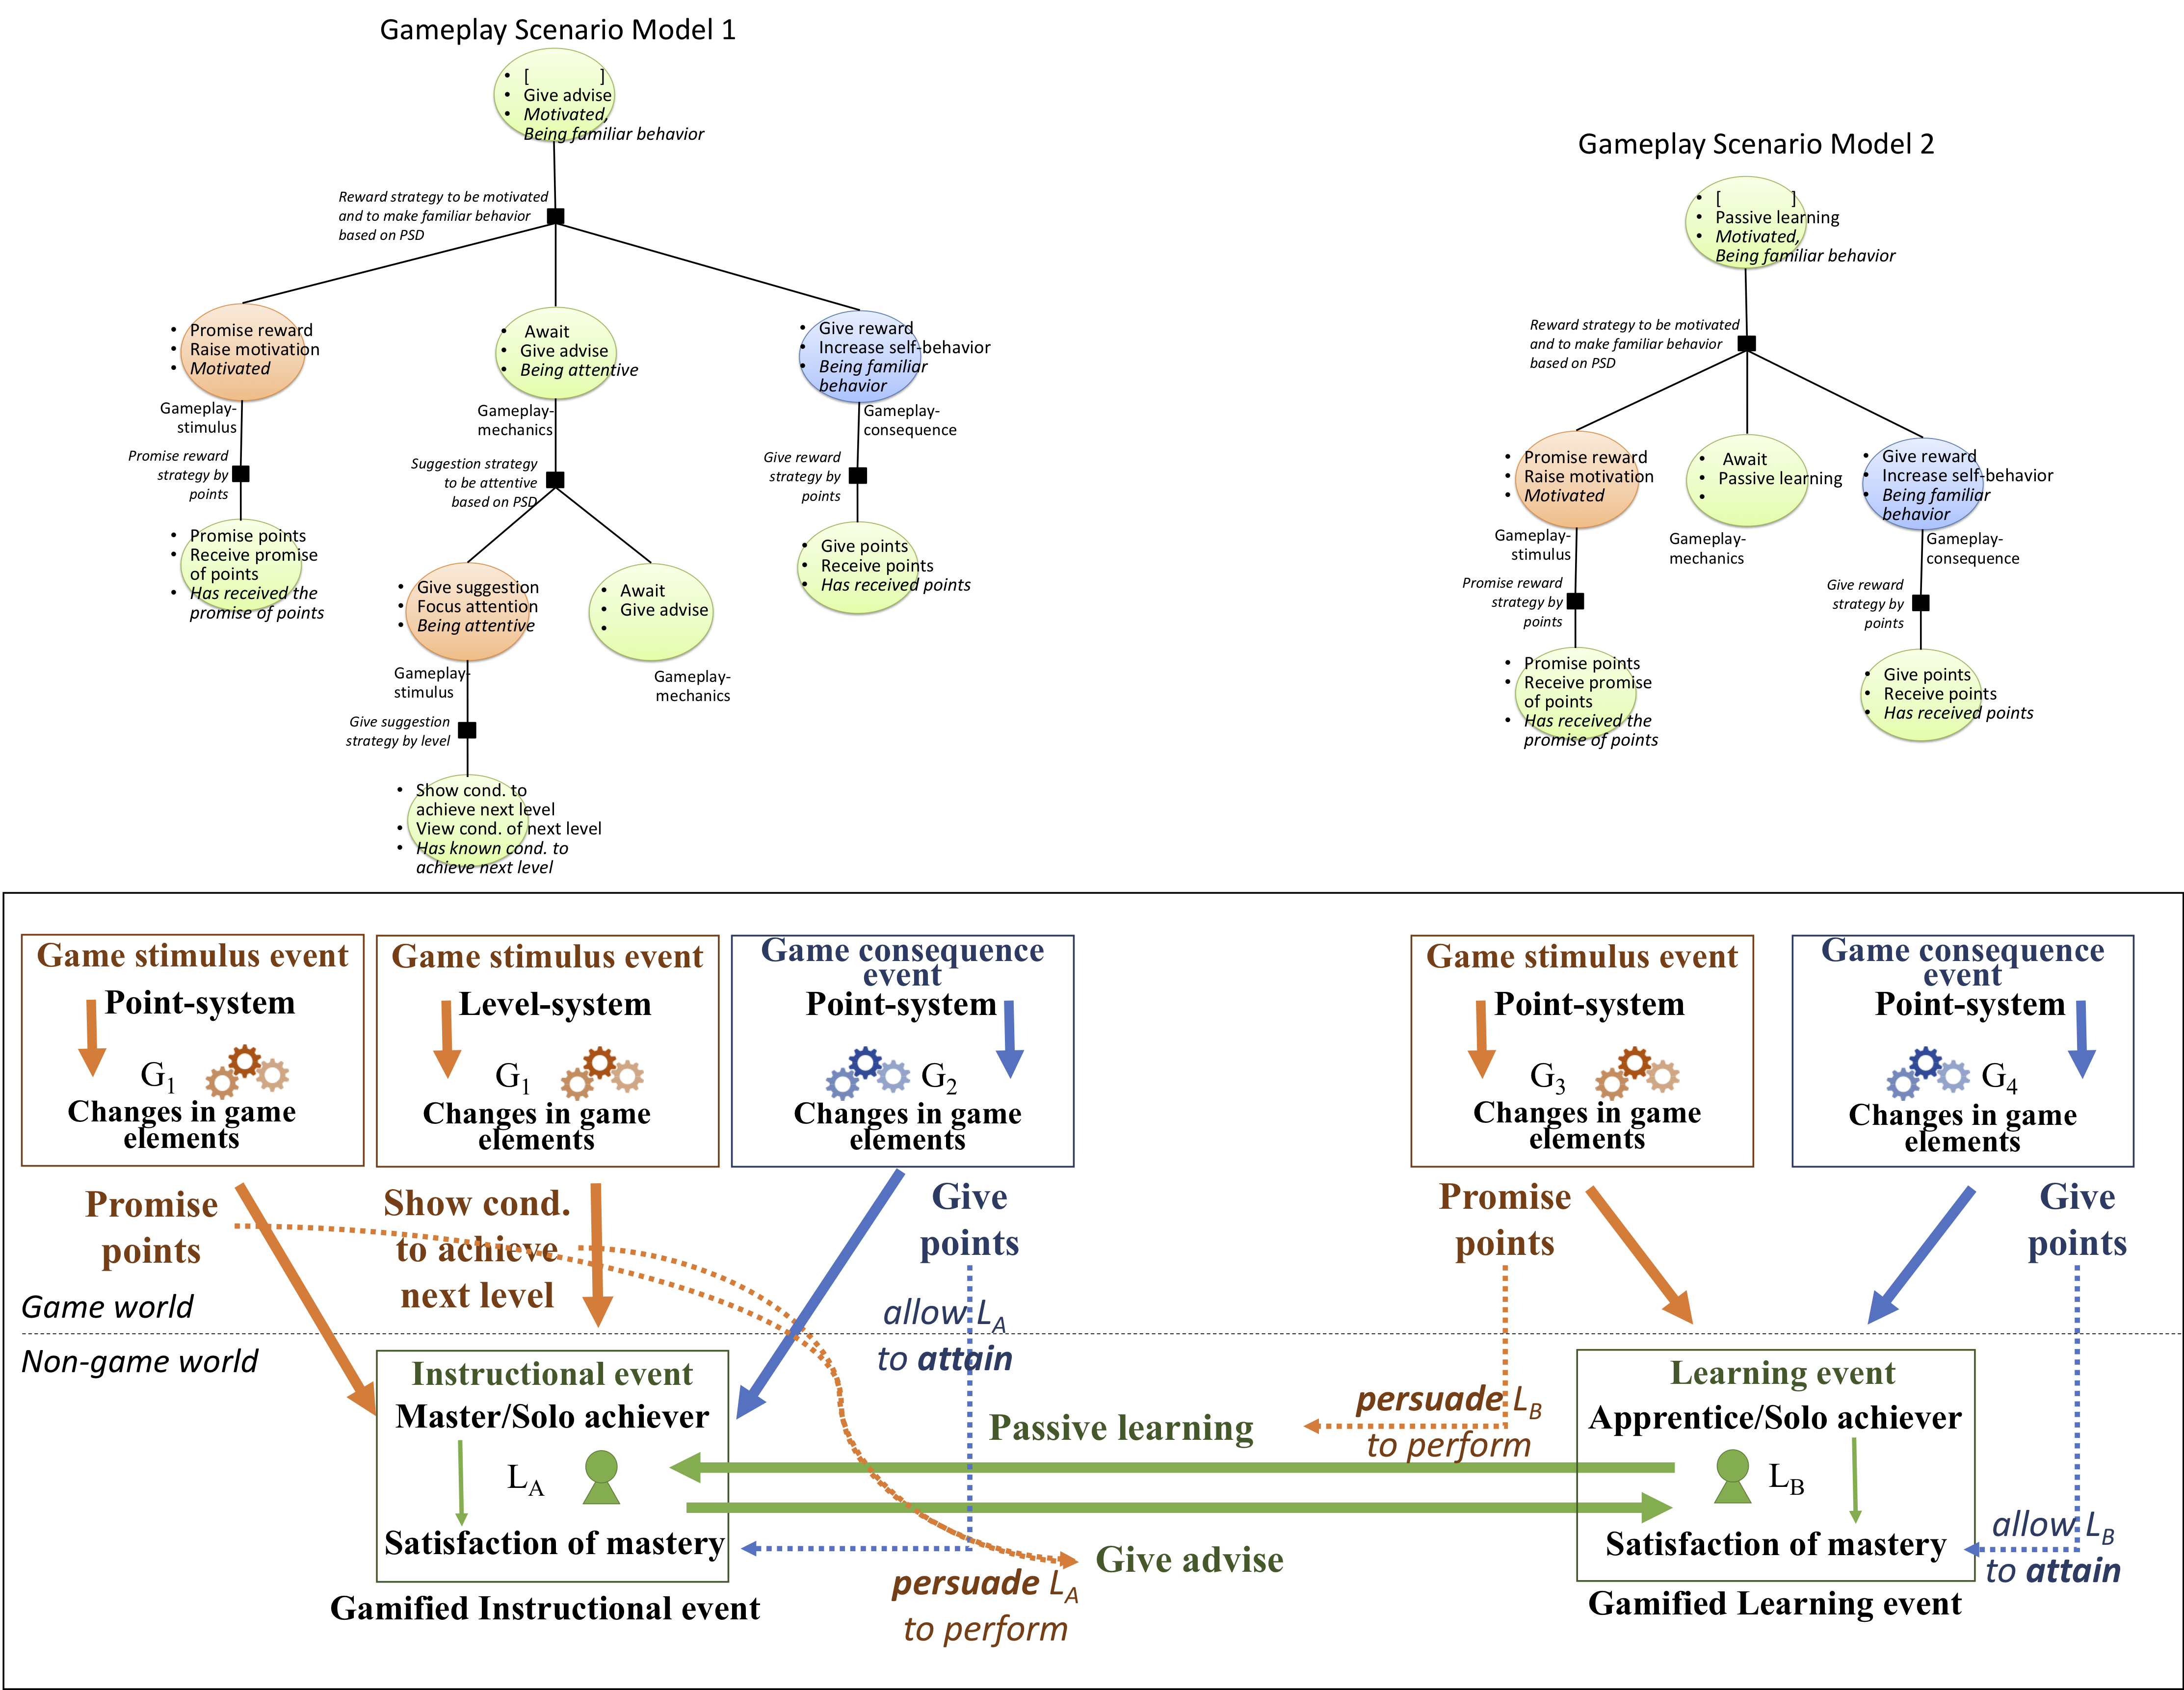
\includegraphics[width=1\textwidth]{images/chap-ontogacles2/elements-gamified-notify-how-learner-is.png}
 \fautor
\end{figure}

Having the representation of gamified I\_L events using ontological structures, there is the possibility to use the information contained in these structures to setting up the game elements introduced in the CL scenario being gamified.
Because the information is explicitly and formally represented in the ontological structures, the designer can use this information to establish the interactions between the game elements and participants in a CL scenario.
Thus, for the gamified I\_L event \aspas{\emph{Gamfied Notify how the learner is}} shown as an ontological structure at the bottom of \autoref{fig:ontological-structure-gamified-il-event} and with the elements illustrated in \autoref{fig:elements-gamified-notify-how-learner-is}, the interactions between participants and game elements can be established in the CL scenario according to the storyboard shown in \autoref{fig:storyboard-gamified-notify-how-learner-is}.
In this sense, the game actions \aspas{\emph{Promise points}} and \aspas{\emph{Show cond. to achieve next level}} indicated in the ontological structure as game stimuli are defined as the messages \aspas{\emph{Give advice, and gain +200 points}} and \aspas{\emph{400 points to achieve 2nd level}} to be given by a point-system and a level-system as shown in the screens (1A) and (1B).
These both messages must be displayed in the system before the instructional action \aspas{\emph{Give advice}} defined in the ontological structure as a game mechanism. Such instructional action is defined in the system as a message \aspas{\emph{Give advice indicating the learner's problem}} and an interactive form to be filled by the \emph{Master/Solo achiever role holders}.
The game action \aspas{\emph{Give points}} formalized as a game consequence in the ontological structure is setting up as the assignment of points and the message to be given to the \emph{Master/Solo achiever role holders} by the point-system as shown in the screen (3).

\begin{figure}[!htbp]
 \caption{Storyboard for the interactions between game elements and participants defined according to the example of gamified I\_L event \aspas{\emph{Gamified Notify how the learner is}.}}
 \label{fig:storyboard-gamified-notify-how-learner-is}
 \centering
 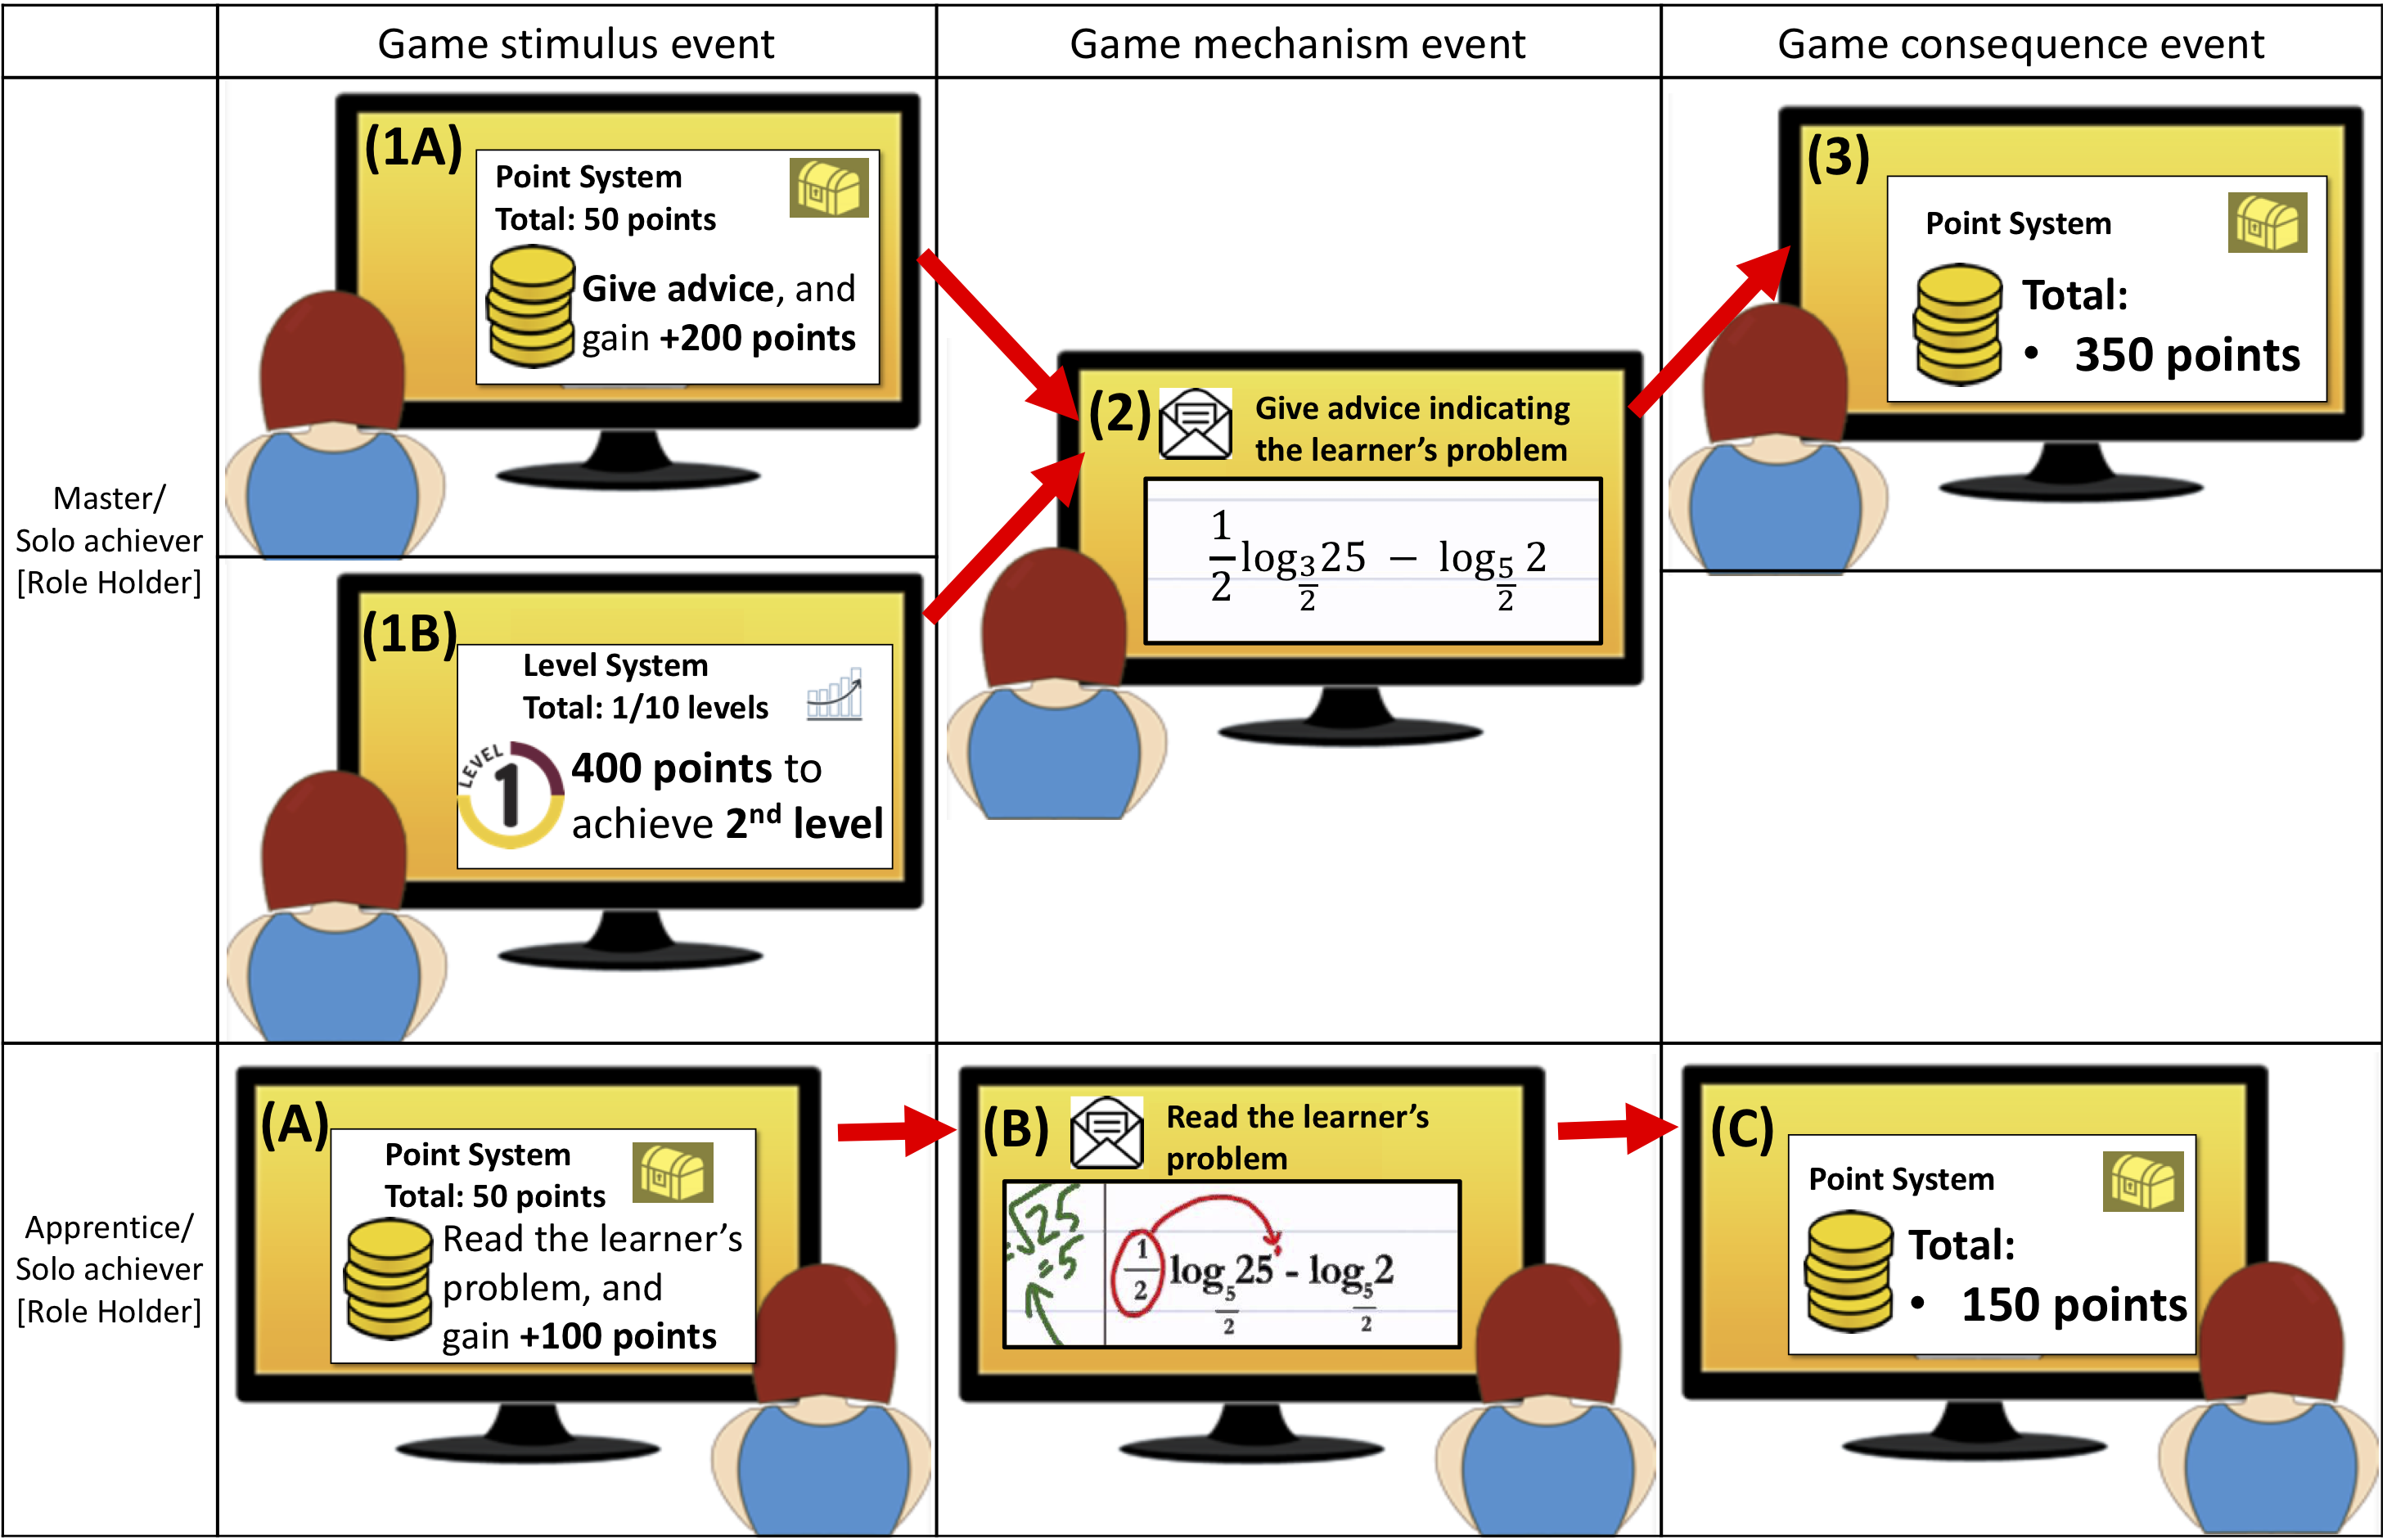
\includegraphics[width=0.85\textwidth]{images/chap-ontogacles2/storyboard-gamified-notify-how-learner-is.png}
 \fautor
\end{figure}

The configuration of game elements in the system for the \emph{Apprentice/Solo achiever role holder }is established as shown in the screens (A), (B) and (C) of \autoref{fig:storyboard-gamified-notify-how-learner-is}.
This configuration is established according to the information provided by the ontological structure shown at the bottom of \autoref{fig:ontological-structure-gamified-il-event}.
In this sense, the game action \aspas{\emph{Promise points}} as game stimulus is setting up as the message \aspas{\emph{Read the learner's problem and gain +100 points}} to be given by the point-system (Screen (A)), and the game action \aspas{\emph{Give points}} as game consequence is defined as the assignment of points and the message to be given by the point-system (Screen (C)).

The task of setting up the game actions to be performed by the game agents can be supported by an intelligent system that is able to reason on ontologies.
Thus, the designer just needs to have an elucidate idea of individual motivational goals (\emph{I-mot goal}) to be achieved by the instructor and learner in the gamified I\_L event.
These individual motivational goals represented as the contemplated \emph{Benefits for the players} in the ontological structures provide information to the intelligent system to find the game action that support the achievement of these benefits.
These game actions are actions indicated as game stimulus and game consequences in the gamified I\_L event, and they can be found by the intelligent system when it has the information of player roles and individual motivational goals assigned for the instructor and learner in a gamified CL scenario.
This process of extracting this information and how this information is used to setting up the game elements will be detailed in the \autoref{chapter:computer-based-mechanisms-procedures}.

\subsection{CL Game Dynamic}
\label{subsec:cl-game-dynamic}

According to the MDA framework proposed by \citeonline{HunickeLeBlancZubek2004}, the \aspas{\emph{Game dynamic describes the run-time behavior of the mechanics acting on player inputs and each others' outputs over time}} in which the mechanics describe the particular components of the game, at the level of data representation and algorithms. 
These mechanics have been represented as game agents in the ontological structures to represent game events as game stimulus and game consequence events in the gamified I\_L event.
Thus, to delineate the run-time behavior of these agents in a chunk of the CL process, in the ontological structure to represent a \emph{Gamified I\_L event}, the game events as \emph{game stimulus event} and \emph{game consequence event} include the description of these changes as object produced by the game actions and as states to be achieved by the game actions.
The green frame of \autoref{fig:ontological-structure-cl-game-dynamic} shows part of the formalization of the run-time behavior of the game agents in the game consequence events of a gamified instructional event.
As can be appreciated in the ontological structure to represent the CL Game dynamic, in the game stimulus event, the \emph{object} produced by the game action becomes \emph{Game component}, and the \emph{state} achieved by the game action becomes \emph{Game state}.

The piece of the whole CL process delimited by a gamified I\_L event is an interaction defined by the sequencing mechanism of a CSCL script.
Thus, to represent the game dynamic in the whole CL process, the concept of \aspas{\emph{CL Game dynamic}} has been formalized in the ontology OntoGaCLeS as \aspas{\emph{the run-time behavior of the game agents acting to persuade the participants to follow the interactions defined by the sequencing mechanism of a CSCL script}.}
At the top of \autoref{fig:ontological-structure-cl-game-dynamic} is shown the ontological structure to represent the CL Game dynamic in which the necessary and desired interactions are defined as roles that can be played by \emph{Gamified I\_L event}.
These interactions are defined from interaction patterns formalized in the CL ontology in which the interaction patterns are specialization of CSCL scripts inspired by instructional/learning theories.
An example of CL Game dynamic defined for the interaction pattern based on Cognitive Apprenticeship theory is shown at the bottom of \autoref{fig:ontological-structure-cl-game-dynamic}.
In this ontological structure named as \aspas{\emph{Gamified Cognitive Apprenticeship type IP},} the necessary interactions are: \emph{Gamified setting up learning context type CA}, \emph{Gamified demonstrating how to solve a problem}, \emph{Gamified monitoring}, and \emph{Gamified affirmative reaction}.
The desired interactions are: \emph{Gamified clarifying the problem}, \emph{Gamified notifying how the learner is}, \emph{Gamified instigating thinking}, \emph{Gamified requesting problem's details}, and \emph{Gamified showing a solution type CA}.

\begin{figure}[!htbp]
 \caption[Ontological structure to represent a \emph{CL Game dynamic}]{Ontological structure to represent the \aspas{\emph{CL Game dynamic}} (at the top). At the bottom, the ontological structure to represent a CL Game dynamic defined for the gamification of Cognitive Apprenticeship interaction pattern.}
 \label{fig:ontological-structure-cl-game-dynamic}
 \centering
 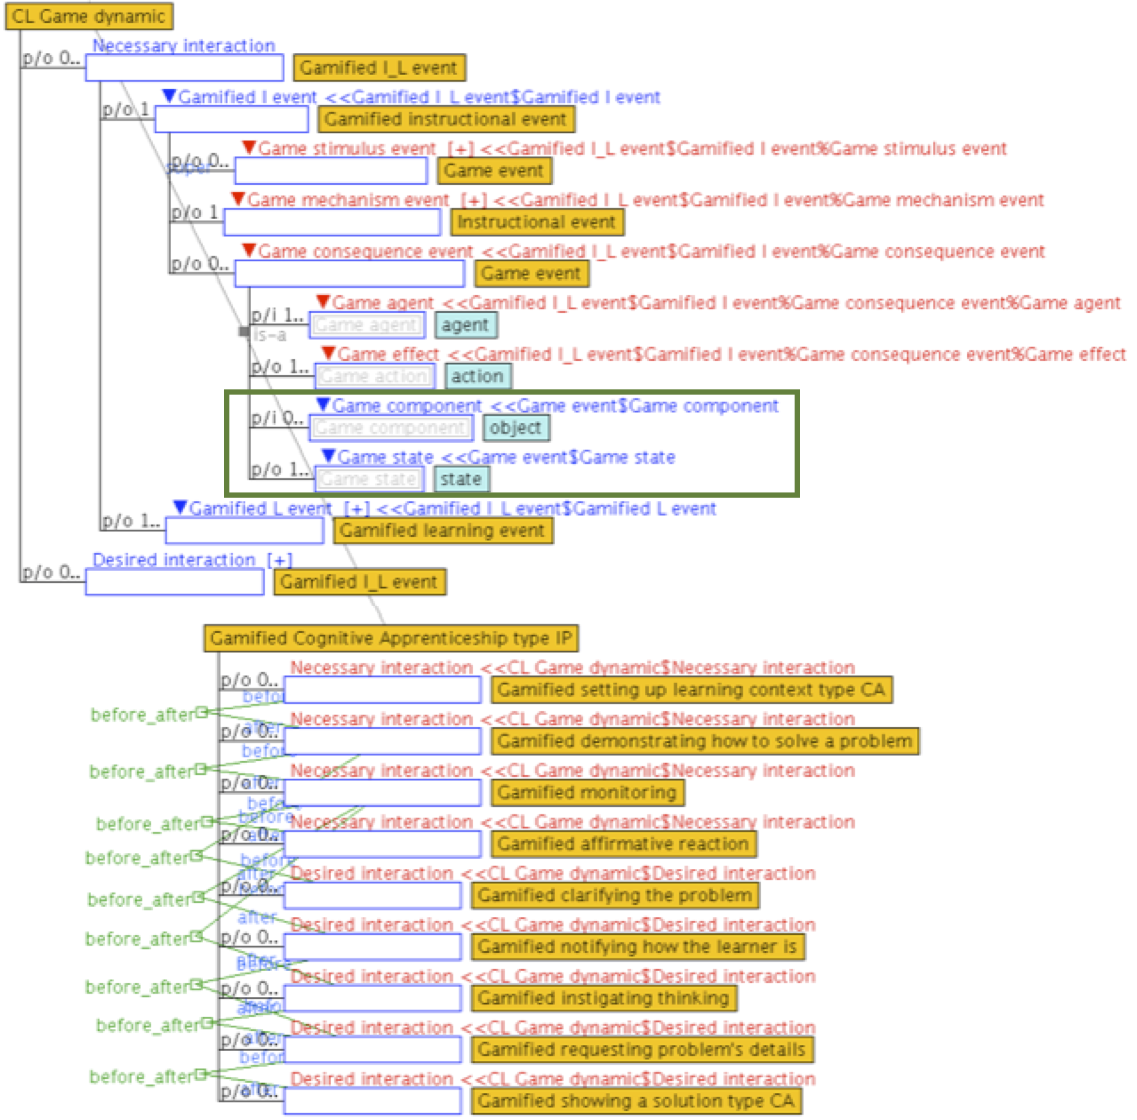
\includegraphics[width=1\textwidth]{images/chap-ontogacles2/ontological-structure-cl-game-dynamic.png}
 \fautor
\end{figure}

\subsection{CL Gameplay}
\label{subsec:cl-gameplay}

Beside the concept of gameplay is extensively talked in the literature related to game design and gamification, there is no one universally accepted definition of gameplay.
According to \citeonline{FabricatoreNussbaumRosas2002}, gamers talk about gameplay when they refer to their experiences in the game focusing on what the player can do, what the game elements can do in response to the player's actions.
Gameplay is the result of many contributing elements \cite{RollingsAdams2003}, thereby \citeonline{DjaoutiAlvarezJesselMethelMolinier2008} defines gameplay as the way in which the players interact with a game elements through rules listening input and acting on game elements.
These rules through the output system return to the player an evaluation of his performance observing the states of game elements. 

As the \emph{CL Game dynamic} delineates the run-time behavior of game elements to persuade the participants to follow the sequencing mechanism of a CSCL script, the gameplay of a gamified CL scenario, is the concept of \aspas{\emph{CL Gameplay},} consists in the set of CL game dynamics defined in this scenario to cause changes in the participants' attitudes, intentions, motivation and/or behaviors.
These changes are caused by the gameplay experience of participants interacting with the game elements through the CL Game dynamics.
Thus, in the ontological structure to represent a \emph{Gamified CL Scenarios} as shown in \autoref{fig:ontological-structure-cl-gameplay}, the \emph{CL process} is replaced by the \emph{CL Gameplay}, where the information about \aspas{\emph{How to interact}} in the CL process delineated by an \emph{Interaction pattern} is replaced by the \emph{CL Game dynamic} playing the role \aspas{\emph{How to play}.} 

\begin{figure}[!htbp]
 \caption[Ontological structure to represent a \emph{Gamified CL Scenario}]{Ontological structure to represent a \aspas{\emph{Gamified CL Scenario}.}}
 \label{fig:ontological-structure-cl-gameplay}
 \centering
 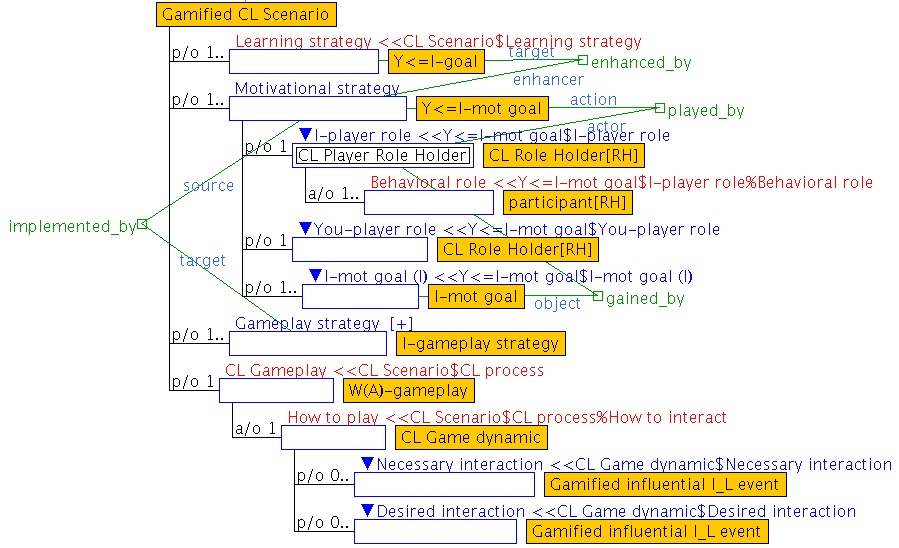
\includegraphics[width=0.95\textwidth]{images/chap-ontogacles2/ontological-structure-gamified-cl-scenario.png}
 \fautor
\end{figure}

%%%%%%%%%%%%%%%%%%%%%%%%%%%%%%%%%%%%%%%%%%%%%%%%%%
\section[Formalizing an Ontological Model to Apply Gamification as Persuasive Technology]{Formalizing an Ontological Model to Apply Gamification as Persuasive Technology in CL Scenarios}
\label{sec:formalizing-ontological-model-apply-gamification-persuasive-technology}

To demonstrate the applicability of the ontological structures presented in the previous sections, the building of an ontological model to apply gamification as persuasive technology in CL scenarios is detailed in this section.
By gamification as persuasive technology, the author of this thesis refers to the use of game design elements to persuade and social influence the participants to change their attitudes, intentions, motivation and/or behaviors.
Thus, an ontological model to apply gamification as persuasive technology in CL scenarios has the purpose to provide enough information for setting up the game elements to persuade the participants to follow the interactions defined by a CSCL script.
The ontological model detailed here has been proposed to apply gamification as persuasive technology in CL scenarios based on the Cognitive Apprenticeship theory, and the information used to build this model comes from the Yee's model \cite{Yee2006} and Model-driven persuasive game proposed by \citeonline{Orji2014}.

The steps for building an ontological model to apply gamification as persuasive in CL scenarios are:
(1) to identify the Persuasive Game Design Strategies (PGDSs) for player role holders who are in the \emph{primary focus} (P) and \emph{secondary focus} (S) of individual gameplay strategies (\emph{I-gameplay strategy});
(2) to apply the identified PGDSs in the interaction pattern; and
(3) to define the game states and game components in the CL Game Dynamics to provide a gameplay experience according to the individual gameplay strategies.

\subsubsection*{Step (1): Identifying persuasive game design strategies for player role holders who are in the primary focus and secondary focus of individual gameplay strategies}

Several researchers have pointed the necessity to personalize the application of persuasive strategies because of the adverse reactions that can be caused in a person when inappropriate strategies are applied.
For instance, a study of \citeonline{KapteinLacroixSaini2010} demonstrates that the use of non-tailored persuasive strategies produces negative reactions increasing the adoption of unhealthy behavior.
Another example is the study carried out by \citeonline{OrjiVassilevaMandryk2014} in which the effectiveness of PGDSs for player types of BrainHex model was evaluated to identify the best and worst strategies to motivate health behavior change.
Thus, to identifying the PGDSs for player role holders who are in the primary focus and secondary focus of individual gameplay strategies, it is necessary to have the list of PGDSs that cause positive and negative changes in the player roles of ontological model being built.
 
\autoref{tab:persuasive-strategies-model-driven-persuasive-game} shows the (P)ositive and (N)egative (counterproductive) effects for the player types of BrainHex model identified in the Model-driven persuasive game proposed by \citeonline{Orji2014}.
The PGDSs that cause the most (P)ositive and (N)egative effects for are indicated with bold texts.
The relation of BrainHex player types with the component motivations identified in the Yee's model is indicated in the column \aspas{\emph{Yee's Model},} and it has been extracted from the study of \citeonline{NackeBatemanMandryk2014} in which, for instance, the BrainHex's Mastermind player type is related to the Yee's \emph{Mechanics} component motivation because people who are classified in these both player types enjoys to devise strategies for solving puzzles and problem, because they obtain pleasure when they make good decisions.
The column \aspas{\emph{Player role}} indicates the relation between the PGDSs and the player roles based on the Yee's model.


\begin{quadro}[htb]
\caption{Persuasive game design strategies for player types of BrainHex and Yee's model}
\label{tab:persuasive-strategies-model-driven-persuasive-game}
\centering
\tiny
\begin{tabular}{|l|cccccccc|c|c|}
\hline

\multirow{2}{*}{\textbf{BrainHex}}&
\multirow{1}{*}{\textbf{CMPT/}}&
\multirow{2}{*}{\textbf{COOP}}&
\multirow{2}{*}{\textbf{CUST}}&
\multirow{2}{*}{\textbf{PERS}}&
\multirow{2}{*}{\textbf{PRAS}}&
\multirow{1}{*}{\textbf{SEMT/}}&
\multirow{2}{*}{\textbf{SIML}}&
\multirow{2}{*}{\textbf{REWD}}&
\multirow{2}{*}{\textbf{Yee's Model}}&
\multirow{2}{*}{\textbf{Player Role}}\tabularnewline
&
\multirow{1}{*}{\textbf{CMPR}}&
&
&
&
&
\multirow{1}{*}{\textbf{SUGG}}&
&
&
&
\tabularnewline
\hline

Achiever& &\textbf{(P)}& & & &(P)& &(P)&\emph{Advancement}&\multirow{3}{*}{Yee Achiever}\tabularnewline
Mastermind&(P)& &(P)&(P)& &\textbf{(P)}&(P)& &\emph{Mechanics}& \tabularnewline
Conqueror&\textbf{(P)}& & &(P)& &(P)&(P)& &\emph{Competition}& \tabularnewline
\hline

Socializer&(P)&\textbf{(P)}&(N)& &(N)&\textbf{(N)}& & &\emph{Social}&Yee Socializer\tabularnewline
\hline

Seeker&(P)& &\textbf{(P)}&(P)&(P)& & & &\emph{Immersion}&\multirow{3}{*}{Dreamer}\tabularnewline
Survivor&(P)&\textbf{(N)}&(N)& & &\textbf{(P)}& &(N)&\emph{Escapism}& \tabularnewline
Daredevil&(N)& & & & &\textbf{(N)}&\textbf{(P)}& &\emph{Escapism}& \tabularnewline
\hline

Achiever& &\textbf{(P)}& & & &(P)& &(P)&\emph{Advancement}&\multirow{4}{*}{Social Achiever}\tabularnewline
Mastermind&(P)& &(P)&(P)& &\textbf{(P)}&(P)& &\emph{Mechanics}& \tabularnewline
Conqueror&\textbf{(P)}& & &(P)& &(P)&(P)& &\emph{Competition}& \tabularnewline
Socializer&(P)&\textbf{(P)}&(N)& &(N)&\textbf{(N)}& & &\emph{Social}&\tabularnewline
\hline

Achiever& &\textbf{(P)}& & & &(P)& &(P)&\emph{Advancement}&\multirow{6}{*}{Achiever Dreamer}\tabularnewline
Mastermind&(P)& &(P)&(P)& &\textbf{(P)}&(P)& &\emph{Mechanics}& \tabularnewline
Conqueror&\textbf{(P)}& & &(P)& &(P)&(P)& &\emph{Competition}& \tabularnewline
Seeker&(P)& &\textbf{(P)}&(P)&(P)& & & &\emph{Immersion}&\tabularnewline
Survivor&(P)&\textbf{(N)}&(N)& & &\textbf{(P)}& &(N)&\emph{Escapism}& \tabularnewline
Daredevil&(N)& & & & &\textbf{(N)}&\textbf{(P)}& &\emph{Escapism}& \tabularnewline
\hline

Socializer&(P)&\textbf{(P)}&(N)& &(N)&\textbf{(N)}& & &\emph{Social}&\multirow{4}{*}{Social Dreamer}\tabularnewline
Seeker&(P)& &\textbf{(P)}&(P)&(P)& & & &\emph{Immersion}&\tabularnewline
Survivor&(P)&\textbf{(N)}&(N)& & &\textbf{(P)}& &(N)&\emph{Escapism}&\tabularnewline
Daredevil&(N)& & & & &\textbf{(N)}&\textbf{(P)}& &\emph{Escapism}&\tabularnewline
\hline

Achiever& &\textbf{(P)}& & & &(P)& &(P)&\emph{Advancement}&\multirow{7}{*}{Full Gamer}\tabularnewline
Mastermind&(P)& &(P)&(P)& &\textbf{(P)}&(P)& &\emph{Mechanics}& \tabularnewline
Conqueror&\textbf{(P)}& & &(P)& &(P)&(P)& &\emph{Competition}& \tabularnewline
Socializer&(P)&\textbf{(P)}&(N)& &(N)&\textbf{(N)}& & &\emph{Social}&\tabularnewline
Seeker&(P)& &\textbf{(P)}&(P)&(P)& & & &\emph{Immersion}&\tabularnewline
Survivor&(P)&\textbf{(N)}&(N)& & &\textbf{(P)}& &(N)&\emph{Escapism}& \tabularnewline
Daredevil&(N)& & & & &\textbf{(N)}&\textbf{(P)}& &\emph{Escapism}& \tabularnewline
\hline

\multicolumn{11}{r}{CMPT/CMPR: competition \& comparison, COOP: cooperation, CUST: customization, PERS: personalization, PRAS: praise,}\tabularnewline
\multicolumn{11}{r}{SEMT/SUGG: self-monitoring \& suggestion, SIML: simulation, REWD: reward}

\end{tabular}
\fautor
\end{quadro}


%\setlongtables{\tiny
%\begin{longtable}{|l|cccccccc|c|c|}
%\caption{Persuasive game design strategies for player types of BrainHex and Yee's model}
%\tabularnewline
%\hline\hline

%\endfirsthead\caption[]{\em (continued)} \tabularnewline
%\hline\hline
%\multirow{2}{*}{\textbf{BrainHex}}&
%\multirow{1}{*}{\textbf{CMPT/}}&
%\multirow{2}{*}{\textbf{COOP}}&
%\multirow{2}{*}{\textbf{CUST}}&
%\multirow{2}{*}{\textbf{PERS}}&
%\multirow{2}{*}{\textbf{PRAS}}&
%\multirow{1}{*}{\textbf{SEMT/}}&
%\multirow{2}{*}{\textbf{SIML}}&
%\multirow{2}{*}{\textbf{REWD}}&
%\multirow{2}{*}{\textbf{Yee's Model}}&
%\multirow{2}{*}{\textbf{Player Role}}\tabularnewline
%&
%\multirow{1}{*}{\textbf{CMPR}}&
%&
%&
%&
%&
%\multirow{1}{*}{\textbf{SUGG}}&
%&
%&
%&
%\tabularnewline
%\hline
%\endhead
%\hline

%\endfoot
%\label{tab:persuasive-strategies-model-driven-persuasive-game}


%\end{longtable}
%}

With the list of PGDSs that can be applied in the player roles, a combination of PGDSs is carried out for the player role holders who are in the primary focus and secondary focus of the individual gameplay strategies.
During this combination, the PGDSs that cause negative effects are avoided.
Thus, for example, for the player role holders: \aspas{\emph{Yee Achiever}} as primary focus (P), and \aspas{\emph{Socializer}} as secondary focus (S); the combination of PGDSs consists in the strategies of \emph{CMPT/CMPR}, \emph{COOP}, \emph{PERS}, \emph{SIML}, and \emph{REWD} in which the counterproductive PGDSs avoided for this combination were \emph{CUST}, and \emph{SEMT/SUGG} because these PGDSs have negative influence for the Yee Socializer player role.
\autoref{tab:pgds-cognitive-apprenticeship-yee-model} shows the combination of PGDSs for the player role holders based on the Yee's model.
Strike-through text in this table indicates a counterproductive PGDS. 


\newpage
\begin{landscape}

\begin{quadro}[htb]
\caption{Persuasive game design strategies for player role holders who are in the primary focus and secondary focus of individual gameplay strategies based on Yee's model}
\label{tab:pgds-cognitive-apprenticeship-yee-model}
\centering
\tiny
\begin{tabular}{|l|c|c|c|c|c|c|c|}
\hline
\multirow{1}{*}{\textbf{Primary focus (P)} x}&
\multirow{2}{*}{\textbf{Yee Socializer}}&
\multirow{2}{*}{\textbf{Yee Achiever}}&
\multirow{2}{*}{\textbf{Dreamer}}&
\multirow{2}{*}{\textbf{Social Achiever}}&
\multirow{2}{*}{\textbf{Achiever Dreamer}}&
\multirow{2}{*}{\textbf{Social Dreamer}}&
\multirow{2}{*}{\textbf{Full Gamer}}\tabularnewline
\multirow{1}{*}{\textbf{S-Player}}&
&
&
&
&
&
&
\tabularnewline
\hline\hline
%
\multirow{3}{*}{\textbf{Yee Socializer}}& 
\multicolumn{1}{|p{2.5cm}|}{\centering COOP, CMPT/CMPR}&%Yee Socializer
\multicolumn{1}{|p{2.5cm}|}{\centering COOP, CMPT/CMPR}&%Yee Achiever
\multicolumn{1}{|p{2.5cm}|}{\centering \st{COOP}, \st{CMPT/CMPR}}&%Dreamer
\multicolumn{1}{|p{2.5cm}|}{\centering COOP, CMPT/CMPR}&%Social Achiever
\multicolumn{1}{|p{2.5cm}|}{\centering \st{COOP}, \st{CMPT/CMPR}}&%Achiever Dreamer
\multicolumn{1}{|p{2.5cm}|}{\centering \st{COOP}, \st{CMPT/CMPR}}&%Social Dreamer
\multicolumn{1}{|p{2.5cm}|}{\centering \st{COOP}, \st{CMPT/CMPR}}\tabularnewline
& 
&
\multicolumn{1}{|p{2.5cm}|}{\centering x}&
\multicolumn{1}{|p{2.5cm}|}{\centering x}&
\multicolumn{1}{|p{2.5cm}|}{\centering x}&
\multicolumn{1}{|p{2.5cm}|}{\centering x}&
\multicolumn{1}{|p{2.5cm}|}{\centering x}&
\multicolumn{1}{|p{2.5cm}|}{\centering x}\tabularnewline
& 
&%Yee Socializer
\multicolumn{1}{|p{2.5cm}|}{\centering \mbox{\st{SEMT/SUGG}}, \mbox{CMPT/CMPR}, COOP, PERS, SIML, REWD, \st{CUST}}&%Yee Achiever
\multicolumn{1}{|p{2.5cm}|}{\centering SIML, PRAS, PERS}&%Dreamer
\multicolumn{1}{|p{2.5cm}|}{\centering CMPT/CMPR, COOP, PERS, SIML, REWD}&%Social Achiever
\multicolumn{1}{|p{2.5cm}|}{\centering SIML, PERS, \st{PRAS}}&%Achiever Dreamer
\multicolumn{1}{|p{2.5cm}|}{\centering SIML, PERS}&%Social Dreamer
\multicolumn{1}{|p{2.5cm}|}{\centering SIML, PERS}\tabularnewline
\hline

\multirow{3}{*}{\textbf{Yee Achiever}}& 
\multicolumn{1}{|p{2.5cm}|}{\centering \mbox{\st{SEMT/SUGG}}, \mbox{CMPT/CMPR}, COOP, PERS, SIML, REWD, \st{CUST}}&%Yee Socializer
\multicolumn{1}{|p{2.5cm}|}{\centering \mbox{SEMT/SUGG}, \mbox{CMPT/CMPR}, COOP, PERS, SIML, REWD, CUST} &%Yee Achiever
\multicolumn{1}{|p{2.5cm}|}{\centering \mbox{\st{SEMT/SUGG}}, \mbox{\st{CMPT/CMPR}}, \st{COOP}, PERS, SIML, \st{REWD}, \st{CUST}}&%Dreamer
\multicolumn{1}{|p{2.5cm}|}{\centering \mbox{\st{SEMT/SUGG}}, \mbox{CMPT/CMPR}, COOP, PERS, SIML, REWD, \st{CUST}}&%Social Achiever
\multicolumn{1}{|p{2.5cm}|}{\centering \mbox{\st{SEMT/SUGG}}, \mbox{\st{CMPT/CMPR}}, \st{COOP}, PERS, SIML, \st{REWD}, \st{CUST}}&%Achiever Dreamer
\multicolumn{1}{|p{2.5cm}|}{\centering \mbox{SEMT/SUGG}, \mbox{CMPT/CMPR}, COOP, PERS, SIML, REWD, CUST}&%Social Dreamer %%%%continue from here
\multicolumn{1}{|p{2.5cm}|}{\centering \mbox{SEMT/SUGG}, \mbox{CMPT/CMPR}, COOP, PERS, SIML, REWD, CUST}\tabularnewline
& 
\multicolumn{1}{|p{2.5cm}|}{\centering x}&
&
\multicolumn{1}{|p{2.5cm}|}{\centering x}&
\multicolumn{1}{|p{2.5cm}|}{\centering x}&
\multicolumn{1}{|p{2.5cm}|}{\centering x}&
\multicolumn{1}{|p{2.5cm}|}{\centering x}&
\multicolumn{1}{|p{2.5cm}|}{\centering x}\tabularnewline
& 
\multicolumn{1}{|p{2.5cm}|}{\centering COOP, CMPT/CMPR}&%Yee Socializer
&%Yee Achiever
\multicolumn{1}{|p{2.5cm}|}{\centering SIML, PRAS, PERS}&%Dreamer
\multicolumn{1}{|p{2.5cm}|}{\centering CMPT/CMPR, COOP, PERS, SIML, REWD}&%Social Achiever
\multicolumn{1}{|p{2.5cm}|}{\centering SIML, PERS, PRAS}&%Achiever Dreamer
\multicolumn{1}{|p{2.5cm}|}{\centering SIML, PERS}&%Social Dreamer
\multicolumn{1}{|p{2.5cm}|}{\centering SIML, PERS}\tabularnewline
\hline


\multirow{3}{*}{\textbf{Dreamer}}& 
\multicolumn{1}{|p{2.5cm}|}{\centering SIML, PRAS, PERS}&
\multicolumn{1}{|p{2.5cm}|}{\centering SIML, PRAS, PERS} &
\multicolumn{1}{|p{2.5cm}|}{\centering SIML, PRAS, PERS}&
\multicolumn{1}{|p{2.5cm}|}{\centering SIML, PRAS, PERS}&
\multicolumn{1}{|p{2.5cm}|}{\centering SIML, PRAS, PERS}&
\multicolumn{1}{|p{2.5cm}|}{\centering SIML, PRAS, PERS}&
\multicolumn{1}{|p{2.5cm}|}{\centering SIML, PRAS, PERS}\tabularnewline
& 
\multicolumn{1}{|p{2.5cm}|}{\centering x}&
\multicolumn{1}{|p{2.5cm}|}{\centering x}&
&
\multicolumn{1}{|p{2.5cm}|}{\centering x}&
\multicolumn{1}{|p{2.5cm}|}{\centering x}&
\multicolumn{1}{|p{2.5cm}|}{\centering x}&
\multicolumn{1}{|p{2.5cm}|}{\centering x}\tabularnewline
& 
\multicolumn{1}{|p{2.5cm}|}{\centering \st{COOP}, \st{CMPT/CMPR}}&%Yee Socializer
\multicolumn{1}{|p{2.5cm}|}{\centering \mbox{\st{SEMT/SUGG}}, \mbox{\st{CMPT/CMPR}}, \st{COOP}, PERS, SIML, \st{REWD}, \st{CUST}}&%Yee Achiever
&%Dreamer
\multicolumn{1}{|p{2.5cm}|}{\centering CMPT/CMPR, COOP, PERS, SIML, REWD}&%Social Achiever
\multicolumn{1}{|p{2.5cm}|}{\centering SIML, PERS, PRAS}&%Achiever Dreamer
\multicolumn{1}{|p{2.5cm}|}{\centering SIML, PERS}&%Social Dreamer
\multicolumn{1}{|p{2.5cm}|}{\centering SIML, PERS}\tabularnewline
\hline


\multirow{3}{*}{\textbf{Social Achiever}}& 
\multicolumn{1}{|p{2.5cm}|}{\centering CMPT/CMPR, COOP, PERS, SIML, REWD}&%Yee Socializer
\multicolumn{1}{|p{2.5cm}|}{\centering CMPT/CMPR, COOP, PERS, SIML, REWD}&%Yee Achiever
\multicolumn{1}{|p{2.5cm}|}{\centering CMPT/CMPR, COOP, PERS, SIML, REWD}&%Dreamer
\multicolumn{1}{|p{2.5cm}|}{\centering CMPT/CMPR, COOP, PERS, SIML, REWD}&%Social Achiever
\multicolumn{1}{|p{2.5cm}|}{\centering CMPT/CMPR, COOP, PERS, SIML, REWD}&%Achiever Dreamer
\multicolumn{1}{|p{2.5cm}|}{\centering CMPT/CMPR, COOP, PERS, SIML, REWD}&%Social Dreamer
\multicolumn{1}{|p{2.5cm}|}{\centering CMPT/CMPR, COOP, PERS, SIML, REWD}\tabularnewline
& 
\multicolumn{1}{|p{2.5cm}|}{\centering x}&
\multicolumn{1}{|p{2.5cm}|}{\centering x}&
\multicolumn{1}{|p{2.5cm}|}{\centering x}&
&
\multicolumn{1}{|p{2.5cm}|}{\centering x}&
\multicolumn{1}{|p{2.5cm}|}{\centering x}&
\multicolumn{1}{|p{2.5cm}|}{\centering x}\tabularnewline
& 
\multicolumn{1}{|p{2.5cm}|}{\centering COOP, CMPT/CMPR}&%Yee Socializer
\multicolumn{1}{|p{2.5cm}|}{\centering \mbox{\st{SEMT/SUGG}}, \mbox{CMPT/CMPR}, COOP, PERS, SIML, REWD, \st{CUST}}&%Yee Achiever
\multicolumn{1}{|p{2.5cm}|}{\centering SIML, PRAS, PERS}&%Dreamer
&%Social Achiever
\multicolumn{1}{|p{2.5cm}|}{\centering SIML, PERS, PRAS}&%Achiever Dreamer
\multicolumn{1}{|p{2.5cm}|}{\centering SIML, PERS}&%Social Dreamer
\multicolumn{1}{|p{2.5cm}|}{\centering SIML, PERS}\tabularnewline
\hline
%\newpage
\multicolumn{8}{r}{CMPT/CMPR: competition \& comparison, COOP: cooperation, CUST: customization, PERS: personalization, PRAS: praise,}\tabularnewline
\multicolumn{8}{r}{SEMT/SUGG: self-monitoring \& suggestion, SIML: simulation, REWD: reward}
\end{tabular}
\fautor
\end{quadro}

\newpage

%\begin{quadro}[htb]
%\caption{Persuasive game design}
\centering
\tiny
\begin{tabular}{|l|c|c|c|c|c|c|c|}
\hline
\multirow{1}{*}{\textbf{Primary focus (P)} x}&
\multirow{2}{*}{\textbf{Yee Socializer}}&
\multirow{2}{*}{\textbf{Yee Achiever}}&
\multirow{2}{*}{\textbf{Dreamer}}&
\multirow{2}{*}{\textbf{Social Achiever}}&
\multirow{2}{*}{\textbf{Achiever Dreamer}}&
\multirow{2}{*}{\textbf{Social Dreamer}}&
\multirow{2}{*}{\textbf{Full Gamer}}\tabularnewline
\multirow{1}{*}{\textbf{S-Player}}&
&
&
&
&
&
&
\tabularnewline
\hline\hline
%

\multirow{3}{*}{\textbf{Achiever Dreamer}}& 
\multicolumn{1}{|p{2.5cm}|}{\centering SIML, PRAS, \st{PERS}}&%Yee Socializer
\multicolumn{1}{|p{2.5cm}|}{\centering SIML, PRAS, PERS}&%Yee Achiever
\multicolumn{1}{|p{2.5cm}|}{\centering SIML, PRAS, PERS}&%Dreamer
\multicolumn{1}{|p{2.5cm}|}{\centering SIML, PRAS, PERS}&%Social Achiever
\multicolumn{1}{|p{2.5cm}|}{\centering SIML, PRAS, PERS}&%Achiever Dreamer
\multicolumn{1}{|p{2.5cm}|}{\centering SIML, PRAS, PERS}&%Social Dreamer
\multicolumn{1}{|p{2.5cm}|}{\centering SIML, PRAS, PERS}\tabularnewline
& 
\multicolumn{1}{|p{2.5cm}|}{\centering x}&
\multicolumn{1}{|p{2.5cm}|}{\centering x}&
\multicolumn{1}{|p{2.5cm}|}{\centering x}&
\multicolumn{1}{|p{2.5cm}|}{\centering x}&
&
\multicolumn{1}{|p{2.5cm}|}{\centering x}&
\multicolumn{1}{|p{2.5cm}|}{\centering x}\tabularnewline
& 
\multicolumn{1}{|p{2.5cm}|}{\centering \st{COOP}, \st{CMPT/CMPR}}&%Yee Socializer
\multicolumn{1}{|p{2.5cm}|}{\centering \mbox{\st{SEMT/SUGG}}, \mbox{\st{CMPT/CMPR}}, \st{COOP}, PERS, SIML, \st{REWD}, \st{CUST}}&%Yee Achiever
\multicolumn{1}{|p{2.5cm}|}{\centering SIML, PRAS, PERS}&%Dreamer
\multicolumn{1}{|p{2.5cm}|}{\centering CMPT/CMPR, COOP, PERS, SIML, REWD}&%Social Achiever
&%Achiever Dreamer
\multicolumn{1}{|p{2.5cm}|}{\centering SIML, PERS}&%Social Dreamer
\multicolumn{1}{|p{2.5cm}|}{\centering SIML, PERS}\tabularnewline
\hline

\multirow{3}{*}{\textbf{Social Dreamer}}& 
\multicolumn{1}{|p{2.5cm}|}{\centering SIML, PERS}&%Yee Socializer
\multicolumn{1}{|p{2.5cm}|}{\centering SIML, PERS}&%Yee Achiever
\multicolumn{1}{|p{2.5cm}|}{\centering SIML, PERS}&%Dreamer
\multicolumn{1}{|p{2.5cm}|}{\centering SIML, PERS}&%Social Achiever
\multicolumn{1}{|p{2.5cm}|}{\centering SIML, PERS}&%Achiever Dreamer
\multicolumn{1}{|p{2.5cm}|}{\centering SIML, PERS}&%Social Dreamer
\multicolumn{1}{|p{2.5cm}|}{\centering SIML, PERS}\tabularnewline
& 
\multicolumn{1}{|p{2.5cm}|}{\centering x}&
\multicolumn{1}{|p{2.5cm}|}{\centering x}&
\multicolumn{1}{|p{2.5cm}|}{\centering x}&
\multicolumn{1}{|p{2.5cm}|}{\centering x}&
\multicolumn{1}{|p{2.5cm}|}{\centering x}&
&
\multicolumn{1}{|p{2.5cm}|}{\centering x}\tabularnewline
& 
\multicolumn{1}{|p{2.5cm}|}{\centering \st{COOP}, \st{CMPT/CMPR}}&%Yee Socializer
\multicolumn{1}{|p{2.5cm}|}{\centering \mbox{SEMT/SUGG}, \mbox{CMPT/CMPR}, COOP, PERS, SIML, REWD, CUST}&%Yee Achiever
\multicolumn{1}{|p{2.5cm}|}{\centering SIML, PRAS, PERS}&%Dreamer
\multicolumn{1}{|p{2.5cm}|}{\centering CMPT/CMPR, COOP, PERS, SIML, REWD}&%Social Achiever
\multicolumn{1}{|p{2.5cm}|}{\centering SIML, PRAS, PERS}&%Achiever Dreamer
&%Social Dreamer
\multicolumn{1}{|p{2.5cm}|}{\centering SIML, PERS}\tabularnewline
\hline

\multirow{3}{*}{\textbf{Full Gamer}}& 
\multicolumn{1}{|p{2.5cm}|}{\centering SIML, PERS}&%Yee Socializer
\multicolumn{1}{|p{2.5cm}|}{\centering SIML, PERS}&%Yee Achiever
\multicolumn{1}{|p{2.5cm}|}{\centering SIML, PERS}&%Dreamer
\multicolumn{1}{|p{2.5cm}|}{\centering SIML, PERS}&%Social Achiever
\multicolumn{1}{|p{2.5cm}|}{\centering SIML, PERS}&%Achiever Dreamer
\multicolumn{1}{|p{2.5cm}|}{\centering SIML, PERS}&%Social Dreamer
\multicolumn{1}{|p{2.5cm}|}{\centering SIML, PERS}\tabularnewline
& 
\multicolumn{1}{|p{2.5cm}|}{\centering x}&
\multicolumn{1}{|p{2.5cm}|}{\centering x}&
\multicolumn{1}{|p{2.5cm}|}{\centering x}&
\multicolumn{1}{|p{2.5cm}|}{\centering x}&
\multicolumn{1}{|p{2.5cm}|}{\centering x}&
\multicolumn{1}{|p{2.5cm}|}{\centering x}&
\tabularnewline
& 
\multicolumn{1}{|p{2.5cm}|}{\centering \st{COOP}, \st{CMPT/CMPR}}&%Yee Socializer
\multicolumn{1}{|p{2.5cm}|}{\centering \mbox{SEMT/SUGG}, \mbox{CMPT/CMPR}, COOP, PERS, SIML, REWD, CUST}&%Yee Achiever
\multicolumn{1}{|p{2.5cm}|}{\centering SIML, PRAS, PERS}&%Dreamer
\multicolumn{1}{|p{2.5cm}|}{\centering CMPT/CMPR, COOP, PERS, SIML, REWD}&%Social Achiever
\multicolumn{1}{|p{2.5cm}|}{\centering SIML, PRAS, PERS}&%Achiever Dreamer
\multicolumn{1}{|p{2.5cm}|}{\centering SIML, PERS}&%Social Dreamer
\tabularnewline
\hline
\multicolumn{8}{r}{CMPT/CMPR: competition \& comparison, COOP: cooperation, CUST: customization, PERS: personalization, PRAS: praise,}\tabularnewline
\multicolumn{8}{r}{SEMT/SUGG: self-monitoring \& suggestion, SIML: simulation, REWD: reward}
\end{tabular}
%\fautor
%\end{quadro}


\end{landscape}

\subsubsection*{Step (2): Applying persuasive game design strategies in the interaction pattern}

The PGDSs identified in the step (1) can be applied in the instructional and learning events to gamify them by the definition of \emph{Persuasive Gameplay Scenario Models} as was detailed in \autoref{subsec:persuasive-gameplay-scenario-model}.
The PGDSs indicated in the primary focus (P) can be applied in the instructional events of the interaction pattern, and the PGDSs indicated in the secondary focus (S) can be applied in the learning events of the interaction pattern.
The application of PGDSs for the pairs of instructional and learner events in an interaction pattern is formalized as gamified I\_L events to define the CL Game dynamics of the ontological model being built.

With the information of PGDSs shown in \autoref{tab:pgds-cognitive-apprenticeship-yee-model}, an ontological model to apply gamification as persuasive technology in CL scenarios based on the Cognitive Apprenticeship theory and with the player roles based on the Yee's model has been formalized in the ontology OntoGaCLeS to engender gameplay experiences of individual and cooperative competition.
This model consists in the following ontological structures to represent gamified CL scenarios:
(1) an ontological structure \aspas{\emph{Gamified Cognitive Apprenticeship Scenario for Master/Yee Achiever and Apprentice/Yee Achiever}} to support a CL Gameplay experience of individual competition;
(2) an ontological structure {\emph{Gamified Cognitive Apprenticeship Scenario for Master/Yee Socializer and Apprentice/Yee Socializer}} to support a CL Gameplay experience of cooperative competition; and
(3) an ontological structure \aspas{\emph{Gamified Cognitive Apprenticeship Scenario for Master/Social Achiever and Apprentice/Social Achiever}} to support a CL gameplay experience of individual and cooperative competition. 

\autoref{fig:ontological-structure-cognitive-apprenticeship-master-achiever-apprentice-achiever} shows the ontological structure formalized to represent a \emph{Gamified Cognitive Apprenticeship Scenario for Master/Social Achiever and Apprentice/Social Achiever}.
In this structure, the motivational strategy \aspas{\emph{Gamify for Yee Achievers}} has been defined as the strategy to enhance the learning strategies \aspas{\emph{Learning by Guiding}} and \aspas{\emph{Learning by Apprenticeship}} assigned to the master and apprentices, respectively. The motivational strategy \aspas{\emph{Gamifying for Yee Achievers}} is implemented by the individual gameplay strategy \aspas{\emph{Ind CMPT gameplay strategy with REWD for CUST/EXPL}} to allow the apprentice role holders to attain the \emph{Satisfaction of competence} and \emph{Internalization of intrinsic motivation} as individual motivation goals (\emph{I-mot goal}).
According to this individual gameplay strategy, to provide an individual competition with rewards for customize avatars and explore new content, the game elements that should be introduced in the CL scenario for apprentices with the Yee achiever role holder are: a \emph{Game Point system (individual)} that is a game point system with individual points, a \emph{Game Level/Progression system (individual)} that is a game level system based on the individual progression of participant, a \emph{Game Leaderboard system (individual ranking)} that is a leaderboard with individual rankings, a \emph{Game Custom system} as a system to provide items for customizing elements of system, and a \emph{Game Discovery system} as a system to provide support for exploring new content in the system.

\begin{figure}[!htbp]
 \caption[Ontological structure to represent a \emph{Gamified Cognitive Apprenticeship Scenario for Master/Yee Achiever and Apprentice/Yee Achiever}]{Ontological structure to represent a \aspas{\emph{Gamified Cognitive Apprenticeship Scenario for Master/Yee Achiever and Apprentice/Yee Achiever}.}}
 \label{fig:ontological-structure-cognitive-apprenticeship-master-achiever-apprentice-achiever}
 \centering
 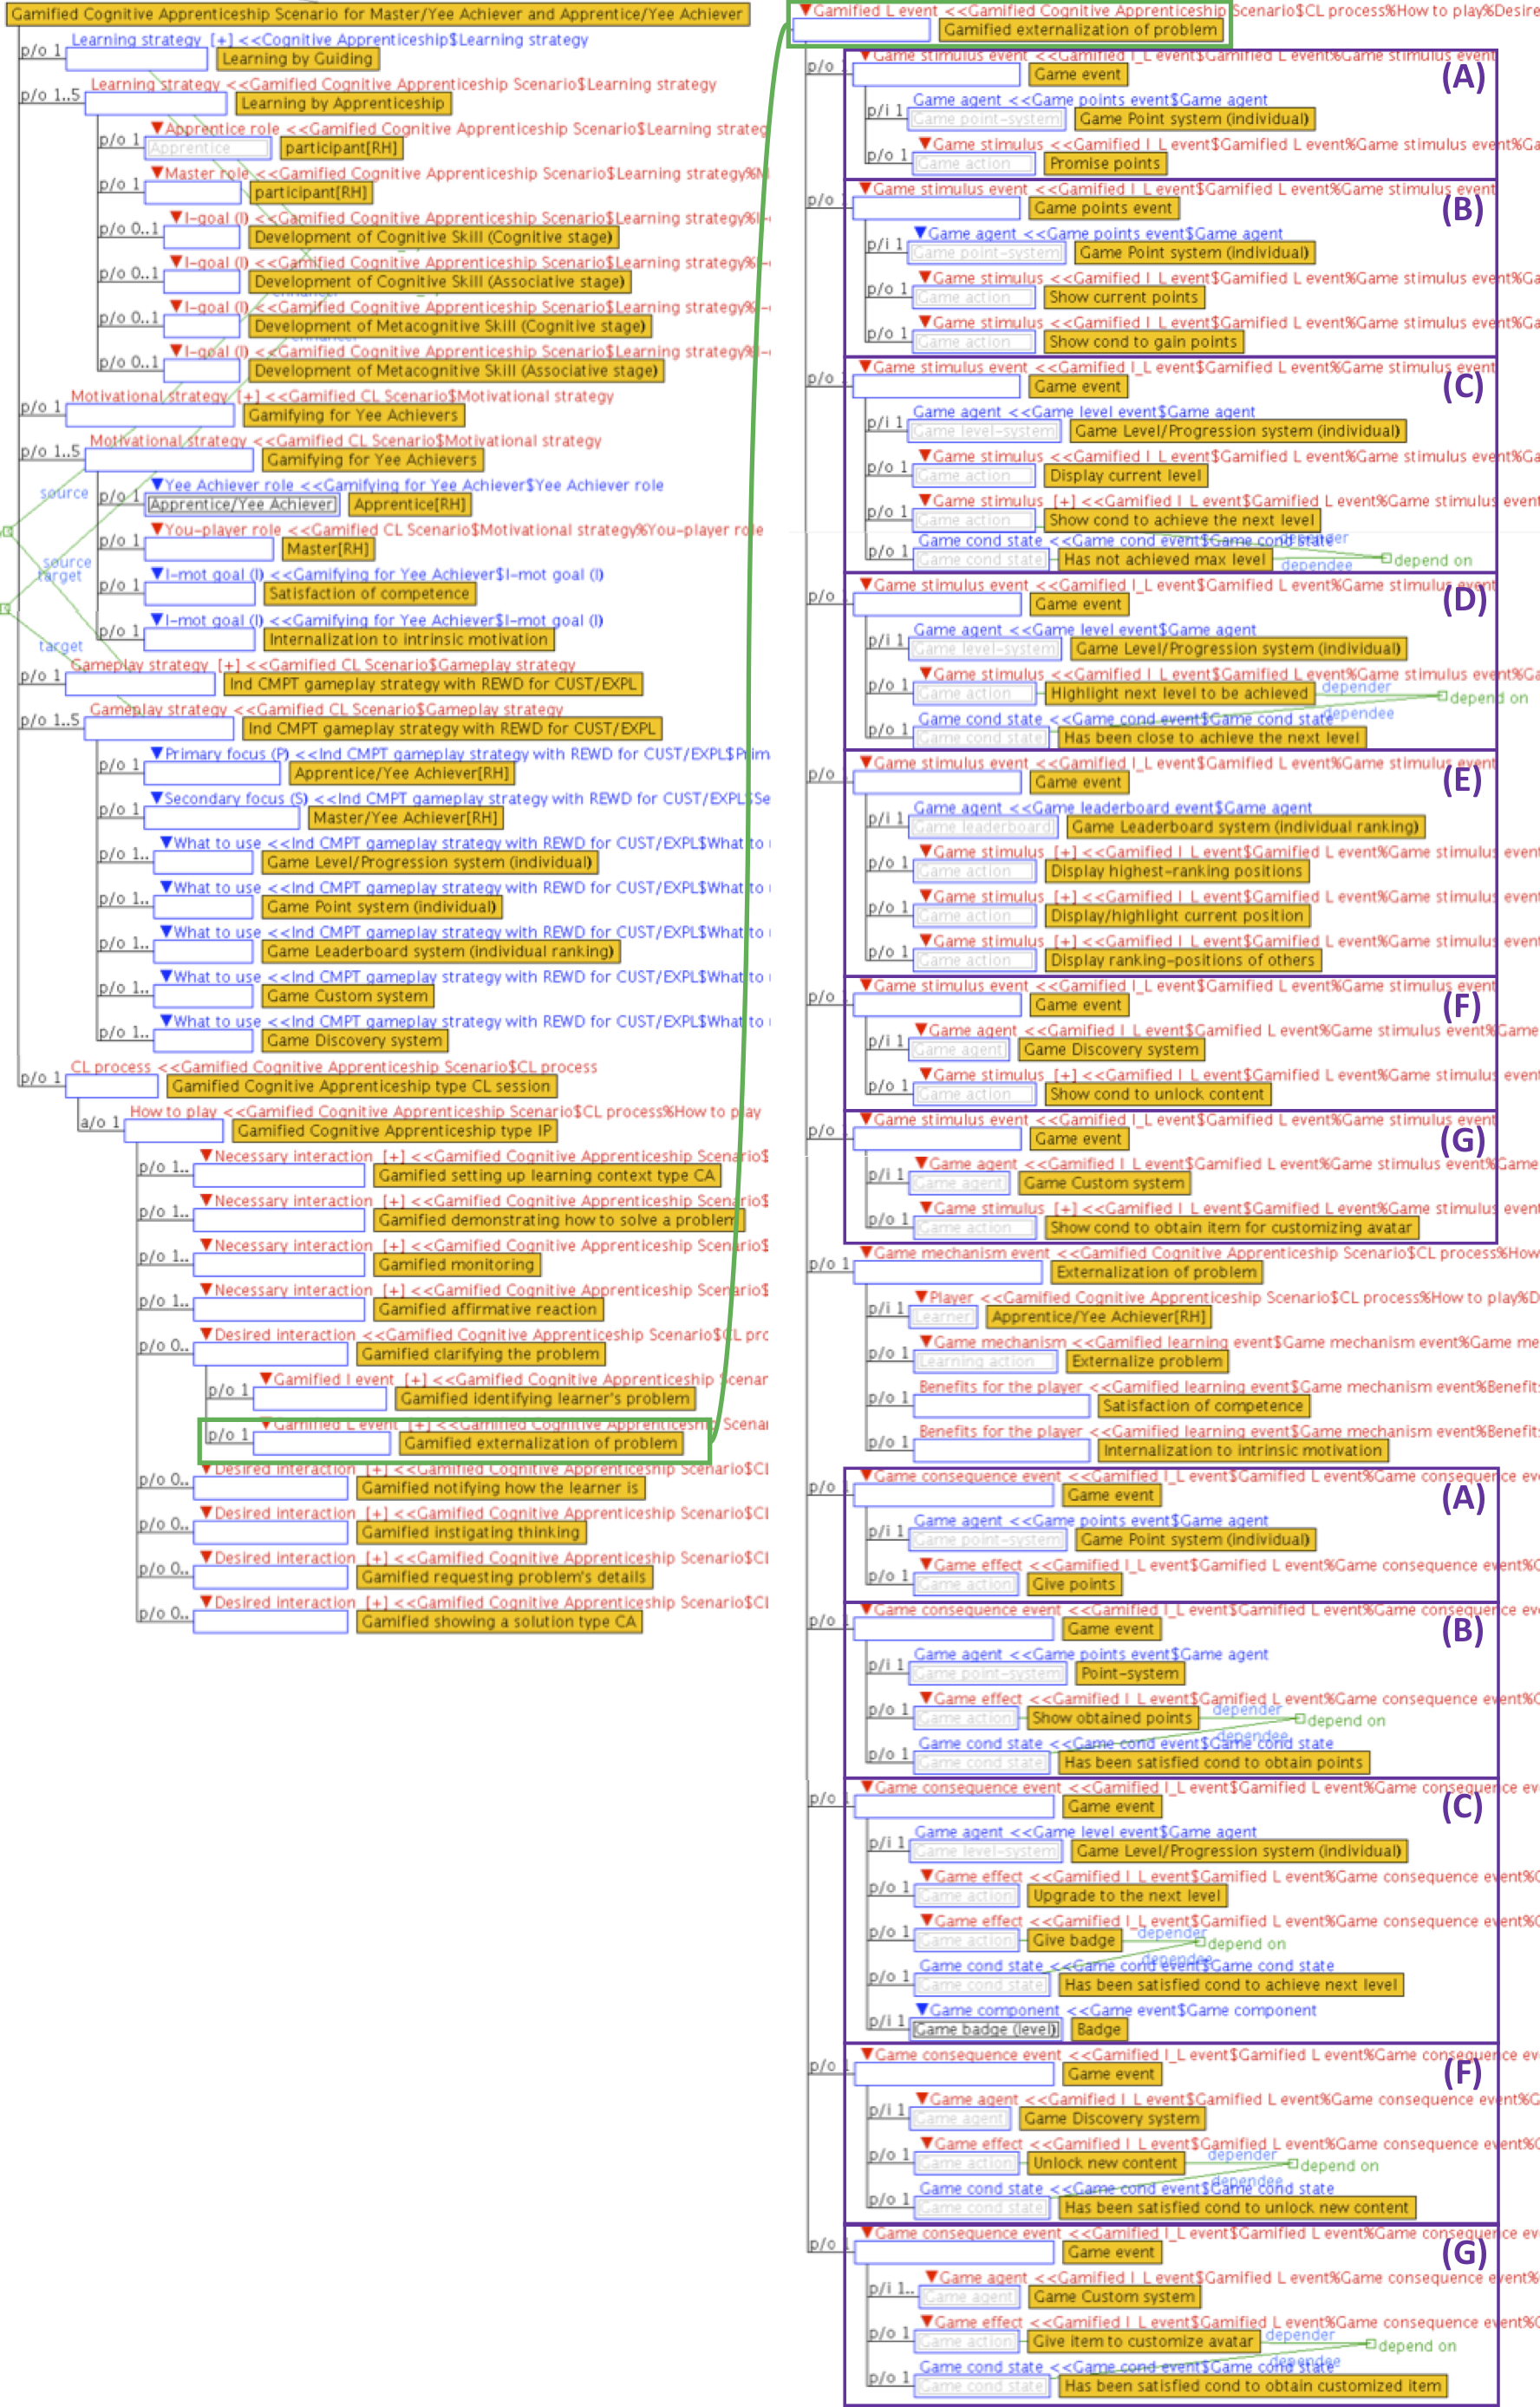
\includegraphics[width=0.95\textwidth]{images/chap-ontogacles2/ontological-structure-cognitive-apprenticeship-master-achiever-apprentice-achiever.png}
 \fautor
\end{figure}
\newpage

%%%%

On the right side of \autoref{fig:ontological-structure-cognitive-apprenticeship-master-achiever-apprentice-achiever} is detailed the gamified learning event \aspas{\emph{Gamified externalization of problem}} that is result of applying the combination of PGDSs \aspas{\emph{SEMT/SUGG, CMPT/CMPR, COOP, PERS, SIM, REWD, CUST}} to gamify the learning event \aspas{\emph{Externalization of problem}.}
The application of the PGDS \aspas{\emph{Reward strategy based on PDS}} in the game element \aspas{\emph{Game Point system (individual)}} defined the game stimulus and consequence events indicated by the frames (A). According to these events, the game action defined as game stimulus is \aspas{\emph{Promise points},} and the game action defined as game effect is: \aspas{\emph{Give points}.}
By applying the PGDSs \aspas{\emph{Self-monitoring strategy based on PDS}} and \aspas{\emph{Suggestion strategy based on the PDS}} in the game element \aspas{\emph{Game Point system (individual)},} the game stimulus and consequence events indicated in the frames (B) were obtained, where the game actions \aspas{\emph{Show current points}} and \aspas{\emph{Show cond to gain points}} are game stimulus, and the game action \aspas{\emph{Show obtained points}} is a game effect.
The game actions \aspas{\emph{Display current level}} and \aspas{\emph{Show cond to achieve the next level}} as game stimulus, and the game action \aspas{\emph{Upgrade to the next level}} as game effect were result of applying the PGDSs \aspas{\emph{Self-monitoring strategy based on PDS}} and \aspas{\emph{Suggestion strategy based on the PDS}} in the game element \aspas{\emph{Game Level/Progression system (individual)}}.
These game stimulus and game effects formalized as game events are shown in the frames (C).
By applying the PGDS \aspas{\emph{Simulation strategy based on the PDS}} in the game element \aspas{\emph{Game Level/Progression system (individual)},} the game stimulus event showed in the frame (D) has been formalized as the game action \aspas{\emph{Highlight next level to be achieved}} when a participant \emph{Has been close to achieve the next level}.
The game stimulus event showed in the frame (E) with the game actions \aspas{\emph{Display highest-ranking positions},} \aspas{\emph{Display/highlight current position}} and \aspas{\emph{Display ranking-positions of others}} has been obtained by the application of PGDSs \aspas{\emph{Competition strategy based on the PDS}} and \aspas{\emph{Comparison strategy based on the PDS}} in the game element \aspas{\emph{Game Leaderboard system (individual ranking)}.}
The application of the PGDS \aspas{\emph{Personalization strategy based on PDS}} in the game element \aspas{\emph{Game Custom system}} defined the game stimulus and consequence events shown in the frames (F), where the game action \aspas{\emph{Show cond to unlock content}} is defined as a game stimulus, and where the game action \aspas{\emph{Unlock new content}} is defined as game effect.
Finally, the game stimulus and consequence events showed in the frame (G) has been obtained by the application of the PGDS \aspas{\emph{Customization strategy based on PDS}} in the game element \aspas{\emph{Game Discovery system},} where the game action \aspas{\emph{Show cond to obtain item for customizing avatar}} is a game stimulus, and the game action \aspas{\emph{Give item to customize avatar}} is a game effect.

\subsubsection*{Step (3): Defining the game states and game components in the CL Game dynamic to provide a gameplay experience according to the individual gameplay strategies}
 
The last step in the formalization of ontological models to apply gamification as persuasive technology consists in the definition of game states and game components in the CL Game dynamic to connect the selected game elements. This connection is also established by setting of the game action in the game stimulus and consequence events.
To engender a gameplay experience of individual competition for the Master/Yee Achiever role holders in the \aspas{\emph{Gamified Cognitive Apprenticeship Scenario for Master/Yee Achiever and Apprentice/Yee Achiever},} \emph{Game Level/Progression system (individual)} is connected to the \emph{Game Point system (individual)} by setting of the condition to achieve the next level in the game action \aspas{\emph{Show cond to achieve the next level}} as shown in \autoref{fig:ontological-structures-connection-gameplay-experience} (A), where the condition \aspas{\emph{Has obtained [n] individual game points}} is defined as a state to be achieved by the \emph{Apprentice/Yee Achiever role holder} (\emph{owner}) \emph{from} a \emph{Game Point system (individual)}.
The game element \aspas{\emph{Game Leaderboard system (individual ranking)}} is connected to the \aspas{\emph{Game Point system (individual)}} to define individual rankings based on the individual points as shown in \autoref{fig:ontological-structures-connection-gameplay-experience} (B).

\begin{figure}[!htbp]
 \caption[Connection of game elements to establish a gameplay experience of individual competition in the \emph{Gamified Cognitive Apprenticeship Scenario for Master/Yee Achiever and Apprentice/Yee Achiever}]{Connection of game elements to establish a gameplay experience of individual competition in the \aspas{\emph{Gamified Cognitive Apprenticeship Scenario for Master/Yee Achiever and Apprentice/Yee Achiever}.}}
 \label{fig:ontological-structures-connection-gameplay-experience}
 \centering
 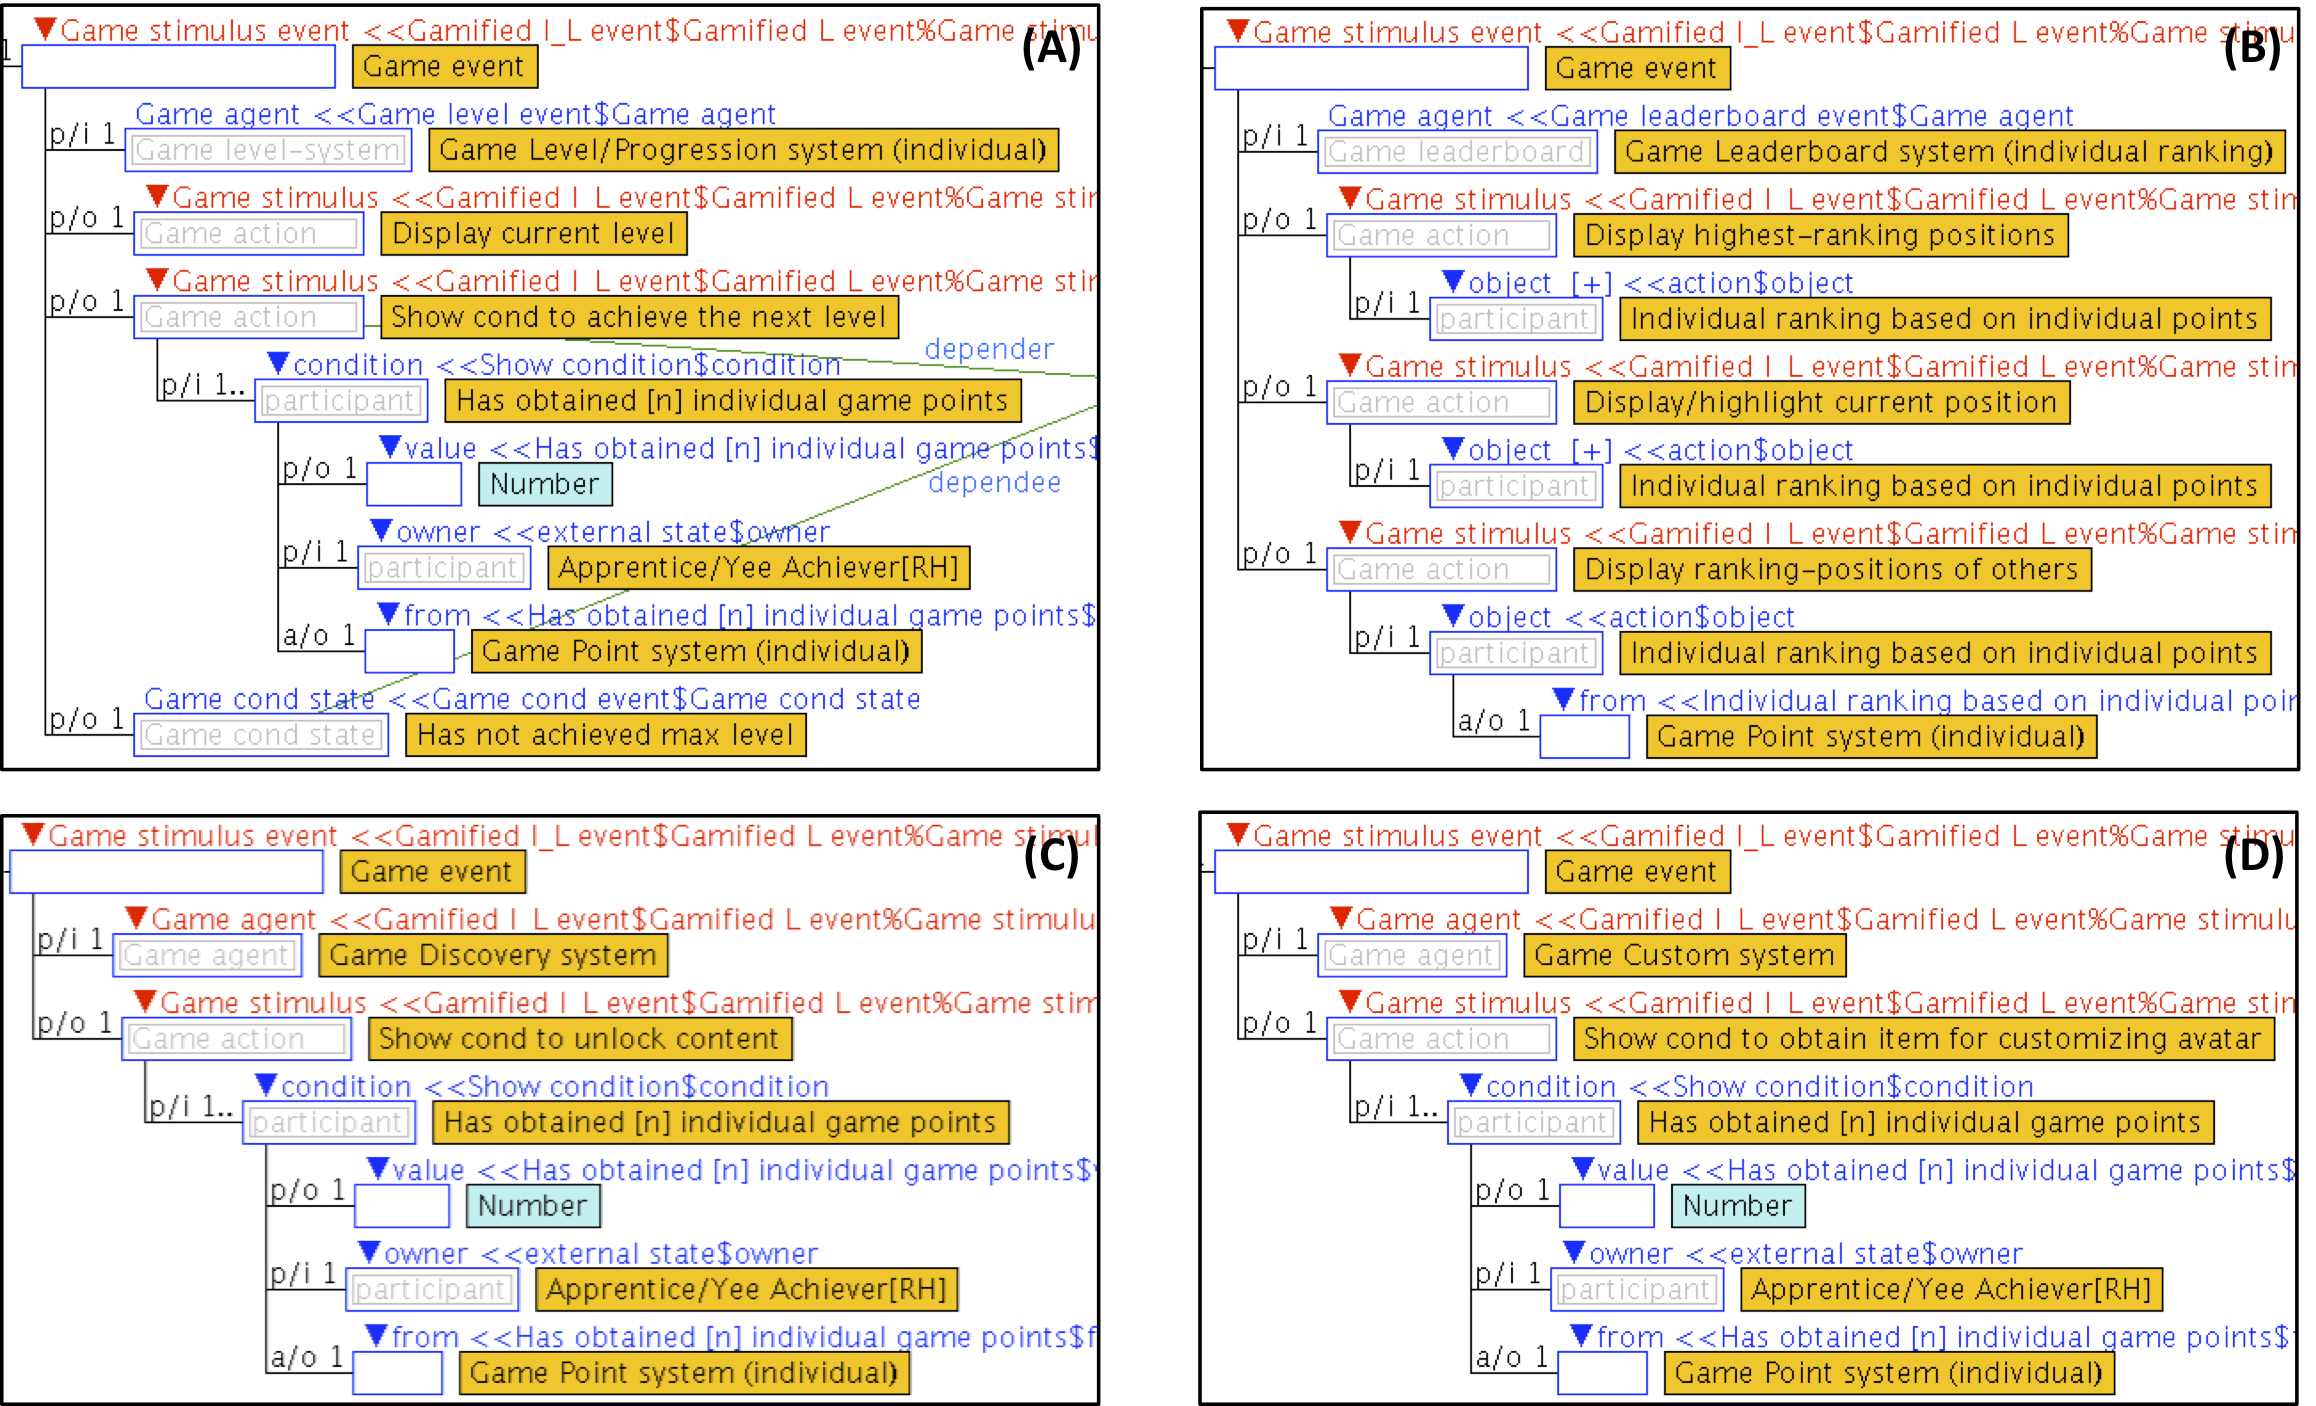
\includegraphics[width=0.95\textwidth]{images/chap-ontogacles2/ontological-structures-connection-gameplay-experience.png}
 \fautor
\end{figure}

\autoref{fig:ontological-structures-connection-gameplay-experience} (C) shows the setting for the connection between the game elements \aspas{\emph{Game Point system (individual)}} and \aspas{\emph{Game Discovery system}} in which the condition \aspas{\emph{Has obtained [n] individual game points}} for the game stimulus \aspas{\emph{Show cond to unlock content}} is established as the state owns by the \emph{Apprentice/Yee Achiever role holder} (\emph{owner}) given \emph{from} the \emph{Game Point system (individual)}.
This connection is defined to unlock new content in the system when the master achiever role holder gained [n] points.
The configuration to give items for customizing avatar is show in \autoref{fig:ontological-structures-connection-gameplay-experience} (D), where the condition to perform the game action \aspas{\emph{Show cond to obtain item for customizing avatar}} is that the apprentice achiever role holder \aspas{\emph{Has obtained [n] individual game points}.} Thus, the attribute-of (\emph{a/o}) \aspas{\emph{from}} has been defined as \emph{Game Point system (individual)}, and the owner role is played by the \aspas{\emph{Apprentice/Yee Achiever[RH]}.}

%%%%%%%%%%%%%%%%%%%%%%%%%%%%%%%%%%%%%%%%%%%%%%%%%%
\section{Concluding Remarks}
\label{sec:ontogacles2-concluding-remarks} 

Gamification as persuasive technology has been formalized in this chapter as the application of Persuasive Game Design Strategies (PGDSs) in non-game events to gamify them.
Thus, to represent the knowledge involved in this process as ontological structures, the author of this thesis has proposed a nested structure of non-game world, game world and gamification world to identify, classify and differentiate the elements related to non-game events and game events.
With this classification, the link between the Persuasive Game Design (PGD) and the design of CL process is represented in explicitly form by \emph{gameplay events}.
The prescriptive representation of the link between PGD and the design of CL process has been formalized through \emph{WAY-knowledge of PGDS}.
This formalization is accomplished through the representation of \aspas{\emph{What}} and \aspas{\emph{How}} to achieve expected changes in person's attitudes, intentions, motivations and/or behaviors to persuade him/her to perform the actions specified in the non-game events.
The design rationale in the application of PGDs to gamify a non-game event has been formalized as the concept of \aspas{\emph{Gameplay Scenario Model},} and it is used to gamify instructional and learning events defined in interactions patterns based on the sequencing mechanism of a CSCL script.
Thus, the pairs of gamified instructional and learning events have been formalized as ontological structures under the concept of \emph{Gamified I\_L event} to represent an interaction in the CL process.
As result of the application of PGDSs in the interaction pattern, a \emph{CL Game dynamic} is obtained to establish a \emph{CL Gameplay} in a gamified CL scenario. 

The usefulness of the ontological structures proposed here has been demonstrated by the formalization of an ontological model to apply gamification as persuasive technology in gamified CL scenarios based on the Cognitive Apprenticeship theory and with the player roles based on the Yee's model.
The application of PGDSs to apply gamification as persuasive technology has the purpose to engender gameplay experiences of individual and cooperative competition based on the information extracted from the Model-driven persuasive game proposed by \citeonline{Orji2014}. 

To solve the context-dependency of gamification in CL scenarios to persuade the participants to follow the interactions defined by the sequencing mechanism of a CSCL script, computer-based mechanisms can be built to help the design of CL gameplay in gamified CL scenarios.
This support is given by information extracted from ontological models to apply gamification as persuasive technology in which the ontological structures to represent gamified I\_L events are used to establish the interactions between participants and game elements in the environment to run the gamified CL scenarios.
Employing the formalization of WAY-knowledge of PGDS, computer-based mechanisms that support the building of a WAY-knowledge base of PGDSs can be built and computer-based mechanism that support the building of ontological models to apply gamification as persuasive technology in gamified CL scenarios.
These computer based mechanism will be presented in \autoref{chapter:computer-based-mechanisms-procedures}. 

\chapter[A Unify Modeling of Learner's Growth Process and Flow Theory]{A Unify Modeling of Learner's Growth Process and Flow Theory}
\label{chapter:unify-modeling-learner-growth-flow-theory}

In the learning process, the affective state of students plays an essential role that influences several mechanisms of rational thinking and learning \cite{DMello2012, Picard2000, ReisRodriguezLyraJaquesBittencourtIsotani2015}. Students with negative affective states (e.g. boredom) during the learning process are, in general, significantly more likely to obtain inadequate learning outcomes, because they often are not motivated and are not engaged in the learning process \cite{CraigGraesserSullinsGholson2004, ShernoffCsikszentmihalyiSchneiderShernoff2014}. In this sense, to motivate a student so that he/she participates in a learning scenario with complete immersion, it is necessary that his/her affective state provide an optimal experience. This affective state is denominated flow, and it is a mental state of operation characterized by a feeling of energized focus, full involvement, and success in the task being performed \cite{Csikszentmihalyi2008}. 

To define a gamified CL scenario with game elements that favor and maintain the participants in the flow state during the CL process, it is necessary to have understanding about the influence of these game elements in the affective state of participants. One condition for attaining and maintaining the flow state is the good balance between the perceived challenges of the tasks that will be carried out, and the participant’s own perceived abilities to accomplish these tasks. A task that is perceived too challenging or one that is not challenging enough may lead to anxiety or boredom, and when a person perceives that he/she does not have enough ability or he/she has too ability to carry out the task, he/she would be anxious or bored. Thus, a model known as GMIF model: \aspas{\emph{Learner’s \textbf{G}rowth \textbf{M}odel \textbf{I}mproved by \textbf{F}low Theory}} to integrate the learner's growth process and the third condition of good balance between the perceived challenges and ability is presented in this chapter. 

This chapter is organized as follows: The first section provides details about the Learner’s Growth Model (LGM model) and the three-channel flow model (\autoref{sec:lgm-model-three-channel-flow-model}). Then, the GMIF model is presented in \autoref{sec:integrating-learners-growth-model-flow-theory}. To demonstrate the usefulness of the GMIF model, \autoref{sec:application-giving-rewards-by-gimf-model} illustrates how this model can be used to establish the game rewards that will be given to the participants in a gamified CL scenario to maintain them in the flow state. Finally, \autoref{sec:model-gmif-concluding-remarks} presents the concluding remarks.

Part of the work described in this chapter was published by the author of this PhD thesis dissertation in the scientific article:

\begin{itemize}
\item
\aspas{\emph{Toward A Unified Modeling of Learner's Growth Process and Flow Theory}} published in the International Journal of Educational Technology \& Society, Vol. 19, No. 2, April 2016 \cite{ChallcoAndradeBorgesBittencourtIsotani2016}.
\end{itemize}

%%%%%%%%%%%%%%%%%%%%%%%%%%%%%%%%%%%%%%%%%%%%%%%%%%

\section{Learner’s Growth Model and Three-channel Flow Model}
\label{sec:lgm-model-three-channel-flow-model}

\subsection{Learner’s Growth Model}
\label{subsec:learners-growth-model}

Based on learning theories, the \aspas{\emph{\textbf{L}earners \textbf{G}rowth \textbf{M}odel}} (LGM model) is a graph that represents the learning process of a student as stages of skill development and knowledge acquisition as a directed graph \cite{InabaIkedaMizoguchi2003, IsotaniMizoguchi2006}. The learner’s growth process is represented as paths on the graph that allow for the representation of the relationships between learning strategies and their educational benefits.

As shown in \autoref{fig:lgm-model}, the LGM model has twenty states that are the result of the number of stages related to skill development multiplied by the number of stages related to knowledge acquisition. In the graph, the stages of skill development (nothing, rough cognitive, explanatory cognitive, associative, and autonomous) are represented in the lower-left triangle, while the stages of knowledge acquisition (nothing, accretion, tuning, and restructuring) are represented in the upper-right triangle. In skill development, the cognitive stage (rough, and explanatory) involves an initial encoding of a target skill that allows the learner to present the desired behavior or, at least, some rough approximation thereof; the associative stage is the improvement of the desired skill through practice; and the autonomous stage involves gradual continued improvement in the performance of the skill \cite{Anderson1982}. During knowledge acquisition, the accretion stage incorporates the addition and interpretation of new information in terms of pre-existent knowledge; the tuning stage involves coming to understand the knowledge through its application in a specific situation; and the restructuring stage comprises a process in which the relationship of the acquired knowledge is considered and the existent knowledge structure is rebuilt \cite{RumelhartNorman1976}.

The arrows in the LGM model shown in \autoref{fig:lgm-model} represent possible transitions between stages, and the form $s(x,y)$ on the top of each vertex is the simplified form of representing a stage, where the symbol \aspas{$x$} represents the current stage of skill development, and the symbol \aspas{$y$} represents the current stage of knowledge acquisition. For instance, the transition $s(0,0) \to s(2,0)$ means the possible transition from the stage $s(0,0)$ where a learner does not have any knowledge or skills to the associative stage $s(2,0)$ of skill development.

 \begin{figure}[htb]
 \caption{Learner’s Growth Model (LGM model)}
 \label{fig:lgm-model}
 \centering
 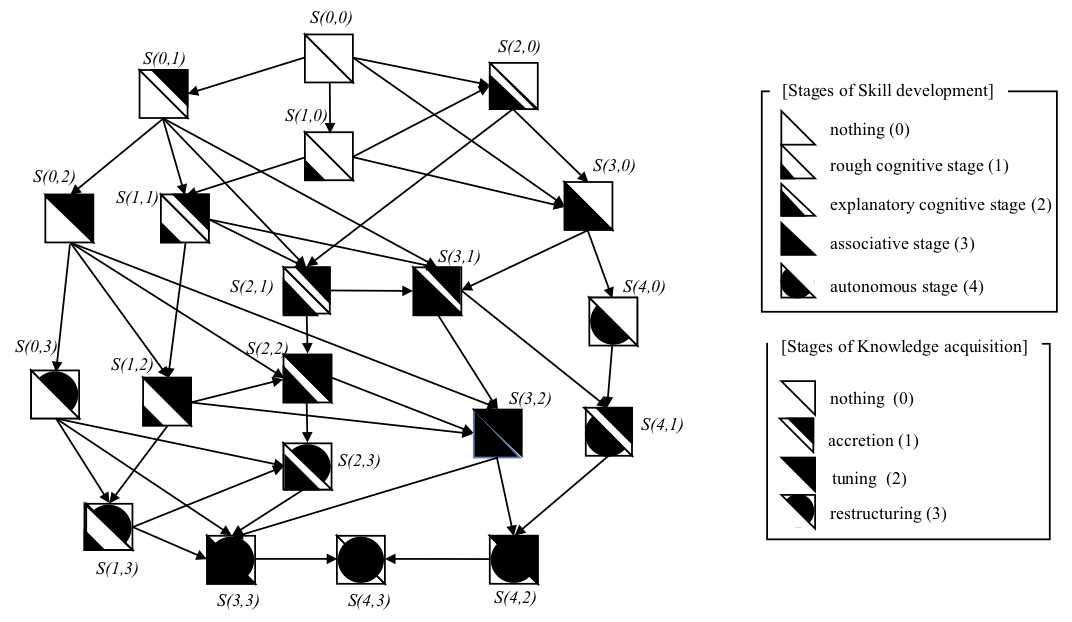
\includegraphics[width=1\textwidth]{images/chap-model-gmif/lgm-model.png}
 \fadaptada{InabaIkedaMizoguchi2003}
\end{figure}

One of the most interesting uses of this model is the representation of transitions in the skill development and knowledge acquisition stages of participants in CL scenarios based on the learning strategies employed by them and the benefits that different learning theories offer. \autoref{fig:lgm-model-cognitiveapprenticeship} shows the representation for the transition of stages in the development of skill and acquisition of knowledge involved in a CL scenario based on the cognitive apprentice theory in which the black arrows imply the application of the learning strategies that facilitates the learner’s growth process.

 \begin{figure}[htb]
 \caption[Transitions in the LGM model for cognitive apprenticeship scenarios]{Transitions in the LGM model for cognitive apprenticeship scenarios. On the left side, stages in the learning by apprentice strategy for participants who play the apprentice role. On the right side, stages in the learning by guiding strategy for participants who play the master role}
 \label{fig:lgm-model-cognitiveapprenticeship}
 \centering
 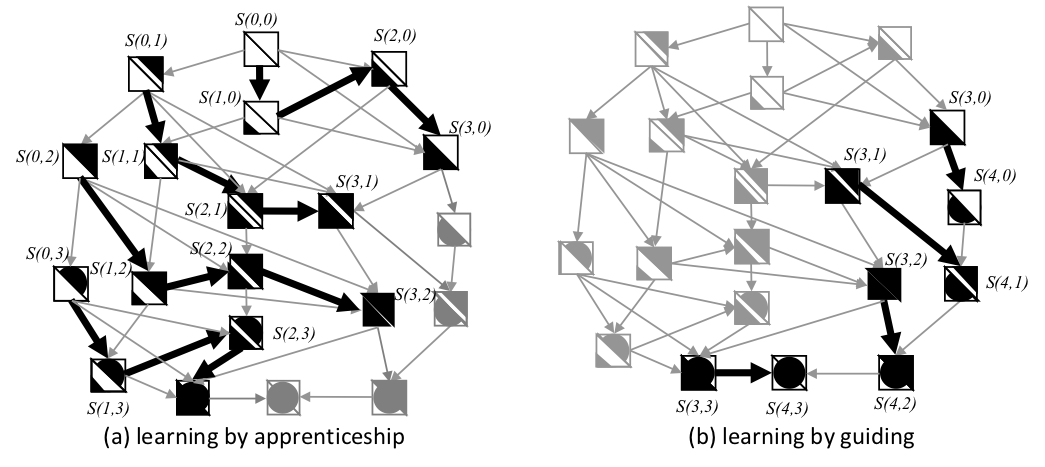
\includegraphics[width=1\textwidth]{images/chap-model-gmif/lgm-model-cognitiveapprenticeship.png}
 \fadaptada{IsotaniMizoguchiInabaIkeda2010}
\end{figure}

On the left side of \autoref{fig:lgm-model-cognitiveapprenticeship} is shown the transition of stages for the apprenticeship learning strategy, where the transition of stages in the LGM model represent the growing in cognitive skills from $s(0,y)$:\emph{nothing} into the $s(3,y)$:\emph{associative stage} through the $s(1,y)$:\emph{rough-cognitive stage} and the $s(2,y)$:\emph{explanatory-cognitive stage}. These transitions in the skill development are transitions carried out by participants who play the apprentice role. On the right side of \autoref{fig:lgm-model-cognitiveapprenticeship} is shown the transitions of stages described by the learning strategy \aspas{\emph{learning by guiding}} in the LGM model. According to this learning strategy, the participant who plays the master role grows in his/her cognitive skill from the $s(3,y)$:\emph{associative stage} into the $s(4,y)$:\emph{autonomous stage}.

With the use of the LGM model, any learning strategy or educational best practice can be explicitly described as a path on the graph, facilitating the understanding, visualization and utilization of the model \cite{IsotaniMizoguchiInabaIkeda2010}.

\subsection{Three-channel Flow Model}
\label{subsec:three-channel-flow-model}

\emph{Csikszentmihalyi’s flow theory} constitutes an important theory regarding to affective states of people during activities that require active work, such as discussions, exercises, and group activities \cite{Csikszentmihalyi2014,SnyderLopezPedrotti2010}. This theory has been applied in several fields, including game design, commerce, and education. The key concept of this theory is the \aspas{\emph{The Zone Flow}} as a situation in which a person is so engaged and focused on a particular task that he/she is completely immersed in it. According to the flow theory, to achieve the flow state, the following conditions must be satisfied:

\begin{itemize}
\item Clear goals in which the expectations and rules are clearly discernable
\item Direct and immediate feedback in which the successes and failures of the tasks are apparent, so that behavior can be adjusted as needed
\item Good balance between the perceived ability and challenge
\end{itemize}

One of the conditions given above is that the flow state only occurs if there is a good balance between the perceived challenges of the task at hand and the learner’s own perceived ability to solve it. This means that the definition of an appropriate challenge (i.e. level of difficulty) is fundamental to design situations that promotes a flow state \cite{LinehanBellordKirmanMorfordRoche2014}. Thus, Csikszentmihalyi proposes the three-channel flow model \cite{Csikszentmihalyi2008} shown in \autoref{fig:three-channel-flow-model}, in which both anxiety and boredom drive persons to frustration. When a task is too difficult to be solved, it causes anxiety because it is perceived as too challenging or because the person’s ability level is not sufficient to solve the task. In the same way, when a task is too easy it causes boredom because it is not challenging enough, or because the person’s ability level is too high for the task.

 \begin{figure}[htb]
 \caption{Affective states in terms of perceived ability level and challenge level, according to the three-channel flow model}
 \label{fig:three-channel-flow-model}
 \centering
 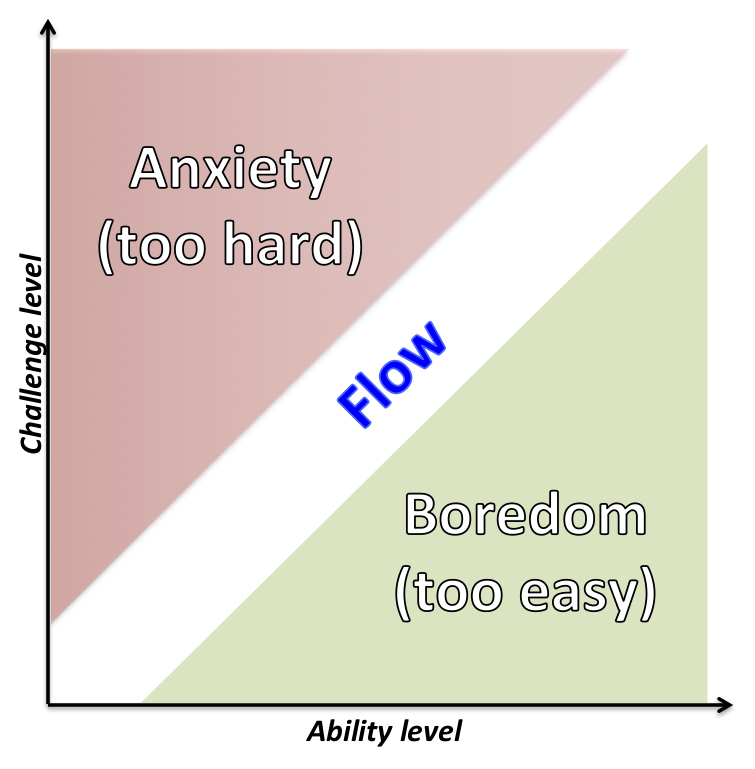
\includegraphics[width=0.5\textwidth]{images/chap-model-gmif/three-channel-flow-model.png}
 \fadaptada{Csikszentmihalyi2008}
\end{figure}

The three-channel flow model has been frequently used to build instruments and tools for the detection of the flow state \cite{KortReillyPicard2001,PearceAinleyHoward2005,Esteban-MillatMartinez-LopezHuertas-GarciaMeseguerRodriguez-Ardura2014a,LeeJhengHsiao2014}. More recently, in the context of computer education and instructional technology, studies have attempted to analyze and modeling the flow state in order: (a) to evaluate the participants’ interactions with learning objects; (b) to personalize educational activities (e.g. lessons); and (c) to develop better learning content. In the context of game-based learning, a framework to support the integration of games as learning activities is proposed by \citeonline{delBlancoTorrenteMarchioriMartinez-OrtizMoreno-GerFernandez-Manjon2012}. To do so, they identified key aspects about the mechanisms that facilitate the use of pedagogical approaches with games to keep students in the flow state. Then, they proposed a workflow to integrate games into the learning process. As a result, this workflow can be used to create guidelines for helping instructional designers the use (and reuse) of games in the learning process. Although this work provides some initial support for creating better learning experiences using game in the learning process, if the games themselves do not have the qualities and attributes necessary to maintain student engagement, the flow experiences will not occur. Considering this problem, \citeonline{KiiliLainemadeFreitasArnab2014} proposed a framework for analyzing and designing educational games based on the flow theory. This framework describes several dimensions of flow experience as well as meaning factors that affect the design of game-based learning activities.

Despite the broad use of the three-channel flow model in educational contexts and its use in game-based learning, to the best of the knowledge for the author of this dissertation, there is not a computational model based on the three-channel flow model that provides support to create CL scenarios that maintain the flow state in the participants while offering theoretical justifications regarding the learner’s growth as an indicator for the perceived ability level.
In particular, there is no computational help to define the appropriate levels of challenges for the game elements of a gamified CL scenario.

\section{Integrating the Learner’s Growth Model and the Three-channel Flow Model}
\label{sec:integrating-learners-growth-model-flow-theory}

The perceived challenge and ability level balance of flow theory can be determined as the current stage of the participant in the LGM model, and the challenge level to maintain the learner in the flow state. Thus, to integrate the representation of the learner’s growth process and the condition of good balance between the perceived challenge and ability, the \emph{Learner’s \textbf{G}rowth \textbf{M}odel \textbf{I}mproved by \textbf{F}low Theory}, hereinafter referred to as GMIF model, has been proposed as a LGM model in which the arrows $s(x_{1},y_{1}) \to s(x_{2},y_{2})$ are labeling with the form $[z_{min}; z_{max}]$ to indicate the \emph{minimum challenge level} ($z_{min}$) and the \emph{maximum challenge level} ($z_{max}$) that are necessary to maintain the learner's flow.

Before to present the algorithm proposed to create a GMIF model with a n-scale of challenge level (\emph{n-scale GMIF model}), a five-scale GMIF model is presented to introduce and detail the elements involved in the building of a GMIF model. After that, the algorithm to create a n-scale GIMF model is presented, and also, the benefits and application of GMIF model in the learning design are detailed.

\subsection{Five-scale GMIF Model}
\label{subsec:five-scale-gmif-model}

In the three-channel flow model (detailed in \autoref{subsec:three-channel-flow-model}), the levels of perceived challenge and ability are used as indicators to identify the current person's affective state in zones of anxiety, flow, and boredom. These two indicators are represented as axes in the three-channel flow model to depict situations where a learner are anxious, bored or in a flow state. These situations could be represented as a rectangular regions in the plane defined by the division of the perceived challenge and ability axes. Thus, to build a GMIF model, two three-channel flow models with the division of $5 \times 5$ rectangular regions are obtained by dividing the axes into five parts. Then, the transitions of the skill development defined by the LGM model are set to the ability axis using a uniform distribution in the first three-channel flow model to define a five-scale three-channel flow model of skill development stages and challenge levels. In the second three-channel flow model, the transitions of the knowledge acquisition defined by the LGM model are set to the ability axis using also a uniform distribution to define a five-scale three-channel flow model of knowledge acquisition stages and challenge levels.

\begin{figure}[htb]
 \caption{Five-scale three-channel flow model of skill development}
 \label{fig:five-scale-three-channel-flow-model-skill-development}
 \centering
 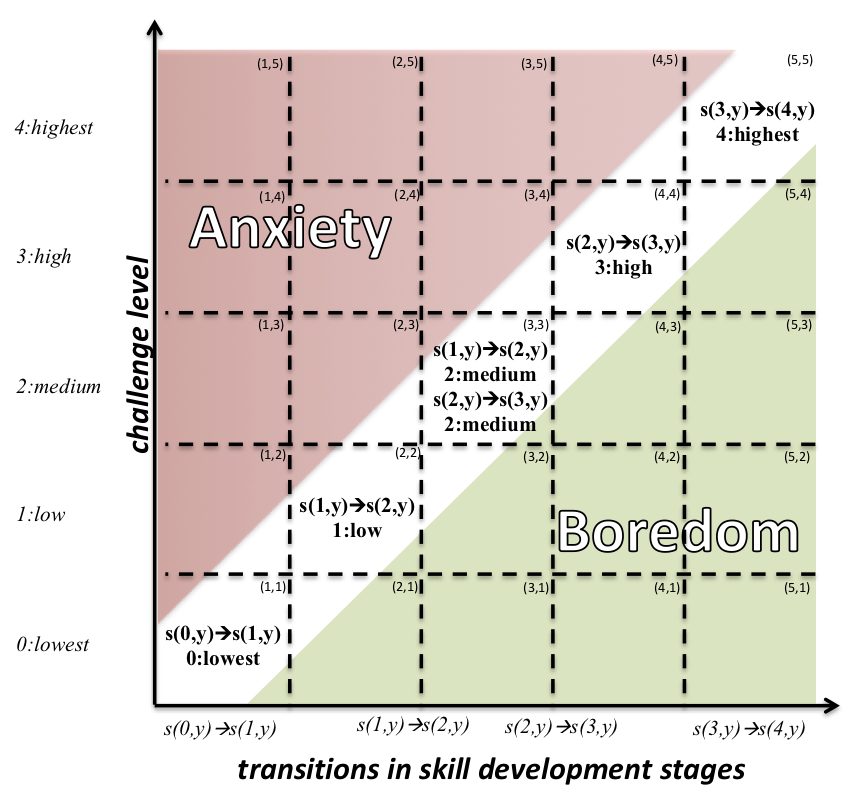
\includegraphics[width=0.65\textwidth]{images/chap-model-gmif/five-scale-three-channel-flow-model-skill-development.png}
 \fautor
\end{figure}

\autoref{fig:five-scale-three-channel-flow-model-skill-development} shows the five-scale three-channel flow model of skill development stages and challenge levels. In this model, the five-scale challenge levels are: 0:\emph{lowest}, 1:\emph{low}, 2:\emph{medium}, 3:\emph{high}, 4:\emph{highest}. The transitions in the skill development are: $s(0,y) \to s(1,y)$: from \emph{nothing} to \emph{rough-cognitive stage}; $s(1,y) \to s(2,y)$: from \emph{rough-cognitive stage} to \emph{explanatory-cognitive stage}; $s(2,y) \to s(3,y)$: from \emph{explanatory-cognitive stage} to \emph{associative stage}; $s(3,y) \to s(4,y)$: from \emph{associative stage} to \emph{autonomous stage}. According to this model, the label sequence of minimum and maximum challenge levels for maintaining the learner’s flow is $s_{1}=\{[0;0], [1;2], [2;3], [4;4]\}$ in which the first element \aspas{$[0;0]$} extracted from region $(1,1)$ means that, during the transition: $s(0,y) \to s(1,y)$, the proper level of challenge to maintain the learner’s flow is 0:\emph{lowest}. The second element \aspas{$[1;2]$} extracted from regions $(2,2)$ and $(3,3)$ means that, during the transition $s(1,y) \to s(2,y)$, the proper level of challenge to maintain the learner’s flow is in the range of 1:\emph{low} to 2:\emph{medium}. The third element \aspas{$[2;3]$} means that, during the transition $s(2,y) \to s(3,y)$ extracted from region $(3,3)$ and $(4,4)$, the proper level of challenge to maintain the learner’s flow is in the range of 2:\emph{medium} to 3:\emph{high}. Finally, the fourth element \aspas{$[4;4]$} extracted from region $(5,5)$ means that, during the transition $s(3,y) \to s(4,y)$, the proper level of challenge is 4:\emph{highest}.
 
By employing the transitions $s(x,0) \to s(x,1) \to s(x,2) \to s(x,3)$ of knowledge acquisition ($s(x,0) \to s(x,1)$: from \emph{nothing} to \emph{accretion stage}; $s(x,1) \to s(x,2)$: from the \emph{accretion stage} to \emph{tuning stage}; $s(x,2) \to s(x,3)$: from the \emph{tuning stage} to \emph{restructuring stage}), the five-scale three-channel flow model shown in \autoref{fig:five-scale-three-channel-flow-model-knowledge-acquistion} has been obtained to represent the relation of knowledge acquisition stages and challenge levels. In this space, labels of minimum and maximum challenge levels for maintaining the learner’s flow is defined by the sequence $s_{2} = \{[0;0], [1;3], [4;4]\}$ in which the first element \aspas{$[0;0]$} extracted from the region $(1,1)$ means that means that, during the transition $s(x,0) \to s(x,1)$, the level of challenge should be 0:\emph{lowest} to maintain the learner’s flow. The second element \aspas{$[1;3]$} extracted from regions $(1,1)$, $(2,2)$ and $(3,3)$ means that, during the transition $s(x,1) \to s(x,2)$, the proper level of challenge to maintain the learner’s flow is in the range of challenge levels 1:\emph{low}, 2:\emph{medium} and 3:\emph{high}. Finally, the proper level of challenge during the transition $s(x,2) \to s(x,3)$ is 4:\emph{highest}.

 \begin{figure}[htb]
 \caption{Five-scale three-channel flow model of knowledge acquisition}
 \label{fig:five-scale-three-channel-flow-model-knowledge-acquistion}
 \centering
 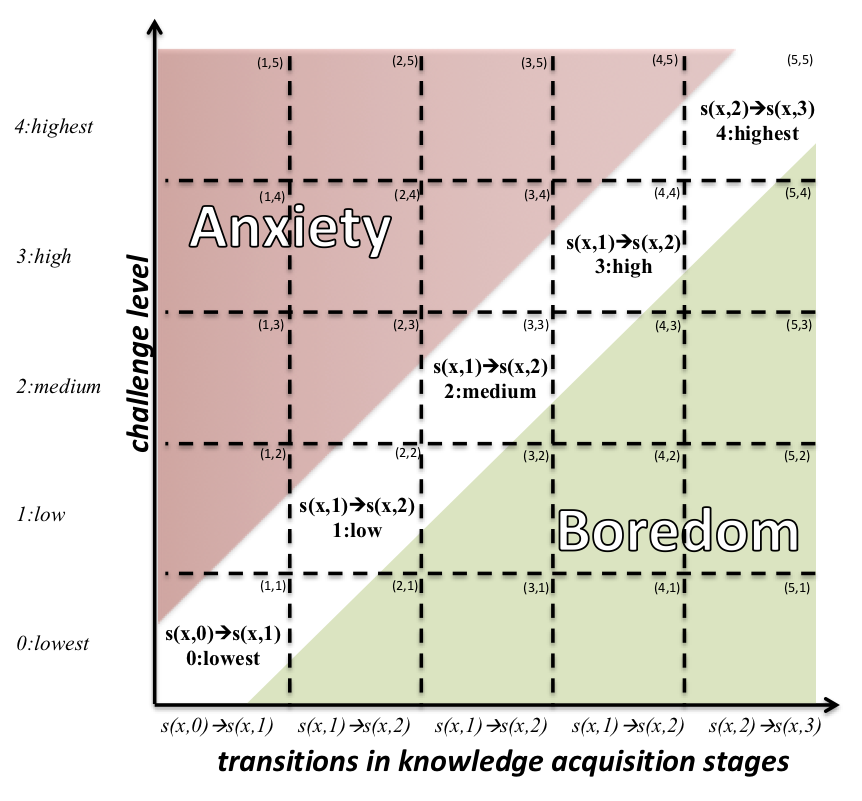
\includegraphics[width=0.65\textwidth]{images/chap-model-gmif/five-scale-three-channel-flow-model-knowledge-acquistion.png}
 \fautor
\end{figure}

To obtain the five-scale GMIF model, the relationship between the transitions of stages in the skill development and knowledge acquisition and the challenge levels should be clearly understood from the two five-scale three-channel flow models shown in \autoref{fig:five-scale-three-channel-flow-model-skill-development} and \autoref{fig:five-scale-three-channel-flow-model-knowledge-acquistion}. With this knowledge, it is possible to design CL scenarios that (i) favor the maintenance of a flow state for students; and (ii) help them to achieve desired educational goals (i.e. acquisition of knowledge or development of skills). To accomplish these objectives, the label sequences ($s_{1}$ and $s_{2}$) to maintain the learner's flow identified from \autoref{fig:five-scale-three-channel-flow-model-skill-development} and \autoref{fig:five-scale-three-channel-flow-model-knowledge-acquistion}, which enables us to understand when a participant are in flow state (by making the correlation between knowledge and skills with a five-scale of challenge level), to adequately label each transition (i.e. $s(x,y) \to s(x',y')$) between states in the LGM with a tuple \aspas{$[z_{min}; z_{max}]$,} where $z_{min}$ refers to the minimum challenge level necessary of to be considered interesting and not too easy, and $z_{max}$ refers to the maximum challenge level possible to be considered challenging but not too difficult.

To define the values of $z_{min}$ and $z_{max}$ in the labels \aspas{$[z_{min}; z_{max}]$} of a transition $s(x,y) \to s(x',y')$, the sequences $s_{1}$ and $s_{2}$ are used to define the proper levels of challenge for the transitions related to skill development and knowledge acquisition, respectively. Thus, when a transition $s(x, y) \to s(x', y)$ is related to the skill development, the sequence $s_{1}$ extracted from the model shown in \autoref{fig:five-scale-three-channel-flow-model-skill-development} is used to label this transition. For example, to develop skill from the \emph{explanatory-cognitive stage} to the \emph{associate stage}, the transition $s(2,y) \to s(3,y)$ is labeled in the LGM graph as $[2;3]$ by looking at where this transition is located in the flow area of \autoref{fig:five-scale-three-channel-flow-model-skill-development}. In this particular situation, the label $[2;3]$ means that, to maintain the learner’s flow, the level of challenge for an element in the learning scenario should be selected in the range of 2:\emph{medium} to 3:\emph{high}. Following the same procedure, the transitions related to knowledge acquisition are used to label the transitions $s(x,y) \to s(x,y')$ defined by the sequence $s_{2}$.

\autoref{fig:five-scale-gmif-model} shows the five-scale GMIF model that results from labeling the LGM with a scale of five levels of challenge. 

 \begin{figure}[htb]
 \caption{Five-scale learner's growth model improved by the flow theory}
 \label{fig:five-scale-gmif-model}
 \centering
 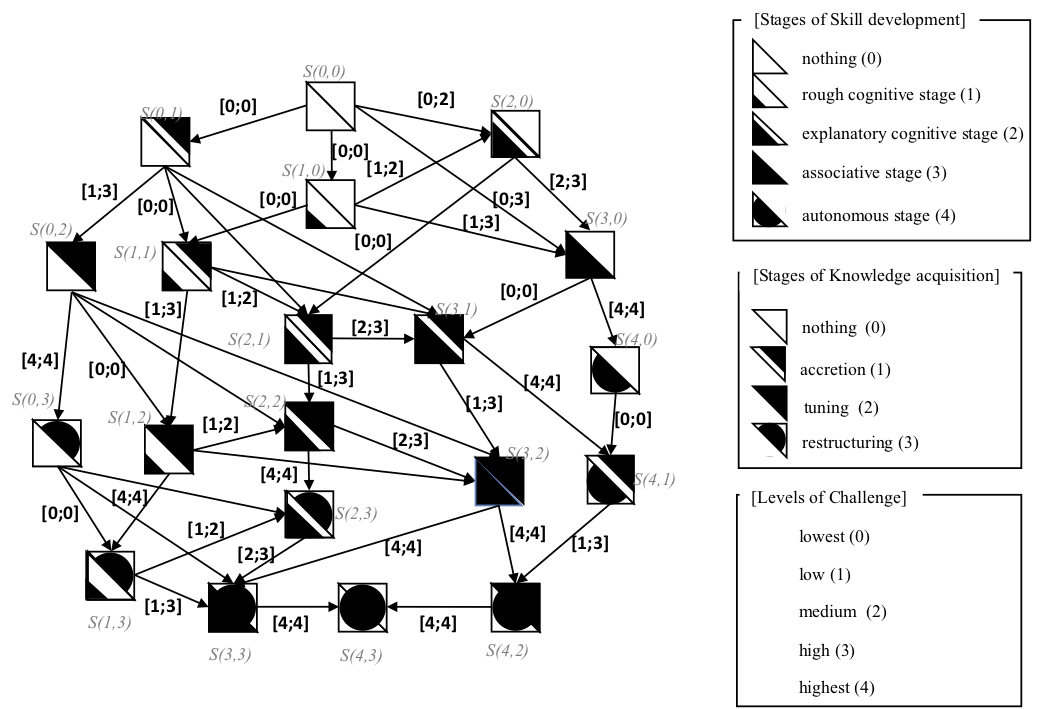
\includegraphics[width=1\textwidth]{images/chap-model-gmif/five-scale-gmif-model.png}
 \fautor
\end{figure}

\newpage
\subsection{Algorithm for Building a n-scale GMIF Model}
\label{subsec:pseudo-algorithm-n-scale-gmifs}

\autoref{algorithm:build-n-gimf-model} shows the algorithm proposed to build a GMIF model with a n-scale of challenge levels (\emph{n-scale GMIF model}), where the expected difference for the levels of challenge in the flow area is passed as the param \aspas{\emph{delta}} (as a second argument that has the default value zero). In the algorithm, the variable GMIF contains the labels for the transitions $t = s(x,y) \to s(x’,y’)$ of the LGM model, and each label is represented as the form $[z_{min}; z_{max}]$, which indicates the minimum $z_{min}$ and maximum $z_{max}$ levels of challenge that is necessary to maintain a participant is the flow state.

In the algorithm, the flow regions for the \aspas{\emph{transitions in skill development stages} vs \emph{challenge level}} and the \aspas{\emph{transitions in knowledge development stages} vs \emph{challenge level}} are obtained by the function \aspas{\emph{get\_flow\_region}} (lines 2-3), where the first parameter is the number of transitions for skill development or knowledge acquisition, and the second parameter is the n-scale of space for the challenge level, and the third parameter is the expected difference for levels of challenge.

\begin{algoritmo}
\caption{Algorithm to build a $n$-scale GMIF model}
\label{algorithm:build-n-gimf-model}
\begin{algorithmic}[1]\small
\Procedure{build\_GIMF}{n\_scale = 5, delta = 0}
  \State skill\_flow $\gets$ get\_flow\_region(4, n\_scale, delta)
  \State knowledge\_flow $\gets$ get\_flow\_region(3, n\_scale, delta)
  \ForAll{$t = (x,y) \to (x',y)$ in LGM model}
    \State GIMF[t] $\gets$ $\cup_{i=x}^{x'-1}$skill\_flow[i]
  \EndFor
  \ForAll{$t = (x,y) \to (x,y')$ in LGM model}
    \State GIMF[t] $\gets$  knowledge\_flow[y]
  \EndFor
\EndProcedure
\end{algorithmic}
\end{algoritmo}

Because the transition in the skill development stages includes flexibility that allows to increase the skill stage without following all the transitions between stages, transitions $s(x,y) \to s(x',y)$ are labeled in all levels of challenge that are defined in intermediate transitions as shown in the lines (4-6) of \autoref{algorithm:build-n-gimf-model}. For example, it is possible to go from 0:\emph{nothing} to 3:\emph{associative stage} without moving through the intermediate stages 1:\emph{rough-cognitive stage} and 2:\emph{explanatory-cognitive stage}; thus, the transition $s(0,y) \to s(3,y)$ is labeled with the union of challenge levels defined in the transitions $s(0,y) \to s(1,y)$, $s(1,y) \to s(2,y)$ and $s(2,y) \to s(3,y)$. In the case of transitions related to the knowledge acquisition, the transition of stages is completed step-by-step without skipping any of the stages; thus, the transition $s(x,y) \to s(x,y')$ is labeled by setting the corresponding levels of challenge for the transitions of knowledge acquisition at shown in lines (7-9) of \autoref{algorithm:build-n-gimf-model}.

\autoref{algorithm:get-flow-region} details the algorithm for the function \aspas{\emph{get\_flow\_region}.} This function calculates the flow region in the n-scale three-channel flow models, where the flow region is represented as an array of size $m$ (number of transitions for skill development or for knowledge acquisition) in which each $i$-th element contains the levels of challenge for the transition from the $i$-th stage to the next stage ($i+1$ stage). For an instance of five levels of challenge and three transitions of knowledge acquisition (shown in \autoref{fig:five-scale-three-channel-flow-model-knowledge-acquistion}), the flow region as a result of the algorithm is a sequence $s = \{[0;0], [1;3], [4;4]\}$, where the first element \aspas{$[0;0]$} indicates the level of challenge as 0:\emph{lowest} for the transition $s(x,0) \to s(x,1)$.

\begin{algoritmo}
\caption{Algorithm to obtain a flow region in $m$ transitions with $n$ challenges}
\label{algorithm:get-flow-region}
\begin{algorithmic}[1]\small
\Function{get\_flow\_region}{$m$, $n\_challenges = 5$, $delta = 0$}
  \State $n \gets n\_challenges$%\LeftComment{normalize the number of challenge levels}
  \If{($n\_challenges > m$) and is.odd($n\_challenges$)}
    \State $n \gets n-1$
  \EndIf
  \State $distr \gets$ initialize\_array($m$, $\lfloor s/m \rfloor$)%\LeftComment{sets number of challenge levels for each transition}
  \State $rest \gets s - m \lfloor s/m \rfloor$
  \If{($rest > 0$)}
    \State $inv\_sigma \gets (n-rest)/2$
    \For{$i \gets 0$ to $rest-1$}
      \State $distr[inv\_sigma+i] \gets distr[inv\_sigma+i]+1$
    \EndFor
  \EndIf
  \State $flow[0].min \gets 0$%\LeftComment{make labels for flow region}
  \State $flow[0].max \gets distr[0] - 1$
  \For{$i \gets 1$ to $m-1$}
    \State $flow[i].min \gets flow[i-1].max + 1$
    \State $flow[i].max \gets flow[i-1].max + distr[i]$
    \If{($n\_challenges > m$) and is.odd($n\_challenges$)}
      \If{is.odd($m$) and ($i = \lfloor m/2 \rfloor$)}
        \State $flow[i].max \gets flow[i].max + 1$
      \EndIf
      \If{is.even($m$)}
        \If{$i = \lfloor m/2 \rfloor - 1$}
          \State $flow[i].max \gets flow[i] + 1$
        \EndIf
        \If{$i = \lfloor m/2 \rfloor$}
          \State $flow[i].min \gets flow[i] - 1$
        \EndIf
      \EndIf
  \EndIf
  \EndFor
  \ForAll{$r$ in $flow$}
    \If{($r.max = -1$)}
      \State $r.min \gets -1$
    \Else
      \State $r.min \gets r.min - delta$
      \State $r.max \gets r.max + delta$
    \EndIf
  \EndFor
  \State \Return $flow$
\EndFunction
\end{algorithmic}
\end{algoritmo}

The function \aspas{\emph{get\_flow\_region}} described as the \autoref{algorithm:get-flow-region} is summarized in a narrative form as:
Calculates the number of levels that should be distributed for each transition of stage (lines 2-13). These values are calculated through a uniform distribution that tries to maintain the same number of levels in all stages. The stages located in the same distance of the mean stage should have the same number of levels. For example, the distribution of eight levels of challenge in five transitions is defined as the array $s = \{1,2,2,2,1\}$, where the second, third, and fourth transitions are set with two levels, it is $s(1) = s(2) = s(3) = 2$, whereas the first and fifth transitions are set with one level, it is $s(0) = s(4) = 1$. Finally, the transition located in the third transition is set with two levels, it is $s(2) = 2$. The steps that calculate these levels are as follows:

\begin{itemize}
\item
The normalization for the number of challenges. This is done to avoid the non-uniform distribution that happens when this number is odd and it is greater than the number of transitions. For example, the distribution of nine levels among four transitions only can be done by setting one transition with three levels, and setting the rest of transitions with two levels. Therefore, the normalization for the levels of challenge is done by reducing the number of levels by one (lines 2-5). In the previous example, the distribution of nine levels into four transitions can be defined as the array $s = \{2, 2, 3, 2\}$ before the normalization, and the distribution of these nine levels after the normalization is defined as the array $s = \{2, 2, 2, 2\}$.
\item
After the normalization, the minimum number of challenge level for each stage is defined by the function \aspas{\emph{initialize\_array}} (line 6), which initializes an array of size $m$ with the value. The remaining levels of challenge (line 7) are distributed according to the position \aspas{$inv\_sigma$} (lines 10-12). The value \aspas{$inv\_sigma$} is the result of dividing the number of free spaces after the distribution of the remaining challenge levels by two (line 11).
\end{itemize}

After determining the number of challenge levels that will be distributed for each transition (\emph{distr}), the next step is to set the labels for the flow region that has no expected difference in the levels of challenge (lines 14-32). Thus, the process to define these labels consists in:

\begin{itemize}
\item To set the flow region for the first transition through the definition of the minimum challenge level with value zero (line 14), and the definition of the maximum challenge level with the number of challenge levels decreased by one (line 15).
\item Setting the flow region for the rest of the transitions (lines 16-32). The minimum level of challenge is defined as the maximum challenge level of the previous transition increased by one (line 17), and the maximum challenge level is defined as the maximum challenge level of the previous transition increased by the number of challenge levels (line 18). For cases in which the normalization of levels has been done, the following two rules must be applied:

\begin{itemize}
\item If the number of transitions is odd, then the maximum challenge level is increased by one in the mid-transition (lines 20-22). Thus, the flow region for nine levels of challenge in five transitions is defined as the array $s = \{[0;0], [1;2], [3;5], [6;7], [8;8]\}$.
\item If the number of transitions is even, then there are two mid-transitions: the first mid-transition is located in the position $\lfloor m/2 \rfloor - 1$, and the second mid-transition is located in the position $\lfloor m/2 \rfloor$. Next, the maximum challenge level is increased by one in the first mid-transition (lines 24-26). Finally, the minimum challenge level is decreased by one for the second mid-transition (lines 27-29). Thus, the flow region for nine challenge levels in four transitions is defined as the array $s = \{[0;1], [2;4], [4;6], [7;8]\}$.
\end{itemize}
\end{itemize}

Finally, the expected difference in level of challenge, defined as the parameter delta, is used to decrease and increase the minimum and maximum levels of challenge for each transition in the flow region (lines 33-40).

\subsection{Benefits and Application of GMIF Model}

Several factors must be considered during the learning design process, such as learning goals, pedagogical preferences, intervention timing, type of feedback, students’ needs, available resources, and so on. The work of \citeonline{KoedingerBoothKlahr2013} estimates that there is a poll of 330 (205 trillion) instructional choices that could be considered when designing a learning activity. Unfortunately, most designers and educators do not have enough knowledge/skills to cope with this huge number of instructional choices and select those choices that are the best fit for a particular situation. To provide help for the instructional designers in this process, the n-scale GMIF model provides an appropriate integration of instructional design with learning theories, models of learner’s growth, and the three-channel flow model, in order to reduce the complexity of the learning design task. Specifically, the GIMF model can be used to foster flow experiences in theory-based learning scenarios.

\subsubsection*{Foster Flow Experiences in Theory-Based Learning Scenarios}

To get students into the flow state and produce optimal learning experiences, one should initially consider: 

\begin{itemize}
\item The student's initial stage and learning objectives (as final stage) in terms of knowledge acquisition and skills development \cite{Anderson1982,RumelhartNorman1976};
\item The learning path to be follow by the student based on theoretical justifications \cite{IsotaniMizoguchiInabaIkeda2010,Romiszowski1981}; and 
\item The definition of the challenge level based on the three-channel flow model. Here it is necessary to select the necessary challenge level to keep the student in the flow state \cite{Csikszentmihalyi2014,DMello2012}. 
\end{itemize}

The GMIF model has been developed to support these steps. In the first step, the GMIF model provides a standard to describe and represent learning objectives as well as the learner’s stage. Thus, the problem of sharing learning designs among people and computers is reduced. Accordingly, an instructional designer can indicate the initial stage of the student and select his/her learning objectives. Both correspond to stages in the GMIF model. After that, the designer can check manually or automatically (using learning design authoring tools) which learning strategy based on instructional/learning theories provides an adequate learning path that supports a learner in achieving the desired goals. In this situation, the GMIF model offers a visual representation as a sequence of arrows on the GMIF model that represent learning strategies and how they support the learner’s growth process. Finally, to provide a flow experiences, the designer needs to define the level of challenge that is needed to maintain the student in the flow state. In this regard, the GMIF model will indicate the level of challenge that should be considered when creating tasks to alter the state of the student while keeping him/her motivated.

%%%%%%%%%%%%%%%%%%%%%%%%%%%%%%%%%%%%%%%%%%%%%%%%%%
\section[Application of GIMF Model for the Definition of Game Rewards]{Application of GIMF Model for the Definition of Game Rewards in Gamified CL Scenarios}
\label{sec:application-giving-rewards-by-gimf-model}

With the GMIF model detailed above, we can develop different functions in authoring tools of learning scenarios. A useful function developed by the author of this dissertation is the searching of proper learning objects that will favor and maintain the learner’s flow in the learning scenario \cite{ChallcoAndradeBorgesBittencourtIsotani2016}. Thus, in this function, an instructional designer firstly set the initial and goal stages of a student in a learning scenario using the graphical representation of the GMIF model. Next, each label for a difficulty level in the transition from the initial stage to the goal stage is used as a constraint to search learning objects from different repositories. 

To demonstrate the usefulness of the GIMF model in the gamification of CL scenarios, the definition of game rewards to be promised and given by game agents in gamified instructional and learning events is presented here as an application in which ontological structures to represent gamified I\_L events are used as information source. For accomplish this task, the instructional designer first set the initial and goal stages in the graphical representation of GIMF model using the information provided by the individual goal (\emph{I-goal}) in the instructional and learning event. Then, the learning path from the initial stage to the goal stage is identified as the learning strategy employed by the participant, and the labels of challenge levels are calculated for the arrows in the learning path according to the number of challenges/levels that could have a game component. Finally, these labels can be used as constraints to set the game reward to be promised or given by the game agent to keep the participant in the flow state.

\begin{figure}[htb]
 \caption{Application of the GMIF model to set the game points to be given in the gamified instructional event \aspas{\emph{Gamified Checking}} of the \emph{Gamified Cognitive Apprenticeship Scenario for Master/Yee Achiever and Apprentice/Yee Achiever}}
 \label{fig:set-game-reward-gamified-checking}
 \centering
 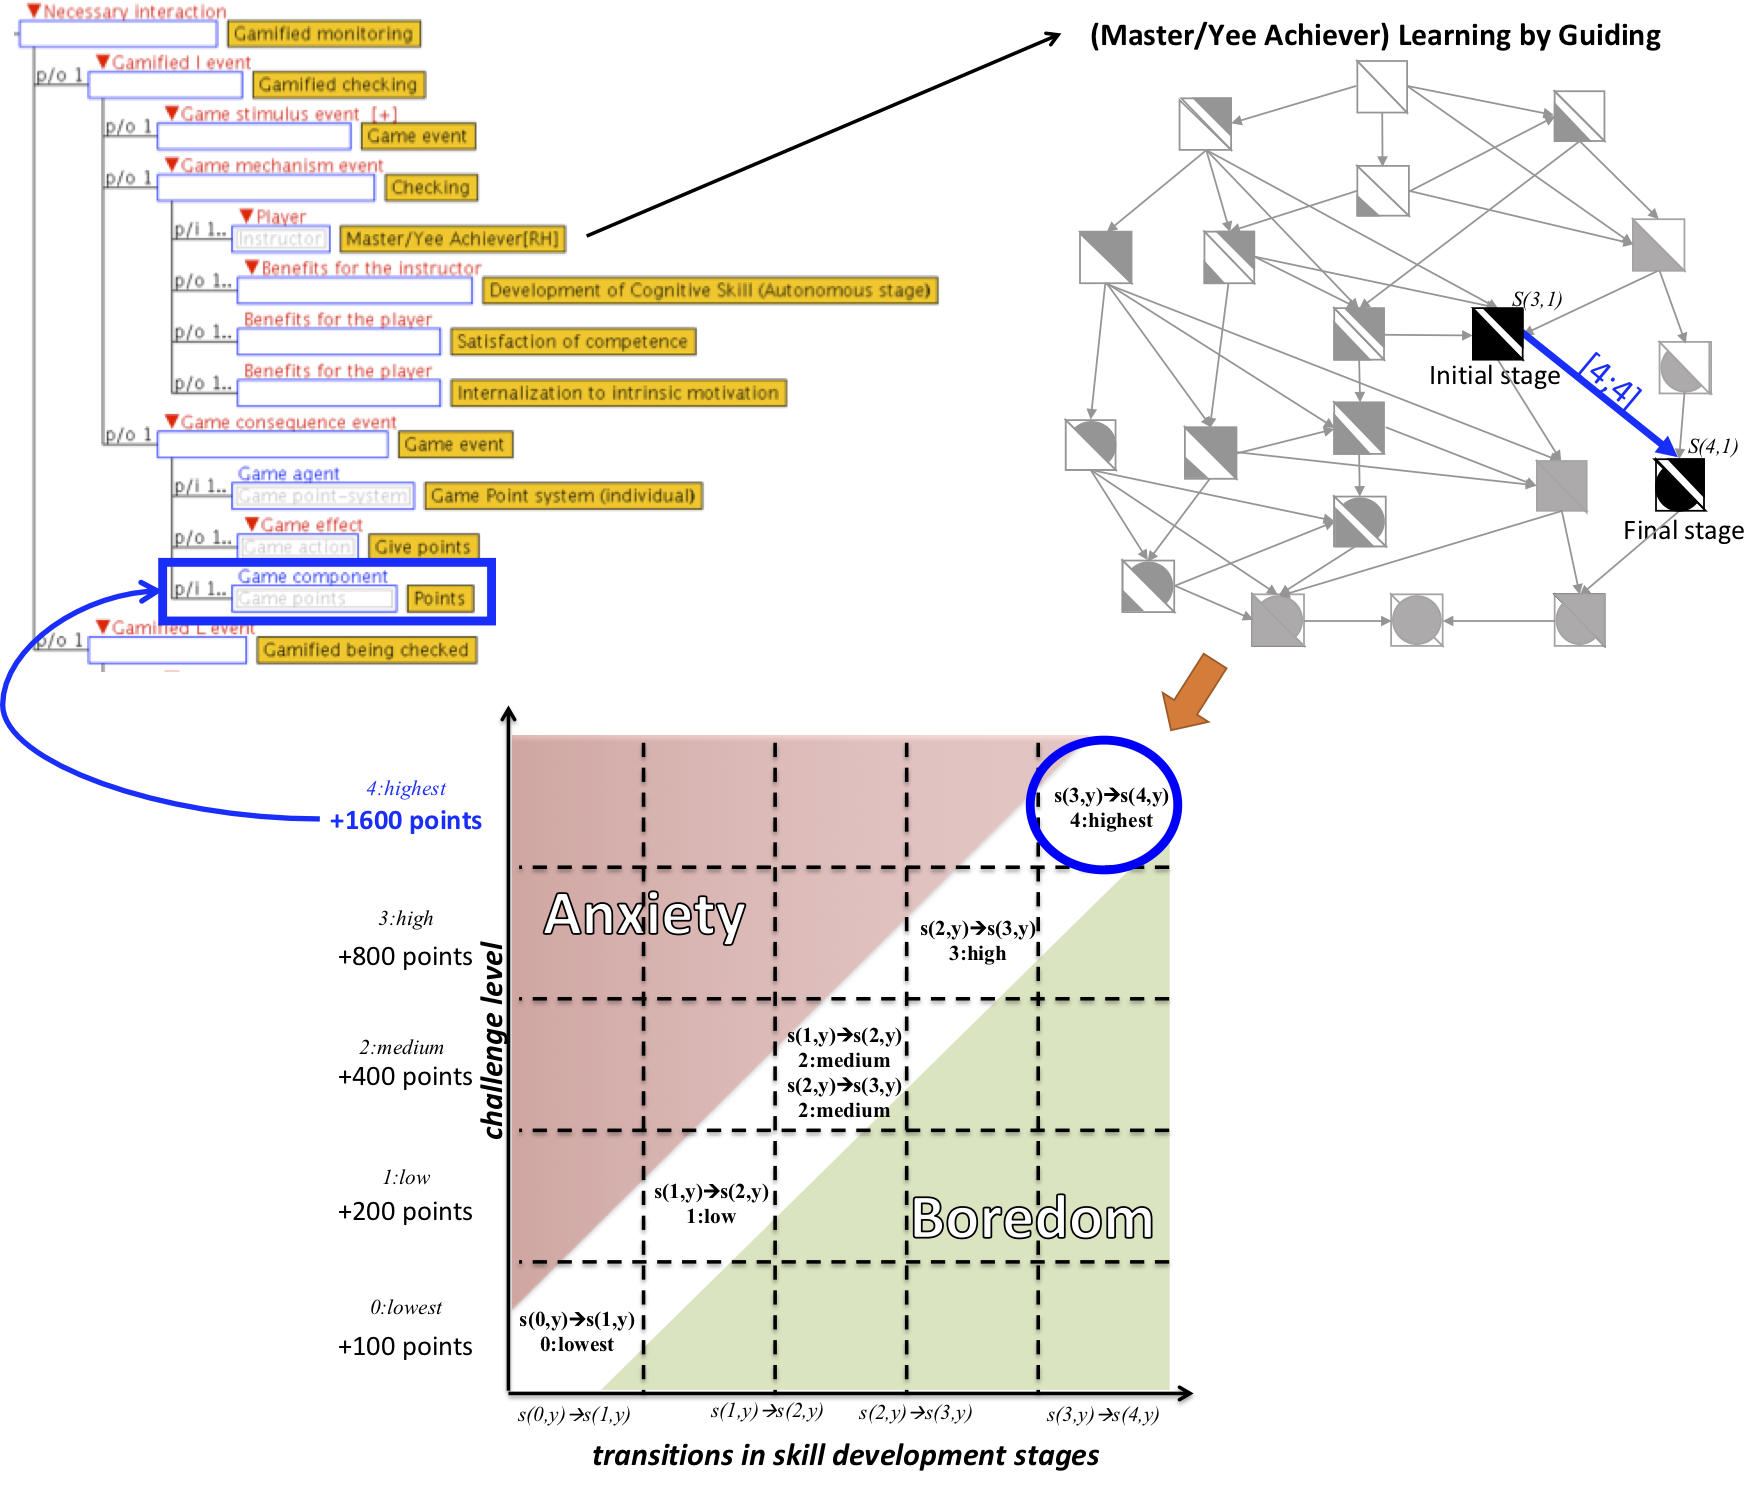
\includegraphics[width=1\textwidth]{images/chap-model-gmif/set-game-reward-gamified-checking.png}
 \fautor
\end{figure}

For the instance shown in \autoref{fig:set-game-reward-gamified-checking}, where the five-scale GMIF model has been applied to set the game points to be given by the point system as consequence of instructional event \aspas{\emph{Checking}} in a gamified CL scenario based on the cognitive apprenticeship theory with the Yee's achiever player role assigned for the master and apprentice role holder - \emph{Gamified Cognitive Apprenticeship Scenario for Master/Yee Achiever and Apprentice/Yee Achiever}. In this situation, the instructional designer set the initial stage for the \emph{Master/Yee Achiever} role holder as $s(3,1)$ - associative stage for skill development and accretion for knowledge acquisition - and the goal stage as $s(4,1)$ - autonomous stage for skill development and accretion for knowledge acquisition. Thus, the learning path in the GIMF model is defined by the learning strategy \aspas{\emph{Learning by Guiding},} and the proper level of challenges that will favor and maintain the \emph{Master/Yee Achiever} in the flow state is defined by the label \aspas{$[4;4]$} that indicate a 4:\emph{highest} challenge level in the five-scale three-channel flow model of skill development stages. Having this flow region, the proper reward to be given in the \emph{Game consequence event} by \emph{Game Point system (individual)} for the \emph{Master/Yee Achiever} role holder is \emph{+1600 points} (as \emph{Game component}).

\begin{figure}[htb]
 \caption{Application of the GMIF model to set the game points to be given in the gamified learning event \aspas{\emph{Gamified Being Checked}} of the \emph{Gamified Cognitive Apprenticeship Scenario for Master/Yee Achiever and Apprentice/Yee Achiever}}
 \label{fig:set-game-reward-gamified-being-checked}
 \centering
 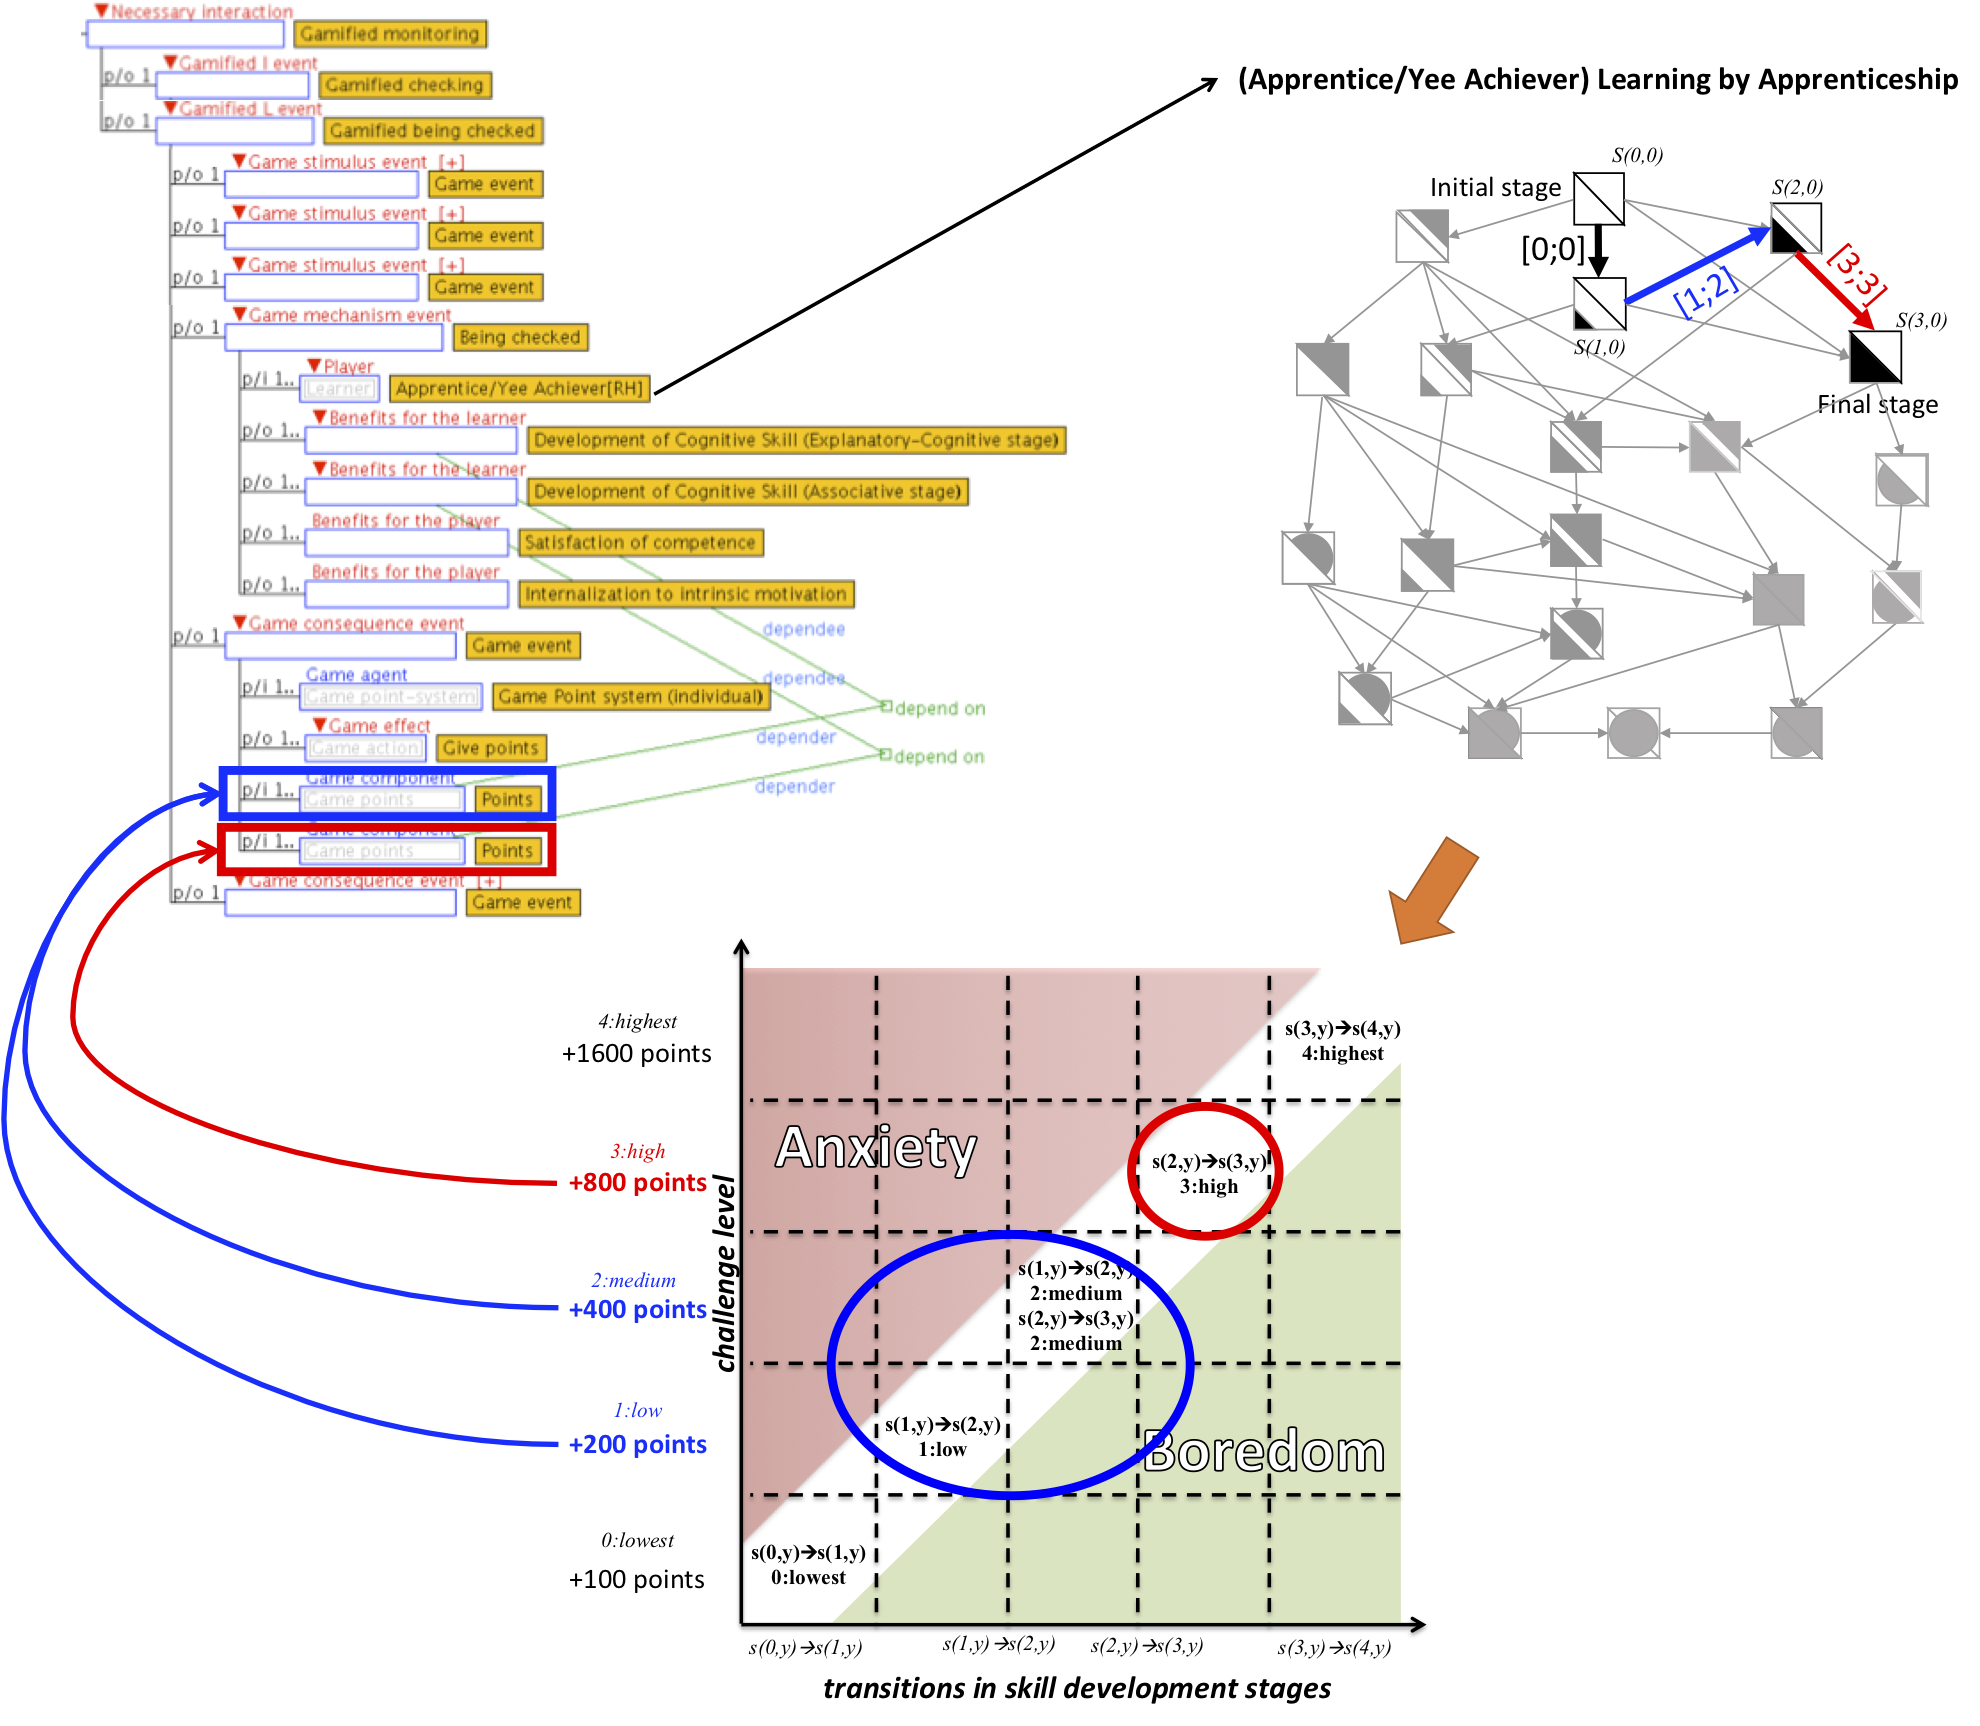
\includegraphics[width=1\textwidth]{images/chap-model-gmif/set-game-reward-gamified-being-checked.png}
 \fautor
\end{figure}

\autoref{fig:set-game-reward-gamified-being-checked} shows the application of GMIF model to set the game rewards in the gamified learning event \aspas{\emph{Gamified Being Checked}.} In this example, the learning path identified for the \emph{Apprentice/Yee Achiever} from the initial stage $s(0,0)$ - nothing for skill development and knowledge acquisition -  to the goal stage $s(3,0)$ - associative stage for skill development and nothing for knowledge acquisition - is based on the learning strategy \aspas{\emph{Learning by Apprenticeship}.} By the application of five-scale GMIF model, the label 
\aspas{$[1;2]$} in the transition $s(1,0) \to s(2,0)$ indicates that the proper challenges levels of 1:\emph{low} and 2:\emph{easy} are necessary to maintain the \emph{Apprentice/Yee Achiever} role holder in the flow state. These challenge levels in the five-scale three-channel flow model of skill development stages correspond to the rewards of \emph{+200 points} or \emph{+400 points} as the game rewards that will be given by the point-system in the game consequence event when the expected benefit for the \emph{Apprentice/Yee Achiver} role holder is the \emph{Development of Cognitive Skill (Exploratory-Cognitive stage)}. The label \aspas{$[3;3]$} in the transition $s(2,0) \to s(3,0)$ of GIMF model indicates that the challenge level to maintain the learner's flow state is 4:\emph{high}. This challenge level corresponds to the game reward \aspas{\emph{+800 points}} as the reward to be given by the point-system to maintain him/her in the flow state during the game consequence event when the expected benefit for the \emph{Apprentice/Yee Achiever} role holder is the \emph{Development of Cognitive Skill (Associative stage)}.

%%%%%%%%%%%%%%%%%%%%%%%%%%%%%%%%%%%%%%%%%%%%%%%%%%
\section{Concluding Remarks}
\label{sec:model-gmif-concluding-remarks} 

Balancing the challenge level of elements in learning scenarios according to the current learner's ability favors the learner's flow state in those scenario. This balancing incorporates the flow theory in the instructional/learning design process by means of a theory-based model that integrates the learner's growth process and the three-channel flow model. This new model, called GMIF model (\emph{Learner's \textbf{G}rowth \textbf{M}odel \textbf{I}mproved by \textbf{F}low Theory}), has been developed by labeling the LGM model (\emph{\textbf{L}earner's \textbf{G}rowth \textbf{M}odel}) with intervals that indicate the proper challenge levels to maintain the learner's flow state in the learning scenario.

An algorithm for labeling the LGM model with a n-scale of challenge levels, and then obtains the n-scale GMIF model, has also been proposed in this chapter. To demonstrate the usefulness of the n-scale GIMF model, an application to set the proper level of game rewards in gamified CL scenarios has been presented. This application has been illustrated providing support to define the points given by a point-system as game consequence events in gamified instructional and learning events. This algorithm and the n-scale GIMF model can be used in computer-based mechanisms and procedures to support the gamification of CL scenarios that favor the learner's flow. Furthermore, empirical studies were conducted to validate the application of GIMF model in the evaluation of the ontological engineering approach to gamify CL scenarios.


\chapter[Computer-based Mechanisms and Procedures to Gamify CL Scenarios]{Computer-based Mechanisms and Procedures to Gamify Collaborative Learning Scenarios}
\label{chapter:computer-based-mechanisms-procedures}

\begin{figure}[htb]
 \caption{Conceptual flow to gamify CL scenarios}
 \label{fig:conceptual-flow-gamify-cl-scenarios}
 \centering
% 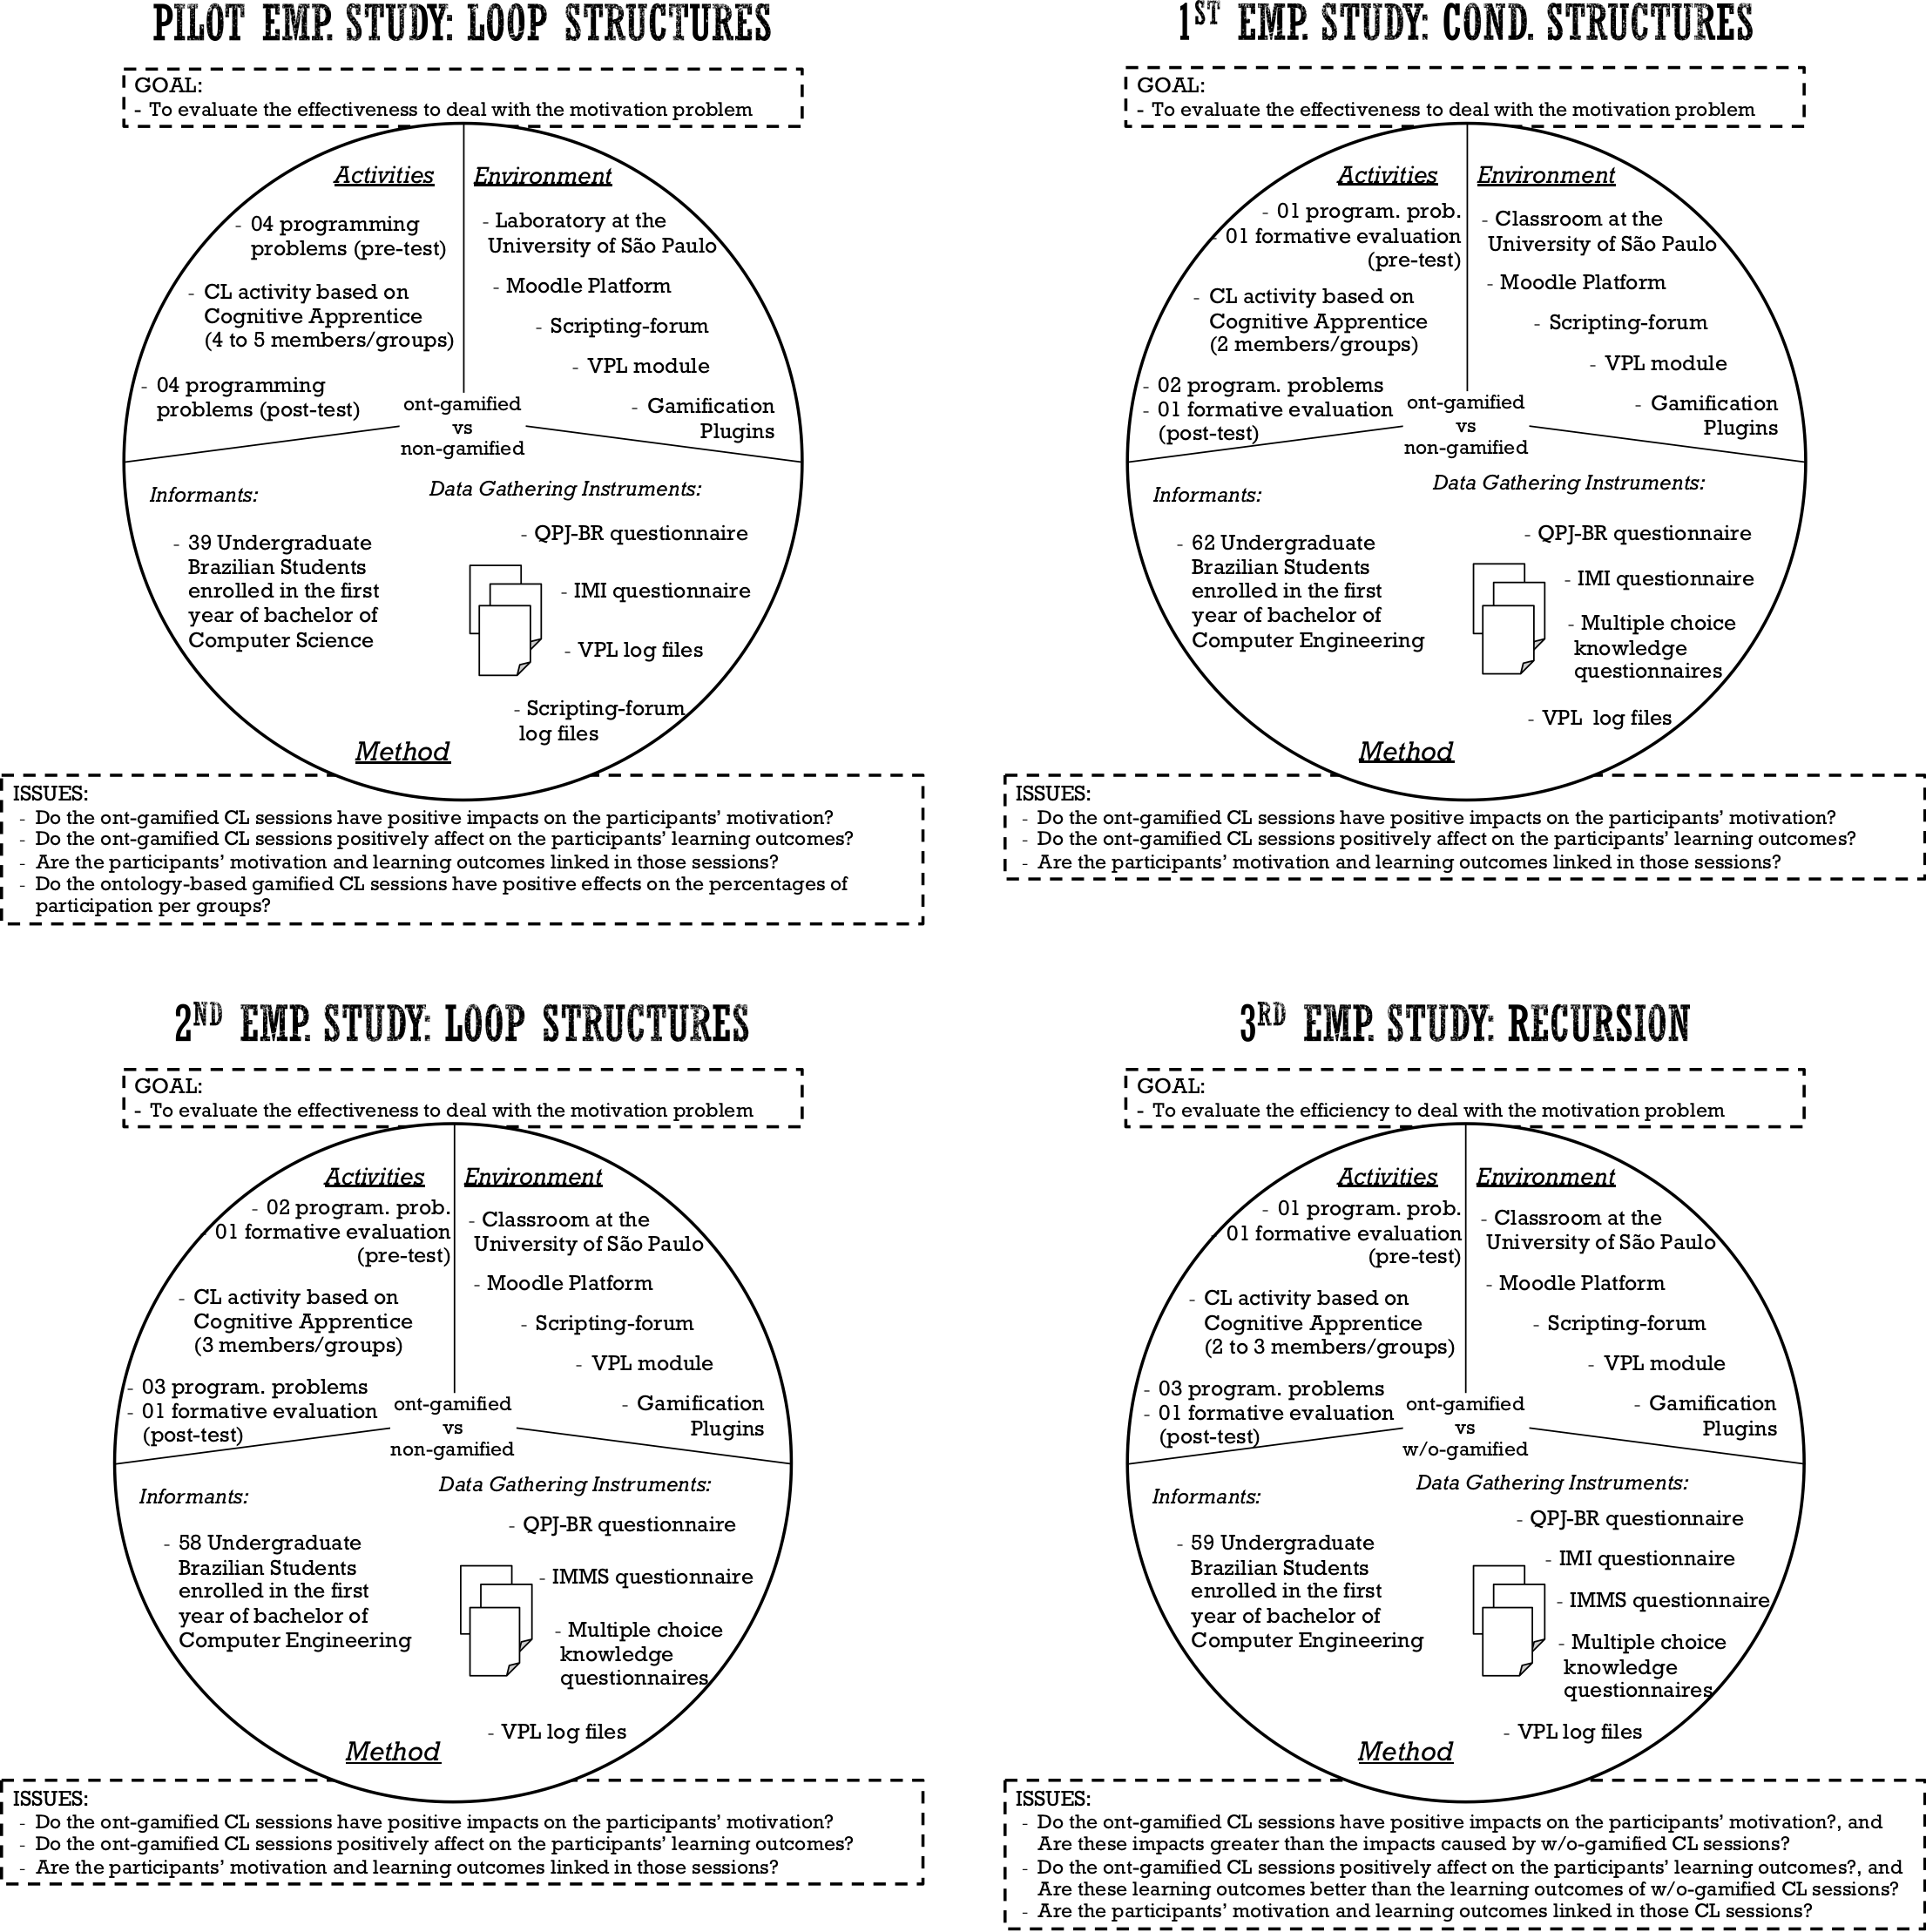
\includegraphics[width=1\textwidth]{images/chap-evaluation/graphical-empirical-studies.png}
 \fautor
\end{figure}


\chapter[Evaluation of the Ontological Engineering Approach to Gamify CL Scenarios]
{Evaluation of the Ontological Engineering Approach to Gamify Collaborative Learning Scenarios}
\label{chapter:evaluation}

This chapter undertakes the evaluation of the ontological engineering approach to gamify CL scenarios proposed in this dissertation.
To demonstrate the effectiveness and efficiency of my approach for dealing with motivational problems, four empirical studies, one pilot study and tree full-scale quasi-experimental studies were conducted at the University of São Paulo.
In these empirical studies, the participants were undergraduate Computer Science and Computer Engineering students who were enrolled in the course of Introduction to Computer Science.
They participated in CL sessions that were gamified using the knowledge in the ontology OntoGaCLeS.
Such CL sessions are known as ontology-based gamified CL sessions (\emph{ont-gamified} CL sessions), and the empirical studies, as reported in this chapter, investigated their effects on the participants' motivation and learning outcomes.
These effects were compared with the effects of the non-gamified CL sessions to evaluate their effectiveness, and to evaluate their efficiency, these effects were compared with the effects of CL sessions that were gamified using the conventional form - for these empirical studies, the conventional form to gamify CL sessions consisted in: the use of all the possible game elements provided by the gamification platform Moodle, gamification using one-size-fits-all approach without personalization of game elements, a gamification form where the instructional designer set up the game elements \emph{without} using any information given by the ontology OntoGaCLeS (\emph{w/o-gamified} CL sessions).

The chapter starts by presenting the formulation of the empirical studies in \autoref{sec:formulation-empirical-studies} in which the scoping, hypothesis, subjects, instruments and data collection procedure of the empirical studies are detailed.
Then, \autoref{sec:pilot-study} (Pilot Empirical Study: Data Analysis Results), \autoref{sec:first-study} (First Empirical Study: Data Analysis Results), \autoref{sec:second-study} (Second Empirical Study: Data Analysis Results), and \autoref{sec:third-study} (Third Empirical Study: Data Analysis Results) present the data analysis results of four empirical studies.
Finally, the interpretation and implication of obtained result in reference to the ontological engineering approach to gamify CL sessions are discussed in \autoref{sec:interpretation-implications}.

Part of the work described in this chapter will be published in the scientific article:

\begin{itemize}
\item
\aspas{\emph{Using Ontology and Gamification to Improve Students' Participation and Motivation in CSCL}} that will be published as chapter of book \aspas{\emph{First International Workshop on Social, Semantic, Adaptive and Gamification Techniques and Technologies for Distance Learning},} HEFA 2017 \cite{ChallcoMizoguchiIsotani2017}.
\end{itemize}

%%%%%%%%%%%%%%%%%%%%%%%%%%%%%%%%%%%%%%%%%%%%%%%%
\section{Formulation of the Empirical Studies}
\label{sec:formulation-empirical-studies}

For the instructional designers and practitioners, the ontological engineering approach to gamify CL scenarios aims to give structured guidance on how to gamify CL sessions for dealing with motivational problems in a scripted collaborative learning.
With this guidance given by intelligent tools that use the knowledge described in the ontology OntoGaCLeS - as was detailed in \autoref{chapter:computer-based-mechanisms-procedures}, the instructional designers and practitioners design, develop and execute CL sessions known as \aspas{\emph{ontology-based gamified CL sessions}} (\emph{ont-gamified}).
These CL sessions are considered the final product to be obtained by the ontological engineering approach to gamify CL scenarios, so that to demonstrate their effectiveness and efficacy to deal with motivational problems in a scripted collaborative learning, it is necessary to investigate the effects of the ont-gamified CL sessions on the participants' motivation and learning outcomes.
The correlation between these two variables has also been evaluated to verify if there is instructional benefits of gamification by motivating and engagement the participants in the scripted collaborative learning.

Improving the participation in CL sessions has also been hypothesized as one of the benefits from the ontological engineering approach to gamify CL scenarios.
Thereby, such benefit was evaluated in the pilot empirical study to demonstrate the effectiveness of this approach to deal with motivational problems in scripted collaborative learning.

\subsection{Scoping}
\label{subsec:scoping}

Following the template proposed by \citeonline{WohlinRunesonHstOhlssonRegnellWessln2012}, the scoping of empirical studies conducted as evaluation of the ontological engineering approach to gamify CL scenarios was:

Analyze \aspas{\emph{the effects of ont-gamified CL sessions on the participants' motivation and learning outcomes}} for the purpose of \aspas{\emph{validating the ontology engineering approach to gamify CL scenarios}} with respect to \aspas{\emph{the effectiveness and efficiency to deal with motivational problems in scripted collaborative learning}} from the point of view of the \aspas{\emph{instructional designers and practitioners who would like to know the benefits of these sessions}} in the context of \aspas{\emph{scripted collaborative learning.}}

Considering this scoping, the evaluation has been organized in four empirical studies shown in \autoref{fig:graphical-pilot-first-empirical-study} and \autoref{fig:graphical-second-third-empirical-study}.

\newpage
\begin{figure}[htb]
 \caption{Graphical representation of pilot and first empirical studies}
 \label{fig:graphical-pilot-first-empirical-study}
 \centering
 \begin{tabular}{c}
  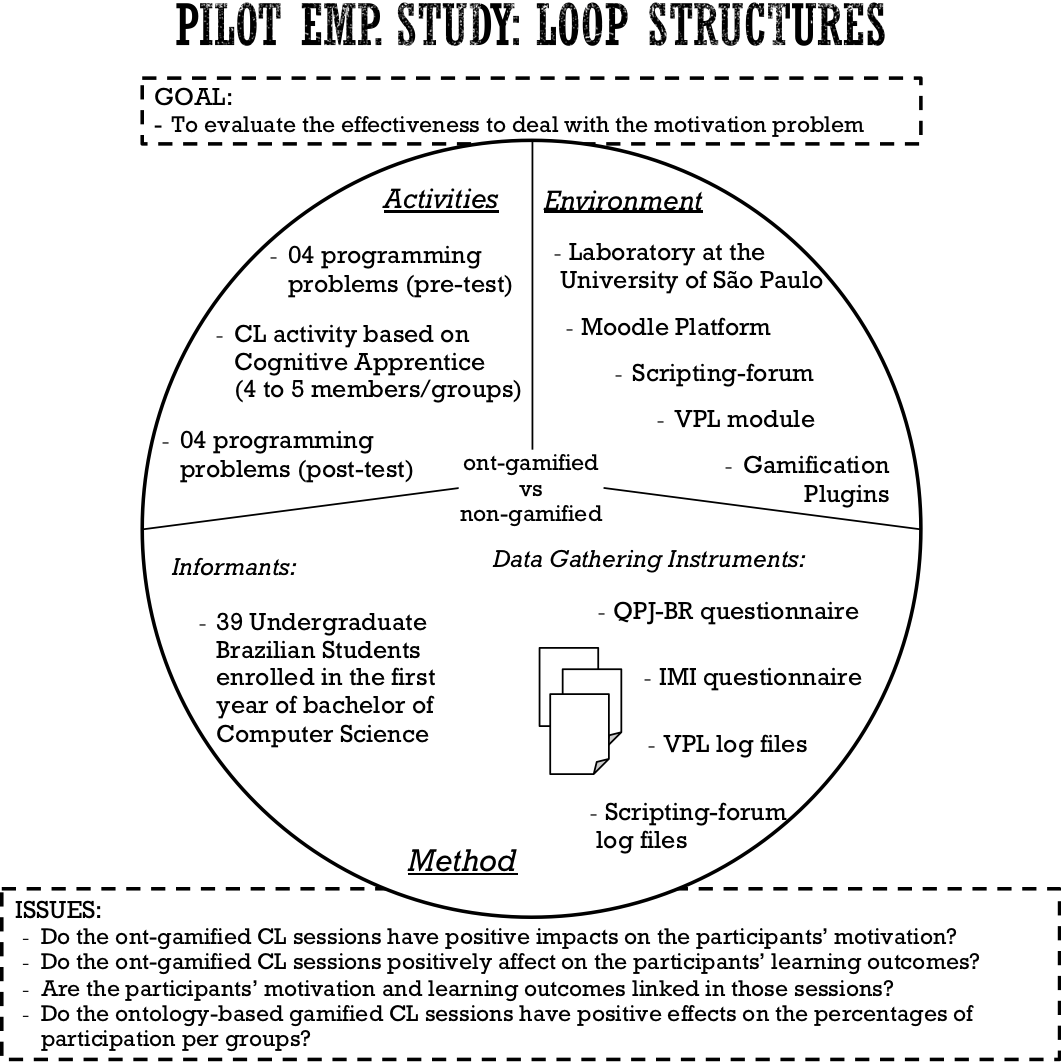
\includegraphics[width=0.63\textwidth]{images/chap-evaluation/graphical-pilot-empirical-study}\\
  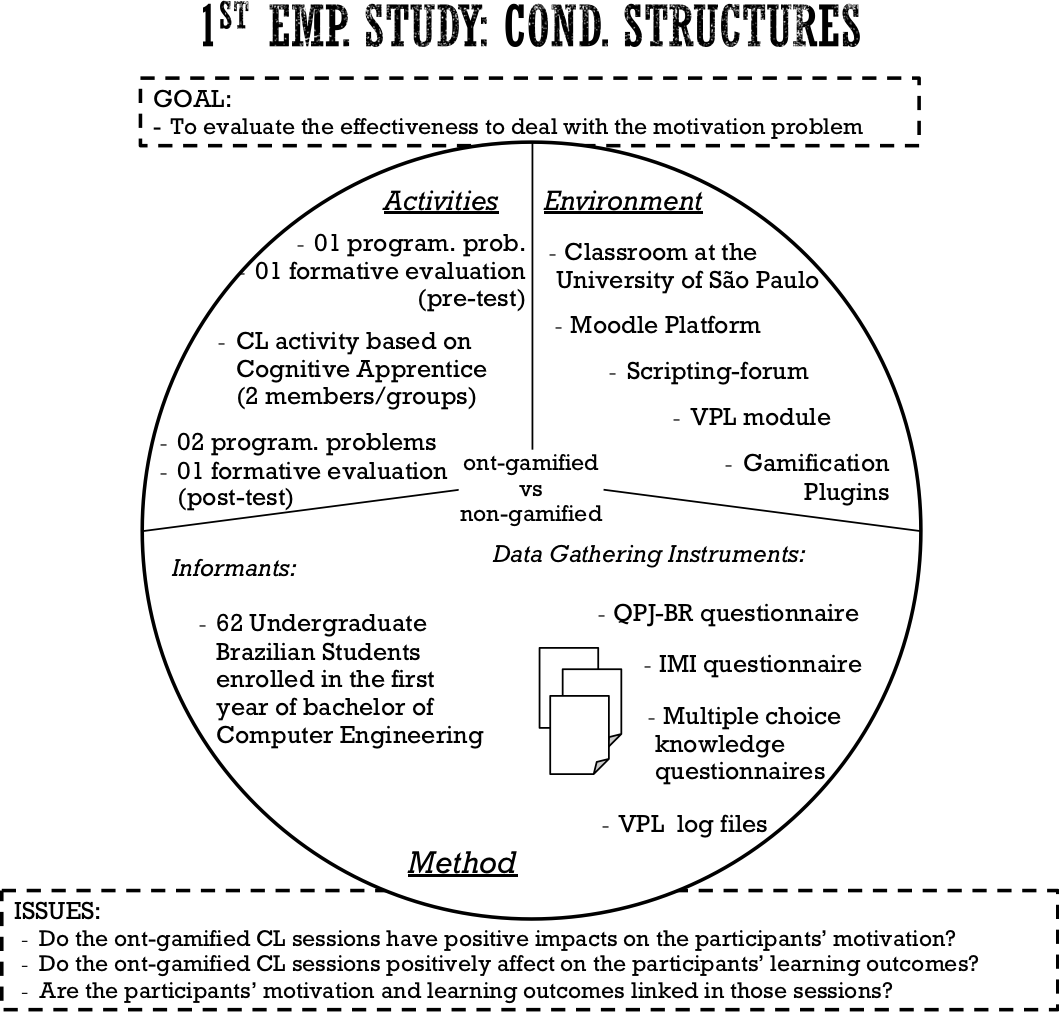
\includegraphics[width=0.63\textwidth]{images/chap-evaluation/graphical-first-empirical-study}
 \end{tabular}
 \fautor
\end{figure}

\newpage
\begin{figure}[htb]
 \caption{Graphical representation of second and third empirical studies}
 \label{fig:graphical-second-third-empirical-study}
 \centering
 \begin{tabular}{c}
  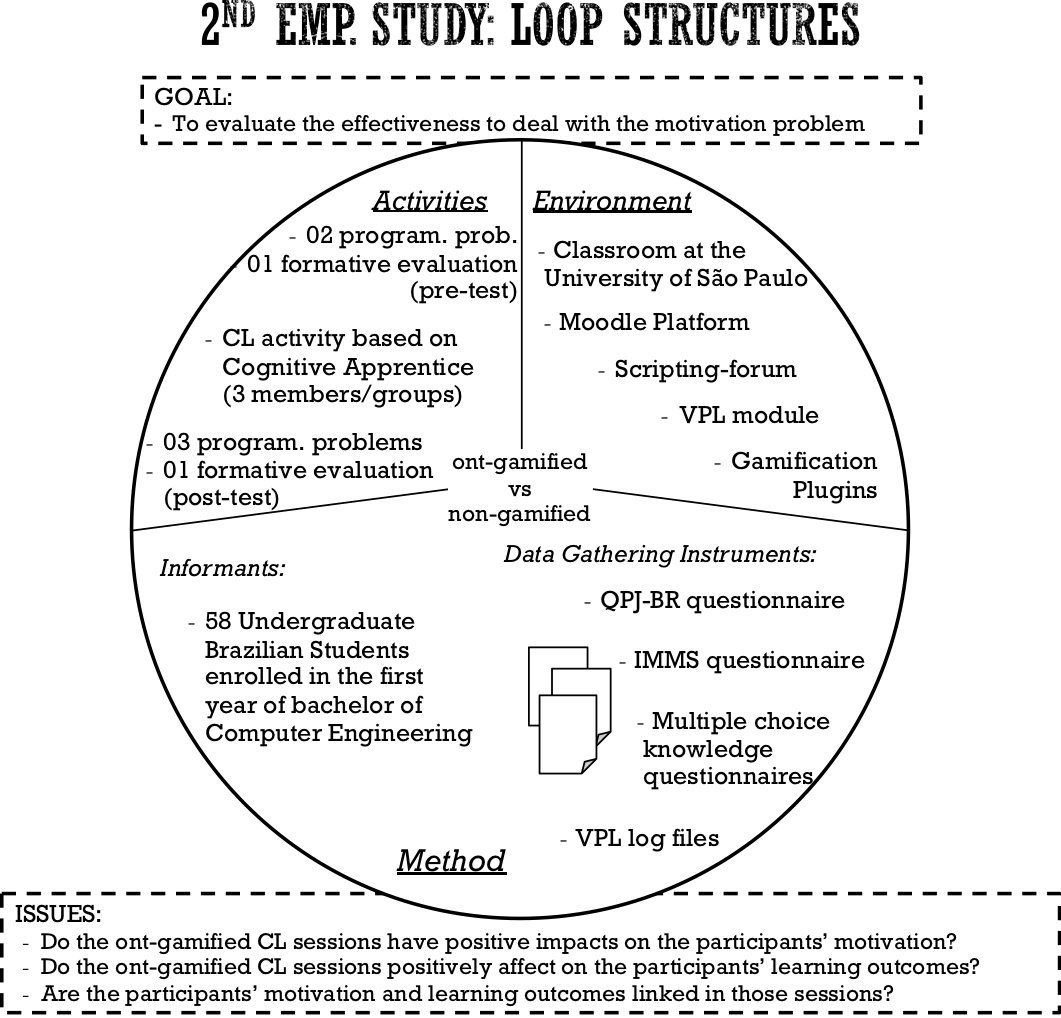
\includegraphics[width=0.63\textwidth]{images/chap-evaluation/graphical-second-empirical-study}\\
  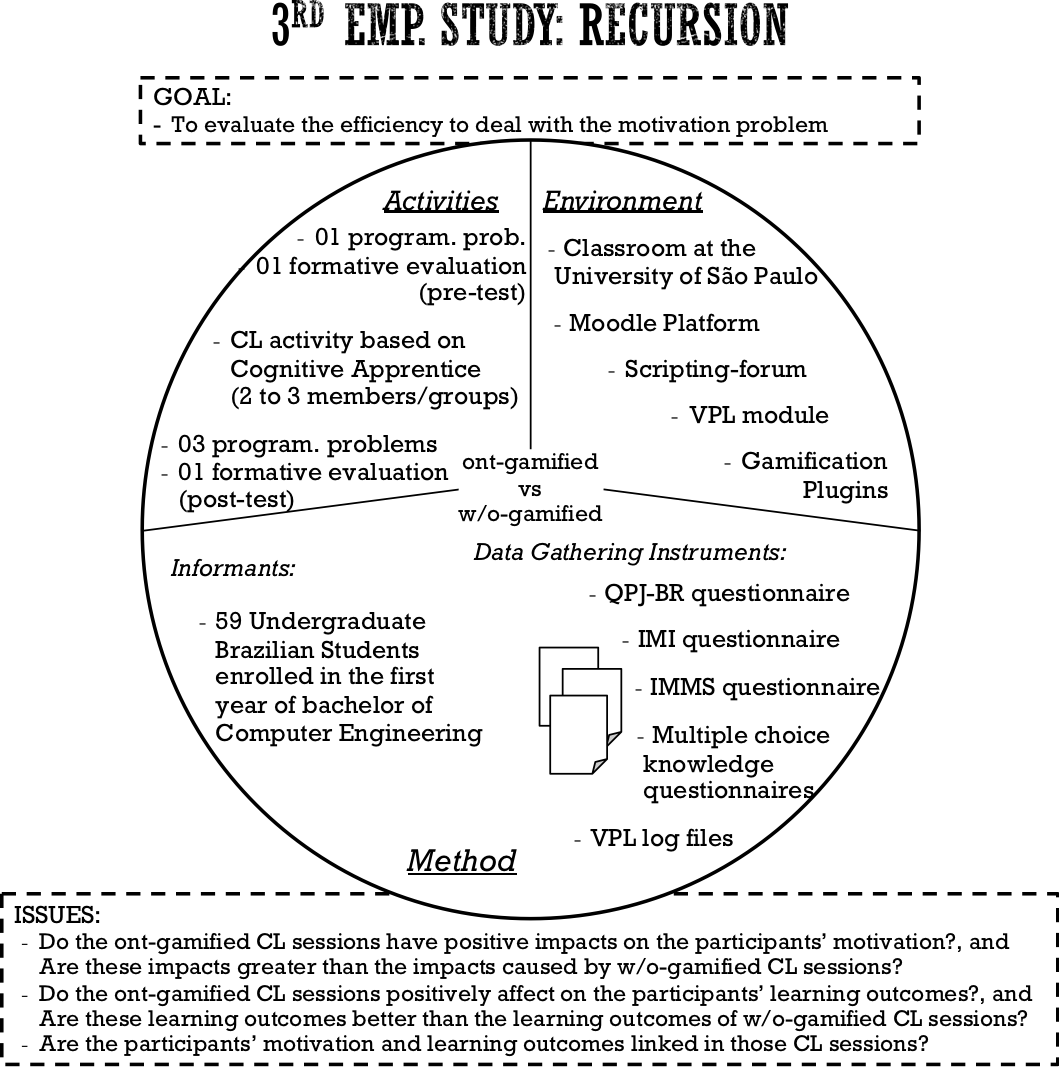
\includegraphics[width=0.63\textwidth]{images/chap-evaluation/graphical-third-empirical-study}
 \end{tabular}
 \fautor
\end{figure}

\newpage
The graphical representation for the empirical studies shown above (in \autoref{fig:graphical-pilot-first-empirical-study} and \autoref{fig:graphical-second-third-empirical-study}) is an adaptation of the Evaluand-oriented Responsive Evaluation Model (CSCL-EREM) diagram proposed by \citeonline{Jorrin-AbellanStakeMartinez-Mone2009}.
In the original version, the CSCL-EREM diagram is an artifact to summarize the characteristics that the researchers should be taken into account to conduct CSCL evaluations.
The diagram, employed here, is an adapted version of CSCL-EREM diagram in which only the relevant aspects of the \aspas{\emph{ontological engineering approach to gamify CL scenarios}} are summarized in the diagrams. These aspects are: the \emph{evaluand} indicated at the center of diagram;
the \emph{goal} and \emph{issues} shown in dashed frames at the top and bottom of circular diagram;
the educational setting features in respect to the learning \emph{environment} and \emph{activities} indicated on the left-upper and right-upper sides of the circular diagram; and
the \emph{informants} and \emph{data gathering instruments} employed during the evaluation \emph{method} shown at the bottom part of the circular diagram.

\textbf{Object of study}.
The object of study is the effects of ont-gamified CL sessions on the participants' motivation and learning outcomes.
The ont-gamified CL sessions have been gamified according to the suggestions given by intelligent tools, which in turn used the ontology OntoGaCLeS as information source to give these suggestions. 
Thus, the game elements were introduced intends to affect the participants' motivation, and in consequence, to produce better learning outcomes.
Thus, in the pilot, first and second empirical studies, the three issues addressed to evaluate the effectiveness of ont-gamified CL sessions for dealing with motivational problems were:

\begin{itemize}
\item Do the ont-gamified CL sessions have positive impacts on the participants' motivation?
\item Do the ont-gamified CL sessions affect on the participants' learning outcomes?
\item Are the participants' motivation and learning outcomes linked in those sessions?
\end{itemize}

The three issues addressed to evaluate the efficacy of ont-gamified CL sessions in the third empirical study were:

\begin{itemize}
\item Do the ont-gamified CL sessions have positive impacts on the participants' motivation?, and
Are the participants' motivation better in ont-gamified CL sessions than in w/o-gamified CL sessions?
\item Do the ont-gamified CL sessions affect on the participants' learning outcomes?, and
Are the participants' learning outcomes better in ont-gamified CL sessions than in w/o-gamified CL sessions?
\item Are the participants' motivation and learning outcomes linked in those sessions?
\end{itemize}

When the group members are adequately motivated to participate in a scripted collaborative learning, their engagement in the CL process will be increased, reducing the percentage of students who dropout the CL process.
These measurement of engagement was only evaluated in the pilot empirical study in which the CL activity assigned for the students was not mandatory. 
Thus, the issue addressed in the pilot empirical study is:

\begin{itemize}
\item Do the ont-gamified CL sessions have positive effects on the percentage of participation per groups?
\end{itemize}

These percentages of participation per group correspond to:
(1) the percentage of participants per groups \emph{having participation} that refers to a complete, semicomplete and incomplete participation level;
(2) the percentage of participants per groups having an \emph{adequate participation} that refers to a complete and semicomplete participation level;
(3) the percentage of participants per groups having \emph{incomplete participation} that refers to an incomplete and none participation level; and
(4) the percentage of participants per groups \emph{without participation} that refers to a none participation level.
Therefore, the participation levels are defined as:

\begin{itemize}
\item \emph{None participation level}: when the participant did not interact with other group members in CL sessions
\item \emph{Incomplete participation level}: when the participant interacted in CL sessions, but he/she did not complete all the necessary interactions
\item \emph{Semicomplete participation level}: when the student interacted in CL sessions performing all the necessary interactions, but he/she did not respond to all the requests made by other group members
\item \emph{Complete participation level}: when the participant interacted in CL sessions performing all the necessary interactions, and he/she responds to all the requests made by other group members
\end{itemize}
 
\textbf{Purpose}.
The empirical studies aim to validate the ontological engineering approach to gamify CL scenarios as a method to deal with motivational problems in scripted collaborative learning. 
Thus, the empirical studies were oriented to provide insights in what were the benefits of this approach in reference of the participants' motivation, and the consequence of these benefits in CL activities in which the CSCL scripts are used as a method to orchestrate and structure the collaboration among the participants in the CL.
Thus, in all the four empirical studies, this approach has been applied in CL activities with different levels of difficulty for their content-domains.
From the easiest to the hardest level of difficulty, the content-domains for the CL activities were: conditional structures, loop structures, and recursions (subjects of the course of Introduction to Computer Science).
The CSCL script used to structure and orchestrate the CL sessions was a CSCL script inspired by the Cognitive Apprentice theory.

\textbf{Quality focus}.
The \emph{effectiveness} was demonstrated by measuring the participants' motivation and learning outcomes in ont-gamified CL sessions, and then, by comparing these results against the results obtained in non-gamified CL sessions.
Therefore, the goal in the pilot, first and second empirical studies was to evaluate the effectiveness to deal with motivational problems, and the evaluand was: \emph{ont-gamified} vs \emph{non-gamified} CL sessions.

The \emph{efficiency} to deal with motivational problems was demonstrated by measuring the participants' motivation and learning outcomes in ont-gamified CL sessions, and then, by comparing these results against the results obtained in w/o-gamified CL sessions.
Therefore, the goal in the third empirical study was to evaluate the efficiency to deal with motivational problems, and the evaluand was: \emph{ont-gamified} vs \emph{w/o-gamified} CL sessions.

It is important to clarify here, that the motivation, as was explained in the \aspas{\emph{General Background}} (\autoref{chapter:general-background}), is a construct of different factors that explains the reason whereby a human behave or act.
It means that the factors to measure the participants' motivation vary according to the chosen theory to explain their behaviors and actions, vary in function of the context in which the theory is applied, and also, from the interest under study in each theory.
Thus, to validate the ontological engineering approach to gamify CL scenarios, two theories were used to measure the participants' motivation: the SDT theory, and the ARCS model of motivation.

\begin{itemize}
\item
In the SDT theory \cite{RyanDeci2000}, the construct of motivation is known as \emph{intrinsic motivation} that is defined as the degree of an individual owns to behave or act based on the self-determination and self-regulation.
Thus, the factors to measure the motivation are: the interest/enjoyment, perceived choice, felt of pressure/tension, effort/importance, perceived competence, value/usefulness and relatedness

\item
In the ARCS model \cite{Keller2009}, the construct of motivation is based on the expectancy-value theory in which is assumed that an individual is motivated if he/she sees value in his/her acts or behaviors and if there is an optimistic expectation for success in this acts or behaviors \cite{Wigfield1994}.
Hence, the factors for the construct of motivation in the ARCS model are: attention, relevance, confidence and satisfaction.
\end{itemize}

The data gathering instrument used to measure the intrinsic motivation was the adapter Portuguese version of Intrinsic Motivation Inventory (IMI) questionnaire.
It is important highlight here, that, to measure the intrinsic motivation using the IMI instrument, usually, not all factors are necessary.
The interest/enjoyment is only considered per se the self-report measure of intrinsic motivation.
The perceived choice and perceived competence are positive predictors, the pressure/tension is the negative predictor, the value/usefulness and effort/importance are factors to the internalization of motivation, and the relatedness factor is only applicable in context of interpersonal and friendship activities.
Therefore, in the pilot, first and third empirical studies the adapted Portuguese version of the IMI questionnaire has been used as data gathering instrument to measure:
the \emph{interest/enjoyment} as the factor directly related to measure the intrinsic motivation;
the \emph{perceived choice} as the only positive predictor;
the \emph{pressure/tension} as the negative predictor; and
the \emph{effort/importance} as the only factor related with the internalization of motivation.

In the second and third empirical studies, the data gathering instrument to measure the motivation as factors of the ARCS model was the adapter Portuguese version of Instructional Materials Motivation Survey (IMMS) questionnaire.
The measurement given by this instrument was the \aspas{\emph{level of motivation}} that consists in the factors: \emph{attention}, \emph{relevance} and \emph{satisfaction}.
The \aspas{\emph{confidence}} factor has been removed from the original ARCS model to avoid an overlapping with the factors of \aspas{\emph{perceived choiced}} measured by the IMI questionnaire because the confidence and perceived choice are both factors related to the self-regulation.
Thus, the \emph{level of motivation} is a constructor defined by the thesis author to refer the motivation that is completely separated from the intrinsic motivation.

\textbf{Perspective}.
The perspective for the empirical studies came from the viewpoint of the instructional designers and researchers.

\begin{itemize}
\item
Instructional designers would like to know the benefits of using ont-gamified CL sessions instead to use non-gamified CL sessions or w/o-gamified CL sessions.

\item
Researchers would like to know if the ontological engineering approach to gamify CL scenarios is an effective and efficient method to deal with motivational problems in the scripted collaborative learning.
\end{itemize}

\textbf{Context}.
The context in which the empirical studies has been conducted were the CL activities in which the CL sessions have been instantiated from a CSCL script inspired by an instructional/learning theory.
Particularly, in the empirical studies conducted to validate the ontological engineering approach to gamify the CL scenarios, the CSCL script used to design and to orchestrate the interaction of participants was a CSCL script inspired by the Cognitive Apprentice theory.
The domain-contents for which the scripts have been instantiated as CL sessions were three subjects for the course of \aspas{Introduction to Computer Science} with different difficulty levels.
From the easiest difficulty level to the most difficult level, these subjects were:
the \emph{conditional structures} for the first empirical study;
the \emph{loop structures} for the pilot and second empirical study; and
the \emph{recursion} for the third empirical study.

%% ========================== %%

\subsection{Hypothesis Formulation}

\emph{To evaluate the effectiveness for dealing with motivational problems} in scripted collaborative learning (First Goal, \emph{g1}), the first issue addressed in the pilot and first empirical studies was
\aspas{\emph{Do the ont-gamified CL sessions have positive impacts on the participants' motivation}?} by testing the:

\begin{description}
\item[Null hypothesis, $H_{null,IM,g1}$:]
\aspas{\emph{There was no significant difference between the intrinsic motivation of students who participated in ont-gamified CL sessions and the intrinsic motivation of students who participated in non-gamified CL sessions},} against the
\item[Alternative hypothesis, $H_{alt,IM,g1}$:]
\aspas{\emph{The intrinsic motivation of students who participated in ont-gamified CL sessions was greater than the intrinsic motivation of students who participated in non-gamified CL sessions}.}
\end{description}

In the second empirical study, this first issue was addressed by testing the:  

\begin{description}
\item[Null hypothesis, $H_{null,LoM,g1}$:]
\aspas{\emph{There was no significant difference between the level of motivation obtained by students who participated in ont-gamified CL sessions and the level of motivation obtained by students who participated in non-gamified CL sessions},} against the
\item[Alternative hypothesis, $H_{alt,LoM,g1}$:]
\aspas{\emph{The level of motivation obtained by students who participated in ont-gamified CL sessions was greater than the level of motivation obtained by students who participated in non-gamified CL sessions}.}
\end{description}

The second issue \aspas{\emph{Do the ont-gamified CL sessions affect on the participants' learning outcomes}?} has been addressed in the pilot, first and second empirical studies by testing the:

\begin{description}
\item[Null hypothesis, $H_{null,GSK,g1}$:]
\aspas{\emph{There was no significant difference between the gains in skill/knowledge obtained by students who participated in ont-gamified CL sessions and the gains in skill/knowledge obtained by students who participated in non-gamified CL sessions},} against the
\item[Alternative hypothesis, $H_{alt,GSK,g1}$:]
\aspas{\emph{The gains in skill/knowledge obtained by students who participated in ont-gamified CL sessions was different than the gains in skill/knowledge obtained by students who participated in non-gamified CL sessions}.}
\end{description}

In the pilot, first, and second empirical studies, the third issue \aspas{\emph{Are the participants' motivation and learning outcomes linked in either non-gamified or ont-gamified CL sessions}?} has been addressed by testing the:

\begin{description}
\item[Null hypothesis, $H_{null,\rho,g1}$:]
\aspas{\emph{There was no significant correlation between the participants' motivation and their gains of skill/knowledge in either the non-gamified CL sessions or the ont-gamified CL sessions},} against the
\item[Alternative hypothesis, $H_{alt,\rho,g1}$:]
\aspas{\emph{There was a significant correlation between the participants' motivation and their gains of skill/knowledge in either the non-gamified CL sessions or the ont-gamified CL sessions}.}
\end{description}

The four issue \aspas{\emph{Do the ont-gamified CL sessions have positive effects on the percentages of participation per groups}?} has been addressed in the pilot empirical study by testing the:

\begin{description}
\item[Null hypothesis, $H_{null,Pct,g1}$:]
\aspas{\emph{There was no significant difference in the percentages of participation per groups for ont-gamified and non-gamified CL sessions},} against the
\item[Alternative hypothesis, $H_{alt,Pct,g1}$:]
\aspas{\emph{The percentages of participation per groups in ont-gamified CL sessions are better than the percentage of participation per groups in non-gamified CL sessions}.}
\end{description}

\emph{To evaluate the efficiency for dealing with motivational problems} in scripted collaborative learning (Second Goal, \emph{g2}), the first issue  \aspas{\emph{Do the ont-gamified CL sessions have positive impacts on the participants' motivation?, and
Are the participants' motivation better in ont-gamified CL sessions than in w/o-gamified CL sessions}?} has been addressed in the third empirical study by testing the:

\begin{description}
\item[Null hypothesis, $H_{null,IM,g2}$:]
\aspas{\emph{There was no significant difference between the intrinsic motivation of students who participated in ont-gamified CL sessions and the intrinsic motivation of students who participated in w/o-gamified CL sessions},} against the
\item[Alternative hypothesis, $H_{alt,IM,g2}$:]
\aspas{\emph{The intrinsic motivation of students who participated in ont-gamified CL sessions was greater than the intrinsic motivation of students who participated in w/o-gamified CL sessions}.}
\end{description}

\begin{description}
\item[Null hypothesis, $H_{null,LoM,g2}$:]
\aspas{\emph{There was no significant difference between the level of motivation obtained by students who participated in ont-gamified CL sessions and the level of motivation obtained by students who participated w/o-gamified CL sessions},} against the
\item[Alternative hypothesis, $H_{alt,LoM,g2}$:]
\aspas{\emph{The level of motivation obtained by students who participated in ont-gamified CL sessions was greater than the level of motivation obtained by students who participated in w/o-gamified CL sessions}.}
\end{description}

In the third empirical study, the second issue \aspas{\emph{Do the ont-gamified CL sessions affect on the participants' learning outcomes?, and
Are the participants' learning outcomes better in ont-gamified CL sessions than in w/o-gamified CL sessions}?} has been addressed by testing the:

\begin{description}
\item[Null hypothesis, $H_{null,GSK,g2}$:]
\aspas{\emph{There was no significant difference between the gains in skill/knowledge obtained by students who participated in ont-gamified CL sessions and the gains in skill/knowledge obtained by students who participated in w/o-gamified CL sessions},} against the
\item[Alternative hypothesis, $H_{alt,GSK,g2}$:]
\aspas{\emph{The gains in skill/knowledge obtained by students who participated in ont-gamified CL sessions was greater than the gains in skill/knowledge obtained by students who participated in w/o-gamified CL sessions}.}
\end{description}

The third issue \aspas{\emph{Are the participants' motivation and learning outcomes linked in either ont-gamified or w/o-gamified CL sessions}?} has been addressed in the third empirical study by testing the:

\begin{description}
\item[Null hypothesis, $H_{null,\rho,g2}$:]
\aspas{\emph{There was no significant correlation between the participants' motivation and their gains of skill/knowledge in either the ont-gamified CL sessions or the w/o-gamified CL sessions},} against the
\item[Alternative hypothesis, $H_{alt,\rho,g2}$:]
\aspas{\emph{There was a significant correlation between the participants' motivation and their gains of skill/knowledge in either the ont-gamified CL sessions or the w/o-gamified CL sessions}.}
\end{description}

%% ========================== %%

\subsection{Variables Selection}

\autoref{tab:variables-empirical-studies} summarizes the variables involved in the empirical studies with the type of values for the variables and a brief explanation of them.
The independent variables \aspas{\emph{Type}} determined the type of CL sessions for which the evaluation of the ontological engineering approach to gamify CL scenario was carried out.
Thus, when the goal of the empirical study had been to evaluate the effectiveness of dealing with motivational problems ($g1$), the types of CL sessions were: 
ont-gamified CL sessions, and non-gamified CL sessions.
When the goal of the empirical study had been to evaluate the efficiency of dealing with the motivational problem ($g2$), the types of CL sessions were: ont-gamified CL sessions, and w/o-gamified CL sessions (CL sessions that were gamified using a conventional form to gamify).

\setlongtables{\small
\begin{longtable}{cllc}\caption{Independent and dependent variables for the empirical studies} \tabularnewline
\hline\hline
\multicolumn{1}{c}{Name}&\multicolumn{1}{c}{Values}&\multicolumn{1}{c}{Description}&\multicolumn{1}{c}{Studies}\tabularnewline
\hline
\endfirsthead\caption[]{\em (continued)} \tabularnewline
\hline
\multicolumn{1}{c}{Name}&\multicolumn{1}{c}{Values}&\multicolumn{1}{c}{Description}&\multicolumn{1}{c}{Studies}\tabularnewline
\hline
\endhead
\hline
\endfoot
\label{tab:variables-empirical-studies}
%\multicolumn{4}{l}{\emph{Dependent Variables}:}\tabularnewline \hline
Type &
\multicolumn{1}{p{2.5cm}}{\{\emph{ont-gamified}, \emph{non-gamified}\}} &
\multicolumn{1}{p{8.5cm}}{To evaluate the effectiveness, each student participated in one of these two types of CL scenarios during the empirical studies} &
\multicolumn{1}{p{1.5cm}}{\centering pilot, first, second}
\tabularnewline \hline

Type &
\multicolumn{1}{p{2.5cm}}{\{\emph{ont-gamified}, \emph{w/o-gamified}\}} &
\multicolumn{1}{p{8.5cm}}{To evaluate the efficiency, each student participated in one of these two types of CL scenarios during the empirical studies} &
\multicolumn{1}{p{1.5cm}}{\centering third}
\tabularnewline \hline

\multicolumn{4}{l}{\emph{Controller Variables}:}\tabularnewline \hline

CLRole &
\multicolumn{1}{p{2.5cm}}{\{\mbox{\emph{Master}}, \mbox{\emph{Apprentice}\}}} &
\multicolumn{1}{p{8.5cm}}{The CL role played by each participant in the CL sessions instantiated from a CSCL script inspired by the Cognitive Apprenticeship theory.
These roles are assigned for a participant according to his/her current knowledge/skill state} &
\multicolumn{1}{p{1.5cm}}{\centering pilot, first, second, third}
\tabularnewline \hline

\multicolumn{4}{l}{\emph{Dependent Variables}:}\tabularnewline \hline

\multicolumn{1}{p{2cm}}{\centering \mbox{Intrinsic} \mbox{Motivation}} &
\multicolumn{1}{p{2.5cm}}{\centering \emph{logits}} &
\multicolumn{1}{p{8.5cm}}{The intrinsic motivation estimates for the participants as the factors: interest/enjoyment, perceived choice, pressure/tension, and effort/importance. This dependent variable and its factors have been measured on a \emph{logit} scale} &
\multicolumn{1}{p{1.5cm}}{\centering pilot, first, third}
\tabularnewline \hline

\multicolumn{1}{p{2cm}}{\centering \mbox{Level} of \mbox{Motivation}} &
\multicolumn{1}{p{2.5cm}}{\centering \emph{logits}} &
\multicolumn{1}{p{8.5cm}}{The level of motivation estimates for the participants as the factors: attention, relevance, and satisfaction. This dependent variable and its factors have been measured on a \emph{logit} scale} &
\multicolumn{1}{p{1.5cm}}{\centering second, third}
\tabularnewline \hline

\multicolumn{1}{p{2cm}}{\centering \mbox{Gains} in \mbox{Skill}/\mbox{Knowledge}} &
\multicolumn{1}{p{2.5cm}}{\centering \emph{logits}} &
\multicolumn{1}{p{8.5cm}}{The gains in skill/knowledge for the participants were measured as learning outcomes employing irt-models for programming problems and multiple choice knowledge questionnaires on a \emph{logit} scale} &
\multicolumn{1}{p{1.5cm}}{\centering pilot, first, second, third}
\tabularnewline \hline


\multicolumn{1}{p{2cm}}{\centering Pct. of \mbox{Participation} per \mbox{Groups}} &
\multicolumn{1}{p{2.5cm}}{\centering \mbox{\emph{Pct.}}} &
\multicolumn{1}{p{8.5cm}}{The percentages of participation per group. These percentages correspond to the 
pct. of students without participation, pct. of students having participation, pct. of students having incomplete participation, and pct. of students having adequate participation.} &
\multicolumn{1}{p{1.5cm}}{\centering pilot}
\tabularnewline \hline

\end{longtable}}

%% ========================== %%

\subsection{Selection of Subjects}

According to the real situation in which the empirical studies were carried out, the subjects for the empirical studies were chosen based on convenience. 
The subjects were students signed-up in the course of Introduction to Computer Science taught by the Prof. Seiji Isotani to the graduate programs in Computer Science and Computer Engineering at the University of São Paulo during the second semester of 2016 (August -  December) and the first semester of 2017 (March - July).
Thus, the selection of subjects, described as informants in the CSCL-EREM diagrams of \autoref{fig:graphical-pilot-first-empirical-study} and \autoref{fig:graphical-second-third-empirical-study} for each empirical study, were: 

\begin{description}
\item[For the pilot empirical study,]
39 undergraduate Brazilian students enrolled in the first year of bachelor of Computer Science at the University of São Paulo.
\item[For the first empirical study,]
62 undergraduate Brazilian students enrolled in the first year of bachelor of Computer Engineering at the University of São Paulo.
\item[For the second empirical study,]
58 undergraduate Brazilian students enrolled in the first year of bachelor of Computer Engineering at the University of São Paulo.
\item[For the third empirical study,]
59 undergraduate Brazilian students enrolled in the first year of bachelor of Computer Engineering at the University of São Paulo.
\end{description}

The participants in the empirical studies were chosen from a homogeneous population in the age range from 17 to 25 years old, sharing the same social-economy status and culture.

%% ========================== %%
\subsection{Design}

Employing the scoping, hypothesis formulation, variables selection, and selection of subjects detailed in the previous subsections, the principles to design the four empirical studies were:

\begin{description}
\item[Randomization.] The CL role was not randomly assigned to the students in the empirical studies.
If the student has known how to use the cognitive or meta-cognitive skill and had experience in how to use this skill, he/she played the master role, otherwise the student played the apprentice role.
The students as subjects of empirical studies were not selected randomly, they were the students signed-up to the course of Introduction to Computer Science at the University of São Paulo during the second semester of 2016 and the first semester of 2017.
With these students as subjects of empirical studies, a theory-driven group formation was carried out according to the pseudo-algorithm proposed by \citeonline{IsotaniMizoguchi2008a}; and then, randomly, one half of the groups were assigned to participate in one of two types of CL sessions that are defined as \emph{evaluand} in each empirical study, whereas the other half of groups were assigned to participate in the other type of CL sessions.
Thus, for the pilot, first and second empirical studies, one half of groups defined by the theory-driven group formation was randomly chosen to participate in non-gamified CL sessions, and the other half of groups were chosen to participate in ont-gamified CL sessions.
For the third empirical study, one half of groups were randomly participated in ont-gamified CL sessions, and the other half of groups participated in w/o-gamified CL sessions.

\item[Blocking.]
No systematic approach to block the independent and control variables applied in the empirical studies.
The decision to assign CL roles for the students as subject of empirical studies was based on their current skill/knowledge states, so that this determination could be contemplated a way to block the effect of students having different levels of knowledge and having different levels of cognitive or meta-cognitive skills. 

\item[Balancing.] The empirical studies did not have a balanced design because they were conducted in real situations given by the course of Introduction to Computer Science at the University of São Paulo during the 2nd semester of 2016 and the 1st semester of 2017.
\end{description}

According to the principles mentioned above, the four empirical studies have been defined as quasi-experiments with a $2\times2$ factorial design, and with a randomized assignment of the type of CL session for the groups defined by the theory-driven group formation proposed by \citeonline{IsotaniMizoguchi2008a}. 
Furthermore, each empirical study has been conducted in three phases: pre-test phase, intervention phase, and post-test phase.
During the pre-test phase, the skill and knowledge levels of students were estimated to assign the CL roles.
The necessary and desired conditions to assign Player roles for the participants have also been obtained in the pre-test phase through a questionnaire of player types.
The gains in skill/knowledge for the participants were estimated as the difference of their skill and knowledge obtained in the post-test phase and their skill and knowledge obtained in the pre-test phase.
In the post-test phase, motivation surveys were applied to the participants for measuring the participants' motivation as measurement of the intrinsic motivation and the level of motivation.

%% ========================== %%
\subsection{Instrumentation}
\label{subsec:instrumentation}

As was shown in the conceptual flow to gamify CL sessions using the knowledge described in the ontology OntoGaCLeS (\autoref{fig:conceptual-flow-gamify-cl-sessions}), to obtain the ont-gamified CL sessions, it is necessary to have information about the necessary and desired conditions to assign player roles for the students in each empirical study.
This information has been collected in the Moodle platform through a Web-based version of QPJ-BR questionnaire \cite{AndradeMarquesBittencourtIsotani2016} - that is detailed in \autoref{annex:QPJ-BR-questionnaire}.

Programming problem tasks and multiple-choice knowledge questionnaires were used as information sources to estimate the skill and knowledge of participants in the pre-test and post-test phases.
The skill and knowledge estimates from pre-test were also been used to assign the CL roles for the participants of empirical studies.
\autoref{tab:programming-problem-multiple-choice-questionnaires} shows the programming problem tasks and multiple-choice knowledge questionnaires employed in the empirical studies.
All the programming problem tasks were implemented in an adapted version of \emph{VPL module}\footnote{Virtual Programming Lab for Moodle 2 with screen and code recordings - \url{https://github.com/geiser/moodle-mod_vpl}}, and the multiple-choice knowledge questionnaires were developed using the \emph{AMC software}\footnote{Software to create multiple-choice questionnaires - \url{https://www.auto-multiple-choice.net/}}

\setlongtables{\small
\begin{longtable}{cccp{9cm}c}\caption{Programming problem tasks and multiple choice knowledge questionnaires} \tabularnewline
\hline\hline
\multicolumn{1}{c}{Code}&\multicolumn{1}{c}{Study}&\multicolumn{1}{c}{Phase}&\multicolumn{1}{c}{Title}&\multicolumn{1}{c}{\autoref{annex:data-gathering-instruments-skill-knowledge}}\tabularnewline
\hline
\endfirsthead\caption[]{\em (continued)} \tabularnewline
\hline
\multicolumn{1}{c}{Code}&\multicolumn{1}{c}{Study}&\multicolumn{1}{c}{Phase}&\multicolumn{1}{c}{Title}&\multicolumn{1}{c}{\autoref{annex:data-gathering-instruments-skill-knowledge}}\tabularnewline
\hline
\endhead
\hline
%\multicolumn{6}{r}{\tiny Signif. codes:  0 \aspas{**} 0.01 \aspas{*} 0.05}
\endfoot
\label{tab:programming-problem-multiple-choice-questionnaires}

P1'&pilot&pre-test&
Programming Problem: Calculate the proper divisors of a number (\emph{Divisores próprios})
&\autoref{annex:pilot-study-p1} \tabularnewline

P2'&pilot&pre-test&
Programming Problem: Calculate the sum of prime divisors of number (\emph{Soma dos divisores próprios})
&\autoref{annex:pilot-study-p2} \tabularnewline

P3'&pilot&pre-test&
Programming Problem: Calculate distance of rebounds for an elastic ball (\emph{Distância dos rebates da bola de elástico})
&\autoref{annex:pilot-study-p3} \tabularnewline

P4'&pilot&pre-test&
Programming Problem: Calculate the maximum length of a hailstone sequence (\emph{Máximo comprimento das sequências de números granizo})&
\autoref{annex:pilot-study-p4} \tabularnewline

PA'&pilot&post-test&
Programming Problem: Calculate the Inverse Fibonacci sequence on base $n$ and $m$ (\emph{Sequência inversa Fibonacci de base $n$ e $m$})&
\autoref{annex:pilot-study-pA} \tabularnewline

PB'&pilot&post-test&
Programming Problem: Calculate the absolute difference between odd and even numbers in an inverse Fibonacci sequence (\emph{Diferença absoluta entre os números pares e ímpares na sequência inversa Fibonacci})&
\autoref{annex:pilot-study-pB} \tabularnewline

PC'&pilot&post-test&
Programming Problem: Calculate the i-th prize of a machine slot (\emph{O i-ésimo prêmio da caça-níquel)})&
\autoref{annex:pilot-study-pC} \tabularnewline

PD'&pilot&post-test&
Programming Problem: Calculate the highest prize of a machine slot (\emph{Ganhando o prêmio maior da caça-níquel})&
\autoref{annex:pilot-study-pD} \tabularnewline

P1&first&pre-test&
Programming Problem: Develop a simple virtual temperature monitor(\emph{Monitor de Temperatura Virtual})&
\autoref{annex:first-study-p1}\tabularnewline

p1a&first&pre-test&
Formative Evaluation: Multiple choice knowledge questionnaires of cond. structures (\emph{provinha1a})&
\autoref{annex:first-study-pre}\tabularnewline


PA&first&post-test&
Programming Problem: Develop a Basal Metabolic Rate (\emph{TMB - Taxa Metabólica Basal})&
\autoref{annex:first-study-pA}\tabularnewline

PB&first&post-test&
Programming Problem: Develop a diet calculator (\emph{Calculadora de dieta})&
\autoref{annex:first-study-pB}\tabularnewline

p1b&first&pre-test&
Formative Evaluation: Multiple choice knowledge questionnaires of cond. structures (\emph{provinha1b})&
\autoref{annex:first-study-pos}\tabularnewline

P2&second&pre-test&
Programming Problem: Calculate the proper divisors of a number (\emph{Divisores próprios})&
\autoref{annex:second-study-p2}\tabularnewline

P3&second&pre-test&
Programming Problem: Calculate the maximum length of a hailstone sequence (\emph{Máximo comprimento das sequências de números granizo})&
\autoref{annex:second-study-p3}\tabularnewline

p2a&second&pre-test&
Formative Evaluation: Multiple choice knowledge questionnaires of loop structures (\emph{provinha2a})&
\autoref{annex:second-study-pre}\tabularnewline

PC&second&post-test&
Programming Problem: Calculate a geometric sequence (\emph{Sequências de potências})&
\autoref{annex:second-study-pC}\tabularnewline

PD&second&post-test&
Programming Problem: Calculate global minimum coin changes (\emph{Caixa eletrônico})&
\autoref{annex:second-study-pD}\tabularnewline

PE&second&post-test&
Programming Problem: Count number of semi-primes for RSA (\emph{Contagem de semi-primos para o algoritmo RSA})&
\autoref{annex:second-study-pE}\tabularnewline

p2b&second&post-test&
Formative Evaluation: Multiple choice knowledge questionnaires of loop structures (\emph{provinha2b})&
\autoref{annex:second-study-pos}\tabularnewline

P4&third&pre-test&
Programming Problem: Calculate fibonacci polynomials (\emph{Polinômios de Fibonacci})&
\autoref{annex:third-study-p4}\tabularnewline

p3a&third&pre-test&
Formative Evaluation: Multiple choice knowledge questionnaires of recursion (\emph{provinha3a})&
\autoref{annex:third-study-pre}\tabularnewline

PF&third&post-test&
Programming Problem: Generation of planning poker sequence (\emph{Planning Poker})&
\autoref{annex:third-study-pF}\tabularnewline

PG&third&post-test&
Programming Problem: Counting palindromes (\emph{Contagem de palindromos})&
\autoref{annex:third-study-pG}\tabularnewline

PH&third&post-test&
Programming Problem: Maze solving algorithm (\emph{A saída do labirinto})&
\autoref{annex:third-study-pH}\tabularnewline

p3c&third&post-test&
Formative Evaluation: Multiple choice knowledge questionnaires of recursion (\emph{provinha3c})&
\autoref{annex:third-study-pos}\tabularnewline

\hline
\end{longtable}}


In the empirical studies, the data gathering instruments used to measure the participants' motivation were:

\begin{itemize}
\item
a Web-based questionnaire for the adapted Portuguese version of the Intrinsic Motivation Inventory (\autoref{annex:data-gathering-instruments-motivation}:
\autoref{annex:IMI-pilot-study}) employed in the pilot empirical study to gather information related to the participants' intrinsic motivation

\item
a Paper-based questionnaire for the adapted Portuguese version of the Intrinsic Motivation Inventory (\autoref{annex:data-gathering-instruments-motivation}:
\autoref{annex:IMI-first-study}) employed in the first empirical study to gather information related to the participants' intrinsic motivation

\item
a Paper-based questionnaire for the adapted Portuguese version of the Instructional Materials Motivation Survey (\autoref{annex:data-gathering-instruments-motivation}:
\autoref{annex:IMMS-second-study}) employed in the second empirical study to gather information related to the participants' level of motivation

\item
a Web-based questionnaire for the adapted Portuguese version of the Intrinsic Motivation Inventory and the adapted Portuguese Instructional Materials Motivation Survey (\autoref{annex:data-gathering-instruments-motivation}:
\autoref{annex:IMI-IMMS-third-study}) employed in the third empirical study to gather information related to the participants' intrinsic motivation and level of motivation
\end{itemize}

The ont-gamified CL sessions in the empirical studies were obtained through the conceptual flow to gamify CL sessions shown in \autoref{fig:conceptual-flow-gamify-cl-sessions}, so that the information encoded in the \aspas{\emph{ontological model to apply gamification as persuasive technology in CL scenarios based on the Cognitive Apprenticeship theory and with the player roles based on the Yee's model to personalize the gamification}} has been used with the \emph{Gamification plug-in}s in the Moodle platform to define the ont-gamified CL sessions.
However, due to the lack of automatic support given by the Gamification plug-ins to set and to configure the game elements in the Moodle learning environment, the gamification of CL sessions was not carried out using all the three ontological structures to represent gamified CL scenarios described in this ontology-based model.
Thus, only two of three ontological structures were employed simultaneously in each empirical study to set and configure the Gamification plug-ins:

\begin{itemize}
\item For the pilot, first and second empirical studies, the ontological structures to represent \aspas{\emph{Gamified Cognitive Apprenticeship Scenario for Master/Yee Achiever and Apprentice/Yee Achiever}} and \aspas{\emph{Gamified Cognitive Apprenticeship Scenario for Master/Yee Socializer and Apprentice/Yee Socializer}} were used to obtain the ont-gamified CL sessions.

\item For the third empirical study, the ontological structures to represent \aspas{\emph{Gamified Cognitive Apprenticeship Scenario for Master/Yee Achiever and Apprentice/Yee Achiever}} and \aspas{\emph{Gamified Cognitive Apprenticeship Scenario for Master/Social Achiever and Apprentice/Social Achiever}} were used to obtain the ont-gamified CL sessions.
%detail in appendix the screens and CSCL script-
\end{itemize}

Finally, in all the types of CL sessions (ont-gamified CL sessions, non-gamified CL sessions, and w/o-gamified CL sessions), a CSCL script inspired by the Cognitive Apprenticeship theory and illustrated in \autoref{fig:cognitive-apprenticeship-cscl-script} was used as a method to orchestrate and structure the collaboration among the participants.
This script was implemented as CL activities in the Moodle platform employing the \emph{Scripting-forum module}\footnote{Available at the URL: \url{https://github.com/geiser/moodle\_scripting\_forum}}.


%% ========================== %%
\subsection{Schedule, Timing, and Data Collection Procedure}
\label{subsec:data-collection-procedure}

\textbf{Preparation:} The aspects under study in the empirical studies and the hypotheses stated in this dissertation were not informed to the participants (students) of the empirical studies, but they were aware that the researcher wanted to use the data gathered by their participation in the course.
All participants (students) were guaranteed anonymity, and all materials that were used in the data collection procedure were prepared in advance.
Before the intervention phase, as part of the preparation phase, the students were instructed in how to participate in CL activities using the \emph{Scripting-forum module} in the Moodle platform.

\subsubsection{Execution: Pilot Empirical Study}

The pilot empirical study was executed over three weeks with the schedule, timing, and data collection procedure showed in \autoref{fig:data-collection-procedure-pilot-study}.~

\begin{figure}[htb]
 \caption{Diagram of the schedule, timing and data collection procedure in the pilot empirical study}
 \label{fig:data-collection-procedure-pilot-study}
 \centering
 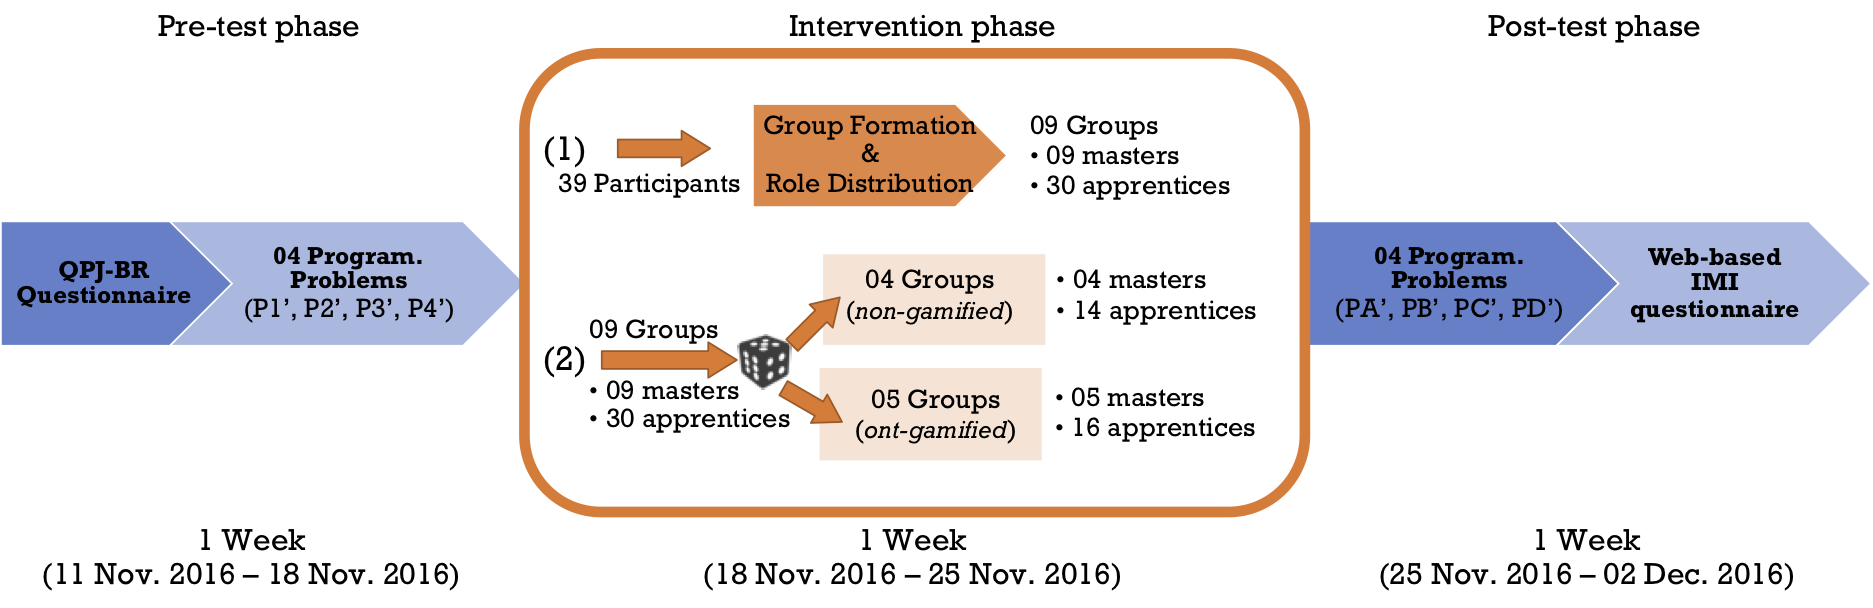
\includegraphics[width=1\textwidth]{images/chap-evaluation/data-collection-procedure-pilot-study.png}
 \fautor
\end{figure}

\textbf{During the pre-test phase (1 week)}, from 11 November 2016 to 18 November 2016, the Web-based QPJ-BR questionnaire has been answered by all the participants through the Moodle platform using the \emph{Questionnaire module}\footnote{Available at the URL: \url{https://github.com/geiser/moodle-mod\_questionnaire}}.
During this phase, to gather data related to the skill/knowledge, four programming problem tasks (P1', P2', P3', and P4' - detailed in \autoref{tab:programming-problem-multiple-choice-questionnaires}) have also been solved by the students in the Moodle platform using the VPL module.

\textbf{During the intervention phase (1 week)}, from 18 November 2016 to 25 November 2016, the thirty-nine students participated in either non-gamified CL sessions or ont-gamified CL sessions.
These students were formed into nine groups of four or five members with nine masters and thirty apprentices assigned according to the theory-driven group formation \cite{IsotaniMizoguchi2008a}.
Four of these nine groups participated in non-gamified CL sessions, and five groups participated in ont-gamified CL sessions.

The ontological structures to represent \aspas{\emph{Gamified Cognitive Apprenticeship Scenario for Master/Yee Achiever and Apprentice/Yee Achiever}} and \aspas{\emph{Gamified Cognitive Apprenticeship Scenario for Master/Yee Socializer and Apprentice/Yee Socializer}} were used to obtain the ont-gamified CL sessions in which:

\begin{itemize}
\item The students who had more liking for achievement-components than positive liking for social-components were assigned to play the \emph{Yee Achiever role} in gamified CL sessions instantiated from the ontological structure \aspas{\emph{Gamified Cognitive Apprenticeship Scenario for Master/Yee Achiever and Apprentice/Yee Achiever}} to support a CL Gameplay experience of \emph{individual competition}.

\item The students who had more positive liking for social-components than positive liking for achievement-components were assigned to play the \emph{Yee Socializer role} in gamified CL sessions instantiated from the ontological structure \aspas{\emph{Gamified Cognitive Apprenticeship Scenario for Master/Yee Socializer and Apprentice/Yee Socializer}} to support a CL Gameplay experience of \emph{cooperative competition}.
\end{itemize}

\textbf{During the post-test phase (1 week)}, from 25 November 2016 to 02 December 2016, to gather data related to the skill/knowledge, four programming problem tasks (PA', PB', PC', and PD' - detailed in \autoref{tab:programming-problem-multiple-choice-questionnaires}) have been solved by the students in the Moodle platform using the VPL module.
The students also answered the IMI questionnaire through the Moodle platform using the \emph{Questionnaire module} to gather data related to the participants' intrinsic motivation.

\subsubsection{Execution: First Empirical Study}

The first empirical study was executed over four weeks and four days with the schedule, timing, and data collection procedure showed in \autoref{fig:data-collection-procedure-first-study}.

\begin{figure}[htb]
 \caption{Diagram of the schedule, timing and data collection procedure in the first empirical study}
 \label{fig:data-collection-procedure-first-study}
 \centering
 \includegraphics[width=1\textwidth]{images/chap-evaluation/data-collection-procedure-first-study.png}
 \fautor
\end{figure}

\textbf{During the pre-test phase (1 week)}, from 23 March 2017 to 30 March 2017, to gather information of students' preference related to their liking for game-components, the Web-based QPJ-BR questionnaire has been answered by all the participants through the Moodle platform using the \emph{Questionnaire module}.
Data related to the participants' initial skill/knowledge were gathered from one programming problem task (P1) and one multiple-choice knowledge questionnaire of conditional structures (p1a), both instruments are detailed in \autoref{tab:programming-problem-multiple-choice-questionnaires}. 
The programming problem task (P1) was solved by the students in the Moodle platform using the \emph{VPL module}, and the students answered the multiple-choice knowledge questionnaire (p1a) - during 2 hours on March, 30th - at the classroom in the University of São Paulo as a formative evaluation during the course of Introduction to Computer Science. 

\textbf{During the intervention phase (2 weeks \& 4 days)}, from 31 March 2017 to 18 April 2017, the sixty-two students participated in either non-gamified CL sessions or ont-gamified CL sessions.
These students were formed into thirty-one groups of two members with thirty-one masters and thirty-one apprentices assigned according to the theory-driven group formation \cite{IsotaniMizoguchi2008a}. 
Sixteen of thirty one groups participated in non-gamified CL sessions, and fifteen groups participated in ont-gamified CL sessions.

The ontological structures to represent \aspas{\emph{Gamified Cognitive Apprenticeship Scenario for Master/Yee Achiever and Apprentice/Yee Achiever}} and \aspas{\emph{Gamified Cognitive Apprenticeship Scenario for Master/Yee Socializer and Apprentice/Yee Socializer}} were used to obtain the ont-gamified CL sessions in which:

\begin{itemize}
\item The students who had more liking for achievement-components than positive liking for social-components were assigned to play the \emph{Yee Achiever role} in gamified CL sessions instantiated from the ontological structure \aspas{\emph{Gamified Cognitive Apprenticeship Scenario for Master/Yee Achiever and Apprentice/Yee Achiever}} to support a CL Gameplay experience of \emph{individual competition}.
\item The students who had more positive liking for social-components than positive liking for achievement-components were assigned to play the \emph{Yee Socializer role} in gamified CL sessions instantiated from the ontological structure \aspas{\emph{Gamified Cognitive Apprenticeship Scenario for Master/Yee Socializer and Apprentice/Yee Socializer}} to support a CL Gameplay experience of \emph{cooperative competition}.
\end{itemize}

\textbf{During the post-test phase (1 week)}, from 18 April 2017 to 25 April 2017, to gather data related to the skill/knowledge, the multiple-choice knowledge questionnaire of conditional structures (p1b) was answered by the participant’s - during 2 hours on April, 18th - at the classroom in the University of São Paulo as a formative evaluation in the course of Introduction to Computer Science.
Two programming problem tasks (PA, PB - detailed in \autoref{tab:programming-problem-multiple-choice-questionnaires}) have been solved by the students in the Moodle platform using the VPL module.
The students also answered the paper-based IMI questionnaire at the classroom in the University of São Paulo to gather data related to the students' intrinsic motivation. 

\subsubsection{Execution: Second Empirical Study}

The second empirical study was executed over four weeks with the schedule, timing, and data collection procedure shown in \autoref{fig:data-collection-procedure-second-study}.

\begin{figure}[htb]
 \caption{Diagram of the schedule, timing and data collection procedure in the second empirical study}
 \label{fig:data-collection-procedure-second-study}
 \centering
 \includegraphics[width=1\textwidth]{images/chap-evaluation/data-collection-procedure-second-study.png}
 \fautor
\end{figure}

\textbf{During the pre-test phase (1 week)}, from 18 April 2017 to 25 April 2017, students' preferences related to their liking for game-components were gathered through a paper-based QPJ-BR questionnaire answered by all the students in the Moodle platform using the \emph{Questionnaire module}.
Data related to the participants' initial skill/knowledge were gathered from one programming problem task (P2, and P3 - detailed in \autoref{tab:programming-problem-multiple-choice-questionnaires}) and one multiple-choice knowledge questionnaire of loop structures (p2a).
The students solved the programming problem tasks in the Moodle platform using the \emph{VPL module}, and they answered the multiple-choice knowledge questionnaire (p2a) - during 2 hours on April, 25th - at the University of São Paulo as a formative evaluation in the course of Introduction to Computer Science. 

\textbf{During the intervention phase (2 weeks)}, from 25 April 2017 to 9 May 2017, the fifty-eight students participated in either non-gamified CL sessions or ont-gamified CL sessions.
These students were formed into nineteen groups of three members with nineteen masters and thirty-nine apprentices assigned according to the theory-driven group formation \cite{IsotaniMizoguchi2008a}.
Eleven of nineteen groups participated in non-gamified CL sessions, and eight groups participated in ont-gamified CL sessions.

The ontological structures to represent \aspas{\emph{Gamified Cognitive Apprenticeship Scenario for Master/Yee Achiever and Apprentice/Yee Achiever}} and \aspas{\emph{Gamified Cognitive Apprenticeship Scenario for Master/Yee Socializer and Apprentice/Yee Socializer}} were used to obtain the ont-gamified CL sessions in which:

\begin{itemize}
\item The students who had more liking for achievement-components than positive liking for social-components were assigned to play the \emph{Yee Achiever role} in gamified CL sessions instantiated from the ontological structure \aspas{\emph{Gamified Cognitive Apprenticeship Scenario for Master/Yee Achiever and Apprentice/Yee Achiever}} to support a CL Gameplay experience of \emph{individual competition}.
\item The students who had more positive liking for social-components than positive liking for achievement-components were assigned to play the \emph{Yee Socializer role} in gamified CL sessions instantiated from the ontological structure \aspas{\emph{Gamified Cognitive Apprenticeship Scenario for Master/Yee Socializer and Apprentice/Yee Socializer}} to support a CL Gameplay experience of \emph{cooperative competition}.
\end{itemize}

\textbf{During the post-test phase (1 week)}, from 9 May 2017 to 16 May 2017, to gather data related to the skill/knowledge, the multiple-choice knowledge questionnaire of loop structures (p2b) was answered by the student’s - during 2 hours on May, 9th - at the classroom in the University of São Paulo as a formative evaluation in the course of Introduction to Computer Science. 
Three programming problem tasks (PC, PD, PE - detailed in \autoref{tab:programming-problem-multiple-choice-questionnaires}) have been solved by the students in the Moodle platform using the VPL module.
To gather data related to the participants' level of motivation, the students answered the paper-based IMMS questionnaire at the classroom in the University of São Paulo.

\subsubsection{Execution: Third Empirical Study}

The third empirical study was executed over six weeks and three days with the schedule, timing, and data collection procedure showed in \autoref{fig:data-collection-procedure-third-study}.

\begin{figure}[htb]
 \caption{Diagram of the schedule, timing and data collection procedure in the third empirical study}
 \label{fig:data-collection-procedure-third-study}
 \centering
 \includegraphics[width=1\textwidth]{images/chap-evaluation/data-collection-procedure-third-study.png}
 \fautor
\end{figure}

\textbf{During the pre-test phase (1 week)}, from 18 May 2017 to 25 May 2017, the Web-based QPJ-BR questionnaires were answered by all the participants through the Moodle platform using the \emph{Questionnaire module}.
To gather data related to the skill/knowledge, students solved one programming problem task (P4) in the Moodle platform using the VPL module, and they answered the multiple-choice knowledge questionnaire of recursion (p3a) at the classroom in the University of São Paulo - during 2 hours on May 25th.

\textbf{During the intervention phase (4 week \& 3 days)}, from 26 May 2017 to 27 June 2017, the fifty-nine students participated in either the ont-gamified CL sessions or the w/o-gamified CL sessions .
The students were formed into twenty-one groups of two or three members with twenty-one masters and thirty-eight apprentices assigned according to the theory-driven group formation \cite{IsotaniMizoguchi2008a}.
Eleven of twenty-one groups participated in w/o-gamified CL sessions, and ten groups participated in ont-gamified CL sessions.

The ontological structures to represent \aspas{\emph{Gamified Cognitive Apprenticeship Scenario for Master/Yee Achiever and Apprentice/Yee Achiever}} and \aspas{\emph{Gamified Cognitive Apprenticeship Scenario for Master/Social Achiever and Apprentice/Social Achiever}} were used to obtain the ont-gamified CL sessions in which:
\begin{itemize}
\item The students who had liking for achievement-components and did not had liking for social-components was assigned to play the \emph{Yee Achiever role} in gamified CL sessions instantiated from the ontological structure \aspas{\emph{Gamified Cognitive Apprenticeship Scenario for Master/Yee Achiever and Apprentice/Yee Achiever}} to support a CL Gameplay experience of \emph{individual competition}.
\item The students who had positive liking for social-components and achievement-components were assigned to play the \emph{Social Achiever role} in gamified CL sessions instantiated from the ontological structure \aspas{\emph{Gamified Cognitive Apprenticeship Scenario for Master/Social Achiever and Apprentice/Social Achiever}} to support a CL Gameplay experience of \emph{individual and cooperative competition}.
\end{itemize}

\textbf{During the post-test phase (1 week)}, from 27 June 2017 to 04 July 2017, to gather data related to the skill/knowledge, a multiple-choice knowledge questionnaire of recursion (p3c) has been answered by the participants at the classroom in University of São Paulo during 2 hours on June 27th. Three programming problem tasks (PF, PG and PH - detailed in \autoref{tab:programming-problem-multiple-choice-questionnaires}) have been solved by the students in the Moodle platform using the VPL module.
To gather data related to the students' intrinsic motivation and level of motivation, the students answered the IMI and IMMS questionnaire through the Moodle platform using the \emph{Questionnaire module}.

%% ========================== %%
\subsection{Validity Evaluation}
\label{subsec:validity-evaluation}

To measure the students' motivation regarding to the participation in CL sessions, the IMI and IMMS questionnaires have been adapted and translated from their original English versions into Portuguese by the thesis author.
Therefore, a validation analysis is necessary to ensure that the translated items are psycho-metrically sound.
Without a validity of the psychometric measurement instruments, the accuracy and consistency of them are not guarantee because the participants may not understand the semantic of the items, they may lie in their answers, and they may give responses bias, producing false and inconsistent results.

According to the guidelines for validating psychometric questionnaires proposed by \citeonline{Bolarinwa2015,TsangRoyseTerkawi2017}, there are several varieties of reliability and validity tests to explore the bias and distortion of questionnaires.
The reliability, as the ability of questionnaire to produce consistent results, is mainly estimated through the \emph{Cronbach's Alpha} that measure the \emph{internal consistency} of a questionnaire as the consistency of results across items.
The validity, as the degree to which a questionnaire produces true results, may be described as face validity, construct validity, content validity and criterion validity.
The most valuable measure to validity a psychometric questionnaire is the construct validity that indicates the consistency of the conceptual structure proposed to explain a behavior as a theoretical psychological construct.
Thus, the IMI and IMMS questionnaires cannot be valid unless they are reliable.
The reliability analysis and Confirmatory Factorial Analysis (CFA) as methods of validation for the IMI and IMMS questionnaires are detailed in \autoref{appendix:validation-motivation-surveys}.
Prior to perform this validation, the inconsistent responses (careless and exaggerated responses) were detected and treated as outliers as it is detailed in \autoref{appendix:outliers}.

Instead of using \emph{Classical Test Theory} (CTT), the thesis author uses \emph{Item Response Theory} (IRT) to build the measurement instruments that estimates the participants' motivations and their knowledge/skills. 
Several researchers argue that IRT-based measurement instruments are superior to CTT-based measurement instruments \cite{PetrilloCanoMcLeodCoon2015,AbedalazizLeng2013}.
Instead to use a common value estimates for all individuals, the IRT-based measurement instruments depend on the latent trait values (Psychological constructs that are hidden and cannot be measured directly - e.g. motivation and skill/knowledge).
Thus, in IRT-based measurement instruments, the item characteristics are separated from the latent trait values, making these instruments more reliable because the item characteristics need to be calibrated for each population.
As the seven point likert scale was used to gather all the responses in the IMI and IMMS questionnaires, Rating Scale Model (RSM) was used to build the IRT-based measurement instruments for the data analysis of participants' motivation.
\autoref{appendix:irt-models} shows the RSM-based instruments built to calculate the participants' motivation estimates in the empirical studies.

For each empirical study, the participants' learning outcomes were calculated as the gains in skill/knowledge of participants.
These gains were estimated employing a stacking procedure proposed by \citeonline{Wright2003} to investigate the impact of an intervention on latent traits of participants from a perspective of IRT-based measurement instruments.
As programming tasks and multiple-choice knowledge questionnaires were used during the pre-test and post-test phases to gather information about the initial and final knowledge/skill of participants, General Partial Credit Model (GPCM) was used to build the IRT-based measurement instruments to estimate the participants' \emph{skill/knowledge} (latent traits) being justify the use of stacking procedure.
\autoref{appendix:irt-models} shows GPCM-instruments built and the stacking procedure used to calculate the gains in skill/knowledge of participants with the data gathered in each empirical study.

%% ========================== %%
\subsection{Data Analysis Procedure}
\label{sec:evaluation-analysis-procedure}

To measure the students' intrinsic motivation and level of motivation towards their participation in the ont-gamified CL sessions, non-gamified CL sessions, and w/o-gamified CL session, RSM-based instruments (\autoref{appendix:irt-models}) were used as a psychometric instrument for analyzing the self-reported data collected by the motivation surveys in the empirical studies.
The RSM-based instruments are measurement instruments built as Item Response Theory (IRT) models in which the latent trait being measured by the items is estimated in function of rating scale data \cite{George2005}.
These instruments are appropriate for the data gathered through the motivation surveys in which all the items have a seven-likert scale response format \cite{van2013handbook}.

After having the participants' intrinsic motivation estimates, and the level of motivation estimates by means of RSM-based instruments, two-way ANOVA tests have been carried out to compare the effects on the participants' motivation caused by the ont-gamified CL sessions.
The results on these tests were calculated employing a variation between the types of CL sessions (\emph{ont-gamified} CL sessions, \emph{non-gamified} CL sessions, and \emph{w/o-gamified} CL sessions) and the CL roles played by the participants in these sessions.

To investigate the effect of different types of CL sessions on the learning outcomes, the gains in knowledge/skills for the participants have been estimated employing the stacking procedure proposed by \citeonline{Wright2003} in which the knowledge/skills for the participants were estimated form the pre-test and post-test phases using GPCMs.
\autoref{appendix:irt-models} details the stacked data analyses that were carried out to obtain the gains in knowledge/skills for the empirical studies.
After having these results, two-way ANOVA tests have been run to compare the learning outcomes in the different types of CL sessions and the CL roles played by the participants.

After to carried out the ANOVA tests by evaluating whether there was no significant differences on the participants' motivation and learning outcomes, Spearman's rank-order correlation tests have been run to find out whether the effects of different types of CL sessions on the participants' motivation and learning outcomes were significantly linked.

%%%%%%%%%%%%%%%%%%%%%%%%%%%%%%%%%%%%%%%%%%%%%%%%

\section{Pilot Empirical Study: Data Analysis Results}
\label{sec:pilot-study}

\subsection*{Do the ont-gamified CL sessions have positive impacts on the participants' motivation?}

To answer this question, two-way between-subjects ANOVA tests were conducted to compare the effects of ont-gamified and non-gamified CL sessions on the participants' intrinsic motivation, perceived choice, pressure/tension and effort/importance estimates.
The interaction effects between these two types of CL sessions and the CL roles, \emph{Master} and \emph{Apprentice}, are evaluated in these tests. \autoref{tab:two-way-intrinsic-motivation-pilot-study} shows the results in which there is statistically a significant difference at the $0.05$ level for the participants' intrinsic motivation and perceived choice.
The effect on the intrinsic motivation for the type of CL session yielded an $F$ ratio of $F(1,26) = 4.702$, $p = 0.039$ with significant differences between non-gamified CL sessions and ont-gamified CL sessions.
In relation to the perceived choice, the effect for the type of CL session yielded an $F$ ratio of $F(1,26) = 6.980$, $p = 0.014$, indicating significant differences between non-gamified CL sessions and ont-gamified CL sessions.

%latex.default(result_df, caption = paste("Summary of two-way ANOVA results",     in_title), size = "small", longtable = T, ctable = F, landscape = F,     rowlabel = "", where = "!htbp", file = filename, append = T)%
\setlongtables{\small
\begin{longtable}{lrrrrl}\caption{Two-way ANOVA results for the latent trait estimates of intrinsic motivation, interest/enjoyment, perceived choice, pressure/tension and effort/importance in the pilot empirical study} \tabularnewline
\hline\hline
\multicolumn{1}{l}{}&\multicolumn{1}{c}{Sum Sq}&\multicolumn{1}{c}{Df}&\multicolumn{1}{c}{F value}&\multicolumn{1}{c}{Pr(\textgreater F)}&\multicolumn{1}{c}{Sig}\tabularnewline
\hline
\endfirsthead\caption[]{\em (continued)} \tabularnewline
\hline
\multicolumn{1}{l}{}&\multicolumn{1}{c}{Sum Sq}&\multicolumn{1}{c}{Df}&\multicolumn{1}{c}{F value}&\multicolumn{1}{c}{Pr(\textgreater F)}&\multicolumn{1}{c}{Sig}\tabularnewline
\hline
\endhead
\hline
\multicolumn{6}{r}{\tiny Signif. codes:  0 \aspas{**} 0.01 \aspas{*} 0.05}
\endfoot
\label{tab:two-way-intrinsic-motivation-pilot-study}
%Intrinsic Motivation:(Intercept)&$ 0.042$&$ 1$&$0.082$&$0.777$&\tabularnewline
Intrinsic Motivation:Type&$ 2.397$&$ 1$&$4.702$&$0.039$&*\tabularnewline
%Intrinsic Motivation:CLRole&$ 0.456$&$ 1$&$0.894$&$0.353$&\tabularnewline
Intrinsic Motivation:Type:CLRole&$ 0.080$&$ 1$&$0.156$&$0.696$&\tabularnewline
Intrinsic Motivation:Residuals&$13.254$&$26$&$$&$$&\tabularnewline
%Interest/Enjoyment:(Intercept)&$ 0.483$&$ 1$&$0.208$&$0.652$&$$\tabularnewline
Interest/Enjoyment:Type&$ 8.107$&$ 1$&$3.495$&$0.073$&$$\tabularnewline
%Interest/Enjoyment:CLRole&$ 1.879$&$ 1$&$0.810$&$0.376$&$$\tabularnewline
Interest/Enjoyment:Type:CLRole&$ 0.599$&$ 1$&$0.258$&$0.616$&$$\tabularnewline
Interest/Enjoyment:Residuals&$60.314$&$26$&$$&$$&$$\tabularnewline
%Perceived Choice:(Intercept)&$ 0.103$&$ 1$&$0.195$&$0.663$&\tabularnewline
Perceived Choice:Type&$ 3.675$&$ 1$&$6.980$&$0.014$&*\tabularnewline
%Perceived Choice:CLRole&$ 0.066$&$ 1$&$0.126$&$0.725$&\tabularnewline
Perceived Choice:Type:CLRole&$ 1.050$&$ 1$&$1.994$&$0.170$&\tabularnewline
Perceived Choice:Residuals&$13.689$&$26$&$$&$$&\tabularnewline
%Pressure/Tension:(Intercept)&$ 0.017$&$ 1$&$0.036$&$0.850$&$$\tabularnewline
Pressure/Tension:Type&$ 1.125$&$ 1$&$2.472$&$0.128$&$$\tabularnewline
%Pressure/Tension:CLRole&$ 0.027$&$ 1$&$0.060$&$0.809$&$$\tabularnewline
Pressure/Tension:Type:CLRole&$ 0.012$&$ 1$&$0.026$&$0.874$&$$\tabularnewline
Pressure/Tension:Residuals&$11.838$&$26$&$$&$$&$$\tabularnewline
%Effort/Importance:(Intercept)&$ 0.010$&$ 1$&$0.019$&$0.892$&$$\tabularnewline
Effort/Importance:Type&$ 0.335$&$ 1$&$0.645$&$0.429$&$$\tabularnewline
%Effort/Importance:CLRole&$ 0.068$&$ 1$&$0.130$&$0.721$&$$\tabularnewline
Effort/Importance:Type:CLRole&$ 0.273$&$ 1$&$0.525$&$0.475$&$$\tabularnewline
Effort/Importance:Residuals&$13.516$&$26$&$$&$$&$$\tabularnewline
\hline
\end{longtable}}

Tukey post-hoc comparisons have been run to confirm the significant differences occurred between the types of CL sessions and the CL roles.
\autoref{tab:post-hoc-intrinsic-motivation-pilot-study} summarizes the descriptive statistics and the results of post-hoc comparisons.
According to these results, the intrinsic motivation of students who participated in ont-gamified CL sessions ($lsmean = 0.419$ \emph{logit}, and $SE = 0.206$) is greater than the intrinsic motivation of students who participated in non-gamified CL sessions ($lsmean = -0.322$ \emph{logit}, and $SE = 0.273$) with a p-adj. value of $0.013$ and Hedges' $g=0.956$ large effect size.
The interest/enjoyment of participants in ont-gamified CL sessions ($lsmean = 0.848$ \emph{logit}, and $SE = 0.440$) is greater than the interest/enjoyment of participants in non-gamified CL sessions ($lsmean = -0.515$ \emph{logit}, and $SE = 0.582$) with a p-adj. value of $0.039$ and Hedges' $g=0.780$ medium effect size.
In ont-gamified CL sessions, the perceived choice with $lsmean = 0.382$ \emph{logit} and $SE = 0.209$ is significantly greater than the perceived choice in non-gamified CL sessions with $lsmean = -0.535$ \emph{logit} and $SE = 0.277$ at the p-adj. value of $0.031$ and Hedges' $g = 0.814$ large effect size.

Having these results, the null hypothesis, $H_{null,IM,g1}$: \aspas{\emph{There was no significant difference between the intrinsic motivation of students who participated in ont-gamified CL sessions and the intrinsic motivation of students who participated in non-gamified CL sessions},} is rejected.
Thus, this pilot empirical study becomes an evidence to support the alternative hypothesis, $H_{alt,IM,g1}$: \aspas{\emph{The intrinsic motivation of students who participated in ont-gamified CL sessions was greater than the intrinsic motivation of students who participated in non-gamified CL sessions},} with positive impacts in the participants' intrinsic motivation, interest/enjoyment, and perceived choice.

%latex.default(post_hoc_df, caption = paste("Descriptive statistics and Tukey post-hoc test results",     in_title), size = "small", longtable = T, ctable = F, landscape = T,     rowlabel = "", where = "!htbp", file = filename, append = T)%
\setlongtables\begin{landscape}{\scriptsize
\begin{longtable}{lrrrrrrrrrrrll}\caption{Descriptive statistics and Tukey post-hoc test results for the latent trait estimates of intrinsic motivation, interest/enjoyment, perceived choice, pressure/tension and effort/importance in the pilot empirical study} \tabularnewline
\hline\hline
\multicolumn{1}{l}{}&\multicolumn{1}{c}{N}&\multicolumn{1}{c}{mean}&\multicolumn{1}{c}{lsmean}&\multicolumn{1}{c}{SE}&\multicolumn{1}{c}{df}&\multicolumn{1}{c}{lwr.CI}&\multicolumn{1}{c}{upr.CI}&\multicolumn{1}{c}{t.ratio}&\multicolumn{1}{c}{p.value}&\multicolumn{1}{c}{p-adj.}&\multicolumn{1}{c}{g}&\multicolumn{1}{c}{sig}&\multicolumn{1}{c}{mag}\tabularnewline
\hline
\endfirsthead\caption[]{\em (continued)} \tabularnewline
\hline
\multicolumn{1}{l}{}&\multicolumn{1}{c}{N}&\multicolumn{1}{c}{mean}&\multicolumn{1}{c}{lsmean}&\multicolumn{1}{c}{SE}&\multicolumn{1}{c}{df}&\multicolumn{1}{c}{lwr.CI}&\multicolumn{1}{c}{upr.CI}&\multicolumn{1}{c}{t.ratio}&\multicolumn{1}{c}{p.value}&\multicolumn{1}{c}{p-adj.}&\multicolumn{1}{c}{g}&\multicolumn{1}{c}{sig}&\multicolumn{1}{c}{mag}\tabularnewline
\hline
\endhead
\hline
\multicolumn{14}{r}{\tiny Signif. codes:  0 \aspas{**} 0.01 \aspas{*} 0.05} 
\endfoot
\label{tab:post-hoc-intrinsic-motivation-pilot-study}
Intrinsic Motivation:non-gamified&$14$&$-0.389$&$-0.322$&$0.273$&$26$&$-0.882$&$ 0.239$&$$&$$&$$&$$&&\tabularnewline
Intrinsic Motivation:ont-gamified&$16$&$ 0.305$&$ 0.419$&$0.206$&$26$&$-0.004$&$ 0.843$&$$&$$&$$&$$&&\tabularnewline
Intrinsic Motivation:non-gamified - ont-gamified&$30$&$-0.694$&$-0.741$&$0.342$&$$&$-1.231$&$-0.157$&$-2.168$&$0.039$&$0.013$&$-0.956$&*&large\tabularnewline
Intrinsic Motivation:non-gamified.Apprentice&$12$&$-0.416$&$-0.416$&$0.206$&$26$&$-0.839$&$ 0.008$&$$&$$&$$&$$&&\tabularnewline
Intrinsic Motivation:ont-gamified.Apprentice&$12$&$ 0.190$&$ 0.190$&$0.206$&$26$&$-0.233$&$ 0.614$&$$&$$&$$&$$&&\tabularnewline
Intrinsic Motivation:non-gamified.Apprentice - ont-gamified.Apprentice&$24$&$-0.606$&$-0.606$&$0.291$&$$&$-1.406$&$ 0.194$&$-2.079$&$0.048$&$0.186$&$-0.818$&&\tabularnewline
Intrinsic Motivation:non-gamified.Master&$ 2$&$-0.228$&$-0.228$&$0.505$&$26$&$-1.266$&$ 0.810$&$$&$$&$$&$$&&\tabularnewline
Intrinsic Motivation:ont-gamified.Master&$ 4$&$ 0.649$&$ 0.649$&$0.357$&$26$&$-0.085$&$ 1.382$&$$&$$&$$&$$&&\tabularnewline
Intrinsic Motivation:non-gamified.Master - ont-gamified.Master&$ 6$&$-0.876$&$-0.876$&$0.618$&$$&$-2.573$&$ 0.820$&$-1.417$&$0.168$&$0.500$&$-0.991$&&\tabularnewline
\hline

Interest/Enjoyment:non-gamified&$14$&$-0.617$&$-0.515$&$0.582$&$26$&$-1.711$&$ 0.680$&$$&$$&$$&$$&&\tabularnewline
Interest/Enjoyment:ont-gamified&$16$&$ 0.591$&$ 0.848$&$0.440$&$26$&$-0.056$&$ 1.752$&$$&$$&$$&$$&&\tabularnewline
Interest/Enjoyment:non-gamified - ont-gamified&$30$&$-1.208$&$-1.363$&$0.729$&$$&$-2.354$&$-0.063$&$-1.869$&$0.073$&$0.039$&$-0.780$&*&medium\tabularnewline
Interest/Enjoyment:non-gamified.Apprentice&$12$&$-0.658$&$-0.658$&$0.440$&$26$&$-1.562$&$ 0.246$&$$&$$&$$&$$&&\tabularnewline
Interest/Enjoyment:ont-gamified.Apprentice&$12$&$ 0.335$&$ 0.335$&$0.440$&$26$&$-0.569$&$ 1.238$&$$&$$&$$&$$&&\tabularnewline
Interest/Enjoyment:non-gamified.Apprentice - ont-gamified.Apprentice&$24$&$-0.993$&$-0.993$&$0.622$&$$&$-2.698$&$ 0.713$&$-1.596$&$0.123$&$0.398$&$-0.612$&&\tabularnewline
Interest/Enjoyment:non-gamified.Master&$ 2$&$-0.372$&$-0.372$&$1.077$&$26$&$-2.586$&$ 1.841$&$$&$$&$$&$$&&\tabularnewline
Interest/Enjoyment:ont-gamified.Master&$ 4$&$ 1.361$&$ 1.361$&$0.762$&$26$&$-0.204$&$ 2.927$&$$&$$&$$&$$&&\tabularnewline
Interest/Enjoyment:non-gamified.Master - ont-gamified.Master&$ 6$&$-1.734$&$-1.734$&$1.319$&$$&$-5.352$&$ 1.885$&$-1.314$&$0.200$&$0.562$&$-1.100$&&\tabularnewline
\hline

Perceived Choice:non-gamified&$14$&$-0.316$&$-0.535$&$0.277$&$26$&$-1.105$&$ 0.034$&$$&$$&$$&$$&&\tabularnewline
Perceived Choice:ont-gamified&$16$&$ 0.290$&$ 0.382$&$0.209$&$26$&$-0.048$&$ 0.813$&$$&$$&$$&$$&&\tabularnewline
Perceived Choice:non-gamified - ont-gamified&$30$&$-0.607$&$-0.918$&$0.347$&$$&$-1.152$&$-0.061$&$-2.642$&$0.014$&$0.031$&$-0.814$&*&large\tabularnewline
Perceived Choice:non-gamified.Apprentice&$12$&$-0.229$&$-0.229$&$0.209$&$26$&$-0.659$&$ 0.202$&$$&$$&$$&$$&&\tabularnewline
Perceived Choice:ont-gamified.Apprentice&$12$&$ 0.199$&$ 0.199$&$0.209$&$26$&$-0.232$&$ 0.629$&$$&$$&$$&$$&&\tabularnewline
Perceived Choice:non-gamified.Apprentice - ont-gamified.Apprentice&$24$&$-0.427$&$-0.427$&$0.296$&$$&$-1.240$&$ 0.386$&$-1.442$&$0.161$&$0.486$&$-0.557$&&\tabularnewline
Perceived Choice:non-gamified.Master&$ 2$&$-0.842$&$-0.842$&$0.513$&$26$&$-1.897$&$ 0.212$&$$&$$&$$&$$&&\tabularnewline
Perceived Choice:ont-gamified.Master&$ 4$&$ 0.566$&$ 0.566$&$0.363$&$26$&$-0.180$&$ 1.312$&$$&$$&$$&$$&&\tabularnewline
Perceived Choice:non-gamified.Master - ont-gamified.Master&$ 6$&$-1.408$&$-1.408$&$0.628$&$$&$-3.132$&$ 0.316$&$-2.241$&$0.034$&$0.139$&$-1.767$&&\tabularnewline
\hline
\newpage

Pressure/Tension:non-gamified&$14$&$ 0.238$&$ 0.285$&$0.258$&$26$&$-0.245$&$0.814$&$$&$$&$$&$$&$$&$$\tabularnewline
Pressure/Tension:ont-gamified&$16$&$-0.230$&$-0.223$&$0.195$&$26$&$-0.624$&$0.177$&$$&$$&$$&$$&$$&$$\tabularnewline
Pressure/Tension:non-gamified - ont-gamified&$30$&$ 0.468$&$ 0.508$&$0.323$&$$&$-0.040$&$0.976$&$1.572$&$0.128$&$0.069$&$0.699$&$$&$$\tabularnewline
Pressure/Tension:non-gamified.Apprentice&$12$&$ 0.219$&$ 0.219$&$0.195$&$26$&$-0.181$&$0.620$&$$&$$&$$&$$&$$&$$\tabularnewline
Pressure/Tension:ont-gamified.Apprentice&$12$&$-0.237$&$-0.237$&$0.195$&$26$&$-0.637$&$0.164$&$$&$$&$$&$$&$$&$$\tabularnewline
Pressure/Tension:non-gamified.Apprentice - ont-gamified.Apprentice&$24$&$ 0.456$&$ 0.456$&$0.275$&$$&$-0.300$&$1.212$&$1.656$&$0.110$&$0.366$&$0.624$&$$&$$\tabularnewline
Pressure/Tension:non-gamified.Master&$ 2$&$ 0.350$&$ 0.350$&$0.477$&$26$&$-0.631$&$1.331$&$$&$$&$$&$$&$$&$$\tabularnewline
Pressure/Tension:ont-gamified.Master&$ 4$&$-0.210$&$-0.210$&$0.337$&$26$&$-0.903$&$0.484$&$$&$$&$$&$$&$$&$$\tabularnewline
Pressure/Tension:non-gamified.Master - ont-gamified.Master&$ 6$&$ 0.560$&$ 0.560$&$0.584$&$$&$-1.044$&$2.163$&$0.958$&$0.347$&$0.774$&$0.950$&$$&$$\tabularnewline
\hline

Effort/Importance:non-gamified&$14$&$ 0.028$&$ 0.162$&$0.275$&$26$&$-0.404$&$0.728$&$$&$$&$$&$$&$$&$$\tabularnewline
Effort/Importance:ont-gamified&$16$&$-0.084$&$-0.115$&$0.208$&$26$&$-0.543$&$0.313$&$$&$$&$$&$$&$$&$$\tabularnewline
Effort/Importance:non-gamified - ont-gamified&$30$&$ 0.112$&$ 0.277$&$0.345$&$$&$-0.430$&$0.654$&$0.803$&$0.429$&$0.674$&$0.155$&$$&$$\tabularnewline
Effort/Importance:non-gamified.Apprentice&$12$&$-0.025$&$-0.025$&$0.208$&$26$&$-0.453$&$0.403$&$$&$$&$$&$$&$$&$$\tabularnewline
Effort/Importance:ont-gamified.Apprentice&$12$&$-0.052$&$-0.052$&$0.208$&$26$&$-0.480$&$0.376$&$$&$$&$$&$$&$$&$$\tabularnewline
Effort/Importance:non-gamified.Apprentice - ont-gamified.Apprentice&$24$&$ 0.027$&$ 0.027$&$0.294$&$$&$-0.780$&$0.835$&$0.092$&$0.927$&$1.000$&$0.037$&$$&$$\tabularnewline
Effort/Importance:non-gamified.Master&$ 2$&$ 0.349$&$ 0.349$&$0.510$&$26$&$-0.699$&$1.397$&$$&$$&$$&$$&$$&$$\tabularnewline
Effort/Importance:ont-gamified.Master&$ 4$&$-0.178$&$-0.178$&$0.361$&$26$&$-0.919$&$0.563$&$$&$$&$$&$$&$$&$$\tabularnewline
Effort/Importance:non-gamified.Master - ont-gamified.Master&$ 6$&$ 0.527$&$ 0.527$&$0.624$&$$&$-1.186$&$2.240$&$0.844$&$0.406$&$0.833$&$0.545$&$$&$$\tabularnewline
\hline
\end{longtable}}\end{landscape}

\newpage
\subsection*{Do the ont-gamified CL sessions affect on the participants' learning outcomes?}

In order to answer this question, two-way between-subjects ANOVA tests were run to compare the effects of ont-gamified CL sessions (\emph{ont-gamified}) and non-gamified CL sessions (\emph{non-gamified}) on the gains in skill/knowledge estimates.
These tests evaluated the interaction effects between these two types of CL sessions and the two CL roles: \emph{Master} and \emph{Apprentice}.
The results of these tests are shown in \autoref{tab:two-way-learning-outcomes-pilot-study} in which there is not a statistical significant difference at the $0.05$ level for the gains in skill/knowledge estimates for the \aspas{\emph{signed-up students}} (SignedUpPs) and \aspas{\emph{students with effective participation}} (EffectivePs).
\begin{itemize}
\item 
\emph{Signed-up students} (SignedUpPs) were students enrolled in the courses, and that were participants in the CL sessions
\item
\emph{Students with effective participation} (EffectivePs) were signed-up students who had a complete, semicomplete or incomplete participation level in the CL sessions.
It means that they were students with at least interacted one time in the CL session (non-gamified CL session or ont-gamified CL session) with other member of CL group.
\end{itemize}

%latex.default(result_df, caption = paste("Summary of two-way ANOVA results",     in_title), size = "small", longtable = T, ctable = F, landscape = F,     rowlabel = "", where = "!htbp", file = filename, append = T)%
\setlongtables{\small
\begin{longtable}{lrrrrl}\caption{Two-way ANOVA results for the gains in skill/knowledge estimates in the pilot empirical study} \tabularnewline
\hline\hline
\multicolumn{1}{l}{}&\multicolumn{1}{c}{Sum Sq}&\multicolumn{1}{c}{Df}&\multicolumn{1}{c}{F value}&\multicolumn{1}{c}{Pr(\textgreater F)}&\multicolumn{1}{c}{Sig}\tabularnewline
\hline
\endfirsthead\caption[]{\em (continued)} \tabularnewline
\hline
\multicolumn{1}{l}{}&\multicolumn{1}{c}{Sum Sq}&\multicolumn{1}{c}{Df}&\multicolumn{1}{c}{F value}&\multicolumn{1}{c}{Pr(\textgreater F)}&\multicolumn{1}{c}{Sig}\tabularnewline
\hline
\endhead
\hline
\multicolumn{6}{r}{\tiny Signif. codes:  0 \aspas{**} 0.01 \aspas{*} 0.05}
\endfoot
\label{tab:two-way-learning-outcomes-pilot-study} 
%SignedUpPs:(Intercept)&$147.269$&$ 1$&$32.624$&$0.000$&\tabularnewline
SignedUpPs:Type&$  0.432$&$ 1$&$ 0.096$&$0.759$&\tabularnewline
%SignedUpPs:CLRole&$ 48.137$&$ 1$&$10.664$&$0.003$&**\tabularnewline
SignedUpPs:Type:CLRole&$  3.485$&$ 1$&$ 0.772$&$0.388$&\tabularnewline
SignedUpPs:Residuals&$117.368$&$26$&$$&$$&\tabularnewline
%EffectivePs:(Intercept)&$126.330$&$ 1$&$35.770$&$0.000$&\tabularnewline
EffectivePs:Type&$  3.087$&$ 1$&$ 0.874$&$0.363$&\tabularnewline
%EffectivePs:CLRole&$ 42.192$&$ 1$&$11.947$&$0.003$&**\tabularnewline
EffectivePs:Type:CLRole&$  0.427$&$ 1$&$ 0.121$&$0.732$&\tabularnewline
EffectivePs:Residuals&$ 60.040$&$17$&$$&$$&\tabularnewline
\hline
\end{longtable}}

To confirm the significant differences occurred between the types of CL sessions and the CL roles, Tukey post-hoc comparisons have been run, and \autoref{tab:post-hoc-learning-outcomes-pilot-study} summarizes the results of post-hoc comparisons and the descriptive statistics.
Although the gains in skill/knowledge estimates for students with effective participation in ont-gamified CL sessions were greater than the gains in skill/knowledge estimates for students with effective participation in non-gamified CL sessions, there were not significant differences in the gains in skill/knowledge of signed-up students and students with effective participation.
Thus, the null hypothesis, $H_{null,GSK,g1}$: \aspas{\emph{There was no significant difference between the gains in skill/knowledge obtained by students who participated in ont-gamified CL sessions and the gains in skill/knowledge obtained by students who participated in non-gamified CL sessions},} is not rejected.

%latex.default(post_hoc_df, caption = paste("Descriptive statistics and Tukey post-hoc test results",     in_title), size = "small", longtable = T, ctable = F, landscape = T,     rowlabel = "", where = "!htbp", file = filename, append = T)%
\setlongtables\begin{landscape}{\scriptsize
\begin{longtable}{lrrrrrrrrrrrrr}\caption{Descriptive statistics and Tukey post-hoc test results for the gains in skill/knowledge estimates in the pilot empirical study} \tabularnewline
\hline\hline
\multicolumn{1}{l}{}&\multicolumn{1}{c}{N}&\multicolumn{1}{c}{mean}&\multicolumn{1}{c}{lsmean}&\multicolumn{1}{c}{SE}&\multicolumn{1}{c}{df}&\multicolumn{1}{c}{lwr.CI}&\multicolumn{1}{c}{upr.CI}&\multicolumn{1}{c}{t.ratio}&\multicolumn{1}{c}{p.value}&\multicolumn{1}{c}{p.ajd}&\multicolumn{1}{c}{g}&\multicolumn{1}{c}{sig}&\multicolumn{1}{c}{mag}\tabularnewline
\hline
\endfirsthead\caption[]{\em (continued)} \tabularnewline
\hline
\multicolumn{1}{l}{}&\multicolumn{1}{c}{N}&\multicolumn{1}{c}{mean}&\multicolumn{1}{c}{lsmean}&\multicolumn{1}{c}{SE}&\multicolumn{1}{c}{df}&\multicolumn{1}{c}{lwr.CI}&\multicolumn{1}{c}{upr.CI}&\multicolumn{1}{c}{t.ratio}&\multicolumn{1}{c}{p.value}&\multicolumn{1}{c}{p.ajd}&\multicolumn{1}{c}{g}&\multicolumn{1}{c}{sig}&\multicolumn{1}{c}{mag}\tabularnewline
\hline
\endhead
\hline
\multicolumn{14}{r}{\tiny Signif. codes:  0 \aspas{**} 0.01 \aspas{*} 0.05} 
\endfoot
\label{tab:post-hoc-learning-outcomes-pilot-study}
SignedUpPs:non-gamified&$14$&$ 3.768$&$ 2.705$&$0.692$&$26$&$ 1.282$&$4.127$&$$&$$&$$&$$&$$&$$\tabularnewline
SignedUpPs:ont-gamified&$16$&$ 2.829$&$ 2.427$&$0.573$&$26$&$ 1.249$&$3.604$&$$&$$&$$&$$&$$&$$\tabularnewline
SignedUpPs:non-gamified - ont-gamified&$30$&$ 0.940$&$ 0.278$&$0.898$&$$&$-0.659$&$2.538$&$ 0.309$&$0.759$&$0.238$&$ 0.376$&$$&$$\tabularnewline
SignedUpPs:non-gamified.Apprentice&$11$&$ 4.566$&$ 4.566$&$0.641$&$26$&$ 3.249$&$5.883$&$$&$$&$$&$$&$$&$$\tabularnewline
SignedUpPs:ont-gamified.Apprentice&$11$&$ 3.499$&$ 3.499$&$0.641$&$26$&$ 2.182$&$4.816$&$$&$$&$$&$$&$$&$$\tabularnewline
SignedUpPs:non-gamified.Apprentice - ont-gamified.Apprentice&$22$&$ 1.067$&$ 1.067$&$0.906$&$$&$-1.418$&$3.553$&$ 1.178$&$0.249$&$0.646$&$ 0.517$&$$&$$\tabularnewline
SignedUpPs:non-gamified.Master&$ 3$&$ 0.843$&$ 0.843$&$1.227$&$26$&$-1.678$&$3.365$&$$&$$&$$&$$&$$&$$\tabularnewline
SignedUpPs:ont-gamified.Master&$ 5$&$ 1.355$&$ 1.355$&$0.950$&$26$&$-0.599$&$3.308$&$$&$$&$$&$$&$$&$$\tabularnewline
SignedUpPs:non-gamified.Master - ont-gamified.Master&$ 8$&$-0.511$&$-0.511$&$1.552$&$$&$-4.768$&$3.745$&$-0.330$&$0.744$&$0.987$&$-0.176$&$$&$$\tabularnewline


EffectivePs:non-gamified&$ 8$&$ 2.535$&$ 2.196$&$0.686$&$17$&$ 0.749$&$3.644$&$$&$$&$$&$$&$$&$$\tabularnewline
EffectivePs:ont-gamified&$13$&$ 3.392$&$ 3.010$&$0.536$&$17$&$ 1.880$&$4.140$&$$&$$&$$&$$&$$&$$\tabularnewline
EffectivePs:non-gamified - ont-gamified&$21$&$-0.858$&$-0.814$&$0.871$&$$&$-2.639$&$0.924$&$-0.935$&$0.363$&$0.324$&$-0.346$&$$&$$\tabularnewline
EffectivePs:non-gamified.Apprentice&$ 5$&$ 3.550$&$ 3.550$&$0.840$&$17$&$ 1.776$&$5.323$&$$&$$&$$&$$&$$&$$\tabularnewline
EffectivePs:ont-gamified.Apprentice&$ 8$&$ 4.666$&$ 4.666$&$0.664$&$17$&$ 3.264$&$6.068$&$$&$$&$$&$$&$$&$$\tabularnewline
EffectivePs:non-gamified.Apprentice - ont-gamified.Apprentice&$13$&$-1.116$&$-1.116$&$1.071$&$$&$-4.162$&$1.929$&$-1.042$&$0.312$&$0.728$&$-0.740$&$$&$$\tabularnewline
EffectivePs:non-gamified.Master&$ 3$&$ 0.843$&$ 0.843$&$1.085$&$17$&$-1.446$&$3.132$&$$&$$&$$&$$&$$&$$\tabularnewline
EffectivePs:ont-gamified.Master&$ 5$&$ 1.355$&$ 1.355$&$0.840$&$17$&$-0.419$&$3.128$&$$&$$&$$&$$&$$&$$\tabularnewline
EffectivePs:non-gamified.Master - ont-gamified.Master&$ 8$&$-0.511$&$-0.511$&$1.372$&$$&$-4.413$&$3.390$&$-0.373$&$0.714$&$0.982$&$-0.176$&$$&$$\tabularnewline

\hline
\end{longtable}}\end{landscape}

\newpage
\subsection*{Are the participants' motivation and learning outcomes linked in either the non-gamified CL sessions or the ont-gamified CL sessions?}

Spearman's rank-order correlation tests were run to determine the relationship between the motivation and learning outcomes obtained by signed-up students (SignedUpPs) and students with effective participation (EffectivePs) in the ont-gamified CL sessions (\emph{ont-gamified}) and the non-gamified CL sessions (\emph{non-gamified}). 
\autoref{tab:correlation-matrices-pilot-study} shows the results of the correlation tests and their p-values in which the gains in skill/knowledge estimates were used as learning outcome measurement, and the intrinsic motivation, interest/enjoyment, perceived choice, pressure/tension and effort/importance estimates were used as motivation measurement.

According to these results, there was not significant correlation between the participants' motivation and learning outcomes in the non-gamified CL sessions and ont-gamified CL sessions.
Thus, the null hypothesis, $H_{null,\rho,g1}$: \aspas{\emph{There was no significant correlation between the participants' motivation and their gains in skill/knowledge in either the non-gamified CL sessions or the ont-gamified CL sessions},} is not rejected.

%latex.default(round(M, 4), caption = paste("Correlation matrix",     "of", mod$title, in_title), size = "small", longtable = T,     ctable = F, landscape = T, insert.bottom = paste("method: ",         mod$method), where = "!htbp", file = filename, append = T)%
\setlongtables{\scriptsize
\begin{longtable}{lR{1.5cm}R{1.5cm}R{1.5cm}R{1.5cm}R{1.5cm}}\caption{Correlation matrices and their p-values for the motivation and learning outcomes of participants in the pilot empirical study} \tabularnewline
\hline\hline
\multicolumn{1}{l}{Gains in Skill/Knowledge}&\multicolumn{1}{R{1.5cm}}{\mbox{Intrinsic} \mbox{Motivation}}&\multicolumn{1}{R{1.5cm}}{\mbox{Interest}/ \mbox{Enjoyment}}&\multicolumn{1}{R{1.5cm}}{\mbox{Perceived} \mbox{Choice}}&\multicolumn{1}{R{1.5cm}}{\mbox{Pressure}/ \mbox{Tension}}&\multicolumn{1}{R{1.5cm}}{\mbox{Effort}/ \mbox{Importance}}\tabularnewline
\hline
\endfirsthead\caption[]{\em (continued)} \tabularnewline
\hline
\multicolumn{1}{l}{Gains in Skill/Knowledge}&\multicolumn{1}{R{1.5cm}}{\mbox{Intrinsic} \mbox{Motivation}}&\multicolumn{1}{R{1.5cm}}{\mbox{Interest}/ \mbox{Enjoyment}}&\multicolumn{1}{R{1.5cm}}{\mbox{Perceived} \mbox{Choice}}&\multicolumn{1}{R{1.5cm}}{\mbox{Pressure}/ \mbox{Tension}}&\multicolumn{1}{R{1.5cm}}{\mbox{Effort}/ \mbox{Importance}}\tabularnewline
\hline
\endhead
\hline
\multicolumn{6}{r}{\tiny method:  spearman}\tabularnewline
\endfoot
\label{tab:correlation-matrices-pilot-study}
SignedUpPs:non-gamified&$-0.3500$&$-0.2368$&$-0.0700$&$-0.0948$&$0.0112$\tabularnewline
 &$(0.24)$&$(0.43)$&$(0.82)$&$(0.75)$&$(0.97)$\tabularnewline
SignedUpPs:ont-gamified&$-0.3771$&$-0.4327$&$-0.3872$&$ 0.3131$&$0.3067$\tabularnewline
 &$(0.18)$&$(0.12)$&$(0.17)$&$(0.27)$&$(0.28)$\tabularnewline
SignedUpPs:non-gamified.Apprentice&$-0.3149$&$-0.1628$&$-0.3466$&$-0.0419$&$0.2150$\tabularnewline
 &$(0.34)$&$(0.63)$&$(0.29)$&$(0.90)$&$(0.52)$\tabularnewline
SignedUpPs:ont-gamified.Apprentice&$-0.0486$&$-0.1094$&$-0.0973$&$ 0.2294$&$0.5368$\tabularnewline
  &$(0.89)$&$(0.76)$&$(0.78)$&$(0.52)$&$(0.10)$\tabularnewline
\hline
EffectivePs:non-gamified&$ 0.0721$&$0.3784$&$ 0.3945$&$ 0.1802$&$ 0.1182$\tabularnewline
 &$(0.87)$&$(0.40)$&$(0.38)$&$(0.69)$&$(0.80)$\tabularnewline
EffectivePs:ont-gamified&$-0.4772$&$-0.5123$&$-0.3996$&$ 0.4137$&$0.3215$\tabularnewline
 &$(0.11)$&$(0.08)$&$(0.19)$&$(0.18)$&$(0.30)$\tabularnewline
EffectivePs:non-gamified.Apprentice&$ 0.1026$&$ 0.5643$&$-0.7105$&$ 0.4104$&$ 0.6579$\tabularnewline
 &$(0.86)$&$(0.32)$&$(0.17)$&$(0.49)$&$(0.22)$\tabularnewline
EffectivePs:ont-gamified.Apprentice&$-0.3114$&$-0.1796$&$-0.0599$&$ 0.4424$&$0.4817$\tabularnewline
 &$(0.45)$&$(0.67)$&$(0.88)$&$(0.27)$&$(0.22)$\tabularnewline
\hline
\end{longtable}}


\subsection*{Do the ont-gamified CL sessions have positive effects on the percentages of participation per groups?}

In order to answer this question, Mann-Whitney's U tests have been run on  different percentages of participation per group in ont-gamified CL sessions (\emph{ont-gamified}) and non-gamified CL sessions (\emph{non-gamified}). These percentages were:
the percentage of students per groups having any participation (\emph{PctHavingParticipation} - refers to complete, semicomplete and incomplete participation level);
the percentage of students per groups having an adequate participation (\emph{PctAdequateParticipation} - refers to complete and semicomplete participation level);
the percentage of students per groups having incomplete participation (\emph{PctIncompleteParticipation} - refers to incomplete and none participation level); and
the percentage of students per groups without participation (\emph{PctWithoutParticipation} - refers to none participation level).

The participation levels are defined as:
\begin{itemize}
\item
\emph{None participation level}: when the student did not interact with others in CL sessions
\item
\emph{Incomplete participation level}: when the student interacted in CL sessions, but he/she did not complete all the necessary interactions
\item
\emph{Semicomplete participation level}: when the student interacted in CL sessions carried out all the necessary interactions, but he/she did not respond to all requests made by others
\item
\emph{Complete participation level}: when the student interacted in CL sessions performing all the necessary interactions, and he/she responds to all requests made by others
\end{itemize}

\autoref{tab:mann-whitney-result-participation} shows the results of Mann-Whitney's U tests in which there were significant differences for all the percentages of participation per groups except the percentage of students per groups having an adequate participation.
According to these results, the percentage of students per groups having any participation in ont-gamified CL sessions ($median = 0.50$) was greater than the percentage of students per groups having any participation in non-gamified CL sessions ($median = 0.40$).
This result indicates a significant difference with values of $U = 10.5$, $Z= -1.78$, \emph{p-value}$ = 0.035$ and $r = 0.477$ (medium effect size).
The percentage of students per groups having an incomplete participation in ont-gamified CL sessions ($median = 0.25$) was significantly less than the percentage of students per groups having an incomplete participation in non-gamified CL sessions ($median = 0.60$) with values of $U = 21.0$, $Z= 1.79$, \emph{p-value}$ = 0.048$ and $r = 0.567$ (large effect size).
Finally, with values of $U = 12.0$, $Z= 2.16$, \emph{p-value}$ = 0.029$ and $r = 0.816$ (large effect size), the percentage of students per groups without participation in ont-gamified CL sessions ($median = 0.25$) was significantly less than the percentage of students per groups without participation in non-gamified CL sessions ($median = 0.60$).

%latex.default(result_wilcoxon_df, caption = paste("Full descriptive statistic of the pair wilcoxon analysis",     in_title), size = "scriptsize", longtable = T, ctable = F,     landscape = T, rowlabel = "", where = "!htbp", file = filename,     append = T)%
\setlongtables%\begin{landscape}
{\scriptsize
\begin{longtable}{llrrrrrrrrll}\caption{Mann-Whitney's U results for 
the pct. of participation per groups
in the pilot empirical study} \tabularnewline
\hline\hline
\multicolumn{1}{l}{}&\multicolumn{1}{c}{Type}&\multicolumn{1}{c}{N}&\multicolumn{1}{c}{Med}&\multicolumn{1}{c}{Mean.R}&\multicolumn{1}{c}{U}&\multicolumn{1}{c}{Z}&\multicolumn{1}{c}{p.value}&\multicolumn{1}{c}{r}&\multicolumn{1}{c}{mag}&\multicolumn{1}{c}{Sig}\tabularnewline
\hline
\endfirsthead\caption[]{\em (continued)} \tabularnewline
\hline
\multicolumn{1}{l}{}&\multicolumn{1}{c}{Type}&\multicolumn{1}{c}{N}&\multicolumn{1}{c}{Med}&\multicolumn{1}{c}{Mean.R}&\multicolumn{1}{c}{U}&\multicolumn{1}{c}{Z}&\multicolumn{1}{c}{p.value}&\multicolumn{1}{c}{r}&\multicolumn{1}{c}{mag}&\multicolumn{1}{c}{Sig}\tabularnewline
\hline
\endhead
\hline
\multicolumn{11}{r}{\tiny Signif. codes:  0 \aspas{**} 0.01 \aspas{*} 0.05}
\endfoot
\label{tab:mann-whitney-result-participation}
PctHavingParticipation&non-gamified&$6$&$0.40$&$5.25$&$10.5$&$-1.78$&$0.035$&$0.477$&med&*\tabularnewline
PctHavingParticipation&ont-gamified&$8$&$0.50$&$9.19$&$10.5$&$-1.78$&$0.035$&$0.477$&med&*\tabularnewline
PctAdequateParticipation&non-gamified&$4$&$0.40$&$4.12$&$ 6.5$&$-1.45$&$0.082$&$0.436$&med&\tabularnewline
PctAdequateParticipation&ont-gamified&$7$&$0.50$&$7.07$&$ 6.5$&$-1.45$&$0.082$&$0.436$&med&\tabularnewline
PctIncompleteParticipation&non-gamified&$5$&$0.60$&$7.20$&$21.0$&$ 1.79$&$0.048$&$0.567$&larg&*\tabularnewline
PctIncompleteParticipation&ont-gamified&$5$&$0.25$&$3.80$&$21.0$&$ 1.79$&$0.048$&$0.567$&larg&*\tabularnewline
PctWithoutParticipation&non-gamified&$3$&$0.60$&$6.00$&$12.0$&$ 2.16$&$0.029$&$0.816$&larg&*\tabularnewline
PctWithoutParticipation&ont-gamified&$4$&$0.25$&$2.50$&$12.0$&$ 2.16$&$0.029$&$0.816$&larg&*\tabularnewline
\hline
\end{longtable}}%\end{landscape}

Based on these results, the null hypothesis, $H_{null,Pct,g1}$: \aspas{\emph{
There was no significant difference between the percentages of participation per groups in ont-gamified CL sessions and the percentages of participation per groups in non-gamified CL sessions},} is rejected.
In this sense, this empirical study becomes an evidence to support the alternative hypothesis, $H_{alt,Pct,g1}$: \aspas{\emph{
The percentages of participation per groups in ont-gamified CL sessions are better than the percentage of participation per groups in non-gamified CL sessions},} increasing the percentage of students per groups having any participation, and reducing the percentage of students per groups having an incomplete participation and without participation. 

%%%%%%%%%%%%%%%%%%%%%%%%%%%%%%%%%%%%%%%%%%%%%%%%
\section{First Empirical Study: Data Analysis Results}
\label{sec:first-study}

\subsection*{Do the ont-gamified CL sessions have positive impacts on the participants' motivation?}

In order to answer this question, two-way ANOVA tests have been run to compare the effects of ont-gamified CL sessions (\emph{ont-gamified}) and non-gamified CL sessions (\emph{non-gamified}) on the participants' intrinsic motivation, interest/enjoyment, perceived choice, pressure/tension and effort/importance.
\autoref{tab:two-way-intrinsic-motivation-first-study} shows the results of the ANOVA tests, and 
according to these results, there was a statistical significant difference at the $0.05$ level for the participants' intrinsic motivation, interest/enjoyment, pressure/tension and effort/importance.
On the participants' intrinsic motivation, the effect for the type of CL session yielded a $F$ ratio of $F(1,56) = 8.103$ and $p = 0.006$ indicating significant differences between non-gamified CL sessions and ont-gamified CL sessions.
The effect on the participants' perceived choice for the type of CL session yielded a $F$ ratio of $F(1,56) = 7.885$ and $p = 0.007$ indicating significant differences between non-gamified CL sessions and ont-gamified CL sessions.
On the participants' pressure/tension, the effect for the type of CL session and CL roles yielded a $F$ ratio of $F(1,56) = 6.151$ and $p = 0.016$ indicating significant differences between the pressure/tension of apprentices in non-gamified CL sessions and the pressure/tension of apprentices in ont-gamified CL sessions.
The effect on the effort/importance for the type of CL session yielded a $F$ ratio of $F(1,56) = 4.303$ and $p = 0.043$ indicating significant differences between non-gamified CL sessions and ont-gamified CL sessions.


%latex.default(result_df, caption = paste("Summary of two-way ANOVA results",     in_title), size = "small", longtable = T, ctable = F, landscape = F,     rowlabel = "", where = "!htbp", file = filename, append = T)%
\setlongtables{\small
\begin{longtable}{lrrrrl}\caption{Two-way ANOVA for the latent trait estimates of intrinsic motivation, interest/enjoyment, perceived choice, pressure/tension and effort/importance in the first empirical study} \tabularnewline
\hline\hline
\multicolumn{1}{l}{}&\multicolumn{1}{c}{Sum Sq}&\multicolumn{1}{c}{Df}&\multicolumn{1}{c}{F value}&\multicolumn{1}{c}{Pr(\textgreater F)}&\multicolumn{1}{c}{Sig}\tabularnewline
\hline
\endfirsthead\caption[]{\em (continued)} \tabularnewline
\hline
\multicolumn{1}{l}{}&\multicolumn{1}{c}{Sum Sq}&\multicolumn{1}{c}{Df}&\multicolumn{1}{c}{F value}&\multicolumn{1}{c}{Pr(\textgreater F)}&\multicolumn{1}{c}{Sig}\tabularnewline
\hline
\endhead
\hline
\multicolumn{6}{r}{\tiny Signif. codes:  0 \aspas{**} 0.01 \aspas{*} 0.05}
\endfoot
\label{tab:two-way-intrinsic-motivation-first-study}
%Intrinsic Motivation:(Intercept)&$ 0.579$&$ 1$&$1.520$&$0.223$&\tabularnewline
Intrinsic Motivation:Type&$ 3.087$&$ 1$&$8.103$&$0.006$&**\tabularnewline
%Intrinsic Motivation:CLRole&$ 0.064$&$ 1$&$0.168$&$0.683$&\tabularnewline
Intrinsic Motivation:Type:CLRole&$ 0.020$&$ 1$&$0.053$&$0.819$&\tabularnewline
Intrinsic Motivation:Residuals&$21.333$&$56$&$$&$$&\tabularnewline
%Interest/Enjoyment:(Intercept)&$ 0.421$&$ 1$&$0.419$&$0.520$&$$\tabularnewline
Interest/Enjoyment:Type&$ 0.946$&$ 1$&$0.942$&$0.336$&$$\tabularnewline
%Interest/Enjoyment:CLRole&$ 0.268$&$ 1$&$0.267$&$0.607$&$$\tabularnewline
Interest/Enjoyment:Type:CLRole&$ 2.003$&$ 1$&$1.993$&$0.164$&$$\tabularnewline
Interest/Enjoyment:Residuals&$52.258$&$52$&$$&$$&$$\tabularnewline
%Perceived Choice:(Intercept)&$ 0.016$&$ 1$&$0.020$&$0.889$&\tabularnewline
Perceived Choice:Type&$ 6.371$&$ 1$&$7.885$&$0.007$&**\tabularnewline
%Perceived Choice:CLRole&$ 0.229$&$ 1$&$0.283$&$0.597$&\tabularnewline
Perceived Choice:Type:CLRole&$ 0.050$&$ 1$&$0.061$&$0.805$&\tabularnewline
Perceived Choice:Residuals&$45.244$&$56$&$$&$$&\tabularnewline
%Pressure/Tension:(Intercept)&$ 5.506$&$ 1$&$5.333$&$0.025$&\tabularnewline
Pressure/Tension:Type&$ 2.428$&$ 1$&$2.352$&$0.131$&\tabularnewline
%Pressure/Tension:CLRole&$ 0.011$&$ 1$&$0.011$&$0.918$&\tabularnewline
Pressure/Tension:Type:CLRole&$ 6.351$&$ 1$&$6.151$&$0.016$&*\tabularnewline
Pressure/Tension:Residuals&$57.815$&$56$&$$&$$&\tabularnewline
%Effort/Importance:(Intercept)&$ 0.078$&$ 1$&$0.086$&$0.770$&\tabularnewline
Effort/Importance:Type&$ 3.861$&$ 1$&$4.303$&$0.043$&*\tabularnewline
%Effort/Importance:CLRole&$ 2.374$&$ 1$&$2.646$&$0.109$&\tabularnewline
Effort/Importance:Type:CLRole&$ 0.799$&$ 1$&$0.891$&$0.349$&\tabularnewline
Effort/Importance:Residuals&$50.244$&$56$&$$&$$&\tabularnewline
\hline
\end{longtable}}

Tukey post-hoc comparisons were run to confirm the significant differences in the participants' motivation of ANOVA tests.
\autoref{tab:post-hoc-intrinsic-motivation-first-study} shows the results of the post-hoc comparisons in which the intrinsic motivation of participants in ont-gamified CL sessions ($lsmean=0.129$ \emph{logit}, and $SE = 0.113$) is greater than the intrinsic motivation of participants in non-gamified CL sessions ($lsmean=-0.325$ \emph{logit}, and $SE = 0.113$) with a p-adj. value of $0.006$ and Hedges' $g=0.743$ medium effect size.
The perceived choice of participants in ont-gamified CL sessions ($lsmean=0.310$ \emph{logit}, and $SE = 0.164$) is greater than the perceived choice of participants in non-gamified CL sessions ($lsmean=-0.343$ \emph{logit}, and $SE = 0.164$) with a p-adj. value of $0.007$ and Hedges' $g=0.724$ medium effect size.
The pressure/tension of apprentices in ont-gamified CL sessions ($lsmean=-0.237$ \emph{logit}, and $SE = 0.262$) is less than apprentices in non-gamified CL sessions ($lsmean=0.817$ \emph{logit}, and $SE = 0.272$) with a p-adj. value of $0.035$ and Hedges' $g=0.964$ large effect size.
The participants' effort/importance in ont-gamified CL sessions ($lsmean=0.218$ \emph{logit}, and $SE = 0.173$) is greater than the participants' effort/importance in non-gamified CL sessions ($lsmean=-0.290$ \emph{logit}, and $SE = 0.173$) with a p-adj. value of $0.035$ and Hedges' $g=0.544$ medium effect size.

According to the results obtained in the two-way ANOVA tests and Tukey post-hoc comparisons, the null hypothesis, $H_{null,IM,g1}$: \aspas{\emph{There was no significant difference between the intrinsic motivation of students who participated in ont-gamified CL sessions and the intrinsic motivation of students who participated in non-gamified CL sessions},} is rejected becoming this empirical study an evidence to support the alternative hypothesis,
$H_{alt,IM,g1}$: \aspas{\emph{The intrinsic motivation of students who participated in ont-gamified CL sessions was greater than the intrinsic motivation of students who participated in non-gamified CL sessions},} with positive impacts in the intrinsic motivation, perceived choice, pressure/tension (of apprentices), and effort/importance.

%latex.default(post_hoc_df, caption = paste("Descriptive statistics and Tukey post-hoc test results",     in_title), size = "small", longtable = T, ctable = F, landscape = T,     rowlabel = "", where = "!htbp", file = filename, append = T)%
\setlongtables\begin{landscape}{\scriptsize
\begin{longtable}{lrrrrrrrrrrrll}\caption{Descriptive statistics and Tukey post-hoc test results for the latent trait estimates of intrinsic motivation, interest/enjoyment, perceived choice, pressure/tension and effort/importance in the first empirical study} \tabularnewline
\hline\hline
\multicolumn{1}{l}{}&\multicolumn{1}{c}{N}&\multicolumn{1}{c}{mean}&\multicolumn{1}{c}{lsmean}&\multicolumn{1}{c}{SE}&\multicolumn{1}{c}{df}&\multicolumn{1}{c}{lwr.CI}&\multicolumn{1}{c}{upr.CI}&\multicolumn{1}{c}{t.ratio}&\multicolumn{1}{c}{p.value}&\multicolumn{1}{c}{p-adj.}&\multicolumn{1}{c}{g}&\multicolumn{1}{c}{sig}&\multicolumn{1}{c}{mag}\tabularnewline
\hline
\endfirsthead\caption[]{\em (continued)} \tabularnewline
\hline
\multicolumn{1}{l}{}&\multicolumn{1}{c}{N}&\multicolumn{1}{c}{mean}&\multicolumn{1}{c}{lsmean}&\multicolumn{1}{c}{SE}&\multicolumn{1}{c}{df}&\multicolumn{1}{c}{lwr.CI}&\multicolumn{1}{c}{upr.CI}&\multicolumn{1}{c}{t.ratio}&\multicolumn{1}{c}{p.value}&\multicolumn{1}{c}{p-adj.}&\multicolumn{1}{c}{g}&\multicolumn{1}{c}{sig}&\multicolumn{1}{c}{mag}\tabularnewline
\hline
\endhead
\hline
\multicolumn{14}{r}{\tiny Signif. codes:  0 \aspas{**} 0.01 \aspas{*} 0.05}
\endfoot
\label{tab:post-hoc-intrinsic-motivation-first-study}
Intrinsic Motivation:non-gamified&$30$&$-0.329$&$-0.325$&$0.113$&$56$&$-0.552$&$-0.099$&$$&$$&$$&$$&&\tabularnewline
Intrinsic Motivation:ont-gamified&$30$&$ 0.129$&$ 0.129$&$0.113$&$56$&$-0.097$&$ 0.354$&$$&$$&$$&$$&&\tabularnewline
Intrinsic Motivation:non-gamified - ont-gamified&$60$&$-0.458$&$-0.454$&$0.160$&$$&$-0.777$&$-0.138$&$-2.847$&$0.006$&$0.006$&$-0.743$&**&medium\tabularnewline
Intrinsic Motivation:non-gamified.Apprentice&$14$&$-0.274$&$-0.274$&$0.165$&$56$&$-0.605$&$ 0.056$&$$&$$&$$&$$&&\tabularnewline
Intrinsic Motivation:ont-gamified.Apprentice&$15$&$ 0.143$&$ 0.143$&$0.159$&$56$&$-0.176$&$ 0.462$&$$&$$&$$&$$&&\tabularnewline
Intrinsic Motivation:non-gamified.Apprentice - ont-gamified.Apprentice&$29$&$-0.418$&$-0.418$&$0.229$&$$&$-1.025$&$ 0.190$&$-1.820$&$0.074$&$0.275$&$-0.583$&&\tabularnewline
Intrinsic Motivation:non-gamified.Master&$16$&$-0.376$&$-0.376$&$0.154$&$56$&$-0.686$&$-0.067$&$$&$$&$$&$$&&\tabularnewline
Intrinsic Motivation:ont-gamified.Master&$15$&$ 0.114$&$ 0.114$&$0.159$&$56$&$-0.205$&$ 0.434$&$$&$$&$$&$$&&\tabularnewline
Intrinsic Motivation:non-gamified.Master - ont-gamified.Master&$31$&$-0.491$&$-0.491$&$0.222$&$$&$-1.078$&$ 0.097$&$-2.212$&$0.031$&$0.132$&$-0.896$&&\tabularnewline
\hline

Interest/Enjoyment:non-gamified&$28$&$-0.217$&$-0.217$&$0.189$&$52$&$-0.597$&$0.163$&$$&$$&$$&$$&$$&$$\tabularnewline
Interest/Enjoyment:ont-gamified&$28$&$ 0.062$&$ 0.043$&$0.190$&$52$&$-0.338$&$0.424$&$$&$$&$$&$$&$$&$$\tabularnewline
Interest/Enjoyment:non-gamified - ont-gamified&$56$&$-0.279$&$-0.260$&$0.268$&$$&$-0.816$&$0.259$&$-0.970$&$0.336$&$0.303$&$-0.274$&$$&$$\tabularnewline
Interest/Enjoyment:non-gamified.Apprentice&$14$&$-0.097$&$-0.097$&$0.268$&$52$&$-0.635$&$0.441$&$$&$$&$$&$$&$$&$$\tabularnewline
Interest/Enjoyment:ont-gamified.Apprentice&$13$&$-0.215$&$-0.215$&$0.278$&$52$&$-0.773$&$0.343$&$$&$$&$$&$$&$$&$$\tabularnewline
Interest/Enjoyment:non-gamified.Apprentice - ont-gamified.Apprentice&$27$&$ 0.118$&$ 0.118$&$0.386$&$$&$-0.906$&$1.143$&$ 0.307$&$0.760$&$0.990$&$ 0.106$&$$&$$\tabularnewline
Interest/Enjoyment:non-gamified.Master&$14$&$-0.337$&$-0.337$&$0.268$&$52$&$-0.875$&$0.201$&$$&$$&$$&$$&$$&$$\tabularnewline
Interest/Enjoyment:ont-gamified.Master&$15$&$ 0.302$&$ 0.302$&$0.259$&$52$&$-0.217$&$0.821$&$$&$$&$$&$$&$$&$$\tabularnewline
Interest/Enjoyment:non-gamified.Master - ont-gamified.Master&$29$&$-0.639$&$-0.639$&$0.373$&$$&$-1.628$&$0.350$&$-1.715$&$0.092$&$0.326$&$-0.678$&$$&$$\tabularnewline
\hline

Perceived Choice:non-gamified&$30$&$-0.340$&$-0.343$&$0.164$&$56$&$-0.672$&$-0.013$&$$&$$&$$&$$&&\tabularnewline
Perceived Choice:ont-gamified&$30$&$ 0.310$&$ 0.310$&$0.164$&$56$&$-0.019$&$ 0.639$&$$&$$&$$&$$&&\tabularnewline
Perceived Choice:non-gamified - ont-gamified&$60$&$-0.650$&$-0.652$&$0.232$&$$&$-1.115$&$-0.185$&$-2.808$&$0.007$&$0.007$&$-0.724$&**&medium\tabularnewline
Perceived Choice:non-gamified.Apprentice&$14$&$-0.376$&$-0.376$&$0.240$&$56$&$-0.857$&$ 0.106$&$$&$$&$$&$$&&\tabularnewline
Perceived Choice:ont-gamified.Apprentice&$15$&$ 0.219$&$ 0.219$&$0.232$&$56$&$-0.246$&$ 0.684$&$$&$$&$$&$$&&\tabularnewline
Perceived Choice:non-gamified.Apprentice - ont-gamified.Apprentice&$29$&$-0.595$&$-0.595$&$0.334$&$$&$-1.479$&$ 0.290$&$-1.781$&$0.080$&$0.293$&$-0.617$&&\tabularnewline
Perceived Choice:non-gamified.Master&$16$&$-0.310$&$-0.310$&$0.225$&$56$&$-0.760$&$ 0.141$&$$&$$&$$&$$&&\tabularnewline
Perceived Choice:ont-gamified.Master&$15$&$ 0.401$&$ 0.401$&$0.232$&$56$&$-0.064$&$ 0.865$&$$&$$&$$&$$&&\tabularnewline
Perceived Choice:non-gamified.Master - ont-gamified.Master&$31$&$-0.710$&$-0.710$&$0.323$&$$&$-1.565$&$ 0.145$&$-2.198$&$0.032$&$0.136$&$-0.802$&&\tabularnewline
\newpage

Pressure/Tension:non-gamified&$30$&$ 0.484$&$ 0.505$&$0.186$&$56$&$ 0.132$&$0.877$&$$&$$&$$&$$&&\tabularnewline
Pressure/Tension:ont-gamified&$30$&$ 0.102$&$ 0.102$&$0.186$&$56$&$-0.270$&$0.473$&$$&$$&$$&$$&&\tabularnewline
Pressure/Tension:non-gamified - ont-gamified&$60$&$ 0.382$&$ 0.403$&$0.263$&$$&$-0.144$&$0.908$&$ 1.534$&$0.131$&$0.151$&$ 0.358$&&\tabularnewline
Pressure/Tension:non-gamified.Apprentice&$14$&$ 0.817$&$ 0.817$&$0.272$&$56$&$ 0.273$&$1.361$&$$&$$&$$&$$&&\tabularnewline
Pressure/Tension:ont-gamified.Apprentice&$15$&$-0.237$&$-0.237$&$0.262$&$56$&$-0.763$&$0.288$&$$&$$&$$&$$&&\tabularnewline
Pressure/Tension:non-gamified.Apprentice - ont-gamified.Apprentice&$29$&$ 1.054$&$ 1.054$&$0.378$&$$&$ 0.054$&$2.054$&$ 2.792$&$0.007$&$0.035$&$ 0.964$&*&large\tabularnewline
Pressure/Tension:non-gamified.Master&$16$&$ 0.193$&$ 0.193$&$0.254$&$56$&$-0.316$&$0.701$&$$&$$&$$&$$&&\tabularnewline
Pressure/Tension:ont-gamified.Master&$15$&$ 0.441$&$ 0.441$&$0.262$&$56$&$-0.084$&$0.967$&$$&$$&$$&$$&&\tabularnewline
Pressure/Tension:non-gamified.Master - ont-gamified.Master&$31$&$-0.249$&$-0.249$&$0.365$&$$&$-1.216$&$0.718$&$-0.681$&$0.499$&$0.904$&$-0.249$&&\tabularnewline
\hline

Effort/Importance:non-gamified&$30$&$-0.311$&$-0.290$&$0.173$&$56$&$-0.637$&$ 0.057$&$$&$$&$$&$$&&\tabularnewline
Effort/Importance:ont-gamified&$30$&$ 0.218$&$ 0.218$&$0.173$&$56$&$-0.128$&$ 0.564$&$$&$$&$$&$$&&\tabularnewline
Effort/Importance:non-gamified - ont-gamified&$60$&$-0.529$&$-0.508$&$0.245$&$$&$-1.019$&$-0.039$&$-2.074$&$0.043$&$0.035$&$-0.544$&*&medium\tabularnewline
Effort/Importance:non-gamified.Apprentice&$14$&$ 0.025$&$ 0.025$&$0.253$&$56$&$-0.482$&$ 0.532$&$$&$$&$$&$$&&\tabularnewline
Effort/Importance:ont-gamified.Apprentice&$15$&$ 0.302$&$ 0.302$&$0.245$&$56$&$-0.188$&$ 0.792$&$$&$$&$$&$$&&\tabularnewline
Effort/Importance:non-gamified.Apprentice - ont-gamified.Apprentice&$29$&$-0.277$&$-0.277$&$0.352$&$$&$-1.209$&$ 0.655$&$-0.786$&$0.435$&$0.860$&$-0.260$&&\tabularnewline
Effort/Importance:non-gamified.Master&$16$&$-0.605$&$-0.605$&$0.237$&$56$&$-1.079$&$-0.130$&$$&$$&$$&$$&&\tabularnewline
Effort/Importance:ont-gamified.Master&$15$&$ 0.134$&$ 0.134$&$0.245$&$56$&$-0.356$&$ 0.624$&$$&$$&$$&$$&&\tabularnewline
Effort/Importance:non-gamified.Master - ont-gamified.Master&$31$&$-0.739$&$-0.739$&$0.340$&$$&$-1.640$&$ 0.162$&$-2.171$&$0.034$&$0.144$&$-0.839$&&\tabularnewline
\hline
\end{longtable}}\end{landscape}

\newpage
\subsection*{Do the ont-gamified CL sessions affect on the participants' learning outcomes?}

In order to answer this question, two-way between-subjects ANOVA tests were conducted to compare the effects of non-gamified and ont-gamified CL sessions on the gains in skill/knowledge estimates.
The results of these tests are indicated in \autoref{tab:anova-learning-outcomes-first} in which there was a significant difference on the gains in skill/knowledge estimates of students with effective participation in CL sessions (EffectivePs).
This significant difference is indicated for the interaction between the type of CL session and CL roles with a $F$ ratio of $F(1,42) = 7.609$ and $p = 0.009$ (EffectivePs:Type:CLRole).

\setlongtables{\small
\begin{longtable}{lrrrrl}\caption{Two-way ANOVA results for the gains in skill/knowledge estimates in the first empirical study} \tabularnewline
\hline\hline
\multicolumn{1}{l}{}&\multicolumn{1}{c}{Sum Sq}&\multicolumn{1}{c}{Df}&\multicolumn{1}{c}{F value}&\multicolumn{1}{c}{Pr(\textgreater F)}&\multicolumn{1}{c}{Sig}\tabularnewline
\hline
\endfirsthead\caption[]{\em (continued)} \tabularnewline
\hline
\multicolumn{1}{l}{}&\multicolumn{1}{c}{Sum Sq}&\multicolumn{1}{c}{Df}&\multicolumn{1}{c}{F value}&\multicolumn{1}{c}{Pr(\textgreater F)}&\multicolumn{1}{c}{Sig}\tabularnewline
\hline
\endhead
\hline
\multicolumn{6}{r}{\tiny Signif. codes:  0 \aspas{**} 0.01 \aspas{*} 0.05}
\endfoot
\label{tab:anova-learning-outcomes-first}
%Type.(Intercept)&$9.866$&$ 1$&$291.364$&$0.000$&\tabularnewline
SignedUpPs:Type&$0.031$&$ 1$&$  0.927$&$0.340$&\tabularnewline
%SignedUpPs:CLRole&$1.321$&$ 1$&$ 39.020$&$0.000$&**\tabularnewline
SignedUpPs:Type:CLRole&$0.002$&$ 1$&$  0.067$&$0.796$&\tabularnewline
SignedUpPs:Residuals&$1.693$&$50$&$$&$$&\tabularnewline
%EffectivePs:(Intercept)&$10.287$&$ 1$&$228.937$&$0.000$&\tabularnewline
EffectivePs:Type&$ 0.095$&$ 1$&$  2.124$&$0.152$&\tabularnewline
%EffectivePs:CLRole&$ 0.280$&$ 1$&$  6.242$&$0.016$&*\tabularnewline
EffectivePs:Type:CLRole&$ 0.342$&$ 1$&$  7.609$&$0.009$&**\tabularnewline
EffectivePs:Residuals&$ 1.887$&$42$&$$&$$&\tabularnewline
\hline
\end{longtable}}

\autoref{tab:learning-outcomes-post-hoc-tukey-first-study} shown the Tukey post-hoc comparisons results for the first empirical study.
These comparisons have been run to confirm the significant differences found by the ANOVA tests on the gains in skill/knowledge for the types of CL sessions and the CL roles.
According to these results, for the master students with effective participation, the gains in skill/knowledge in ont-gamified CL sessions ($lsmean = 0.271$ \emph{logit}, and $SE = 0.057$) were significantly less than the gains in skill/knowledge in non-gamified CL sessions ($lsmean = 0.542$ \emph{logit}, and $SE = 0.075$) with a p-adj. value of $0.030$ and Hedges' $g = 1.108$ large effect size.

Having the results of Tukey post-hoc comparisons, the null hypothesis, $H_{null,GSK,g1}$: \aspas{\emph{There was no significant difference between the gains in skill/knowledge obtained by students who participated in ont-gamified CL sessions and the gains in skill/knowledge obtained by students who participated in non-gamified CL sessions},} is rejected.
However, the first empirical study is not an evidence to support 
the alternative hypothesis, $H_{alt,GSK,g1}$: \aspas{\emph{ The gains in skill/knowledge obtained by students who participated in ont-gamified CL sessions was different than the gains in skill/knowledge obtained by students who participated in non-gamified CL sessions},}
because the gains in skill/knowledge estimates of master students in non-gamified CL sessions were significantly greater than the gains in skill/knowledge of master students in ont-gamified CL sessions.

%latex.default(post_hoc_df, caption = paste("Descriptive statistics and Tukey post-hoc test results",     in_title), size = "small", longtable = T, ctable = F, landscape = T,     rowlabel = "", where = "!htbp", file = filename, append = T)%
\setlongtables\begin{landscape}{\scriptsize
\begin{longtable}{lrrrrrrrrrrrrr}\caption{Descriptive statistics and Tukey post-hoc test results for the gains in skill/knowledge estimates in the first empirical study} \tabularnewline
\hline\hline
\multicolumn{1}{l}{}&\multicolumn{1}{c}{N}&\multicolumn{1}{c}{mean}&\multicolumn{1}{c}{lsmean}&\multicolumn{1}{c}{SE}&\multicolumn{1}{c}{df}&\multicolumn{1}{c}{lwr.CI}&\multicolumn{1}{c}{upr.CI}&\multicolumn{1}{c}{t.ratio}&\multicolumn{1}{c}{p.value}&\multicolumn{1}{c}{p.ajd}&\multicolumn{1}{c}{g}&\multicolumn{1}{c}{sig}&\multicolumn{1}{c}{mag}\tabularnewline
\hline
\endfirsthead\caption[]{\em (continued)} \tabularnewline
\hline
\multicolumn{1}{l}{}&\multicolumn{1}{c}{N}&\multicolumn{1}{c}{mean}&\multicolumn{1}{c}{lsmean}&\multicolumn{1}{c}{SE}&\multicolumn{1}{c}{df}&\multicolumn{1}{c}{lwr.CI}&\multicolumn{1}{c}{upr.CI}&\multicolumn{1}{c}{t.ratio}&\multicolumn{1}{c}{p.value}&\multicolumn{1}{c}{p.ajd}&\multicolumn{1}{c}{g}&\multicolumn{1}{c}{sig}&\multicolumn{1}{c}{mag}\tabularnewline
\hline
\endhead
\hline
\multicolumn{14}{r}{\tiny Signif. codes:  0 \aspas{**} 0.01 \aspas{*} 0.05}
\endfoot
\label{tab:learning-outcomes-post-hoc-tukey-first-study}
SignedUpPs:non-gamified&$24$&$ 0.419$&$ 0.407$&$0.038$&$50$&$ 0.331$&$0.482$&$$&$$&$$&$$&$$&$$\tabularnewline
SignedUpPs:ont-gamified&$30$&$ 0.455$&$ 0.455$&$0.034$&$50$&$ 0.388$&$0.523$&$$&$$&$$&$$&$$&$$\tabularnewline
SignedUpPs:non-gamified - ont-gamified&$54$&$-0.036$&$-0.049$&$0.050$&$$&$-0.137$&$0.065$&$-0.963$&$0.340$&$0.478$&$-0.147$&$$&$$\tabularnewline
SignedUpPs:non-gamified.Apprentice&$13$&$ 0.558$&$ 0.558$&$0.051$&$50$&$ 0.455$&$0.660$&$$&$$&$$&$$&$$&$$\tabularnewline
SignedUpPs:ont-gamified.Apprentice&$15$&$ 0.620$&$ 0.620$&$0.048$&$50$&$ 0.524$&$0.715$&$$&$$&$$&$$&$$&$$\tabularnewline
SignedUpPs:non-gamified.Apprentice - ont-gamified.Apprentice&$28$&$-0.062$&$-0.062$&$0.070$&$$&$-0.247$&$0.124$&$-0.885$&$0.380$&$0.813$&$-0.376$&$$&$$\tabularnewline
SignedUpPs:non-gamified.Master&$11$&$ 0.255$&$ 0.255$&$0.055$&$50$&$ 0.144$&$0.367$&$$&$$&$$&$$&$$&$$\tabularnewline
SignedUpPs:ont-gamified.Master&$15$&$ 0.291$&$ 0.291$&$0.048$&$50$&$ 0.196$&$0.386$&$$&$$&$$&$$&$$&$$\tabularnewline
SignedUpPs:non-gamified.Master - ont-gamified.Master&$26$&$-0.036$&$-0.036$&$0.073$&$$&$-0.230$&$0.159$&$-0.486$&$0.629$&$0.962$&$-0.166$&$$&$$\tabularnewline


EffectivePs:non-gamified&$18$&$ 0.532$&$ 0.533$&$0.050$&$42$&$ 0.432$&$0.635$&$$&$$&$$&$$&&\tabularnewline
EffectivePs:ont-gamified&$28$&$ 0.439$&$ 0.439$&$0.040$&$42$&$ 0.359$&$0.520$&$$&$$&$$&$$&&\tabularnewline
EffectivePs:non-gamified - ont-gamified&$46$&$ 0.093$&$ 0.094$&$0.064$&$$&$-0.036$&$0.222$&$ 1.457$&$0.152$&$0.155$&$ 0.369$&&\tabularnewline
EffectivePs:non-gamified.Apprentice&$10$&$ 0.525$&$ 0.525$&$0.067$&$42$&$ 0.390$&$0.660$&$$&$$&$$&$$&&\tabularnewline
EffectivePs:ont-gamified.Apprentice&$14$&$ 0.608$&$ 0.608$&$0.057$&$42$&$ 0.494$&$0.723$&$$&$$&$$&$$&&\tabularnewline
EffectivePs:non-gamified.Apprentice - ont-gamified.Apprentice&$24$&$-0.084$&$-0.084$&$0.088$&$$&$-0.318$&$0.151$&$-0.953$&$0.346$&$0.777$&$-0.429$&&\tabularnewline
EffectivePs:non-gamified.Master&$ 8$&$ 0.542$&$ 0.542$&$0.075$&$42$&$ 0.390$&$0.693$&$$&$$&$$&$$&&\tabularnewline
EffectivePs:ont-gamified.Master&$14$&$ 0.271$&$ 0.271$&$0.057$&$42$&$ 0.156$&$0.385$&$$&$$&$$&$$&&\tabularnewline
EffectivePs:non-gamified.Master - ont-gamified.Master&$22$&$ 0.271$&$ 0.271$&$0.094$&$$&$ 0.020$&$0.522$&$ 2.885$&$0.006$&$0.030$&$ 1.108$&*&large\tabularnewline

\hline
\end{longtable}}\end{landscape}

\newpage
\subsection*{Are the participants' motivation and learning outcomes linked in either the non-gamified CL sessions or the ont-gamified CL sessions?}

Spearman's rank-order correlation tests were run to determine the relationship between the motivation and learning outcomes obtained by signed-up students and students with effective participation in the ont-gamified and non-gamified CL sessions.
The results of these tests and their p-values are shown in \autoref{tab:correlation-matrices-first-study} in which the gains in skill/knowledge estimates were used as learning outcome measurement, and the intrinsic motivation, interest/enjoyment, perceived choice, pressure/tension and effort/importance estimates were used as motivation measurement. 

%latex.default(round(M, 4), caption = paste("Correlation matrix",     "of", mod$title, in_title), size = "small", longtable = T,     ctable = F, landscape = T, insert.bottom = paste("method: ",         mod$method), where = "!htbp", file = filename, append = T)%
\setlongtables%\begin{landscape}
{\scriptsize
\begin{longtable}{lR{1.5cm}R{1.5cm}R{1.5cm}R{1.5cm}R{1.5cm}}\caption{Correlation matrices and their p-values for the motivation and learning outcomes of participants in the first empirical study}\tabularnewline
\hline\hline
\multicolumn{1}{l}{Gains in Skill/Knowledge}&\multicolumn{1}{R{1.5cm}}{\mbox{Intrinsic} \mbox{Motivation}}&\multicolumn{1}{R{1.5cm}}{\mbox{Interest}/ \mbox{Enjoyment}}&\multicolumn{1}{R{1.5cm}}{\mbox{Perceived} \mbox{Choice}}&\multicolumn{1}{R{1.5cm}}{\mbox{Pressure}/ \mbox{Tension}}&\multicolumn{1}{R{1.5cm}}{\mbox{Effort}/ \mbox{Importance}}\tabularnewline
\hline
\endfirsthead\caption[]{\em (continued)} \tabularnewline
\hline
\multicolumn{1}{l}{Gains in Skill/Knowledge}&\multicolumn{1}{R{1.5cm}}{\mbox{Intrinsic} \mbox{Motivation}}&\multicolumn{1}{R{1.5cm}}{\mbox{Interest}/ \mbox{Enjoyment}}&\multicolumn{1}{R{1.5cm}}{\mbox{Perceived} \mbox{Choice}}&\multicolumn{1}{R{1.5cm}}{\mbox{Pressure}/ \mbox{Tension}}&\multicolumn{1}{R{1.5cm}}{\mbox{Effort}/ \mbox{Importance}}\tabularnewline
\hline
\endhead
\hline
\multicolumn{6}{r}{\tiny method:  spearman}\tabularnewline
\endfoot
\label{tab:correlation-matrices-first-study}
SignedUpPs:non-gamified&$ 0.0600$&$ 0.1896$&$-0.1347$&$ 0.1505$&$ 0.2631$\tabularnewline
 &$(0.79)$&$(0.39)$&$(0.55)$&$(0.50)$&$(0.23)$\tabularnewline
SignedUpPs:ont-gamified&$-0.1594$&$-0.3114$&$-0.1451$&$-0.0789$&$ 0.0066$\tabularnewline
 &$(0.41)$&$(0.10)$&$(0.46)$&$(0.68)$&$(0.97)$\tabularnewline
SignedUpPs:non-gamified.Master&$-0.1500$&$-0.2510$&$-0.4790$&$-0.1881$&$ 0.3521$\tabularnewline
 &$(0.70)$&$(0.51)$&$(0.19)$&$(0.62)$&$(0.35)$\tabularnewline
SignedUpPs:ont-gamified.Master&$-0.0215$&$-0.1213$&$-0.0898$&$-0.1618$&$-0.2577$\tabularnewline
 &$(0.93)$&$(0.66)$&$(0.75)$&$(0.56)$&$(0.35)$\tabularnewline
SignedUpPs:non-gamified.Apprentice&$ 0.1699$&$ 0.3899$&$ 0.0419$&$-0.1537$&$-0.1136$\tabularnewline
 &$(0.57)$&$(0.18)$&$(0.89)$&$(0.61)$&$(0.71)$\tabularnewline
SignedUpPs:ont-gamified.Apprentice&$-0.4451$&$-0.3333$&$-0.3435$&$ 0.2918$&$ 0.1365$\tabularnewline
 &$(0.12)$&$(0.26)$&$(0.25)$&$(0.33)$&$(0.65)$\tabularnewline
\hline

EffectivePs:non-gamified&$ 0.2962$&$ 0.1404$&$ 0.1912$&$ 0.0052$&$0.4230$\tabularnewline
 &$(0.23)$&$(0.57)$&$(0.44)$&$(0.98)$&$(0.08)$\tabularnewline
EffectivePs:ont-gamified&$-0.1621$&$-0.3131$&$-0.2139$&$-0.0644$&$ 0.0658$\tabularnewline
 &$(0.42)$&$(0.11)$&$(0.29)$&$(0.75)$&$(0.74)$\tabularnewline
EffectivePs:non-gamified.Master&$ 0.3095$&$ 0.0614$&$ 0.2857$&$ 0.0988$&$0.7470$\tabularnewline
 &$(0.46)$&$(0.88)$&$(0.50)$&$(0.81)$&$(0.03)$\tabularnewline
EffectivePs:ont-gamified.Master&$-0.1850$&$-0.1495$&$-0.2947$&$-0.0536$&$-0.2905$\tabularnewline
 &$(0.52)$&$(0.61)$&$(0.30)$&$(0.85)$&$(0.31)$\tabularnewline
EffectivePs:non-gamified.Apprentice&$ 0.2121$&$ 0.4970$&$-0.0671$&$-0.1223$&$ 0.1529$\tabularnewline
 &$(0.55)$&$(0.14)$&$(0.85)$&$(0.73)$&$(0.67)$\tabularnewline
EffectivePs:ont-gamified.Apprentice&$-0.4545$&$-0.3328$&$-0.3761$&$ 0.2628$&$ 0.2420$\tabularnewline
 &$(0.14)$&$(0.29)$&$(0.22)$&$(0.40)$&$(0.44)$\tabularnewline
\hline
\end{longtable}}%\end{landscape}

According to the results of Spearman's rank-order correlation tests, a strong positive correlation between the gains in skill/knowledge and effort/importance of master students, which was statistically significant with $\rho = 0.75$, and $p = 0.03$.
Thus, the null hypothesis, $H_{null,\rho,g1}$: \aspas{\emph{There was no significant correlation between the participants' motivation and their gains of skill/knowledge in either the non-gamified CL sessions or the ont-gamified CL sessions},} is rejected, and the first empirical study becomes an evidence to support the alternative hypothesis, $H_{alt,\rho,g1}$:
\aspas{\emph{There was a significant correlation between the participants' motivation and their gains of skill/knowledge in either the non-gamified CL sessions or the ont-gamified CL sessions},} indicating that, in CL sessions instantiated from a CSCL script based on cognitive apprenticeship theory, there is an strong positive association between the effort/importance and gains in skill/knowledge of master students with effective participation in non-gamified CL sessions.

%%%%%%%%%%%%%%%%%%%%%%%%%%%%%%%%%%%%%%%%%%%%%%%%
\section{Second Empirical Study: Data Analysis Results}
\label{sec:second-study}

\subsection*{Do the ont-gamified CL sessions have positive impacts on the participants' motivation?}

In order to answer this question, two-way between-subjects ANOVA tests were run to compare the effects of ont-gamified and non-gamified CL sessions on the participants' level of motivation, attention, relevance and satisfaction.
\autoref{tab:two-way-intrinsic-motivation-second-study} shows the results of ANOVA tests in which there is no one statistically significant differences at the $0.05$ level.
\autoref{tab:post-hoc-intrinsic-motivation-second-study} shows the Tukey post-hoc comparisons that have been run to confirm the significant differences in the participants' level of motivation, attention, relevance and satisfaction.
According to these results, 
the null hypothesis, $H_{null,LoM,g1}$: \aspas{\emph{There was no significant difference between the level of motivation obtained by students who participated in ont-gamified CL sessions and the level of motivation obtained by students who participated in non-gamified CL sessions},} is not rejected.

%latex.default(result_df, caption = paste("Summary of two-way ANOVA results",     in_title), size = "small", longtable = T, ctable = F, landscape = F,     rowlabel = "", where = "!htbp", file = filename, append = T)%
\setlongtables{\small
\begin{longtable}{lrrrrr}\caption{Two-way ANOVA results for the latent trait estimates of level of motivation, attention, relevance and satisfaction in the second empirical study} \tabularnewline
\hline\hline
\multicolumn{1}{l}{}&\multicolumn{1}{c}{Sum Sq}&\multicolumn{1}{c}{Df}&\multicolumn{1}{c}{F value}&\multicolumn{1}{c}{Pr(\textgreater F)}&\multicolumn{1}{c}{Sig}\tabularnewline
\hline
\endfirsthead\caption[]{\em (continued)} \tabularnewline
\hline
\multicolumn{1}{l}{}&\multicolumn{1}{c}{Sum Sq}&\multicolumn{1}{c}{Df}&\multicolumn{1}{c}{F value}&\multicolumn{1}{c}{Pr(\textgreater F)}&\multicolumn{1}{c}{Sig}\tabularnewline
\hline
\endhead
\hline
\multicolumn{6}{r}{\tiny Signif. codes:  0 \aspas{**} 0.01 \aspas{*} 0.05}
\endfoot
\label{tab:two-way-intrinsic-motivation-second-study}
%Level of Motivation:(Intercept)&$ 0.003$&$ 1$&$0.005$&$0.947$&$$\tabularnewline
Level of Motivation:Type&$ 0.261$&$ 1$&$0.345$&$0.559$&$$\tabularnewline
%Level of Motivation:CLRole&$ 0.011$&$ 1$&$0.015$&$0.903$&$$\tabularnewline
Level of Motivation:Type:CLRole&$ 0.770$&$ 1$&$1.022$&$0.317$&$$\tabularnewline
Level of Motivation:Residuals&$40.727$&$54$&$$&$$&$$\tabularnewline
%Attention:;(Intercept)&$ 0.028$&$ 1$&$0.018$&$0.893$&$$\tabularnewline
Attention:Type&$ 1.605$&$ 1$&$1.031$&$0.314$&$$\tabularnewline
%Attention:CLRole&$ 0.006$&$ 1$&$0.004$&$0.951$&$$\tabularnewline
Attention:Type:CLRole&$ 2.002$&$ 1$&$1.286$&$0.262$&$$\tabularnewline
Attention:Residuals&$84.055$&$54$&$$&$$&$$\tabularnewline
%Relevance:(Intercept)&$ 0.002$&$ 1$&$0.005$&$0.946$&$$\tabularnewline
Relevance:Type&$ 0.057$&$ 1$&$0.116$&$0.735$&$$\tabularnewline
%Relevance:CLRole&$ 0.153$&$ 1$&$0.310$&$0.580$&$$\tabularnewline
Relevance:Type:CLRole&$ 0.016$&$ 1$&$0.033$&$0.856$&$$\tabularnewline
Relevance:Residuals&$26.662$&$54$&$$&$$&$$\tabularnewline
%Satisfaction:(Intercept)&$ 0.002$&$ 1$&$0.001$&$0.969$&$$\tabularnewline
Satisfaction:Type&$ 0.084$&$ 1$&$0.056$&$0.814$&$$\tabularnewline
%Satisfaction:CLRole&$ 0.325$&$ 1$&$0.216$&$0.644$&$$\tabularnewline
Satisfaction:Type:CLRole&$ 1.311$&$ 1$&$0.871$&$0.355$&$$\tabularnewline
Satisfaction:Residuals&$79.806$&$53$&$$&$$&$$\tabularnewline
\hline
\end{longtable}}


%latex.default(post_hoc_df, caption = paste("Descriptive statistics and Tukey post-hoc test results",     in_title), size = "small", longtable = T, ctable = F, landscape = T,     rowlabel = "", where = "!htbp", file = filename, append = T)%
\setlongtables\begin{landscape}{\scriptsize
\begin{longtable}{lrrrrrrrrrrrll}\caption{Descriptive statistics and Tukey post-hoc test results  for the latent trait estimates of level of motivation, attention, relevance and satisfaction in the second empirical study} \tabularnewline
\hline\hline
\multicolumn{1}{l}{}&\multicolumn{1}{c}{N}&\multicolumn{1}{c}{mean}&\multicolumn{1}{c}{lsmean}&\multicolumn{1}{c}{SE}&\multicolumn{1}{c}{df}&\multicolumn{1}{c}{lwr.CI}&\multicolumn{1}{c}{upr.CI}&\multicolumn{1}{c}{t.ratio}&\multicolumn{1}{c}{p.value}&\multicolumn{1}{c}{p-adj.}&\multicolumn{1}{c}{g}&\multicolumn{1}{c}{sig}&\multicolumn{1}{c}{mag}\tabularnewline
\hline
\endfirsthead\caption[]{\em (continued)} \tabularnewline
\hline
\multicolumn{1}{l}{}&\multicolumn{1}{c}{N}&\multicolumn{1}{c}{mean}&\multicolumn{1}{c}{lsmean}&\multicolumn{1}{c}{SE}&\multicolumn{1}{c}{df}&\multicolumn{1}{c}{lwr.CI}&\multicolumn{1}{c}{upr.CI}&\multicolumn{1}{c}{t.ratio}&\multicolumn{1}{c}{p.value}&\multicolumn{1}{c}{p-adj.}&\multicolumn{1}{c}{g}&\multicolumn{1}{c}{sig}&\multicolumn{1}{c}{mag}\tabularnewline
\hline
\endhead
\hline
\multicolumn{14}{r}{\tiny Signif. codes:  0 \aspas{**} 0.01 \aspas{*} 0.05}
\endfoot
\label{tab:post-hoc-intrinsic-motivation-second-study}
Level of Motivation:non-gamified&$34$&$-0.113$&$-0.064$&$0.159$&$54$&$-0.383$&$0.255$&$$&$$&$$&$$&$$&$$\tabularnewline
Level of Motivation:ont-gamified&$24$&$ 0.117$&$ 0.081$&$0.188$&$54$&$-0.296$&$0.458$&$$&$$&$$&$$&$$&$$\tabularnewline
Level of Motivation:non-gamified - ont-gamified&$58$&$-0.231$&$-0.145$&$0.246$&$$&$-0.695$&$0.234$&$-0.588$&$0.559$&$0.324$&$-0.264$&$$&$$\tabularnewline
Level of Motivation:non-gamified.Apprentice&$23$&$-0.204$&$-0.204$&$0.181$&$54$&$-0.567$&$0.159$&$$&$$&$$&$$&$$&$$\tabularnewline
Level of Motivation:ont-gamified.Apprentice&$16$&$ 0.190$&$ 0.190$&$0.217$&$54$&$-0.245$&$0.625$&$$&$$&$$&$$&$$&$$\tabularnewline
Level of Motivation:non-gamified.Apprentice - ont-gamified.Apprentice&$39$&$-0.394$&$-0.394$&$0.283$&$$&$-1.143$&$0.356$&$-1.393$&$0.169$&$0.509$&$-0.451$&$$&$$\tabularnewline
Level of Motivation:non-gamified.Master&$11$&$ 0.075$&$ 0.075$&$0.262$&$54$&$-0.450$&$0.600$&$$&$$&$$&$$&$$&$$\tabularnewline
Level of Motivation:ont-gamified.Master&$ 8$&$-0.029$&$-0.029$&$0.307$&$54$&$-0.644$&$0.587$&$$&$$&$$&$$&$$&$$\tabularnewline
Level of Motivation:non-gamified.Master - ont-gamified.Master&$19$&$ 0.104$&$ 0.104$&$0.404$&$$&$-0.966$&$1.174$&$ 0.258$&$0.797$&$0.994$&$ 0.111$&$$&$$\tabularnewline
\hline

Attention:non-gamified&$34$&$-0.278$&$-0.204$&$0.229$&$54$&$-0.662$&$0.255$&$$&$$&$$&$$&$$&$$\tabularnewline
Attention:ont-gamified&$24$&$ 0.219$&$ 0.156$&$0.270$&$54$&$-0.386$&$0.697$&$$&$$&$$&$$&$$&$$\tabularnewline
Attention:non-gamified - ont-gamified&$58$&$-0.497$&$-0.359$&$0.354$&$$&$-1.164$&$0.170$&$-1.015$&$0.314$&$0.141$&$-0.396$&$$&$$\tabularnewline
Attention:;non-gamified.Apprentice&$23$&$-0.415$&$-0.415$&$0.260$&$54$&$-0.937$&$0.106$&$$&$$&$$&$$&$$&$$\tabularnewline
Attention:ont-gamified.Apprentice&$16$&$ 0.346$&$ 0.346$&$0.312$&$54$&$-0.280$&$0.971$&$$&$$&$$&$$&$$&$$\tabularnewline
Attention:non-gamified.Apprentice - ont-gamified.Apprentice&$39$&$-0.761$&$-0.761$&$0.406$&$$&$-1.837$&$0.316$&$-1.873$&$0.066$&$0.252$&$-0.601$&$$&$$\tabularnewline
Attention:non-gamified.Master&$11$&$ 0.008$&$ 0.008$&$0.376$&$54$&$-0.746$&$0.762$&$$&$$&$$&$$&$$&$$\tabularnewline
Attention:ont-gamified.Master&$ 8$&$-0.034$&$-0.034$&$0.441$&$54$&$-0.918$&$0.850$&$$&$$&$$&$$&$$&$$\tabularnewline
Attention:non-gamified.Master - ont-gamified.Master&$19$&$ 0.042$&$ 0.042$&$0.580$&$$&$-1.495$&$1.579$&$ 0.072$&$0.943$&$1.000$&$ 0.032$&$$&$$\tabularnewline
\hline

Relevance:non-gamified&$34$&$-0.053$&$-0.027$&$0.129$&$54$&$-0.285$&$0.231$&$$&$$&$$&$$&$$&$$\tabularnewline
Relevance:ont-gamified&$24$&$ 0.028$&$ 0.041$&$0.152$&$54$&$-0.264$&$0.346$&$$&$$&$$&$$&$$&$$\tabularnewline
Relevance:non-gamified - ont-gamified&$58$&$-0.081$&$-0.068$&$0.199$&$$&$-0.457$&$0.294$&$-0.340$&$0.735$&$0.666$&$-0.116$&$$&$$\tabularnewline
Relevance:non-gamified.Apprentice&$23$&$-0.101$&$-0.101$&$0.147$&$54$&$-0.395$&$0.193$&$$&$$&$$&$$&$$&$$\tabularnewline
Relevance:ont-gamified.Apprentice&$16$&$ 0.003$&$ 0.003$&$0.176$&$54$&$-0.349$&$0.356$&$$&$$&$$&$$&$$&$$\tabularnewline
Relevance:non-gamified.Apprentice - ont-gamified.Apprentice&$39$&$-0.104$&$-0.104$&$0.229$&$$&$-0.711$&$0.502$&$-0.455$&$0.651$&$0.968$&$-0.130$&$$&$$\tabularnewline
Relevance:non-gamified.Master&$11$&$ 0.047$&$ 0.047$&$0.212$&$54$&$-0.378$&$0.471$&$$&$$&$$&$$&$$&$$\tabularnewline
Relevance:ont-gamified.Master&$ 8$&$ 0.078$&$ 0.078$&$0.248$&$54$&$-0.420$&$0.576$&$$&$$&$$&$$&$$&$$\tabularnewline
Relevance:non-gamified.Master - ont-gamified.Master&$19$&$-0.031$&$-0.031$&$0.327$&$$&$-0.897$&$0.834$&$-0.096$&$0.924$&$1.000$&$-0.064$&$$&$$\tabularnewline
\newpage

Satisfaction:non-gamified&$33$&$-0.047$&$ 0.034$&$0.227$&$53$&$-0.420$&$0.489$&$$&$$&$$&$$&$$&$$\tabularnewline
Satisfaction:ont-gamified&$24$&$-0.021$&$-0.048$&$0.266$&$53$&$-0.581$&$0.485$&$$&$$&$$&$$&$$&$$\tabularnewline
Satisfaction:non-gamified - ont-gamified&$57$&$-0.026$&$ 0.082$&$0.349$&$$&$-0.687$&$0.634$&$ 0.236$&$0.814$&$0.937$&$-0.021$&$$&$$\tabularnewline
Satisfaction:non-gamified.Apprentice&$22$&$-0.210$&$-0.210$&$0.262$&$53$&$-0.734$&$0.315$&$$&$$&$$&$$&$$&$$\tabularnewline
Satisfaction:ont-gamified.Apprentice&$16$&$ 0.034$&$ 0.034$&$0.307$&$53$&$-0.581$&$0.649$&$$&$$&$$&$$&$$&$$\tabularnewline
Satisfaction:non-gamified.Apprentice - ont-gamified.Apprentice&$38$&$-0.243$&$-0.243$&$0.403$&$$&$-1.313$&$0.826$&$-0.604$&$0.549$&$0.930$&$-0.188$&$$&$$\tabularnewline
Satisfaction:non-gamified.Master&$11$&$ 0.278$&$ 0.278$&$0.370$&$53$&$-0.464$&$1.021$&$$&$$&$$&$$&$$&$$\tabularnewline
Satisfaction:ont-gamified.Master&$ 8$&$-0.130$&$-0.130$&$0.434$&$53$&$-1.000$&$0.740$&$$&$$&$$&$$&$$&$$\tabularnewline
Satisfaction:non-gamified.Master - ont-gamified.Master&$19$&$ 0.408$&$ 0.408$&$0.570$&$$&$-1.104$&$1.921$&$ 0.716$&$0.477$&$0.890$&$ 0.344$&$$&$$\tabularnewline
\hline
\end{longtable}}\end{landscape} 

\subsection*{Do the ont-gamified CL sessions affect on the participants' learning outcomes?}

In order to answer this question, two-way between-subjects ANOVA tests were conducted to compare the effects of non-gamified and ont-gamified CL sessions on the gains in skill/knowledge estimates.
The results of tests are indicated in \autoref{tab:anova-learning-outcomes-second} in which there is no one significant difference at the level of $0.05$.

\setlongtables{\small
\begin{longtable}{lrrrrl}\caption{Two-way ANOVA results for the gains in skill/knowledge estimates in the second empirical study} \tabularnewline
\hline\hline
\multicolumn{1}{l}{}&\multicolumn{1}{c}{Sum Sq}&\multicolumn{1}{c}{Df}&\multicolumn{1}{c}{F value}&\multicolumn{1}{c}{Pr(\textgreater F)}&\multicolumn{1}{c}{Sig}\tabularnewline
\hline
\endfirsthead\caption[]{\em (continued)} \tabularnewline
\hline
\multicolumn{1}{l}{}&\multicolumn{1}{c}{Sum Sq}&\multicolumn{1}{c}{Df}&\multicolumn{1}{c}{F value}&\multicolumn{1}{c}{Pr(\textgreater F)}&\multicolumn{1}{c}{Sig}\tabularnewline
\hline
\endhead
\hline
\multicolumn{6}{r}{\tiny Signif. codes:  0 \aspas{**} 0.01 \aspas{*} 0.05}
\endfoot
\label{tab:anova-learning-outcomes-second}
%SignedUpPs:(Intercept)&$0.018$&$ 1$&$0.955$&$0.334$&$$\tabularnewline
SignedUpPs:Type&$0.026$&$ 1$&$1.343$&$0.253$&$$\tabularnewline
%SignedUpPs:CLRole&$0.051$&$ 1$&$2.679$&$0.109$&$$\tabularnewline
SignedUpPs:Type:CLRole&$0.049$&$ 1$&$2.540$&$0.118$&$$\tabularnewline
SignedUpPs:Residuals&$0.824$&$43$&$$&$$&$$\tabularnewline

%EffectivePs:(Intercept)&$0.004$&$ 1$&$0.276$&$0.602$&$$\tabularnewline
EffectivePs:Type&$0.013$&$ 1$&$0.923$&$0.343$&$$\tabularnewline
%EffectivePs:CLRole&$0.053$&$ 1$&$3.636$&$0.064$&$$\tabularnewline
EffectivePs:Type:CLRole&$0.039$&$ 1$&$2.650$&$0.112$&$$\tabularnewline
EffectivePs:Residuals&$0.555$&$38$&$$&$$&$$\tabularnewline
\hline
\end{longtable}}

Tukey post-hoc comparisons have been run with the data gathered in the second empirical study to confirm the significant differences on the gains in skill/knowledge for the types of CL sessions and the CL roles.
\autoref{tab:learning-outcomes-post-hoc-tukey-second-study} shows the results of these comparisons in which there is no one statistically significant difference.
According to these results, the null hypothesis, $H_{null,GSK,g1}$: \aspas{\emph{There was no significant difference between the gains in skill/knowledge obtained by students who participated in ont-gamified CL sessions and the gains in skill/knowledge obtained by students who participated in non-gamified CL sessions},} is not rejected.

%latex.default(post_hoc_df, caption = paste("Descriptive statistics and Tukey post-hoc test results",     in_title), size = "small", longtable = T, ctable = F, landscape = T,     rowlabel = "", where = "!htbp", file = filename, append = T)%
\setlongtables\begin{landscape}{\scriptsize
\begin{longtable}{lrrrrrrrrrrrrr}\caption{Descriptive statistics and Tukey post-hoc test results for the gains in skill/knowledge estimates in the second empirical study} \tabularnewline
\hline\hline
\multicolumn{1}{l}{}&\multicolumn{1}{c}{N}&\multicolumn{1}{c}{mean}&\multicolumn{1}{c}{lsmean}&\multicolumn{1}{c}{SE}&\multicolumn{1}{c}{df}&\multicolumn{1}{c}{lwr.CI}&\multicolumn{1}{c}{upr.CI}&\multicolumn{1}{c}{t.ratio}&\multicolumn{1}{c}{p.value}&\multicolumn{1}{c}{p.ajd}&\multicolumn{1}{c}{g}&\multicolumn{1}{c}{sig}&\multicolumn{1}{c}{mag}\tabularnewline
\hline
\endfirsthead\caption[]{\em (continued)} \tabularnewline
\hline
\multicolumn{1}{l}{}&\multicolumn{1}{c}{N}&\multicolumn{1}{c}{mean}&\multicolumn{1}{c}{lsmean}&\multicolumn{1}{c}{SE}&\multicolumn{1}{c}{df}&\multicolumn{1}{c}{lwr.CI}&\multicolumn{1}{c}{upr.CI}&\multicolumn{1}{c}{t.ratio}&\multicolumn{1}{c}{p.value}&\multicolumn{1}{c}{p.ajd}&\multicolumn{1}{c}{g}&\multicolumn{1}{c}{sig}&\multicolumn{1}{c}{mag}\tabularnewline
\hline
\endhead
\hline
\multicolumn{14}{r}{\tiny Signif. codes:  0 \aspas{**} 0.01 \aspas{*} 0.05}
\endfoot
\label{tab:learning-outcomes-post-hoc-tukey-second-study}

SignedUpPs:non-gamified&$29$&$ 0.005$&$ 0.004$&$0.029$&$43$&$-0.054$&$0.062$&$$&$$&$$&$$&$$&$$\tabularnewline
SignedUpPs:ont-gamified&$18$&$-0.008$&$-0.052$&$0.039$&$43$&$-0.131$&$0.027$&$$&$$&$$&$$&$$&$$\tabularnewline
SignedUpPs:non-gamified - ont-gamified&$47$&$ 0.013$&$ 0.056$&$0.049$&$$&$-0.071$&$0.097$&$ 1.159$&$0.253$&$0.752$&$ 0.092$&$$&$$\tabularnewline
SignedUpPs:non-gamified.Apprentice&$21$&$ 0.005$&$ 0.005$&$0.030$&$43$&$-0.055$&$0.066$&$$&$$&$$&$$&$$&$$\tabularnewline
SignedUpPs:ont-gamified.Apprentice&$14$&$ 0.027$&$ 0.027$&$0.037$&$43$&$-0.048$&$0.101$&$$&$$&$$&$$&$$&$$\tabularnewline
SignedUpPs:non-gamified.Apprentice - ont-gamified.Apprentice&$35$&$-0.021$&$-0.021$&$0.048$&$$&$-0.149$&$0.106$&$-0.443$&$0.660$&$0.971$&$-0.145$&$$&$$\tabularnewline
SignedUpPs:non-gamified.Master&$ 8$&$ 0.003$&$ 0.003$&$0.049$&$43$&$-0.095$&$0.102$&$$&$$&$$&$$&$$&$$\tabularnewline
SignedUpPs:ont-gamified.Master&$ 4$&$-0.131$&$-0.131$&$0.069$&$43$&$-0.270$&$0.009$&$$&$$&$$&$$&$$&$$\tabularnewline
SignedUpPs:non-gamified.Master - ont-gamified.Master&$12$&$ 0.134$&$ 0.134$&$0.085$&$$&$-0.093$&$0.360$&$ 1.580$&$0.121$&$0.401$&$ 1.010$&$$&$$\tabularnewline
\hline

EffectivePs:non-gamified&$26$&$ 0.012$&$ 0.009$&$0.026$&$38$&$-0.043$&$0.061$&$$&$$&$$&$$&$$&$$\tabularnewline
EffectivePs:ont-gamified&$16$&$ 0.006$&$-0.032$&$0.035$&$38$&$-0.103$&$0.038$&$$&$$&$$&$$&$$&$$\tabularnewline
EffectivePs:non-gamified - ont-gamified&$42$&$ 0.006$&$ 0.042$&$0.043$&$$&$-0.072$&$0.083$&$ 0.961$&$0.343$&$0.884$&$ 0.044$&$$&$$\tabularnewline
EffectivePs:non-gamified.Apprentice&$18$&$ 0.015$&$ 0.015$&$0.028$&$38$&$-0.042$&$0.073$&$$&$$&$$&$$&$$&$$\tabularnewline
EffectivePs:ont-gamified.Apprentice&$12$&$ 0.044$&$ 0.044$&$0.035$&$38$&$-0.026$&$0.115$&$$&$$&$$&$$&$$&$$\tabularnewline
EffectivePs:non-gamified.Apprentice - ont-gamified.Apprentice&$30$&$-0.029$&$-0.029$&$0.045$&$$&$-0.150$&$0.092$&$-0.642$&$0.525$&$0.918$&$-0.227$&$$&$$\tabularnewline
EffectivePs:non-gamified.Master&$ 8$&$ 0.003$&$ 0.003$&$0.043$&$38$&$-0.083$&$0.090$&$$&$$&$$&$$&$$&$$\tabularnewline
EffectivePs:ont-gamified.Master&$ 4$&$-0.109$&$-0.109$&$0.060$&$38$&$-0.231$&$0.014$&$$&$$&$$&$$&$$&$$\tabularnewline
EffectivePs:non-gamified.Master - ont-gamified.Master&$12$&$ 0.112$&$ 0.112$&$0.074$&$$&$-0.087$&$0.311$&$ 1.515$&$0.138$&$0.439$&$ 0.929$&$$&$$\tabularnewline
\hline

\end{longtable}}\end{landscape}

\newpage
\subsection*{Are the participants' motivation and learning outcomes linked in the non-gamified CL sessions or the ont-gamified CL sessions}

Spearman's rank-order correlation tests were run to determine the relationship between the motivation and learning outcomes obtained by signed-up students and students with effective participation in the ont-gamified CL sessions and in the non-gamified CL sessions.
\autoref{tab:correlation-matrices-second-study} shows the results of these tests in which 
the gains in skill/knowledge estimates were used as learning outcome measurement, and 
the intrinsic motivation, interest/enjoyment, perceived choice, pressure/tension and effort/importance estimates were used as motivation measurement.

According to these results, in non-gamified CL sessions, there was statistically a significant strong positive correlation between the gains in skill/knowledge and the relevance of signed-up master students with $\rho = 0.7365$, and $p = 0.03$ (SignedUpPs:non-gamified.Master).
For students with effective participation in non-gamified CL sessions, a statistical strong positive correlation were found between the gains in skill/knowledge and the relevance of master students with $\rho = 0.7365$, and $p = 0.03$ (EffectivePs:non-gamified.Master).

Based on the Spearman's rank-order correlation tests obtained above, the null hypothesis, $H_{null,\rho,g1}$: \aspas{\emph{There was no significant correlation between the participants' motivation and their gains of skill/knowledge in either the non-gamified CL sessions or the ont-gamified CL sessions},} is rejected.
Thus, the second empirical study becomes an evidence to support the alternative hypothesis , $H_{alt,\rho,g1}$: \aspas{\emph{There was a significant correlation between the participants' motivation and their gains of skill/knowledge in either the non-gamified CL sessions or the ont-gamified CL sessions},} indicating that, there is a strong positive association between the relevance and the gains in skill/knowledge for signed-up master students and students with effective participation in non-gamified CL sessions.

%latex.default(round(M, 4), caption = paste("Correlation matrix",     "of", mod$title, in_title), size = "small", longtable = T,     ctable = F, landscape = T, insert.bottom = paste("method: ",         mod$method), where = "!htbp", file = filename, append = T)%
\setlongtables%\begin{landscape}
{\scriptsize
\begin{longtable}{lR{1.5cm}R{1.5cm}R{1.5cm}R{1.5cm}}\caption{Correlation matrices and their p-values for the motivation and learning outcomes of participants in the second empirical study} \tabularnewline
\hline\hline
\multicolumn{1}{l}{Gains in Skill/Knowledge}&\multicolumn{1}{R{1.5cm}}{\mbox{Level of} \mbox{Motivation}}&\multicolumn{1}{R{1.5cm}}{Attention}&\multicolumn{1}{R{1.5cm}}{Relevance}&\multicolumn{1}{R{1.5cm}}{Satisfaction}\tabularnewline
\hline
\endfirsthead\caption[]{\em (continued)} \tabularnewline
\hline
\multicolumn{1}{l}{Gains in Skill/Knowledge}&\multicolumn{1}{R{1.5cm}}{\mbox{Level of} \mbox{Motivation}}&\multicolumn{1}{R{1.5cm}}{Attention}&\multicolumn{1}{R{1.5cm}}{Relevance}&\multicolumn{1}{R{1.5cm}}{Satisfaction}\tabularnewline
\hline
\endhead
\hline
\multicolumn{5}{r}{\tiny method:  spearman}\tabularnewline
\endfoot
\label{tab:correlation-matrices-second-study}
SignedUpPs:non-gamified&$0.1815$&$0.0986$&$0.3144$&$0.2382$\tabularnewline
 &$(0.35)$&$(0.61)$&$(0.10)$&$(0.22)$\tabularnewline
SignedUpPs:ont-gamified&$-0.2173$&$-0.2560$&$-0.0348$&$-0.2404$\tabularnewline
 &$(0.38)$&$(0.30)$&$(0.89)$&$(0.33)$\tabularnewline
SignedUpPs:non-gamified.Master&$0.5000$&$0.5000$&$0.7365$&$0.2892$\tabularnewline
 &$(0.21)$&$(0.21)$&$(0.03)$&$(0.48)$\tabularnewline
SignedUpPs:ont-gamified.Master&$-0.7379$&$-0.5000$&$-0.7379$&$-0.7379$\tabularnewline
 &$(0.26)$&$(0.50)$&$(0.26)$&$(0.26)$\tabularnewline
SignedUpPs:non-gamified.Apprentice&$0.1483$&$0.0482$&$0.2433$&$0.2741$\tabularnewline
 &$(0.53)$&$(0.84)$&$(0.30)$&$(0.24)$\tabularnewline
SignedUpPs:ont-gamified.Apprentice&$-0.2340$&$-0.3108$&$0.0221$&$-0.2235$\tabularnewline
 &$(0.42)$&$(0.27)$&$(0.94)$&$(0.44)$\tabularnewline
\hline

EffectivePs:non-gamified&$-0.0135$&$-0.0593$&$0.2120$&$0.0735$\tabularnewline
 &$(0.94)$&$(0.77)$&$(0.30)$&$(0.72)$\tabularnewline
EffectivePs:ont-gamified&$-0.2358$&$-0.2750$&$-0.0067$&$-0.3093$\tabularnewline
 &$(0.37)$&$(0.30)$&$(0.98)$&$(0.24)$\tabularnewline
EffectivePs:non-gamified.Master&$0.5000$&$0.5000$&$0.7365$&$0.2892$\tabularnewline
 &$(0.21)$&$(0.21)$&$(0.03)$&$(0.48)$\tabularnewline
EffectivePs:ont-gamified.Master&$-0.7379$&$-0.5000$&$-0.7379$&$-0.7379$\tabularnewline
 &$(0.26)$&$(0.50)$&$(0.26)$&$(0.26)$\tabularnewline
EffectivePs:non-gamified.Apprentice&$-0.1007$&$-0.1463$&$0.1256$&$0.0766$\tabularnewline
 &$(0.70)$&$(0.57)$&$(0.63)$&$(0.77)$\tabularnewline
EffectivePs:ont-gamified.Apprentice&$-0.3439$&$-0.4114$&$0.0211$&$-0.3669$\tabularnewline
 &$(0.27)$&$(0.18)$&$(0.94)$&$(0.24)$\tabularnewline
\hline
\end{longtable}}%\end{landscape}


%%%%%%%%%%%%%%%%%%%%%%%%%%%%%%%%%%%%%%%%%%%%%%%%
\section{Third Empirical Study: Data Analysis Results}
\label{sec:third-study}

\subsection*{Do the ont-gamified CL sessions have positive impacts on the participants' motivation?, and
Are the participants' motivation better in ont-gamified CL sessions than in w/o-gamified CL sessions?}

In order to answer these two question, the two-way between-subjects ANOVA tests have been run to compare the effects of ont-gamified and w/o-gamified CL sessions on the participants' intrinsic motivation, interest/enjoyment, perceived choice, pressure/tension, effort/importance, level of motivation, attention, relevance and satisfaction.
\autoref{tab:two-way-motivation-third-study}  summarizes the results of ANOVA tests in which there were statistically significant difference at the level of $0.05$ for the intrinsic motivation, perceived choice, pressure/tension and effort/importance.
The effect on the intrinsic motivation for the type of CL session yielded a $F$ ratio of $F(1,47) = 6.812$ and $p = 0.012$ indicating significant differences between ont-gamified CL sessions and w/o-gamified CL sessions.
The effect on the perceived choice for the type of CL session yielded a $F$ ratio of $F(1,47) = 8.236$ and $p = 0.006$ indicating significant differences between ont-gamified CL sessions and w/o-gamified CL sessions. On the effort/importance, the effect for the type of CL session yielded a $F$ ratio of $F(1,47) = 7.258$ and $p = 0.010$ indicating significant differences between ont-gamified CL sessions and w/o-gamified CL sessions. 

%latex.default(result_df, caption = paste("Summary of two-way ANOVA results",     in_title), size = "small", longtable = T, ctable = F, landscape = F,     rowlabel = "", where = "!htbp", file = filename, append = T)%
\setlongtables{\small
\begin{longtable}{lrrrrl}\caption{Two-way ANOVA results for the latent trait estimates of intrinsic motivation, interest/enjoyment, perceived choice, pressure/tension, effort/importance, level of motivation, attention, relevance and satisfaction in the third empirical study} \tabularnewline
\hline\hline
\multicolumn{1}{l}{}&\multicolumn{1}{c}{Sum Sq}&\multicolumn{1}{c}{Df}&\multicolumn{1}{c}{F value}&\multicolumn{1}{c}{Pr(\textgreater F)}&\multicolumn{1}{c}{Sig}\tabularnewline
\hline
\endfirsthead\caption[]{\em (continued)} \tabularnewline
\hline
\multicolumn{1}{l}{}&\multicolumn{1}{c}{Sum Sq}&\multicolumn{1}{c}{Df}&\multicolumn{1}{c}{F value}&\multicolumn{1}{c}{Pr(\textgreater F)}&\multicolumn{1}{c}{Sig}\tabularnewline
\hline
\endhead
\hline
\multicolumn{6}{r}{\tiny Signif. codes:  0 \aspas{**} 0.01 \aspas{*} 0.05}
\endfoot
\label{tab:two-way-motivation-third-study}
%Intrinsic Motivation:(Intercept)&$ 0.561$&$ 1$&$1.508$&$0.226$&\tabularnewline
Intrinsic Motivation:Type&$ 2.533$&$ 1$&$6.812$&$0.012$&*\tabularnewline
%Intrinsic Motivation:CLRole&$ 1.031$&$ 1$&$2.772$&$0.103$&\tabularnewline
Intrinsic Motivation:Type:CLRole&$ 0.468$&$ 1$&$1.258$&$0.268$&\tabularnewline
Intrinsic Motivation:Residuals&$17.481$&$47$&$$&$$&\tabularnewline
%Interest/Enjoyment:(Intercept)&$ 0.836$&$ 1$&$0.610$&$0.439$&$$\tabularnewline
Interest/Enjoyment:Type&$ 2.149$&$ 1$&$1.568$&$0.217$&$$\tabularnewline
%Interest/Enjoyment:CLRole&$ 2.230$&$ 1$&$1.627$&$0.208$&$$\tabularnewline
Interest/Enjoyment:Type:CLRole&$ 2.804$&$ 1$&$2.046$&$0.159$&$$\tabularnewline
Interest/Enjoyment:Residuals&$64.426$&$47$&$$&$$&$$\tabularnewline
%Perceived Choice:(Intercept)&$ 0.160$&$ 1$&$0.120$&$0.731$&\tabularnewline
Perceived Choice:Type&$11.013$&$ 1$&$8.236$&$0.006$&**\tabularnewline
%Perceived Choice:CLRole&$ 0.465$&$ 1$&$0.348$&$0.558$&\tabularnewline
Perceived Choice:Type:CLRole&$ 1.641$&$ 1$&$1.227$&$0.274$&\tabularnewline
Perceived Choice:Residuals&$62.848$&$47$&$$&$$&\tabularnewline
%Pressure/Tension:(Intercept)&$ 0.869$&$ 1$&$ 1.690$&$0.200$&\tabularnewline
Pressure/Tension:Type&$ 0.018$&$ 1$&$ 0.035$&$0.853$&\tabularnewline
%Pressure/Tension:CLRole&$ 8.430$&$ 1$&$16.389$&$0.000$&**\tabularnewline
Pressure/Tension:Type:CLRole&$ 0.020$&$ 1$&$ 0.039$&$0.845$&\tabularnewline
Pressure/Tension:Residuals&$24.175$&$47$&$$&$$&\tabularnewline
%Effort/Importance:(Intercept)&$ 0.331$&$ 1$&$0.328$&$0.570$&\tabularnewline
Effort/Importance:Type&$ 7.319$&$ 1$&$7.258$&$0.010$&**\tabularnewline
%Effort/Importance:CLRole&$ 1.290$&$ 1$&$1.279$&$0.264$&\tabularnewline
Effort/Importance:Type:CLRole&$ 0.022$&$ 1$&$0.022$&$0.883$&\tabularnewline
Effort/Importance:Residuals&$47.391$&$47$&$$&$$&\tabularnewline
%Level of Motivation:(Intercept)&$ 0.093$&$ 1$&$0.272$&$0.604$&$$\tabularnewline
Level of Motivation:Type&$ 0.175$&$ 1$&$0.513$&$0.477$&$$\tabularnewline
%Level of Motivation:CLRole&$ 0.056$&$ 1$&$0.164$&$0.688$&$$\tabularnewline
Level of Motivation:Type:CLRole&$ 0.045$&$ 1$&$0.131$&$0.719$&$$\tabularnewline
Level of Motivation:Residuals&$15.976$&$47$&$$&$$&$$\tabularnewline
%Attention:(Intercept)&$ 0.032$&$ 1$&$0.022$&$0.882$&$$\tabularnewline
Attention:Type&$ 0.028$&$ 1$&$0.020$&$0.889$&$$\tabularnewline
%Attention:CLRole&$ 0.365$&$ 1$&$0.254$&$0.617$&$$\tabularnewline
Attention:Type:CLRole&$ 0.246$&$ 1$&$0.171$&$0.681$&$$\tabularnewline
Attention:Residuals&$67.644$&$47$&$$&$$&$$\tabularnewline
%Relevance:(Intercept)&$ 0.222$&$ 1$&$0.505$&$0.481$&$$\tabularnewline
Relevance:Type&$ 1.559$&$ 1$&$3.541$&$0.066$&$$\tabularnewline
%Relevance:CLRole&$ 1.299$&$ 1$&$2.950$&$0.092$&$$\tabularnewline
Relevance:Type:CLRole&$ 0.791$&$ 1$&$1.797$&$0.187$&$$\tabularnewline
Relevance:Residuals&$20.698$&$47$&$$&$$&$$\tabularnewline
%Satisfaction:(Intercept)&$  0.002$&$ 1$&$0.001$&$0.976$&$$\tabularnewline
Satisfaction:Type&$  4.424$&$ 1$&$1.661$&$0.204$&$$\tabularnewline
%Satisfaction:CLRole&$  1.741$&$ 1$&$0.654$&$0.423$&$$\tabularnewline
Satisfaction:Type:CLRole&$  0.438$&$ 1$&$0.165$&$0.687$&$$\tabularnewline
Satisfaction:Residuals&$125.193$&$47$&$$&$$&$$\tabularnewline
\hline
\end{longtable}} 


\autoref{tab:post-hoc-motivation-third-study} shows the results of Tukey post-hoc comparisons that have been run to confirm the significant differences between the types of CL sessions and the CL roles.
According to these results, the intrinsic motivation of participants in ont-gamified CL sessions ($lsmean=0.349$ \emph{logit}, and $SE = 0.129$) was significantly greater than the intrinsic motivation of participants in w/o-gamified CL sessions ($lsmean=-0.126$ \emph{logit}, and $SE = 0.129$) with a p-adj. value of $0.015$ and Hedges' $g=0.682$ medium effect size.
The perceived choice of participants in ont-gamified CL sessions ($lsmean=0.554$ \emph{logit}, and $SE = 0.244$) was significantly greater than the perceived choice of participants in w/o-gamified CL sessions ($lsmean=-0.435$ \emph{logit}, and $SE = 0.244$) with a p-adj. value of $0.009$ and Hedges' $g=0.752$ medium effect size.
The effort/importance of participants in ont-gamified CL sessions ($lsmean=0.318$ \emph{logit}, and $SE = 0.212$) was significantly greater than the effort/importance of participants in w/o-gamified CL sessions ($lsmean=-0.489$ \emph{logit}, and $SE = 0.212$) with a p-adj. value of $0.007$ and Hedges' $g=0.785$ medium effect size.

Based on the ANOVA results and Tukey post-hoc comparisons, the null hypothesis, $H_{null,IM,g2}$:
\aspas{\emph{There was no significant difference between the intrinsic motivation of students who participated in ont-gamified CL sessions and the intrinsic motivation of students who participated in w/o-gamified CL sessions},} is rejected.
Thus, the third empirical study becomes an evidence to support the alternative hypothesis, $H_{alt,IM,g2}$:
\aspas{\emph{The intrinsic motivation of students who participated in ont-gamified CL sessions was greater than the intrinsic motivation of students who participated in w/o-gamified CL sessions},} with positive impacts in the intrinsic/motivation, perceived choice, and effort/importance.
The null hypothesis, $H_{null,LoM,g2}$: \aspas{\emph{There was no significant difference between the level of motivation obtained by students who participated in ont-gamified CL sessions and the level of motivation obtained by students who participated w/o-gamified CL sessions},} is not rejected.

%latex.default(post_hoc_df, caption = paste("Descriptive statistics and Tukey post-hoc test results",     in_title), size = "small", longtable = T, ctable = F, landscape = T,     rowlabel = "", where = "!htbp", file = filename, append = T)%
\setlongtables\begin{landscape}{\scriptsize
\begin{longtable}{lrrrrrrrrrrrll}\caption{Descriptive statistics and Tukey post-hoc test results  for the latent trait estimates of intrinsic motivation, interest/enjoyment, perceived choice, pressure/tension, effort/importance, level of motivation, attention, relevance and satisfaction in the third empirical study} \tabularnewline
\hline\hline
\multicolumn{1}{l}{}&\multicolumn{1}{c}{N}&\multicolumn{1}{c}{mean}&\multicolumn{1}{c}{lsmean}&\multicolumn{1}{c}{SE}&\multicolumn{1}{c}{df}&\multicolumn{1}{c}{lwr.CI}&\multicolumn{1}{c}{upr.CI}&\multicolumn{1}{c}{t.ratio}&\multicolumn{1}{c}{p.value}&\multicolumn{1}{c}{p-adj.}&\multicolumn{1}{c}{g}&\multicolumn{1}{c}{sig}&\multicolumn{1}{c}{mag}\tabularnewline
\hline
\endfirsthead\caption[]{\em (continued)} \tabularnewline
\hline
\multicolumn{1}{l}{}&\multicolumn{1}{c}{N}&\multicolumn{1}{c}{mean}&\multicolumn{1}{c}{lsmean}&\multicolumn{1}{c}{SE}&\multicolumn{1}{c}{df}&\multicolumn{1}{c}{lwr.CI}&\multicolumn{1}{c}{upr.CI}&\multicolumn{1}{c}{t.ratio}&\multicolumn{1}{c}{p.value}&\multicolumn{1}{c}{p-adj.}&\multicolumn{1}{c}{g}&\multicolumn{1}{c}{sig}&\multicolumn{1}{c}{mag}\tabularnewline
\hline
\endhead
\hline
\multicolumn{14}{r}{\tiny Signif. codes:  0 \aspas{**} 0.01 \aspas{*} 0.05}
\endfoot
\label{tab:post-hoc-motivation-third-study}
Intrinsic Motivation:ont-gamified&$24$&$ 0.286$&$ 0.349$&$0.129$&$47$&$ 0.090$&$0.607$&$$&$$&$$&$$&&\tabularnewline
Intrinsic Motivation:w/o-gamified&$27$&$-0.146$&$-0.126$&$0.129$&$47$&$-0.384$&$0.133$&$$&$$&$$&$$&&\tabularnewline
Intrinsic Motivation:ont-gamified - w/o-gamified&$51$&$ 0.431$&$ 0.474$&$0.182$&$$&$ 0.087$&$0.775$&$2.610$&$0.012$&$0.015$&$0.682$&*&medium\tabularnewline
Intrinsic Motivation:ont-gamified.Apprentice&$15$&$ 0.096$&$ 0.096$&$0.157$&$47$&$-0.221$&$0.412$&$$&$$&$$&$$&&\tabularnewline
Intrinsic Motivation:w/o-gamified.Apprentice&$19$&$-0.175$&$-0.175$&$0.140$&$47$&$-0.456$&$0.106$&$$&$$&$$&$$&&\tabularnewline
Intrinsic Motivation:ont-gamified.Apprentice - w/o-gamified.Apprentice&$34$&$ 0.271$&$ 0.271$&$0.211$&$$&$-0.291$&$0.832$&$1.284$&$0.205$&$0.577$&$0.431$&&\tabularnewline
Intrinsic Motivation:ont-gamified.Master&$ 9$&$ 0.602$&$ 0.602$&$0.203$&$47$&$ 0.193$&$1.011$&$$&$$&$$&$$&&\tabularnewline
Intrinsic Motivation:w/o-gamified.Master&$ 8$&$-0.076$&$-0.076$&$0.216$&$47$&$-0.510$&$0.358$&$$&$$&$$&$$&&\tabularnewline
Intrinsic Motivation:ont-gamified.Master - w/o-gamified.Master&$17$&$ 0.678$&$ 0.678$&$0.296$&$$&$-0.111$&$1.468$&$2.289$&$0.027$&$0.115$&$1.065$&&\tabularnewline
\hline

Interest/Enjoyment:ont-gamified&$24$&$ 0.237$&$ 0.355$&$0.247$&$47$&$-0.142$&$0.851$&$$&$$&$$&$$&$$&$$\tabularnewline
Interest/Enjoyment:w/o-gamified&$27$&$-0.071$&$-0.082$&$0.247$&$47$&$-0.579$&$0.414$&$$&$$&$$&$$&$$&$$\tabularnewline
Interest/Enjoyment:ont-gamified - w/o-gamified&$51$&$ 0.308$&$ 0.437$&$0.349$&$$&$-0.353$&$0.969$&$ 1.252$&$0.217$&$0.353$&$ 0.255$&$$&$$\tabularnewline
Interest/Enjoyment:ont-gamified.Apprentice&$15$&$-0.117$&$-0.117$&$0.302$&$47$&$-0.725$&$0.491$&$$&$$&$$&$$&$$&$$\tabularnewline
Interest/Enjoyment:w/o-gamified.Apprentice&$19$&$-0.055$&$-0.055$&$0.269$&$47$&$-0.596$&$0.485$&$$&$$&$$&$$&$$&$$\tabularnewline
Interest/Enjoyment:ont-gamified.Apprentice - w/o-gamified.Apprentice&$34$&$-0.062$&$-0.062$&$0.404$&$$&$-1.139$&$1.015$&$-0.154$&$0.879$&$0.999$&$-0.049$&$$&$$\tabularnewline
Interest/Enjoyment:ont-gamified.Master&$ 9$&$ 0.827$&$ 0.827$&$0.390$&$47$&$ 0.042$&$1.612$&$$&$$&$$&$$&$$&$$\tabularnewline
Interest/Enjoyment:w/o-gamified.Master&$ 8$&$-0.109$&$-0.109$&$0.414$&$47$&$-0.942$&$0.724$&$$&$$&$$&$$&$$&$$\tabularnewline
Interest/Enjoyment:ont-gamified.Master - w/o-gamified.Master&$17$&$ 0.936$&$ 0.936$&$0.569$&$$&$-0.579$&$2.451$&$ 1.645$&$0.107$&$0.364$&$ 0.862$&$$&$$\tabularnewline
\hline

Perceived Choice:ont-gamified&$24$&$ 0.481$&$ 0.554$&$0.244$&$47$&$ 0.064$&$1.045$&$$&$$&$$&$$&&\tabularnewline
Perceived Choice:w/o-gamified&$27$&$-0.399$&$-0.435$&$0.244$&$47$&$-0.925$&$0.055$&$$&$$&$$&$$&&\tabularnewline
Perceived Choice:ont-gamified - w/o-gamified&$51$&$ 0.880$&$ 0.989$&$0.345$&$$&$ 0.227$&$1.532$&$2.870$&$0.006$&$0.009$&$0.752$&**&medium\tabularnewline
Perceived Choice:ont-gamified.Apprentice&$15$&$ 0.262$&$ 0.262$&$0.299$&$47$&$-0.339$&$0.862$&$$&$$&$$&$$&&\tabularnewline
Perceived Choice:w/o-gamified.Apprentice&$19$&$-0.346$&$-0.346$&$0.265$&$47$&$-0.879$&$0.188$&$$&$$&$$&$$&&\tabularnewline
Perceived Choice:ont-gamified.Apprentice - w/o-gamified.Apprentice&$34$&$ 0.607$&$ 0.607$&$0.399$&$$&$-0.456$&$1.671$&$1.521$&$0.135$&$0.434$&$0.482$&&\tabularnewline
Perceived Choice:ont-gamified.Master&$ 9$&$ 0.847$&$ 0.847$&$0.385$&$47$&$ 0.071$&$1.622$&$$&$$&$$&$$&&\tabularnewline
Perceived Choice:w/o-gamified.Master&$ 8$&$-0.524$&$-0.524$&$0.409$&$47$&$-1.347$&$0.298$&$$&$$&$$&$$&&\tabularnewline
Perceived Choice:ont-gamified.Master - w/o-gamified.Master&$17$&$ 1.371$&$ 1.371$&$0.562$&$$&$-0.125$&$2.868$&$2.440$&$0.019$&$0.083$&$1.324$&&\tabularnewline
\newpage

Pressure/Tension:ont-gamified&$24$&$-0.006$&$-0.119$&$0.151$&$47$&$-0.423$&$ 0.185$&$$&$$&$$&$$&$$&$$\tabularnewline
Pressure/Tension:w/o-gamified&$27$&$ 0.009$&$-0.159$&$0.151$&$47$&$-0.463$&$ 0.145$&$$&$$&$$&$$&$$&$$\tabularnewline
Pressure/Tension:ont-gamified - w/o-gamified&$51$&$-0.014$&$ 0.040$&$0.214$&$$&$-0.419$&$ 0.390$&$ 0.187$&$0.853$&$0.943$&$-0.017$&$$&$$\tabularnewline
Pressure/Tension:ont-gamified.Apprentice&$15$&$ 0.335$&$ 0.335$&$0.185$&$47$&$-0.038$&$ 0.707$&$$&$$&$$&$$&$$&$$\tabularnewline
Pressure/Tension:w/o-gamified.Apprentice&$19$&$ 0.253$&$ 0.253$&$0.165$&$47$&$-0.078$&$ 0.584$&$$&$$&$$&$$&$$&$$\tabularnewline
Pressure/Tension:ont-gamified.Apprentice - w/o-gamified.Apprentice&$34$&$ 0.082$&$ 0.082$&$0.248$&$$&$-0.578$&$ 0.742$&$ 0.331$&$0.742$&$0.987$&$ 0.119$&$$&$$\tabularnewline
Pressure/Tension:ont-gamified.Master&$ 9$&$-0.573$&$-0.573$&$0.239$&$47$&$-1.054$&$-0.092$&$$&$$&$$&$$&$$&$$\tabularnewline
Pressure/Tension:w/o-gamified.Master&$ 8$&$-0.571$&$-0.571$&$0.254$&$47$&$-1.081$&$-0.061$&$$&$$&$$&$$&$$&$$\tabularnewline
Pressure/Tension:ont-gamified.Master - w/o-gamified.Master&$17$&$-0.002$&$-0.002$&$0.348$&$$&$-0.930$&$ 0.926$&$-0.006$&$0.995$&$1.000$&$-0.002$&$$&$$\tabularnewline
\hline

Effort/Importance:ont-gamified&$24$&$ 0.365$&$ 0.318$&$0.212$&$47$&$-0.108$&$ 0.743$&$$&$$&$$&$$&&\tabularnewline
Effort/Importance:w/o-gamified&$27$&$-0.429$&$-0.489$&$0.212$&$47$&$-0.915$&$-0.063$&$$&$$&$$&$$&&\tabularnewline
Effort/Importance:ont-gamified - w/o-gamified&$51$&$ 0.794$&$ 0.806$&$0.299$&$$&$ 0.228$&$ 1.361$&$2.694$&$0.010$&$0.007$&$0.785$&**&medium\tabularnewline
Effort/Importance:ont-gamified.Apprentice&$15$&$ 0.509$&$ 0.509$&$0.259$&$47$&$-0.013$&$ 1.031$&$$&$$&$$&$$&&\tabularnewline
Effort/Importance:w/o-gamified.Apprentice&$19$&$-0.342$&$-0.342$&$0.230$&$47$&$-0.805$&$ 0.122$&$$&$$&$$&$$&&\tabularnewline
Effort/Importance:ont-gamified.Apprentice - w/o-gamified.Apprentice&$34$&$ 0.851$&$ 0.851$&$0.347$&$$&$-0.073$&$ 1.775$&$2.453$&$0.018$&$0.081$&$0.835$&&\tabularnewline
Effort/Importance:ont-gamified.Master&$ 9$&$ 0.126$&$ 0.126$&$0.335$&$47$&$-0.547$&$ 0.799$&$$&$$&$$&$$&&\tabularnewline
Effort/Importance:w/o-gamified.Master&$ 8$&$-0.636$&$-0.636$&$0.355$&$47$&$-1.350$&$ 0.078$&$$&$$&$$&$$&&\tabularnewline
Effort/Importance:ont-gamified.Master - w/o-gamified.Master&$17$&$ 0.762$&$ 0.762$&$0.488$&$$&$-0.538$&$ 2.062$&$1.562$&$0.125$&$0.410$&$0.707$&&\tabularnewline
\hline

Level of Motivation:ont-gamified&$24$&$ 0.091$&$ 0.108$&$0.123$&$47$&$-0.140$&$0.355$&$$&$$&$$&$$&$$&$$\tabularnewline
Level of Motivation:w/o-gamified&$27$&$-0.018$&$-0.017$&$0.123$&$47$&$-0.264$&$0.230$&$$&$$&$$&$$&$$&$$\tabularnewline
Level of Motivation:ont-gamified - w/o-gamified&$51$&$ 0.109$&$ 0.125$&$0.174$&$$&$-0.220$&$0.438$&$0.717$&$0.477$&$0.507$&$0.188$&$$&$$\tabularnewline
Level of Motivation:ont-gamified.Apprentice&$15$&$ 0.041$&$ 0.041$&$0.151$&$47$&$-0.262$&$0.344$&$$&$$&$$&$$&$$&$$\tabularnewline
Level of Motivation:w/o-gamified.Apprentice&$19$&$-0.021$&$-0.021$&$0.134$&$47$&$-0.290$&$0.248$&$$&$$&$$&$$&$$&$$\tabularnewline
Level of Motivation:ont-gamified.Apprentice - w/o-gamified.Apprentice&$34$&$ 0.062$&$ 0.062$&$0.201$&$$&$-0.475$&$0.598$&$0.306$&$0.761$&$0.990$&$0.097$&$$&$$\tabularnewline
Level of Motivation:ont-gamified.Master&$ 9$&$ 0.174$&$ 0.174$&$0.194$&$47$&$-0.217$&$0.565$&$$&$$&$$&$$&$$&$$\tabularnewline
Level of Motivation:w/o-gamified.Master&$ 8$&$-0.013$&$-0.013$&$0.206$&$47$&$-0.428$&$0.401$&$$&$$&$$&$$&$$&$$\tabularnewline
Level of Motivation:ont-gamified.Master - w/o-gamified.Master&$17$&$ 0.187$&$ 0.187$&$0.283$&$$&$-0.567$&$0.942$&$0.662$&$0.511$&$0.911$&$0.365$&$$&$$\tabularnewline
\newpage

Attention:ont-gamified&$24$&$-0.039$&$ 0.002$&$0.253$&$47$&$-0.507$&$0.511$&$$&$$&$$&$$&$$&$$\tabularnewline
Attention:w/o-gamified&$27$&$ 0.045$&$ 0.052$&$0.253$&$47$&$-0.457$&$0.560$&$$&$$&$$&$$&$$&$$\tabularnewline
Attention:ont-gamified - w/o-gamified&$51$&$-0.085$&$-0.050$&$0.358$&$$&$-0.762$&$0.592$&$-0.140$&$0.889$&$0.803$&$-0.071$&$$&$$\tabularnewline
Attention:ont-gamified.Apprentice&$15$&$-0.162$&$-0.162$&$0.310$&$47$&$-0.786$&$0.461$&$$&$$&$$&$$&$$&$$\tabularnewline
Attention:w/o-gamified.Apprentice&$19$&$ 0.036$&$ 0.036$&$0.275$&$47$&$-0.518$&$0.589$&$$&$$&$$&$$&$$&$$\tabularnewline
Attention:ont-gamified.Apprentice - w/o-gamified.Apprentice&$34$&$-0.198$&$-0.198$&$0.414$&$$&$-1.302$&$0.906$&$-0.478$&$0.635$&$0.964$&$-0.147$&$$&$$\tabularnewline
Attention:ont-gamified.Master&$ 9$&$ 0.166$&$ 0.166$&$0.400$&$47$&$-0.639$&$0.970$&$$&$$&$$&$$&$$&$$\tabularnewline
Attention:w/o-gamified.Master&$ 8$&$ 0.068$&$ 0.068$&$0.424$&$47$&$-0.785$&$0.921$&$$&$$&$$&$$&$$&$$\tabularnewline
Attention:ont-gamified.Master - w/o-gamified.Master&$17$&$ 0.098$&$ 0.098$&$0.583$&$$&$-1.455$&$1.650$&$ 0.168$&$0.867$&$0.998$&$ 0.104$&$$&$$\tabularnewline
\hline

Relevance:ont-gamified&$24$&$ 0.181$&$ 0.256$&$0.140$&$47$&$-0.025$&$0.538$&$$&$$&$$&$$&$$&$$\tabularnewline
Relevance:w/o-gamified&$27$&$-0.131$&$-0.116$&$0.140$&$47$&$-0.397$&$0.165$&$$&$$&$$&$$&$$&$$\tabularnewline
Relevance:ont-gamified - w/o-gamified&$51$&$ 0.312$&$ 0.372$&$0.198$&$$&$-0.063$&$0.686$&$1.882$&$0.066$&$0.101$&$0.450$&$$&$$\tabularnewline
Relevance:ont-gamified.Apprentice&$15$&$-0.046$&$-0.046$&$0.171$&$47$&$-0.391$&$0.299$&$$&$$&$$&$$&$$&$$\tabularnewline
Relevance:w/o-gamified.Apprentice&$19$&$-0.153$&$-0.153$&$0.152$&$47$&$-0.459$&$0.153$&$$&$$&$$&$$&$$&$$\tabularnewline
Relevance:ont-gamified.Apprentice - w/o-gamified.Apprentice&$34$&$ 0.107$&$ 0.107$&$0.229$&$$&$-0.503$&$0.718$&$0.467$&$0.643$&$0.966$&$0.150$&$$&$$\tabularnewline
Relevance:ont-gamified.Master&$ 9$&$ 0.559$&$ 0.559$&$0.221$&$47$&$ 0.114$&$1.004$&$$&$$&$$&$$&$$&$$\tabularnewline
Relevance:w/o-gamified.Master&$ 8$&$-0.079$&$-0.079$&$0.235$&$47$&$-0.551$&$0.393$&$$&$$&$$&$$&$$&$$\tabularnewline
Relevance:ont-gamified.Master - w/o-gamified.Master&$17$&$ 0.637$&$ 0.637$&$0.322$&$$&$-0.221$&$1.496$&$1.977$&$0.054$&$0.211$&$1.039$&$$&$$\tabularnewline
\hline


Satisfaction:ont-gamified&$24$&$ 0.380$&$ 0.306$&$0.344$&$47$&$-0.386$&$0.998$&$$&$$&$$&$$&$$&$$\tabularnewline
Satisfaction:w/o-gamified&$27$&$-0.281$&$-0.321$&$0.344$&$47$&$-1.013$&$0.371$&$$&$$&$$&$$&$$&$$\tabularnewline
Satisfaction:ont-gamified - w/o-gamified&$51$&$ 0.661$&$ 0.627$&$0.486$&$$&$-0.260$&$1.582$&$1.289$&$0.204$&$0.156$&$0.404$&$$&$$\tabularnewline
Satisfaction:ont-gamified.Apprentice&$15$&$ 0.602$&$ 0.602$&$0.421$&$47$&$-0.246$&$1.449$&$$&$$&$$&$$&$$&$$\tabularnewline
Satisfaction:w/o-gamified.Apprentice&$19$&$-0.223$&$-0.223$&$0.374$&$47$&$-0.976$&$0.530$&$$&$$&$$&$$&$$&$$\tabularnewline
Satisfaction:ont-gamified.Apprentice - w/o-gamified.Apprentice&$34$&$ 0.824$&$ 0.824$&$0.564$&$$&$-0.677$&$2.326$&$1.462$&$0.150$&$0.468$&$0.472$&$$&$$\tabularnewline
Satisfaction:ont-gamified.Master&$ 9$&$ 0.011$&$ 0.011$&$0.544$&$47$&$-1.084$&$1.105$&$$&$$&$$&$$&$$&$$\tabularnewline
Satisfaction:w/o-gamified.Master&$ 8$&$-0.419$&$-0.419$&$0.577$&$47$&$-1.580$&$0.742$&$$&$$&$$&$$&$$&$$\tabularnewline
Satisfaction:ont-gamified.Master - w/o-gamified.Master&$17$&$ 0.430$&$ 0.430$&$0.793$&$$&$-1.683$&$2.542$&$0.542$&$0.591$&$0.948$&$0.279$&$$&$$\tabularnewline
\hline

\end{longtable}}\end{landscape} 

\newpage
%%% %%%
\subsection*{Do the ont-gamified CL sessions affect on the participants' learning outcomes?, and
Are the participants' learning outcomes better in ont-gamified CL sessions than in w/o-gamified CL sessions?}

In order to answer these question, two-way between-subjects ANOVA tests were run to compare the effects of ont-gamified CL sessions on the gains in skill/knowledge estimates against the effects of w/o-gamified CL sessions.
\autoref{tab:anova-learning-outcomes-third} shows the results of ANOVA tests in which
the effect on the gains in skill/knowledge for signed up students (SignedUpPs:Type) yielded a $F$ ratio of $F(1,45) = 7.066$ and $p = 0.011$ indicating a significant difference between ont-gamified CL sessions and w/o-gamified CL sessions.
A significant difference between ont-gamified CL sessions and w/o-gamified CL sessions is also indicated in the effect on the gains in skill/knowledge for students with effective participation (EffectivePs:Type) yielding a $F$ ratio of $F(1,36) = 5.837$ and $p = 0.021$.

\setlongtables{\small
\begin{longtable}{lrrrrl}\caption{Two-way ANOVA results for gains in skill/knowledge estimates in the third empirical study} \tabularnewline
\hline\hline
\multicolumn{1}{l}{}&\multicolumn{1}{c}{Sum Sq}&\multicolumn{1}{c}{Df}&\multicolumn{1}{c}{F value}&\multicolumn{1}{c}{Pr(\textgreater F)}&\multicolumn{1}{c}{Sig}\tabularnewline
\hline
\endfirsthead\caption[]{\em (continued)} \tabularnewline
\hline
\multicolumn{1}{l}{}&\multicolumn{1}{c}{Sum Sq}&\multicolumn{1}{c}{Df}&\multicolumn{1}{c}{F value}&\multicolumn{1}{c}{Pr(\textgreater F)}&\multicolumn{1}{c}{Sig}\tabularnewline
\hline
\endhead
\hline
\multicolumn{6}{r}{\tiny Signif. codes:  0 \aspas{**} 0.01 \aspas{*} 0.05}
\endfoot
\label{tab:anova-learning-outcomes-third}
%SignedUpPs:(Intercept)&$0.011$&$ 1$&$2.046$&$0.159$&\tabularnewline
SignedUpPs:Type&$0.039$&$ 1$&$7.066$&$0.011$&*\tabularnewline
%SignedUpPs:CLRole&$0.038$&$ 1$&$6.848$&$0.012$&*\tabularnewline
SignedUpPs:Type:CLRole&$0.000$&$ 1$&$0.060$&$0.808$&\tabularnewline
SignedUpPs:Residuals&$0.248$&$45$&$$&$$&\tabularnewline

%EffectivePs:(Intercept)&$0.026$&$ 1$&$5.277$&$0.028$&\tabularnewline
EffectivePs:Type&$0.029$&$ 1$&$5.837$&$0.021$&*\tabularnewline
%EffectivePs:CLRole&$0.044$&$ 1$&$9.001$&$0.005$&**\tabularnewline
EffectivePs:Type:CLRole&$0.003$&$ 1$&$0.711$&$0.405$&\tabularnewline
EffectivePs:Residuals&$0.177$&$36$&$$&$$&\tabularnewline
\hline
\end{longtable}}

Tukey post-hoc tests comparisons have been conducted to confirm the significant differences found on the gains in skill/knowledge for the types of CL sessions and the CL roles.
\autoref{tab:learning-outcomes-post-hoc-tukey-third-study} shows the results of these comparisons in which 
the gains in skill/knowledge of signed-up students in ont-gamified CL sessions ($lsmean=0.014$ \emph{logit}, and $SE = 0.017$) were greater than the gains in skill/knowledge of signed-up students in w/o-gamified CL sessions ($lsmean=-0.048$ \emph{logit}, and $SE = 0.016$) with a p-adj. value of $0.005$ and Hedges' $g=0.792$ medium effect size.
The gains in skill/knowledge of signed-up apprentice students in ont-gamified CL sessions ($lsmean=0.048$ \emph{logit}, and $SE = 0.019$) were greater than the gains of apprentice students in w/o-gamified CL sessions ($lsmean=-0.020$ \emph{logit}, and $SE = 0.017$) with a p-adj. value of $0.045$ and Hedges' $g=0.993$ large effect size.


%latex.default(post_hoc_df, caption = paste("Descriptive statistics and Tukey post-hoc test results",     in_title), size = "small", longtable = T, ctable = F, landscape = T,     rowlabel = "", where = "!htbp", file = filename, append = T)%
\setlongtables\begin{landscape}{\scriptsize
\begin{longtable}{lrrrrrrrrrrrrr}\caption{Descriptive statistics and Tukey post-hoc test results for the gains in skill/knowledge estimates in the third empirical study} \tabularnewline
\hline\hline
\multicolumn{1}{l}{}&\multicolumn{1}{c}{N}&\multicolumn{1}{c}{mean}&\multicolumn{1}{c}{lsmean}&\multicolumn{1}{c}{SE}&\multicolumn{1}{c}{df}&\multicolumn{1}{c}{lwr.CI}&\multicolumn{1}{c}{upr.CI}&\multicolumn{1}{c}{t.ratio}&\multicolumn{1}{c}{p.value}&\multicolumn{1}{c}{p.ajd}&\multicolumn{1}{c}{g}&\multicolumn{1}{c}{sig}&\multicolumn{1}{c}{mag}\tabularnewline
\hline
\endfirsthead\caption[]{\em (continued)} \tabularnewline
\hline
\multicolumn{1}{l}{}&\multicolumn{1}{c}{N}&\multicolumn{1}{c}{mean}&\multicolumn{1}{c}{lsmean}&\multicolumn{1}{c}{SE}&\multicolumn{1}{c}{df}&\multicolumn{1}{c}{lwr.CI}&\multicolumn{1}{c}{upr.CI}&\multicolumn{1}{c}{t.ratio}&\multicolumn{1}{c}{p.value}&\multicolumn{1}{c}{p.ajd}&\multicolumn{1}{c}{g}&\multicolumn{1}{c}{sig}&\multicolumn{1}{c}{mag}\tabularnewline
\hline
\endhead
\hline
\multicolumn{14}{r}{\tiny Signif. codes:  0 \aspas{**} 0.01 \aspas{*} 0.05}
\endfoot
\label{tab:learning-outcomes-post-hoc-tukey-third-study}

SignedUpPs:ont-gamified&$23$&$ 0.028$&$ 0.014$&$0.017$&$45$&$-0.019$&$ 0.048$&$$&$$&$$&$$&&\tabularnewline
SignedUpPs:w/o-gamified&$26$&$-0.035$&$-0.048$&$0.016$&$45$&$-0.081$&$-0.015$&$$&$$&$$&$$&&\tabularnewline
SignedUpPs:ont-gamified - w/o-gamified&$49$&$ 0.063$&$ 0.063$&$0.024$&$$&$ 0.020$&$ 0.106$&$2.658$&$0.011$&$0.005$&$0.792$&**&medium\tabularnewline
SignedUpPs:ont-gamified.Apprentice&$16$&$ 0.048$&$ 0.048$&$0.019$&$45$&$ 0.011$&$ 0.085$&$$&$$&$$&$$&&\tabularnewline
SignedUpPs:w/o-gamified.Apprentice&$19$&$-0.020$&$-0.020$&$0.017$&$45$&$-0.055$&$ 0.014$&$$&$$&$$&$$&&\tabularnewline
SignedUpPs:ont-gamified.Apprentice - w/o-gamified.Apprentice&$35$&$ 0.068$&$ 0.068$&$0.025$&$$&$ 0.001$&$ 0.136$&$2.708$&$0.010$&$0.045$&$0.993$&*&large\tabularnewline
SignedUpPs:ont-gamified.Master&$ 7$&$-0.019$&$-0.019$&$0.028$&$45$&$-0.076$&$ 0.037$&$$&$$&$$&$$&&\tabularnewline
SignedUpPs:w/o-gamified.Master&$ 7$&$-0.076$&$-0.076$&$0.028$&$45$&$-0.133$&$-0.019$&$$&$$&$$&$$&&\tabularnewline
SignedUpPs:ont-gamified.Master - w/o-gamified.Master&$14$&$ 0.057$&$ 0.057$&$0.040$&$$&$-0.049$&$ 0.163$&$1.429$&$0.160$&$0.488$&$0.583$&&\tabularnewline
\hline

EffectivePs:ont-gamified&$22$&$ 0.023$&$ 0.001$&$0.017$&$36$&$-0.033$&$ 0.035$&$$&$$&$$&$$&&\tabularnewline
EffectivePs:w/o-gamified&$18$&$-0.048$&$-0.057$&$0.018$&$36$&$-0.093$&$-0.022$&$$&$$&$$&$$&&\tabularnewline
EffectivePs:ont-gamified - w/o-gamified&$40$&$ 0.071$&$ 0.059$&$0.024$&$$&$ 0.026$&$ 0.116$&$2.416$&$0.021$&$0.003$&$0.904$&**&large\tabularnewline
EffectivePs:ont-gamified.Apprentice&$16$&$ 0.048$&$ 0.048$&$0.018$&$36$&$ 0.013$&$ 0.084$&$$&$$&$$&$$&&\tabularnewline
EffectivePs:w/o-gamified.Apprentice&$12$&$-0.031$&$-0.031$&$0.020$&$36$&$-0.072$&$ 0.010$&$$&$$&$$&$$&&\tabularnewline
EffectivePs:ont-gamified.Apprentice - w/o-gamified.Apprentice&$28$&$ 0.079$&$ 0.079$&$0.027$&$$&$ 0.007$&$ 0.151$&$2.954$&$0.006$&$0.027$&$1.160$&*&large\tabularnewline
EffectivePs:ont-gamified.Master&$ 6$&$-0.045$&$-0.045$&$0.029$&$36$&$-0.103$&$ 0.013$&$$&$$&$$&$$&&\tabularnewline
EffectivePs:w/o-gamified.Master&$ 6$&$-0.083$&$-0.083$&$0.029$&$36$&$-0.141$&$-0.025$&$$&$$&$$&$$&&\tabularnewline
EffectivePs:ont-gamified.Master - w/o-gamified.Master&$12$&$ 0.038$&$ 0.038$&$0.040$&$$&$-0.071$&$ 0.147$&$0.943$&$0.352$&$0.782$&$0.444$&&\tabularnewline
\hline
\end{longtable}}\end{landscape}

\newpage
The gains in skill/knowledge obtained by students with effective participation in ont-gamified CL sessions ($lsmean=0.001$ \emph{logit}, and $SE = 0.017$) were significantly greater than the gains in skill/knowledge obtained by them in w/o-gamified CL sessions ($lsmean=-0.057$ \emph{logit}, and $SE = 0.018$) with a p-adj. value of $0.003$ and Hedges' $g=0.904$ large effect size.
The gains in skill/knowledge of apprentice students with effective participation in ont-gamified CL sessions ($lsmean=0.048$ \emph{logit}, and $SE = 0.018$) were significantly greater than the gains in skill/knowledge obtained by them in w/o-gamified CL sessions ($lsmean=-0.031$ \emph{logit}, and $SE = 0.020$) with a p-adj. value of $0.027$ and Hedges' $g=1.160$ large effect size.

Based on the results obtained in the ANOVA tests and Tukey post-hoc comparisons, the null hypothesis, $H_{null,GSK,g2}$:
\aspas{\emph{There was no significant difference between the gains in skill/knowledge obtained by students who participated in ont-gamified CL sessions and the gains in skill/knowledge obtained by students who participated in w/o-gamified CL sessions},} is rejected.
Thus, the third empirical study becomes an evidence to support the alternative hypothesis, $H_{alt,GSK,g2}$:
\aspas{\emph{The gains in skill/knowledge obtained by students who participated in ont-gamified CL sessions was greater than the gains in skill/knowledge obtained by students who participated in w/o-gamified CL sessions},} indicating that the ont-gamified CL sessions positively affect the participants' learning outcomes, the gains in skill/knowledge obtained by the participants in ont-gamified CL sessions were better than the gains in skill/knowledge obtained by the participants in w/o-gamified CL sessions.
In particular, apprentice students were more positively affected in ont-gamified CL sessions than in w/o-gamified CL sessions.

\subsection*{Are the participants' motivation and learning outcomes linked in either the ont-gamified CL sessions and the w/o-gamified CL sessions?}

Spearman's rank-order correlation tests were run to determine the relationship between the participants' motivation and learning outcomes obtained in the ont-gamified and w/o-gamified CL sessions.
\autoref{tab:correlation-matrices-third-study} shows the results for the correlation tests and their p-values in which the gains in skill/knowledge estimates were used as learning outcome measurement, and the intrinsic motivation, interest/enjoyment, perceived choice, pressure/tension, effort/importance, level of motivation, attention, relevance and satisfaction estimates were used as motivation measurement.


%latex.default(round(M, 4), caption = paste("Correlation matrix",     "of", mod$title, in_title), size = "small", longtable = T,     ctable = F, landscape = T, insert.bottom = paste("method: ",         mod$method), where = "!htbp", file = filename, append = T)%
\setlongtables\begin{landscape}{\scriptsize
\begin{longtable}{lR{1.5cm}R{1.5cm}R{1.5cm}R{1.5cm}R{1.5cm}R{1.5cm}R{1.5cm}R{1.5cm}R{1.5cm}}\caption{Correlation matrices and their p-values for the motivation and learning outcomes of participants in the third empirical study} \tabularnewline
\hline\hline
\multicolumn{1}{l}{Gains in Skill/Knowledge}&\multicolumn{1}{R{1.5cm}}{\mbox{Intrinsic} \mbox{Motivation}}&\multicolumn{1}{R{1.5cm}}{\mbox{Interest}/ \mbox{Enjoyment}}&\multicolumn{1}{R{1.5cm}}{\mbox{Perceived} \mbox{Choice}}&\multicolumn{1}{R{1.5cm}}{\mbox{Pressure}/ \mbox{Tension}}&\multicolumn{1}{R{1.5cm}}{\mbox{Effort}/ \mbox{Importance}}&\multicolumn{1}{R{1.5cm}}{\mbox{Level} of \mbox{Motivation}}&\multicolumn{1}{R{1.5cm}}{Attention}&\multicolumn{1}{R{1.5cm}}{Relevance}&\multicolumn{1}{R{1.5cm}}{Satisfaction}\tabularnewline
\hline
\endfirsthead\caption[]{\em (continued)} \tabularnewline
\hline
\multicolumn{1}{l}{Gains in Skill/Knowledge}&\multicolumn{1}{R{1.5cm}}{\mbox{Intrinsic} \mbox{Motivation}}&\multicolumn{1}{R{1.5cm}}{\mbox{Interest}/ \mbox{Enjoyment}}&\multicolumn{1}{R{1.5cm}}{\mbox{Perceived} \mbox{Choice}}&\multicolumn{1}{R{1.5cm}}{\mbox{Pressure}/ \mbox{Tension}}&\multicolumn{1}{R{1.5cm}}{\mbox{Effort}/ \mbox{Importance}}&\multicolumn{1}{R{1.5cm}}{\mbox{Level} of \mbox{Motivation}}&\multicolumn{1}{R{1.5cm}}{Attention}&\multicolumn{1}{R{1.5cm}}{Relevance}&\multicolumn{1}{R{1.5cm}}{Satisfaction}\tabularnewline
\hline
\endhead
\hline
\multicolumn{10}{r}{\tiny method:  spearman}\tabularnewline
\endfoot
\label{tab:correlation-matrices-third-study}
SignedUpPs:w/o-gamified&$-0.3489$&$-0.5229$&$-0.1528$&$ 0.3022$&$ 0.0237$&$-0.3617$&$-0.2876$&$ 0.0379$&$-0.4126$\tabularnewline
 &$(0.08)$&$(0.007)$&$(0.46)$&$(0.14)$&$(0.91)$&$(0.07)$&$(0.16)$&$(0.85)$&$(0.04)$\tabularnewline
SignedUpPs:ont-gamified&$ 0.0753$&$-0.1743$&$ 0.0806$&$-0.0678$&$ 0.2440$&$0.0857$&$ 0.0390$&$ 0.0749$&$0.2308$\tabularnewline
 &$(0.74)$&$(0.45)$&$(0.72)$&$(0.77)$&$(0.28)$&$(0.71)$&$(0.86)$&$(0.74)$&$(0.31)$\tabularnewline
SignedUpPs:w/o-gamified.Master&$-0.6307$&$ 0.0545$&$-0.0091$&$ 0.5964$&$-0.2883$&$ 0.0901$&$0.2342$&$-0.4220$&$-0.3784$\tabularnewline
 &$(0.12)$&$(0.90)$&$(0.98)$&$(0.15)$&$(0.53)$&$(0.84)$&$(0.61)$&$(0.34)$&$(0.40)$\tabularnewline
SignedUpPs:ont-gamified.Master&$ 0.8929$&$-0.1441$&$ 0.9286$&$-0.8895$&$ 0.7388$&$ 0.3214$&$-0.0180$&$ 0.7568$&$ 0.4505$\tabularnewline
 &$(0.01)$&$(0.75)$&$(0.006)$&$(0.007)$&$(0.05)$&$(0.49)$&$(0.96)$&$(0.04)$&$(0.31)$\tabularnewline
SignedUpPs:w/o-gamified.Apprentice&$-0.2473$&$-0.7037$&$-0.1149$&$ 0.0866$&$ 0.0804$&$-0.4669$&$-0.4901$&$ 0.1585$&$-0.3892$\tabularnewline
 &$(0.32)$&$(0.001)$&$(0.64)$&$(0.73)$&$(0.75)$&$(0.05)$&$(0.03)$&$(0.53)$&$(0.11)$\tabularnewline
SignedUpPs:ont-gamified.Apprentice&$-0.2659$&$-0.0687$&$-0.1720$&$0.1545$&$-0.1879$&$0.0990$&$0.0968$&$-0.0597$&$0.1257$\tabularnewline
 &$(0.35)$&$(0.81)$&$(0.55)$&$(0.59)$&$(0.51)$&$(0.73)$&$(0.74)$&$(0.83)$&$(0.66)$\tabularnewline
\hline

EffectivePs:w/o-gamified&$-0.0155$&$-0.2437$&$ 0.1507$&$ 0.1529$&$-0.0073$&$-0.0497$&$-0.0891$&$ 0.1152$&$-0.0789$\tabularnewline
 &$(0.95)$&$(0.32)$&$(0.55)$&$(0.54)$&$(0.97)$&$(0.84)$&$(0.72)$&$(0.64)$&$(0.75)$\tabularnewline
EffectivePs:ont-gamified&$-0.0519$&$-0.2286$&$-0.0169$&$ 0.0253$&$ 0.2093$&$-0.0309$&$-0.0911$&$ 0.0057$&$0.1789$\tabularnewline
 &$(0.82)$&$(0.33)$&$(0.94)$&$(0.91)$&$(0.37)$&$(0.89)$&$(0.70)$&$(0.98)$&$(0.45)$\tabularnewline
EffectivePs:w/o-gamified.Master&$-0.4638$&$0.0000$&$ 0.2794$&$ 0.4459$&$-0.7537$&$0.0580$&$0.0580$&$-0.6765$&$-0.0580$\tabularnewline
 &$(0.35)$&$(1.00)$&$(0.59)$&$(0.37)$&$(0.08)$&$(0.91)$&$(0.91)$&$(0.14)$&$(0.91)$\tabularnewline
EffectivePs:ont-gamified.Master&$ 0.8286$&$-0.0857$&$ 0.8857$&$-0.8697$&$ 0.5798$&$-0.0857$&$-0.6377$&$ 0.7714$&$ 0.1160$\tabularnewline
 &$(0.05)$&$(0.91)$&$(0.03)$&$(0.02)$&$(0.22)$&$(0.91)$&$(0.17)$&$(0.10)$&$(0.82)$\tabularnewline
EffectivePs:w/o-gamified.Apprentice&$ 0.1821$&$-0.5158$&$ 0.1526$&$-0.2324$&$ 0.1849$&$-0.0982$&$-0.2403$&$ 0.2905$&$ 0.0370$\tabularnewline
 &$(0.57)$&$(0.08)$&$(0.63)$&$(0.46)$&$(0.56)$&$(0.76)$&$(0.45)$&$(0.35)$&$(0.90)$\tabularnewline
EffectivePs:ont-gamified.Apprentice&$-0.2750$&$-0.0910$&$-0.1689$&$0.1514$&$-0.2072$&$0.0815$&$0.0771$&$-0.0377$&$0.1049$\tabularnewline
 &$(0.34)$&$(0.75)$&$(0.56)$&$(0.60)$&$(0.47)$&$(0.78)$&$(0.79)$&$(0.89)$&$(0.72)$\tabularnewline
\hline
\end{longtable}}\end{landscape}

According to the results of correlation tests, in w/o-gamified CL sessions, there was a significant strong negative correlation between the interest/enjoyment and gains in skill/knowledge for the signed-up students with $\rho = -0.5229$, and $p = 0.007$ (SignedUpPs:w/o-gamified), and there was a significant moderate negative correlation between the satisfaction and gains in skill/knowledge for the signed-up students with $\rho = -0.4126$, and $p = 0.04$ (SignedUpPs:w/o-gamified).
For signed-up apprentice students that participated in w/o-gamified CL sessions, the correlation between the interest/enjoyment and gains in skill/knowledge was significantly strong negative with $\rho = -0.7037$, and $p = 0.001$ (SignedUpPs:w/o-gamified.Apprentice), and the correlation between the attention and gains in skill/knowledge was significantly moderate negative with $\rho = -0.4901$, and $p = 0.03$ (SignedUpPs:w/o-gamified.Apprentice). 
The gains in skill/knowledge of signed-up master students that participated in ont-gamified CL sessions (SignedUpPs:ont-gamified.Master) were significantly strong positive correlated: to the intrinsic motivation with $\rho = 0.8929$ and $p = 0.01$; to the perceived choice with $\rho = 0.9286$ and $p = 0.006$; and to the relevance with $\rho = 0.7568$, and $p = 0.0489$.
There was also a significant strong negative correlation between the pressure/tension and gains in skill/knowledge obtained by the signed-up master students in ont-gamified CL sessions with $\rho = -0.8895$ and $p =0.007$ (SignedUpPs:ont-gamified.Master).
For the master students with effective participation in ont-gamified CL sessions (EffectivePs:ont-gamified.Master), there was a significant strong positive correlation between the perceived choice and gains in skill/knowledge with $\rho = 0.8857$ and $p = 0.0333$; and there was a significant negative correlation between the pressure/tension and gains in skill/knowledge with $\rho = -0.8697$ and $p = 0.0244$.

Based on the results of the correlation tests, the null hypothesis, $H_{null,\rho,g2}$:
\aspas{\emph{There was no significant correlation between the participants' motivation and their gains of skill/knowledge in either the ont-gamified CL sessions or the w/o-gamified CL sessions},} is rejected.
Thus, this empirical study becomes an evidence for the alternative hypothesis, $H_{alt,\rho,g2}$:
\aspas{\emph{There was a significant correlation between the participants' motivation and their gains of skill/knowledge in either the ont-gamified CL sessions or the w/o-gamified CL sessions},} indicating that the gains in skill/knowledge is strongly associated to the intrinsic motivation, perceived choice, pressure/tension and relevance in ont-gamified CL sessions for signed-up master students, and in particular, for master students with effective participation in ont-gamified CL scenario, the gains in skill/knowledge are strongly correlated to the perceived choice and pressure/tension.

\newpage
%%%%%%%%%%%%%%%%%%%%%%%%%%%%%%%%%%%%%%%%%%%%%%%%
\section{Interpretation and Implications of Obtained Results}
\label{sec:interpretation-implications} 

Previous sections emphasize, in an independent way, the results obtained in each empirical study conducted in this PhD thesis dissertation.
However, nothing in reference to the global contribution, the ontological engineering approach to gamify CL scenarios as an effective and efficient method to deal with motivational problems in scripted collaborative learning, has been carried out.
In this section, a cross-analysis is undertaken to explore the relationships across the results obtained in the empirical studies, and so to demonstrate the effectiveness and efficiency of the global contribution.
Thus, the objective of this cross-analysis is to make assertions about the effects of \emph{ont-gamified} CL sessions, \emph{non-gamified} CL sessions, and \emph{w/o-gamified} CL sessions on participants' motivation and learning outcomes, and the relationships between these effects.

\autoref{fig:cross-analysis} shows the graphical representation of the cross-analysis conducted to evaluate the significant differences on the participants' motivation and learning outcomes, and their correlations of these differences found in the empirical studies.
The topics addressed as content-domains in the CL activities, from the easiest to the hardest level of difficulty, were: conditional structures, loop structures, and recursions.

\begin{figure}[htb]
 \caption{Cross-analysis of significant differences and correlations found in empirical studies for the participants' motivation and learning outcomes}
 \label{fig:cross-analysis}
 \centering
 \includegraphics[width=1\textwidth]{images/chap-evaluation/cross-analysis.png}
 \fautor
\end{figure}

The inferred assertions based on the cross analysis are:

\subsubsection*{Assertion (1): The ontological engineering approach to gamify CL scenarios is an effective method to deal with motivational problems in scripted collaborative learning because the participants' perceived choice and intrinsic motivation in ont-gamified CL sessions are better than in non-gamified CL sessions.}

As was indicated in \autoref{subsec:motivation-problem} (Motivational Problems in the Scripted Collaborative Learning), in CL activities where the CSCL scripts are used as a method to orchestrate and structure the collaboration among the participants, the motivational problems referred as amotivation and demotivation can occur when the participants have a perception of a lack of perceived choice in scripted collaborative learning, more specifically:
when they have a sense of obligation by the lack of choice over the sequence of interaction;
when they believe that the group work is an imposition of the teacher; and
when they feel that the script is too coercive limited their choices over the interactions.
In this sense, as the participants' perceived choice in ont-gamified CL sessions is significantly better than in non-gamified during the empirical studies, the ont-gamified CL sessions obtained through the ontological engineering approach to gamify CL sessions have been demonstrated to be an efficient method to avoid the lack of perceived choice in scripted collaborative learning.
The pilot and first empirical studies demonstrated the effectiveness of the approach for dealing with motivational problems by indicating that the participants' perceived choice in ont-gamified CL sessions was significantly greater than in non-gamified CL sessions with large and medium effect sizes.

The internalization of motivation has been defined by the SDT theory \cite{RyanDeci2000} as an internal psychological change that occurs, from a non-freely choice of behaviors or actions to a freely choice by oneself, when a person is intrinsic motivated.
In this sense, if this change does not occur in ont-gamified CL sessions, it is an indicative that the participants in these sessions act following the interaction defined by scripts in a non-freely choice, which makes more difficult to participate in scripted collaborative learning over time.
Then, ensuring that the participants are more intrinsic motivated in ont-gamified CL sessions than in non-gamified CL session is an evidence that these sessions produce the internalization of motivation in an effective way.
This fact has been demonstrated in the pilot and first empirical studies where the participants' intrinsic motivation in ont-gamified CL sessions was greater that in non-gamified CL sessions with large and medium effect sizes.

\subsubsection*{Assertion (1.a): In addition to be an effective method to deal with motivation problems in scripted collaborative learning, the ontological engineering approach to gamify CL scenarios through the ont-gamified CL sessions have positive effect on the participants' interest/enjoyment when the content-domain to be learn in the scripted collaborative learning is not easy.}

In addition to the positive influence in the participants' intrinsic motivation and perceived choice, the pilot empirical study indicated that the ont-gamified CL sessions were more interested and enjoyable for the participants than the non-gamified CL sessions.
Although the same result was not found during the first full-scale empirical study, it is possible to argue that the content-domain \aspas{\emph{Conditional Structures}} was easier than the content-domain \aspas{\emph{Loop Structures},} causing in this way few interest in the participants even when the scripted collaborative learning was gamified.

\subsubsection*{Assertion (1.b): When the scripted collaborative learning is based on the Cognitive Apprenticeship theory with pairs of participants per group members, the ontology engineering approach to gamify CL scenarios through ont-gamified CL sessions have positive effects on the participants' effort/importance and on the apprentices' pressure/tension.}

During the first full-scale empirical study, the pressure/tension of participants who played the apprentice role in ont-gamified CL sessions was significantly lesser than in non-gamified CL sessions, and the effort/importance of any participant in ont-gamified CL sessions was significantly better than in non-gamified CL sessions.
The difference of pressure/tension probably does not occur during the pilot empirical study because of the number of apprentices who participated in each group.
When the number of apprentices is fewer in a cognitive apprentice session, they probably feel more pressure/tension to accomplish their tasks because they feel more monitored and observed by the student who plays the master role. 
In the same reasoning line, the groups with a greater number of participants require less effort to accomplish collaborative task, some students can develop their own knowledge/skill imitating the behavior of other students.
Thus, if the number of participants is greater, they will probably require few efforts, and the introduced game element will not incentive the participants to put more effort in their collaboration.

\subsubsection*{Assertion (2): The ontological engineering approach to gamify CL scenarios is an efficient method to deal with motivational problems in scripted collaborative learning because the participants' intrinsic motivation, perceived choice and effort/importance in ont-gamified CL sessions than in w/o-gamified CL sessions.}


As was mentioned before, the sense of obligation caused by the lack of choice over the sequence of interactions defined by a CSCL script is avoided by increasing the participants' perceived choice, and the ont-gamified CL sessions in the third empirical study demonstrated their efficacy to accomplish this task by indicating that the participants' perceived choice  was greater in these sessions than in w/o-gamified CL sessions with a medium effect size.

To avoid the motivational problems in an efficient way, the internalization of motivation should be better in ont-gamified CL sessions than in w/o-gamified CL sessions.
In this sense, this efficacy has been demonstrated in the third empirical study in which the participants were significantly more intrinsic motivated in ont-gamified CL session that in w/o-gamified CL session with a medium effect size.

\subsubsection*{Assertion (3): The ontological engineering approach to gamify CL scenarios is a method that, to obtain positive learning outcomes, affects in a proper way the participants' motivation towards scripted collaborative learning because the participants' gains in skill/knowledge as measurement of learning outcomes were not significantly different than in non-gamified CL sessions and ont-gamified CL sessions, and the participants' gains in skill/knowledge obtained in ont-gamified CL sessions are better than in w/o-gamified CL sessions}

As the ontological engineering approach to gamify CL scenarios introduces extrinsic motivators in the learning environment in which the CL sessions are executed, and the extrinsic motivators have been shown to negatively affect people motivation as was indicated by \citeonline{BenabouTirole2003, FreyJegen1999}.
Thus, it is likely that game elements would undermine the participants motivation' to their participation in scripted collaborative learning, which in turn can cause unintended negative learning outcomes.
In this direction, the pilot and second empirical studies demonstrated that there was not significant difference between the gains in skill/knowledge obtained by students who participated in ont-gamified CL sessions and those gains obtained by students who participated in non-gamified CL sessions.

Although, in the first empirical study, the gains in skill/knowledge obtained by the master students with effective participation in non-gamified CL sessions were significantly better than the gains in skill/knowledge obtained in ont-gamified CL sessions, this difference was apparently not related to the effects on participants' motivation caused by the game elements introduced in ont-gamified CL sessions.
According to the correlation tests, there was a significant strong positive correlation between the effort/importance and the gains in skill/knowledge obtained by the master students with effective participation in non-gamified CL sessions, but there was not the same significant correlation by the master students with effective participation in ont-gamified CL sessions.
It means that probably the effort/importance of master students in ont-gamified was not enough to be significant, and thus, to increase their gains in skill/knowledge in ont-gamified CL sessions.
However, the effort/importance of participants (master and apprentice) in ont-gamified CL sessions was significantly greater than the effort/importance of participants in non-gamified CL session.
This fact can be assumed as a contradiction to the correlation between the effort/importance and the gains in skill/knowledge whereby this correlation did not indicate a causal relationship.
Furthermore, taking into account that the difficulty level of the topic (Cond. Structures) used as content-domain in the first empirical study to design the CL sessions was the easiest level of difficulty, we can hypothesize that, when the content-domain to instantiate the CL session has an easiest difficulty level, the game elements should increase the effort/importance of participants in the primary focus of the CSCL script to obtain at least the same gains in skill/knowledge that is obtained in non-gamified CL sessions.
In the first empirical study, this primary focus was master students, and to test this hypothesis is necessary to repeat the first empirical study but using other content-domain with an easiest difficulty level.

Because the gains in skill/knowledge of signed-up students and students with effective participation were significantly greater than the gains in skill/knowledge obtained in w/o-gamified CL sessions in the third empirical study, and these gains were significantly correlated with the positive effects on the participants' motivation, the ontological engineering approach to gamify CL scenarios is considered a method to obtain more positive learning outcomes than conventional forms to gamify CL scenarios.
In ont-gamified CL session, by increasing the perceived choice of master students, their gains in skill/knowledge will be likely increased because of the strong positive correlation between the perceived choice and the gains in skill/knowledge obtained by signed-up master students and master students with effective participation, and because the participants' perceived choice was significantly greater in ont-gamified CL sessions than in w/o-gamified CL sessions with a medium effect size.
In ont-gamified CL sessions, the gains in skill/knowledge of signed-up master students were also significantly strong positive correlated to the intrinsic motivation, but not for the master students with effective participation, so that the gains in skill/knowledge of master students when they were influenced by an increasing in their intrinsic motivation probably occurred as consequence of interacting at least one time in the CL process with other group members.

\subsubsection*{Assertion (4): The ontological engineering approach to gamify CL sessions is a method to improve the participation in CL sessions instantiated from CSCL scripts}

The pilot empirical study demonstrated this assertion when groups of four to five members in ont-gamified CL sessions instantiated from a CSCL script based on the Cognitive Apprenticeship theory have better percentages of participation per groups than in non-gamified CL sessions.
The percentage of participants per group having any participation (incomplete, semi-complete and complete participation levels for the signed-up students) was significantly greater in ont-gamified CL sessions than in non-gamified CL sessions, and the percentages of participants per group having an incomplete participation (none and incomplete participation levels for the signed-up students) and without participation (none participation level for the signed-up students) were significantly less in ont-gamified CL sessions than in non-gamified CL sessions.



% ---
% Finaliza a parte no bookmark do PDF, para que se inicie o bookmark na raiz
% ---
\bookmarksetup{startatroot}% 
% ---

% ----------------------------------------------------------
% ELEMENTOS PÓS-TEXTUAIS
% ----------------------------------------------------------
\postextual

% ----------------------------------------------------------
% Referências bibliográficas
% ----------------------------------------------------------
\bibliography{references}

% ---------------------------------------------------------------------
% GLOSSÁRIO
% ---------------------------------------------------------------------

% Arquivo que contém as definições que vão aparecer no glossário
%\input{tex/glossario}
% Comando para incluir todas as definições do arquivo glossario.tex
%\glsaddall
% Impressão do glossário
%\printglossaries

% ----------------------------------------------------------
% Apêndices
% ----------------------------------------------------------

% ---
% Inicia os apêndices
% ---
\begin{apendicesenv}
 \chapter{Ontology OntoGaCLeS: Concepts, Terms and Ontological Structures}
\label{appendix:ontology-ontogacles}

\section{Tree Overview of States}
\label{sec:ontogacles:tree-overview-states}

\subsection{Motivation States}
\includegraphics[width=0.5\textwidth]{images/appendix/tree-overview-motivation-states.png} \newpage

\newpage
\subsection{Psychological Need States}
\includegraphics[width=0.75\textwidth]{images/appendix/tree-overview-need-states.png} \newpage

\newpage
\subsection{Individual Personality Trait States}
\includegraphics[width=0.75\textwidth]{images/appendix/tree-overview-ind-personality-trait-states.png}

%%%%%%%%%%%%%%%%%%%%%%%%%%%%%%%%%%%%%%%%%%%%%%%%%%%
\newpage
\section{Individual Motivational Goal (I-mot goal)}
\label{sec:ontogacles:i-mot-goal}
\includegraphics[width=1\textwidth]{images/appendix/ontological-structure-i-mot-goal.png}

%%%%%%%%%%%%%%%%%%%%%%%%%%%%%%%%%%%%%%%%%%%%%%%%%%%
\newpage
\section{Player Role}
\label{sec:ontogacles:player-role}

\subsection{Player Roles based on the Bartle Model}
\label{sec:player-roles-based-bartle}
\includegraphics[width=0.8\textwidth]{images/appendix/player-roles-based-bartle.png}

\newpage
\subsection{Player Roles Based on the Borges Model}
\label{sec:player-roles-based-borges}
\includegraphics[width=1\textwidth]{images/appendix/player-roles-based-borges.png}

\newpage
\subsection{Player Roles Based on the Yee Model}
\label{sec:player-roles-based-yee}
\includegraphics[width=1\textwidth]{images/appendix/player-roles-based-yee.png}

\newpage
\subsection{Player Roles Based on the Dodecad Model}
\label{sec:player-roles-based-dodecad}
\includegraphics[width=1\textwidth]{images/appendix/player-roles-based-dodecad.png}

\newpage
\subsection{Player Roles Based on the BrainHex Model}
\label{sec:player-roles-based-brainhex}
\includegraphics[width=1\textwidth]{images/appendix/player-roles-based-brainhex.png}

%%%%%%%%%%%%%%%%%%%%%%%%%%%%%%%%%%%%%%%%%%%%%%%%%%%
\newpage
\section{Individual Motivational Strategy (Y<=I-mot goal)}
\label{sec:ontogacles:individual-motivational-strategy}
\includegraphics[width=0.92\textwidth]{images/appendix/ontological-structure-individual-motivational-strategy.png}

%%%%%%%%%%%%%%%%%%%%%%%%%%%%%%%%%%%%%%%%%%%%%%%%%%%
\newpage
\section{Individual Gameplay Strategy (I-gameplay strategy)}
\label{sec:ontogacles:individual-gameplay-strategy}
\includegraphics[width=1\textwidth]{images/appendix/ontological-structure-individual-gameplay-strategy.png}


 
\chapter{Outliers Detection and Treatment}
\label{appendix:outliers}

In this PhD dissertation, a set of statistical parametric procedures like as ANOVA, IRTs models and correlation test has been used to conduct the data analyses. These procedures are highly sensitive to outliers by which this appendix details how the thesis author dealt with the outliers in the data collected over the empirical studies. The detection and treatment of outliers in the self-reported data gathered by motivation surveys is detailed in \autoref{sec:outliers-motivation}, where these surveys correspond to questionnaires based on the Intrinsic Motivation Inventory (IMI) and Instructional Materials Motivation Survey (IMMS). The treatment of outliers in the data related to the learning outcomes is presented in \autoref{sec:outliers-learning-outcomes}, where the data correspond to data collected over the empirical studies by means of assessments during the pre-test and post-test phases.
The procedure of outliers detection and their treatments in the ANOVA is detailed in \autoref{sec:outliers-anova-motivation}.

%%%%%%%%%%%%%%%%%%%%%%%%%%%%%%%%%%%%%%%%%%%%%%%%

\section{Treatment of Outliers in the Self-reported Data Gathered by Motivation Surveys}
\label{sec:outliers-motivation}

Prior to any statistical analysis, outliers identified as careless responses have been drop out from the data collected by motivational surveys (\autoref{subsec:removing-careless-motivation-survey}). These outliers correspond to incorrectly entered data by the students in the adapted Portuguese version of Intrinsic Motivation Inventory (IMI) and the Instructional Materials Motivation Survey (IMMS). After to remove the careless responses, outliers identified as extreme values are replaced to the trimmed minimum and maximum values by the Winsorization method (\autoref{subsec:winsorizing-motivation-survey}).

\subsection{Removing Careless Responses in the Motivation Surveys}
\label{subsec:removing-careless-motivation-survey}

The questionnaires of the adapted Portuguese IMI have 24 items, so that a careless response is defined as a response in which the length of uninterrupted identical values for the items is greater than 12 (half of the items). For the data collected by the questionnaires of the adapted Portuguese IMMS, a careless response is defined as a response in which the length of uninterrupted identical values is greater than half of the items (12 items).

\subsubsection*{Careless Responses in the Intrinsic Motivation Inventory Data}

\autoref{tab:careless-IMI-pilot-study} shows the two careless responses identified and removed from the IMI data collected over the pilot empirical study. These two careless responses corresponds to participants with user IDs 10119 and 10133; and they were identified in 32 responses collected from computer science undergraduate students by a web-based questionnaire of the adapted Portuguese version of IMI (shown in \autoref{annex:IMI-pilot-study}).

%latex.default(as.data.frame(dd$get_data()), rowname = NULL, caption = paste("Summary of careless responses",     in_title), size = "small", longtable = T, ctable = F, landscape = F,     rowlabel = "", where = "!htbp", file = filename, append = T)%
\setlongtables{\small
\begin{longtable}{lllllllllll}
\caption{Summary of careless responses in the IMI data collected over the pilot empirical study}
\label{tab:careless-IMI-pilot-study} \tabularnewline
\hline\hline
\multicolumn{1}{c}{@@}&\multicolumn{1}{c}{UserID}&\multicolumn{1}{c}{Item01}&\multicolumn{1}{c}{Item02}&\multicolumn{1}{c}{Item03}&\multicolumn{1}{c}{Item04}&\multicolumn{1}{c}{Item05}&\multicolumn{1}{c}{Item06}&\multicolumn{1}{c}{Item07}&\multicolumn{1}{c}{Item08}&\multicolumn{1}{c}{...}\tabularnewline
\hline
\endfirsthead\caption[]{\em (continued)} \tabularnewline
\hline
\multicolumn{1}{c}{@@}&\multicolumn{1}{c}{UserID}&\multicolumn{1}{c}{Item01}&\multicolumn{1}{c}{Item02}&\multicolumn{1}{c}{Item03}&\multicolumn{1}{c}{Item04}&\multicolumn{1}{c}{Item05}&\multicolumn{1}{c}{Item06}&\multicolumn{1}{c}{Item07}&\multicolumn{1}{c}{Item08}&\multicolumn{1}{c}{...}\tabularnewline
\hline
\endhead
\hline
\endfoot
\label{as.data.frame}
&10116&3&7&4&4&2&6&4&4&...\tabularnewline
---&10119&4&4&4&4&4&4&4&4&...\tabularnewline
&10120&7&3&7&7&6&2&1&1&...\tabularnewline
...&...&...&...&...&...&...&...&...&...&...\tabularnewline
&10132&1&7&7&6&4&4&3&4&...\tabularnewline
---&10133&4&4&4&4&4&4&4&4&...\tabularnewline
&10134&2&6&4&4&3&3&4&6&...\tabularnewline
...&...&...&...&...&...&...&...&...&...&...\tabularnewline
\hline
\end{longtable}}

\autoref{tab:careless-IMI-study01} shows the careless responses identified and removed from the data collected over the first empirical study. These two careless responses correspond to participants with user IDs 10229 and 10241, and they were identified in a set of 62 responses collected from computer engineer undergraduate students by means of the paper-based questionnaire version of IMI (shown in \autoref{annex:IMI-first-study}).

%latex.default(as.data.frame(dd$get_data()), rowname = NULL, caption = paste("Summary of careless responses",     in_title), size = "small", longtable = T, ctable = F, landscape = F,     rowlabel = "", where = "!htbp", file = filename, append = T)%
\setlongtables{\small
\begin{longtable}{llllllllll}
\caption{Summary of careless responses in the IMI data collected over the first empirical study}
\label{tab:careless-IMI-study01} \tabularnewline
\hline\hline
\multicolumn{1}{c}{@@}&\multicolumn{1}{c}{UserID}&\multicolumn{1}{c}{Item01}&\multicolumn{1}{c}{Item02}&\multicolumn{1}{c}{Item03}&\multicolumn{1}{c}{Item04}&\multicolumn{1}{c}{Item05}&\multicolumn{1}{c}{Item06}&\multicolumn{1}{c}{Item07}&\multicolumn{1}{c}{...}\tabularnewline
\hline
\endfirsthead\caption[]{\em (continued)} \tabularnewline
\hline
\multicolumn{1}{c}{@@}&\multicolumn{1}{c}{UserID}&\multicolumn{1}{c}{Item01}&\multicolumn{1}{c}{Item02}&\multicolumn{1}{c}{Item03}&\multicolumn{1}{c}{Item04}&\multicolumn{1}{c}{Item05}&\multicolumn{1}{c}{Item06}&\multicolumn{1}{c}{Item07}&\multicolumn{1}{c}{...}\tabularnewline
\hline
\endhead
\hline
\endfoot
\label{as.data.frame}
...&...&...&...&...&...&...&...&...&...\tabularnewline
&10213&7&4&2&7&4&1&4&...\tabularnewline
---&10229&4&4&4&4&4&4&4&...\tabularnewline
---&10241&1&1&1&1&1&1&1&...\tabularnewline
\hline
\end{longtable}}

\autoref{tab:careless-IMI-study03} shows the four careless responses identified and removed from the IMI data collected over the third empirical study. These careless responses correspond to participants with user IDs 10178, 10196, 10211 and 10240. These four careless responses were identified in 55 responses collected from computer engineer undergraduate students by means of the web-based questionnaire version of IMI (shown in \autoref{annex:IMI-IMMS-third-study}).

%latex.default(as.data.frame(dd$get_data()), rowname = NULL, caption = paste("Summary of careless responses",     in_title), size = "small", longtable = T, ctable = F, landscape = F,     rowlabel = "", where = "!htbp", file = filename, append = T)%
\setlongtables{\small
\begin{longtable}{llllllll}
\caption{Summary of careless responses in the IMI data collected over the third empirical study}
\label{tab:careless-IMI-study03} \tabularnewline
\hline\hline
\multicolumn{1}{c}{@@}&\multicolumn{1}{c}{UserID}&\multicolumn{1}{c}{Item01}&\multicolumn{1}{c}{Item02}&\multicolumn{1}{c}{Item03}&\multicolumn{1}{c}{Item04}&\multicolumn{1}{c}{Item05}&\multicolumn{1}{c}{...}\tabularnewline
\hline
\endfirsthead\caption[]{\em (continued)} \tabularnewline
\hline
\multicolumn{1}{c}{@@}&\multicolumn{1}{c}{UserID}&\multicolumn{1}{c}{Item01}&\multicolumn{1}{c}{Item02}&\multicolumn{1}{c}{Item03}&\multicolumn{1}{c}{Item04}&\multicolumn{1}{c}{Item05}&\multicolumn{1}{c}{...}\tabularnewline
\hline
\endhead
\hline
\endfoot
\label{as.data.frame}
...&...&...&...&...&...&...&...\tabularnewline
&10176&3&6&4&4&5&...\tabularnewline
---&10178&4&4&4&4&4&...\tabularnewline
&10179&6&5&6&6&2&...\tabularnewline
...&...&...&...&...&...&...&...\tabularnewline
&10193&1&1&1&1&2&...\tabularnewline
---&10196&4&4&4&4&4&...\tabularnewline
&10197&4&4&4&4&4&...\tabularnewline
...&...&...&...&...&...&...&...\tabularnewline
&10210&1&7&7&4&1&...\tabularnewline
---&10211&4&4&4&4&4&...\tabularnewline
&10213&1&7&7&7&3&...\tabularnewline
...&...&...&...&...&...&...&...\tabularnewline
&10238&3&5&5&5&4&...\tabularnewline
---&10240&4&4&4&4&4&...\tabularnewline
\hline
\end{longtable}}

\subsubsection*{Careless Responses in the Instructional Materials Motivation Survey Data}

No one careless response has been identified in 58 responses collected over the second empirical study by means of the paper-based questionnaire of the adapted Portuguese IMMS (\autoref{annex:IMMS-second-study}). \autoref{tab:careless-IMMS-study03} shows the three careless responses identified and removed in the IMMS data collected over the third empirical study. These careless responses correspond to participants with user IDs 10196, 10211 and 10240; and they were identified in 55 responses collected from computer engineering undergraduate students by means of the web-based questionnaire version of IMMS (shown in \autoref{annex:IMI-IMMS-third-study}).

%latex.default(as.data.frame(dd$get_data()), rowname = NULL, caption = paste("Summary of careless responses",     in_title), size = "small", longtable = T, ctable = F, landscape = F,     rowlabel = "", where = "!htbp", file = filename, append = T)%
\setlongtables{\small
\begin{longtable}{llllllll}
\caption{Summary of careless responses in the IMMS data collected over the third empirical study}
\label{tab:careless-IMMS-study03} \tabularnewline
\hline\hline
\multicolumn{1}{c}{@@}&\multicolumn{1}{c}{UserID}&\multicolumn{1}{c}{Item01}&\multicolumn{1}{c}{Item02}&\multicolumn{1}{c}{Item03}&\multicolumn{1}{c}{Item04}&\multicolumn{1}{c}{Item06}&\multicolumn{1}{c}{...}\tabularnewline
\hline
\endfirsthead\caption[]{\em (continued)} \tabularnewline
\hline
\multicolumn{1}{c}{@@}&\multicolumn{1}{c}{UserID}&\multicolumn{1}{c}{Item01}&\multicolumn{1}{c}{Item02}&\multicolumn{1}{c}{Item03}&\multicolumn{1}{c}{Item04}&\multicolumn{1}{c}{Item06}&\multicolumn{1}{c}{...}\tabularnewline
\hline
\endhead
\hline
\endfoot
\label{as.data.frame}
...&...&...&...&...&...&...&...\tabularnewline
&10193&1&1&1&2&1&...\tabularnewline
---&10196&4&4&4&4&4&...\tabularnewline
&10197&7&5&3&7&5&...\tabularnewline
...&...&...&...&...&...&...&...\tabularnewline
&10210&1&1&1&1&1&...\tabularnewline
---&10211&4&4&4&4&4&...\tabularnewline
&10213&5&7&7&5&7&...\tabularnewline
...&...&...&...&...&...&...&...\tabularnewline
&10238&4&5&5&4&5&...\tabularnewline
---&10240&4&4&4&4&4&...\tabularnewline
\hline
\end{longtable}}


\subsection{Winsorizing Extreme Values in the Motivation Surveys}
\label{subsec:winsorizing-motivation-survey}

In surveys, a extreme value is an outliers that happens when a participant has an extreme response style score \cite{Lavrakas2008}. These tendency of some participants to answer surveys indicating extreme lower and upper values generates representative outliers that cannot simply removed from the data for the statistical analyses. Thus, to reduce the impact of extreme values in the surveys, by transforming the extreme values into a specified percentile of the data, the data collected by the motivation surveys had been Winsorized. Winsorization is a method that shrink extreme values to the border of the main part of the data, and it had been carried out with the robustHD package version 0.5 \cite{Alfons2016} in R software version 3.4.3 \cite{RCoreTeam2017}.

\subsubsection*{Winsorized Responses in the Intrinsic Motivation Inventory Data}

\autoref{tab:winsorized-data-IMI} show the 32 responses identified as extreme values in the data collected by means of the adapted Portuguese IMI over the empirical studies. This table also shows how these extreme values had been transformed into the trimmed minimum and maximum values by the Winsorization method for the validation of the adapted Portuguese IMI detailed in \autoref{sec:validation-IMI}.

%latex.default(as.data.frame(dd$get_data()), rowname = NULL, caption = paste("Summary of winzorized responses",     in_title), size = "scriptsize", longtable = T, ctable = F,     landscape = T, rowlabel = "", where = "!htbp", file = filename,     append = T)%
\setlongtables\begin{landscape}{\fontsize{7}{7}\selectfont
\begin{longtable}{lllllllllllllllllllllll}\caption{Summary of Winsorized responses for the validation of adapted Portuguese IMI}
\label{tab:winsorized-data-IMI} \tabularnewline
\hline\hline
\multicolumn{1}{c}{@@}&\multicolumn{1}{c}{Study}&\multicolumn{1}{c}{UserID}&\multicolumn{1}{c}{Item01}&\multicolumn{1}{c}{Item02}&\multicolumn{1}{c}{Item03}&\multicolumn{1}{c}{Item04}&\multicolumn{1}{c}{Item05}&\multicolumn{1}{c}{Item06}&\multicolumn{1}{c}{Item07}&\multicolumn{1}{c}{Item08}&\multicolumn{1}{c}{Item09}&\multicolumn{1}{c}{...}&\multicolumn{1}{c}{Item12}&\multicolumn{1}{c}{Item13}&\multicolumn{1}{c}{Item14}&\multicolumn{1}{c}{Item15}&\multicolumn{1}{c}{Item16}&\multicolumn{1}{c}{Item17}&\multicolumn{1}{c}{Item18}&\multicolumn{1}{c}{Item19}&\multicolumn{1}{c}{Item20}&\multicolumn{1}{c}{Item21}\tabularnewline
\hline
\endfirsthead\caption[]{\em (continued)} \tabularnewline
\hline
\multicolumn{1}{c}{@@}&\multicolumn{1}{c}{Study}&\multicolumn{1}{c}{UserID}&\multicolumn{1}{c}{Item01}&\multicolumn{1}{c}{Item02}&\multicolumn{1}{c}{Item03}&\multicolumn{1}{c}{Item04}&\multicolumn{1}{c}{Item05}&\multicolumn{1}{c}{Item06}&\multicolumn{1}{c}{Item07}&\multicolumn{1}{c}{Item08}&\multicolumn{1}{c}{Item09}&\multicolumn{1}{c}{...}&\multicolumn{1}{c}{Item12}&\multicolumn{1}{c}{Item13}&\multicolumn{1}{c}{Item14}&\multicolumn{1}{c}{Item15}&\multicolumn{1}{c}{Item16}&\multicolumn{1}{c}{Item17}&\multicolumn{1}{c}{Item18}&\multicolumn{1}{c}{Item19}&\multicolumn{1}{c}{Item20}&\multicolumn{1}{c}{Item21}\tabularnewline
\hline
\endhead
\hline
\endfoot
\label{as.data.frame}
...&...&...&...&...&...&...&...&...&...&...&...&...&...&...&...&...&...&...&...&...&...&...\tabularnewline
&pilot&10126&5&2&5&7&6&2&5&1&6&...&6&1&2&2&1&2&1&2&2&6\tabularnewline
-\textgreater &pilot&10127&4&2&5&7&6&3&5&4&6&...&6&6-\textgreater 5&2&3&4&4&2&4&1&6\tabularnewline
-\textgreater &pilot&10128&1&4&1-\textgreater 2&1-\textgreater 3&7&1&7-\textgreater 6&7-\textgreater 6&1&...&1&7-\textgreater 5&1&1&1&1&1&7&7-\textgreater 6&1\tabularnewline
-\textgreater &pilot&10129&1&7&7&4&2&4&2&4&2&...&1&5&7-\textgreater 5&5&5&4&7-\textgreater 5&4&2&3\tabularnewline
&pilot&10130&4&3&6&5&4&5&2&5&5&...&4&1&4&4&5&4&5&5&3&5\tabularnewline
-\textgreater &pilot&10131&4&5&6&7&4&7&1&2&5&...&7&3&1&7&2&7-\textgreater 6&2&7&1&7\tabularnewline
-\textgreater &pilot&10132&1&7&7&6&4&4&3&4&1&...&1&3&2&3&2&2&2&7&7-\textgreater 6&1\tabularnewline
&pilot&10134&2&6&4&4&3&3&4&6&2&...&2&4&3&5&3&5&3&4&4&2\tabularnewline
&pilot&10135&5&4&5&7&7&1&5&6&5&...&5&2&4&2&4&2&4&2&2&5\tabularnewline
-\textgreater &pilot&10136&1&7&3&1-\textgreater 3&1&6&6&7-\textgreater 6&1&...&1&5&1&5&3&7-\textgreater 6&7-\textgreater 5&4&6&1\tabularnewline
&pilot&10137&5&1&5&4&5&1&1&1&5&...&6&1&1&4&1&1&1&3&1&6\tabularnewline
...&...&...&...&...&...&...&...&...&...&...&...&...&...&...&...&...&...&...&...&...&...&...\tabularnewline
&pilot&10139&1&4&5&7&7&4&5&1&6&...&3&4&4&7&3&1&1&1&1&5\tabularnewline
-\textgreater &pilot&10140&1&4&3&2-\textgreater 3&4&4&4&4&4&...&1&5&6-\textgreater 5&4&4&4&5&4&5&4\tabularnewline
&pilot&10141&2&4&5&4&4&6&3&4&5&...&3&5&4&4&3&4&1&5&3&5\tabularnewline
...&...&...&...&...&...&...&...&...&...&...&...&...&...&...&...&...&...&...&...&...&...&...\tabularnewline
&pilot&10143&4&4&6&6&5&3&2&2&4&...&4&2&2&4&3&2&2&2&2&5\tabularnewline
-\textgreater &pilot&10145&1&7&7&4&1&4&1&4&4&...&4&1&4&7&4&4&4&4&7-\textgreater 6&3\tabularnewline
&pilot&10146&5&3&6&6&6&3&2&2&5&...&5&1&3&4&3&3&3&3&3&5\tabularnewline
&pilot&10148&4&3&6&4&4&1&1&1&4&...&4&2&2&4&5&3&5&4&1&6\tabularnewline
-\textgreater &pilot&10149&4&3&7&1-\textgreater 3&1&7&5&7-\textgreater 6&1&...&1&1&7-\textgreater 5&6&7-\textgreater 5&6&5&7&7-\textgreater 6&7\tabularnewline
-\textgreater &pilot&10152&7&3&7&6&7&4&7-\textgreater 6&1&7&...&7&5&3&2&2&2&2&7&2&7\tabularnewline
&pilot&10153&5&4&5&5&7&3&2&2&5&...&5&5&2&6&2&5&2&4&4&3\tabularnewline
-\textgreater &pilot&10154&3&6&5&4&2&6&3&5&4&...&2&5&2&6&6-\textgreater 5&6&3&4&7-\textgreater 6&1\tabularnewline
&pilot&10158&7&3&7&7&4&4&1&1&6&...&7&1&1&4&1&1&1&2&2&6\tabularnewline
...&...&...&...&...&...&...&...&...&...&...&...&...&...&...&...&...&...&...&...&...&...&...\tabularnewline
&first&10171&6&2&3&7&7&2&1&1&6&...&6&1&1&3&1&2&1&2&1&5\tabularnewline
-\textgreater &first&10172&6&4&5&7&3&2&4&3&6&...&5&6-\textgreater 5&1&2&1&2&1&2&3&5\tabularnewline
&first&10174&4&4&6&7&4&4&1&3&5&...&4&1&1&4&1&3&1&2&3&4\tabularnewline
...&...&...&...&...&...&...&...&...&...&...&...&...&...&...&...&...&...&...&...&...&...&...\tabularnewline
&first&10201&5&2&7&7&7&3&1&2&7&...&7&1&3&2&2&2&1&2&1&7\tabularnewline
-\textgreater &first&10202&4&7&7&7&4&4&1&5&4&...&4&1&7-\textgreater 5&4&7-\textgreater 5&4&7-\textgreater 5&4&4&4\tabularnewline
&first&10203&7&1&5&7&7&1&5&1&7&...&7&2&1&1&2&1&1&1&1&1\tabularnewline
...&...&...&...&...&...&...&...&...&...&...&...&...&...&...&...&...&...&...&...&...&...&...\tabularnewline
&first&10208&6&4&7&7&7&4&1&1&6&...&7&1&1&2&4&1&1&2&2&7\tabularnewline
-\textgreater &first&10209&4&7&7&7&4&7&1&7-\textgreater 6&3&...&3&1&1&7&1&7-\textgreater 6&1&4&5&3\tabularnewline
-\textgreater &first&10210&4&6&6&6&3&5&1&5&5&...&4&1&4&6&4&4&6-\textgreater 5&5&5&2\tabularnewline
-\textgreater &first&10211&7&7&3&3&3&6&6&3&7&...&5&6-\textgreater 5&2&6&2&3&3&2&2&6\tabularnewline
&first&10212&5&3&6&6&7&3&2&1&6&...&6&2&2&1&4&2&2&1&1&7\tabularnewline
\newpage
...&...&...&...&...&...&...&...&...&...&...&...&...&...&...&...&...&...&...&...&...&...&...\tabularnewline
&first&10221&4&3&6&6&6&4&2&1&5&...&4&1&1&4&1&1&1&7&4&5\tabularnewline
-\textgreater &first&10222&1&7&4&5&2&6&4&7-\textgreater 6&1&...&1&2&3&7&3&6&4&6&6&1\tabularnewline
&first&10223&6&2&6&5&6&2&3&1&6&...&6&3&1&2&2&1&1&6&3&7\tabularnewline
-\textgreater &first&10224&6&4&4&7&7&4&4&7-\textgreater 6&7&...&7&2&1&7&1&7-\textgreater 6&3&5&3&7\tabularnewline
&first&10226&2&6&6&6&2&4&1&5&4&...&4&1&1&6&1&4&3&5&2&4\tabularnewline
...&...&...&...&...&...&...&...&...&...&...&...&...&...&...&...&...&...&...&...&...&...&...\tabularnewline
&first&10238&4&4&5&7&3&5&2&4&3&...&4&2&4&7&4&5&5&3&2&4\tabularnewline
-\textgreater &first&10240&4&6&5&6&6&7&4&5&3&...&4&3&1&7&1&7-\textgreater 6&1&7&7-\textgreater 6&2\tabularnewline
-\textgreater &third&10169&7&4&5&7&5&2&5&2&7&...&7&5&7-\textgreater 5&4&7-\textgreater 5&2&6-\textgreater 5&4&2&7\tabularnewline
&third&10170&3&2&4&6&4&1&3&3&4&...&4&3&1&3&1&2&1&2&2&6\tabularnewline
&third&10171&5&2&7&7&6&2&1&1&7&...&5&1&2&2&2&2&1&1&2&6\tabularnewline
-\textgreater &third&10172&4&5&4&6&5&5&5&5&5&...&5&5&4&5&6-\textgreater 5&6&5&5&5&7\tabularnewline
-\textgreater &third&10174&3&4&4&4&5&3&2&4&4&...&6&5&4&4&5&4&6-\textgreater 5&6&5&6\tabularnewline
&third&10175&4&1&4&5&7&1&1&1&4&...&4&1&1&3&1&1&1&1&1&4\tabularnewline
-\textgreater &third&10176&3&6&4&4&5&5&5&4&4&...&4&4&4&4&6-\textgreater 5&4&6-\textgreater 5&5&5&4\tabularnewline
&third&10179&6&5&6&6&2&5&1&4&4&...&4&2&1&7&1&6&2&4&4&3\tabularnewline
-\textgreater &third&10181&2&5&1-\textgreater 2&2-\textgreater 3&3&5&4&3&3&...&2&7-\textgreater 5&4&5&1&1&5&5&4&2\tabularnewline
-\textgreater &third&10183&3&2&2&2-\textgreater 3&2&3&3&5&3&...&2&4&4&4&4&4&5&4&4&3\tabularnewline
&third&10184&4&3&3&5&3&4&4&4&3&...&4&4&4&4&3&5&4&4&4&4\tabularnewline
...&...&...&...&...&...&...&...&...&...&...&...&...&...&...&...&...&...&...&...&...&...&...\tabularnewline
&third&10189&1&5&5&4&1&4&3&4&2&...&2&1&1&5&1&5&2&6&5&4\tabularnewline
-\textgreater &third&10190&2&3&4&5&5&5&5&4&4&...&4&3&5&7&7-\textgreater 5&7-\textgreater 6&6-\textgreater 5&4&5&3\tabularnewline
&third&10191&1&5&4&4&2&4&4&5&2&...&2&2&1&5&1&5&1&6&4&3\tabularnewline
&third&10192&4&3&7&6&4&4&5&4&5&...&1&1&4&3&4&2&4&4&3&4\tabularnewline
-\textgreater &third&10193&1&1&1-\textgreater 2&1-\textgreater 3&2&1&2&1&1&...&2&1&1&1&1&1&2&1&1&1\tabularnewline
&third&10197&4&4&4&4&4&2&3&4&2&...&2&3&3&2&3&3&5&3&3&5\tabularnewline
...&...&...&...&...&...&...&...&...&...&...&...&...&...&...&...&...&...&...&...&...&...&...\tabularnewline
&third&10203&5&1&7&7&4&1&1&1&4&...&4&1&2&4&5&1&1&1&5&3\tabularnewline
-\textgreater &third&10204&1&7&4&4&1&7&1&7-\textgreater 6&1&...&1&4&7-\textgreater 5&7&7-\textgreater 5&7-\textgreater 6&7-\textgreater 5&7&4&1\tabularnewline
&third&10206&3&3&5&5&5&2&2&2&5&...&4&2&3&3&2&2&3&2&3&4\tabularnewline
&third&10208&3&4&5&3&5&4&2&2&4&...&4&2&2&4&2&2&2&5&5&4\tabularnewline
-\textgreater &third&10209&2&7&3&3&1&7&3&7-\textgreater 6&2&...&2&2&2&7&1&7-\textgreater 6&1&5&6&2\tabularnewline
-\textgreater &third&10210&1&7&7&4&1&7&1&7-\textgreater 6&1&...&1&1&7-\textgreater 5&7&7-\textgreater 5&7-\textgreater 6&7-\textgreater 5&7&7-\textgreater 6&1\tabularnewline
-\textgreater &third&10213&1&7&7&7&3&7&1&7-\textgreater 6&4&...&4&1&1&7&7-\textgreater 5&7-\textgreater 6&7-\textgreater 5&7&1&4\tabularnewline
&third&10214&1&6&7&4&1&7&1&6&1&...&1&1&5&6&1&2&4&5&6&2\tabularnewline
...&...&...&...&...&...&...&...&...&...&...&...&...&...&...&...&...&...&...&...&...&...&...\tabularnewline
&third&10218&4&4&4&4&3&5&4&4&4&...&4&4&4&4&5&5&4&3&3&4\tabularnewline
-\textgreater &third&10219&4&1&1-\textgreater 2&1-\textgreater 3&1&4&7-\textgreater 6&7-\textgreater 6&1&...&2&5&1&7&1&7-\textgreater 6&1&7&7-\textgreater 6&1\tabularnewline
&third&10220&1&1&4&7&7&4&1&1&4&...&4&1&1&1&1&1&1&1&4&4\tabularnewline
\newpage
-\textgreater &third&10221&2&6&5&3&2&5&3&6&3&...&3&2&4&4&2&4&6-\textgreater 5&4&6&3\tabularnewline
&third&10223&5&4&5&5&4&3&4&4&5&...&5&4&4&4&4&4&2&4&3&6\tabularnewline
&third&10224&4&4&5&5&3&4&5&4&4&...&4&4&4&5&5&5&5&4&3&4\tabularnewline
-\textgreater &third&10226&1&7&1-\textgreater 2&1-\textgreater 3&1&7&7-\textgreater 6&7-\textgreater 6&1&...&1&7-\textgreater 5&7-\textgreater 5&7&7-\textgreater 5&7-\textgreater 6&7-\textgreater 5&4&4&4\tabularnewline
&third&10227&5&3&4&5&5&3&3&3&3&...&5&5&5&4&4&4&3&3&3&6\tabularnewline
-\textgreater &third&10228&1&1&1-\textgreater 2&1-\textgreater 3&1&1&1&2&1&...&2&2&2&2&3&2&2&1&2&2\tabularnewline
-\textgreater &third&10230&4&3&3&6&4&3&2&5&5&...&5&3&5&5&4&4&6-\textgreater 5&6&3&5\tabularnewline
-\textgreater &third&10231&6&2&1-\textgreater 2&6&7&2&4&2&4&...&5&3&1&1&1&1&1&2&4&4\tabularnewline
&third&10232&4&3&5&5&4&4&1&4&4&...&5&1&2&3&2&3&2&1&2&5\tabularnewline
-\textgreater &third&10234&1&7&1-\textgreater 2&5&3&6&6&6&2&...&2&6-\textgreater 5&4&6&2&6&2&6&5&2\tabularnewline
-\textgreater &third&10237&4&3&4&5&5&3&4&4&5&...&6&2&6-\textgreater 5&6&5&3&4&4&4&3\tabularnewline
&third&10238&3&5&5&5&4&5&2&4&4&...&4&1&5&7&5&5&5&4&4&4\tabularnewline
\hline
\end{longtable}}\end{landscape}


\subsubsection*{Winsorized Responses in the Instructional Materials Motivation Survey Data}

\autoref{tab:winsorized-data-IMMS} presents the 32 responses identified as extreme values in the data collected over the empirical studies by means of the adapted Portuguese version of IMMS. This table also shows the changes in these extreme values by the Winsorization method for the validation of the adapted Portuguese IMMS (\autoref{sec:validation-IMMS}).

%latex.default(as.data.frame(dd$get_data()), rowname = NULL, caption = paste("Summary of Winsorized responses",     in_title), size = "scriptsize", longtable = T, ctable = F,     landscape = T, rowlabel = "", where = "!htbp", file = filename,     append = T)%
\setlongtables\begin{landscape}{\fontsize{7}{7}\selectfont
\begin{longtable}{lllllllllllllllllllll}\caption{Summary of Winsorized responses for the validation of adapted Portuguese IMMS}
\label{tab:winsorized-data-IMMS} \tabularnewline
\hline\hline
\multicolumn{1}{c}{@@}&\multicolumn{1}{c}{Study}&\multicolumn{1}{c}{UserID}&\multicolumn{1}{c}{Item01}&\multicolumn{1}{c}{Item02}&\multicolumn{1}{c}{Item03}&\multicolumn{1}{c}{Item04}&\multicolumn{1}{c}{Item06}&\multicolumn{1}{c}{Item07}&\multicolumn{1}{c}{Item08}&\multicolumn{1}{c}{Item09}&\multicolumn{1}{c}{Item10}&\multicolumn{1}{c}{Item11}&\multicolumn{1}{c}{...}&\multicolumn{1}{c}{Item20}&\multicolumn{1}{c}{Item21}&\multicolumn{1}{c}{Item22}&\multicolumn{1}{c}{Item23}&\multicolumn{1}{c}{Item24}&\multicolumn{1}{c}{Item25}&\multicolumn{1}{c}{Item26}\tabularnewline
\hline
\endfirsthead\caption[]{\em (continued)} \tabularnewline
\hline
\multicolumn{1}{c}{@@}&\multicolumn{1}{c}{Study}&\multicolumn{1}{c}{UserID}&\multicolumn{1}{c}{Item01}&\multicolumn{1}{c}{Item02}&\multicolumn{1}{c}{Item03}&\multicolumn{1}{c}{Item04}&\multicolumn{1}{c}{Item06}&\multicolumn{1}{c}{Item07}&\multicolumn{1}{c}{Item08}&\multicolumn{1}{c}{Item09}&\multicolumn{1}{c}{Item10}&\multicolumn{1}{c}{Item11}&\multicolumn{1}{c}{...}&\multicolumn{1}{c}{Item20}&\multicolumn{1}{c}{Item21}&\multicolumn{1}{c}{Item22}&\multicolumn{1}{c}{Item23}&\multicolumn{1}{c}{Item24}&\multicolumn{1}{c}{Item25}&\multicolumn{1}{c}{Item26}\tabularnewline
\hline
\endhead
\hline
\endfoot
\label{as.data.frame}
-\textgreater &second&10169&2&2&1-\textgreater 2&2&4&2&5&1&6&2&...&2&3&6&4&3&7&2\tabularnewline
&second&10170&4&6&6&5&4&6&4&4&2&5&...&3&2&3&2&6&6&6\tabularnewline
...&...&...&...&...&...&...&...&...&...&...&...&...&...&...&...&...&...&...&...&...\tabularnewline
&second&10185&4&4&4&5&4&3&2&3&3&4&...&3&4&2&2&4&4&4\tabularnewline
-\textgreater &second&10186&1&5&1-\textgreater 2&4&7&4&4&4&4&3&...&4&3&4&1&7&7&6\tabularnewline
&second&10187&6&5&5&4&4&4&5&5&5&4&...&5&6&6&5&5&5&6\tabularnewline
&second&10188&4&4&5&5&5&4&1&4&2&4&...&4&4&4&3&5&4&4\tabularnewline
-\textgreater &second&10189&1&2&2&1&1-\textgreater 2&1&7-\textgreater 6&1&7-\textgreater 6&1&...&2&7-\textgreater 6&2&7-\textgreater 6&1-\textgreater 2&3&1\tabularnewline
-\textgreater &second&10190&3&5&7&4&4&5&1&4&6&6&...&1&5&5&7-\textgreater 6&7&5&2\tabularnewline
&second&10191&6&7&7&6&6&7&2&4&1&5&...&6&2&4&1&7&7&7\tabularnewline
...&...&...&...&...&...&...&...&...&...&...&...&...&...&...&...&...&...&...&...&...\tabularnewline
&second&10193&3&2&4&3&5&4&1&3&4&1&...&3&3&2&5&4&3&4\tabularnewline
-\textgreater &second&10196&4&7&3&1&7&4&4&4&7-\textgreater 6&4&...&4&5&4&3&2&4&5\tabularnewline
&second&10197&7&5&5&5&5&4&4&4&1&3&...&4&3&3&5&4&6&3\tabularnewline
...&...&...&...&...&...&...&...&...&...&...&...&...&...&...&...&...&...&...&...&...\tabularnewline
&second&10208&4&5&4&3&5&3&3&4&6&5&...&4&4&4&3&5&4&5\tabularnewline
-\textgreater &second&10209&1&1-\textgreater 2&7&1&4&2&1&4&6&1&...&1&6&1&1&1-\textgreater 2&4&4\tabularnewline
&second&10210&4&4&4&4&6&2&2&2&3&4&...&3&6&6&3&3&3&3\tabularnewline
-\textgreater &second&10211&1&1-\textgreater 2&1-\textgreater 2&1&1-\textgreater 2&1&1&2&5&3&...&1&4&1&4&4&1-\textgreater 2&1\tabularnewline
&second&10212&2&4&6&4&4&3&2&3&4&5&...&3&3&2&3&4&5&4\tabularnewline
...&...&...&...&...&...&...&...&...&...&...&...&...&...&...&...&...&...&...&...&...\tabularnewline
&second&10218&4&7&3&2&7&4&3&4&2&5&...&2&3&4&1&7&7&7\tabularnewline
-\textgreater &second&10219&1&2&4&1&1-\textgreater 2&1&4&4&4&3&...&3&6&4&5&2&3&4\tabularnewline
&second&10220&1&7&5&1&7&7&1&7&1&7&...&4&1&1&4&7&7&7\tabularnewline
&second&10221&4&4&6&2&4&6&2&4&6&6&...&4&5&5&5&4&6&4\tabularnewline
-\textgreater &second&10223&1&1-\textgreater 2&4&1&2&4&4&2&5&4&...&3&6&2&4&2&2&2\tabularnewline
&second&10224&4&7&7&7&7&5&1&4&1&4&...&5&2&6&2&6&6&5\tabularnewline
-\textgreater &second&10226&6&7&1-\textgreater 2&4&5&4&3&4&1&6&...&5&1&4&6&6&6&4\tabularnewline
&second&10227&7&7&6&5&6&6&2&6&2&6&...&6&2&4&2&6&6&6\tabularnewline
...&...&...&...&...&...&...&...&...&...&...&...&...&...&...&...&...&...&...&...&...\tabularnewline
&second&10231&3&3&6&4&6&5&1&1&4&3&...&2&5&4&4&6&5&4\tabularnewline
-\textgreater &second&10232&5&5&5&5&6&5&2&5&2&6&...&5&1&6&1&7&1-\textgreater 2&6\tabularnewline
&second&10233&2&4&6&3&2&1&4&1&5&4&...&7&5&5&4&6&4&3\tabularnewline
...&...&...&...&...&...&...&...&...&...&...&...&...&...&...&...&...&...&...&...&...\tabularnewline
&second&10240&2&2&4&2&2&4&4&2&5&4&...&2&5&2&4&3&2&2\tabularnewline
-\textgreater &second&10242&1&1-\textgreater 2&1-\textgreater 2&1&5&1&4&1&7-\textgreater 6&1&...&1&6&3&3&7&4&4\tabularnewline
&third&10169&7&7&5&7&7&7&3&7&2&6&...&7&1&7&1&7&7&7\tabularnewline
...&...&...&...&...&...&...&...&...&...&...&...&...&...&...&...&...&...&...&...&...\tabularnewline
&third&10188&3&3&4&4&4&3&2&2&1&2&...&3&2&2&3&4&4&4\tabularnewline
-\textgreater &third&10189&1&3&1-\textgreater 2&2&4&1&1&1&3&3&...&1&6&1&5&2&4&3\tabularnewline
\newpage
-\textgreater &third&10190&3&6&5&6&6&5&4&4&5&3&...&5&5&5&4&1-\textgreater 2&3&3\tabularnewline
&third&10191&4&4&3&2&4&2&6&2&3&3&...&2&3&1&2&3&3&5\tabularnewline
&third&10192&4&4&5&4&4&4&4&4&4&4&...&7&1&7&4&6&5&6\tabularnewline
-\textgreater &third&10193&1&1-\textgreater 2&1-\textgreater 2&2&1-\textgreater 2&2&1&1&2&1&...&1&1&1&1&1-\textgreater 2&1-\textgreater 2&1\tabularnewline
&third&10197&7&5&3&7&5&4&4&5&1&4&...&4&5&1&3&5&4&3\tabularnewline
...&...&...&...&...&...&...&...&...&...&...&...&...&...&...&...&...&...&...&...&...\tabularnewline
&third&10203&4&7&4&4&7&7&3&6&4&4&...&4&4&2&1&5&4&5\tabularnewline
-\textgreater &third&10204&1&1-\textgreater 2&4&1&1-\textgreater 2&1&4&1&7-\textgreater 6&1&...&1&1&1&7-\textgreater 6&1-\textgreater 2&4&1\tabularnewline
&third&10206&4&5&4&4&6&4&3&4&3&5&...&4&3&4&3&4&6&5\tabularnewline
&third&10208&2&4&3&2&4&2&3&4&6&3&...&3&5&3&3&4&3&4\tabularnewline
-\textgreater &third&10209&2&4&1-\textgreater 2&2&4&1&1&4&6&4&...&3&4&1&5&4&4&4\tabularnewline
-\textgreater &third&10210&1&1-\textgreater 2&1-\textgreater 2&1&1-\textgreater 2&1&7-\textgreater 6&1&7-\textgreater 6&1&...&1&7-\textgreater 6&4&1&1-\textgreater 2&4&1\tabularnewline
&third&10213&5&7&7&5&7&7&1&3&1&4&...&2&2&5&5&7&4&4\tabularnewline
-\textgreater &third&10214&3&2&2&1&1-\textgreater 2&1&3&1&5&3&...&2&5&1&6&2&2&2\tabularnewline
&third&10215&5&2&2&4&2&1&1&5&1&4&...&1&1&1&1&2&4&3\tabularnewline
...&...&...&...&...&...&...&...&...&...&...&...&...&...&...&...&...&...&...&...&...\tabularnewline
&third&10220&4&7&4&1&7&1&1&4&1&4&...&1&1&4&4&4&7&1\tabularnewline
-\textgreater &third&10221&2&2&4&4&3&3&7-\textgreater 6&3&4&4&...&2&6&3&4&4&3&2\tabularnewline
&third&10223&4&4&3&3&4&4&4&4&3&4&...&4&2&5&3&5&7&5\tabularnewline
&third&10224&5&5&5&4&5&4&3&4&3&5&...&4&4&4&4&4&5&4\tabularnewline
-\textgreater &third&10226&4&4&3&3&2&1&5&1&4&4&...&4&4&4&5&1-\textgreater 2&5&2\tabularnewline
&third&10227&5&4&5&5&4&5&2&5&2&5&...&6&4&6&4&5&6&6\tabularnewline
-\textgreater &third&10228&1&1-\textgreater 2&1-\textgreater 2&1&1-\textgreater 2&1&1&1&2&1&...&2&7-\textgreater 6&1&2&2&2&3\tabularnewline
&third&10230&4&5&5&3&2&2&3&6&4&7&...&5&3&2&5&3&4&4\tabularnewline
...&...&...&...&...&...&...&...&...&...&...&...&...&...&...&...&...&...&...&...&...\tabularnewline
&third&10232&4&6&5&4&5&4&1&4&2&6&...&4&2&7&2&6&7&4\tabularnewline
-\textgreater &third&10234&6&2&1-\textgreater 2&2&6&2&2&1&1&1&...&6&4&1&6&5&4&2\tabularnewline
&third&10237&3&5&3&4&2&3&2&4&4&5&...&4&4&2&4&5&5&4\tabularnewline
...&...&...&...&...&...&...&...&...&...&...&...&...&...&...&...&...&...&...&...&...\tabularnewline
\hline
\end{longtable}}\end{landscape}


\section{Treatment of Outliers in the ANOVA}
\label{sec:outliers-anova-motivation}

\autoref{tab:winsorized-anova-intrinsic-motivation-pilot-study}

%latex.default(as.data.frame(dd$get_data()), rowname = NULL, caption = paste("Summary of Winsorized responses",     in_title), size = "scriptsize", longtable = T, ctable = F,     landscape = T, rowlabel = "", where = "!htbp", file = filename,     append = T)%
\setlongtables\begin{landscape}{\scriptsize
\begin{longtable}{llllllllll}\caption{Summary of winsorized latent trait estimates by the RSM-based instrument used to measure the intrinsic motivation of participants in the pilot study} \tabularnewline
\hline\hline
\multicolumn{1}{c}{@@}&\multicolumn{1}{c}{UserID}&\multicolumn{1}{c}{Type}&\multicolumn{1}{c}{...}&\multicolumn{1}{c}{PlayerRole}&\multicolumn{1}{c}{Interest/Enjoyment}&\multicolumn{1}{c}{Perceived Choice}&\multicolumn{1}{c}{Pressure/Tension}&\multicolumn{1}{c}{Effort/Importance}&\multicolumn{1}{c}{Intrinsic Motivation}\tabularnewline
\hline
\endfirsthead\caption[]{\em (continued)} \tabularnewline
\hline
\multicolumn{1}{c}{@@}&\multicolumn{1}{c}{UserID}&\multicolumn{1}{c}{Type}&\multicolumn{1}{c}{...}&\multicolumn{1}{c}{PlayerRole}&\multicolumn{1}{c}{Interest/Enjoyment}&\multicolumn{1}{c}{Perceived Choice}&\multicolumn{1}{c}{Pressure/Tension}&\multicolumn{1}{c}{Effort/Importance}&\multicolumn{1}{c}{Intrinsic Motivation}\tabularnewline
\hline
\endhead
\hline
\endfoot
\label{tab:winsorized-anova-intrinsic-motivation-pilot-study}
&10116&non-gamified&...&&-0.1136&-0.8425&0.2071&-0.5948&-0.4395\tabularnewline
-\textgreater &10120&ont-gamified&...&Yee Socializer&1.9056&1.3725&-1.1261-\textgreater -0.9289&0.6939-\textgreater 0.4319&1.2745\tabularnewline
&10121&ont-gamified&...&Yee Achiever&0.3992&0.5869&0.3455&-0.1185&0.1305\tabularnewline
...&...&...&...&...&...&...&...&...&...\tabularnewline
&10127&ont-gamified&...&Yee Achiever&1.9056&0.2358&-0.1951&-0.7794&0.3893\tabularnewline
-\textgreater &10128&ont-gamified&...&Yee Achiever&-3.5153-\textgreater -2.1861&0.5869&-0.3363&-2.8168-\textgreater -1.5308&-1.3522-\textgreater -0.8439\tabularnewline
-\textgreater &10129&non-gamified&...&&-1.7852&-0.6224&3.1729-\textgreater 1.176&0.0434&-1.3843\tabularnewline
-\textgreater &10130&non-gamified&...&&0.553&-0.305&1.4131-\textgreater 1.176&0.6939&-0.1178\tabularnewline
&10131&ont-gamified&...&Yee Achiever&2.3996&-0.9591&-0.8605&0.4291&0.6825\tabularnewline
-\textgreater &10132&non-gamified&...&&-3.5153-\textgreater -3.0847&-0.1992&-0.1951&0.2212&-0.8245\tabularnewline
&10134&ont-gamified&...&Yee Socializer&-1.2851&-0.7308&0.3455&-0.5948&-0.7391\tabularnewline
&10135&non-gamified&...&&0.3992&0.3492&0.3455&-0.2738&0.0323\tabularnewline
-\textgreater &10136&non-gamified&...&&-3.5153-\textgreater -3.0847&-1.3707&0.0732&-1.8693-\textgreater -1.003&-1.7071-\textgreater -1.4863\tabularnewline
-\textgreater &10137&ont-gamified&...&Yee Achiever&1.4745&1.3725&-2.6208-\textgreater -1.2957&0.6939&1.5404-\textgreater 1.3322\tabularnewline
-\textgreater &10138&ont-gamified&...&Yee Socializer&0.553&-0.4104&0.3455&1.9023-\textgreater 1.2937&0.4249\tabularnewline
&10139&ont-gamified&...&Yee Achiever&-0.2234&0.1247&-0.4881&-0.5948&-0.0514\tabularnewline
-\textgreater &10140&non-gamified&...&&-1.0447&-0.1992&0.8454&-1.0037-\textgreater -1.003&-0.7732\tabularnewline
&10141&ont-gamified&...&Yee Socializer&0.0021&-0.4104&-0.0598&-0.4299&-0.1946\tabularnewline
...&...&...&...&...&...&...&...&...&...\tabularnewline
&10143&ont-gamified&...&Yee Socializer&0.125&0.3492&-0.0598&0.4291&0.2408\tabularnewline
-\textgreater &10145&non-gamified&...&&-0.631&-0.8425&0.4928&1.9023-\textgreater 1.2937&-0.016\tabularnewline
&10146&non-gamified&...&&0.8946&0.3492&-0.3363&0.6939&0.5685\tabularnewline
&10148&ont-gamified&...&Yee Socializer&0.2569&0.7142&0.8454&0.6939&0.2049\tabularnewline
-\textgreater &10149&non-gamified&...&&-0.9361&-1.0832&3.1729-\textgreater 1.176&0.2212&-1.2427\tabularnewline
-\textgreater &10152&ont-gamified&...&Yee Achiever&5.2206-\textgreater 3.1382&0.7142&-0.1951&-0.5948&1.3838\tabularnewline
&10153&non-gamified&...&&0.553&-0.1992&-0.3363&-0.2738&0.1041\tabularnewline
&10154&non-gamified&...&&-1.16&-1.2185&0.4928&-0.4299&-0.8253\tabularnewline
-\textgreater &10158&non-gamified&...&&3.026-\textgreater 2.8511&0.5869&-2.6208-\textgreater -1.2957&1.9023-\textgreater 0.9279&2.034-\textgreater 1.088\tabularnewline
\hline
\end{longtable}}\end{landscape}

\section{Treatment of Outliers in the Learning-Outcome Data}
\label{sec:outliers-learning-outcomes}







 \chapter{Validation of Motivation Surveys}
\label{appendix:validation-motivation-surveys}

This appendix details the validation process on the motivation surveys employed in the empirical studies of this PhD dissertation.
These instruments are the Intrinsic Motivation Inventory (IMI), and the Instructional Materials Motivation Survey (IMMS).
Both instruments have been adapted and translated from their original English versions into Portuguese by the thesis author to measure the students' motivation regarding to their participation in CL sessions.
Thus, the validation and reliability analysis presented here ensure that the translated items are psycho-metrically sound.
The procedure for the validation and reliability tests is presented in \autoref{sec:validation-motivation-surveys-process}, and the results of this procedure is detailed in \autoref{sec:validation-motivation-surveys-results}.

\section{Validation Procedure}
\label{sec:validation-motivation-surveys-process}

\subsection{Participants}

The collected data to conduct the validation and reliability tests of the motivation surveys come from 103 undergraduate Brazilian students who were enrolled in the first year of bachelor degree programs in computer science and computer engineering at the University of São Paulo. 37 of these participants were students signed up on the course \aspas{Introduction to Computer Science} for the second semester of 2016 (September-December), and 66 of them were students signed up on the course for the first semester of 2017 (March-July). These participants were in the age range from 18 to 25 years old, sharing similar social-economy status and culture.

\subsection{Instruments}

\subsubsection*{Intrinsic Motivation Inventory (IMI)}

The IMI is a psychometric instrument in which the Self-Determinant Theory (SDT) has been used as theoretical fundament to define seven scales (Interest/Enjoyment, Perceived Choice, Perceived Competence, Pressure/Tension, Effort/Importance, Value/Usefulness, and Relatedness) to measure the intrinsic motivation of participants towards a target activity \cite{MonteiroMataPeixotoMonteiroMataPeixoto2015, RyanDeci2000}. According to the authors of this instrument, no all the scales are needed to measure the intrinsic motivation, the scales can be selected according to the situation, removing those that are redundant and those that are not in accordance to the situation. In the adapted Portuguese IMI, four scales have been selected by the thesis author to measure the intrinsic motivation of Brazilian students towards their participation in CL sessions. These sub-scales are: the Interest/Enjoyment, Perceived Choice, Pressure/Tension, and Effort/Importance.

The Interest/Enjoyment is the self-report direct measure of intrinsic motivation whereby the items related to this scale has been included in the adapted Portuguese IMI. The Perceived Choice and Perceived Competence are both scales defined as positive predictors of the intrinsic motivation, so that the items related to the Perceived Competence had been removed from the instrument, and items related to the Perceived Choice have been selected as the only positive predictor. Furthermore, the scale of the perceived choice has been selected to measure the intrinsic motivation because the thesis author hypothesizes that the scripted collaboration increases the feeling of obligation in the participants. Items related to the Pressure/Tension have been included in the adapted Portuguese IMI as the negative predictor of intrinsic motivation. Items related to the scale of Effort/Importance has been included in the adapted Portuguese IMI to measure the internalization of motivation. Items related to the scale of Relatedness have not been included in the adapted Portuguese IMI because this scale intends to measure the feeling to be connected to others participants in target activity where the goal of activity is obtain interpersonal relationships.

Three questionnaires of the adapted Portuguese IMI had been used to collect the students' motivation data over the empirical studies. These questionnaires in the paper-based version (Annex \ref{annex:IMI-first-study}) and web-based version (Annex \ref{annex:IMI-pilot-study} and Annex \ref{annex:IMI-IMMS-third-study}) comprised 24 items, with all the items scored on a 7-point Likert scale using the ranging from 1 (\emph{not at all}) to 7 (\emph{very true}).

\subsubsection*{Instructional Materials Motivation Survey (IMMS)}

The IMMS is the psychometric instrument developed by \citeonline{Keller2009} to assess the students' motivational attitude towards instructional materials or courses. This instrument has been developed in correspondence with the ACRS model, thereby the scales of of Attention, Relevance, Confidence and Satisfaction (ARCS) are used to measure the reaction of students to instructional materials or course, and this reaction is then considered a self-report measure to the students' motivational attitude.

Instead to use the 36 items defined in the original version of IMMS, the adapted Portuguese IMMS has been defined using only 25 item. 11-items related to the scale of \emph{C: Confidence} have been removed from the instrument, because the scales of \emph{C: Confidence} and \emph{PC: Perceived Choice} measure the self-regulation of an individual. Removing the scale of Confidence in the adapted Portuguese IMMS avoid an overloading of work for the participants when they were requested to answered the questionnaires. Furthermore, the author of the original version of IMMS indicates that each one of the four scales defined in the IMMS could be used and scored independently \cite{Keller2009}. Thus, in the adapted Portuguese IMMS, the students' motivational attitude towards the CL sessions had been measured as the \emph{LM: Level of Motivation}, a measure that consists in the scales of \emph{A: Attention}, \emph{R: Relevance}, and \emph{S: Satisfaction}. 

Two questionnaires of the adapted Portuguese IMMS had been used to collect the students' motivation data over the empirical studies. These questionnaires in the paper-based version (Annex \ref{annex:IMMS-second-study}) and web-based version (Annex \ref{annex:IMI-IMMS-third-study} had been scored on a 7-point Likert scale using the ranging from 1 (\emph{not at all}) to 7 (\emph{very true}).

\subsection{Data Collection Procedure}

Web-based questionnaires of the motivation surveys were used to collect the responses through the Moodle platform during the pilot and third empirical studies, and paper-based questionnaires of these surveys were used at the classroom to collect the responses during the first empirical study. During the pilot study, 32 responses to the adapted Portuguese IMI were collected from the 37 computer science students by means of a web-based questionnaire (detailed in Annex \ref{annex:IMI-pilot-study}). During the first empirical study, 62 responses to the adapted Portuguese IMI were collected from the 66 computer engineering students by means of a paper-based questionnaire (detailed in Annex \ref{annex:IMI-first-study}). During the second empirical study, 58 responses to the adapted Portuguese IMMS were collected from the 66 computer engineering students by means a paper-based questionnaire (detailed in Annex \ref{annex:IMMS-second-study}). During the third empirical study, 55 responses to the adapted Portuguese IMI and the adapted Portuguese IMMS were collected by means of a web-based questionnaire (detailed in Annex \ref{annex:IMI-IMMS-third-study}).

\subsection{Data Analysis}

Although the common statistical advice to perform the validation of surveys indicates a minimum sample size of 300 observations \cite{Kline1986}, recent simulations demonstrated that the validation process is possible with small samples under certain circumstances \cite{GuadagnoliVelicer1988, RouquetteFalissard2011, Yurdugul2008}. According to these studies, to conduct the validation of surveys and the reliability tests of them with small samples, the items must sufficiently correspond to the scale for which they are intended, and the Cronbach’s alpha coefficient ($\alpha$) must be stable in this small sample. Thus, the correspondence of items and scales had been validated by a factorial analysis using \emph{varimax} rotation, and the items with a component loading less than 0.40 and those with a cross-loading value less than 0.20 had been removed from the instrument. The stability of Cronbach’s alpha ($\alpha$) had been evaluated using the cut-off values defined by \citeonline{Yurdugul2008}. According to these cut-off values, if the sample size is between 30 and 50 observations, and the level of the first eigenvalue is less than 6, the Cronbach’s alpha ($\alpha$) is not stable; if the sample size is between 50 and 100, and the level of the first eigenvalue is between 3 and 6, the Cronbach’s alpha ($\alpha$) is stable, but an informed decision must be conducted by reviewing the literature and/or consulting with specialists to confirm the number of scales; and if the sample is between 100 and 300 observation and the level of the first eigenvalue is between 1 to 3, the Cronbach’s alpha ($\alpha$) is stable but a informed decision should be conducted to define the number of scales.

After to verify the correspondence of the items with the scales and to ensure the stability of Cronbach’s alpha ($\alpha$), the structure of the items in the motivation surveys had been evaluated with a Confirmatory Factor Analysis (CFA) by testing three different models: multidimensional, second order and bi-factor models. To select the model that best fits for the collected data, the CFA had been carried out using the diagonally weighted least squares (WLSMV) estimator. The WLSMV estimator is a estimator specifically designed for small samples with ordinal data (such the 7-point Likert scale used in the IMI and IMMS), and it makes no distributional assumptions about the observed variables \cite{Brown2014,Li2016,RhemtullaBrosseau-LiardSavalei2012}. The result of CFA is a set of goodness fit indices used to select the model that best fits for the collected data. These indices were: Chi-square (${\chi}^2$), Adjusted Goodness of Fit Index (AGFI), the Tucker-Lewis Index (TLI), the Comparative Fit Index (CFI) and the Root Mean Square Error of Approximation (RMSEA). As the ${\chi}^2$ is highly sensitive to the sample size \cite{HuBentler1999}, this indicator was only be used in the case that the others indicators do not significantly differ in relation with the others models. In this case, the model that best fits with the collected data is the model with smaller Chi-square (${\chi}^2$). Values between 0.90 to 0.95 were considered acceptable thresholds for the indices of AGFI, TLI and CFI; and values higher than 0.96 were considered good fit. The RMSEA obtained by the CFA had been a scaled value of the RMSEA, so that it was considered acceptable when the value was 0.10s and good when the value was less than 0.10. After to select the model that best fits for the collected data, separate reliability tests had been conducted in the global sample and the samples obtained in each empirical study to evaluate the consistency of the motivation surveys. In these tests, values in the Cronbach’s alpha ($\alpha$) greater than 0.70 were considered as acceptable, and values above 0.80 were considered as highly reliable.

The CFA and reliability tests had been carried out in R software version 3.4.3 \cite{RCoreTeam2017} using the lavaan package version 0.5 \cite{Rosseel2012} for the CFA, and the psych package version 1.7.8 \cite{Revelle2017} for the reliability tests. The R scripts for the validation of the adapted Portuguese IMI and the adapted Portuguese IMMS are available, with the data files, at the URL: \url{https://geiser.github.io/phd-thesis-evaluation/} 

\section{Results}
\label{sec:validation-motivation-surveys-results}

Prior to the data analysis detailed above, the outliers identified as careless responses had been removed from the data, and the outliers identified as extreme values had been treated using the winsorization method. The detection and treatment of these outliers is detailed in \autoref{sec:outliers-motivation}. After to remove the careless responses, the global sample size employed to obtain the results presented here were 141 observations and 110 observations to validate the adapted Portuguese IMI and IMMS, respectively. To validate the Portuguese adapted IMI, the data consisted in 30 observations from the pilot study, 60 observations from the first empirical study, and 51 observations from the third empirical study. To validate the Portuguese adapted IMMS, the data consisted in 58 observations from the empirical study and 52 observations from the third empirical study.

\subsection{Factorial Structure of the Adapted Portuguese IMI}

\autoref{fig:imi-models-cfa} shows the multidimensional, second-order factor and bi-factor models that had been tested in the CFA to validate the factorial structure of the adapted Portuguese IMI. The construction of these models had been conducted according to the criteria defined in the validation procedure by removing items that had loaded with a value less than 0.4, and also, by removing items that had cross-loading less than 0.2. This construction ensures that the items correspond to the scale for which they are intended, and that the Cronbach’s $\alpha$ is stable.

\begin{figure}[htb!]
 \caption{Models tested in the CFA to validate the factorial structure of the adapted Portuguese IMI}
 \label{fig:imi-models-cfa}
 \centering
 \begin{tabular}{ccc}
 \includegraphics[width=0.25\textwidth]{images/appendix/imi-multidimensional-model.png} &
 \includegraphics[width=0.25\textwidth]{images/appendix/imi-second-order-factor-model} &
 \includegraphics[width=0.25\textwidth]{images/appendix/imi-bi-factor-model.png} \\
 {\scriptsize multidimensional model} & {\scriptsize second-order factor model} & {\scriptsize bi-factor model} \\
 \end{tabular}
 \fautor
\end{figure}

As result of the construction of these models, the Item 19 - \aspas{\emph{Achei que a atividade seria chata}} as translated version of \aspas{I thought this was a boring activity} - was removed from the factorial structure because it loads in  the scale of \emph{PC: Perceived Choice} for which it does not have concordance. The Item 04 - \aspas{\emph{Para mim foi importante realizar bem a atividade}} as a translated version of \aspas{It was important to me to do well at this task} - was also removed from the factorial structure because it does not load in the scale of \emph{EI: Effort/Importance} for which it was intended, and because it loads in the scale of \emph{IE: Interest/Enjoyment} where it lacks of concordance. Instead to load in the scale of \emph{PT: Pressure/Tension}, the Item01 - \aspas{\emph{Foi muito descontraido realizar a ativide}} as the translated version of \aspas{I was very relaxed in doing the activity} - loaded in the the scale of \emph{IE: Interest/Enjoyment} because the word \aspas{\emph{descontraido}} was understood by the participants in the sense of enjoyment rather than the pressure. Thus, the Item 01 has been used as an item to measure the Interest/Enjoyment rather than to measure the Pressure/Tension.

\autoref{tab:imi-goodness-fit} shows the goodness fit statistics for the models tested in the validation of the adapted Portuguese IMI. The results presented in this table indicate that all the models have adequate goodness fit indices for all the samples (the global sample, and the data collected over the pilot, first and third empirical studies). The bi-factor model had not converged for the data collected over the third empirical study, and the second-order factor model had partially converged for those data. According to this results, the model that best fits the global sample is the second-order factor model with ${\chi}^2 = 63.27$ that outperforms the multidimensional model (${\chi}^2 = 80.08$) and the bi-factor model (${\chi}^2 = 86.28$). The AGFI index for the multidimensional model and the second-order factor model are better that the AGFI index for the bi-factor model. In relation to the TLI and CFI indices, the the second-order factor model with $TLI = 0.90$ and $CFI = 0.82$ outperforms the multidimensional model ($TLI = 0.89$ and $CFI = 0.76$), and the bi-factor model ($TLI = 0.84$ and $CFI = 0.72$). The RMSEA of all models are acceptable for a robust estimation with a good value for the lower limit in the confidence interval.

%latex.default(round(fitMeasures_df, 2), caption = paste("Goodness of fit statistics",     in_title), size = "scriptsize", longtable = T, ctable = F,     landscape = F, rowlabel = "", where = "!htbp", file = filename,     append = T)%
\setlongtables{\footnotesize
\begin{longtable}{lrrrrrrrr}
\caption{Goodness of fit statistics in the validation of the adapted Portuguese IMI}
\tabularnewline
\hline\hline
\multicolumn{1}{l}{}&\multicolumn{1}{c}{df}&\multicolumn{1}{c}{${\chi}^2$}&\multicolumn{1}{c}{AGFI}&\multicolumn{1}{c}{TLI}&\multicolumn{1}{c}{CFI}&\multicolumn{1}{c}{RMSEA}&\multicolumn{1}{c}{CI.lwr}&\multicolumn{1}{c}{CI.upr}\tabularnewline
\hline
\endfirsthead\caption[]{\em (continued)} \tabularnewline
\hline
\multicolumn{1}{l}{}&\multicolumn{1}{c}{df}&\multicolumn{1}{c}{${\chi}^2$}&\multicolumn{1}{c}{AGFI}&\multicolumn{1}{c}{TLI}&\multicolumn{1}{c}{CFI}&\multicolumn{1}{c}{RMSEA}&\multicolumn{1}{c}{CI.lwr}&\multicolumn{1}{c}{CI.upr}\tabularnewline
\hline
\endhead
\hline
\multicolumn{9}{r}{\tiny df: degree of freedom; AGFI: Adjusted Goodness of Fit Index; CFI: Comparative Fit Index; TLI: Tucker-Lewis Index;}\tabularnewline \multicolumn{9}{r}{\tiny RMSEA: Root Mean Square Error of Approximation}
\endfoot
\label{tab:imi-goodness-fit}
Global sample: Multidimensional model&$ 26.59$&$80.08$&$0.99$&$0.89$&$0.76$&$0.12$&$0.10$&$0.14$\tabularnewline
Global sample: Second-order factor model&$ 23.35$&$63.27$&$0.99$&$0.90$&$0.82$&$0.11$&$0.09$&$0.13$\tabularnewline
Global sample: Bi-factor model&$ 22.70$&$86.28$&$0.98$&$0.84$&$0.72$&$0.14$&$0.12$&$0.16$\tabularnewline \hline
Pilot study: Multidimensional model&$  8.25$&$14.30$&$0.96$&$0.83$&$0.86$&$0.16$&$0.11$&$0.21$\tabularnewline
Pilot study: Second-order factor model&$  7.88$&$14.06$&$0.96$&$0.82$&$0.85$&$0.16$&$0.11$&$0.21$\tabularnewline
Pilot study: Bi-factor model&$  9.90$&$18.39$&$0.97$&$0.80$&$0.80$&$0.17$&$0.11$&$0.23$\tabularnewline \hline
First study: Multidimensional model&$ 18.93$&$25.80$&$0.99$&$0.92$&$0.87$&$0.08$&$0.02$&$0.12$\tabularnewline
First study: Second-order factor model&$ 17.92$&$26.26$&$0.98$&$0.90$&$0.84$&$0.09$&$0.05$&$0.13$\tabularnewline
First study: Bi-factor model&$ 17.83$&$34.68$&$0.98$&$0.80$&$0.68$&$0.13$&$0.09$&$0.16$\tabularnewline \hline
Third study: Multidimensional model&$ 16.43$&$30.22$&$0.98$&$0.85$&$0.76$&$0.13$&$0.09$&$0.17$\tabularnewline
Third study: Second-order factor model&$131.00$&$$&$0.97$&$$&$$&$$&$0.00$&$0.00$\tabularnewline
Third study: Bi-factor model&$$&$$&$$&$$&$$&$$&$$&$$\tabularnewline
\hline
\end{longtable}
}

In relation to the data collected in each empirical study, the goodness of fit statistics in the validation of the adapted Portuguese IMI (shown in \autoref{tab:imi-goodness-fit}) have slight differences. For the data collected over the pilot study, the second-order factor model with ${\chi}^2=14.06$ fits better than the multidimensional model and the bi-factor model but the difference is not significant. For the data collected over the first empirical study, the multidimensional model with ${\chi}^2=25.80$ outperforms the bi-factor model and the multidimensional model. For the data collected over the third empirical study, the multidimensional model with ${\chi}^2=30.22$ is the only model that had converged in the simulation.

%latex.default(fa_summary_df, caption = paste("Summary of exploratory and confirmatory factor analysis for the",     in_title), size = "small", longtable = T, ctable = F, landscape = F,     rowlabel = "", where = "!htbp", file = filename, append = T)%
\setlongtables{\footnotesize
\begin{longtable}{lrrrr}\caption{Summary of the factor analysis for the adapted Portuguese IMI} \tabularnewline
\hline\hline
\multicolumn{1}{l}{}&\multicolumn{1}{c}{MR1}&\multicolumn{1}{c}{MR3}&\multicolumn{1}{c}{MR2}&\multicolumn{1}{c}{MR4}\tabularnewline
\hline
\endfirsthead\caption[]{\em (continued)} \tabularnewline
\hline
\multicolumn{1}{l}{}&\multicolumn{1}{c}{MR1}&\multicolumn{1}{c}{MR3}&\multicolumn{1}{c}{MR2}&\multicolumn{1}{c}{MR4}\tabularnewline
\hline
\endhead
\hline
\multicolumn{5}{r}{\tiny CFI: 0.822; TLI: 0.904; df: 23.354; ${\chi}^2$: 63.271; RMSEA: 0.11 [0.09, 0.132];}
\endfoot
\label{tab:imi-factor-loading}
\emph{IE: Interest/Enjoyment} & & & & \tabularnewline
Item22: \emph{Achei a atividade muito agradável} &$ 0.837$&$-0.237$&$-0.111$&$-0.073$\tabularnewline
Item09: \emph{Gostei muito de fazer a atividade} &$ 0.828$&$-0.256$&$-0.168$&$-0.106$\tabularnewline
Item12: \emph{A atividade foi divertida} &$ 0.827$&$-0.218$&$-0.157$&$-0.092$\tabularnewline
Item24: \emph{Enquanto estava fazendo a atividade, refleti ...} &$ 0.787$&$ 0.024$&$-0.060$&$-0.188$\tabularnewline
Item21: \emph{Descreveria a atividade como muito interessante} &$ 0.772$&$-0.210$&$ 0.052$&$-0.093$\tabularnewline
Item01: \emph{Foi muito descontraído realizar a atividade} &$ 0.691$&$-0.234$&$-0.216$&$-0.012$\tabularnewline \hline
\emph{PC: Perceived Choice} & & & & \tabularnewline
Item17: \emph{Fiz a atividade porque eu não tinha outra escolha} &$-0.168$&$ 0.802$&$ 0.246$&$ 0.184$\tabularnewline
Item15: \emph{Fiz a atividade porque eu tinha que fazer} &$-0.132$&$ 0.721$&$ 0.070$&$ 0.053$\tabularnewline
Item06: \emph{Realmente não tive escolha para realizar ...} &$-0.108$&$ 0.748$&$ 0.133$&$ 0.012$\tabularnewline
Item02: \emph{Senti como se eu tivesse sido obrigado ...} &$-0.270$&$ 0.707$&$ 0.167$&$-0.020$\tabularnewline
Item08: \emph{Senti que não fiz a atividade por vontade ...} &$-0.360$&$ 0.651$&$ 0.214$&$ 0.240$\tabularnewline \hline
\emph{PT: Pressure/Tension} & & & & \tabularnewline
Item16: \emph{Eu me senti ansioso enquanto trabalhava ...} &$ 0.040$&$ 0.197$&$ 0.839$&$-0.056$\tabularnewline
Item14: \emph{Eu me senti muito tenso ao realizar a atividade} &$-0.121$&$ 0.245$&$ 0.788$&$ 0.110$\tabularnewline
Item18: \emph{Seti-me pressionado enquanto fazia a atividade} &$-0.157$&$ 0.386$&$ 0.739$&$ 0.089$\tabularnewline
Item11: \emph{Não me senti nervoso ao realizar a atividade} &$ 0.365$&$ 0.043$&$-0.636$&$ 0.037$\tabularnewline \hline
\emph{EI: Effort/Importance} & & & & \tabularnewline
Item13: \emph{Não me esforcei muito para realizar bem atividade} &$-0.030$&$ 0.184$&$ 0.185$&$ 0.708$\tabularnewline
Item03: \emph{Me esforcei muito na realização da atividade} &$ 0.276$&$ 0.041$&$ 0.194$&$-0.650$\tabularnewline
Item07: \emph{Não coloquei muita energia (esforço) na atividade} &$-0.062$&$ 0.076$&$ 0.031$&$ 0.691$\tabularnewline \hline
SS loadings&$ 4.280$&$ 3.206$&$ 2.624$&$ 1.589$\tabularnewline
Cumulative Var&$ 0.238$&$ 0.416$&$ 0.562$&$ 0.650$\tabularnewline
Proportion Explained&$ 0.366$&$ 0.274$&$ 0.224$&$ 0.136$\tabularnewline
\hline
\end{longtable}}

\autoref{tab:imi-factor-loading} shows the summary of the factor analysis conducted with the global sample for the adapted Portuguese IMI. The factor loadings, eigenvalues, cumulative variance and proportion explained by the items indicates the emergence of four factors: Interest/Enjoyment (F1), Perceived Choice (F2), Pressure/Tension (F3), and Effort/Importance (F4). The items in the first factor (F1: Interest/Enjoyment) have strong primary loadings with values greater than 0.6, and the majority of proportion (36\%) is explained  by the first factor. These results are similars to the findings obtained in previous validation of the IMI conducted by \citeonline{McAuleyDuncanTammen1989, MarklandHardy1997, MonteiroMataPeixotoMonteiroMataPeixoto2015}. According to the cut-off value defined by \citeonline{Yurdugul2008}, the first eigenvalue has a level of $4.2$ indicating stability in the Cronbach’s $\alpha$ for a sample size ($N=141$) between 100 to 300 observation.

\subsection{Reliability Tests of the Adapted Portuguese IMI}

The overall and internal consistency of the adapted Portuguese IMI had been evaluated by reliability tests in the global sample, and in the data collected over each empirical study (the pilot study, and the first and third studies). \autoref{tab:reliability-IMI} shows the results of the reliability tests in which the Cronbach's alpha ($\alpha$) for the Intrinsic Motivation have good overall consistency for the global sample and the data collected in each empirical study with values greater than 0.80. The Cronbach's alpha ($\alpha$) in the scales of \emph{IE: Interest/Enjoyment}, \emph{PC: Perceived Choice}, \emph{PT: Pressure/Tension} indicate good consistency and high reliability for all the samples with values greater than $0.70$ and $0.80$. The Cronbach's alpha ($\alpha$) in the scale of \emph{EI: Effort/Importance} indicate an acceptable consistency for the global sample and the data collected over the third empirical study. Although the Cronbach's alpha ($\alpha$) in the scale of \emph{EI: Effort/Importance} have values less than 0.70 for the data collected over the pilot and first studies, these values ($\alpha_{pilot} = 0.699$ and $\alpha_{third} = 0.692$) are consider acceptable because they are close to $0.70$.

Separate reliability tests had also been conducted in the adapted Portuguese IMI for the collected data in each empirical study and by dividing this data into: responses from students who participated in non-gamified CL sessions (\emph{non-gamified}), responses from students who participated in ontology-based CL sessions (\emph{ont-gamified}), and responses from students who participated in CL sessions that had been gamified without using ontologies (\emph{w/o-gamified}). \autoref{tab:reliability-IMI-samples} shows the results of these reliability tests. For the data collected over the pilot study where the groups of responses had been divided into ont-gamified CL sessions and non-gamified CL sessions, the results of reliability tests indicate, in the majority of scales and groups, highly consistent with good (Cronbach's $\alpha$ in $0.80$s) and excellent (Cronbach's $\alpha$ in $0.90$s) internal consistency. The Cronbach's $\alpha$ indicates only questionable internal consistency for the \aspas{\emph{ont-gamified}} group in the scale of \emph{PT: Pressure/Tension} with a Cronbach's alpha $\alpha = 0.608$. In the scale of \emph{EI: Effort/Importance}, the reliability test for the \aspas{\emph{non-gamified}} group indicates a Cronbach's $\alpha = 0.690$ that is a value close to the threshold of 0.70 by which its internal consistency is consider acceptable.

For the data collected over the first empirical study where the groups of responses had been divided into ont-gamified CL sessions and w/o-gamified CL sessions, the results of reliability tests indicates good and excellent internal consistency in all the scales and groups, the only exception occurs for the \aspas{\emph{ont-gamified}} group in the scale of \emph{EI: Effort/Importance} that indicates a questionable consistency with a Cronbach's $\alpha = 0.632$. For the data collected over the third empirical study where the groups of responses had been divided into ont-gamified CL sessions and w/o-gamified CL sessions, the results of reliability tests shows highly internal reliability in all the scales and groups. Only, the result in the group \aspas{\emph{ont-gamified}} for the scale of \emph{EI: Effort/Importance} indicates a poor internal consistency with a Cronbach's $\alpha = 0.580$.

%latex.default
\setlongtables{\small
\begin{longtable}{lrrrr}\caption{Result of reliability analysis for the adapted Portuguese IMI} \tabularnewline
\hline\hline
\multicolumn{1}{l}{Cronbach's alpha ($\alpha$)}&\multicolumn{1}{c}{Global}&\multicolumn{1}{c}{Pilot Study}&\multicolumn{1}{c}{First Study}&\multicolumn{1}{c}{Third Study}\tabularnewline
\hline
\endfirsthead\caption[]{\em (continued)} \tabularnewline
\hline
\multicolumn{1}{l}{Cronbach's alpha ($\alpha$)}&\multicolumn{1}{c}{Global}&\multicolumn{1}{c}{Pilot Study}&\multicolumn{1}{c}{First Study}&\multicolumn{1}{c}{Third Study}\tabularnewline
\hline
\endhead
\hline
\endfoot
\label{tab:reliability-IMI}
\emph{Intrinsic Motivation}&$0.894$&$0.890$&$0.865$&$0.850$\tabularnewline
\emph{IE: Interest/Enjoyment}&$0.926$&$0.944$&$0.895$&$0.917$\tabularnewline
\emph{PC: Perceived Choice}&$0.882$&$0.813$&$0.876$&$0.905$\tabularnewline
\emph{PT: Pressure/Tension}&$0.861$&$0.770$&$0.835$&$0.848$\tabularnewline
\emph{EI: Effort/Importance}&$0.724$&$0.699$&$0.692$&$0.783$\tabularnewline
\hline
\end{longtable}}

%latex.default
\setlongtables{\small
\begin{longtable}{lrrrr}\caption{Results of reliability tests in the adapted Portuguese IMI for each empirical study} \tabularnewline
\hline\hline
\multicolumn{1}{l}{Cronbach's alpha ($\alpha$)}&\multicolumn{1}{c}{Global}&\multicolumn{1}{c}{\emph{non-gamified}}&\multicolumn{1}{c}{\emph{ont-gamified}}&\multicolumn{1}{c}{\emph{w/o-gamified}}\tabularnewline
\hline
\endfirsthead\caption[]{\em (continued)} \tabularnewline
\hline
\multicolumn{1}{l}{Cronbach's alpha ($\alpha$)}&\multicolumn{1}{c}{Global}&\multicolumn{1}{c}{\emph{non-gamified}}&\multicolumn{1}{c}{\emph{ont-gamified}}&\multicolumn{1}{c}{\emph{w/o-gamified}}\tabularnewline
\hline
\endhead
\hline
\endfoot
\label{tab:reliability-IMI-samples} 
%& & & & \tabularnewline
\emph{Pilot study}: Intrinsic Motivation&$0.890$&$0.896$&$0.850$& \tabularnewline
\emph{Pilot study}: Interest/Enjoyment&$0.944$&$0.931$&$0.947$& \tabularnewline
\emph{Pilot study}: Perceived Choice&$0.813$&$0.811$&$0.759$& \tabularnewline
\emph{Pilot study}: Pressure/Tension&$0.770$&$0.833$&$0.608$& \tabularnewline
\emph{Pilot study}: Effort/Importance&$0.699$&$0.690$&$0.704$& \tabularnewline \hline
%\emph{First study}& & & & \tabularnewline
\emph{First study}: Intrinsic Motivation&$0.865$&$0.859$&$0.830$& \tabularnewline
\emph{First study}: Interest/Enjoyment&$0.895$&$0.886$&$0.894$& \tabularnewline
\emph{First study}: Perceived Choice&$0.876$&$0.862$&$0.871$& \tabularnewline
\emph{First study}: Pressure/Tension&$0.835$&$0.860$&$0.811$& \tabularnewline
\emph{First study}: Effort/Importance&$0.692$&$0.710$&$0.632$& \tabularnewline
\hline
%\emph{Third study}& & & & \tabularnewline
\emph{Third study}: Intrinsic Motivation&$0.850$& &$0.782$&$0.875$\tabularnewline
\emph{Third study}: Interest/Enjoyment&$0.917$& &$0.929$&$0.906$\tabularnewline
\emph{Third study}: Perceived Choice&$0.905$& &$0.883$&$0.908$\tabularnewline
\emph{Third study}: Pressure/Tension&$0.848$& &$0.823$&$0.879$\tabularnewline
\emph{Third study}: Effort/Importance&$0.783$& &$0.580$&$0.878$\tabularnewline
\end{longtable}}

%%%%%%%%%%%%%%%%%%%%%%%%% continue from here %%%%%%%%%%%%%%%%%%%%%%%%%%%%%

\subsection{Factorial Structure of the Adapted Portuguese IMMS}

\autoref{fig:imms-models-cfa} shows the multidimensional, second-order factor and bi-factor models that had been tested in the CFA to validate the factorial structure of the adapted Portuguese IMMS. The construction of these models had been conducted according to the criteria defined in the validation procedure by removing items that had loaded with a value less than 0.4, and also, by removing items that had cross-loading less than 0.2. This construction ensures that the items correspond to the scale for which they are intended, and that the Cronbach’s $\alpha$ is stable.

\begin{figure}[htb]
 \caption{Models tested in the CFA to validate the factorial structure of the adapted Portuguese IMMS}
 \label{fig:imms-models-cfa}
 \centering
 \begin{tabular}{ccc}
 \includegraphics[width=0.25\textwidth]{images/appendix/imms-multidimensional-model.png} &
 \includegraphics[width=0.25\textwidth]{images/appendix/imms-second-order-factor-model} &
 \includegraphics[width=0.25\textwidth]{images/appendix/imms-bi-factor-model.png} \\
 {\scriptsize multidimensional model} & {\scriptsize second-order factor model} & {\scriptsize bi-factor model} \\
 \end{tabular}
 \fautor
\end{figure}
\newpage

Instead to load in the scale of \emph{A: attention}, the Items 08, 10 and 21 loaded in the scale of \emph{R: Relevance}. The Item 08 - \aspas{\emph{A atividade foi muito abstrata que foi difícil manter minha atenção}} as an adapted and translated version of \aspas{The lesson was so abstract that it was hard to keep my attention on it} - was understood by the participants in the sense of abstraction rather than keeping attention, thereby this item has more concordance with the scale of \emph{R: Relevance}. The Item 10 - \aspas{O ambiente em que foi executada a atividade pareceu sem graça e desagradável} as an adapted and translated version of \aspas{The pages of this lesson looked dry and unappealing} - was understood in the sense of quality of the CL session rather than keeping focus, thereby this item lacks of concordance with the scale of \emph{A: Attention}. The Item 21 - \aspas{\emph{O ambiente e as tarefas da atividade foram chatos ou entediantes}} as an adapted and translated version of \aspas{The style of writing was boring} - was understood by the participants in the sense of quality rather than feeling bored, thereby this item is correlated with the scale of \emph{R: Relevance}. The Item 13 - \aspas{\emph{A atividade teve coisas que estimularam minha curiosidade}} as an adapted and translated version of \aspas{The lesson had things that stimulated my curiosity} - and the Item 17 - \aspas{\emph{Aprendi algumas coisas que foram surpreendentes e/ou inesperadas}} as an adapted version of \aspas{Aprendi algumas coisas que foram surpreendentes e/ou inesperadas} - were understood by the participants in the sense of feeling comfortable rather than playing close attention, thereby these both items loaded in the scale of \emph{S: Satisfaction} rather than loaded in the scale of \emph{A: attention}.

\autoref{tab:imms-goodness-fit} shows the goodness fit statistics for the models tested in the validation of the adapted Portuguese IMMS. The results presented in this table indicate that all the models have adequate goodness fit indices for all the samples (the global sample, and the samples obtained over the second and third empirical studies). Based on these results, the model that best fits the global sample is the bi-factor model with ${\chi}^2 = 22.29$ that outperforms the multidimensional model (${\chi}^2 = 26.39$), and the second-order factor model (${\chi}^2 = 26.39$). The AGFI index has the same value in the multidimensional and second-order model, and these indices are outperformed by the bi-factor model with $TLI = 0.99$ and $CFI = 0.97$. The RMSEA of all models indicates good fit with values less than 0.08.

%latex.default(round(fitMeasures_df, 2), caption = paste("Goodness of fit statistics",     in_title), size = "scriptsize", longtable = T, ctable = F,     landscape = F, rowlabel = "", where = "!htbp", file = filename,     append = T)%
\setlongtables{\footnotesize
\begin{longtable}{lrrrrrrrr}
\caption{Goodness of fit statistics in the validation of the adapted Portuguese IMMS}
\tabularnewline
\hline\hline
\multicolumn{1}{l}{}&\multicolumn{1}{c}{df}&\multicolumn{1}{c}{${\chi}^2$}&\multicolumn{1}{c}{AGFI}&\multicolumn{1}{c}{TLI}&\multicolumn{1}{c}{CFI}&\multicolumn{1}{c}{RMSEA}&\multicolumn{1}{c}{CI.lwr}&\multicolumn{1}{c}{CI.upr}\tabularnewline
\hline
\endfirsthead\caption[]{\em (continued)} \tabularnewline
\hline
\multicolumn{1}{l}{}&\multicolumn{1}{c}{df}&\multicolumn{1}{c}{${\chi}^2$}&\multicolumn{1}{c}{AGFI}&\multicolumn{1}{c}{TLI}&\multicolumn{1}{c}{CFI}&\multicolumn{1}{c}{RMSEA}&\multicolumn{1}{c}{CI.lwr}&\multicolumn{1}{c}{CI.upr}\tabularnewline
\hline
\endhead
\hline
\multicolumn{9}{r}{\tiny df: degree of freedom; AGFI: Adjusted Goodness of Fit Index; CFI: Comparative Fit Index; TLI: Tucker-Lewis Index;}\tabularnewline \multicolumn{9}{r}{\tiny RMSEA: Root Mean Square Error of Approximation}
\endfoot
\label{tab:imms-goodness-fit}
Global sample: Multidimensional model&$19.07$&$26.39$&$1.00$&$0.98$&$0.93$&$0.06$&$ 0$&$0.11$\tabularnewline
Global sample: Second-order factor model&$19.07$&$26.39$&$1.00$&$0.98$&$0.93$&$0.06$&$ 0$&$0.11$\tabularnewline
Global sample: Bi-factor model&$18.62$&$22.29$&$1.00$&$0.99$&$0.97$&$0.04$&$ 0$&$0.10$\tabularnewline \hline
Second study: Multidimensional model&$12.04$&$13.65$&$1.00$&$0.99$&$0.97$&$0.05$&$ 0$&$0.14$\tabularnewline
Second study: Second-order model&$12.04$&$13.65$&$1.00$&$0.99$&$0.97$&$0.05$&$ 0$&$0.14$\tabularnewline
Second study: Bi-factor model&$11.51$&$12.14$&$1.00$&$1.00$&$0.99$&$0.03$&$ 0$&$0.14$\tabularnewline \hline
Third study: Multidimensional model&$12.65$&$13.83$&$0.99$&$0.99$&$0.97$&$0.04$&$ 0$&$0.13$\tabularnewline
Third study: Second-order factor model&$12.65$&$13.83$&$0.99$&$0.99$&$0.97$&$0.04$&$ 0$&$0.13$\tabularnewline
Third study: Bi-factor model&$14.08$&$16.55$&$0.99$&$0.97$&$0.95$&$0.06$&$ 0$&$0.14$\tabularnewline
\hline
\end{longtable}
}

In relation to the data collected in each empirical study, the goodness of fit statistics (shown in \autoref{tab:imms-goodness-fit}) for the validation of the adapted Portuguese IMMS have slight differences. For the data collected over the second empirical study, the bi-factor model with ${\chi}^2=12.14$ fits better than the multidimensional model and the second-order factor model. For the data collected over the third empirical study, the multidimensional model and the second-order factor model with ${\chi}^2=13.83$ outperform the bi-factor model (${\chi}^2=16.555$), but there are not difference in the AGFI index. With the data collected over the third empirical study, the multidimensional model and second-order factor model with $TLI=0.99$ and $CFI=0.97$ outperform the bi-factor model ($TLI = 0.97$ and $CFI = 0.95$).

\autoref{tab:imms-factor-loading} shows the summary of the factor analysis conducted with the global sample for the adapted Portuguese IMMS. The factor loadings, eigenvalues, cumulative variance and proportion explained by the items indicates the emergence of tree factors: Attention (F1), Relevance (F2), and Satisfaction (F3). The items in the first factor (F1: Attention) have strong primary loadings with values greater than 0.6, and the majority of proportion (50\%) is explained by the first factor. These results are similars to the findings obtained in previous validation of the IMMS conducted by \citeonline{LoorbachPetersKarremanSteehouder2015, CookBeckmanThomasThompson2009, HuangHew2016}. According to the cut-off value defined by \citeonline{Yurdugul2008}, the first eigenvalue has a level of $3.9$ indicating stability in the Cronbach’s $\alpha$ for a sample size ($N=110$) between 100 to 300 observation .

%latex.default(fa_summary_df, caption = paste("Summary of exploratory and confirmatory factor analysis for the",     in_title), size = "small", longtable = T, ctable = F, landscape = F,     rowlabel = "", where = "!htbp", file = filename, append = T)%
\setlongtables{\footnotesize
\begin{longtable}{lrrr}\caption{Summary of factor analysis for the adapted Portuguese IMMS} \tabularnewline
\hline\hline
\multicolumn{1}{l}{}&\multicolumn{1}{c}{MR1}&\multicolumn{1}{c}{MR2}&\multicolumn{1}{c}{MR3}\tabularnewline
\hline
\endfirsthead\caption[]{\em (continued)} \tabularnewline
\hline
\multicolumn{1}{l}{}&\multicolumn{1}{c}{MR1}&\multicolumn{1}{c}{MR2}&\multicolumn{1}{c}{MR3}\tabularnewline
\hline
\endhead
\hline
\multicolumn{4}{r}{\tiny CFI: 0.966; TLI: 0.989; df: 18.619; $chi^2$: 22.291; p-value: 0.25; RMSEA: 0.043 [0, 0.104];}
\endfoot
\label{tab:imms-factor-loading}
\emph{A: Attention} & & & \tabularnewline
Item12: \emph{A forma como a informação foi organizada no ambiente ...}&$ 0.857$&$-0.198$&$ 0.203$\tabularnewline
Item19: \emph{O feedback ou outros elementos fornecidos na atividade, ...}&$ 0.785$&$-0.004$&$ 0.243$\tabularnewline
Item04: \emph{O ambiente e tarefas da atividade foram atraentes}&$ 0.738$&$-0.304$&$ 0.204$\tabularnewline
Item20: \emph{A variedade de tarefas e coisas no ambiente, ajudou a ...}&$ 0.726$&$-0.133$&$ 0.270$\tabularnewline
Item16: \emph{As tarefas e sua organização na atividade transmitiram a ...}&$ 0.693$&$-0.241$&$ 0.334$\tabularnewline
Item01: \emph{Houve algo interessante no início desta atividade que chamou ...}&$ 0.653$&$-0.337$&$ 0.234$\tabularnewline \hline
\emph{R: Relevance} & & & \tabularnewline
Item15: \emph{A quantidade de tarefas repetitivas na atividade na atividade me ...}&$-0.087$&$ 0.614$&$-0.125$\tabularnewline
Item21: \emph{O ambiente e as tarefas da atividade foram chatos ou entediantes}&$-0.321$&$ 0.662$&$-0.144$\tabularnewline
Item10: \emph{O ambiente em que foi executada a atividade pareceu sem graça ...}&$-0.347$&$ 0.625$&$-0.076$\tabularnewline
Item08: \emph{A atividade foi muito abstrata que foi difícil manter minha atenção}&$ 0.011$&$ 0.484$&$-0.179$\tabularnewline \hline
\emph{S: Satisfaction} & & & \tabularnewline
Item13: \emph{A atividade teve coisas que estimularam minha curiosidade}&$ 0.307$&$-0.360$&$ 0.810$\tabularnewline
Item14: \emph{Eu realmente gostei de participar na atividade}&$ 0.434$&$-0.343$&$ 0.644$\tabularnewline
Item17: \emph{Aprendi algumas coisas que foram surpreendentes e/ou inesperadas}&$ 0.388$&$-0.104$&$ 0.568$\tabularnewline \hline
SS loadings&$ 3.995$&$ 2.019$&$ 1.849$\tabularnewline
Cumulative Var&$ 0.307$&$ 0.463$&$ 0.605$\tabularnewline
Proportion Explained&$ 0.508$&$ 0.257$&$ 0.235$\tabularnewline
\hline
\end{longtable}
}

\subsection{Reliability Tests of the Adapted Portuguese IMMS}

The overall and internal consistency of the adapted Portuguese IMMS had been evaluated by reliability tests in the global sample, and in the data collected over each empirical study (the second and third empirical studies). \autoref{tab:reliability-IMMS} shows the results of the reliability tests in which the Cronbach's alpha ($\alpha$) for the Level of Motivation have good overall consistency ($\alpha=0.909$) for the global sample and the data collected in the second and third empirical studies with values greater than 0.80. The Cronbach's $\alpha$ in the scales of \emph{A: Attention}, \emph{R: Relevance}, \emph{S: Satisfaction} indicate good consistency and high reliability for all the samples with values greater than $0.70$ and $0.80$. The only exception had been found in the scale of \emph{R: Relevance} for the data collected over the third empirical study in which the Cronbach's $\alpha$ with value $0.66$ indicates questionable reliability, but this value is close to $0.70$, thereby the reliability is considered acceptable.

%latex.default(rel_summary_df, caption = paste("Result of reliability analysis for the",     in_title), size = "small", longtable = T, ctable = F, landscape = F,     rowlabel = "", where = "!htbp", file = filename, append = T)%
\setlongtables{\small
\begin{longtable}{lrrr}\caption{Result of reliability analysis for the adapted Portuguese IMMS} \tabularnewline
\hline\hline
\multicolumn{1}{l}{Cronbach's alpha ($\alpha$)}&\multicolumn{1}{c}{Global}&\multicolumn{1}{c}{Second Study}&\multicolumn{1}{c}{Third Study}\tabularnewline
\hline
\endfirsthead\caption[]{\em (continued)} \tabularnewline
\hline
\multicolumn{1}{l}{Cronbach's alpha ($\alpha$)}&\multicolumn{1}{c}{Global}&\multicolumn{1}{c}{Second Study}&\multicolumn{1}{c}{Third Study}\tabularnewline
\hline
\endhead
\hline
\endfoot
\label{tab:reliability-IMMS}
\emph{Level of Motivation}&$0.909$&$0.930$&$0.874$\tabularnewline
\emph{A: Attention}&$0.918$&$0.930$&$0.900$\tabularnewline
\emph{R: Relevance}&$0.728$&$0.748$&$0.696$\tabularnewline
\emph{S: Satisfaction}&$0.851$&$0.836$&$0.876$\tabularnewline
\hline
\end{longtable}}

Separate reliability tests had also been conducted in the adapted Portuguese IMMS for the collected data in each empirical study and by dividing this data into: responses from students who participated in non-gamified CL sessions (\emph{non-gamified}), responses from students who participated in ontology-based CL sessions (\emph{ont-gamified}), and responses from students who participated in CL sessions that had been gamified without using ontologies (\emph{w/o-gamified}). \autoref{tab:reliability-IMMS-samples} shows the results of these reliability tests, where the Cronbach's $\alpha$ in the majority of scales and groups indicate good ($\alpha$ in $0.80$s) and excellent ($\alpha$ in $0.90$s) internal consistency. The only questionable internal consistency occurs in the scale of \emph{R: Relevance} for the data collected over the third study in the \aspas{\emph{w/o-gamified}} group with a Cronbach's $\alpha$ of $0.684$, but this value is close to the threshold of 0.7 which by this internal consistency is considered as acceptable.

%latex.default(rel_summary_df, caption = paste("Result of reliability analysis for the",     in_title), size = "small", longtable = T, ctable = F, landscape = F,     rowlabel = "", where = "!htbp", file = filename, append = T)%
\setlongtables{\small
\begin{longtable}{lrrrr}\caption{Results of reliability tests in the adapted Portuguese IMMS for each empirical study} \tabularnewline
\hline\hline
\multicolumn{1}{l}{Cronbach's alpha ($\alpha$)}&\multicolumn{1}{c}{Global}&\multicolumn{1}{c}{\emph{non-gamified}}&\multicolumn{1}{c}{\emph{ont-gamified}}&\multicolumn{1}{c}{\emph{w/o-gamified}}\tabularnewline
\hline
\endfirsthead\caption[]{\em (continued)} \tabularnewline
\hline
\multicolumn{1}{l}{Cronbach's alpha ($\alpha$)}&\multicolumn{1}{c}{Global}&\multicolumn{1}{c}{\emph{non-gamified}}&\multicolumn{1}{c}{\emph{ont-gamified}}&\multicolumn{1}{c}{\emph{w/o-gamified}}\tabularnewline
\hline
\endhead
\hline
\endfoot
\label{tab:reliability-IMMS-samples} 
\emph{Second study}: Level of Motivation&$0.930$&$0.932$&$0.926$& \tabularnewline
\emph{Second study}: Attention&$0.930$&$0.935$&$0.915$& \tabularnewline
\emph{Second study}: Relevance&$0.748$&$0.728$&$0.784$& \tabularnewline
\emph{Second study}: Satisfaction&$0.836$&$0.851$&$0.817$& \tabularnewline \hline
\emph{Third study}: Level of Motivation&$0.874$& &$0.886$&$0.866$\tabularnewline
\emph{Third study}: Attention&$0.900$& &$0.924$&$0.881$\tabularnewline
\emph{Third study}: Relevance&$0.696$& &$0.725$&$0.684$\tabularnewline
\emph{Third study}: Satisfaction&$0.876$& &$0.884$&$0.889$\tabularnewline
\hline
\end{longtable}}





 
\chapter[IRT-based Models for Measuring Motivation and Learning Outcomes]{Item Response Theory-based Models for Measuring Motivation and Learning Outcomes}
\label{appendix:irt-models}

For the empirical studies conducted in this PhD thesis dissertation, statistical instruments based on the Item Response Theory (IRT) had been used to estimate the participants' motivation and the learning outcomes. Instead to use the average scores of motivation surveys as measurement of motivation, Rating Scale Model (RSM) is used to estimate the intrinsic motivation and the level of motivation. The learning outcomes had been calculated as gains in skill/knowledge by stacking pre-test and post-test data with Generalized Partial Credit Model (GPCM) to estimate the changes in skill/knowledge when the data were gathered from multiple choice knowledge questionnaires and programming tasks. The first section (\autoref{sec:irt-motivation}) details the construction and validation procedure of IRT-based models employed in the construction of instruments for measuring the motivation and learning outcomes in the empirical studies. The second section (\autoref{sec:irt-learning-outcomes}) details the procedure for stacking the pre-test data and post-test data with IRT-based models for estimating changes in the latent trait estimates from the pre-test to post-test phase.

The rest of sections are organized as follows:
\begin{itemize}
\item
\autoref{sec:irt-motivation-pilot-study} presents the validation and results of the RSM-based instrument used to estimate the intrinsic motivation in the pilot empirical study;
\item
\autoref{sec:irt-motivation-first-study} presents the validation and results of the RSM-based instrument used to estimate the intrinsic motivation in the first empirical study;
\item
\autoref{sec:irt-motivation-second-study} presents the validation and results of the RSM-based instrument used to estimate the intrinsic motivation in the second empirical study;
\item
\autoref{sec:irt-intrinsic-motivation-third-study} presents the validation and results of the RSM-based instrument used to estimate the intrinsic motivation in the third empirical study;
\item
\autoref{sec:irt-level-motivation-third-study} presents the validation and results of the RSM-based instrument used to estimate the level of motivation in the third empirical study;
\item
\autoref{sec:irt-learning-outcomes-pilot-study} presents the validation and stacking procedure for estimating gains in skill/knowledge of the pilot empirical study;
\item
\autoref{sec:irt-learning-outcomes-first-study} presents the validation and stacking procedure for estimating gains in skill/knowledge of the first empirical study;
\item
\autoref{sec:irt-learning-outcomes-second-study} presents the validation and stacking procedure for estimating gains in skill/knowledge of the second empirical study; and
\item
\autoref{sec:irt-learning-outcomes-third-study} presents the validation and stacking procedure for estimating gains in skill/knowledge of the third empirical study;
\end{itemize}

%%%%%%%%%%%%%%%%%%%%%%%%%%%%%%%%%%%%%%%%%%%%%%%%%%%

\section{Construction and Validation of IRT-based Models}
\label{sec:irt-motivation}

Let be $i = \{1,2, ..., I\}$ the items in a set of responses; and let be $x = \{0,1, ..., X\}$ the categories of responses for the item $i$; then, the probability that a person $n$ scores $x$ on the item $i$ is described in a nonparametric IRT-based model by the item response model \cite{AdamsWu2007, AdamsWilsonWu1997} as:

$P(X_{n,i} = x | \theta_{n}) \propto exp(b_{i,x} \theta_{n} + a_{i,x} \xi)$.

where the symbol \aspas{$\propto$} means that the probabilities in the responses are normalized such that $\sum_{x=0}^{X} P(X_{n,i} = x | \theta_{n}) = 1$; the parameter $a_{i,x} \xi$ is the item intercept ($AXsi$) related to the location on latent trait; and the parameter $b_{i,x}$ is the slope related to the item discrimination.

As this item response model is a generalization of nonparametric models (such as Rasch model, Rating Scale Model - RSM, Partial Credit Model - PCM, General Partial Credit Model - GPCM, and Nominal Response Model - NRM), to be used as an instrument for measuring unidimensional latent traits such as the motivation and skill/knowledge of participants in the empirical studies, three fundamental assumptions related to unidimensional nonparametric models must be checked. These assumptions are the the unidimensionality of data structure, the local independence of items, and the monotonicity of the item characteristic curve. The unidimensionality determines whether items in the instrument measure only one latent trait $\theta$, the local independence verifies the statistical relationship between examinees’ responses for each pair of items in the instrument, and the monotonicity checks the relationship between the item responses and the latent trait $\theta$ measured by the instrument.

After to check these three fundamental assumptions, the values for the intercept and slope parameters are estimated by means of the Marginal Maximum Likelihood (MML) method \cite{BockAitkin1981}; then, the latent trait $\theta$ that represents the measurement of motivation or skill/knowledge for the participants in the empirical studies are computed by the Weighted Likelihood Estimator (WLE) \cite{Warm1989}. 

\subsection{Checking Assumptions}
\label{sec:checking-assumptions-irt-motivation}

\subsubsection*{Test of Unidimensionality}

Currently, there are a variety of statistic methods to assess the dimensionality of IRT-based models \cite{Hattie1985, NandakumarYuLiStout1998}, but not one of them is universal to determine the dimensionality. The most common statistic methods are based on factor analysis with eigenvalue-greater-than-one rule, ratio of first-to-second eigenvalues, parallel analysis, Root Means Square Error of Approximation (RMSEA) or chi-square tests. For the data gathered by means of motivation surveys, the unidimensional Confirmatory Factor Analysis (CFA) \cite{Brown2014} and the DETECT analysis \cite{StoutHabingDouglasKimRoussosZhang1996, Zhang2007} had been carried out to determine the dimensionality of IRT-based models.

Indices based on factor analysis, Chi-square (${\chi}^2$), Adjusted Goodness of Fit Index (AGFI), Tucker-Lewis Index (TLI), and Comparative Fit Index (CFI) are used in the unidimensional CFA as indices to evaluate whether the items in  is unidimensional \cite{Brown2014}. Lower values of the Chi-square (${\chi}^2$) indicates best fit. Values of AGFI, TLI and CFI are considered acceptable for the range of $0.90$ to $0.95$, and they indicate good fit when these values are higher than $0.95$. The DETECT analysis under a conditional covariance-based nonparametric multidimensionality assessment computes the indices DETECT, ASSI and RATIO \cite{Zhang2007}, where DETECT index greater than $1.00$ indicates strong multidimensionality, DETECT index between $0.40$ and $1.00$ indicates moderate multidimensionality, DETECT index between $0.20$ and $0.40$ indicates weak multidimensionality, and DETECT index lower than $0.20$ indicates essential unidimensionality. \emph{Essential unidimensionality} in the data structure is indicated when the ASSI $< 0.25$ and RATIO $< 0.36$, and \emph{essential deviation from unidimensionality} is indicated when the ASSI $> 0.25$ and RATIO $> 0.36$.

The test of unidimensionality had been carried out in R software version 3.4.3 \cite{RCoreTeam2017} in which the lavaan package version 0.5 \cite{Rosseel2012} and the sirt package version 2.6 \cite{Robitzsch2018} had been used to conduct the unidimensional CFA and the DETECT analysis, respectively. The R scripts for the test of unidimensionality are available at the URL: \url{https://geiser.github.io/phd-thesis-evaluation/}

\subsubsection*{Test of Local Independence}

For unidimensional IRT models:

\begin{citacao}
\aspas{Local independence means that when abilities influencing test performance are held constant, examinees' responses to any pair of items are statistically independent. In other words, after taking examinees' abilities into account, no relationship exists between examinees' responses to different items. Simply put, this means that the abilities specified in the model are the only factors influencing examinees' responses to test items} \cite{HambletonSwaminathanRogers1991}
\end{citacao}

Thus, the independence is tested by the $Q3$ statistic of item pairs $i$ and $j$ in which the correlation of items $i$ and $j$ is calculated as $Q3_{i,j} = Cor(e_{n,i}; e_{n,j})$, where $e_{n,i} = X_{n,i} - E(X_{n,i})$ represents the residual between the response of a person $n$ for the item $i$ and the expected response. According to the null test in the condition of independence, the effect size of model fit is defined by the average of absolute values of adjusted correlation Q3 ($MADaQ3$), and by the maximum adjusted correlation Q3 ($maxaQ3$). In this sense, under local independence the average of absolute of adjusted correlation Q3 is slightly smaller than zero ($MADaQ3 \approx 0$), and the null condition is not rejected ($p > 0.05$).

The TAM: Test analysis modules package version 2.10 \cite{RobitzschKieferWu2018} is employed to carried out the test of local independence in R software version 3.4.3 \cite{RCoreTeam2017}. The R scripts for the test of local independence are available at the URL: \url{https://geiser.github.io/phd-thesis-evaluation/}

\subsubsection*{Test of Monotonicity}

For evaluating the manifest monotonicity in the IRT-based models, the Mokken scale analysis \cite{Mokken1971, VanderArk2007} had been carried out with the data gathered through motivation surveys. In this analysis, the monotone homogeneity model and the double monotonicity model are used to check the assumptions of monotonicity. Employing these models, the \emph{item step response function} $P(X_{i} \geq x | \theta)$ calculates the ordering of the scores for each item $i$ reflecting the hypothesized ordering on the latent trait $\theta$. The violation of monotonicity in this function  is indicated at a significance level $\alpha = 0.05$ when the criteria $minvi$ is greater than $0.03$.

The test of monotonicity is carried out in R software version 3.4.3 \cite{RCoreTeam2017} by employing the mokken package version 2.8.10 \cite{VanderArk2012,VanderArk2007}. The R scripts for the test of monotonicity are available at the URL: \url{https://geiser.github.io/phd-thesis-evaluation/}

\subsection{Estimating Item Parameters}
\label{sec:estimating-parameters-irt-motivation}

Employing the Marginal Maximum Likelihood (MML) method \cite{BockAitkin1981}, the item intercepts \emph{AXsi} ($a_{i,k} \xi$) and the slopes related to the item discrimination ($b_{i,x}$) had been calculated by the TAM: Test analysis modules package version 2.10 \cite{RobitzschKieferWu2018} in the R software version 3.4.3 \cite{RCoreTeam2017}. The R scripts used for estimating the item parameters are available at the URL: \url{https://geiser.github.io/phd-thesis-evaluation/}

\subsection{Obtaining the Latent Trait Estimates}
\label{sec:obtaining-latent-trait-irt-motivation}

The latent trait estimates (intrinsic motivation, level of motivation and skill/knowledge) is calculated by the Weighted Likelihood Estimator (WLE) \cite{Warm1989} in which the latent trait distribution is assumed as a normal distribution with mean of $\mu = 0$ and units in \emph{logits}. These estimates had been calculated in the R software version 3.4.3 \cite{RCoreTeam2017} employing the TAM: Test analysis modules package version 2.10 \cite{RobitzschKieferWu2018}. The R scripts used to obtain the latent trait estimates are available at the URL: \url{https://geiser.github.io/phd-thesis-evaluation/}

%%%%%%%%%%%%%%%%%%%%%%%%%%%%%%%%%%%%%%%%%%%%%%%%%%%

\section{Stacking Procedure with IRT-based Models}
\label{sec:irt-learning-outcomes}

Traditionally, the measures of changes in latent traits estimates (e.g. motivation, mood, and skill/knowledge) are calculated as a difference of scores in the IRT-base gathering instruments. Such difference is calculated by subtracting the initial score obtained in a pre-test phase from the final score obtained in post-test phase, but this measurement causes some errors of measurements and misinterpretation \cite{Lord1956, Lord1958}. In addition, the variance, correlations, and reliability of score difference are dependent of population. To overcome these difficulties, different statistical methods such as residual change scores, and multi-wave methods have been proposed for measuring changes in latent traits estimates \cite{DimitrovRumrill2003, RogosaWillett1985}, but the use of IRT-based models is the most effective in solving the classical problems in the measurement of change in latent trait estimates \cite{GluckSpiel1997, QueirozPrimiCarvalhoEnumo2013}.

Measurement of change in the latent trait estimates using IRT-based models presents a challenge in which the measurement from Time 1 to Time 2 should also consider a change in the item parameters. To measure this change, it is necessary to define a reference frame encompassing both times in one unambiguous representation. This process of placing Time 1 data and Time 2 data together in an unique frame of reference is known as \emph{stacking procedure} \cite{Wright2003}. For the empirical studies conducted in this dissertation, the stacking procedure involves the treating of formative assessments as source of data in which the Time 1 is the pre-test phase and Time 2 is the post-test phase. As these data are gathered from programming tasks and multiple knowledge choice questionnaires, the General Partial Credit Model (GPCM) \cite{MastersWright1996} had been used as instrument to estimate the skill/knowledge. With this model, the measure of gains in skills and knowledge is carried out in three steps: (1) Data verification, (2) Item splitting, and (3) Calculating changes. This stacking procedure had been carried out in the R software version 3.4.3 \cite{RCoreTeam2017} using the TAM: Test analysis modules package version 2.10 \cite{RobitzschKieferWu2018}. The R scripts for the stacking procedure with GPCM are available at the URL: \url{https://geiser.github.io/phd-thesis-evaluation/}

\subsection{Step 1: Data Verification}

The data verification consists into carried out GPCM analyses for the data gathered in pre-test phase and post-test phase, independently. This verification aims to detect and eliminate gross errors in the data entry. As result of these analyses, items and observations that distort or degrade the measurement system had been removed from the stacked analysis. For the identification of these items and observations, \emph{Infit} and \emph{Outfit} statistics are used in which mean-square values greater than $2$ indicate the distortion and degradation. The stability of the reference frame is also obtained in this step by plotting the item parameters estimated by the GPCM analyses with the post-test data (Time 2 data) against those item parameters estimated with the pre-test data (Time 1). In this plot, a close fit to the identity line indicates stability in the reference frame. % Figure illustrate this data verification - adapted for the thesis author

Prior to the data verification, the responses gathered from multiple choice questionnaires and the programming tasks are scored according to the rules described below.

\subsubsection*{Scoring-rule for Multiple Choice Questionnaires}

Let $NBC$ be the number of correct responses which have been checked, $NM$ be the number of wrong responses; and $NMC$ be the number of wrong responses which have been checked; then, the scoring rule for a n-th question in a multiple choice questionnaire is given by:

$ score(n) = \begin{cases}
0 & \text{if } NBC = 0 \text{ or }  \\
(NBC)(NM+1) - NMC & \text{otherwise}
\end{cases}$

\subsubsection*{Construction of Guttman-based Scoring-rules for Programming Tasks}

Guttman-based scoring rules for programming tasks \cite{Guttman2017} are scoring rules based on the principle of Guttman scale in which a unidimensional scale is defined as an aggregation of different indicators. In this sense, a Guttman-based scoring rule consists in a function that defines the combination of indicators based on a set of thresholds. For example, giving the indicators of correctness ($Q$) and time ($T$); and the thresholds of $Q = 1$ when the programming task has been solved adequately, and $T_{n} = 1$ when the time to solve the programming task is less than n-th percentile; then, a Guttman-structure scoring rule can be defined by the cartesian product $Q{\times}T_{75}{\times}T_{50}{\times}T_{25}$ as follows ($x$ denotes either of 0 and 1):

\begin{center}\scriptsize
\begin{tabular}{ll}
$(0,x,x,x) = 0$ & when the solution is incorrect\\
 & and the solving time is irrelevant\\
$(1,0,x,x) = 1$ & when the solution is correct\\
& and the solving time is greater than 75-th percentile (3rd quartile)\\
$(1,1,0,x) = 2$ & when the solution is correct\\
& and the solving time is greater than 50-th percentile (median)\\
$(1,1,1,0) = 3$ & when the solution is correct\\
 & and the solving time is greater than 25-th percentile (1st quartile)\\
$(1,1,1,1) = 4$ & when the solution is correct\\
 & and the solving time is less than 25-th percentile (1st quartile)\\
\end{tabular}
\end{center}

Let $P_{i}$ be a programming task solved by the participants during the pre-test and post-test phases, it has been scored according to the following four Guttman-based scoring rules: 

\begin{center}\scriptsize
\begin{tabular}{lll}
$P_{i}S_{1}$:&\multicolumn{2}{l}{$Q$}   \\
& $(0) = 0$ &  when the solution is incorrect \\
& $(1) = 0$ &  when the solution is correct \\
& & \\
$P_{i}S_{2}$:&\multicolumn{2}{l}{$Q{\times}T_{50}$} \\
& $(0,x) = 0$ & when the solution is incorrect\\
&  & and the solving time is irrelevant\\
& $(1,0) = 1$ & when the solution is correct\\
& & and the solving time is greater than median\\
& $(1,1) = 2$ & when the solution is correct\\
& & and the solving time is less than median\\
& & \\
$P_{i}S_{3}$:&\multicolumn{2}{l}{$Q{\times}T_{67}{\times}T_{33}$} \\
& $(0,x,x) = 0$ & when the solution is incorrect\\
&  & and the solving time is irrelevant\\
& $(1,0,x) = 1$ & when the solution is correct\\
& & and the solving time is greater than 33-th percentile\\
& $(1,1,0) = 2$ & when the solution is correct\\
& & and the solving time is greater than 67-th percentile\\
& $(1,1,1) = 3$ & when the solution is correct\\
&  & and the solving time is less than 67-th percentile\\
& & \\
$P_{i}S_{4}$:&\multicolumn{2}{l}{$Q{\times}T_{75}{\times}T_{50}{\times}T_{25}$} \\
& $(0,x,x,x) = 0$ & when the solution is incorrect\\
&  & and the solving time is irrelevant\\
& $(1,0,x,x) = 1$ & when the solution is correct\\
& & and the solving time is greater than 75-th percentile (3rd quartile)\\
& $(1,1,0,x) = 2$ & when the solution is correct\\
& & and the solving time is greater than 50-th percentile (median)\\
& $(1,1,1,0) = 3$ & when the solution is correct\\
&  & and the solving time is greater than 25-th percentile (1st quartile)\\
& $(1,1,1,1) = 4$ & when the solution is correct\\
&  & and the solving time is less than 25-th percentile (1st quartile)\\
\end{tabular}
\end{center}

After scoring the programing tasks with the four Guttman-based scoring rules ($P_{i}S_{1}$, $P_{i}S_{2}$, $P_{i}S_{3}$ and $P_{i}S_{4}$) defined above, each possible combination of rules is tested one by one using the GPCM and a set of programming tasks related to the pre-test phase or post-test phase. With the results of these tests, the measurement instrument of skill/knowledge for the pre-test phase or post-test phase is built employing the combination of rules that best fits with the data gathered over the empirical studies. The chosen set of Guttman-based scoring rules is the one that has best indices in the tests of unidimentionality, local independence and monotonicity for the GPCM (detailed in \autoref{sec:checking-assumptions-irt-motivation}).

\subsection{Step 2: Item Splitting}

In this step, data gathered from the pre-test phase (Time 1) and post-test phase (Time 2) are stacked together vertically, so that each participant in the empirical study appears twice times and each item appears once time. With these stacked data, the item parameters are estimated employing the MML method in the GPCM. These item parameters are used to plot the stability of reference frame, where: (1) items that are away from the identity line are \aspas{\emph{splitting}} into two separate items by splitting their responses into two data sets with missing data at the other time point in which the item is defined; and (2) items that are close to the identity line defines the calibration items for calculating the changes in skill/knowledge.

\subsection{Step 3: Calculating Changes in Latent Trait Estimates}

For calculating the changes in skill/knowledge as changes in the latent trait estimates, the post-test phase (Time 2) is installed as the benchmark to measure the change from the pre-test phase (Time 1). Item parameters ($D2$) and skill/knowledge ($B2$) for the calibration of measurement system are obtained by a GPCM using data gathered from the post-test phase (Time 2). These item parameters ($D2$) are applied in the GPCM with the data gathered from the pre-test phase (Time 1) for estimating the skill/knowledge ($B1$) and the item parameters for the split items ($D1$).

With the skill/knowledge measured in the pre-test phase (Time 1, $B1$) against the skill/knowledge in the post-test phase (Time 2, $B2$), the changes in the skill/knowledge are calculated as $B2-B1$ that define an unambiguously frame of reference.

%%%%%%%%%%%%%%%%%%%%%%%%%%%%%%%%%%%%%%%%%%%%%%%%%%%

\section{RSM-based Instrument for Measuring the Intrinsic Motivation in the Pilot Empirical Study}
\label{sec:irt-motivation-pilot-study}

\subsection{Checking Assumptions}

\subsubsection*{Test of Unidimensionality}

\autoref{tab:test-unidimensionality-irt-motivation-pilot-study} shows the results for the test of unidimensionality in which the goodness of fit statistics indicate moderate multidimensionality ($0.40 < DETECT < 1.00$) to measure the intrinsic motivation with a DETECT index of $0.565$. Essential unidimensionality ($ASSI < 0.25$ and $RATIO < 0.36$) is indicated by the ASSI and RATIO indices with values of $0.020$ and $0.015$, respectively. The index of $AGFI = 0.945$ in the unidimensional CFA indicates an acceptable fit for measuring the \emph{Intrinsic Motivation}. The sub-scales of \emph{Interest/Enjoyment}, \emph{Perceived Choice}, \emph{Pressure/Tension} and \emph{Effort/Importance} have a good fit indicated by the AGFI index with values greater than $0.95$. A good fit with the unidimensional CFA is indicated by the TLI and CFI indices for all the sub-scales with exception of the \emph{Perceived Choice}. The ASSI index indicates essential unidimensionality in the sub-scales of \emph{Interest/Enjoyment} and \emph{Perceived Choice}, and it indicates an essential deviation from unidimensionality in the sub-scales of \emph{Pressure/Tension} and \emph{Effort/Importance}. Essential unidimensionality is indicated by the RATIO index in the sub-scales of \emph{Interest/Enjoyment} and \emph{Effort/Importance}, and essential deviation from unidimensionality is indicated in the sub-scale of \emph{Perceived Choice} and \emph{Pressure/Tension} by this index.

%latex.default(data_df, caption = paste("Goodness of fit statistics related to the test of unidimensionality",     "in RSM-based instruments", in_title), size = "small", longtable = T,     ctable = F, landscape = F, where = "!htbp", file = filename,     append = T)%
\setlongtables{\scriptsize
\begin{longtable}{lrrrrrrrr}\caption{Goodness of fit statistics related to the test of unidimensionality in the RSM-based instrument for measuring the intrinsic motivation in the pilot empirical study}
\tabularnewline
\hline\hline
\multicolumn{1}{l}{}&\multicolumn{1}{c}{df}&\multicolumn{1}{c}{chisq}&\multicolumn{1}{c}{AGFI}&\multicolumn{1}{c}{TLI}&\multicolumn{1}{c}{CFI}&\multicolumn{1}{c}{DETECT}&\multicolumn{1}{c}{ASSI}&\multicolumn{1}{c}{RATIO}\tabularnewline
\hline
\endfirsthead\caption[]{\em (continued)} \tabularnewline
\hline
\multicolumn{1}{l}{}&\multicolumn{1}{c}{df}&\multicolumn{1}{c}{chisq}&\multicolumn{1}{c}{AGFI}&\multicolumn{1}{c}{TLI}&\multicolumn{1}{c}{CFI}&\multicolumn{1}{c}{DETECT}&\multicolumn{1}{c}{ASSI}&\multicolumn{1}{c}{RATIO}\tabularnewline
\hline
\endhead
\hline
\multicolumn{9}{r}{\tiny df: degree of freedom; AGFI: Adjusted Goodness of Fit Index; CFI: Comparative Fit Index; TLI: Tucker-Lewis Index;}
\endfoot
\label{tab:test-unidimensionality-irt-motivation-pilot-study}
Intrinsic Motivation&$8.451$&$19.955$&$0.945$&$0.690$&$0.729$&$ 0.565$&$0.020$&$0.015$\tabularnewline
Interest/Enjoyment&$2.468$&$1.426$&$0.998$&$1.023$&$1.000$&$ 0.716$&$0.067$&$0.049$\tabularnewline
Perceived Choice&$3.064$&$9.713$&$0.978$&$0.711$&$0.788$&$22.998$&$0.200$&$0.714$\tabularnewline
Pressure/Tension&$1.982$&$0.534$&$0.998$&$1.117$&$1.000$&$17.068$&$0.333$&$0.873$\tabularnewline
Effort/Importance&$0.000$&$0.000$&$1.000$&$1.000$&$1.000$&$10.746$&$0.333$&$0.358$\tabularnewline
\hline
\end{longtable}}

\subsubsection*{Test of Local Independence}

Results from the test of local independence in the RSM-based instrument for measuring the intrinsic motivation in the pilot empirical study are summarized in \autoref{tab:test-local-independence-irt-motivation-pilot-study}. According to the p-values, the null condition of local independence is not rejected in any of the four sub-scales of RSM-based instrument. The Standardized Root Mean Squared Residual (SRMSR) indicates a good fit ($< 0.10$) for the sub-scales of \emph{Interest/Enjoyment} and \emph{Effort/Importance}, and acceptable fit ($0.10$s) for the \emph{Perceived Choice} and \emph{Pressure/Tension}.

%latex.default(data_df, caption = paste("Q3 statistics related to the test of local independence",     "in the RSM-based instrument", in_title), size = "small",     longtable = T, ctable = F, landscape = F, where = "!htbp",     file = filename, append = T)%
\setlongtables{\scriptsize
\begin{longtable}{lrrrrr}\caption{Item residual correlation statistics related to the test of local independence in the RSM-based instrument for measuring the intrinsic motivation in the pilot empirical study} \tabularnewline
\hline\hline
\multicolumn{1}{l}{}&\multicolumn{1}{c}{max.chisq}&\multicolumn{1}{c}{maxaQ3}&\multicolumn{1}{c}{MADaQ3}&\multicolumn{1}{c}{SRMSR}&\multicolumn{1}{c}{p.value}\tabularnewline
\hline
\endfirsthead\caption[]{\em (continued)} \tabularnewline
\hline
\multicolumn{1}{l}{}&\multicolumn{1}{c}{max.chisq}&\multicolumn{1}{c}{maxaQ3}&\multicolumn{1}{c}{MADaQ3}&\multicolumn{1}{c}{SRMSR}&\multicolumn{1}{c}{p.value}\tabularnewline
\hline
\endhead
\hline
\multicolumn{6}{r}{\tiny aQ3: adjusted correlation of item residuals; maxaQ3: maximum aQ3;}\tabularnewline
\multicolumn{6}{r}{\tiny MADaQ3: Median Absolute Deviation of aQ3;}
\endfoot
\label{tab:test-local-independence-irt-motivation-pilot-study}
Interest/Enjoyment&$498.445$&$0.353$&$0.157$&$0.083$&$1.000$\tabularnewline
Perceived Choice&$114.058$&$0.500$&$0.248$&$0.165$&$0.093$\tabularnewline
Pressure/Tension&$ 36.673$&$0.302$&$0.214$&$0.153$&$0.696$\tabularnewline
Effort/Importance&$ 38.718$&$0.066$&$0.044$&$0.037$&$1.000$\tabularnewline
\hline
\end{longtable}}
%\begin{flushright}{\tiny Q3: correlation of item residuals; maxaQ3: maximum adjusted correlation Q3; MADaQ3: Median Absolute Deviation in the adjusted Q3; }\end{flushright}

\subsubsection*{Test of Monotonicity}

\autoref{tab:test-monotonicity-irt-motivation-pilot-study} summarizes the test of monotonicity in the RSM-based instrument for measuring the intrinsic motivation in the pilot empirical study. These results indicates that there are no one violation of monotonicity in the items at the significance level $\alpha = 0.05$.

%latex.default(data_df, caption = paste("Summary of the violations of monotonicity",     "in the RSM-based instrument", in_title), size = "small",     longtable = T, ctable = F, landscape = F, where = "!htbp",     file = filename, append = T)%
\setlongtables{\scriptsize
\begin{longtable}{lrrrrrrrrrr}\caption{Test of monotonicity in the RSM-based instrument for measuring the intrinsic motivation in the pilot empirical study} \tabularnewline
\hline\hline
\multicolumn{1}{l}{}&\multicolumn{1}{c}{ItemH}&\multicolumn{1}{c}{ac}&\multicolumn{1}{c}{vi}&\multicolumn{1}{c}{vi/ac}&\multicolumn{1}{c}{maxvi}&\multicolumn{1}{c}{sum}&\multicolumn{1}{c}{sum/ac}&\multicolumn{1}{c}{zmax}&\multicolumn{1}{c}{zsig}&\multicolumn{1}{c}{crit}\tabularnewline
\hline
\endfirsthead\caption[]{\em (continued)} \tabularnewline
\hline
\multicolumn{1}{l}{}&\multicolumn{1}{c}{ItemH}&\multicolumn{1}{c}{ac}&\multicolumn{1}{c}{vi}&\multicolumn{1}{c}{vi/ac}&\multicolumn{1}{c}{maxvi}&\multicolumn{1}{c}{sum}&\multicolumn{1}{c}{sum/ac}&\multicolumn{1}{c}{zmax}&\multicolumn{1}{c}{zsig}&\multicolumn{1}{c}{crit}\tabularnewline
\hline
\endhead
\hline
\multicolumn{11}{r}{\tiny vi: number of violations; vi/ac: proportion of active pairs; maxvi: maximum violations;}\tabularnewline
\multicolumn{11}{r}{\tiny sum: sum of all violations; zmax: maximum z-value; zsig: number of significant z-values; crit: critical value}
\endfoot
\label{tab:test-monotonicity-irt-motivation-pilot-study}
Interest/Enjoyment:Item22IE&$0.85$&$0$&$0$&$$&$0.00$&$0.0$&$$&$0$&$0$&$  0$\tabularnewline
Interest/Enjoyment:Item09IE&$0.79$&$0$&$0$&$$&$0.00$&$0.0$&$$&$0$&$0$&$  0$\tabularnewline
Interest/Enjoyment:Item12IE&$0.81$&$0$&$0$&$$&$0.00$&$0.0$&$$&$0$&$0$&$  0$\tabularnewline
Interest/Enjoyment:Item24IE&$0.77$&$4$&$0$&$0.0$&$0.00$&$0.0$&$0.00$&$0$&$0$&$  0$\tabularnewline
Interest/Enjoyment:Item21IE&$0.72$&$0$&$0$&$$&$0.00$&$0.0$&$$&$0$&$0$&$  0$\tabularnewline
Interest/Enjoyment:Item01IE&$0.69$&$0$&$0$&$$&$0.00$&$0.0$&$$&$0$&$0$&$  0$\tabularnewline
Perceived Choice:Item17PC&$0.60$&$4$&$0$&$0.0$&$0.00$&$0.0$&$0.00$&$0$&$0$&$  0$\tabularnewline
Perceived Choice:Item15PC&$0.47$&$4$&$0$&$0.0$&$0.00$&$0.0$&$0.00$&$0$&$0$&$  0$\tabularnewline
Perceived Choice:Item06PC&$0.52$&$1$&$0$&$0.0$&$0.00$&$0.0$&$0.00$&$0$&$0$&$  0$\tabularnewline
Perceived Choice:Item02PC&$0.47$&$5$&$0$&$0.0$&$0.00$&$0.0$&$0.00$&$0$&$0$&$  0$\tabularnewline
Perceived Choice:Item08PC&$0.38$&$0$&$0$&$$&$0.00$&$0.0$&$$&$0$&$0$&$  0$\tabularnewline
Pressure/Tension:Item16PT&$0.53$&$0$&$0$&$$&$0.00$&$0.0$&$$&$0$&$0$&$  0$\tabularnewline
Pressure/Tension:Item14PT&$0.45$&$3$&$0$&$0.0$&$0.00$&$0.0$&$0.00$&$0$&$0$&$  0$\tabularnewline
Pressure/Tension:Item18PT&$0.56$&$4$&$0$&$0.0$&$0.00$&$0.0$&$0.00$&$0$&$0$&$  0$\tabularnewline
Pressure/Tension:Item11PT&$0.36$&$0$&$0$&$$&$0.00$&$0.0$&$$&$0$&$0$&$  0$\tabularnewline
Effort/Importance:Item13EI&$0.46$&$0$&$0$&$$&$0.00$&$0.0$&$$&$0$&$0$&$  0$\tabularnewline
Effort/Importance:Item03EI&$0.44$&$0$&$0$&$$&$0.00$&$0.0$&$$&$0$&$0$&$  0$\tabularnewline
Effort/Importance:Item07EI&$0.48$&$0$&$0$&$$&$0.00$&$0.0$&$$&$0$&$0$&$  0$\tabularnewline
\hline
\end{longtable}}
%\begin{flushright}{\tiny vi: numer of violations; vi/ac: proportion of active pairs; maxvi: maximum violations; sum: sum of all violations; zmax: maximum z-value; zsig: number of significant z-values; crit: Critical value }\end{flushright}

\subsection{Item Parameters}

\autoref{tab:item-parameters-interest-enjoyment-pilot-study} shows the estimated parameters for the RSM-based instrument used to measure the \emph{Interest/Enjoyment} in the pilot empirical study. These parameters had been calculated using the MML method \cite{BockAitkin1981}, so that the value in row \aspas{B.Cat$x$} and column \aspas{$i$} is the item slope $b_{i,x}$ of item $i$ in the category \aspas{$x$}, and the value in the row \aspas{AXsi.Cat$x$} and column \aspas{$i$} is the item intercept $a_{i,x}\xi$ of item $i$ in the category \aspas{$x$}. According to the Infit/Outfit statistics of items, no one mean-square value is greater than $2.0$ indicating that the measurement system of \emph{Interest/Enjoyment} is not distorted or degraded by the items.

%latex.default(estimated_params_df, caption = paste("Estimated parameters in the RSM-based instrument",     "for measuring the", lname), size = "small", longtable = T,     ctable = F, landscape = F, where = "!htbp", file = filename,     append = T)%
\setlongtables{\scriptsize
\begin{longtable}{lrrrrrr}\caption{Estimated parameters in the RSM-based instrument for measuring the interest/enjoyment in the pilot empirical study} \tabularnewline
\hline\hline
\multicolumn{1}{l}{}&\multicolumn{1}{c}{Item01IE}&\multicolumn{1}{c}{Item09IE}&\multicolumn{1}{c}{Item12IE}&\multicolumn{1}{c}{Item21IE}&\multicolumn{1}{c}{Item22IE}&\multicolumn{1}{c}{Item24IE}\tabularnewline
\hline
\endfirsthead\caption[]{\em (continued)} \tabularnewline
\hline
\multicolumn{1}{l}{}&\multicolumn{1}{c}{Item01IE}&\multicolumn{1}{c}{Item09IE}&\multicolumn{1}{c}{Item12IE}&\multicolumn{1}{c}{Item21IE}&\multicolumn{1}{c}{Item22IE}&\multicolumn{1}{c}{Item24IE}\tabularnewline
\hline
\endhead
\hline
\endfoot
\label{tab:item-parameters-interest-enjoyment-pilot-study}
xsi.item&$ 0.888$&$-0.023$&$ 0.368$&$-0.132$&$ 0.332$&$ 0.472$\tabularnewline
B.Cat0&$ 0.000$&$ 0.000$&$ 0.000$&$ 0.000$&$ 0.000$&$ 0.000$\tabularnewline
B.Cat1&$ 1.000$&$ 1.000$&$ 1.000$&$ 1.000$&$ 1.000$&$ 1.000$\tabularnewline
B.Cat2&$ 2.000$&$ 2.000$&$ 2.000$&$ 2.000$&$ 2.000$&$ 2.000$\tabularnewline
B.Cat3&$ 3.000$&$ 3.000$&$ 3.000$&$ 3.000$&$ 3.000$&$ 3.000$\tabularnewline
B.Cat4&$ 4.000$&$ 4.000$&$ 4.000$&$ 4.000$&$ 4.000$&$ 4.000$\tabularnewline
B.Cat5&$ 5.000$&$ 5.000$&$ 5.000$&$ 5.000$&$ 5.000$&$ 5.000$\tabularnewline
B.Cat6&$ 6.000$&$ 6.000$&$ 6.000$&$ 6.000$&$ 6.000$&$ 6.000$\tabularnewline
AXsi.Cat0&$ 0.000$&$ 0.000$&$ 0.000$&$ 0.000$&$ 0.000$&$ 0.000$\tabularnewline
AXsi.Cat1&$ 0.451$&$ 1.362$&$ 0.971$&$ 1.471$&$ 1.007$&$ 0.867$\tabularnewline
AXsi.Cat2&$ 0.349$&$ 2.172$&$ 1.390$&$ 2.390$&$ 1.460$&$ 1.180$\tabularnewline
AXsi.Cat3&$ 0.783$&$ 3.517$&$ 2.345$&$ 3.844$&$ 2.450$&$ 2.030$\tabularnewline
AXsi.Cat4&$-0.153$&$ 3.493$&$ 1.929$&$ 3.929$&$ 2.070$&$ 1.510$\tabularnewline
AXsi.Cat5&$-2.115$&$ 2.442$&$ 0.487$&$ 2.987$&$ 0.663$&$-0.037$\tabularnewline
AXsi.Cat6&$-5.328$&$ 0.140$&$-2.205$&$ 0.794$&$-1.995$&$-2.834$\tabularnewline
\hline
Outfit&$ 1.532$&$ 0.815$&$ 0.773$&$ 1.058$&$ 0.580$&$ 0.836$\tabularnewline
Infit&$ 1.386$&$ 0.882$&$ 0.801$&$ 1.284$&$ 0.635$&$ 0.957$\tabularnewline
\hline
\end{longtable}}

\autoref{tab:item-parameters-perceived-choice-pilot-study} shows the estimated parameters for the measurement instrument of \emph{Perceived Choice} in which the Infit/Outfit statistics of items indicate that no one item distorts or degrades the measurement system with mean-square greater than $2.0$.

%latex.default(estimated_params_df, caption = paste("Estimated parameters in the RSM-based instrument",     "for measuring the", lname), size = "small", longtable = T,     ctable = F, landscape = F, where = "!htbp", file = filename,     append = T)%
\setlongtables{\scriptsize
\begin{longtable}{lrrrrr}\caption{Estimated parameters in the RSM-based instrument for measuring the perceived choice in the pilot empirical study} \tabularnewline
\hline\hline
\multicolumn{1}{l}{}&\multicolumn{1}{c}{Item02PC}&\multicolumn{1}{c}{Item06PC}&\multicolumn{1}{c}{Item08PC}&\multicolumn{1}{c}{Item15PC}&\multicolumn{1}{c}{Item17PC}\tabularnewline
\hline
\endfirsthead\caption[]{\em (continued)} \tabularnewline
\hline
\multicolumn{1}{l}{}&\multicolumn{1}{c}{Item02PC}&\multicolumn{1}{c}{Item06PC}&\multicolumn{1}{c}{Item08PC}&\multicolumn{1}{c}{Item15PC}&\multicolumn{1}{c}{Item17PC}\tabularnewline
\hline
\endhead
\hline
\endfoot
\label{tab:item-parameters-perceived-choice-pilot-study}
xsi.item&$ 0.112$&$-0.237$&$-0.491$&$ 0.030$&$-0.469$\tabularnewline
B.Cat0&$ 0.000$&$ 0.000$&$ 0.000$&$ 0.000$&$ 0.000$\tabularnewline
B.Cat1&$ 1.000$&$ 1.000$&$ 1.000$&$ 1.000$&$ 1.000$\tabularnewline
B.Cat2&$ 2.000$&$ 2.000$&$ 2.000$&$ 2.000$&$ 2.000$\tabularnewline
B.Cat3&$ 3.000$&$ 3.000$&$ 3.000$&$ 3.000$&$ 3.000$\tabularnewline
B.Cat4&$ 4.000$&$ 4.000$&$ 4.000$&$ 4.000$&$ 4.000$\tabularnewline
B.Cat5&$ 5.000$&$ 5.000$&$ 5.000$&$ 5.000$&$ 5.000$\tabularnewline
B.Cat6&$ 6.000$&$ 6.000$&$ 6.000$&$ 6.000$&$ 6.000$\tabularnewline
AXsi.Cat0&$ 0.000$&$ 0.000$&$ 0.000$&$ 0.000$&$ 0.000$\tabularnewline
AXsi.Cat1&$ 1.185$&$ 1.534$&$ 1.788$&$ 1.267$&$ 1.766$\tabularnewline
AXsi.Cat2&$ 0.898$&$ 1.597$&$ 2.104$&$ 1.062$&$ 2.061$\tabularnewline
AXsi.Cat3&$ 2.082$&$ 3.130$&$ 3.891$&$ 2.328$&$ 3.826$\tabularnewline
AXsi.Cat4&$ 1.103$&$ 2.500$&$ 3.515$&$ 1.431$&$ 3.428$\tabularnewline
AXsi.Cat5&$ 0.368$&$ 2.115$&$ 3.383$&$ 0.779$&$ 3.275$\tabularnewline
AXsi.Cat6&$-0.674$&$ 1.422$&$ 2.944$&$-0.181$&$ 2.814$\tabularnewline
\hline
Outfit&$ 1.066$&$ 0.968$&$ 1.452$&$ 1.025$&$ 0.700$\tabularnewline
Infit&$ 1.007$&$ 0.994$&$ 1.375$&$ 1.001$&$ 0.704$\tabularnewline
\hline
\end{longtable}}


\autoref{tab:item-parameters-pressure-tension-pilot-study} shows the estimated parameters for the measurement instrument of \emph{Pressure/Tension} in the pilot empirical study in which the Infit/Outfit statistics of items indicate that no one item distorts or degrades the measurement system with mean-square greater than $2.0$.

%latex.default(estimated_params_df, caption = paste("Estimated parameters in the RSM-based instrument",     "for measuring the", lname), size = "small", longtable = T,     ctable = F, landscape = F, where = "!htbp", file = filename,     append = T)%
\setlongtables{\scriptsize
\begin{longtable}{lrrrr}\caption{Estimated parameters in the RSM-based instrument for measuring the pressure/tension in the pilot empirical study} \tabularnewline
\hline\hline
\multicolumn{1}{l}{}&\multicolumn{1}{c}{Item11PT}&\multicolumn{1}{c}{Item14PT}&\multicolumn{1}{c}{Item16PT}&\multicolumn{1}{c}{Item18PT}\tabularnewline
\hline
\endfirsthead\caption[]{\em (continued)} \tabularnewline
\hline
\multicolumn{1}{l}{}&\multicolumn{1}{c}{Item11PT}&\multicolumn{1}{c}{Item14PT}&\multicolumn{1}{c}{Item16PT}&\multicolumn{1}{c}{Item18PT}\tabularnewline
\hline
\endhead
\hline
\endfoot
\label{tab:item-parameters-pressure-tension-pilot-study}
xsi.item&$-0.036$&$ 0.288$&$-0.054$&$ 0.347$\tabularnewline
B.Cat0&$ 0.000$&$ 0.000$&$ 0.000$&$ 0.000$\tabularnewline
B.Cat1&$ 1.000$&$ 1.000$&$ 1.000$&$ 1.000$\tabularnewline
B.Cat2&$ 2.000$&$ 2.000$&$ 2.000$&$ 2.000$\tabularnewline
B.Cat3&$ 3.000$&$ 3.000$&$ 3.000$&$ 3.000$\tabularnewline
B.Cat4&$ 4.000$&$ 4.000$&$ 4.000$&$ 4.000$\tabularnewline
B.Cat5&$ 5.000$&$ 0.000$&$ 0.000$&$ 0.000$\tabularnewline
B.Cat6&$ 6.000$&$ 0.000$&$ 0.000$&$ 0.000$\tabularnewline
AXsi.Cat0&$ 0.000$&$ 0.000$&$ 0.000$&$ 0.000$\tabularnewline
AXsi.Cat1&$ 1.034$&$ 0.272$&$ 0.614$&$ 0.213$\tabularnewline
AXsi.Cat2&$ 1.249$&$-0.275$&$ 0.410$&$-0.392$\tabularnewline
AXsi.Cat3&$ 2.096$&$-0.190$&$ 0.837$&$-0.367$\tabularnewline
AXsi.Cat4&$ 1.895$&$-1.152$&$ 0.217$&$-1.387$\tabularnewline
AXsi.Cat5&$ 1.711$&$$&$$&$$\tabularnewline
AXsi.Cat6&$ 0.216$&$$&$$&$$\tabularnewline
\hline
Outfit&$ 1.355$&$ 1.000$&$ 0.861$&$ 0.850$\tabularnewline
Infit&$ 1.361$&$ 0.915$&$ 0.842$&$ 0.919$\tabularnewline
\hline
\end{longtable}}

\autoref{tab:item-parameters-effort-importance-pilot-study} shows the estimated parameters for the measurement instrument of \emph{Effort/Importance} in which the Infit/Outfit statistics of items indicate that no one item distorts or degrades the measurement system with mean-square greater than $2.0$.

%latex.default(estimated_params_df, caption = paste("Estimated parameters in the RSM-based instrument",     "for measuring the", lname), size = "small", longtable = T,     ctable = F, landscape = F, where = "!htbp", file = filename,     append = T)%
\setlongtables{\scriptsize
\begin{longtable}{lrrr}\caption{Estimated parameters in the RSM-based instrument for measuring the effort/importance in the pilot empirical study} \tabularnewline
\hline\hline
\multicolumn{1}{l}{}&\multicolumn{1}{c}{Item03EI}&\multicolumn{1}{c}{Item07EI}&\multicolumn{1}{c}{Item13EI}\tabularnewline
\hline
\endfirsthead\caption[]{\em (continued)} \tabularnewline
\hline
\multicolumn{1}{l}{}&\multicolumn{1}{c}{Item03EI}&\multicolumn{1}{c}{Item07EI}&\multicolumn{1}{c}{Item13EI}\tabularnewline
\hline
\endhead
\hline
\endfoot
\label{tab:item-parameters-effort-importance-pilot-study}
xsi.item&$-1.793$&$-1.571$&$-1.620$\tabularnewline
B.Cat0&$ 0.000$&$ 0.000$&$ 0.000$\tabularnewline
B.Cat1&$ 1.000$&$ 1.000$&$ 1.000$\tabularnewline
B.Cat2&$ 2.000$&$ 2.000$&$ 2.000$\tabularnewline
B.Cat3&$ 3.000$&$ 3.000$&$ 3.000$\tabularnewline
B.Cat4&$ 4.000$&$ 4.000$&$ 4.000$\tabularnewline
B.Cat5&$ 5.000$&$ 5.000$&$ 5.000$\tabularnewline
B.Cat6&$ 6.000$&$ 6.000$&$ 6.000$\tabularnewline
AXsi.Cat0&$ 0.000$&$ 0.000$&$ 0.000$\tabularnewline
AXsi.Cat1&$ 7.416$&$ 7.195$&$ 7.243$\tabularnewline
AXsi.Cat2&$ 9.886$&$ 9.444$&$ 9.541$\tabularnewline
AXsi.Cat3&$ 9.821$&$ 9.158$&$ 9.303$\tabularnewline
AXsi.Cat4&$10.943$&$10.059$&$10.252$\tabularnewline
AXsi.Cat5&$10.732$&$ 9.626$&$ 9.868$\tabularnewline
AXsi.Cat6&$10.756$&$ 9.429$&$ 9.719$\tabularnewline
\hline
Outfit&$ 1.012$&$ 1.063$&$ 0.987$\tabularnewline
Infit&$ 0.992$&$ 1.035$&$ 1.030$\tabularnewline
\hline
\end{longtable}}


\subsection{Intrinsic Motivation as Latent Trait Estimates}

\autoref{tab:intrinsic-motivation-estimates-pilot-study} shows the latent trait estimates by the RSM-based instrument for measuring the \emph{Intrinsic motivation} in the pilot empirical study.

%latex.default(data_df, caption = paste("Latent trait estimates and person model fit of the RSM-based instrument",     in_title), size = "scriptsize", longtable = T, ctable = F,     landscape = T, rowlabel = "", where = "!htbp", file = filename,     append = T)%
\setlongtables\begin{landscape}{\scriptsize
\begin{longtable}{l|rrrr|rrrr|rrrr|rrrr|rrrr}\caption{Latent trait estimates and person model fit of the RSM-based instrument for measuring the intrinsic motivation in the pilot empirical study} \tabularnewline
\hline\hline
\multicolumn{1}{l}{}&\multicolumn{4}{|c}{Intrinsic Motivation}&\multicolumn{4}{|c}{Interest/Enjoyment}&\multicolumn{4}{|c}{Perceived Choice}&\multicolumn{4}{|c}{Pressure/Tension}&\multicolumn{4}{|c}{Effort/Importance} \tabularnewline
\multicolumn{1}{l}{UserID}&\multicolumn{1}{|c}{theta}&\multicolumn{1}{c}{error}&\multicolumn{1}{c}{Outfit}&\multicolumn{1}{c}{Infit}&\multicolumn{1}{|c}{theta}&\multicolumn{1}{c}{error}&\multicolumn{1}{c}{Outfit}&\multicolumn{1}{c}{Infit}&\multicolumn{1}{|c}{theta}&\multicolumn{1}{c}{error}&\multicolumn{1}{c}{Outfit}&\multicolumn{1}{c}{Infit}&\multicolumn{1}{|c}{theta}&\multicolumn{1}{c}{error}&\multicolumn{1}{c}{Outfit}&\multicolumn{1}{c}{Infit}&\multicolumn{1}{|c}{theta}&\multicolumn{1}{c}{error}&\multicolumn{1}{c}{Outfit}&\multicolumn{1}{c}{Infit}\tabularnewline
\hline
\endfirsthead\caption[]{\em (continued)} \tabularnewline
\hline
\multicolumn{1}{l}{}&\multicolumn{4}{|c}{Intrinsic Motivation}&\multicolumn{4}{|c}{Interest/Enjoyment}&\multicolumn{4}{|c}{Perceived Choice}&\multicolumn{4}{|c}{Pressure/Tension}&\multicolumn{4}{|c}{Effort/Importance} \tabularnewline
\multicolumn{1}{l}{UserID}&\multicolumn{1}{|c}{theta}&\multicolumn{1}{c}{error}&\multicolumn{1}{c}{Outfit}&\multicolumn{1}{c}{Infit}&\multicolumn{1}{|c}{theta}&\multicolumn{1}{c}{error}&\multicolumn{1}{c}{Outfit}&\multicolumn{1}{c}{Infit}&\multicolumn{1}{|c}{theta}&\multicolumn{1}{c}{error}&\multicolumn{1}{c}{Outfit}&\multicolumn{1}{c}{Infit}&\multicolumn{1}{|c}{theta}&\multicolumn{1}{c}{error}&\multicolumn{1}{c}{Outfit}&\multicolumn{1}{c}{Infit}&\multicolumn{1}{|c}{theta}&\multicolumn{1}{c}{error}&\multicolumn{1}{c}{Outfit}&\multicolumn{1}{c}{Infit}\tabularnewline
\hline
\endhead
\hline
\endfoot
\label{tab:intrinsic-motivation-estimates-pilot-study}
10116&$-0.404$&$0.154$&$0.569$&$0.557$&$-0.114$&$0.340$&$0.991$&$1.063$&$-0.842$&$0.347$&$0.487$&$0.456$&$ 0.207$&$0.387$&$0.482$&$0.499$&$-0.595$&$0.444$&$0.020$&$0.021$\tabularnewline
10120&$ 0.969$&$0.240$&$0.595$&$0.566$&$ 1.906$&$0.483$&$0.791$&$0.888$&$ 1.372$&$0.492$&$0.530$&$0.588$&$-1.126$&$0.578$&$0.398$&$0.306$&$ 0.694$&$0.577$&$0.864$&$0.879$\tabularnewline
10121&$ 0.050$&$0.161$&$0.661$&$0.694$&$ 0.399$&$0.382$&$1.481$&$1.713$&$ 0.587$&$0.361$&$0.402$&$0.425$&$ 0.345$&$0.396$&$0.487$&$0.452$&$-0.119$&$0.426$&$0.017$&$0.017$\tabularnewline
10122&$-0.171$&$0.155$&$1.833$&$1.867$&$-2.052$&$0.572$&$0.878$&$0.690$&$ 1.170$&$0.443$&$0.441$&$0.480$&$-0.488$&$0.420$&$1.565$&$1.940$&$-0.119$&$0.426$&$1.391$&$1.366$\tabularnewline
10123&$-0.311$&$0.154$&$0.497$&$0.495$&$-0.832$&$0.330$&$0.240$&$0.260$&$ 0.236$&$0.340$&$0.375$&$0.387$&$ 0.207$&$0.387$&$0.821$&$0.793$&$-0.430$&$0.428$&$0.672$&$0.685$\tabularnewline
10126&$ 0.490$&$0.188$&$0.917$&$0.803$&$ 1.273$&$0.443$&$0.452$&$0.457$&$ 1.170$&$0.443$&$0.156$&$0.122$&$-0.488$&$0.420$&$0.854$&$0.996$&$-0.119$&$0.426$&$1.376$&$1.400$\tabularnewline
10127&$ 0.183$&$0.167$&$1.085$&$1.042$&$ 1.906$&$0.483$&$0.740$&$0.808$&$ 0.236$&$0.340$&$0.780$&$0.781$&$-0.195$&$0.390$&$0.330$&$0.359$&$-0.779$&$0.473$&$0.434$&$0.443$\tabularnewline
10128&$-0.521$&$0.155$&$2.364$&$2.405$&$-3.515$&$1.347$&$0.087$&$0.096$&$ 0.587$&$0.361$&$3.270$&$3.014$&$-0.336$&$0.401$&$2.149$&$2.637$&$-2.817$&$1.034$&$0.766$&$0.763$\tabularnewline
10129&$-0.794$&$0.164$&$0.817$&$0.850$&$-1.785$&$0.486$&$0.427$&$0.471$&$-0.622$&$0.335$&$0.418$&$0.391$&$ 3.173$&$1.487$&$0.122$&$0.133$&$ 0.043$&$0.438$&$1.521$&$1.516$\tabularnewline
10130&$-0.147$&$0.155$&$0.870$&$0.817$&$ 0.553$&$0.395$&$0.119$&$0.119$&$-0.305$&$0.330$&$0.676$&$0.674$&$ 1.413$&$0.633$&$0.328$&$0.321$&$ 0.694$&$0.577$&$0.282$&$0.288$\tabularnewline
10131&$ 0.239$&$0.170$&$1.986$&$2.120$&$ 2.400$&$0.530$&$2.083$&$2.163$&$-0.959$&$0.358$&$1.745$&$1.866$&$-0.860$&$0.496$&$0.247$&$0.199$&$ 0.429$&$0.504$&$0.534$&$0.572$\tabularnewline
10132&$-0.474$&$0.154$&$1.148$&$1.144$&$-3.515$&$1.347$&$0.087$&$0.096$&$-0.199$&$0.330$&$1.129$&$1.136$&$-0.195$&$0.390$&$0.252$&$0.298$&$ 0.221$&$0.462$&$0.454$&$0.421$\tabularnewline
10134&$-0.666$&$0.159$&$0.281$&$0.298$&$-1.285$&$0.375$&$0.139$&$0.130$&$-0.731$&$0.340$&$0.743$&$0.778$&$ 0.345$&$0.396$&$0.232$&$0.232$&$-0.595$&$0.444$&$0.020$&$0.021$\tabularnewline
10135&$-0.025$&$0.159$&$1.089$&$1.052$&$ 0.399$&$0.382$&$1.010$&$1.099$&$ 0.349$&$0.345$&$2.289$&$2.180$&$ 0.345$&$0.396$&$0.861$&$0.901$&$-0.274$&$0.422$&$0.757$&$0.757$\tabularnewline
10136&$-1.021$&$0.178$&$0.958$&$0.997$&$-3.515$&$1.347$&$0.087$&$0.096$&$-1.371$&$0.418$&$0.510$&$0.401$&$ 0.073$&$0.383$&$1.402$&$1.309$&$-1.869$&$0.792$&$0.419$&$0.393$\tabularnewline
10137&$ 0.969$&$0.240$&$0.854$&$0.798$&$ 1.474$&$0.455$&$0.324$&$0.317$&$ 1.372$&$0.492$&$1.290$&$1.524$&$-2.621$&$1.373$&$0.129$&$0.145$&$ 0.694$&$0.577$&$1.150$&$1.098$\tabularnewline
10138&$-0.001$&$0.159$&$0.790$&$0.756$&$ 0.553$&$0.395$&$0.711$&$0.716$&$-0.410$&$0.330$&$0.489$&$0.492$&$ 0.345$&$0.396$&$0.297$&$0.304$&$ 1.902$&$1.193$&$0.177$&$0.179$\tabularnewline
10139&$-0.099$&$0.157$&$1.163$&$1.175$&$-0.223$&$0.334$&$0.920$&$0.888$&$ 0.125$&$0.336$&$2.016$&$2.018$&$-0.488$&$0.420$&$1.866$&$1.854$&$-0.595$&$0.444$&$0.269$&$0.266$\tabularnewline
10140&$-0.617$&$0.157$&$0.514$&$0.490$&$-1.045$&$0.346$&$0.503$&$0.513$&$-0.199$&$0.330$&$0.115$&$0.115$&$ 0.845$&$0.472$&$1.194$&$1.258$&$-1.004$&$0.524$&$0.275$&$0.277$\tabularnewline
10141&$-0.218$&$0.154$&$0.484$&$0.470$&$ 0.002$&$0.349$&$0.430$&$0.449$&$-0.410$&$0.330$&$0.483$&$0.485$&$-0.060$&$0.384$&$0.718$&$0.632$&$-0.430$&$0.428$&$0.455$&$0.450$\tabularnewline
10142&$ 0.076$&$0.162$&$0.798$&$0.791$&$ 0.553$&$0.395$&$0.872$&$0.821$&$-0.305$&$0.330$&$0.364$&$0.365$&$-0.860$&$0.496$&$1.680$&$1.816$&$-0.119$&$0.426$&$0.500$&$0.494$\tabularnewline
10143&$ 0.102$&$0.163$&$0.125$&$0.127$&$ 0.125$&$0.358$&$0.118$&$0.119$&$ 0.349$&$0.345$&$0.140$&$0.137$&$-0.060$&$0.384$&$0.136$&$0.149$&$ 0.429$&$0.504$&$0.028$&$0.029$\tabularnewline
10145&$-0.357$&$0.154$&$0.864$&$0.851$&$-0.631$&$0.324$&$0.606$&$0.600$&$-0.842$&$0.347$&$0.785$&$0.731$&$ 0.493$&$0.411$&$0.398$&$0.413$&$ 1.902$&$1.193$&$0.177$&$0.179$\tabularnewline
10146&$ 0.327$&$0.176$&$0.384$&$0.356$&$ 0.895$&$0.420$&$0.102$&$0.108$&$ 0.349$&$0.345$&$0.135$&$0.136$&$-0.336$&$0.401$&$1.140$&$1.388$&$ 0.694$&$0.577$&$0.282$&$0.288$\tabularnewline
10148&$ 0.076$&$0.162$&$1.010$&$0.904$&$ 0.257$&$0.370$&$0.588$&$0.542$&$ 0.714$&$0.373$&$0.766$&$0.739$&$ 0.845$&$0.472$&$1.200$&$1.263$&$ 0.694$&$0.577$&$0.301$&$0.323$\tabularnewline
10149&$-0.716$&$0.161$&$1.830$&$1.804$&$-0.936$&$0.337$&$3.322$&$3.288$&$-1.083$&$0.371$&$2.091$&$1.735$&$ 3.173$&$1.487$&$0.122$&$0.133$&$ 0.221$&$0.462$&$2.008$&$2.064$\tabularnewline
10152&$ 0.562$&$0.194$&$2.241$&$1.987$&$ 5.221$&$1.494$&$0.080$&$0.089$&$ 0.714$&$0.373$&$0.625$&$0.606$&$-0.195$&$0.390$&$0.201$&$0.184$&$-0.595$&$0.444$&$2.314$&$2.363$\tabularnewline
10153&$-0.001$&$0.159$&$0.675$&$0.682$&$ 0.553$&$0.395$&$1.292$&$1.194$&$-0.199$&$0.330$&$0.880$&$0.877$&$-0.336$&$0.401$&$0.073$&$0.082$&$-0.274$&$0.422$&$0.853$&$0.854$\tabularnewline
10154&$-0.741$&$0.162$&$0.489$&$0.499$&$-1.160$&$0.358$&$1.153$&$1.092$&$-1.218$&$0.391$&$0.078$&$0.091$&$ 0.493$&$0.411$&$0.679$&$0.655$&$-0.430$&$0.428$&$0.455$&$0.450$\tabularnewline
10158&$ 1.160$&$0.269$&$1.112$&$1.220$&$ 3.026$&$0.623$&$0.865$&$0.850$&$ 0.587$&$0.361$&$0.827$&$0.784$&$-2.621$&$1.373$&$0.129$&$0.145$&$ 1.902$&$1.193$&$0.177$&$0.179$\tabularnewline
\hline
\end{longtable}}\end{landscape}

\newpage
%%%%%%%%%%%%%%%%%%%%%%%%%%%%%%%%%%%%%%%%%%%%%%%%%%%
\section{RSM-based Instrument for Measuring the Intrinsic Motivation in the First Empirical Study}
\label{sec:irt-motivation-first-study}

\subsection{Checking Assumptions}

\subsubsection*{Test of Unidimensionality}

\autoref{tab:test-unidimensionality-irt-motivation-first-study} shows the results for the test of unidimensionality in which the goodness of fit statistics indicate weak multidimensionality ($0.20 < DETECT < 0.40$) to measure the intrinsic motivation with a DETECT index of $0.227$. Essential unidimensionality ($ASSI < 0.25$ and $RATIO < 0.36$) in the data structure is indicated for the intrinsic motivation by the ASSI and RATIO indices with values of $0.221$ and $0.008$, respectively. The index of $AGFI = 0.980$ in the unidimensional CFA indicates an acceptable fit for measuring the \emph{Intrinsic Motivation}. The sub-scales of \emph{Interest/Enjoyment}, \emph{Perceived Choice}, \emph{Pressure/Tension} and \emph{Effort/Importance} have a good fit indicated by the AGFI index with values greater than $0.95$. A good fit with the unidimensional CFA is indicated by the TLI and CFI indices for all the sub-scales. The ASSI index indicates essential unidimensionality in the data structure for the sub-scales of \emph{Pressure/Tension} and \emph{Effort/Importance}, essential deviation from unidimensionality is indicated in the data structure of the scales: \emph{Interest/Enjoyment} and \emph{Perceived Choice}. The Ratio index in all the sub-scales indicate essential deviation from unidimensionality.

%latex.default(data_df, caption = paste("Goodness of fit statistics related to the test of unidimensionality",     "in RSM-based instruments", in_title), size = "small", longtable = T,     ctable = F, landscape = F, where = "!htbp", file = filename,     append = T)%
\setlongtables{\scriptsize
\begin{longtable}{lrrrrrrrr}\caption{Goodness of fit statistics related to the test of unidimensionality in the RSM-based instrument for measuring the intrinsic motivation in the first empirical study}
\tabularnewline
\hline\hline
\multicolumn{1}{l}{}&\multicolumn{1}{c}{df}&\multicolumn{1}{c}{chisq}&\multicolumn{1}{c}{AGFI}&\multicolumn{1}{c}{TLI}&\multicolumn{1}{c}{CFI}&\multicolumn{1}{c}{DETECT}&\multicolumn{1}{c}{ASSI}&\multicolumn{1}{c}{RATIO}\tabularnewline
\hline
\endfirsthead\caption[]{\em (continued)} \tabularnewline
\hline
\multicolumn{1}{l}{}&\multicolumn{1}{c}{df}&\multicolumn{1}{c}{chisq}&\multicolumn{1}{c}{AGFI}&\multicolumn{1}{c}{TLI}&\multicolumn{1}{c}{CFI}&\multicolumn{1}{c}{DETECT}&\multicolumn{1}{c}{ASSI}&\multicolumn{1}{c}{RATIO}\tabularnewline
\hline
\endhead
\hline
\multicolumn{9}{r}{\tiny df: degree of freedom; AGFI: Adjusted Goodness of Fit Index; CFI: Comparative Fit Index; TLI: Tucker-Lewis Index;}
\endfoot
\label{tab:test-unidimensionality-irt-motivation-first-study}
Intrinsic Motivation&$16.260$&$44.744$&$0.980$&$0.649$&$0.456$&$ 0.227$&$0.221$&$0.008$\tabularnewline
Interest/Enjoyment&$ 2.040$&$ 2.245$&$0.996$&$0.993$&$0.994$&$ 8.710$&$0.467$&$0.553$\tabularnewline
Perceived Choice&$ 2.848$&$ 3.640$&$0.997$&$0.983$&$0.975$&$12.694$&$0.400$&$0.605$\tabularnewline
Pressure/Tension&$ 1.676$&$ 2.886$&$0.979$&$0.924$&$0.925$&$ 5.922$&$0.333$&$0.480$\tabularnewline
Effort/Importance&$ 0.000$&$ 0.000$&$1.000$&$1.000$&$1.000$&$13.237$&$0.333$&$0.564$\tabularnewline
\hline
\end{longtable}}

\subsubsection*{Test of Local Independence}

Results from the test of local independence in the RSM-based instrument for measuring the intrinsic motivation in the first empirical study are summarized in \autoref{tab:test-local-independence-irt-motivation-first-study}. Although the null condition of local independence are rejected in the sub-scale of \emph{Interest/Enjoyment} and \emph{Pressure/Tension}, their Standardized Root Mean Squared Residual (SRMSR) indicates a good fit ($< 0.10$) for the sub-scale of \emph{Pressure/Tension}, and and acceptable fit ($0.10$s) for the \emph{Interest/Enjoyment}, \emph{Perceived Choice} and \emph{Effort/Importance}.

%latex.default(data_df, caption = paste("Q3 statistics related to the test of local independence",     "in the RSM-based instrument", in_title), size = "small",     longtable = T, ctable = F, landscape = F, where = "!htbp",     file = filename, append = T)%
\setlongtables{\scriptsize
\begin{longtable}{lrrrrr}\caption{Item residual correlation statistics related to the test of local independence in the RSM-based instrument for measuring the intrinsic motivation in the first empirical study} \tabularnewline
\hline\hline
\multicolumn{1}{l}{}&\multicolumn{1}{c}{max.chisq}&\multicolumn{1}{c}{maxaQ3}&\multicolumn{1}{c}{MADaQ3}&\multicolumn{1}{c}{SRMSR}&\multicolumn{1}{c}{p.value}\tabularnewline
\hline
\endfirsthead\caption[]{\em (continued)} \tabularnewline
\hline
\multicolumn{1}{l}{}&\multicolumn{1}{c}{max.chisq}&\multicolumn{1}{c}{maxaQ3}&\multicolumn{1}{c}{MADaQ3}&\multicolumn{1}{c}{SRMSR}&\multicolumn{1}{c}{p.value}\tabularnewline
\hline
\endhead
\hline
\multicolumn{6}{r}{\tiny aQ3: adjusted correlation of item residuals; maxaQ3: maximum aQ3;}\tabularnewline
\multicolumn{6}{r}{\tiny MADaQ3: Median Absolute Deviation of aQ3;}
\endfoot
\label{tab:test-local-independence-irt-motivation-first-study}
Intrinsic Motivation&$147.064$&$0.616$&$0.190$&$0.225$&$0.000$\tabularnewline
Interest/Enjoyment&$519.944$&$0.495$&$0.200$&$0.107$&$0.003$\tabularnewline
Perceived Choice&$ 67.919$&$0.355$&$0.149$&$0.106$&$0.073$\tabularnewline
Pressure/Tension&$ 42.092$&$0.397$&$0.159$&$0.099$&$0.017$\tabularnewline
Effort/Importance&$ 49.082$&$0.057$&$0.038$&$0.015$&$1.000$\tabularnewline
\hline
\end{longtable}}
%\begin{flushright}{\tiny Q3: correlation of item residuals; maxaQ3: maximum adjusted correlation Q3; MADaQ3: Median Absolute Deviation in the adjusted Q3; }\end{flushright}

\subsubsection*{Test of Monotonicity}

\autoref{tab:test-monotonicity-irt-motivation-first-study} summarizes the test of monotonicity in the RSM-based instrument for measuring the intrinsic motivation in the first empirical study. These results indicates that there are no one violation of monotonicity in the items at the significance level $\alpha = 0.05$.

%latex.default(data_df, caption = paste("Summary of the violations of monotonicity",     "in the RSM-based instrument", in_title), size = "small",     longtable = T, ctable = F, landscape = F, where = "!htbp",     file = filename, append = T)%
\setlongtables{\scriptsize
\begin{longtable}{lrrrrrrrrrr}\caption{Test of monotonicity in the RSM-based instrument for measuring the intrinsic motivation in the first empirical study} \tabularnewline
\hline\hline
\multicolumn{1}{l}{}&\multicolumn{1}{c}{ItemH}&\multicolumn{1}{c}{ac}&\multicolumn{1}{c}{vi}&\multicolumn{1}{c}{vi/ac}&\multicolumn{1}{c}{maxvi}&\multicolumn{1}{c}{sum}&\multicolumn{1}{c}{sum/ac}&\multicolumn{1}{c}{zmax}&\multicolumn{1}{c}{zsig}&\multicolumn{1}{c}{crit}\tabularnewline
\hline
\endfirsthead\caption[]{\em (continued)} \tabularnewline
\hline
\multicolumn{1}{l}{}&\multicolumn{1}{c}{ItemH}&\multicolumn{1}{c}{ac}&\multicolumn{1}{c}{vi}&\multicolumn{1}{c}{vi/ac}&\multicolumn{1}{c}{maxvi}&\multicolumn{1}{c}{sum}&\multicolumn{1}{c}{sum/ac}&\multicolumn{1}{c}{zmax}&\multicolumn{1}{c}{zsig}&\multicolumn{1}{c}{crit}\tabularnewline
\hline
\endhead
\hline
\multicolumn{11}{r}{\tiny vi: number of violations; vi/ac: proportion of active pairs; maxvi: maximum violations;}\tabularnewline
\multicolumn{11}{r}{\tiny sum: sum of all violations; zmax: maximum z-value; zsig: number of significant z-values; crit: critical value}
\endfoot
\label{tab:test-monotonicity-irt-motivation-first-study}
Intrinsic Motivation.Item22IE&$0.38$&$0$&$0$&$$&$0.00$&$0.00$&$$&$0$&$0$&$ 0$\tabularnewline
Intrinsic Motivation.Item09IE&$0.47$&$0$&$0$&$$&$0.00$&$0.00$&$$&$0$&$0$&$ 0$\tabularnewline
Intrinsic Motivation.Item12IE&$0.43$&$0$&$0$&$$&$0.00$&$0.00$&$$&$0$&$0$&$ 0$\tabularnewline
Intrinsic Motivation.Item24IE&$0.28$&$6$&$1$&$0.00$&$0.00$&$0.00$&$0.01$&$0$&$0$&$ 0$\tabularnewline
Intrinsic Motivation.Item21IE&$0.39$&$0$&$0$&$$&$0.00$&$0.00$&$$&$0$&$0$&$ 0$\tabularnewline
Intrinsic Motivation.Item01IE&$0.36$&$4$&$0$&$0.00$&$0.00$&$0.00$&$0.00$&$0$&$0$&$ 0$\tabularnewline
Intrinsic Motivation.Item17PC&$0.44$&$3$&$0$&$0.00$&$0.00$&$0.00$&$0.00$&$0$&$0$&$ 0$\tabularnewline
Intrinsic Motivation.Item15PC&$0.36$&$0$&$0$&$$&$0.00$&$0.00$&$$&$0$&$0$&$ 0$\tabularnewline
Intrinsic Motivation.Item06PC&$0.26$&$0$&$0$&$$&$0.00$&$0.00$&$$&$0$&$0$&$ 0$\tabularnewline
Intrinsic Motivation.Item02PC&$0.37$&$0$&$0$&$$&$0.00$&$0.00$&$$&$0$&$0$&$ 0$\tabularnewline
Intrinsic Motivation.Item08PC&$0.41$&$0$&$0$&$$&$0.00$&$0.00$&$$&$0$&$0$&$ 0$\tabularnewline
Intrinsic Motivation.Item16PT&$0.07$&$0$&$0$&$$&$0.00$&$0.00$&$$&$0$&$0$&$ 0$\tabularnewline
Intrinsic Motivation.Item14PT&$0.28$&$2$&$0$&$0.00$&$0.00$&$0.00$&$0.00$&$0$&$0$&$ 0$\tabularnewline
Intrinsic Motivation.Item18PT&$0.36$&$0$&$0$&$$&$0.00$&$0.00$&$$&$0$&$0$&$ 0$\tabularnewline
Intrinsic Motivation.Item13EI&$0.10$&$0$&$0$&$$&$0.00$&$0.00$&$$&$0$&$0$&$ 0$\tabularnewline
Intrinsic Motivation.Item03EI&$0.11$&$5$&$1$&$0.00$&$0.00$&$0.00$&$0.00$&$0$&$0$&$ 0$\tabularnewline
Intrinsic Motivation.Item07EI&$0.12$&$0$&$0$&$$&$0.00$&$0.00$&$$&$0$&$0$&$ 0$\tabularnewline
Interest/Enjoyment.Item22IE&$0.59$&$0$&$0$&$$&$0.00$&$0.00$&$$&$0$&$0$&$ 0$\tabularnewline
Interest/Enjoyment.Item09IE&$0.66$&$0$&$0$&$$&$0.00$&$0.00$&$$&$0$&$0$&$ 0$\tabularnewline
Interest/Enjoyment.Item12IE&$0.69$&$3$&$0$&$0.00$&$0.00$&$0.00$&$0.00$&$0$&$0$&$ 0$\tabularnewline
Interest/Enjoyment.Item24IE&$0.57$&$5$&$0$&$0.00$&$0.00$&$0.00$&$0.00$&$0$&$0$&$ 0$\tabularnewline
Interest/Enjoyment.Item21IE&$0.59$&$0$&$0$&$$&$0.00$&$0.00$&$$&$0$&$0$&$ 0$\tabularnewline
Interest/Enjoyment.Item01IE&$0.57$&$0$&$0$&$$&$0.00$&$0.00$&$$&$0$&$0$&$ 0$\tabularnewline
Perceived Choice.Item17PC&$0.69$&$0$&$0$&$$&$0.00$&$0.00$&$$&$0$&$0$&$ 0$\tabularnewline
Perceived Choice.Item15PC&$0.63$&$0$&$0$&$$&$0.00$&$0.00$&$$&$0$&$0$&$ 0$\tabularnewline
Perceived Choice.Item06PC&$0.53$&$0$&$0$&$$&$0.00$&$0.00$&$$&$0$&$0$&$ 0$\tabularnewline
Perceived Choice.Item02PC&$0.59$&$3$&$0$&$0.00$&$0.00$&$0.00$&$0.00$&$0$&$0$&$ 0$\tabularnewline
Perceived Choice.Item08PC&$0.62$&$0$&$0$&$$&$0.00$&$0.00$&$$&$0$&$0$&$ 0$\tabularnewline
Pressure/Tension.Item16PT&$0.63$&$0$&$0$&$$&$0.00$&$0.00$&$$&$0$&$0$&$ 0$\tabularnewline
Pressure/Tension.Item14PT&$0.61$&$0$&$0$&$$&$0.00$&$0.00$&$$&$0$&$0$&$ 0$\tabularnewline
Pressure/Tension.Item18PT&$0.54$&$0$&$0$&$$&$0.00$&$0.00$&$$&$0$&$0$&$ 0$\tabularnewline
Pressure/Tension.Item11PT&$0.56$&$0$&$0$&$$&$0.00$&$0.00$&$$&$0$&$0$&$ 0$\tabularnewline
Effort/Importance.Item13EI&$0.44$&$0$&$0$&$$&$0.00$&$0.00$&$$&$0$&$0$&$ 0$\tabularnewline
Effort/Importance.Item03EI&$0.48$&$0$&$0$&$$&$0.00$&$0.00$&$$&$0$&$0$&$ 0$\tabularnewline
Effort/Importance.Item07EI&$0.47$&$0$&$0$&$$&$0.00$&$0.00$&$$&$0$&$0$&$ 0$\tabularnewline
\hline
\end{longtable}}
%\begin{flushright}{\tiny vi: numer of violations; vi/ac: proportion of active pairs; maxvi: maximum violations; sum: sum of all violations; zmax: maximum z-value; zsig: number of significant z-values; crit: Critical value }\end{flushright}

\subsection{Item Parameters}

\autoref{tab:item-parameters-interest-enjoyment-first-study} shows the estimated parameters for the RSM-based instrument used to measure the \emph{Interest/Enjoyment} in the first empirical study. These parameters had been calculated using the MML method \cite{BockAitkin1981}, so that the value in row \aspas{B.Cat$x$} and column \aspas{$i$} is the item slope $b_{i,x}$ of item $i$ in the category \aspas{$x$}, and the value in the row \aspas{AXsi.Cat$x$} and column \aspas{$i$} is the item intercept $a_{i,x}\xi$ of item $i$ in the category \aspas{$x$}. According to the Infit/Outfit statistics of items, no one mean-square value is greater than $2.0$ indicating that the measurement system of \emph{Interest/Enjoyment} is not distorted or degraded by the items.

%latex.default(estimated_params_df, caption = paste("Estimated parameters in the RSM-based instrument",     "for measuring the", lname), size = "small", longtable = T,     ctable = F, landscape = F, where = "!htbp", file = filename,     append = T)%
\setlongtables{\scriptsize
\begin{longtable}{lrrrrrr}\caption{Estimated parameters in the RSM-based instrument for measuring the interest/enjoyment in the first empirical study} \tabularnewline
\hline\hline
\multicolumn{1}{l}{}&\multicolumn{1}{c}{Item01IE}&\multicolumn{1}{c}{Item09IE}&\multicolumn{1}{c}{Item12IE}&\multicolumn{1}{c}{Item21IE}&\multicolumn{1}{c}{Item22IE}&\multicolumn{1}{c}{Item24IE}\tabularnewline
\hline
\endfirsthead\caption[]{\em (continued)} \tabularnewline
\hline
\multicolumn{1}{l}{}&\multicolumn{1}{c}{Item01IE}&\multicolumn{1}{c}{Item09IE}&\multicolumn{1}{c}{Item12IE}&\multicolumn{1}{c}{Item21IE}&\multicolumn{1}{c}{Item22IE}&\multicolumn{1}{c}{Item24IE}\tabularnewline
\hline
\endhead
\hline
\endfoot
\label{tab:item-parameters-interest-enjoyment-first-study}
xsi.item&$-0.353$&$-0.989$&$-0.529$&$-0.661$&$-0.661$&$-0.307$\tabularnewline
B.Cat0&$ 0.000$&$ 0.000$&$ 0.000$&$ 0.000$&$ 0.000$&$ 0.000$\tabularnewline
B.Cat1&$ 1.000$&$ 1.000$&$ 1.000$&$ 1.000$&$ 1.000$&$ 1.000$\tabularnewline
B.Cat2&$ 2.000$&$ 2.000$&$ 2.000$&$ 2.000$&$ 2.000$&$ 2.000$\tabularnewline
B.Cat3&$ 3.000$&$ 3.000$&$ 3.000$&$ 3.000$&$ 3.000$&$ 3.000$\tabularnewline
B.Cat4&$ 4.000$&$ 4.000$&$ 4.000$&$ 4.000$&$ 4.000$&$ 4.000$\tabularnewline
B.Cat5&$ 5.000$&$ 5.000$&$ 5.000$&$ 5.000$&$ 5.000$&$ 5.000$\tabularnewline
B.Cat6&$ 6.000$&$ 6.000$&$ 6.000$&$ 6.000$&$ 6.000$&$ 6.000$\tabularnewline
AXsi.Cat0&$ 0.000$&$ 0.000$&$ 0.000$&$ 0.000$&$ 0.000$&$ 0.000$\tabularnewline
AXsi.Cat1&$ 1.419$&$ 2.055$&$ 1.595$&$ 1.727$&$ 1.727$&$ 1.373$\tabularnewline
AXsi.Cat2&$ 2.794$&$ 4.066$&$ 3.145$&$ 3.408$&$ 3.408$&$ 2.701$\tabularnewline
AXsi.Cat3&$ 4.736$&$ 6.644$&$ 5.262$&$ 5.657$&$ 5.657$&$ 4.595$\tabularnewline
AXsi.Cat4&$ 4.182$&$ 6.726$&$ 4.884$&$ 5.411$&$ 5.411$&$ 3.995$\tabularnewline
AXsi.Cat5&$ 3.581$&$ 6.762$&$ 4.458$&$ 5.117$&$ 5.117$&$ 3.348$\tabularnewline
AXsi.Cat6&$ 2.121$&$ 5.937$&$ 3.173$&$ 3.963$&$ 3.963$&$ 1.840$\tabularnewline
\hline
Outfit&$ 1.044$&$ 0.756$&$ 0.625$&$ 0.996$&$ 1.003$&$ 1.402$\tabularnewline
Infit&$ 1.039$&$ 0.775$&$ 0.640$&$ 1.106$&$ 1.101$&$ 1.427$\tabularnewline
\hline
\end{longtable}}

\autoref{tab:item-parameters-perceived-choice-first-study} shows the estimated parameters for the measurement instrument of \emph{Perceived Choice} in which the Infit/Outfit statistics of items indicate that no one item distorts or degrades the measurement system with mean-square greater than $2.0$.

\newpage
%latex.default(estimated_params_df, caption = paste("Estimated parameters in the RSM-based instrument",     "for measuring the", lname), size = "small", longtable = T,     ctable = F, landscape = F, where = "!htbp", file = filename,     append = T)%
\setlongtables{\scriptsize
\begin{longtable}{lrrrrr}\caption{Estimated parameters in the RSM-based instrument for measuring the perceived choice in the first empirical study} \tabularnewline
\hline\hline
\multicolumn{1}{l}{}&\multicolumn{1}{c}{Item02PC}&\multicolumn{1}{c}{Item06PC}&\multicolumn{1}{c}{Item08PC}&\multicolumn{1}{c}{Item15PC}&\multicolumn{1}{c}{Item17PC}\tabularnewline
\hline
\endfirsthead\caption[]{\em (continued)} \tabularnewline
\hline
\multicolumn{1}{l}{}&\multicolumn{1}{c}{Item02PC}&\multicolumn{1}{c}{Item06PC}&\multicolumn{1}{c}{Item08PC}&\multicolumn{1}{c}{Item15PC}&\multicolumn{1}{c}{Item17PC}\tabularnewline
\hline
\endhead
\hline
\endfoot
\label{tab:item-parameters-perceived-choice-first-study}
xsi.item&$-0.541$&$-0.688$&$-1.117$&$-0.292$&$-1.284$\tabularnewline
B.Cat0&$ 0.000$&$ 0.000$&$ 0.000$&$ 0.000$&$ 0.000$\tabularnewline
B.Cat1&$ 1.000$&$ 1.000$&$ 1.000$&$ 1.000$&$ 1.000$\tabularnewline
B.Cat2&$ 2.000$&$ 2.000$&$ 2.000$&$ 2.000$&$ 2.000$\tabularnewline
B.Cat3&$ 3.000$&$ 3.000$&$ 3.000$&$ 3.000$&$ 3.000$\tabularnewline
B.Cat4&$ 4.000$&$ 4.000$&$ 4.000$&$ 4.000$&$ 4.000$\tabularnewline
B.Cat5&$ 5.000$&$ 5.000$&$ 5.000$&$ 5.000$&$ 5.000$\tabularnewline
B.Cat6&$ 6.000$&$ 6.000$&$ 6.000$&$ 6.000$&$ 6.000$\tabularnewline
AXsi.Cat0&$ 0.000$&$ 0.000$&$ 0.000$&$ 0.000$&$ 0.000$\tabularnewline
AXsi.Cat1&$ 1.607$&$ 1.754$&$ 2.183$&$ 1.358$&$ 2.350$\tabularnewline
AXsi.Cat2&$ 2.434$&$ 2.729$&$ 3.587$&$ 1.937$&$ 3.920$\tabularnewline
AXsi.Cat3&$ 3.944$&$ 4.386$&$ 5.674$&$ 3.199$&$ 6.174$\tabularnewline
AXsi.Cat4&$ 3.608$&$ 4.197$&$ 5.914$&$ 2.614$&$ 6.581$\tabularnewline
AXsi.Cat5&$ 3.659$&$ 4.396$&$ 6.542$&$ 2.417$&$ 7.375$\tabularnewline
AXsi.Cat6&$ 3.245$&$ 4.129$&$ 6.704$&$ 1.754$&$ 7.704$\tabularnewline
\hline
Outfit&$ 1.046$&$ 1.396$&$ 0.895$&$ 1.013$&$ 0.619$\tabularnewline
Infit&$ 1.090$&$ 1.313$&$ 0.835$&$ 1.071$&$ 0.701$\tabularnewline
\hline
\end{longtable}}


\autoref{tab:item-parameters-pressure-tension-first-study} shows the estimated parameters for the measurement instrument of \emph{Pressure/Tension} in the first empirical study in which the Infit/Outfit statistics of items indicate that no one item distorts or degrades the measurement system with mean-square greater than $2.0$.

%latex.default(estimated_params_df, caption = paste("Estimated parameters in the RSM-based instrument",     "for measuring the", lname), size = "small", longtable = T,     ctable = F, landscape = F, where = "!htbp", file = filename,     append = T)%
\setlongtables{\scriptsize
\begin{longtable}{lrrrr}\caption{Estimated parameters in the RSM-based instrument for measuring the pressure/tension in the first empirical study} \tabularnewline
\hline\hline
\multicolumn{1}{l}{}&\multicolumn{1}{c}{Item11PT}&\multicolumn{1}{c}{Item14PT}&\multicolumn{1}{c}{Item16PT}&\multicolumn{1}{c}{Item18PT}\tabularnewline
\hline
\endfirsthead\caption[]{\em (continued)} \tabularnewline
\hline
\multicolumn{1}{l}{}&\multicolumn{1}{c}{Item11PT}&\multicolumn{1}{c}{Item14PT}&\multicolumn{1}{c}{Item16PT}&\multicolumn{1}{c}{Item18PT}\tabularnewline
\hline
\endhead
\hline
\endfoot
\label{tab:item-parameters-pressure-tension-first-study}
xsi.item&$ 1.344$&$ 2.034$&$ 1.310$&$ 1.765$\tabularnewline
B.Cat0&$ 0.000$&$ 0.000$&$ 0.000$&$ 0.000$\tabularnewline
B.Cat1&$ 1.000$&$ 1.000$&$ 1.000$&$ 1.000$\tabularnewline
B.Cat2&$ 2.000$&$ 2.000$&$ 2.000$&$ 2.000$\tabularnewline
B.Cat3&$ 3.000$&$ 3.000$&$ 3.000$&$ 3.000$\tabularnewline
B.Cat4&$ 4.000$&$ 4.000$&$ 4.000$&$ 4.000$\tabularnewline
B.Cat5&$ 5.000$&$ 0.000$&$ 0.000$&$ 0.000$\tabularnewline
B.Cat6&$ 6.000$&$ 0.000$&$ 0.000$&$ 0.000$\tabularnewline
AXsi.Cat0&$ 0.000$&$ 0.000$&$ 0.000$&$ 0.000$\tabularnewline
AXsi.Cat1&$-0.810$&$-1.566$&$-0.843$&$-1.298$\tabularnewline
AXsi.Cat2&$-1.985$&$-3.498$&$-2.051$&$-2.960$\tabularnewline
AXsi.Cat3&$-2.780$&$-5.050$&$-2.880$&$-4.243$\tabularnewline
AXsi.Cat4&$-5.108$&$-8.135$&$-5.241$&$-7.059$\tabularnewline
AXsi.Cat5&$-6.783$&$$&$$&$$\tabularnewline
AXsi.Cat6&$-8.065$&$$&$$&$$\tabularnewline
\hline
Outfit&$ 0.998$&$ 0.879$&$ 0.892$&$ 1.110$\tabularnewline
Infit&$ 1.276$&$ 0.827$&$ 0.922$&$ 1.111$\tabularnewline
\hline
\end{longtable}}

\autoref{tab:item-parameters-effort-importance-first-study} shows the estimated parameters for the measurement instrument of \emph{Effort/Importance} in which the Infit/Outfit statistics of items indicate that no one item distorts or degrades the measurement system with mean-square greater than $2.0$.

%latex.default(estimated_params_df, caption = paste("Estimated parameters in the RSM-based instrument",     "for measuring the", lname), size = "small", longtable = T,     ctable = F, landscape = F, where = "!htbp", file = filename,     append = T)%
\setlongtables{\scriptsize
\begin{longtable}{lrrr}\caption{Estimated parameters in the RSM-based instrument for measuring the effort/importance in the first empirical study} \tabularnewline
\hline\hline
\multicolumn{1}{l}{}&\multicolumn{1}{c}{Item03EI}&\multicolumn{1}{c}{Item07EI}&\multicolumn{1}{c}{Item13EI}\tabularnewline
\hline
\endfirsthead\caption[]{\em (continued)} \tabularnewline
\hline
\multicolumn{1}{l}{}&\multicolumn{1}{c}{Item03EI}&\multicolumn{1}{c}{Item07EI}&\multicolumn{1}{c}{Item13EI}\tabularnewline
\hline
\endhead
\hline
\endfoot
\label{tab:item-parameters-effort-importance-first-study}
xsi.item&$-1.543$&$-1.880$&$-2.684$\tabularnewline
B.Cat0&$ 0.000$&$ 0.000$&$ 0.000$\tabularnewline
B.Cat1&$ 1.000$&$ 1.000$&$ 1.000$\tabularnewline
B.Cat2&$ 2.000$&$ 2.000$&$ 2.000$\tabularnewline
B.Cat3&$ 3.000$&$ 3.000$&$ 3.000$\tabularnewline
B.Cat4&$ 4.000$&$ 4.000$&$ 4.000$\tabularnewline
B.Cat5&$ 5.000$&$ 5.000$&$ 5.000$\tabularnewline
B.Cat6&$ 6.000$&$ 6.000$&$ 6.000$\tabularnewline
AXsi.Cat0&$ 0.000$&$ 0.000$&$ 0.000$\tabularnewline
AXsi.Cat1&$ 6.967$&$ 7.305$&$ 8.108$\tabularnewline
AXsi.Cat2&$ 8.636$&$ 9.312$&$10.918$\tabularnewline
AXsi.Cat3&$ 9.827$&$10.840$&$13.250$\tabularnewline
AXsi.Cat4&$10.075$&$11.426$&$14.639$\tabularnewline
AXsi.Cat5&$10.097$&$11.785$&$15.802$\tabularnewline
AXsi.Cat6&$ 9.256$&$11.282$&$16.102$\tabularnewline
\hline
Outfit&$ 0.861$&$ 1.087$&$ 1.070$\tabularnewline
Infit&$ 0.821$&$ 1.174$&$ 1.162$\tabularnewline
\hline
\end{longtable}}


\subsection{Intrinsic Motivation as Latent Trait Estimates}

\autoref{tab:intrinsic-motivation-estimates-first-study} shows the latent trait estimates by the RSM-based instrument for measuring the \emph{Intrinsic motivation} in the first empirical study.

%latex.default(data_df, caption = paste("Latent trait estimates and person model fit of the RSM-based instrument",     in_title), size = "scriptsize", longtable = T, ctable = F,     landscape = T, rowlabel = "", where = "!htbp", file = filename,     append = T)%
\setlongtables\begin{landscape}{\scriptsize
\begin{longtable}{l|rrrr|rrrr|rrrr|rrrr|rrrr}\caption{Latent trait estimates and person model fit of the RSM-based instrument for measuring the intrinsic motivation in the first empirical study} \tabularnewline
\hline\hline
\multicolumn{1}{l}{}&\multicolumn{4}{|c}{Intrinsic Motivation}&\multicolumn{4}{|c}{Interest/Enjoyment}&\multicolumn{4}{|c}{Perceived Choice}&\multicolumn{4}{|c}{Pressure/Tension}&\multicolumn{4}{|c}{Effort/Importance} \tabularnewline
\multicolumn{1}{l}{UserID}&\multicolumn{1}{|c}{theta}&\multicolumn{1}{c}{error}&\multicolumn{1}{c}{Outfit}&\multicolumn{1}{c}{Infit}&\multicolumn{1}{|c}{theta}&\multicolumn{1}{c}{error}&\multicolumn{1}{c}{Outfit}&\multicolumn{1}{c}{Infit}&\multicolumn{1}{|c}{theta}&\multicolumn{1}{c}{error}&\multicolumn{1}{c}{Outfit}&\multicolumn{1}{c}{Infit}&\multicolumn{1}{|c}{theta}&\multicolumn{1}{c}{error}&\multicolumn{1}{c}{Outfit}&\multicolumn{1}{c}{Infit}&\multicolumn{1}{|c}{theta}&\multicolumn{1}{c}{error}&\multicolumn{1}{c}{Outfit}&\multicolumn{1}{c}{Infit}\tabularnewline
\hline
\endfirsthead\caption[]{\em (continued)} \tabularnewline
\hline
\multicolumn{1}{l}{}&\multicolumn{4}{|c}{Intrinsic Motivation}&\multicolumn{4}{|c}{Interest/Enjoyment}&\multicolumn{4}{|c}{Perceived Choice}&\multicolumn{4}{|c}{Pressure/Tension}&\multicolumn{4}{|c}{Effort/Importance} \tabularnewline
\multicolumn{1}{l}{UserID}&\multicolumn{1}{|c}{theta}&\multicolumn{1}{c}{error}&\multicolumn{1}{c}{Outfit}&\multicolumn{1}{c}{Infit}&\multicolumn{1}{|c}{theta}&\multicolumn{1}{c}{error}&\multicolumn{1}{c}{Outfit}&\multicolumn{1}{c}{Infit}&\multicolumn{1}{|c}{theta}&\multicolumn{1}{c}{error}&\multicolumn{1}{c}{Outfit}&\multicolumn{1}{c}{Infit}&\multicolumn{1}{|c}{theta}&\multicolumn{1}{c}{error}&\multicolumn{1}{c}{Outfit}&\multicolumn{1}{c}{Infit}&\multicolumn{1}{|c}{theta}&\multicolumn{1}{c}{error}&\multicolumn{1}{c}{Outfit}&\multicolumn{1}{c}{Infit}\tabularnewline
\hline
\endhead
\hline
\endfoot
\label{tab:intrinsic-motivation-estimates-first-study}
10169&$ 0.081$&$0.188$&$0.888$&$0.884$&$ 0.774$&$0.401$&$0.405$&$0.433$&$-0.345$&$0.341$&$1.313$&$1.394$&$ 0.822$&$0.443$&$0.896$&$1.063$&$ 0.214$&$0.594$&$0.216$&$0.194$\tabularnewline
10170&$ 0.435$&$0.216$&$0.331$&$0.341$&$ 0.339$&$0.388$&$0.339$&$0.339$&$ 0.813$&$0.497$&$0.318$&$0.249$&$-0.914$&$1.254$&$0.135$&$0.149$&$ 0.214$&$0.594$&$0.256$&$0.188$\tabularnewline
10171&$ 0.435$&$0.216$&$0.568$&$0.585$&$ 0.774$&$0.401$&$0.317$&$0.325$&$ 0.432$&$0.415$&$0.202$&$0.149$&$-0.007$&$0.714$&$0.299$&$0.321$&$-0.083$&$0.547$&$1.865$&$2.092$\tabularnewline
10172&$ 0.012$&$0.184$&$0.999$&$0.735$&$ 0.339$&$0.388$&$0.336$&$0.333$&$ 0.010$&$0.363$&$0.536$&$0.587$&$-0.914$&$1.254$&$0.135$&$0.149$&$-1.296$&$0.509$&$1.656$&$1.655$\tabularnewline
10174&$ 0.046$&$0.186$&$0.467$&$0.460$&$ 0.045$&$0.393$&$0.810$&$0.799$&$-0.565$&$0.334$&$0.044$&$0.045$&$-0.007$&$0.714$&$0.299$&$0.321$&$ 1.115$&$0.851$&$0.303$&$0.292$\tabularnewline
10175&$ 0.582$&$0.233$&$2.160$&$1.196$&$ 0.774$&$0.401$&$0.317$&$0.325$&$ 2.481$&$1.316$&$0.105$&$0.119$&$-0.914$&$1.254$&$0.135$&$0.149$&$-0.587$&$0.505$&$3.794$&$3.400$\tabularnewline
10176&$-0.179$&$0.176$&$0.651$&$0.702$&$-0.622$&$0.399$&$0.340$&$0.354$&$ 0.279$&$0.393$&$1.286$&$1.460$&$ 1.277$&$0.383$&$0.045$&$0.047$&$-0.823$&$0.499$&$0.796$&$0.836$\tabularnewline
10178&$ 0.152$&$0.192$&$0.554$&$0.392$&$ 0.194$&$0.389$&$0.058$&$0.058$&$ 0.279$&$0.393$&$0.537$&$0.513$&$ 0.990$&$0.414$&$0.669$&$0.586$&$ 0.214$&$0.594$&$0.256$&$0.188$\tabularnewline
10179&$-0.413$&$0.169$&$0.513$&$0.532$&$-0.944$&$0.376$&$0.155$&$0.162$&$-1.210$&$0.340$&$0.129$&$0.119$&$ 0.822$&$0.443$&$0.131$&$0.133$&$ 1.115$&$0.851$&$0.303$&$0.292$\tabularnewline
10181&$ 0.152$&$0.192$&$0.669$&$0.743$&$-0.447$&$0.403$&$0.984$&$0.992$&$ 0.432$&$0.415$&$0.764$&$0.654$&$-0.914$&$1.254$&$0.135$&$0.149$&$ 0.214$&$0.594$&$1.183$&$1.322$\tabularnewline
10183&$-0.209$&$0.175$&$0.441$&$0.436$&$-0.790$&$0.389$&$0.316$&$0.340$&$ 0.010$&$0.363$&$0.863$&$0.820$&$ 1.277$&$0.383$&$0.098$&$0.109$&$-0.083$&$0.547$&$0.104$&$0.101$\tabularnewline
10184&$ 0.116$&$0.190$&$0.662$&$0.648$&$-0.275$&$0.402$&$0.257$&$0.253$&$ 0.140$&$0.376$&$1.263$&$1.339$&$ 0.990$&$0.414$&$0.528$&$0.497$&$ 1.115$&$0.851$&$0.303$&$0.292$\tabularnewline
10185&$-0.385$&$0.170$&$0.159$&$0.141$&$-0.790$&$0.389$&$0.054$&$0.055$&$-0.565$&$0.334$&$0.295$&$0.282$&$ 0.990$&$0.414$&$0.383$&$0.393$&$-0.587$&$0.505$&$0.339$&$0.307$\tabularnewline
10186&$ 0.189$&$0.195$&$1.271$&$1.106$&$-0.111$&$0.398$&$1.043$&$1.019$&$ 0.605$&$0.448$&$1.257$&$1.383$&$ 1.407$&$0.376$&$0.389$&$0.301$&$ 2.256$&$1.456$&$0.164$&$0.191$\tabularnewline
10187&$ 0.826$&$0.269$&$2.906$&$1.891$&$ 3.747$&$1.435$&$0.083$&$0.086$&$ 0.432$&$0.415$&$1.176$&$1.163$&$ 1.658$&$0.376$&$1.921$&$1.937$&$ 1.115$&$0.851$&$0.303$&$0.292$\tabularnewline
10188&$-0.269$&$0.173$&$0.261$&$0.248$&$-0.944$&$0.376$&$0.205$&$0.205$&$-0.231$&$0.346$&$0.243$&$0.233$&$ 0.372$&$0.563$&$0.530$&$0.438$&$-0.823$&$0.499$&$0.101$&$0.100$\tabularnewline
10189&$-0.269$&$0.173$&$1.213$&$1.010$&$-0.790$&$0.389$&$1.412$&$1.439$&$-0.113$&$0.354$&$0.599$&$0.616$&$ 1.658$&$0.376$&$1.136$&$1.096$&$ 0.581$&$0.677$&$0.154$&$0.093$\tabularnewline
10190&$-0.117$&$0.178$&$0.697$&$0.774$&$-0.275$&$0.402$&$0.272$&$0.268$&$ 0.279$&$0.393$&$1.277$&$1.423$&$ 0.625$&$0.488$&$0.148$&$0.100$&$-1.296$&$0.509$&$0.472$&$0.498$\tabularnewline
10191&$ 0.081$&$0.188$&$1.074$&$1.161$&$ 0.774$&$0.401$&$0.821$&$0.878$&$-0.113$&$0.354$&$1.116$&$1.184$&$-0.007$&$0.714$&$0.316$&$0.348$&$-1.057$&$0.501$&$1.676$&$1.705$\tabularnewline
10192&$ 0.081$&$0.188$&$1.990$&$2.285$&$ 1.281$&$0.457$&$1.176$&$1.304$&$-0.565$&$0.334$&$3.047$&$3.084$&$-0.914$&$1.254$&$0.135$&$0.149$&$-1.057$&$0.501$&$1.495$&$1.458$\tabularnewline
10193&$-0.148$&$0.177$&$0.463$&$0.473$&$ 0.045$&$0.393$&$0.301$&$0.301$&$-0.565$&$0.334$&$0.648$&$0.671$&$-0.007$&$0.714$&$0.299$&$0.321$&$-0.823$&$0.499$&$0.356$&$0.360$\tabularnewline
10195&$ 0.116$&$0.190$&$0.477$&$0.417$&$ 0.482$&$0.389$&$0.097$&$0.098$&$-0.456$&$0.337$&$0.694$&$0.648$&$-0.914$&$1.254$&$0.135$&$0.149$&$ 0.214$&$0.594$&$0.256$&$0.188$\tabularnewline
10196&$-0.179$&$0.176$&$0.960$&$0.999$&$-0.790$&$0.389$&$0.054$&$0.055$&$-0.672$&$0.332$&$2.341$&$2.358$&$-0.914$&$1.254$&$0.135$&$0.149$&$ 0.581$&$0.677$&$0.678$&$0.730$\tabularnewline
10197&$ 0.306$&$0.204$&$1.249$&$1.259$&$ 0.045$&$0.393$&$0.562$&$0.568$&$ 1.495$&$0.741$&$0.470$&$0.516$&$-0.914$&$1.254$&$0.135$&$0.149$&$-0.587$&$0.505$&$2.915$&$3.082$\tabularnewline
10198&$ 3.433$&$1.352$&$0.030$&$0.034$&$ 3.747$&$1.435$&$0.083$&$0.086$&$ 2.481$&$1.316$&$0.105$&$0.119$&$-0.914$&$1.254$&$0.135$&$0.149$&$ 2.256$&$1.456$&$0.164$&$0.191$\tabularnewline
10199&$ 0.046$&$0.186$&$1.503$&$1.549$&$-0.790$&$0.389$&$2.383$&$2.418$&$ 2.481$&$1.316$&$0.105$&$0.119$&$ 1.277$&$0.383$&$1.793$&$1.898$&$-0.823$&$0.499$&$0.101$&$0.100$\tabularnewline
10200&$ 0.390$&$0.212$&$1.049$&$0.755$&$ 1.495$&$0.495$&$0.461$&$0.473$&$ 0.010$&$0.363$&$0.341$&$0.350$&$-0.914$&$1.254$&$0.135$&$0.149$&$-0.587$&$0.505$&$1.515$&$1.343$\tabularnewline
10201&$ 0.637$&$0.240$&$1.181$&$0.671$&$ 1.495$&$0.495$&$0.942$&$1.004$&$ 0.279$&$0.393$&$0.242$&$0.281$&$ 0.822$&$0.443$&$0.902$&$0.618$&$ 2.256$&$1.456$&$0.164$&$0.191$\tabularnewline
10202&$-0.607$&$0.166$&$1.613$&$1.457$&$-0.790$&$0.389$&$0.054$&$0.055$&$-1.210$&$0.340$&$0.914$&$0.856$&$ 4.700$&$1.542$&$0.119$&$0.147$&$ 2.256$&$1.456$&$0.164$&$0.191$\tabularnewline
10203&$ 0.081$&$0.188$&$2.427$&$2.880$&$-0.790$&$0.389$&$8.029$&$7.999$&$ 2.481$&$1.316$&$0.105$&$0.119$&$-0.007$&$0.714$&$0.316$&$0.348$&$-0.823$&$0.499$&$0.796$&$0.836$\tabularnewline
10204&$ 0.983$&$0.298$&$1.019$&$1.077$&$ 2.625$&$0.830$&$0.476$&$0.536$&$ 0.605$&$0.448$&$1.257$&$1.383$&$-0.914$&$1.254$&$0.135$&$0.149$&$ 0.214$&$0.594$&$0.498$&$0.462$\tabularnewline
10206&$ 0.081$&$0.188$&$0.802$&$0.674$&$-0.275$&$0.402$&$0.520$&$0.525$&$ 1.082$&$0.578$&$0.504$&$0.410$&$ 1.658$&$0.376$&$0.425$&$0.464$&$-0.083$&$0.547$&$0.104$&$0.101$\tabularnewline
10208&$ 0.582$&$0.233$&$1.369$&$1.071$&$ 1.495$&$0.495$&$0.379$&$0.346$&$ 0.140$&$0.376$&$0.917$&$0.940$&$ 0.625$&$0.488$&$1.162$&$1.350$&$ 2.256$&$1.456$&$0.164$&$0.191$\tabularnewline
10209&$-0.662$&$0.166$&$1.676$&$1.710$&$-1.436$&$0.337$&$0.586$&$0.597$&$-2.665$&$0.591$&$0.229$&$0.180$&$-0.914$&$1.254$&$0.135$&$0.149$&$ 2.256$&$1.456$&$0.164$&$0.191$\tabularnewline
10210&$-0.716$&$0.166$&$1.157$&$1.122$&$-1.210$&$0.352$&$1.032$&$0.992$&$-1.441$&$0.354$&$0.066$&$0.068$&$ 2.074$&$0.423$&$0.873$&$1.001$&$ 1.115$&$0.851$&$0.303$&$0.292$\tabularnewline
10211&$-0.413$&$0.169$&$1.845$&$1.928$&$ 1.281$&$0.457$&$0.565$&$0.578$&$-1.324$&$0.346$&$0.741$&$0.764$&$ 0.822$&$0.443$&$0.740$&$0.814$&$-2.515$&$0.681$&$0.463$&$0.364$\tabularnewline
10212&$ 0.435$&$0.216$&$1.137$&$0.867$&$ 1.495$&$0.495$&$0.770$&$0.812$&$ 0.432$&$0.415$&$0.713$&$0.827$&$ 1.140$&$0.395$&$0.373$&$0.451$&$ 0.214$&$0.594$&$0.216$&$0.194$\tabularnewline
10213&$-0.117$&$0.178$&$1.603$&$1.681$&$ 0.626$&$0.393$&$1.743$&$1.790$&$-0.456$&$0.337$&$1.967$&$2.002$&$-0.914$&$1.254$&$0.135$&$0.149$&$-1.820$&$0.555$&$0.539$&$0.451$\tabularnewline
10214&$-0.634$&$0.166$&$0.420$&$0.397$&$-1.540$&$0.332$&$0.482$&$0.499$&$-0.885$&$0.332$&$0.140$&$0.141$&$ 0.822$&$0.443$&$0.742$&$0.866$&$-1.296$&$0.509$&$0.617$&$0.639$\tabularnewline
10215&$ 0.531$&$0.227$&$0.983$&$0.952$&$ 0.194$&$0.389$&$0.780$&$0.781$&$ 2.481$&$1.316$&$0.105$&$0.119$&$-0.914$&$1.254$&$0.135$&$0.149$&$ 0.214$&$0.594$&$1.821$&$1.335$\tabularnewline
10216&$ 0.347$&$0.208$&$1.114$&$1.342$&$ 0.045$&$0.393$&$3.186$&$3.120$&$ 0.813$&$0.497$&$0.948$&$1.241$&$-0.007$&$0.714$&$0.866$&$0.660$&$ 0.581$&$0.677$&$0.154$&$0.093$\tabularnewline
10217&$ 0.152$&$0.192$&$0.965$&$1.090$&$-0.944$&$0.376$&$0.591$&$0.609$&$ 1.495$&$0.741$&$0.385$&$0.451$&$-0.914$&$1.254$&$0.135$&$0.149$&$-0.083$&$0.547$&$1.077$&$1.102$\tabularnewline
10218&$-0.298$&$0.172$&$0.812$&$0.794$&$-1.326$&$0.343$&$0.387$&$0.387$&$ 0.010$&$0.363$&$0.740$&$0.683$&$ 1.658$&$0.376$&$0.227$&$0.198$&$ 0.581$&$0.677$&$0.632$&$0.507$\tabularnewline
10219&$-0.385$&$0.170$&$0.454$&$0.427$&$-1.083$&$0.364$&$0.171$&$0.174$&$-0.456$&$0.337$&$0.676$&$0.666$&$-0.914$&$1.254$&$0.135$&$0.149$&$-1.296$&$0.509$&$0.275$&$0.263$\tabularnewline
10220&$ 0.531$&$0.227$&$1.140$&$1.367$&$ 0.626$&$0.393$&$1.926$&$1.943$&$ 0.813$&$0.497$&$1.707$&$1.863$&$-0.914$&$1.254$&$0.135$&$0.149$&$ 0.214$&$0.594$&$1.183$&$1.322$\tabularnewline
10221&$ 0.116$&$0.190$&$0.353$&$0.320$&$-0.275$&$0.402$&$0.110$&$0.109$&$ 0.010$&$0.363$&$0.579$&$0.523$&$-0.914$&$1.254$&$0.135$&$0.149$&$ 0.581$&$0.677$&$0.154$&$0.093$\tabularnewline
10222&$-1.430$&$0.190$&$0.779$&$0.811$&$-4.054$&$1.200$&$0.092$&$0.099$&$-2.382$&$0.505$&$0.215$&$0.148$&$ 1.787$&$0.385$&$0.258$&$0.195$&$-0.823$&$0.499$&$0.101$&$0.100$\tabularnewline
10223&$ 0.637$&$0.240$&$0.738$&$0.466$&$ 1.495$&$0.495$&$0.346$&$0.303$&$ 0.813$&$0.497$&$0.164$&$0.108$&$-0.007$&$0.714$&$0.316$&$0.348$&$-0.344$&$0.520$&$0.845$&$0.793$\tabularnewline
10224&$-0.179$&$0.176$&$1.965$&$2.040$&$ 1.757$&$0.553$&$0.376$&$0.354$&$-1.564$&$0.364$&$1.337$&$1.314$&$ 0.372$&$0.563$&$1.401$&$1.249$&$-0.823$&$0.499$&$0.101$&$0.100$\tabularnewline
10226&$-0.413$&$0.169$&$0.841$&$0.835$&$-0.944$&$0.376$&$0.610$&$0.685$&$-1.324$&$0.346$&$0.251$&$0.256$&$ 0.372$&$0.563$&$1.401$&$1.249$&$ 1.115$&$0.851$&$0.303$&$0.292$\tabularnewline
10227&$-0.825$&$0.167$&$0.743$&$0.729$&$-1.643$&$0.331$&$1.498$&$1.501$&$-0.672$&$0.332$&$0.324$&$0.321$&$ 2.074$&$0.423$&$0.205$&$0.235$&$-1.296$&$0.509$&$0.326$&$0.334$\tabularnewline
10228&$-0.239$&$0.174$&$0.522$&$0.406$&$-0.790$&$0.389$&$0.275$&$0.279$&$-0.345$&$0.341$&$0.448$&$0.464$&$ 0.990$&$0.414$&$1.138$&$0.983$&$ 0.214$&$0.594$&$0.256$&$0.188$\tabularnewline
10230&$-0.441$&$0.169$&$1.544$&$1.607$&$-1.744$&$0.331$&$1.999$&$2.063$&$ 0.010$&$0.363$&$2.000$&$1.786$&$ 1.533$&$0.373$&$1.534$&$1.752$&$-0.587$&$0.505$&$1.301$&$1.300$\tabularnewline
10231&$ 1.664$&$0.476$&$0.874$&$0.975$&$ 3.747$&$1.435$&$0.083$&$0.086$&$ 1.495$&$0.741$&$0.273$&$0.309$&$-0.914$&$1.254$&$0.135$&$0.149$&$ 0.581$&$0.677$&$0.678$&$0.730$\tabularnewline
10232&$ 0.189$&$0.195$&$0.477$&$0.528$&$ 0.626$&$0.393$&$1.330$&$1.273$&$-0.113$&$0.354$&$0.313$&$0.345$&$ 1.407$&$0.376$&$1.445$&$1.785$&$ 0.214$&$0.594$&$0.498$&$0.462$\tabularnewline
10233&$-0.689$&$0.166$&$0.712$&$0.715$&$-1.950$&$0.341$&$0.518$&$0.527$&$-0.992$&$0.333$&$0.935$&$0.941$&$-0.007$&$0.714$&$0.602$&$0.575$&$-0.587$&$0.505$&$0.042$&$0.043$\tabularnewline
10234&$-0.580$&$0.167$&$0.808$&$0.818$&$-1.326$&$0.343$&$1.571$&$1.543$&$-0.885$&$0.332$&$0.978$&$0.983$&$-0.007$&$0.714$&$0.866$&$0.660$&$-1.296$&$0.509$&$0.326$&$0.334$\tabularnewline
10237&$-0.021$&$0.182$&$0.792$&$0.859$&$ 0.045$&$0.393$&$0.988$&$0.961$&$ 0.010$&$0.363$&$0.999$&$1.060$&$-0.914$&$1.254$&$0.135$&$0.149$&$-1.057$&$0.501$&$1.059$&$1.029$\tabularnewline
10238&$-0.716$&$0.166$&$0.825$&$0.771$&$-0.944$&$0.376$&$0.330$&$0.302$&$-1.324$&$0.346$&$0.586$&$0.541$&$ 2.074$&$0.423$&$0.873$&$1.001$&$-0.083$&$0.547$&$0.104$&$0.101$\tabularnewline
10240&$-0.743$&$0.166$&$0.948$&$0.943$&$-1.210$&$0.352$&$0.707$&$0.686$&$-2.168$&$0.453$&$0.379$&$0.357$&$-0.914$&$1.254$&$0.135$&$0.149$&$-0.823$&$0.499$&$0.391$&$0.391$\tabularnewline
\hline
\end{longtable}}\end{landscape}


\newpage
%%%%%%%%%%%%%%%%%%%%%%%%%%%%%%%%%%%%%%%%%%%%%%%%%%%
\section{RSM-based Instrument for Measuring the Level of Motivation in the Second Empirical Study}
\label{sec:irt-motivation-second-study}

\subsection{Checking Assumptions}

\subsubsection*{Test of Unidimensionality}

\autoref{tab:test-unidimensionality-irt-motivation-second-study} shows the results for the test of unidimensionality in which the goodness of fit statistics indicate strong multidimensionality ($DETECT > 1.00$) with a DETECT index of $2.305$.
Essential unidimensionality ($ASSI < 0.25$ and $RATIO < 0.36$) in the data structure is indicated for the level of motivation by the ASSI and RATIO indices with values of $0.212$ and $0.152$, respectively.
The index of $AGFI = 0.990$ in the unidimensional CFA indicates an acceptable fit for measuring the \emph{Level of Motivation}.
The sub-scales of \emph{Attention}, \emph{Relevance}, and \emph{Satisfaction} have a good fit indicated by the AGFI index with values greater than $0.95$.
A good fit with the unidimensional CFA is indicated by the TLI and CFI indices for all the sub-scales.
The ASSI index indicates essential unidimensionality in the data structure for the sub-scale of \emph{Attention}, essential deviation from unidimensionality is indicated in the data structure of the scales: \emph{Relevance} and \emph{Satisfaction}.
The Ratio index in all the sub-scales indicate essential deviation from unidimensionality.

%latex.default(data_df, caption = paste("Goodness of fit statistics related to the test of unidimensionality",     "in RSM-based instruments", in_title), size = "small", longtable = T,     ctable = F, landscape = F, where = "!htbp", file = filename,     append = T)%
\setlongtables{\scriptsize
\begin{longtable}{lrrrrrrrr}\caption{Goodness of fit statistics related to the test of unidimensionality in the RSM-based instrument for measuring the level of motivation in the second empirical study}
\tabularnewline
\hline\hline
\multicolumn{1}{l}{}&\multicolumn{1}{c}{df}&\multicolumn{1}{c}{chisq}&\multicolumn{1}{c}{AGFI}&\multicolumn{1}{c}{TLI}&\multicolumn{1}{c}{CFI}&\multicolumn{1}{c}{DETECT}&\multicolumn{1}{c}{ASSI}&\multicolumn{1}{c}{RATIO}\tabularnewline
\hline
\endfirsthead\caption[]{\em (continued)} \tabularnewline
\hline
\multicolumn{1}{l}{}&\multicolumn{1}{c}{df}&\multicolumn{1}{c}{chisq}&\multicolumn{1}{c}{AGFI}&\multicolumn{1}{c}{TLI}&\multicolumn{1}{c}{CFI}&\multicolumn{1}{c}{DETECT}&\multicolumn{1}{c}{ASSI}&\multicolumn{1}{c}{RATIO}\tabularnewline
\hline
\endhead
\hline
\multicolumn{9}{r}{\tiny df: degree of freedom; AGFI: Adjusted Goodness of Fit Index; CFI: Comparative Fit Index; TLI: Tucker-Lewis Index;}
\endfoot
\label{tab:test-unidimensionality-irt-motivation-second-study}
Level of Motivation&$6.883$&$11.704$&$0.990$&$0.951$&$0.912$&$ 2.305$&$0.212$&$0.152$\tabularnewline
Attention&$4.632$&$ 4.865$&$0.998$&$0.998$&$0.993$&$ 5.641$&$0.067$&$0.506$\tabularnewline
Relevance&$1.427$&$ 1.133$&$0.997$&$1.018$&$1.000$&$19.151$&$0.667$&$0.669$\tabularnewline
Satisfaction&$0.000$&$ 0.000$&$1.000$&$1.000$&$1.000$&$10.099$&$0.333$&$0.495$\tabularnewline
\hline
\end{longtable}}

\subsubsection*{Test of Local Independence}

Results from the test of local independence in the RSM-based instrument for measuring the level of motivation in the second empirical study are summarized in \autoref{tab:test-local-independence-irt-motivation-second-study}.
The null condition of local independence is only rejected in the sub-scale of \emph{Relevance} but its Standardized Root Mean Squared Residual (SRMSR) indicates an acceptable fit ($0.10$s) with value of $0.120$.
The null condition of local independence are not rejected in the sub-scale of \emph{Attention} and \emph{Satisfaction}, and their SRMSRs indicates a good fit ($< 0.10$).

%latex.default(data_df, caption = paste("Q3 statistics related to the test of local independence",     "in the RSM-based instrument", in_title), size = "small",     longtable = T, ctable = F, landscape = F, where = "!htbp",     file = filename, append = T)%
\setlongtables{\scriptsize
\begin{longtable}{lrrrrr}\caption{Item residual correlation statistics related to the test of local independence in the RSM-based instrument for measuring the level of motivation in the second empirical study} \tabularnewline
\hline\hline
\multicolumn{1}{l}{}&\multicolumn{1}{c}{max.chisq}&\multicolumn{1}{c}{maxaQ3}&\multicolumn{1}{c}{MADaQ3}&\multicolumn{1}{c}{SRMSR}&\multicolumn{1}{c}{p.value}\tabularnewline
\hline
\endfirsthead\caption[]{\em (continued)} \tabularnewline
\hline
\multicolumn{1}{l}{}&\multicolumn{1}{c}{max.chisq}&\multicolumn{1}{c}{maxaQ3}&\multicolumn{1}{c}{MADaQ3}&\multicolumn{1}{c}{SRMSR}&\multicolumn{1}{c}{p.value}\tabularnewline
\hline
\endhead
\hline
\multicolumn{6}{r}{\tiny aQ3: adjusted correlation of item residuals; maxaQ3: maximum aQ3;}\tabularnewline
\multicolumn{6}{r}{\tiny MADaQ3: Median Absolute Deviation of aQ3;}
\endfoot
\label{tab:test-local-independence-irt-motivation-second-study}
Level of Motivation&$288.358$&$0.485$&$0.163$&$0.124$&$0.022$\tabularnewline
Attention&$286.339$&$0.237$&$0.134$&$0.061$&$1.000$\tabularnewline
Relevance&$ 68.696$&$0.366$&$0.151$&$0.120$&$0.040$\tabularnewline
Satisfaction&$ 54.715$&$0.237$&$0.158$&$0.074$&$0.237$\tabularnewline
\hline
\end{longtable}}
%\begin{flushright}{\tiny Q3: correlation of item residuals; maxaQ3: maximum adjusted correlation Q3; MADaQ3: Median Absolute Deviation in the adjusted Q3; }\end{flushright}

\subsubsection*{Test of Monotonicity}

\autoref{tab:test-monotonicity-irt-motivation-second-study} summarizes the test of monotonicity in the RSM-based instrument for measuring the level of motivation in the second empirical study. These results indicates that there are no one violation of monotonicity in the items at the significance level $\alpha = 0.05$.

%latex.default(data_df, caption = paste("Summary of the violations of monotonicity",     "in the RSM-based instrument", in_title), size = "small",     longtable = T, ctable = F, landscape = F, where = "!htbp",     file = filename, append = T)%
\setlongtables{\scriptsize
\begin{longtable}{lrrrrrrrrrr}\caption{Test of monotonicity in the RSM-based instrument for measuring the level of motivation in the second empirical study} \tabularnewline
\hline\hline
\multicolumn{1}{l}{}&\multicolumn{1}{c}{ItemH}&\multicolumn{1}{c}{ac}&\multicolumn{1}{c}{vi}&\multicolumn{1}{c}{vi/ac}&\multicolumn{1}{c}{maxvi}&\multicolumn{1}{c}{sum}&\multicolumn{1}{c}{sum/ac}&\multicolumn{1}{c}{zmax}&\multicolumn{1}{c}{zsig}&\multicolumn{1}{c}{crit}\tabularnewline
\hline
\endfirsthead\caption[]{\em (continued)} \tabularnewline
\hline
\multicolumn{1}{l}{}&\multicolumn{1}{c}{ItemH}&\multicolumn{1}{c}{ac}&\multicolumn{1}{c}{vi}&\multicolumn{1}{c}{vi/ac}&\multicolumn{1}{c}{maxvi}&\multicolumn{1}{c}{sum}&\multicolumn{1}{c}{sum/ac}&\multicolumn{1}{c}{zmax}&\multicolumn{1}{c}{zsig}&\multicolumn{1}{c}{crit}\tabularnewline
\hline
\endhead
\hline
\multicolumn{11}{r}{\tiny vi: number of violations; vi/ac: proportion of active pairs; maxvi: maximum violations;}\tabularnewline
\multicolumn{11}{r}{\tiny sum: sum of all violations; zmax: maximum z-value; zsig: number of significant z-values; crit: critical value}
\endfoot
\label{tab:test-monotonicity-irt-motivation-second-study}
Level of Motivation.Item12A&$0.64$&$2$&$0$&$  0$&$0$&$0$&$  0$&$0$&$0$&$0$\tabularnewline
Level of Motivation.Item19A&$0.52$&$0$&$0$&$$&$0$&$0$&$$&$0$&$0$&$0$\tabularnewline
Level of Motivation.Item04A&$0.64$&$0$&$0$&$$&$0$&$0$&$$&$0$&$0$&$0$\tabularnewline
Level of Motivation.Item20A&$0.59$&$0$&$0$&$$&$0$&$0$&$$&$0$&$0$&$0$\tabularnewline
Level of Motivation.Item16A&$0.62$&$0$&$0$&$$&$0$&$0$&$$&$0$&$0$&$0$\tabularnewline
Level of Motivation.Item01A&$0.63$&$0$&$0$&$$&$0$&$0$&$$&$0$&$0$&$0$\tabularnewline
Level of Motivation.Item15R&$0.42$&$0$&$0$&$$&$0$&$0$&$$&$0$&$0$&$0$\tabularnewline
Level of Motivation.Item21R&$0.59$&$0$&$0$&$$&$0$&$0$&$$&$0$&$0$&$0$\tabularnewline
Level of Motivation.Item10R&$0.53$&$5$&$0$&$  0$&$0$&$0$&$  0$&$0$&$0$&$0$\tabularnewline
Level of Motivation.Item13S&$0.58$&$4$&$0$&$  0$&$0$&$0$&$  0$&$0$&$0$&$0$\tabularnewline
Level of Motivation.Item14S&$0.60$&$4$&$0$&$  0$&$0$&$0$&$  0$&$0$&$0$&$0$\tabularnewline
Level of Motivation.Item17S&$0.51$&$0$&$0$&$$&$0$&$0$&$$&$0$&$0$&$0$\tabularnewline
Attention.Item12A&$0.77$&$2$&$0$&$  0$&$0$&$0$&$  0$&$0$&$0$&$0$\tabularnewline
Attention.Item19A&$0.66$&$0$&$0$&$$&$0$&$0$&$$&$0$&$0$&$0$\tabularnewline
Attention.Item04A&$0.70$&$0$&$0$&$$&$0$&$0$&$$&$0$&$0$&$0$\tabularnewline
Attention.Item20A&$0.72$&$0$&$0$&$$&$0$&$0$&$$&$0$&$0$&$0$\tabularnewline
Attention.Item16A&$0.70$&$0$&$0$&$$&$0$&$0$&$$&$0$&$0$&$0$\tabularnewline
Attention.Item01A&$0.71$&$0$&$0$&$$&$0$&$0$&$$&$0$&$0$&$0$\tabularnewline
Relevance.Item15R&$0.43$&$0$&$0$&$$&$0$&$0$&$$&$0$&$0$&$0$\tabularnewline
Relevance.Item21R&$0.53$&$0$&$0$&$$&$0$&$0$&$$&$0$&$0$&$0$\tabularnewline
Relevance.Item10R&$0.49$&$0$&$0$&$$&$0$&$0$&$$&$0$&$0$&$0$\tabularnewline
Relevance.Item08R&$0.35$&$0$&$0$&$$&$0$&$0$&$$&$0$&$0$&$0$\tabularnewline
Satisfaction.Item13S&$0.70$&$0$&$0$&$$&$0$&$0$&$$&$0$&$0$&$0$\tabularnewline
Satisfaction.Item14S&$0.66$&$0$&$0$&$$&$0$&$0$&$$&$0$&$0$&$0$\tabularnewline
Satisfaction.Item17S&$0.61$&$0$&$0$&$$&$0$&$0$&$$&$0$&$0$&$0$\tabularnewline
\hline
\end{longtable}}
%\begin{flushright}{\tiny vi: numer of violations; vi/ac: proportion of active pairs; maxvi: maximum violations; sum: sum of all violations; zmax: maximum z-value; zsig: number of significant z-values; crit: Critical value }\end{flushright}

\subsection{Item Parameters}

\autoref{tab:item-parameters-attention-second-study} shows the estimated parameters for the RSM-based instrument used to measure the \emph{Attention} in the second empirical study.
These parameters had been calculated using the MML method \cite{BockAitkin1981}, so that the value in row \aspas{B.Cat$x$} and column \aspas{$i$} is the item slope $b_{i,x}$ of item $i$ in the category \aspas{$x$}, and the value in the row \aspas{AXsi.Cat$x$} and column \aspas{$i$} is the item intercept $a_{i,x}\xi$ of item $i$ in the category \aspas{$x$}.
According to the Infit/Outfit statistics of items, no one mean-square value is greater than $2.0$ indicating that the measurement system of \emph{Attention} is not distorted or degraded by the items.

%latex.default(estimated_params_df, caption = paste("Estimated parameters in the RSM-based instrument",     "for measuring the", lname), size = "small", longtable = T,     ctable = F, landscape = F, where = "!htbp", file = filename,     append = T)%
\setlongtables{\scriptsize
\begin{longtable}{lrrrrrr}\caption{Estimated parameters in the RSM-based instrument for measuring the attention in the second empirical study} \tabularnewline
\hline\hline
\multicolumn{1}{l}{}&\multicolumn{1}{c}{Item01A}&\multicolumn{1}{c}{Item04A}&\multicolumn{1}{c}{Item12A}&\multicolumn{1}{c}{Item16A}&\multicolumn{1}{c}{Item19A}&\multicolumn{1}{c}{Item20A}\tabularnewline
\hline
\endfirsthead\caption[]{\em (continued)} \tabularnewline
\hline
\multicolumn{1}{l}{}&\multicolumn{1}{c}{Item01A}&\multicolumn{1}{c}{Item04A}&\multicolumn{1}{c}{Item12A}&\multicolumn{1}{c}{Item16A}&\multicolumn{1}{c}{Item19A}&\multicolumn{1}{c}{Item20A}\tabularnewline
\hline
\endhead
\hline
\endfoot
\label{tab:item-parameters-attention-second-study}
xsi.item&$-0.004$&$ 0.053$&$ 0.015$&$-0.290$&$ 0.034$&$ 0.090$\tabularnewline
B.Cat0&$ 0.000$&$ 0.000$&$ 0.000$&$ 0.000$&$ 0.000$&$ 0.000$\tabularnewline
B.Cat1&$ 1.000$&$ 1.000$&$ 1.000$&$ 1.000$&$ 1.000$&$ 1.000$\tabularnewline
B.Cat2&$ 2.000$&$ 2.000$&$ 2.000$&$ 2.000$&$ 2.000$&$ 2.000$\tabularnewline
B.Cat3&$ 3.000$&$ 3.000$&$ 3.000$&$ 3.000$&$ 3.000$&$ 3.000$\tabularnewline
B.Cat4&$ 4.000$&$ 4.000$&$ 4.000$&$ 4.000$&$ 4.000$&$ 4.000$\tabularnewline
B.Cat5&$ 5.000$&$ 5.000$&$ 5.000$&$ 5.000$&$ 5.000$&$ 5.000$\tabularnewline
B.Cat6&$ 6.000$&$ 6.000$&$ 6.000$&$ 6.000$&$ 6.000$&$ 6.000$\tabularnewline
AXsi.Cat0&$ 0.000$&$ 0.000$&$ 0.000$&$ 0.000$&$ 0.000$&$ 0.000$\tabularnewline
AXsi.Cat1&$ 1.688$&$ 1.632$&$ 1.670$&$ 1.974$&$ 1.651$&$ 1.594$\tabularnewline
AXsi.Cat2&$ 2.833$&$ 2.720$&$ 2.795$&$ 3.405$&$ 2.757$&$ 2.644$\tabularnewline
AXsi.Cat3&$ 4.141$&$ 3.971$&$ 4.084$&$ 4.999$&$ 4.028$&$ 3.858$\tabularnewline
AXsi.Cat4&$ 3.591$&$ 3.365$&$ 3.516$&$ 4.735$&$ 3.440$&$ 3.214$\tabularnewline
AXsi.Cat5&$ 1.928$&$ 1.645$&$ 1.833$&$ 3.357$&$ 1.739$&$ 1.456$\tabularnewline
AXsi.Cat6&$ 0.023$&$-0.317$&$-0.090$&$ 1.739$&$-0.203$&$-0.543$\tabularnewline
\hline
Outfit&$ 1.048$&$ 1.029$&$ 0.606$&$ 0.961$&$ 1.313$&$ 1.046$\tabularnewline
Infit&$ 1.119$&$ 1.075$&$ 0.630$&$ 0.995$&$ 1.425$&$ 0.863$\tabularnewline
\hline
\end{longtable}}

\autoref{tab:item-parameters-relevance-second-study} shows the estimated parameters for the measurement instrument of \emph{Relevance} in which the Infit/Outfit statistics of items indicate that no one item distorts or degrades the measurement system with mean-square greater than $2.0$.

%latex.default(estimated_params_df, caption = paste("Estimated parameters in the RSM-based instrument",     "for measuring the", lname), size = "small", longtable = T,     ctable = F, landscape = F, where = "!htbp", file = filename,     append = T)%
\setlongtables{\scriptsize
\begin{longtable}{lrrrrr}\caption{Estimated parameters in the RSM-based instrument for measuring the relevance in the second empirical study} \tabularnewline
\hline\hline
\multicolumn{1}{l}{}&\multicolumn{1}{c}{Item08R}&\multicolumn{1}{c}{Item10R}&\multicolumn{1}{c}{Item15R}&\multicolumn{1}{c}{Item21R}\tabularnewline
\hline
\endfirsthead\caption[]{\em (continued)} \tabularnewline
\hline
\multicolumn{1}{l}{}&\multicolumn{1}{c}{Item08R}&\multicolumn{1}{c}{Item10R}&\multicolumn{1}{c}{Item15R}&\multicolumn{1}{c}{Item21R}\tabularnewline
\hline
\endhead
\hline
\endfoot
\label{tab:item-parameters-relevance-second-study}
xsi.item&$-1.152$&$-0.777$&$-0.821$&$-0.766$\tabularnewline
B.Cat0&$ 0.000$&$ 0.000$&$ 0.000$&$ 0.000$\tabularnewline
B.Cat1&$ 1.000$&$ 1.000$&$ 1.000$&$ 1.000$\tabularnewline
B.Cat2&$ 2.000$&$ 2.000$&$ 2.000$&$ 2.000$\tabularnewline
B.Cat3&$ 3.000$&$ 3.000$&$ 3.000$&$ 3.000$\tabularnewline
B.Cat4&$ 4.000$&$ 4.000$&$ 4.000$&$ 4.000$\tabularnewline
B.Cat5&$ 5.000$&$ 5.000$&$ 5.000$&$ 5.000$\tabularnewline
B.Cat6&$ 6.000$&$ 6.000$&$ 6.000$&$ 6.000$\tabularnewline
AXsi.Cat0&$ 0.000$&$ 0.000$&$ 0.000$&$ 0.000$\tabularnewline
AXsi.Cat1&$ 4.435$&$ 4.060$&$ 4.104$&$ 4.049$\tabularnewline
AXsi.Cat2&$ 5.226$&$ 4.475$&$ 4.563$&$ 4.453$\tabularnewline
AXsi.Cat3&$ 6.531$&$ 5.405$&$ 5.537$&$ 5.372$\tabularnewline
AXsi.Cat4&$ 6.807$&$ 5.305$&$ 5.481$&$ 5.262$\tabularnewline
AXsi.Cat5&$ 6.965$&$ 5.089$&$ 5.309$&$ 5.034$\tabularnewline
AXsi.Cat6&$ 6.913$&$ 4.662$&$ 4.925$&$ 4.596$\tabularnewline
\hline
Outfit&$ 1.231$&$ 0.989$&$ 0.948$&$ 0.832$\tabularnewline
Infit&$ 1.209$&$ 1.020$&$ 0.902$&$ 0.849$\tabularnewline
\hline
\end{longtable}}


\autoref{tab:item-parameters-satisfaction-second-study} shows the estimated parameters for the measurement instrument of \emph{Satisfaction} in the second empirical study in which the Infit/Outfit statistics of items indicate that no one item distorts or degrades the measurement system with mean-square greater than $2.0$.

%latex.default(estimated_params_df, caption = paste("Estimated parameters in the RSM-based instrument",     "for measuring the", lname), size = "small", longtable = T,     ctable = F, landscape = F, where = "!htbp", file = filename,     append = T)%
\setlongtables{\scriptsize
\begin{longtable}{lrrr}\caption{Estimated parameters in the RSM-based instrument for measuring the satisfaction in the second empirical study} \tabularnewline
\hline\hline
\multicolumn{1}{l}{estimated}&\multicolumn{1}{c}{Item13S}&\multicolumn{1}{c}{Item14S}&\multicolumn{1}{c}{Item17S}\tabularnewline
\hline
\endfirsthead\caption[]{\em (continued)} \tabularnewline
\hline
\multicolumn{1}{l}{estimated}&\multicolumn{1}{c}{Item13S}&\multicolumn{1}{c}{Item14S}&\multicolumn{1}{c}{Item17S}\tabularnewline
\hline
\endhead
\hline
\endfoot
\label{tab:item-parameters-satisfaction-second-study}
xsi.item&$-0.415$&$-0.344$&$ 0.025$\tabularnewline
B.Cat0&$ 0.000$&$ 0.000$&$ 0.000$\tabularnewline
B.Cat1&$ 1.000$&$ 1.000$&$ 1.000$\tabularnewline
B.Cat2&$ 2.000$&$ 2.000$&$ 2.000$\tabularnewline
B.Cat3&$ 3.000$&$ 3.000$&$ 3.000$\tabularnewline
B.Cat4&$ 4.000$&$ 4.000$&$ 4.000$\tabularnewline
B.Cat5&$ 5.000$&$ 5.000$&$ 5.000$\tabularnewline
B.Cat6&$ 6.000$&$ 6.000$&$ 6.000$\tabularnewline
AXsi.Cat0&$ 0.000$&$ 0.000$&$ 0.000$\tabularnewline
AXsi.Cat1&$ 2.615$&$ 2.544$&$ 2.175$\tabularnewline
AXsi.Cat2&$ 3.805$&$ 3.662$&$ 2.924$\tabularnewline
AXsi.Cat3&$ 5.326$&$ 5.112$&$ 4.004$\tabularnewline
AXsi.Cat4&$ 5.125$&$ 4.839$&$ 3.363$\tabularnewline
AXsi.Cat5&$ 4.154$&$ 3.797$&$ 1.952$\tabularnewline
AXsi.Cat6&$ 2.492$&$ 2.064$&$-0.151$\tabularnewline
\hline
Outfit&$ 0.939$&$ 1.000$&$ 1.064$\tabularnewline
Infit&$ 0.957$&$ 1.039$&$ 1.025$\tabularnewline
\hline
\end{longtable}}

\subsection{Level of Motivation as Latent Trait Estimates}

\autoref{tab:level-motivation-estimates-second-study} shows the latent trait estimates by the RSM-based instrument for measuring the \emph{Level of Motivation} in the second empirical study.

%latex.default(data_df, caption = paste("Latent trait estimates and person model fit of the RSM-based instrument",     in_title), size = "scriptsize", longtable = T, ctable = F,     landscape = T, rowlabel = "", where = "!htbp", file = filename,     append = T)%
\setlongtables\begin{landscape}{\scriptsize
\begin{longtable}{l|rrrr|rrrr|rrrr|rrrr}\caption{Latent trait estimates and person model fit of the RSM-based instrument for measuring the level of motivation in the second empirical study} \tabularnewline
\hline\hline
\multicolumn{1}{l}{}&\multicolumn{4}{|c}{Level of Motivation}&\multicolumn{4}{|c}{Attention}&\multicolumn{4}{|c}{Relevance}&\multicolumn{4}{|c}{Satisfaction} \tabularnewline
\multicolumn{1}{l}{UserID}&\multicolumn{1}{|c}{theta}&\multicolumn{1}{c}{error}&\multicolumn{1}{c}{Outfit}&\multicolumn{1}{c}{Infit}&\multicolumn{1}{|c}{theta}&\multicolumn{1}{c}{error}&\multicolumn{1}{c}{Outfit}&\multicolumn{1}{c}{Infit}&\multicolumn{1}{|c}{theta}&\multicolumn{1}{c}{error}&\multicolumn{1}{c}{Outfit}&\multicolumn{1}{c}{Infit}&\multicolumn{1}{|c}{theta}&\multicolumn{1}{c}{error}&\multicolumn{1}{c}{Outfit}&\multicolumn{1}{c}{Infit}\tabularnewline
\hline
\endfirsthead\caption[]{\em (continued)} \tabularnewline
\hline
\multicolumn{1}{l}{}&\multicolumn{4}{|c}{Level of Motivation}&\multicolumn{4}{|c}{Attention}&\multicolumn{4}{|c}{Relevance}&\multicolumn{4}{|c}{Satisfaction} \tabularnewline
\multicolumn{1}{l}{UserID}&\multicolumn{1}{|c}{theta}&\multicolumn{1}{c}{error}&\multicolumn{1}{c}{Outfit}&\multicolumn{1}{c}{Infit}&\multicolumn{1}{|c}{theta}&\multicolumn{1}{c}{error}&\multicolumn{1}{c}{Outfit}&\multicolumn{1}{c}{Infit}&\multicolumn{1}{|c}{theta}&\multicolumn{1}{c}{error}&\multicolumn{1}{c}{Outfit}&\multicolumn{1}{c}{Infit}&\multicolumn{1}{|c}{theta}&\multicolumn{1}{c}{error}&\multicolumn{1}{c}{Outfit}&\multicolumn{1}{c}{Infit}\tabularnewline
\hline
\endhead
\hline
\endfoot
\label{tab:level-motivation-estimates-second-study}
10169&$-1.408$&$0.260$&$0.453$&$0.528$&$-1.957$&$0.419$&$0.224$&$0.269$&$-0.869$&$0.400$&$0.922$&$0.875$&$-1.982$&$0.611$&$0.042$&$0.044$\tabularnewline
10170&$ 0.226$&$0.248$&$0.641$&$0.640$&$ 0.568$&$0.435$&$0.852$&$0.854$&$ 0.006$&$0.365$&$0.808$&$0.789$&$-0.348$&$0.554$&$0.362$&$0.361$\tabularnewline
10171&$ 0.802$&$0.262$&$0.363$&$0.344$&$ 0.758$&$0.428$&$0.134$&$0.132$&$ 1.438$&$0.726$&$0.420$&$0.433$&$ 0.978$&$0.578$&$0.195$&$0.194$\tabularnewline
10172&$ 0.288$&$0.249$&$1.043$&$1.056$&$ 0.758$&$0.428$&$1.437$&$1.471$&$ 0.265$&$0.389$&$0.309$&$0.295$&$-0.645$&$0.536$&$0.893$&$0.905$\tabularnewline
10174&$-0.628$&$0.231$&$1.109$&$1.119$&$-0.952$&$0.357$&$0.786$&$0.796$&$-1.028$&$0.425$&$0.916$&$0.948$&$-0.348$&$0.554$&$2.933$&$3.002$\tabularnewline
10175&$ 1.319$&$0.294$&$1.086$&$1.139$&$ 1.764$&$0.425$&$1.141$&$1.166$&$ 2.358$&$1.265$&$0.133$&$0.136$&$ 0.978$&$0.578$&$1.191$&$1.186$\tabularnewline
10176&$-0.838$&$0.232$&$0.270$&$0.269$&$-1.070$&$0.353$&$0.022$&$0.020$&$-1.028$&$0.425$&$0.406$&$0.390$&$-0.910$&$0.524$&$0.408$&$0.412$\tabularnewline
10178&$ 0.413$&$0.252$&$0.227$&$0.226$&$ 0.758$&$0.428$&$0.164$&$0.163$&$-0.114$&$0.359$&$2.052$&$1.945$&$-0.014$&$0.570$&$0.145$&$0.142$\tabularnewline
10179&$ 0.103$&$0.246$&$0.289$&$0.284$&$-0.041$&$0.428$&$0.082$&$0.079$&$ 0.132$&$0.374$&$0.182$&$0.175$&$-0.014$&$0.570$&$1.042$&$1.040$\tabularnewline
10181&$-0.248$&$0.238$&$1.060$&$1.074$&$-0.041$&$0.428$&$2.256$&$2.269$&$-0.351$&$0.358$&$0.286$&$0.287$&$-0.645$&$0.536$&$0.691$&$0.675$\tabularnewline
10183&$-0.628$&$0.231$&$0.627$&$0.626$&$-0.952$&$0.357$&$0.855$&$0.868$&$-0.726$&$0.383$&$0.404$&$0.383$&$-0.348$&$0.554$&$0.041$&$0.043$\tabularnewline
10184&$ 0.870$&$0.265$&$0.437$&$0.449$&$ 1.436$&$0.413$&$0.571$&$0.575$&$ 0.579$&$0.441$&$0.314$&$0.280$&$ 0.978$&$0.578$&$0.561$&$0.565$\tabularnewline
10185&$-0.134$&$0.240$&$0.261$&$0.265$&$-0.041$&$0.428$&$0.531$&$0.538$&$-0.114$&$0.359$&$0.187$&$0.184$&$-0.348$&$0.554$&$0.041$&$0.043$\tabularnewline
10186&$ 0.043$&$0.244$&$2.338$&$2.347$&$-0.829$&$0.364$&$3.208$&$3.043$&$ 0.006$&$0.365$&$0.997$&$0.981$&$ 1.292$&$0.594$&$0.773$&$0.749$\tabularnewline
10187&$-0.191$&$0.239$&$1.134$&$1.102$&$ 0.367$&$0.439$&$0.732$&$0.732$&$-1.212$&$0.462$&$0.162$&$0.147$&$ 0.333$&$0.575$&$0.078$&$0.078$\tabularnewline
10188&$ 0.043$&$0.244$&$0.427$&$0.424$&$-0.041$&$0.428$&$0.548$&$0.551$&$ 0.132$&$0.374$&$0.722$&$0.696$&$ 0.333$&$0.575$&$0.324$&$0.324$\tabularnewline
10189&$-1.985$&$0.335$&$1.655$&$2.149$&$-3.114$&$0.777$&$0.617$&$0.577$&$-1.028$&$0.425$&$2.393$&$2.356$&$-4.308$&$1.561$&$0.157$&$0.161$\tabularnewline
10190&$-0.522$&$0.233$&$2.803$&$2.767$&$-1.665$&$0.377$&$1.204$&$1.170$&$-0.114$&$0.359$&$2.233$&$2.246$&$ 1.628$&$0.631$&$1.793$&$1.868$\tabularnewline
10191&$ 1.237$&$0.287$&$0.858$&$0.730$&$ 1.937$&$0.438$&$0.537$&$0.501$&$ 0.412$&$0.410$&$0.784$&$0.837$&$ 1.628$&$0.631$&$0.036$&$0.040$\tabularnewline
10192&$ 1.702$&$0.340$&$4.317$&$3.505$&$ 4.367$&$1.348$&$0.085$&$0.086$&$ 0.412$&$0.410$&$2.788$&$2.952$&$ 1.628$&$0.631$&$1.793$&$1.868$\tabularnewline
10193&$-0.628$&$0.231$&$0.731$&$0.720$&$-0.557$&$0.386$&$0.386$&$0.366$&$-0.233$&$0.357$&$1.303$&$1.295$&$-1.408$&$0.532$&$0.651$&$0.673$\tabularnewline
10196&$-0.469$&$0.233$&$0.919$&$0.912$&$-0.557$&$0.386$&$1.244$&$1.252$&$-0.869$&$0.400$&$0.343$&$0.324$&$-0.014$&$0.570$&$0.192$&$0.189$\tabularnewline
10197&$ 0.164$&$0.247$&$1.334$&$1.338$&$ 0.161$&$0.437$&$2.566$&$2.560$&$ 0.006$&$0.365$&$1.057$&$1.049$&$-0.014$&$0.570$&$1.042$&$1.040$\tabularnewline
10198&$ 2.516$&$0.511$&$1.764$&$2.085$&$ 4.367$&$1.348$&$0.085$&$0.086$&$ 0.779$&$0.489$&$2.488$&$2.022$&$ 1.628$&$0.631$&$1.793$&$1.868$\tabularnewline
10200&$ 0.226$&$0.248$&$0.470$&$0.460$&$ 0.367$&$0.439$&$0.240$&$0.239$&$-0.233$&$0.357$&$0.325$&$0.330$&$ 0.978$&$0.578$&$0.148$&$0.146$\tabularnewline
10201&$ 0.670$&$0.257$&$0.289$&$0.293$&$ 0.568$&$0.435$&$0.240$&$0.238$&$ 0.132$&$0.374$&$0.701$&$0.640$&$ 1.628$&$0.631$&$0.036$&$0.040$\tabularnewline
10202&$-0.248$&$0.238$&$0.185$&$0.187$&$-0.230$&$0.415$&$0.346$&$0.347$&$-0.726$&$0.383$&$0.711$&$0.779$&$-0.348$&$0.554$&$0.041$&$0.043$\tabularnewline
10203&$ 4.338$&$1.368$&$0.043$&$0.045$&$ 4.367$&$1.348$&$0.085$&$0.086$&$ 2.358$&$1.265$&$0.133$&$0.136$&$ 3.664$&$1.437$&$0.164$&$0.171$\tabularnewline
10204&$ 1.953$&$0.381$&$1.280$&$1.112$&$ 3.360$&$0.789$&$0.508$&$0.529$&$ 0.779$&$0.489$&$0.601$&$0.604$&$ 2.024$&$0.704$&$0.955$&$0.991$\tabularnewline
10206&$ 0.043$&$0.244$&$0.499$&$0.496$&$-0.402$&$0.400$&$0.435$&$0.447$&$-0.114$&$0.359$&$1.308$&$1.267$&$ 0.333$&$0.575$&$0.371$&$0.371$\tabularnewline
10208&$-0.469$&$0.233$&$0.553$&$0.543$&$-0.402$&$0.400$&$0.445$&$0.454$&$-0.595$&$0.370$&$0.464$&$0.455$&$-0.645$&$0.536$&$0.353$&$0.352$\tabularnewline
10209&$-1.545$&$0.273$&$1.163$&$1.163$&$-2.357$&$0.510$&$1.388$&$1.668$&$-0.595$&$0.370$&$1.646$&$1.700$&$-1.408$&$0.532$&$1.341$&$1.382$\tabularnewline
10210&$-0.522$&$0.233$&$1.262$&$1.233$&$-0.952$&$0.357$&$0.765$&$0.744$&$-0.114$&$0.359$&$1.136$&$1.159$&$-0.645$&$0.536$&$2.513$&$2.444$\tabularnewline
10211&$-1.700$&$0.292$&$0.547$&$0.564$&$-2.652$&$0.599$&$0.425$&$0.418$&$-0.351$&$0.358$&$0.929$&$0.932$&$-2.386$&$0.708$&$0.261$&$0.212$\tabularnewline
10212&$-0.522$&$0.233$&$0.419$&$0.417$&$-0.829$&$0.364$&$0.405$&$0.408$&$ 0.006$&$0.365$&$0.131$&$0.129$&$-1.159$&$0.522$&$0.535$&$0.542$\tabularnewline
10213&$ 0.350$&$0.250$&$0.675$&$0.682$&$ 0.367$&$0.439$&$1.132$&$1.129$&$ 0.006$&$0.365$&$0.125$&$0.124$&$ 1.292$&$0.594$&$0.391$&$0.389$\tabularnewline
10214&$ 0.164$&$0.247$&$0.440$&$0.433$&$ 0.367$&$0.439$&$0.252$&$0.251$&$ 0.412$&$0.410$&$0.131$&$0.141$&$-0.645$&$0.536$&$0.353$&$0.352$\tabularnewline
10215&$ 0.540$&$0.254$&$1.450$&$1.450$&$ 0.367$&$0.439$&$1.269$&$1.272$&$ 2.358$&$1.265$&$0.133$&$0.136$&$-0.014$&$0.570$&$2.171$&$2.202$\tabularnewline
10216&$-0.134$&$0.240$&$1.427$&$1.454$&$-0.402$&$0.400$&$2.949$&$3.013$&$ 0.006$&$0.365$&$0.819$&$0.790$&$ 0.333$&$0.575$&$0.788$&$0.787$\tabularnewline
10217&$ 0.540$&$0.254$&$0.328$&$0.332$&$ 0.758$&$0.428$&$0.535$&$0.530$&$ 0.412$&$0.410$&$0.131$&$0.141$&$ 0.663$&$0.574$&$0.451$&$0.451$\tabularnewline
10218&$-0.134$&$0.240$&$0.852$&$0.870$&$-0.952$&$0.357$&$0.926$&$0.908$&$ 0.132$&$0.374$&$0.202$&$0.198$&$ 0.663$&$0.574$&$0.038$&$0.038$\tabularnewline
10219&$-1.052$&$0.238$&$1.485$&$1.466$&$-1.301$&$0.353$&$1.751$&$1.756$&$-1.212$&$0.462$&$1.333$&$1.265$&$-0.910$&$0.524$&$0.911$&$0.914$\tabularnewline
10220&$-0.248$&$0.238$&$4.191$&$4.152$&$-2.357$&$0.510$&$2.272$&$2.082$&$ 2.358$&$1.265$&$0.133$&$0.136$&$ 1.628$&$0.631$&$1.793$&$1.868$\tabularnewline
10221&$-0.838$&$0.232$&$0.611$&$0.610$&$-0.698$&$0.373$&$0.440$&$0.452$&$-0.726$&$0.383$&$0.834$&$0.882$&$-1.408$&$0.532$&$0.346$&$0.347$\tabularnewline
10223&$-1.475$&$0.266$&$0.513$&$0.456$&$-1.803$&$0.395$&$0.694$&$0.670$&$-1.212$&$0.462$&$0.388$&$0.391$&$-1.673$&$0.559$&$0.452$&$0.427$\tabularnewline
10224&$ 0.870$&$0.265$&$0.829$&$0.794$&$ 1.274$&$0.413$&$0.875$&$0.876$&$ 0.579$&$0.441$&$1.065$&$1.082$&$ 1.292$&$0.594$&$0.391$&$0.389$\tabularnewline
10226&$ 0.939$&$0.268$&$0.617$&$0.610$&$ 0.938$&$0.421$&$0.802$&$0.811$&$ 0.779$&$0.489$&$1.047$&$0.919$&$ 1.292$&$0.594$&$0.339$&$0.343$\tabularnewline
10227&$ 1.159$&$0.281$&$0.246$&$0.270$&$ 1.764$&$0.425$&$0.483$&$0.490$&$ 0.579$&$0.441$&$0.038$&$0.038$&$ 1.292$&$0.594$&$0.089$&$0.090$\tabularnewline
10228&$-0.076$&$0.242$&$0.136$&$0.134$&$-0.041$&$0.428$&$0.178$&$0.177$&$-0.114$&$0.359$&$0.115$&$0.117$&$-0.348$&$0.554$&$0.041$&$0.043$\tabularnewline
10230&$ 1.159$&$0.281$&$1.190$&$1.158$&$ 2.124$&$0.459$&$0.627$&$0.640$&$ 0.579$&$0.441$&$0.625$&$0.616$&$ 0.978$&$0.578$&$2.064$&$2.074$\tabularnewline
10231&$-0.575$&$0.232$&$0.964$&$0.953$&$-1.417$&$0.357$&$0.522$&$0.521$&$ 0.006$&$0.365$&$0.994$&$0.976$&$ 0.333$&$0.575$&$0.692$&$0.692$\tabularnewline
10232&$ 1.010$&$0.271$&$0.297$&$0.276$&$ 1.109$&$0.416$&$0.067$&$0.068$&$ 1.040$&$0.568$&$0.452$&$0.442$&$ 1.292$&$0.594$&$0.339$&$0.343$\tabularnewline
10233&$-0.785$&$0.232$&$2.458$&$2.444$&$ 0.161$&$0.437$&$3.419$&$3.431$&$-1.028$&$0.425$&$0.231$&$0.229$&$-3.014$&$0.910$&$0.539$&$0.552$\tabularnewline
10234&$ 0.103$&$0.246$&$1.444$&$1.421$&$ 0.568$&$0.435$&$1.133$&$1.129$&$ 0.132$&$0.374$&$2.005$&$2.061$&$-0.348$&$0.554$&$0.883$&$0.908$\tabularnewline
10237&$-0.076$&$0.242$&$0.527$&$0.517$&$-0.402$&$0.400$&$0.337$&$0.325$&$ 0.579$&$0.441$&$0.281$&$0.250$&$-0.645$&$0.536$&$0.691$&$0.675$\tabularnewline
10238&$ 0.103$&$0.246$&$0.222$&$0.219$&$ 0.367$&$0.439$&$0.240$&$0.239$&$-0.351$&$0.358$&$0.176$&$0.177$&$ 0.333$&$0.575$&$0.078$&$0.078$\tabularnewline
10240&$-1.475$&$0.266$&$0.147$&$0.166$&$-1.803$&$0.395$&$0.019$&$0.023$&$-0.869$&$0.400$&$0.024$&$0.024$&$-2.386$&$0.708$&$0.462$&$0.493$\tabularnewline
10242&$-2.395$&$0.417$&$0.964$&$1.247$&$-4.171$&$1.373$&$0.085$&$0.087$&$-1.028$&$0.425$&$0.578$&$0.545$&$-4.308$&$1.561$&$0.157$&$0.161$\tabularnewline
\hline
\end{longtable}}\end{landscape}


\newpage
%%%%%%%%%%%%%%%%%%%%%%%%%%%%%%%%%%%%%%%%%%%%%%%%%%%
\section{RSM-based Instrument for Measuring the Intrinsic Motivation in the Third Empirical Study}
\label{sec:irt-intrinsic-motivation-third-study}

\subsection{Checking Assumptions}

\subsubsection*{Test of Unidimensionality}

\autoref{tab:test-unidimensionality-irt-motivation-third-study} shows the results for the test of unidimensionality in which the goodness of fit statistics indicate strong multidimensionality ($DETECT > 1.00$) to measure the intrinsic motivation with a DETECT index of $6.096$. 
Essential unidimensionality ($ASSI < 0.25$ and $RATIO < 0.36$) in the data structure is indicated for the intrinsic motivation by the ASSI and RATIO indices with values of $0.242$ and $0.128$, respectively.
The index of $AGFI = 0.899$ in the unidimensional CFA indicates an acceptable fit for measuring the \emph{Intrinsic Motivation}.
The sub-scales of \emph{Interest/Enjoyment}, \emph{Perceived Choice}, \emph{Pressure/Tension} and \emph{Effort/Importance} have a good fit indicated by the AGFI index with values greater than $0.95$.
A good fit with the unidimensional CFA is indicated by the TLI and CFI indices for all the sub-scales.
The ASSI index indicates essential unidimensionality in the data structure for the sub-scales of \emph{Interest/Enjoyment} and \emph{Pressure/Tension}, essential deviation from unidimensionality is indicated in the data structure of the scales: \emph{Perceived Choice} and \emph{Effort/Importance}.
The Ratio index in all the sub-scales indicate essential deviation from unidimensionality.

%latex.default(data_df, caption = paste("Goodness of fit statistics related to the test of unidimensionality",     "in RSM-based instruments", in_title), size = "small", longtable = T,     ctable = F, landscape = F, where = "!htbp", file = filename,     append = T)%
\setlongtables{\scriptsize
\begin{longtable}{lrrrrrrrr}\caption{Goodness of fit statistics related to the test of unidimensionality in the RSM-based instrument for measuring the intrinsic motivation in the third empirical study}
\tabularnewline
\hline\hline
\multicolumn{1}{l}{}&\multicolumn{1}{c}{df}&\multicolumn{1}{c}{chisq}&\multicolumn{1}{c}{AGFI}&\multicolumn{1}{c}{TLI}&\multicolumn{1}{c}{CFI}&\multicolumn{1}{c}{DETECT}&\multicolumn{1}{c}{ASSI}&\multicolumn{1}{c}{RATIO}\tabularnewline
\hline
\endfirsthead\caption[]{\em (continued)} \tabularnewline
\hline
\multicolumn{1}{l}{}&\multicolumn{1}{c}{df}&\multicolumn{1}{c}{chisq}&\multicolumn{1}{c}{AGFI}&\multicolumn{1}{c}{TLI}&\multicolumn{1}{c}{CFI}&\multicolumn{1}{c}{DETECT}&\multicolumn{1}{c}{ASSI}&\multicolumn{1}{c}{RATIO}\tabularnewline
\hline
\endhead
\hline
\multicolumn{9}{r}{\tiny df: degree of freedom; AGFI: Adjusted Goodness of Fit Index; CFI: Comparative Fit Index; TLI: Tucker-Lewis Index;}
\endfoot
\label{tab:test-unidimensionality-irt-motivation-third-study}
Intrinsic Motivation&$9.598$&$54.026$&$0.899$&$0.156$&$0.226$&$ 6.096$&$0.242$&$0.128$\tabularnewline
Interest/Enjoyment&$5.419$&$ 8.602$&$0.996$&$0.963$&$0.887$&$ 6.028$&$0.200$&$0.507$\tabularnewline
Perceived Choice&$4.040$&$ 3.576$&$0.998$&$1.006$&$1.000$&$12.178$&$0.600$&$0.803$\tabularnewline
Pressure/Tension&$1.765$&$ 1.113$&$0.999$&$1.014$&$1.000$&$17.469$&$0.000$&$0.644$\tabularnewline
Effort/Importance&$0.000$&$ 0.000$&$1.000$&$1.000$&$1.000$&$17.820$&$0.333$&$0.776$\tabularnewline
\hline
\end{longtable}}

\subsubsection*{Test of Local Independence}

Results from the test of local independence in the RSM-based instrument for measuring the intrinsic motivation in the third empirical study are summarized in \autoref{tab:test-local-independence-irt-motivation-third-study}.
The Standardized Root Mean Squared Residual (SRMSR) indicates a good fit ($< 0.10$) for the sub-scales of \emph{Interest/Enjoyment}, \emph{Perceived Choice} and \emph{Effort/Importance}. An acceptable fit ($0.10$s) has found for the sub-scale of \emph{Pressure/Tension} with value of $0.189$. The null condition of local independence is not rejected in the sub-scales of \emph{Interest/Enjoyment}, \emph{Perceived Choice} and \emph{Effort/Importance}. 

%latex.default(data_df, caption = paste("Q3 statistics related to the test of local independence",     "in the RSM-based instrument", in_title), size = "small",     longtable = T, ctable = F, landscape = F, where = "!htbp",     file = filename, append = T)%
\setlongtables{\scriptsize
\begin{longtable}{lrrrrr}\caption{Item residual correlation statistics related to the test of local independence in the RSM-based instrument for measuring the intrinsic motivation in the third empirical study} \tabularnewline
\hline\hline
\multicolumn{1}{l}{}&\multicolumn{1}{c}{max.chisq}&\multicolumn{1}{c}{maxaQ3}&\multicolumn{1}{c}{MADaQ3}&\multicolumn{1}{c}{SRMSR}&\multicolumn{1}{c}{p.value}\tabularnewline
\hline
\endfirsthead\caption[]{\em (continued)} \tabularnewline
\hline
\multicolumn{1}{l}{}&\multicolumn{1}{c}{max.chisq}&\multicolumn{1}{c}{maxaQ3}&\multicolumn{1}{c}{MADaQ3}&\multicolumn{1}{c}{SRMSR}&\multicolumn{1}{c}{p.value}\tabularnewline
\hline
\endhead
\hline
\multicolumn{6}{r}{\tiny aQ3: adjusted correlation of item residuals; maxaQ3: maximum aQ3;}\tabularnewline
\multicolumn{6}{r}{\tiny MADaQ3: Median Absolute Deviation of aQ3;}
\endfoot
\label{tab:test-local-independence-irt-motivation-third-study}
Intrinsic Motivation&$ 169.797$&$0.738$&$0.276$&$0.274$&$0.000$\tabularnewline
Interest/Enjoyment&$1034.187$&$0.329$&$0.147$&$0.096$&$0.339$\tabularnewline
Perceived Choice&$ 180.200$&$0.316$&$0.113$&$0.054$&$0.284$\tabularnewline
Pressure/Tension&$  64.855$&$0.500$&$0.338$&$0.189$&$0.003$\tabularnewline
Effort/Importance&$  52.489$&$0.211$&$0.141$&$0.081$&$0.430$\tabularnewline
\hline
\end{longtable}}
%\begin{flushright}{\tiny Q3: correlation of item residuals; maxaQ3: maximum adjusted correlation Q3; MADaQ3: Median Absolute Deviation in the adjusted Q3; }\end{flushright}

\subsubsection*{Test of Monotonicity}

\autoref{tab:test-monotonicity-irt-motivation-third-study} summarizes the test of monotonicity in the RSM-based instrument for measuring the intrinsic motivation in the third empirical study. These results indicates that there are no one violation of monotonicity in the items at the significance level $\alpha = 0.05$.

%latex.default(data_df, caption = paste("Summary of the violations of monotonicity",     "in the RSM-based instrument", in_title), size = "small",     longtable = T, ctable = F, landscape = F, where = "!htbp",     file = filename, append = T)%
\setlongtables{\scriptsize
\begin{longtable}{lrrrrrrrrrr}\caption{Test of monotonicity in the RSM-based instrument for measuring the intrinsic motivation in the third empirical study} \tabularnewline
\hline\hline
\multicolumn{1}{l}{}&\multicolumn{1}{c}{ItemH}&\multicolumn{1}{c}{ac}&\multicolumn{1}{c}{vi}&\multicolumn{1}{c}{vi/ac}&\multicolumn{1}{c}{maxvi}&\multicolumn{1}{c}{sum}&\multicolumn{1}{c}{sum/ac}&\multicolumn{1}{c}{zmax}&\multicolumn{1}{c}{zsig}&\multicolumn{1}{c}{crit}\tabularnewline
\hline
\endfirsthead\caption[]{\em (continued)} \tabularnewline
\hline
\multicolumn{1}{l}{}&\multicolumn{1}{c}{ItemH}&\multicolumn{1}{c}{ac}&\multicolumn{1}{c}{vi}&\multicolumn{1}{c}{vi/ac}&\multicolumn{1}{c}{maxvi}&\multicolumn{1}{c}{sum}&\multicolumn{1}{c}{sum/ac}&\multicolumn{1}{c}{zmax}&\multicolumn{1}{c}{zsig}&\multicolumn{1}{c}{crit}\tabularnewline
\hline
\endhead
\hline
\multicolumn{11}{r}{\tiny vi: number of violations; vi/ac: proportion of active pairs; maxvi: maximum violations;}\tabularnewline
\multicolumn{11}{r}{\tiny sum: sum of all violations; zmax: maximum z-value; zsig: number of significant z-values; crit: critical value}
\endfoot
\label{tab:test-monotonicity-irt-motivation-third-study}
Intrinsic Motivation.Item22IE&$0.33$&$0$&$0$&$$&$0.00$&$0.00$&$$&$0.00$&$0$&$ 0$\tabularnewline
Intrinsic Motivation.Item09IE&$0.33$&$0$&$0$&$$&$0.00$&$0.00$&$$&$0.00$&$0$&$ 0$\tabularnewline
Intrinsic Motivation.Item12IE&$0.28$&$5$&$1$&$0.2$&$0.08$&$0.08$&$0.02$&$0.53$&$0$&$51$\tabularnewline
Intrinsic Motivation.Item24IE&$0.18$&$0$&$0$&$$&$0.00$&$0.00$&$$&$0.00$&$0$&$ 0$\tabularnewline
Intrinsic Motivation.Item21IE&$0.25$&$6$&$0$&$0.0$&$0.00$&$0.00$&$0.00$&$0.00$&$0$&$ 0$\tabularnewline
Intrinsic Motivation.Item01IE&$0.29$&$4$&$0$&$0.0$&$0.00$&$0.00$&$0.00$&$0.00$&$0$&$ 0$\tabularnewline
Intrinsic Motivation.Item17PC&$0.33$&$0$&$0$&$$&$0.00$&$0.00$&$$&$0.00$&$0$&$ 0$\tabularnewline
Intrinsic Motivation.Item15PC&$0.32$&$6$&$0$&$0.0$&$0.00$&$0.00$&$0.00$&$0.00$&$0$&$ 0$\tabularnewline
Intrinsic Motivation.Item06PC&$0.38$&$0$&$0$&$$&$0.00$&$0.00$&$$&$0.00$&$0$&$ 0$\tabularnewline
Intrinsic Motivation.Item02PC&$0.33$&$4$&$0$&$0.0$&$0.00$&$0.00$&$0.00$&$0.00$&$0$&$ 0$\tabularnewline
Intrinsic Motivation.Item08PC&$0.39$&$0$&$0$&$$&$0.00$&$0.00$&$$&$0.00$&$0$&$ 0$\tabularnewline
Intrinsic Motivation.Item16PT&$0.16$&$4$&$0$&$0.0$&$0.00$&$0.00$&$0.00$&$0.00$&$0$&$ 0$\tabularnewline
Intrinsic Motivation.Item14PT&$0.27$&$4$&$0$&$0.0$&$0.00$&$0.00$&$0.00$&$0.00$&$0$&$ 0$\tabularnewline
Intrinsic Motivation.Item18PT&$0.28$&$4$&$0$&$0.0$&$0.00$&$0.00$&$0.00$&$0.00$&$0$&$ 0$\tabularnewline
Intrinsic Motivation.Item11PT&$0.11$&$0$&$0$&$$&$0.00$&$0.00$&$$&$0.00$&$0$&$ 0$\tabularnewline
Intrinsic Motivation.Item13EI&$0.19$&$4$&$0$&$0.0$&$0.00$&$0.00$&$0.00$&$0.00$&$0$&$ 0$\tabularnewline
Intrinsic Motivation.Item03EI&$0.06$&$5$&$0$&$0.0$&$0.00$&$0.00$&$0.00$&$0.00$&$0$&$ 0$\tabularnewline
Intrinsic Motivation.Item07EI&$0.14$&$4$&$0$&$0.0$&$0.00$&$0.00$&$0.00$&$0.00$&$0$&$ 0$\tabularnewline
Interest/Enjoyment.Item22IE&$0.76$&$0$&$0$&$$&$0.00$&$0.00$&$$&$0.00$&$0$&$ 0$\tabularnewline
Interest/Enjoyment.Item09IE&$0.73$&$0$&$0$&$$&$0.00$&$0.00$&$$&$0.00$&$0$&$ 0$\tabularnewline
Interest/Enjoyment.Item12IE&$0.66$&$0$&$0$&$$&$0.00$&$0.00$&$$&$0.00$&$0$&$ 0$\tabularnewline
Interest/Enjoyment.Item24IE&$0.61$&$0$&$0$&$$&$0.00$&$0.00$&$$&$0.00$&$0$&$ 0$\tabularnewline
Interest/Enjoyment.Item21IE&$0.69$&$0$&$0$&$$&$0.00$&$0.00$&$$&$0.00$&$0$&$ 0$\tabularnewline
Interest/Enjoyment.Item01IE&$0.60$&$0$&$0$&$$&$0.00$&$0.00$&$$&$0.00$&$0$&$ 0$\tabularnewline
Perceived Choice.Item17PC&$0.69$&$4$&$0$&$0.0$&$0.00$&$0.00$&$0.00$&$0.00$&$0$&$ 0$\tabularnewline
Perceived Choice.Item15PC&$0.63$&$0$&$0$&$$&$0.00$&$0.00$&$$&$0.00$&$0$&$ 0$\tabularnewline
Perceived Choice.Item06PC&$0.71$&$0$&$0$&$$&$0.00$&$0.00$&$$&$0.00$&$0$&$ 0$\tabularnewline
Perceived Choice.Item02PC&$0.69$&$0$&$0$&$$&$0.00$&$0.00$&$$&$0.00$&$0$&$ 0$\tabularnewline
Perceived Choice.Item08PC&$0.69$&$4$&$0$&$0.0$&$0.00$&$0.00$&$0.00$&$0.00$&$0$&$ 0$\tabularnewline
Pressure/Tension.Item16PT&$0.64$&$0$&$0$&$$&$0.00$&$0.00$&$$&$0.00$&$0$&$ 0$\tabularnewline
Pressure/Tension.Item14PT&$0.65$&$4$&$0$&$0.0$&$0.00$&$0.00$&$0.00$&$0.00$&$0$&$ 0$\tabularnewline
Pressure/Tension.Item18PT&$0.65$&$4$&$0$&$0.0$&$0.00$&$0.00$&$0.00$&$0.00$&$0$&$ 0$\tabularnewline
Pressure/Tension.Item11PT&$0.44$&$0$&$0$&$$&$0.00$&$0.00$&$$&$0.00$&$0$&$ 0$\tabularnewline
Effort/Importance.Item13EI&$0.63$&$0$&$0$&$$&$0.00$&$0.00$&$$&$0.00$&$0$&$ 0$\tabularnewline
Effort/Importance.Item03EI&$0.53$&$5$&$0$&$0.0$&$0.00$&$0.00$&$0.00$&$0.00$&$0$&$ 0$\tabularnewline
Effort/Importance.Item07EI&$0.60$&$0$&$0$&$$&$0.00$&$0.00$&$$&$0.00$&$0$&$ 0$\tabularnewline
\hline
\end{longtable}}
%\begin{flushright}{\tiny vi: numer of violations; vi/ac: proportion of active pairs; maxvi: maximum violations; sum: sum of all violations; zmax: maximum z-value; zsig: number of significant z-values; crit: Critical value }\end{flushright}

\subsection{Item Parameters}

\autoref{tab:item-parameters-interest-enjoyment-third-study} shows the estimated parameters for the RSM-based instrument used to measure the \emph{Interest/Enjoyment} in the third empirical study. These parameters had been calculated using the MML method \cite{BockAitkin1981}, so that the value in row \aspas{B.Cat$x$} and column \aspas{$i$} is the item slope $b_{i,x}$ of item $i$ in the category \aspas{$x$}, and the value in the row \aspas{AXsi.Cat$x$} and column \aspas{$i$} is the item intercept $a_{i,x}\xi$ of item $i$ in the category \aspas{$x$}. According to the Infit/Outfit statistics of items, no one mean-square value is greater than $2.0$ indicating that the measurement system of \emph{Interest/Enjoyment} is not distorted or degraded by the items.

%latex.default(estimated_params_df, caption = paste("Estimated parameters in the RSM-based instrument",     "for measuring the", lname), size = "small", longtable = T,     ctable = F, landscape = F, where = "!htbp", file = filename,     append = T)%
\setlongtables{\scriptsize
\begin{longtable}{lrrrrrr}\caption{Estimated parameters in the RSM-based instrument for measuring the interest/enjoyment in the third empirical study} \tabularnewline
\hline\hline
\multicolumn{1}{l}{}&\multicolumn{1}{c}{Item01IE}&\multicolumn{1}{c}{Item09IE}&\multicolumn{1}{c}{Item12IE}&\multicolumn{1}{c}{Item21IE}&\multicolumn{1}{c}{Item22IE}&\multicolumn{1}{c}{Item24IE}\tabularnewline
\hline
\endfirsthead\caption[]{\em (continued)} \tabularnewline
\hline
\multicolumn{1}{l}{}&\multicolumn{1}{c}{Item01IE}&\multicolumn{1}{c}{Item09IE}&\multicolumn{1}{c}{Item12IE}&\multicolumn{1}{c}{Item21IE}&\multicolumn{1}{c}{Item22IE}&\multicolumn{1}{c}{Item24IE}\tabularnewline
\hline
\endhead
\hline
\endfoot
\label{tab:item-parameters-interest-enjoyment-third-study}
xsi.item&$ 0.912$&$ 0.615$&$ 0.570$&$ 0.080$&$ 0.615$&$ 0.797$\tabularnewline
B.Cat0&$ 0.000$&$ 0.000$&$ 0.000$&$ 0.000$&$ 0.000$&$ 0.000$\tabularnewline
B.Cat1&$ 1.000$&$ 1.000$&$ 1.000$&$ 1.000$&$ 1.000$&$ 1.000$\tabularnewline
B.Cat2&$ 2.000$&$ 2.000$&$ 2.000$&$ 2.000$&$ 2.000$&$ 2.000$\tabularnewline
B.Cat3&$ 3.000$&$ 3.000$&$ 3.000$&$ 3.000$&$ 3.000$&$ 3.000$\tabularnewline
B.Cat4&$ 4.000$&$ 4.000$&$ 4.000$&$ 4.000$&$ 4.000$&$ 4.000$\tabularnewline
B.Cat5&$ 5.000$&$ 5.000$&$ 5.000$&$ 5.000$&$ 5.000$&$ 5.000$\tabularnewline
B.Cat6&$ 6.000$&$ 6.000$&$ 6.000$&$ 6.000$&$ 6.000$&$ 6.000$\tabularnewline
AXsi.Cat0&$ 0.000$&$ 0.000$&$ 0.000$&$ 0.000$&$ 0.000$&$ 0.000$\tabularnewline
AXsi.Cat1&$ 0.877$&$ 1.174$&$ 1.219$&$ 1.709$&$ 1.174$&$ 0.992$\tabularnewline
AXsi.Cat2&$ 1.646$&$ 2.241$&$ 2.331$&$ 3.311$&$ 2.241$&$ 1.876$\tabularnewline
AXsi.Cat3&$ 1.780$&$ 2.672$&$ 2.808$&$ 4.278$&$ 2.672$&$ 2.125$\tabularnewline
AXsi.Cat4&$-0.028$&$ 1.161$&$ 1.342$&$ 3.302$&$ 1.161$&$ 0.431$\tabularnewline
AXsi.Cat5&$-2.330$&$-0.844$&$-0.617$&$ 1.833$&$-0.844$&$-1.755$\tabularnewline
AXsi.Cat6&$-5.473$&$-3.690$&$-3.418$&$-0.478$&$-3.690$&$-4.784$\tabularnewline
\hline
Outfit&$ 1.503$&$ 0.664$&$ 1.009$&$ 0.937$&$ 0.521$&$ 1.309$\tabularnewline
Infit&$ 1.537$&$ 0.694$&$ 0.996$&$ 0.926$&$ 0.516$&$ 1.425$\tabularnewline
\hline
\end{longtable}}

\autoref{tab:item-parameters-perceived-choice-third-study} shows the estimated parameters for the measurement instrument of \emph{Perceived Choice} in which the Infit/Outfit statistics of items indicate that no one item distorts or degrades the measurement system with mean-square greater than $2.0$.

%latex.default(estimated_params_df, caption = paste("Estimated parameters in the RSM-based instrument",     "for measuring the", lname), size = "small", longtable = T,     ctable = F, landscape = F, where = "!htbp", file = filename,     append = T)%
\setlongtables{\scriptsize
\begin{longtable}{lrrrrr}\caption{Estimated parameters in the RSM-based instrument for measuring the perceived choice in the third empirical study} \tabularnewline
\hline\hline
\multicolumn{1}{l}{}&\multicolumn{1}{c}{Item02PC}&\multicolumn{1}{c}{Item06PC}&\multicolumn{1}{c}{Item08PC}&\multicolumn{1}{c}{Item15PC}&\multicolumn{1}{c}{Item17PC}\tabularnewline
\hline
\endfirsthead\caption[]{\em (continued)} \tabularnewline
\hline
\multicolumn{1}{l}{}&\multicolumn{1}{c}{Item02PC}&\multicolumn{1}{c}{Item06PC}&\multicolumn{1}{c}{Item08PC}&\multicolumn{1}{c}{Item15PC}&\multicolumn{1}{c}{Item17PC}\tabularnewline
\hline
\endhead
\hline
\endfoot
\label{tab:item-parameters-perceived-choice-third-study}
xsi.item&$-0.210$&$-0.119$&$-0.393$&$ 0.192$&$-0.356$\tabularnewline
B.Cat0&$ 0.000$&$ 0.000$&$ 0.000$&$ 0.000$&$ 0.000$\tabularnewline
B.Cat1&$ 1.000$&$ 1.000$&$ 1.000$&$ 1.000$&$ 1.000$\tabularnewline
B.Cat2&$ 2.000$&$ 2.000$&$ 2.000$&$ 2.000$&$ 2.000$\tabularnewline
B.Cat3&$ 3.000$&$ 3.000$&$ 3.000$&$ 3.000$&$ 3.000$\tabularnewline
B.Cat4&$ 4.000$&$ 4.000$&$ 4.000$&$ 4.000$&$ 4.000$\tabularnewline
B.Cat5&$ 5.000$&$ 5.000$&$ 5.000$&$ 5.000$&$ 5.000$\tabularnewline
B.Cat6&$ 6.000$&$ 6.000$&$ 6.000$&$ 6.000$&$ 6.000$\tabularnewline
AXsi.Cat0&$ 0.000$&$ 0.000$&$ 0.000$&$ 0.000$&$ 0.000$\tabularnewline
AXsi.Cat1&$ 2.122$&$ 2.031$&$ 2.305$&$ 1.720$&$ 2.268$\tabularnewline
AXsi.Cat2&$ 3.359$&$ 3.177$&$ 3.725$&$ 2.555$&$ 3.652$\tabularnewline
AXsi.Cat3&$ 4.097$&$ 3.824$&$ 4.645$&$ 2.890$&$ 4.535$\tabularnewline
AXsi.Cat4&$ 3.435$&$ 3.071$&$ 4.166$&$ 1.826$&$ 4.020$\tabularnewline
AXsi.Cat5&$ 2.634$&$ 2.178$&$ 3.548$&$ 0.622$&$ 3.365$\tabularnewline
AXsi.Cat6&$ 1.261$&$ 0.714$&$ 2.357$&$-1.153$&$ 2.138$\tabularnewline
\hline
Outfit&$ 1.005$&$ 0.955$&$ 0.873$&$ 1.267$&$ 0.937$\tabularnewline
Infit&$ 1.028$&$ 0.917$&$ 0.911$&$ 1.240$&$ 0.991$\tabularnewline
\hline
\end{longtable}}


\autoref{tab:item-parameters-pressure-tension-third-study} shows the estimated parameters for the measurement instrument of \emph{Pressure/Tension} in the third empirical study in which the Infit/Outfit statistics of items indicate that no one item distorts or degrades the measurement system with mean-square greater than $2.0$.

%latex.default(estimated_params_df, caption = paste("Estimated parameters in the RSM-based instrument",     "for measuring the", lname), size = "small", longtable = T,     ctable = F, landscape = F, where = "!htbp", file = filename,     append = T)%
\setlongtables{\scriptsize
\begin{longtable}{lrrrr}\caption{Estimated parameters in the RSM-based instrument for measuring the pressure/tension in the third empirical study} \tabularnewline
\hline\hline
\multicolumn{1}{l}{}&\multicolumn{1}{c}{Item11PT}&\multicolumn{1}{c}{Item14PT}&\multicolumn{1}{c}{Item16PT}&\multicolumn{1}{c}{Item18PT}\tabularnewline
\hline
\endfirsthead\caption[]{\em (continued)} \tabularnewline
\hline
\multicolumn{1}{l}{}&\multicolumn{1}{c}{Item11PT}&\multicolumn{1}{c}{Item14PT}&\multicolumn{1}{c}{Item16PT}&\multicolumn{1}{c}{Item18PT}\tabularnewline
\hline
\endhead
\hline
\endfoot
\label{tab:item-parameters-pressure-tension-third-study}
xsi.item&$ 0.123$&$-0.009$&$ 0.113$&$-0.081$\tabularnewline
B.Cat0&$ 0.000$&$ 0.000$&$ 0.000$&$ 0.000$\tabularnewline
B.Cat1&$ 1.000$&$ 1.000$&$ 1.000$&$ 1.000$\tabularnewline
B.Cat2&$ 2.000$&$ 2.000$&$ 2.000$&$ 2.000$\tabularnewline
B.Cat3&$ 3.000$&$ 3.000$&$ 3.000$&$ 3.000$\tabularnewline
B.Cat4&$ 4.000$&$ 4.000$&$ 4.000$&$ 4.000$\tabularnewline
B.Cat5&$ 5.000$&$ 0.000$&$ 0.000$&$ 0.000$\tabularnewline
B.Cat6&$ 6.000$&$ 0.000$&$ 0.000$&$ 0.000$\tabularnewline
AXsi.Cat0&$ 0.000$&$ 0.000$&$ 0.000$&$ 0.000$\tabularnewline
AXsi.Cat1&$ 0.222$&$-0.022$&$-0.145$&$ 0.049$\tabularnewline
AXsi.Cat2&$ 0.418$&$-0.072$&$-0.316$&$ 0.071$\tabularnewline
AXsi.Cat3&$ 1.149$&$ 0.415$&$ 0.048$&$ 0.628$\tabularnewline
AXsi.Cat4&$ 1.017$&$ 0.038$&$-0.451$&$ 0.322$\tabularnewline
AXsi.Cat5&$-1.232$&$$&$$&$$\tabularnewline
AXsi.Cat6&$-0.736$&$$&$$&$$\tabularnewline
\hline
Outfit&$ 1.530$&$ 0.747$&$ 0.778$&$ 0.744$\tabularnewline
Infit&$ 1.583$&$ 0.819$&$ 0.910$&$ 0.866$\tabularnewline
\hline
\end{longtable}}

\autoref{tab:item-parameters-effort-importance-third-study} shows the estimated parameters for the measurement instrument of \emph{Effort/Importance} in which the Infit/Outfit statistics of items indicate that no one item distorts or degrades the measurement system with mean-square greater than $2.0$.

%latex.default(estimated_params_df, caption = paste("Estimated parameters in the RSM-based instrument",     "for measuring the", lname), size = "small", longtable = T,     ctable = F, landscape = F, where = "!htbp", file = filename,     append = T)%
\setlongtables{\scriptsize
\begin{longtable}{lrrr}\caption{Estimated parameters in the RSM-based instrument for measuring the effort/importance in the third empirical study} \tabularnewline
\hline\hline
\multicolumn{1}{l}{}&\multicolumn{1}{c}{Item03EI}&\multicolumn{1}{c}{Item07EI}&\multicolumn{1}{c}{Item13EI}\tabularnewline
\hline
\endfirsthead\caption[]{\em (continued)} \tabularnewline
\hline
\multicolumn{1}{l}{}&\multicolumn{1}{c}{Item03EI}&\multicolumn{1}{c}{Item07EI}&\multicolumn{1}{c}{Item13EI}\tabularnewline
\hline
\endhead
\hline
\endfoot
\label{tab:item-parameters-effort-importance-third-study}
xsi.item&$-1.278$&$-2.012$&$-2.309$\tabularnewline
B.Cat0&$ 0.000$&$ 0.000$&$ 0.000$\tabularnewline
B.Cat1&$ 1.000$&$ 1.000$&$ 1.000$\tabularnewline
B.Cat2&$ 2.000$&$ 2.000$&$ 2.000$\tabularnewline
B.Cat3&$ 3.000$&$ 3.000$&$ 3.000$\tabularnewline
B.Cat4&$ 4.000$&$ 4.000$&$ 4.000$\tabularnewline
B.Cat5&$ 5.000$&$ 5.000$&$ 5.000$\tabularnewline
B.Cat6&$ 6.000$&$ 6.000$&$ 6.000$\tabularnewline
AXsi.Cat0&$ 0.000$&$ 0.000$&$ 0.000$\tabularnewline
AXsi.Cat1&$ 8.240$&$ 8.975$&$ 9.272$\tabularnewline
AXsi.Cat2&$ 9.465$&$10.933$&$11.527$\tabularnewline
AXsi.Cat3&$10.365$&$12.567$&$13.458$\tabularnewline
AXsi.Cat4&$ 9.821$&$12.758$&$13.946$\tabularnewline
AXsi.Cat5&$ 8.680$&$12.351$&$13.837$\tabularnewline
AXsi.Cat6&$ 7.667$&$12.072$&$13.855$\tabularnewline
\hline
Outfit&$ 1.148$&$ 0.923$&$ 0.818$\tabularnewline
Infit&$ 1.160$&$ 0.973$&$ 0.903$\tabularnewline
\hline
\end{longtable}}


\subsection{Intrinsic Motivation as Latent Trait Estimates}

\autoref{tab:intrinsic-motivation-estimates-third-study} shows the latent trait estimates by the RSM-based instrument for measuring the \emph{Intrinsic motivation} in the third empirical study.

%latex.default(data_df, caption = paste("Latent trait estimates and person model fit of the RSM-based instrument",     in_title), size = "scriptsize", longtable = T, ctable = F,     landscape = T, rowlabel = "", where = "!htbp", file = filename,     append = T)%
\setlongtables\begin{landscape}{\scriptsize
\begin{longtable}{l|rrrr|rrrr|rrrr|rrrr|rrrr}\caption{Latent trait estimates and person model fit of the RSM-based instrument for measuring the intrinsic motivation in the third empirical study} \tabularnewline
\hline\hline
\multicolumn{1}{l}{}&\multicolumn{4}{|c}{Intrinsic Motivation}&\multicolumn{4}{|c}{Interest/Enjoyment}&\multicolumn{4}{|c}{Perceived Choice}&\multicolumn{4}{|c}{Pressure/Tension}&\multicolumn{4}{|c}{Effort/Importance} \tabularnewline
\multicolumn{1}{l}{UserID}&\multicolumn{1}{|c}{theta}&\multicolumn{1}{c}{error}&\multicolumn{1}{c}{Outfit}&\multicolumn{1}{c}{Infit}&\multicolumn{1}{|c}{theta}&\multicolumn{1}{c}{error}&\multicolumn{1}{c}{Outfit}&\multicolumn{1}{c}{Infit}&\multicolumn{1}{|c}{theta}&\multicolumn{1}{c}{error}&\multicolumn{1}{c}{Outfit}&\multicolumn{1}{c}{Infit}&\multicolumn{1}{|c}{theta}&\multicolumn{1}{c}{error}&\multicolumn{1}{c}{Outfit}&\multicolumn{1}{c}{Infit}&\multicolumn{1}{|c}{theta}&\multicolumn{1}{c}{error}&\multicolumn{1}{c}{Outfit}&\multicolumn{1}{c}{Infit}\tabularnewline
\hline
\endfirsthead\caption[]{\em (continued)} \tabularnewline
\hline
\multicolumn{1}{l}{}&\multicolumn{4}{|c}{Intrinsic Motivation}&\multicolumn{4}{|c}{Interest/Enjoyment}&\multicolumn{4}{|c}{Perceived Choice}&\multicolumn{4}{|c}{Pressure/Tension}&\multicolumn{4}{|c}{Effort/Importance} \tabularnewline
\multicolumn{1}{l}{UserID}&\multicolumn{1}{|c}{theta}&\multicolumn{1}{c}{error}&\multicolumn{1}{c}{Outfit}&\multicolumn{1}{c}{Infit}&\multicolumn{1}{|c}{theta}&\multicolumn{1}{c}{error}&\multicolumn{1}{c}{Outfit}&\multicolumn{1}{c}{Infit}&\multicolumn{1}{|c}{theta}&\multicolumn{1}{c}{error}&\multicolumn{1}{c}{Outfit}&\multicolumn{1}{c}{Infit}&\multicolumn{1}{|c}{theta}&\multicolumn{1}{c}{error}&\multicolumn{1}{c}{Outfit}&\multicolumn{1}{c}{Infit}&\multicolumn{1}{|c}{theta}&\multicolumn{1}{c}{error}&\multicolumn{1}{c}{Outfit}&\multicolumn{1}{c}{Infit}\tabularnewline
\hline
\endhead
\hline
\endfoot
\label{tab:intrinsic-motivation-estimates-third-study}
10169&$ 0.455$&$0.163$&$2.935$&$2.794$&$ 5.357$&$1.439$&$0.082$&$0.087$&$ 0.808$&$0.387$&$0.502$&$0.507$&$ 2.258$&$1.137$&$0.144$&$0.139$&$-1.073$&$0.572$&$1.960$&$1.819$\tabularnewline
10170&$ 0.481$&$0.164$&$0.870$&$0.875$&$ 0.721$&$0.443$&$0.521$&$0.550$&$ 1.258$&$0.420$&$0.508$&$0.499$&$-0.345$&$0.363$&$2.636$&$2.908$&$-0.222$&$0.517$&$0.021$&$0.023$\tabularnewline
10171&$ 1.203$&$0.219$&$0.256$&$0.237$&$ 2.448$&$0.432$&$0.483$&$0.493$&$ 1.630$&$0.478$&$0.173$&$0.149$&$-0.752$&$0.439$&$0.195$&$0.193$&$ 2.330$&$1.198$&$0.174$&$0.222$\tabularnewline
10172&$-0.028$&$0.161$&$1.282$&$1.267$&$ 1.795$&$0.408$&$0.438$&$0.421$&$-1.085$&$0.424$&$0.263$&$0.263$&$ 0.498$&$0.411$&$0.878$&$0.972$&$-1.411$&$0.601$&$0.874$&$0.793$\tabularnewline
10174&$ 0.124$&$0.160$&$0.770$&$0.753$&$ 1.116$&$0.430$&$0.972$&$0.972$&$ 0.087$&$0.394$&$0.204$&$0.204$&$ 0.498$&$0.411$&$0.878$&$0.972$&$-0.481$&$0.528$&$1.531$&$1.646$\tabularnewline
10175&$ 0.857$&$0.183$&$0.700$&$0.702$&$ 0.512$&$0.443$&$0.056$&$0.057$&$ 2.181$&$0.619$&$0.786$&$0.940$&$-1.956$&$1.082$&$0.145$&$0.149$&$ 0.802$&$0.573$&$0.820$&$0.881$\tabularnewline
10176&$-0.157$&$0.163$&$0.439$&$0.440$&$ 0.305$&$0.437$&$0.108$&$0.111$&$-0.572$&$0.411$&$0.598$&$0.594$&$ 0.674$&$0.445$&$0.545$&$0.580$&$-1.073$&$0.572$&$0.522$&$0.488$\tabularnewline
10179&$ 0.250$&$0.160$&$1.246$&$1.264$&$ 0.109$&$0.427$&$1.898$&$2.006$&$-1.261$&$0.432$&$0.735$&$0.716$&$-1.244$&$0.630$&$0.355$&$0.367$&$ 1.124$&$0.635$&$0.419$&$0.328$\tabularnewline
10181&$-0.264$&$0.166$&$0.870$&$0.907$&$-1.250$&$0.401$&$0.482$&$0.485$&$ 0.087$&$0.394$&$1.561$&$1.586$&$ 0.098$&$0.359$&$0.958$&$0.930$&$-1.776$&$0.641$&$0.547$&$0.523$\tabularnewline
10183&$-0.210$&$0.164$&$0.492$&$0.501$&$-0.685$&$0.385$&$0.208$&$0.209$&$ 0.239$&$0.389$&$0.914$&$0.932$&$ 0.887$&$0.493$&$0.215$&$0.187$&$-1.073$&$0.572$&$0.919$&$0.864$\tabularnewline
10184&$-0.002$&$0.160$&$0.269$&$0.265$&$ 0.305$&$0.437$&$0.212$&$0.212$&$-0.071$&$0.399$&$0.426$&$0.432$&$ 0.218$&$0.370$&$0.074$&$0.071$&$-1.073$&$0.572$&$0.023$&$0.023$\tabularnewline
10185&$ 0.074$&$0.160$&$0.992$&$0.981$&$ 1.469$&$0.415$&$1.025$&$1.037$&$-0.572$&$0.411$&$1.788$&$1.777$&$ 0.498$&$0.411$&$0.292$&$0.281$&$-0.481$&$0.528$&$0.296$&$0.316$\tabularnewline
10186&$ 0.200$&$0.160$&$1.326$&$1.329$&$ 0.305$&$0.437$&$3.062$&$3.146$&$ 0.385$&$0.386$&$0.850$&$0.869$&$ 1.152$&$0.567$&$0.537$&$0.601$&$ 2.330$&$1.198$&$0.174$&$0.222$\tabularnewline
10188&$ 0.535$&$0.165$&$0.967$&$1.006$&$-0.543$&$0.389$&$0.755$&$0.787$&$ 1.630$&$0.478$&$0.878$&$0.864$&$-1.956$&$1.082$&$0.145$&$0.149$&$ 0.024$&$0.513$&$0.072$&$0.072$\tabularnewline
10189&$-0.028$&$0.161$&$0.808$&$0.797$&$-1.405$&$0.416$&$0.537$&$0.560$&$-0.572$&$0.411$&$0.191$&$0.192$&$-0.597$&$0.401$&$0.637$&$0.671$&$ 0.523$&$0.538$&$0.454$&$0.415$\tabularnewline
10190&$-0.291$&$0.166$&$0.595$&$0.593$&$-0.396$&$0.395$&$0.398$&$0.393$&$-0.912$&$0.418$&$1.482$&$1.470$&$ 0.674$&$0.445$&$1.164$&$1.371$&$-0.762$&$0.547$&$0.586$&$0.586$\tabularnewline
10191&$ 0.023$&$0.160$&$0.952$&$0.964$&$-1.104$&$0.391$&$0.400$&$0.381$&$-0.742$&$0.415$&$0.211$&$0.212$&$-1.956$&$1.082$&$0.145$&$0.149$&$-0.222$&$0.517$&$0.323$&$0.344$\tabularnewline
10192&$ 0.225$&$0.160$&$1.019$&$1.005$&$ 0.512$&$0.443$&$3.013$&$2.969$&$ 0.528$&$0.384$&$0.461$&$0.462$&$ 0.498$&$0.411$&$0.014$&$0.015$&$ 0.523$&$0.538$&$3.664$&$3.845$\tabularnewline
10193&$ 0.200$&$0.160$&$2.406$&$2.445$&$-2.287$&$0.601$&$0.524$&$0.561$&$ 3.716$&$1.382$&$0.102$&$0.107$&$-0.233$&$0.355$&$2.258$&$2.442$&$ 0.024$&$0.513$&$2.149$&$2.043$\tabularnewline
10197&$ 0.175$&$0.160$&$0.583$&$0.584$&$-0.072$&$0.416$&$1.626$&$1.626$&$ 0.668$&$0.384$&$0.926$&$0.923$&$ 0.098$&$0.359$&$0.473$&$0.459$&$-0.222$&$0.517$&$0.021$&$0.023$\tabularnewline
10198&$ 0.074$&$0.160$&$1.088$&$1.079$&$ 0.512$&$0.443$&$2.179$&$2.148$&$-0.402$&$0.408$&$3.557$&$3.492$&$ 0.498$&$0.411$&$0.014$&$0.015$&$ 0.523$&$0.538$&$0.525$&$0.577$\tabularnewline
10199&$-0.079$&$0.161$&$0.411$&$0.400$&$-0.543$&$0.389$&$0.639$&$0.666$&$-0.235$&$0.404$&$1.112$&$1.103$&$-0.014$&$0.353$&$0.212$&$0.207$&$-0.762$&$0.547$&$0.205$&$0.198$\tabularnewline
10200&$ 0.326$&$0.161$&$0.902$&$0.869$&$ 1.116$&$0.430$&$0.521$&$0.497$&$ 0.528$&$0.384$&$1.087$&$1.095$&$ 0.887$&$0.493$&$0.390$&$0.351$&$ 1.542$&$0.765$&$0.184$&$0.130$\tabularnewline
10201&$ 0.403$&$0.162$&$0.561$&$0.568$&$ 1.795$&$0.408$&$1.147$&$1.163$&$ 0.087$&$0.394$&$0.265$&$0.263$&$-0.124$&$0.351$&$0.208$&$0.204$&$ 0.024$&$0.513$&$0.258$&$0.245$\tabularnewline
10202&$ 0.200$&$0.160$&$0.369$&$0.382$&$-0.543$&$0.389$&$0.077$&$0.071$&$ 0.808$&$0.387$&$0.845$&$0.861$&$ 0.098$&$0.359$&$0.153$&$0.164$&$ 0.523$&$0.538$&$0.021$&$0.020$\tabularnewline
10203&$ 0.673$&$0.171$&$1.183$&$1.072$&$ 0.721$&$0.443$&$0.865$&$0.902$&$ 1.869$&$0.531$&$1.313$&$1.584$&$-0.014$&$0.353$&$1.566$&$1.531$&$ 2.330$&$1.198$&$0.174$&$0.222$\tabularnewline
10204&$-1.007$&$0.205$&$1.102$&$1.272$&$-3.681$&$1.306$&$0.087$&$0.095$&$-2.752$&$0.671$&$0.419$&$0.418$&$ 2.258$&$1.137$&$0.144$&$0.139$&$ 0.024$&$0.513$&$1.477$&$1.543$\tabularnewline
10206&$ 0.403$&$0.162$&$0.267$&$0.279$&$ 0.109$&$0.427$&$0.786$&$0.800$&$ 1.100$&$0.404$&$0.115$&$0.116$&$-0.124$&$0.351$&$0.081$&$0.081$&$ 0.523$&$0.538$&$0.021$&$0.020$\tabularnewline
10208&$ 0.403$&$0.162$&$0.126$&$0.130$&$ 0.305$&$0.437$&$0.108$&$0.111$&$ 0.528$&$0.384$&$0.445$&$0.449$&$-0.465$&$0.378$&$0.035$&$0.037$&$ 0.523$&$0.538$&$0.021$&$0.020$\tabularnewline
10209&$-0.237$&$0.165$&$1.597$&$1.644$&$-1.104$&$0.391$&$0.743$&$0.727$&$-2.752$&$0.671$&$0.419$&$0.418$&$-1.244$&$0.630$&$0.397$&$0.401$&$-0.222$&$0.517$&$0.435$&$0.409$\tabularnewline
10210&$-0.780$&$0.188$&$1.937$&$2.140$&$-3.681$&$1.306$&$0.087$&$0.095$&$-2.752$&$0.671$&$0.419$&$0.418$&$ 2.258$&$1.137$&$0.144$&$0.139$&$ 2.330$&$1.198$&$0.174$&$0.222$\tabularnewline
10213&$-0.079$&$0.161$&$2.095$&$2.075$&$ 0.305$&$0.437$&$3.401$&$3.535$&$-2.752$&$0.671$&$0.419$&$0.418$&$ 0.218$&$0.370$&$1.597$&$1.525$&$ 2.330$&$1.198$&$0.174$&$0.222$\tabularnewline
10214&$-0.375$&$0.169$&$1.851$&$1.920$&$-2.722$&$0.762$&$0.275$&$0.329$&$-1.261$&$0.432$&$2.481$&$2.574$&$ 0.349$&$0.386$&$1.469$&$1.526$&$ 2.330$&$1.198$&$0.174$&$0.222$\tabularnewline
10215&$ 0.377$&$0.161$&$1.305$&$1.319$&$ 0.512$&$0.443$&$1.219$&$1.216$&$ 0.951$&$0.394$&$1.433$&$1.442$&$-0.345$&$0.363$&$2.636$&$2.908$&$-0.481$&$0.528$&$2.122$&$2.112$\tabularnewline
10216&$ 0.824$&$0.180$&$0.669$&$0.717$&$ 1.297$&$0.422$&$2.059$&$1.974$&$ 1.258$&$0.420$&$0.508$&$0.499$&$-1.956$&$1.082$&$0.145$&$0.149$&$ 0.523$&$0.538$&$0.455$&$0.438$\tabularnewline
10217&$ 0.403$&$0.162$&$0.749$&$0.729$&$ 0.924$&$0.438$&$0.483$&$0.470$&$ 0.087$&$0.394$&$0.677$&$0.699$&$-1.956$&$1.082$&$0.145$&$0.149$&$-0.762$&$0.547$&$0.128$&$0.127$\tabularnewline
10218&$-0.028$&$0.161$&$0.361$&$0.358$&$ 0.512$&$0.443$&$0.056$&$0.057$&$-0.402$&$0.408$&$0.301$&$0.299$&$ 0.349$&$0.386$&$0.621$&$0.685$&$-0.762$&$0.547$&$0.205$&$0.198$\tabularnewline
10219&$-0.237$&$0.165$&$2.223$&$2.282$&$-1.574$&$0.438$&$1.936$&$1.702$&$-0.742$&$0.415$&$3.805$&$3.809$&$-1.956$&$1.082$&$0.145$&$0.149$&$-2.719$&$0.854$&$0.301$&$0.304$\tabularnewline
10220&$ 0.562$&$0.166$&$1.539$&$1.641$&$-0.963$&$0.386$&$1.536$&$1.549$&$ 1.869$&$0.531$&$1.941$&$2.034$&$-1.956$&$1.082$&$0.145$&$0.149$&$ 0.802$&$0.573$&$0.820$&$0.881$\tabularnewline
10221&$-0.131$&$0.162$&$0.539$&$0.554$&$-0.824$&$0.383$&$0.100$&$0.100$&$-0.912$&$0.418$&$0.933$&$0.923$&$-0.014$&$0.353$&$0.960$&$0.970$&$ 0.268$&$0.520$&$0.127$&$0.131$\tabularnewline
10223&$ 0.275$&$0.160$&$0.574$&$0.546$&$ 1.634$&$0.410$&$0.165$&$0.162$&$ 0.087$&$0.394$&$0.204$&$0.204$&$ 0.098$&$0.359$&$0.463$&$0.438$&$-0.481$&$0.528$&$0.829$&$0.774$\tabularnewline
10224&$-0.105$&$0.162$&$0.456$&$0.456$&$ 0.512$&$0.443$&$0.056$&$0.057$&$-0.402$&$0.408$&$0.176$&$0.177$&$ 0.887$&$0.493$&$0.363$&$0.325$&$-0.762$&$0.547$&$1.357$&$1.257$\tabularnewline
10226&$-1.237$&$0.228$&$0.625$&$0.561$&$-1.994$&$0.519$&$1.113$&$1.469$&$-2.752$&$0.671$&$0.419$&$0.418$&$ 2.258$&$1.137$&$0.144$&$0.139$&$-2.719$&$0.854$&$0.301$&$0.304$\tabularnewline
10227&$ 0.175$&$0.160$&$0.643$&$0.614$&$ 0.924$&$0.438$&$1.125$&$1.129$&$ 0.385$&$0.386$&$0.160$&$0.163$&$ 0.218$&$0.370$&$0.636$&$0.640$&$-0.762$&$0.547$&$0.949$&$1.009$\tabularnewline
10228&$ 0.049$&$0.160$&$1.940$&$1.938$&$-2.287$&$0.601$&$0.351$&$0.333$&$ 1.869$&$0.531$&$0.406$&$0.381$&$ 0.098$&$0.359$&$1.548$&$1.637$&$ 0.024$&$0.513$&$2.322$&$2.252$\tabularnewline
10230&$ 0.149$&$0.160$&$0.660$&$0.668$&$ 1.116$&$0.430$&$0.165$&$0.163$&$-0.071$&$0.399$&$0.641$&$0.645$&$ 0.349$&$0.386$&$1.326$&$1.429$&$-0.222$&$0.517$&$0.640$&$0.621$\tabularnewline
10231&$ 0.703$&$0.173$&$1.179$&$1.084$&$ 1.116$&$0.430$&$0.934$&$0.913$&$ 1.869$&$0.531$&$0.438$&$0.479$&$-1.956$&$1.082$&$0.145$&$0.149$&$-1.073$&$0.572$&$0.700$&$0.652$\tabularnewline
10232&$ 0.481$&$0.164$&$0.289$&$0.281$&$ 1.116$&$0.430$&$0.227$&$0.222$&$ 0.385$&$0.386$&$0.302$&$0.298$&$-0.233$&$0.355$&$0.496$&$0.538$&$ 1.124$&$0.635$&$0.408$&$0.398$\tabularnewline
10234&$-0.613$&$0.179$&$1.334$&$1.408$&$-1.766$&$0.470$&$0.225$&$0.193$&$-2.093$&$0.524$&$0.271$&$0.262$&$-0.465$&$0.378$&$0.843$&$0.894$&$-2.719$&$0.854$&$0.301$&$0.304$\tabularnewline
10237&$ 0.023$&$0.160$&$0.698$&$0.689$&$ 0.512$&$0.443$&$1.727$&$1.715$&$ 0.087$&$0.394$&$0.793$&$0.764$&$ 0.887$&$0.493$&$0.390$&$0.351$&$-0.222$&$0.517$&$0.323$&$0.344$\tabularnewline
10238&$-0.105$&$0.162$&$0.666$&$0.673$&$ 0.305$&$0.437$&$0.108$&$0.111$&$-1.085$&$0.424$&$0.563$&$0.535$&$ 1.152$&$0.567$&$0.480$&$0.520$&$ 0.802$&$0.573$&$0.197$&$0.151$\tabularnewline
\hline
\end{longtable}}\end{landscape}

\newpage
%%%%%%%%%%%%%%%%%%%%%%%%%%%%%%%%%%%%%%%%%%%%%%%%%%%
\section{RSM-based Instrument for Measuring the Level of Motivation in the Third Empirical Study}
\label{sec:irt-level-motivation-third-study}


\subsection{Checking Assumptions}

\subsubsection*{Test of Unidimensionality}

\autoref{tab:test-unidimensionality-irt-motivation-third-study} shows the results for the test of unidimensionality in which the goodness of fit statistics indicate a strong multidimensionality ($DETECT > 1.00$) for the \emph{Level of Motivation} with a DETECT index of $6.634$.
Essential unidimensionality ($ASSI < 0.25$ and $RATIO < 0.36$) in the data structure is indicated for the level of motivation by the ASSI and RATIO indices with values of $0.242$ and $0.279$, respectively.
The index of $AGFI = 0.980$ in the unidimensional CFA indicates an acceptable fit for measuring the \emph{Level of Motivation}.
The sub-scales of \emph{Attention}, \emph{Relevance}, and \emph{Satisfaction} have a good fit indicated by the AGFI index with values greater than $0.95$.
A good fit with the unidimensional CFA is indicated by the TLI and CFI indices for all the sub-scales.
The ASSI and RATIO indices indicate essential deviation from unidimensionality in all the sub-scales.

%latex.default(data_df, caption = paste("Goodness of fit statistics related to the test of unidimensionality",     "in RSM-based instruments", in_title), size = "small", longtable = T,     ctable = F, landscape = F, where = "!htbp", file = filename,     append = T)%
\setlongtables{\scriptsize
\begin{longtable}{lrrrrrrrr}\caption{Goodness of fit statistics related to the test of unidimensionality in the RSM-based instrument for measuring the level of motivation in the third empirical study}
\tabularnewline
\hline\hline
\multicolumn{1}{l}{}&\multicolumn{1}{c}{df}&\multicolumn{1}{c}{chisq}&\multicolumn{1}{c}{AGFI}&\multicolumn{1}{c}{TLI}&\multicolumn{1}{c}{CFI}&\multicolumn{1}{c}{DETECT}&\multicolumn{1}{c}{ASSI}&\multicolumn{1}{c}{RATIO}\tabularnewline
\hline
\endfirsthead\caption[]{\em (continued)} \tabularnewline
\hline
\multicolumn{1}{l}{}&\multicolumn{1}{c}{df}&\multicolumn{1}{c}{chisq}&\multicolumn{1}{c}{AGFI}&\multicolumn{1}{c}{TLI}&\multicolumn{1}{c}{CFI}&\multicolumn{1}{c}{DETECT}&\multicolumn{1}{c}{ASSI}&\multicolumn{1}{c}{RATIO}\tabularnewline
\hline
\endhead
\hline
\multicolumn{9}{r}{\tiny df: degree of freedom; AGFI: Adjusted Goodness of Fit Index; CFI: Comparative Fit Index; TLI: Tucker-Lewis Index;}
\endfoot
\label{tab:test-unidimensionality-irt-motivation-third-study}
Level of Motivation&$9.196$&$20.051$&$0.980$&$0.844$&$0.749$&$ 6.634$&$0.242$&$0.279$\tabularnewline
Attention&$4.337$&$ 3.955$&$0.997$&$1.006$&$1.000$&$ 7.166$&$0.333$&$0.621$\tabularnewline
Relevance&$1.762$&$ 1.090$&$0.997$&$1.063$&$1.000$&$14.903$&$0.333$&$0.529$\tabularnewline
Satisfaction&$0.000$&$ 0.000$&$1.000$&$1.000$&$1.000$&$18.022$&$0.333$&$0.939$\tabularnewline
\hline
\end{longtable}}

\subsubsection*{Test of Local Independence}

Results from the test of local independence in the RSM-based instrument for measuring the level of motivation in the third empirical study are summarized in \autoref{tab:test-local-independence-irt-motivation-third-study}.
The null condition of local independence is not rejected in all the sub-scales.
The Standardized Root Mean Squared Residual (SRMSR) indicates good fits ($< 0.10$) for all the sub-scales.

%latex.default(data_df, caption = paste("Q3 statistics related to the test of local independence",     "in the RSM-based instrument", in_title), size = "small",     longtable = T, ctable = F, landscape = F, where = "!htbp",     file = filename, append = T)%
\setlongtables{\scriptsize
\begin{longtable}{lrrrrr}\caption{Item residual correlation statistics related to the test of local independence in the RSM-based instrument for measuring the level of motivation in the third empirical study} \tabularnewline
\hline\hline
\multicolumn{1}{l}{}&\multicolumn{1}{c}{max.chisq}&\multicolumn{1}{c}{maxaQ3}&\multicolumn{1}{c}{MADaQ3}&\multicolumn{1}{c}{SRMSR}&\multicolumn{1}{c}{p.value}\tabularnewline
\hline
\endfirsthead\caption[]{\em (continued)} \tabularnewline
\hline
\multicolumn{1}{l}{}&\multicolumn{1}{c}{max.chisq}&\multicolumn{1}{c}{maxaQ3}&\multicolumn{1}{c}{MADaQ3}&\multicolumn{1}{c}{SRMSR}&\multicolumn{1}{c}{p.value}\tabularnewline
\hline
\endhead
\hline
\multicolumn{6}{r}{\tiny aQ3: adjusted correlation of item residuals; maxaQ3: maximum aQ3;}\tabularnewline
\multicolumn{6}{r}{\tiny MADaQ3: Median Absolute Deviation of aQ3;}
\endfoot
\label{tab:test-local-independence-irt-motivation-third-study}
Level of Motivation&$138.794$&$0.601$&$0.201$&$0.213$&$0.002$\tabularnewline
Attention&$282.594$&$0.335$&$0.139$&$0.086$&$0.284$\tabularnewline
Relevance&$110.345$&$0.176$&$0.072$&$0.066$&$1.000$\tabularnewline
Satisfaction&$ 62.109$&$0.282$&$0.188$&$0.073$&$0.144$\tabularnewline
\hline
\end{longtable}}
%\begin{flushright}{\tiny Q3: correlation of item residuals; maxaQ3: maximum adjusted correlation Q3; MADaQ3: Median Absolute Deviation in the adjusted Q3; }\end{flushright}

\subsubsection*{Test of Monotonicity}

\autoref{tab:test-monotonicity-irt-motivation-third-study} summarizes the test of monotonicity in the RSM-based instrument for measuring the level of motivation in the third empirical study. These results indicates that there are no one violation of monotonicity in the items at the significance level $\alpha = 0.05$.

%latex.default(data_df, caption = paste("Summary of the violations of monotonicity",     "in the RSM-based instrument", in_title), size = "small",     longtable = T, ctable = F, landscape = F, where = "!htbp",     file = filename, append = T)%
\setlongtables{\scriptsize
\begin{longtable}{lrrrrrrrrrr}\caption{Test of monotonicity in the RSM-based instrument for measuring the level of motivation in the third empirical study} \tabularnewline
\hline\hline
\multicolumn{1}{l}{}&\multicolumn{1}{c}{ItemH}&\multicolumn{1}{c}{ac}&\multicolumn{1}{c}{vi}&\multicolumn{1}{c}{vi/ac}&\multicolumn{1}{c}{maxvi}&\multicolumn{1}{c}{sum}&\multicolumn{1}{c}{sum/ac}&\multicolumn{1}{c}{zmax}&\multicolumn{1}{c}{zsig}&\multicolumn{1}{c}{crit}\tabularnewline
\hline
\endfirsthead\caption[]{\em (continued)} \tabularnewline
\hline
\multicolumn{1}{l}{}&\multicolumn{1}{c}{ItemH}&\multicolumn{1}{c}{ac}&\multicolumn{1}{c}{vi}&\multicolumn{1}{c}{vi/ac}&\multicolumn{1}{c}{maxvi}&\multicolumn{1}{c}{sum}&\multicolumn{1}{c}{sum/ac}&\multicolumn{1}{c}{zmax}&\multicolumn{1}{c}{zsig}&\multicolumn{1}{c}{crit}\tabularnewline
\hline
\endhead
\hline
\multicolumn{11}{r}{\tiny vi: number of violations; vi/ac: proportion of active pairs; maxvi: maximum violations;}\tabularnewline
\multicolumn{11}{r}{\tiny sum: sum of all violations; zmax: maximum z-value; zsig: number of significant z-values; crit: critical value}
\endfoot
\label{tab:test-monotonicity-irt-motivation-third-study}
Level of Motivation.Item12A&$0.53$&$0$&$0$&$$&$0$&$0$&$$&$0$&$0$&$0$\tabularnewline
Level of Motivation.Item19A&$0.47$&$0$&$0$&$$&$0$&$0$&$$&$0$&$0$&$0$\tabularnewline
Level of Motivation.Item04A&$0.47$&$0$&$0$&$$&$0$&$0$&$$&$0$&$0$&$0$\tabularnewline
Level of Motivation.Item20A&$0.45$&$0$&$0$&$$&$0$&$0$&$$&$0$&$0$&$0$\tabularnewline
Level of Motivation.Item16A&$0.51$&$5$&$0$&$  0$&$0$&$0$&$  0$&$0$&$0$&$0$\tabularnewline
Level of Motivation.Item01A&$0.44$&$0$&$0$&$$&$0$&$0$&$$&$0$&$0$&$0$\tabularnewline
Level of Motivation.Item21R&$0.24$&$0$&$0$&$$&$0$&$0$&$$&$0$&$0$&$0$\tabularnewline
Level of Motivation.Item10R&$0.29$&$0$&$0$&$$&$0$&$0$&$$&$0$&$0$&$0$\tabularnewline
Level of Motivation.Item08R&$0.12$&$0$&$0$&$$&$0$&$0$&$$&$0$&$0$&$0$\tabularnewline
Level of Motivation.Item13S&$0.49$&$0$&$0$&$$&$0$&$0$&$$&$0$&$0$&$0$\tabularnewline
Level of Motivation.Item14S&$0.52$&$3$&$0$&$  0$&$0$&$0$&$  0$&$0$&$0$&$0$\tabularnewline
Level of Motivation.Item17S&$0.42$&$0$&$0$&$$&$0$&$0$&$$&$0$&$0$&$0$\tabularnewline
Attention.Item12A&$0.68$&$5$&$0$&$  0$&$0$&$0$&$  0$&$0$&$0$&$0$\tabularnewline
Attention.Item19A&$0.66$&$0$&$0$&$$&$0$&$0$&$$&$0$&$0$&$0$\tabularnewline
Attention.Item04A&$0.66$&$0$&$0$&$$&$0$&$0$&$$&$0$&$0$&$0$\tabularnewline
Attention.Item20A&$0.59$&$0$&$0$&$$&$0$&$0$&$$&$0$&$0$&$0$\tabularnewline
Attention.Item16A&$0.66$&$4$&$0$&$  0$&$0$&$0$&$  0$&$0$&$0$&$0$\tabularnewline
Attention.Item01A&$0.54$&$0$&$0$&$$&$0$&$0$&$$&$0$&$0$&$0$\tabularnewline
Relevance.Item15R&$0.35$&$0$&$0$&$$&$0$&$0$&$$&$0$&$0$&$0$\tabularnewline
Relevance.Item21R&$0.41$&$0$&$0$&$$&$0$&$0$&$$&$0$&$0$&$0$\tabularnewline
Relevance.Item10R&$0.42$&$0$&$0$&$$&$0$&$0$&$$&$0$&$0$&$0$\tabularnewline
Relevance.Item08R&$0.35$&$0$&$0$&$$&$0$&$0$&$$&$0$&$0$&$0$\tabularnewline
Satisfaction.Item13S&$0.77$&$3$&$0$&$  0$&$0$&$0$&$  0$&$0$&$0$&$0$\tabularnewline
Satisfaction.Item14S&$0.75$&$0$&$0$&$$&$0$&$0$&$$&$0$&$0$&$0$\tabularnewline
Satisfaction.Item17S&$0.68$&$4$&$0$&$  0$&$0$&$0$&$  0$&$0$&$0$&$0$\tabularnewline
\hline
\end{longtable}}


\subsection{Item Parameters}

\autoref{tab:item-parameters-attention-third-study} shows the estimated parameters for the RSM-based instrument used to measure the \emph{Attention} in the third empirical study.
These parameters had been calculated using the MML method \cite{BockAitkin1981}, so that the value in row \aspas{B.Cat$x$} and column \aspas{$i$} is the item slope $b_{i,x}$ of item $i$ in the category \aspas{$x$}, and the value in the row \aspas{AXsi.Cat$x$} and column \aspas{$i$} is the item intercept $a_{i,x}\xi$ of item $i$ in the category \aspas{$x$}.
According to the Infit/Outfit statistics of items, no one mean-square value is greater than $2.0$ indicating that the measurement system of \emph{Attention} is not distorted or degraded by the items.

%latex.default(estimated_params_df, caption = paste("Estimated parameters in the RSM-based instrument",     "for measuring the", lname), size = "small", longtable = T,     ctable = F, landscape = F, where = "!htbp", file = filename,     append = T)%
\setlongtables{\scriptsize
\begin{longtable}{lrrrrrr}\caption{Estimated parameters in the RSM-based instrument for measuring the attention in the third empirical study} \tabularnewline
\hline\hline
\multicolumn{1}{l}{}&\multicolumn{1}{c}{Item01A}&\multicolumn{1}{c}{Item04A}&\multicolumn{1}{c}{Item12A}&\multicolumn{1}{c}{Item16A}&\multicolumn{1}{c}{Item19A}&\multicolumn{1}{c}{Item20A}\tabularnewline
\hline
\endfirsthead\caption[]{\em (continued)} \tabularnewline
\hline
\multicolumn{1}{l}{}&\multicolumn{1}{c}{Item01A}&\multicolumn{1}{c}{Item04A}&\multicolumn{1}{c}{Item12A}&\multicolumn{1}{c}{Item16A}&\multicolumn{1}{c}{Item19A}&\multicolumn{1}{c}{Item20A}\tabularnewline
\hline
\endhead
\hline
\endfoot
\label{tab:item-parameters-attention-third-study}
xsi.item&$ 0.321$&$ 0.340$&$ 0.303$&$-0.029$&$ 0.229$&$ 0.376$\tabularnewline
B.Cat0&$ 0.000$&$ 0.000$&$ 0.000$&$ 0.000$&$ 0.000$&$ 0.000$\tabularnewline
B.Cat1&$ 1.000$&$ 1.000$&$ 1.000$&$ 1.000$&$ 1.000$&$ 1.000$\tabularnewline
B.Cat2&$ 2.000$&$ 2.000$&$ 2.000$&$ 2.000$&$ 2.000$&$ 2.000$\tabularnewline
B.Cat3&$ 3.000$&$ 3.000$&$ 3.000$&$ 3.000$&$ 3.000$&$ 3.000$\tabularnewline
B.Cat4&$ 4.000$&$ 4.000$&$ 4.000$&$ 4.000$&$ 4.000$&$ 4.000$\tabularnewline
B.Cat5&$ 5.000$&$ 5.000$&$ 5.000$&$ 5.000$&$ 5.000$&$ 5.000$\tabularnewline
B.Cat6&$ 6.000$&$ 6.000$&$ 6.000$&$ 6.000$&$ 6.000$&$ 6.000$\tabularnewline
AXsi.Cat0&$ 0.000$&$ 0.000$&$ 0.000$&$ 0.000$&$ 0.000$&$ 0.000$\tabularnewline
AXsi.Cat1&$ 1.292$&$ 1.274$&$ 1.311$&$ 1.643$&$ 1.384$&$ 1.237$\tabularnewline
AXsi.Cat2&$ 1.608$&$ 1.571$&$ 1.645$&$ 2.309$&$ 1.792$&$ 1.497$\tabularnewline
AXsi.Cat3&$ 2.891$&$ 2.836$&$ 2.946$&$ 3.943$&$ 3.167$&$ 2.725$\tabularnewline
AXsi.Cat4&$ 1.786$&$ 1.712$&$ 1.859$&$ 3.188$&$ 2.154$&$ 1.565$\tabularnewline
AXsi.Cat5&$-0.044$&$-0.136$&$ 0.048$&$ 1.709$&$ 0.416$&$-0.320$\tabularnewline
AXsi.Cat6&$-1.928$&$-2.038$&$-1.817$&$ 0.176$&$-1.375$&$-2.259$\tabularnewline
\hline
Outfit&$ 1.231$&$ 0.856$&$ 0.781$&$ 0.795$&$ 1.244$&$ 1.013$\tabularnewline
Infit&$ 1.207$&$ 0.838$&$ 0.824$&$ 0.806$&$ 1.294$&$ 1.105$\tabularnewline
\hline
\end{longtable}}

\autoref{tab:item-parameters-relevance-third-study} shows the estimated parameters for the measurement instrument of \emph{Relevance} in which the Infit/Outfit statistics of items indicate that no one item distorts or degrades the measurement system with mean-square greater than $2.0$.

%latex.default(estimated_params_df, caption = paste("Estimated parameters in the RSM-based instrument",     "for measuring the", lname), size = "small", longtable = T,     ctable = F, landscape = F, where = "!htbp", file = filename,     append = T)%
\setlongtables{\scriptsize
\begin{longtable}{lrrrrr}\caption{Estimated parameters in the RSM-based instrument for measuring the relevance in the third empirical study} \tabularnewline
\hline\hline
\multicolumn{1}{l}{}&\multicolumn{1}{c}{Item08R}&\multicolumn{1}{c}{Item10R}&\multicolumn{1}{c}{Item15R}&\multicolumn{1}{c}{Item21R}\tabularnewline
\hline
\endfirsthead\caption[]{\em (continued)} \tabularnewline
\hline
\multicolumn{1}{l}{}&\multicolumn{1}{c}{Item08R}&\multicolumn{1}{c}{Item10R}&\multicolumn{1}{c}{Item15R}&\multicolumn{1}{c}{Item21R}\tabularnewline
\hline
\endhead
\hline
\endfoot
\label{tab:item-parameters-relevance-third-study}
xsi.item&$-0.953$&$-0.773$&$-0.539$&$-0.677$\tabularnewline
B.Cat0&$ 0.000$&$ 0.000$&$ 0.000$&$ 0.000$\tabularnewline
B.Cat1&$ 1.000$&$ 1.000$&$ 1.000$&$ 1.000$\tabularnewline
B.Cat2&$ 2.000$&$ 2.000$&$ 2.000$&$ 2.000$\tabularnewline
B.Cat3&$ 3.000$&$ 3.000$&$ 3.000$&$ 3.000$\tabularnewline
B.Cat4&$ 4.000$&$ 4.000$&$ 4.000$&$ 4.000$\tabularnewline
B.Cat5&$ 5.000$&$ 5.000$&$ 5.000$&$ 5.000$\tabularnewline
B.Cat6&$ 6.000$&$ 6.000$&$ 6.000$&$ 6.000$\tabularnewline
AXsi.Cat0&$ 0.000$&$ 0.000$&$ 0.000$&$ 0.000$\tabularnewline
AXsi.Cat1&$ 3.925$&$ 3.745$&$ 3.511$&$ 3.649$\tabularnewline
AXsi.Cat2&$ 4.994$&$ 4.634$&$ 4.166$&$ 4.441$\tabularnewline
AXsi.Cat3&$ 6.466$&$ 5.925$&$ 5.223$&$ 5.636$\tabularnewline
AXsi.Cat4&$ 6.291$&$ 5.570$&$ 4.634$&$ 5.185$\tabularnewline
AXsi.Cat5&$ 6.096$&$ 5.195$&$ 4.024$&$ 4.713$\tabularnewline
AXsi.Cat6&$ 5.718$&$ 4.637$&$ 3.232$&$ 4.059$\tabularnewline
\hline
Outfit&$ 1.124$&$ 0.896$&$ 1.014$&$ 0.945$\tabularnewline
Infit&$ 1.142$&$ 0.898$&$ 0.986$&$ 0.960$\tabularnewline
\hline
\end{longtable}}


\autoref{tab:item-parameters-satisfaction-third-study} shows the estimated parameters for the measurement instrument of \emph{Satisfaction} in the third empirical study in which the Infit/Outfit statistics of items indicate that no one item distorts or degrades the measurement system with mean-square greater than $2.0$.

%latex.default(estimated_params_df, caption = paste("Estimated parameters in the RSM-based instrument",     "for measuring the", lname), size = "small", longtable = T,     ctable = F, landscape = F, where = "!htbp", file = filename,     append = T)%
\setlongtables{\scriptsize
\begin{longtable}{lrrr}\caption{Estimated parameters in the RSM-based instrument for measuring the satisfaction in the third empirical study} \tabularnewline
\hline\hline
\multicolumn{1}{l}{estimated}&\multicolumn{1}{c}{Item13S}&\multicolumn{1}{c}{Item14S}&\multicolumn{1}{c}{Item17S}\tabularnewline
\hline
\endfirsthead\caption[]{\em (continued)} \tabularnewline
\hline
\multicolumn{1}{l}{estimated}&\multicolumn{1}{c}{Item13S}&\multicolumn{1}{c}{Item14S}&\multicolumn{1}{c}{Item17S}\tabularnewline
\hline
\endhead
\hline
\endfoot
\label{tab:item-parameters-satisfaction-third-study}
xsi.item&$-0.267$&$-0.047$&$-0.378$\tabularnewline
B.Cat0&$ 0.000$&$ 0.000$&$ 0.000$\tabularnewline
B.Cat1&$ 1.000$&$ 1.000$&$ 1.000$\tabularnewline
B.Cat2&$ 2.000$&$ 2.000$&$ 2.000$\tabularnewline
B.Cat3&$ 3.000$&$ 3.000$&$ 3.000$\tabularnewline
B.Cat4&$ 4.000$&$ 4.000$&$ 4.000$\tabularnewline
B.Cat5&$ 5.000$&$ 5.000$&$ 5.000$\tabularnewline
B.Cat6&$ 6.000$&$ 6.000$&$ 6.000$\tabularnewline
AXsi.Cat0&$ 0.000$&$ 0.000$&$ 0.000$\tabularnewline
AXsi.Cat1&$ 2.315$&$ 2.095$&$ 2.426$\tabularnewline
AXsi.Cat2&$ 4.032$&$ 3.592$&$ 4.253$\tabularnewline
AXsi.Cat3&$ 5.337$&$ 4.677$&$ 5.669$\tabularnewline
AXsi.Cat4&$ 4.692$&$ 3.813$&$ 5.135$\tabularnewline
AXsi.Cat5&$ 3.596$&$ 2.496$&$ 4.149$\tabularnewline
AXsi.Cat6&$ 1.602$&$ 0.282$&$ 2.266$\tabularnewline
\hline
Outfit&$ 0.944$&$ 0.921$&$ 1.176$\tabularnewline
Infit&$ 0.938$&$ 0.889$&$ 1.163$\tabularnewline
\hline
\end{longtable}}

\subsection{Level of Motivation as Latent Trait Estimates}

\autoref{tab:level-motivation-estimates-third-study} shows the latent trait estimates by the RSM-based instrument for measuring the \emph{Level of Motivation} in the third empirical study.

%latex.default(data_df, caption = paste("Latent trait estimates and person model fit of the RSM-based instrument",     in_title), size = "scriptsize", longtable = T, ctable = F,     landscape = T, rowlabel = "", where = "!htbp", file = filename,     append = T)%
\setlongtables\begin{landscape}{\scriptsize
\begin{longtable}{l|rrrr|rrrr|rrrr|rrrr}\caption{Latent trait estimates and person model fit of the RSM-based instrument for measuring the level of motivation in the third empirical study} \tabularnewline
\hline\hline
\multicolumn{1}{l}{}&\multicolumn{4}{|c}{Level of Motivation}&\multicolumn{4}{|c}{Attention}&\multicolumn{4}{|c}{Relevance}&\multicolumn{4}{|c}{Satisfaction} \tabularnewline
\multicolumn{1}{l}{UserID}&\multicolumn{1}{|c}{theta}&\multicolumn{1}{c}{error}&\multicolumn{1}{c}{Outfit}&\multicolumn{1}{c}{Infit}&\multicolumn{1}{|c}{theta}&\multicolumn{1}{c}{error}&\multicolumn{1}{c}{Outfit}&\multicolumn{1}{c}{Infit}&\multicolumn{1}{|c}{theta}&\multicolumn{1}{c}{error}&\multicolumn{1}{c}{Outfit}&\multicolumn{1}{c}{Infit}&\multicolumn{1}{|c}{theta}&\multicolumn{1}{c}{error}&\multicolumn{1}{c}{Outfit}&\multicolumn{1}{c}{Infit}\tabularnewline
\hline
\endfirsthead\caption[]{\em (continued)} \tabularnewline
\hline
\multicolumn{1}{l}{}&\multicolumn{4}{|c}{Level of Motivation}&\multicolumn{4}{|c}{Attention}&\multicolumn{4}{|c}{Relevance}&\multicolumn{4}{|c}{Satisfaction} \tabularnewline
\multicolumn{1}{l}{UserID}&\multicolumn{1}{|c}{theta}&\multicolumn{1}{c}{error}&\multicolumn{1}{c}{Outfit}&\multicolumn{1}{c}{Infit}&\multicolumn{1}{|c}{theta}&\multicolumn{1}{c}{error}&\multicolumn{1}{c}{Outfit}&\multicolumn{1}{c}{Infit}&\multicolumn{1}{|c}{theta}&\multicolumn{1}{c}{error}&\multicolumn{1}{c}{Outfit}&\multicolumn{1}{c}{Infit}&\multicolumn{1}{|c}{theta}&\multicolumn{1}{c}{error}&\multicolumn{1}{c}{Outfit}&\multicolumn{1}{c}{Infit}\tabularnewline
\hline
\endhead
\hline
\endfoot
\label{tab:level-motivation-estimates-third-study}
10169&$ 2.348$&$0.490$&$2.109$&$1.238$&$ 4.278$&$1.300$&$0.087$&$0.088$&$ 0.527$&$0.414$&$0.808$&$0.827$&$ 3.858$&$1.474$&$0.162$&$0.165$\tabularnewline
10170&$ 0.329$&$0.228$&$0.723$&$0.690$&$ 0.844$&$0.411$&$0.646$&$0.647$&$ 0.374$&$0.405$&$1.525$&$1.464$&$ 0.133$&$0.611$&$0.166$&$0.168$\tabularnewline
10171&$ 0.820$&$0.243$&$0.388$&$0.375$&$ 1.167$&$0.395$&$0.342$&$0.338$&$ 1.074$&$0.501$&$0.152$&$0.122$&$ 1.115$&$0.573$&$1.097$&$1.090$\tabularnewline
10172&$ 0.226$&$0.226$&$1.159$&$1.121$&$ 1.167$&$0.395$&$0.285$&$0.284$&$-1.153$&$0.469$&$0.028$&$0.029$&$ 0.817$&$0.574$&$0.534$&$0.532$\tabularnewline
10174&$ 0.381$&$0.230$&$1.352$&$1.334$&$ 1.314$&$0.389$&$1.038$&$1.034$&$-0.761$&$0.437$&$0.810$&$0.808$&$ 0.817$&$0.574$&$0.744$&$0.752$\tabularnewline
10175&$ 1.000$&$0.253$&$0.322$&$0.305$&$ 1.314$&$0.389$&$0.321$&$0.322$&$ 1.074$&$0.501$&$0.500$&$0.498$&$ 1.416$&$0.588$&$0.354$&$0.350$\tabularnewline
10176&$ 0.025$&$0.222$&$0.287$&$0.288$&$ 0.470$&$0.421$&$0.296$&$0.296$&$-0.404$&$0.416$&$0.033$&$0.034$&$-0.292$&$0.620$&$0.016$&$0.016$\tabularnewline
10178&$-0.168$&$0.219$&$0.329$&$0.327$&$ 0.095$&$0.402$&$0.019$&$0.019$&$-0.761$&$0.437$&$0.429$&$0.409$&$-1.049$&$0.571$&$0.940$&$0.943$\tabularnewline
10179&$-0.073$&$0.220$&$0.504$&$0.507$&$-0.344$&$0.361$&$0.909$&$0.889$&$ 0.374$&$0.405$&$0.439$&$0.449$&$-0.292$&$0.620$&$0.717$&$0.712$\tabularnewline
10181&$-0.263$&$0.218$&$1.243$&$1.244$&$ 0.276$&$0.415$&$0.362$&$0.363$&$-0.078$&$0.403$&$0.581$&$0.583$&$-2.532$&$0.669$&$1.000$&$1.031$\tabularnewline
10183&$-0.876$&$0.228$&$0.138$&$0.148$&$-1.247$&$0.368$&$0.036$&$0.039$&$-1.153$&$0.469$&$0.268$&$0.261$&$-1.616$&$0.549$&$0.626$&$0.629$\tabularnewline
10184&$-0.024$&$0.221$&$0.501$&$0.502$&$-0.068$&$0.387$&$0.788$&$0.786$&$ 0.075$&$0.400$&$1.426$&$1.410$&$ 0.499$&$0.588$&$0.888$&$0.897$\tabularnewline
10185&$-0.168$&$0.219$&$1.030$&$1.007$&$-0.068$&$0.387$&$1.322$&$1.251$&$-0.761$&$0.437$&$1.270$&$1.272$&$ 0.499$&$0.588$&$0.274$&$0.273$\tabularnewline
10186&$ 0.277$&$0.227$&$2.241$&$2.257$&$-0.344$&$0.361$&$2.834$&$2.891$&$ 0.527$&$0.414$&$1.947$&$1.952$&$ 2.142$&$0.706$&$1.615$&$1.556$\tabularnewline
10188&$-0.073$&$0.220$&$0.845$&$0.818$&$-0.465$&$0.351$&$0.395$&$0.396$&$ 1.336$&$0.575$&$0.444$&$0.451$&$-1.343$&$0.553$&$0.021$&$0.021$\tabularnewline
10189&$-0.927$&$0.231$&$1.131$&$1.219$&$-2.220$&$0.603$&$0.452$&$0.438$&$-0.579$&$0.425$&$3.434$&$3.448$&$-1.616$&$0.549$&$0.101$&$0.100$\tabularnewline
10190&$ 0.025$&$0.222$&$0.989$&$0.992$&$ 1.011$&$0.402$&$0.801$&$0.787$&$-0.952$&$0.450$&$0.068$&$0.071$&$-0.704$&$0.599$&$0.282$&$0.285$\tabularnewline
10191&$-0.216$&$0.218$&$0.673$&$0.648$&$-0.465$&$0.351$&$0.534$&$0.549$&$-0.238$&$0.409$&$1.454$&$1.492$&$ 0.133$&$0.611$&$0.166$&$0.168$\tabularnewline
10192&$ 0.879$&$0.246$&$1.605$&$1.489$&$ 1.314$&$0.389$&$1.664$&$1.657$&$-0.078$&$0.403$&$1.499$&$1.489$&$ 2.705$&$0.876$&$0.441$&$0.438$\tabularnewline
10193&$-0.876$&$0.228$&$2.397$&$2.606$&$-2.710$&$0.795$&$0.624$&$0.593$&$ 1.727$&$0.726$&$0.478$&$0.480$&$-3.028$&$0.827$&$0.650$&$0.632$\tabularnewline
10197&$ 0.277$&$0.227$&$1.831$&$1.831$&$ 1.314$&$0.389$&$1.805$&$1.801$&$ 0.225$&$0.400$&$1.741$&$1.747$&$-1.049$&$0.571$&$1.104$&$1.087$\tabularnewline
10198&$ 1.270$&$0.276$&$0.907$&$0.934$&$ 1.881$&$0.399$&$1.273$&$1.284$&$ 0.374$&$0.405$&$0.301$&$0.306$&$ 2.705$&$0.876$&$0.673$&$0.662$\tabularnewline
10199&$-0.024$&$0.221$&$0.694$&$0.706$&$-0.344$&$0.361$&$1.124$&$1.177$&$-0.078$&$0.403$&$0.297$&$0.302$&$ 0.499$&$0.588$&$0.888$&$0.897$\tabularnewline
10200&$ 0.762$&$0.241$&$0.348$&$0.343$&$ 1.167$&$0.395$&$0.295$&$0.296$&$ 0.374$&$0.405$&$0.052$&$0.050$&$ 1.745$&$0.628$&$0.774$&$0.741$\tabularnewline
10201&$ 0.434$&$0.231$&$1.043$&$0.999$&$ 1.011$&$0.402$&$1.198$&$1.200$&$-0.761$&$0.437$&$0.892$&$0.883$&$ 1.416$&$0.588$&$0.126$&$0.128$\tabularnewline
10202&$-0.121$&$0.220$&$0.530$&$0.531$&$-0.579$&$0.345$&$0.545$&$0.552$&$-0.078$&$0.403$&$0.558$&$0.558$&$ 0.817$&$0.574$&$0.019$&$0.019$\tabularnewline
10203&$ 0.487$&$0.232$&$0.873$&$0.864$&$ 0.662$&$0.419$&$0.626$&$0.630$&$-0.404$&$0.416$&$0.174$&$0.172$&$ 2.142$&$0.706$&$1.419$&$1.418$\tabularnewline
10204&$-1.149$&$0.249$&$1.634$&$1.851$&$-3.843$&$1.425$&$0.084$&$0.085$&$-0.238$&$0.409$&$2.292$&$2.289$&$-1.887$&$0.562$&$1.179$&$1.179$\tabularnewline
10206&$ 0.434$&$0.231$&$0.250$&$0.253$&$ 0.662$&$0.419$&$0.572$&$0.566$&$ 0.075$&$0.400$&$0.058$&$0.057$&$ 1.115$&$0.573$&$0.141$&$0.140$\tabularnewline
10208&$-0.541$&$0.218$&$0.598$&$0.605$&$-1.012$&$0.347$&$0.144$&$0.141$&$-0.761$&$0.437$&$0.862$&$0.877$&$ 0.133$&$0.611$&$1.194$&$1.209$\tabularnewline
10209&$-0.728$&$0.222$&$0.750$&$0.775$&$-1.126$&$0.356$&$0.141$&$0.136$&$-0.238$&$0.409$&$1.818$&$1.867$&$-1.887$&$0.562$&$0.131$&$0.134$\tabularnewline
10210&$-2.299$&$0.486$&$0.310$&$0.352$&$-3.843$&$1.425$&$0.084$&$0.085$&$-1.625$&$0.536$&$1.169$&$1.082$&$-4.077$&$1.394$&$0.168$&$0.171$\tabularnewline
10213&$ 1.198$&$0.269$&$1.590$&$1.767$&$ 1.596$&$0.387$&$2.625$&$2.640$&$ 1.727$&$0.726$&$0.418$&$0.432$&$ 1.745$&$0.628$&$1.948$&$2.012$\tabularnewline
10214&$-0.681$&$0.220$&$0.506$&$0.500$&$-1.247$&$0.368$&$0.722$&$0.752$&$-0.952$&$0.450$&$0.663$&$0.675$&$-0.704$&$0.599$&$0.282$&$0.285$\tabularnewline
10215&$-0.168$&$0.219$&$2.231$&$2.186$&$-0.689$&$0.341$&$1.659$&$1.682$&$ 1.074$&$0.501$&$1.300$&$1.425$&$-1.887$&$0.562$&$1.044$&$1.062$\tabularnewline
10216&$ 0.434$&$0.231$&$0.834$&$0.844$&$-0.068$&$0.387$&$1.367$&$1.373$&$ 0.867$&$0.458$&$0.324$&$0.329$&$ 1.115$&$0.573$&$0.141$&$0.140$\tabularnewline
10217&$ 0.025$&$0.222$&$0.121$&$0.123$&$-0.068$&$0.387$&$0.319$&$0.308$&$ 0.225$&$0.400$&$0.036$&$0.036$&$-0.292$&$0.620$&$0.016$&$0.016$\tabularnewline
10218&$-0.121$&$0.220$&$0.456$&$0.461$&$ 0.095$&$0.402$&$0.774$&$0.760$&$-0.078$&$0.403$&$0.326$&$0.326$&$-1.049$&$0.571$&$0.217$&$0.213$\tabularnewline
10219&$-1.211$&$0.255$&$0.704$&$0.677$&$-1.378$&$0.386$&$0.608$&$0.584$&$-0.761$&$0.437$&$0.300$&$0.302$&$-4.077$&$1.394$&$0.168$&$0.171$\tabularnewline
10220&$-0.073$&$0.220$&$3.289$&$3.273$&$-1.919$&$0.507$&$2.147$&$2.032$&$ 1.074$&$0.501$&$1.300$&$1.425$&$ 1.745$&$0.628$&$1.948$&$2.012$\tabularnewline
10221&$-0.587$&$0.218$&$0.671$&$0.671$&$-0.796$&$0.340$&$0.442$&$0.442$&$-1.625$&$0.536$&$0.836$&$0.861$&$-0.292$&$0.620$&$0.564$&$0.565$\tabularnewline
10223&$ 0.075$&$0.223$&$0.247$&$0.239$&$-0.068$&$0.387$&$0.114$&$0.118$&$ 0.225$&$0.400$&$0.499$&$0.494$&$ 0.133$&$0.611$&$0.392$&$0.388$\tabularnewline
10224&$ 0.277$&$0.227$&$0.211$&$0.208$&$ 0.470$&$0.421$&$0.180$&$0.179$&$-0.078$&$0.403$&$0.070$&$0.070$&$ 0.817$&$0.574$&$0.459$&$0.457$\tabularnewline
10226&$-0.448$&$0.217$&$0.734$&$0.742$&$-0.344$&$0.361$&$1.402$&$1.306$&$-0.238$&$0.409$&$1.145$&$1.133$&$-1.616$&$0.549$&$0.101$&$0.100$\tabularnewline
10227&$ 0.939$&$0.250$&$0.382$&$0.354$&$ 1.596$&$0.387$&$0.179$&$0.181$&$ 0.225$&$0.400$&$0.418$&$0.420$&$ 1.745$&$0.628$&$0.023$&$0.024$\tabularnewline
10228&$-0.448$&$0.217$&$1.367$&$1.339$&$-1.247$&$0.368$&$1.180$&$1.209$&$ 0.075$&$0.400$&$1.960$&$1.968$&$-0.292$&$0.620$&$0.016$&$0.016$\tabularnewline
10230&$ 0.226$&$0.226$&$0.999$&$0.997$&$ 0.844$&$0.411$&$1.057$&$1.058$&$ 0.075$&$0.400$&$0.174$&$0.174$&$-0.292$&$0.620$&$3.518$&$3.532$\tabularnewline
10231&$ 0.226$&$0.226$&$0.479$&$0.468$&$ 0.095$&$0.402$&$0.019$&$0.019$&$-0.078$&$0.403$&$0.297$&$0.302$&$ 1.115$&$0.573$&$1.604$&$1.598$\tabularnewline
10232&$ 0.820$&$0.243$&$0.334$&$0.338$&$ 1.011$&$0.402$&$0.632$&$0.630$&$ 0.689$&$0.431$&$0.604$&$0.609$&$ 1.416$&$0.588$&$0.126$&$0.128$\tabularnewline
10234&$-0.402$&$0.217$&$2.340$&$2.335$&$-0.579$&$0.345$&$3.201$&$3.234$&$ 0.689$&$0.431$&$0.819$&$0.841$&$-2.532$&$0.669$&$0.353$&$0.353$\tabularnewline
10237&$-0.024$&$0.221$&$0.495$&$0.488$&$-0.213$&$0.373$&$0.549$&$0.529$&$-0.078$&$0.403$&$0.297$&$0.302$&$ 0.133$&$0.611$&$1.562$&$1.586$\tabularnewline
10238&$ 0.025$&$0.222$&$0.547$&$0.546$&$ 0.470$&$0.421$&$0.260$&$0.260$&$-0.078$&$0.403$&$0.207$&$0.210$&$-1.049$&$0.571$&$1.239$&$1.223$\tabularnewline
\hline
\end{longtable}}\end{landscape}

\newpage
%%%%%%%%%%%%%%%%%%%%%%%%%%%%%%%%%%%%%%%%%%%%%%%%%%%
\section{Stacking Procedure for Estimating Gains in Skill/Knowledge of the Pilot Empirical Study}
\label{sec:irt-learning-outcomes-pilot-study}


\subsection{Checking Assumptions}

\subsubsection*{Test of Unidimensionality}

\autoref{tab:test-unidimensionality-irt-gains-skill-knowledge-pilot-study} shows the results for the test of unidimensionality in which the goodness of fit statistics indicate essential unidimensionality ($DETECT > 1.00$) for the \emph{Pre-test} with a DETECT index of $0.009$. 
Strong multidimensionality for the \emph{Post-test} is indicated by the DETECT index with a value of $3.187$.
Essential unidimensionality in the data structure is indicated by the ASSI index in the \emph{Pre-test}.
The RATIO indices for the \emph{Pre-test} and \emph{Post-test} indicate essential deviation from unidimensionality.
The index of $AGFI = 0.990$ in the unidimensional CFA indicates an acceptable fit for measuring the skill/knowledge obtained in the \emph{Post-test}. The unidimensional CFA indicated by the TLI and CFI indices indicate unidimensionality.

%latex.default(data_df, caption = paste0("Goodness of fit statistics related to the test of unidimensionality",     "in the ", irt.short.name, "-based instrument ", in_title),     size = "small", longtable = T, ctable = F, landscape = F,     where = "!htbp", file = filename, append = T)%
\setlongtables{\scriptsize
\begin{longtable}{lrrrrrrrr}\caption{Goodness of fit statistics related to the test of unidimensionality in the GPCM-based instrument for measuring the gains in skill/knowledge of the pilot empirical study} \tabularnewline
\hline\hline
\multicolumn{1}{l}{}&\multicolumn{1}{c}{df}&\multicolumn{1}{c}{chisq}&\multicolumn{1}{c}{AGFI}&\multicolumn{1}{c}{TLI}&\multicolumn{1}{c}{CFI}&\multicolumn{1}{c}{DETECT}&\multicolumn{1}{c}{ASSI}&\multicolumn{1}{c}{RATIO}\tabularnewline
\hline
\endfirsthead\caption[]{\em (continued)} \tabularnewline
\hline
\multicolumn{1}{l}{}&\multicolumn{1}{c}{df}&\multicolumn{1}{c}{chisq}&\multicolumn{1}{c}{AGFI}&\multicolumn{1}{c}{TLI}&\multicolumn{1}{c}{CFI}&\multicolumn{1}{c}{DETECT}&\multicolumn{1}{c}{ASSI}&\multicolumn{1}{c}{RATIO}\tabularnewline
\hline
\endhead
\hline
\multicolumn{9}{r}{\tiny df: degree of freedom; AGFI: Adjusted Goodness of Fit Index; CFI: Comparative Fit Index; TLI: Tucker-Lewis Index;}
\endfoot
\label{tab:test-unidimensionality-irt-gains-skill-knowledge-pilot-study}
Pre-test&$2$&$2.591$&$0.548$&$ 0.912$&$0.971$&$0.009$&$0.167$&$0.998$\tabularnewline
Post-test&$2$&$0.387$&$0.990$&$-1.852$&$1.000$&$3.187$&$0.333$&$0.582$\tabularnewline
\hline
\end{longtable}}


\subsubsection*{Test of Local Independence}

Results from the test of local independence in the GPCM-based instrument for measuring gains in skill/knowledge of the pilot empirical study are summarized in \autoref{tab:test-local-independence-irt-gain-skill-knowledge-pilot-study}.
The null condition of local independence is not rejected in the \emph{Pre-test} and \emph{Post-test}.
The Standardized Root Mean Squared Residual (SRMSR) indicates a good fit ($< 0.10$) in the \emph{Pre-test} with value of $0.089$, and the SRMSR index in the \emph{Post-test} indicates acceptable good fit with value of $0.107$.

%latex.default(data_df, caption = paste0("Item residual correlation statistics",     "related to the test of local independence", "in the ", irt.short.name,     "-based instrument ", in_title), size = "small", longtable = T,     ctable = F, landscape = F, where = "!htbp", file = filename,     append = T)%
\setlongtables{\scriptsize
\begin{longtable}{lrrrrr}\caption{Item residual correlation statistics related to the test of local independence in the GPCM-based instrument for measuring gains in skill/knowledge of the pilot empirical study} \tabularnewline
\hline\hline
\multicolumn{1}{l}{}&\multicolumn{1}{c}{max.chisq}&\multicolumn{1}{c}{maxaQ3}&\multicolumn{1}{c}{MADaQ3}&\multicolumn{1}{c}{SRMSR}&\multicolumn{1}{c}{p.value}\tabularnewline
\hline
\endfirsthead\caption[]{\em (continued)} \tabularnewline
\hline
\multicolumn{1}{l}{}&\multicolumn{1}{c}{max.chisq}&\multicolumn{1}{c}{maxaQ3}&\multicolumn{1}{c}{MADaQ3}&\multicolumn{1}{c}{SRMSR}&\multicolumn{1}{c}{p.value}\tabularnewline
\hline
\endhead
\hline
\multicolumn{6}{r}{\tiny aQ3: adjusted correlation of item residuals; maxaQ3: maximum aQ3;}\tabularnewline
\multicolumn{6}{r}{\tiny MADaQ3: Median Absolute Deviation of aQ3;}
\endfoot
\label{tab:test-local-independence-irt-gain-skill-knowledge-pilot-study}
Pre-test&$5.639$&$0.225$&$0.086$&$0.089$&$1.000$\tabularnewline
Post-test&$9.115$&$0.288$&$0.116$&$0.107$&$0.767$\tabularnewline
\hline
\end{longtable}}

\subsection{Item Parameters}

\autoref{tab:item-parameters-pre-pilot-study} shows the estimated parameters for the GPCM-based instrument used to measure the pre-test skill/knowledge of the pilot empirical study.
These parameters had been calculated using the MML method \cite{BockAitkin1981}, so that the value in row \aspas{B.Cat$x$} and column \aspas{$i$} is the item slope $b_{i,x}$ of item $i$ in the category \aspas{$x$}, and the value in the row \aspas{AXsi.Cat$x$} and column \aspas{$i$} is the item intercept $a_{i,x}\xi$ of item $i$ in the category \aspas{$x$}.
According to the Infit/Outfit statistics of items, no one mean-square value is greater than $2.0$ indicating that the measurement system is not distorted or degraded by the items.

%latex.default(estimated_params_df, caption = paste0("Estimated parameters in the ",     irt.short.name, "-based instrument", " for measuring the ",     lname), size = "scriptsize", longtable = T, ctable = F, landscape = F,     where = "!htbp", file = filename, append = T)%
\setlongtables{\scriptsize
\begin{longtable}{lrrrr}\caption{Estimated parameters in the GPCM-based instrument for measuring the pre-test skill/knowledge of the pilot empirical study} \tabularnewline
\hline\hline
\multicolumn{1}{l}{}&\multicolumn{1}{c}{P1s0}&\multicolumn{1}{c}{P2s0}&\multicolumn{1}{c}{P3s2}&\multicolumn{1}{c}{P4s0}\tabularnewline
\hline
\endfirsthead\caption[]{\em (continued)} \tabularnewline
\hline
\multicolumn{1}{l}{}&\multicolumn{1}{c}{P1s0}&\multicolumn{1}{c}{P2s0}&\multicolumn{1}{c}{P3s2}&\multicolumn{1}{c}{P4s0}\tabularnewline
\hline
\endhead
\hline
\endfoot
\label{tab:item-parameters-pre-pilot-study}
xsi.item&$-0.643$&$ 0.433$&$  4.444$&$ 4.227$\tabularnewline
B.Cat0&$ 0.000$&$ 0.000$&$  0.000$&$ 0.000$\tabularnewline
B.Cat1&$ 1.000$&$ 1.000$&$  1.000$&$ 1.000$\tabularnewline
B.Cat2&$ 0.000$&$ 0.000$&$  2.000$&$ 0.000$\tabularnewline
B.Cat3&$ 0.000$&$ 0.000$&$  3.000$&$ 0.000$\tabularnewline
AXsi.Cat0&$ 0.000$&$ 0.000$&$  0.000$&$ 0.000$\tabularnewline
AXsi.Cat1&$ 0.643$&$-0.433$&$ -4.177$&$-4.227$\tabularnewline
AXsi.Cat2&$$&$$&$ -7.924$&$$\tabularnewline
AXsi.Cat3&$$&$$&$-13.332$&$$\tabularnewline
\hline
max.Outfit&$ 0.649$&$ 0.537$&$  0.994$&$ 0.386$\tabularnewline
max.Infit&$ 0.844$&$ 0.755$&$  1.500$&$ 0.961$\tabularnewline
\hline
\end{longtable}}

\autoref{tab:item-parameters-pos-pilot-study} shows the estimated parameters for the GPCM-based instrument used to measure the post-test skill/knowledge of the pilot empirical study.
These parameters had been calculated using the MML method \cite{BockAitkin1981}, so that the value in row \aspas{B.Cat$x$} and column \aspas{$i$} is the item slope $b_{i,x}$ of item $i$ in the category \aspas{$x$}, and the value in the row \aspas{AXsi.Cat$x$} and column \aspas{$i$} is the item intercept $a_{i,x}\xi$ of item $i$ in the category \aspas{$x$}.
According to the Infit/Outfit statistics of items, no one mean-square value is greater than $2.0$ indicating that the measurement system is not distorted or degraded by the items.

%latex.default(estimated_params_df, caption = paste0("Estimated parameters in the ",     irt.short.name, "-based instrument", " for measuring the ",     lname), size = "scriptsize", longtable = T, ctable = F, landscape = F,     where = "!htbp", file = filename, append = T)%
\setlongtables{\scriptsize
\begin{longtable}{lrrrr}\caption{Estimated parameters in the GPCM-based instrument for measuring the post-test skill/knowledge in the pilot empirical study} \tabularnewline
\hline\hline
\multicolumn{1}{l}{}&\multicolumn{1}{c}{PAs2}&\multicolumn{1}{c}{PBs3}&\multicolumn{1}{c}{PCs0}&\multicolumn{1}{c}{PDs0}\tabularnewline
\hline
\endfirsthead\caption[]{\em (continued)} \tabularnewline
\hline
\multicolumn{1}{l}{}&\multicolumn{1}{c}{PAs2}&\multicolumn{1}{c}{PBs3}&\multicolumn{1}{c}{PCs0}&\multicolumn{1}{c}{PDs0}\tabularnewline
\hline
\endhead
\hline
\endfoot
\label{tab:item-parameters-pos-pilot-study}
xsi.item&$-0.506$&$-0.040$&$-0.518$&$ 1.901$\tabularnewline
B.Cat0&$ 0.000$&$ 0.000$&$ 0.000$&$ 0.000$\tabularnewline
B.Cat1&$ 1.000$&$ 1.000$&$ 1.000$&$ 1.000$\tabularnewline
B.Cat2&$ 2.000$&$ 2.000$&$ 0.000$&$ 0.000$\tabularnewline
B.Cat3&$ 3.000$&$ 3.000$&$ 0.000$&$ 0.000$\tabularnewline
B.Cat4&$ 0.000$&$ 4.000$&$ 0.000$&$ 0.000$\tabularnewline
AXsi.Cat0&$ 0.000$&$ 0.000$&$ 0.000$&$ 0.000$\tabularnewline
AXsi.Cat1&$ 2.044$&$ 1.341$&$ 0.518$&$-1.901$\tabularnewline
AXsi.Cat2&$ 1.845$&$ 1.192$&$$&$$\tabularnewline
AXsi.Cat3&$ 1.518$&$ 0.708$&$$&$$\tabularnewline
AXsi.Cat4&$$&$ 0.161$&$$&$$\tabularnewline
\hline
max.Outfit&$ 1.198$&$ 1.915$&$ 1.060$&$ 0.927$\tabularnewline
max.Infit&$ 1.149$&$ 1.078$&$ 1.071$&$ 0.950$\tabularnewline
\hline
\end{longtable}}


\subsection{Gains in Skill/Knowledge as Latent Trait Estimates}

\autoref{tab:gain-skill-knowledge-estimates-pilot-study} shows the latent trait estimates by the GPCM-based instrument for measuring the gains in skill/knowledge of the pilot empirical study.

%latex.default(data_df, caption = paste0("Latent trait estimates and person model fit of the ",     irt.short.name, "-based instrument ", in_title), size = "scriptsize",     longtable = T, ctable = F, landscape = T, rowlabel = "",     where = "!htbp", file = filename, append = T)%
\setlongtables{\scriptsize
\begin{longtable}{l|rrrr|rrrr}\caption{Latent trait estimates and person model fit of the GPCM-based instrument for measuring gains in skill/knowledge of the pilot empirical study} \tabularnewline
\hline\hline
\multicolumn{1}{l}{}&\multicolumn{4}{|c}{Pre-test}&\multicolumn{4}{|c}{Post-test}\tabularnewline
\multicolumn{1}{l}{UserID}&\multicolumn{1}{|c}{theta}&\multicolumn{1}{c}{error}&\multicolumn{1}{c}{Outfit}&\multicolumn{1}{c}{Infit}&\multicolumn{1}{|c}{theta}&\multicolumn{1}{c}{error}&\multicolumn{1}{c}{Outfit}&\multicolumn{1}{c}{Infit}\tabularnewline
\hline
\endfirsthead\caption[]{\em (continued)} \tabularnewline
\hline
\multicolumn{1}{l}{}&\multicolumn{4}{|c}{Pre-test}&\multicolumn{4}{|c}{Post-test}\tabularnewline
\multicolumn{1}{l}{UserID}&\multicolumn{1}{|c}{theta}&\multicolumn{1}{c}{error}&\multicolumn{1}{c}{Outfit}&\multicolumn{1}{c}{Infit}&\multicolumn{1}{|c}{theta}&\multicolumn{1}{c}{error}&\multicolumn{1}{c}{Outfit}&\multicolumn{1}{c}{Infit}\tabularnewline
\hline
\endhead
\hline
\endfoot
\label{tab:gain-skill-knowledge-estimates-pilot-study}
10116&$ 3.666$&$0.940$&$0.160$&$0.129$&$ 0.259$&$0.639$&$0.814$&$1.117$\tabularnewline
10119&$-1.876$&$1.955$&$0.099$&$0.226$&$-3.280$&$1.766$&$0.216$&$0.232$\tabularnewline
10120&$ 4.987$&$1.035$&$0.121$&$0.112$&$-0.514$&$0.715$&$0.343$&$0.243$\tabularnewline
10121&$ 3.046$&$1.280$&$0.167$&$0.355$&$-1.684$&$1.085$&$0.422$&$0.422$\tabularnewline
10122&$ 3.046$&$1.280$&$0.167$&$0.355$&$ 0.310$&$0.659$&$1.253$&$0.704$\tabularnewline
10126&$ 2.620$&$1.298$&$0.148$&$0.199$&$-1.090$&$0.831$&$0.163$&$0.108$\tabularnewline
10127&$ 3.046$&$1.280$&$0.167$&$0.355$&$-1.684$&$1.085$&$0.422$&$0.422$\tabularnewline
10128&$ 2.620$&$1.298$&$0.148$&$0.199$&$ 0.606$&$0.660$&$0.184$&$0.109$\tabularnewline
10129&$-1.876$&$1.955$&$0.099$&$0.226$&$-0.094$&$0.656$&$0.351$&$0.368$\tabularnewline
10130&$-0.103$&$1.443$&$0.394$&$0.567$&$-0.477$&$0.723$&$0.431$&$0.262$\tabularnewline
10131&$-2.145$&$2.095$&$0.223$&$0.223$&$-0.052$&$0.668$&$0.581$&$0.226$\tabularnewline
10132&$-1.876$&$1.955$&$0.099$&$0.226$&$ 0.606$&$0.660$&$1.016$&$1.429$\tabularnewline
10133&$ 2.620$&$1.298$&$0.148$&$0.199$&$-1.921$&$1.050$&$0.377$&$0.405$\tabularnewline
10134&$-1.876$&$1.955$&$0.099$&$0.226$&$-0.514$&$0.715$&$0.343$&$0.243$\tabularnewline
10135&$ 2.620$&$1.298$&$0.148$&$0.199$&$ 0.259$&$0.639$&$1.477$&$1.865$\tabularnewline
10136&$-1.876$&$1.955$&$0.099$&$0.226$&$ 0.606$&$0.660$&$0.482$&$0.531$\tabularnewline
10137&$-1.874$&$1.962$&$0.131$&$0.228$&$-0.094$&$0.656$&$0.357$&$0.290$\tabularnewline
10138&$-1.876$&$1.955$&$0.099$&$0.226$&$ 1.010$&$0.733$&$0.309$&$0.243$\tabularnewline
10139&$-2.145$&$2.095$&$0.223$&$0.223$&$ 0.674$&$0.697$&$1.548$&$1.065$\tabularnewline
10140&$-0.103$&$1.443$&$0.394$&$0.567$&$ 0.259$&$0.639$&$1.703$&$0.703$\tabularnewline
10141&$-1.876$&$1.955$&$0.099$&$0.226$&$ 3.106$&$1.673$&$0.117$&$0.181$\tabularnewline
10143&$ 3.046$&$1.280$&$0.167$&$0.355$&$-3.002$&$2.068$&$0.379$&$0.379$\tabularnewline
10144&$ 4.271$&$0.903$&$0.300$&$0.360$&$ 0.606$&$0.660$&$1.102$&$0.605$\tabularnewline
10145&$ 4.987$&$1.035$&$0.121$&$0.112$&$ 0.606$&$0.660$&$0.184$&$0.109$\tabularnewline
10146&$-0.104$&$1.424$&$0.299$&$0.552$&$ 1.628$&$0.929$&$0.832$&$0.865$\tabularnewline
10148&$-1.876$&$1.955$&$0.099$&$0.226$&$ 1.010$&$0.733$&$1.138$&$1.138$\tabularnewline
10149&$-1.876$&$1.955$&$0.099$&$0.226$&$ 0.606$&$0.660$&$0.184$&$0.109$\tabularnewline
10152&$ 4.987$&$1.035$&$0.858$&$1.461$&$-0.514$&$0.715$&$0.446$&$0.384$\tabularnewline
10153&$-0.103$&$1.443$&$0.394$&$0.567$&$ 1.628$&$0.929$&$0.385$&$0.411$\tabularnewline
10154&$-2.145$&$2.095$&$0.223$&$0.223$&$-3.002$&$2.068$&$0.379$&$0.379$\tabularnewline
\hline
\end{longtable}}


%%%%%%%%%%%%%%%%%%%%%%%%%%%%%%%%%%%%%%%%%%%%%%%%%%%
\section{Stacking Procedure for Estimating Gains in Skill/Knowledge of the First Empirical Study}
\label{sec:irt-learning-outcomes-first-study}


\subsection{Checking Assumptions}

\subsubsection*{Test of Unidimensionality}

\autoref{tab:test-unidimensionality-irt-gains-skill-knowledge-first-study} shows the results for the test of unidimensionality in which the goodness of fit statistics indicate strong multidimensionality ($DETECT > 1.00$) for the \emph{Pre-test} and \emph{Post-test} with values of $33.268$ and $27.559$. 
Essential unidimensionality in the data structure is indicated by the ASSI index in the \emph{Pre-test} (with value of $0.056$).
The index AGFI in the \emph{Pre-test} and \emph{Post-test} indicate got fit with values greater than $0.95$
A good fit with the unidimensional CFA is indicated by the TLI and CFI indices for the pre-test and post-test.

%latex.default(data_df, caption = paste0("Goodness of fit statistics related to the test of unidimensionality",     "in the ", irt.short.name, "-based instrument ", in_title),     size = "small", longtable = T, ctable = F, landscape = F,     where = "!htbp", file = filename, append = T)%
\setlongtables{\scriptsize
\begin{longtable}{lrrrrrrrr}\caption{Goodness of fit statistics related to the test of unidimensionality in the GPCM-based instrument for measuring the gains in skill/knowledge of the first empirical study} \tabularnewline
\hline\hline
\multicolumn{1}{l}{}&\multicolumn{1}{c}{df}&\multicolumn{1}{c}{chisq}&\multicolumn{1}{c}{AGFI}&\multicolumn{1}{c}{TLI}&\multicolumn{1}{c}{CFI}&\multicolumn{1}{c}{DETECT}&\multicolumn{1}{c}{ASSI}&\multicolumn{1}{c}{RATIO}\tabularnewline
\hline
\endfirsthead\caption[]{\em (continued)} \tabularnewline
\hline
\multicolumn{1}{l}{}&\multicolumn{1}{c}{df}&\multicolumn{1}{c}{chisq}&\multicolumn{1}{c}{AGFI}&\multicolumn{1}{c}{TLI}&\multicolumn{1}{c}{CFI}&\multicolumn{1}{c}{DETECT}&\multicolumn{1}{c}{ASSI}&\multicolumn{1}{c}{RATIO}\tabularnewline
\hline
\endhead
\hline
\multicolumn{9}{r}{\tiny df: degree of freedom; AGFI: Adjusted Goodness of Fit Index; CFI: Comparative Fit Index; TLI: Tucker-Lewis Index;}
\endfoot
\label{tab:test-unidimensionality-irt-gains-skill-knowledge-first-study}
Pre-test&$27$&$27.576$&$0.969$&$0.981$&$0.986$&$33.264$&$0.056$&$0.508$\tabularnewline
Post-test&$14$&$16.087$&$0.997$&$0.875$&$0.917$&$27.559$&$0.333$&$0.528$\tabularnewline
\hline
\end{longtable}}


\subsubsection*{Test of Local Independence}

Results from the test of local independence in the GPCM-based instrument for measuring gains in skill/knowledge of the first empirical study are summarized in \autoref{tab:test-local-independence-irt-gain-skill-knowledge-first-study}.
The null condition of local independence is not rejected in the \emph{Pre-test} and \emph{Post-test}.
The Standardized Root Mean Squared Residual (SRMSR) indicates an acceptable fit ($0.10$s) in the \emph{Post-test}.

%latex.default(data_df, caption = paste0("Item residual correlation statistics",     "related to the test of local independence", "in the ", irt.short.name,     "-based instrument ", in_title), size = "small", longtable = T,     ctable = F, landscape = F, where = "!htbp", file = filename,     append = T)%
\setlongtables{\scriptsize
\begin{longtable}{lrrrrr}\caption{Item residual correlation statistics related to the test of local independence in the GPCM-based instrument for measuring gains in skill/knowledge of the first empirical study} \tabularnewline
\hline\hline
\multicolumn{1}{l}{}&\multicolumn{1}{c}{max.chisq}&\multicolumn{1}{c}{maxaQ3}&\multicolumn{1}{c}{MADaQ3}&\multicolumn{1}{c}{SRMSR}&\multicolumn{1}{c}{p.value}\tabularnewline
\hline
\endfirsthead\caption[]{\em (continued)} \tabularnewline
\hline
\multicolumn{1}{l}{}&\multicolumn{1}{c}{max.chisq}&\multicolumn{1}{c}{maxaQ3}&\multicolumn{1}{c}{MADaQ3}&\multicolumn{1}{c}{SRMSR}&\multicolumn{1}{c}{p.value}\tabularnewline
\hline
\endhead
\hline
\multicolumn{6}{r}{\tiny aQ3: adjusted correlation of item residuals; maxaQ3: maximum aQ3;}\tabularnewline
\multicolumn{6}{r}{\tiny MADaQ3: Median Absolute Deviation of aQ3;}
\endfoot
\label{tab:test-local-independence-irt-gain-skill-knowledge-first-study}
Pre-test&$51.415$&$0.370$&$0.126$&$0.251$&$0.176$\tabularnewline
Post-test&$90.705$&$0.326$&$0.125$&$0.166$&$0.345$\tabularnewline
\hline
\end{longtable}}

\subsection{Item Parameters}

\autoref{tab:item-parameters-pre-first-study} shows the estimated parameters for the GPCM-based instrument used to measure the pre-test skill/knowledge of the first empirical study.
These parameters had been calculated using the MML method \cite{BockAitkin1981}, so that the value in row \aspas{B.Cat$x$} and column \aspas{$i$} is the item slope $b_{i,x}$ of item $i$ in the category \aspas{$x$}, and the value in the row \aspas{AXsi.Cat$x$} and column \aspas{$i$} is the item intercept $a_{i,x}\xi$ of item $i$ in the category \aspas{$x$}.
According to the Infit/Outfit statistics of items, no one mean-square value is greater than $2.0$ indicating that the measurement system is not distorted or degraded by the items.

%latex.default(estimated_params_df, caption = paste0("Estimated parameters in the ",     irt.short.name, "-based instrument", " for measuring the ",     lname), size = "scriptsize", longtable = T, ctable = F, landscape = F,     where = "!htbp", file = filename, append = T)%
\setlongtables{\scriptsize
\begin{longtable}{lrrrrrrrrr}\caption{Estimated parameters in the GPCM-based instrument for measuring the pre-test skill/knowledge of the first empirical study} \tabularnewline
\hline\hline
\multicolumn{1}{l}{}&\multicolumn{1}{c}{An3}&\multicolumn{1}{c}{Ap1}&\multicolumn{1}{c}{Ap2}&\multicolumn{1}{c}{Ap3}&\multicolumn{1}{c}{Ev1}&\multicolumn{1}{c}{Ev2}&\multicolumn{1}{c}{P1s2}&\multicolumn{1}{c}{Un1}&\multicolumn{1}{c}{Un2}\tabularnewline
\hline
\endfirsthead\caption[]{\em (continued)} \tabularnewline
\hline
\multicolumn{1}{l}{}&\multicolumn{1}{c}{An3}&\multicolumn{1}{c}{Ap1}&\multicolumn{1}{c}{Ap2}&\multicolumn{1}{c}{Ap3}&\multicolumn{1}{c}{Ev1}&\multicolumn{1}{c}{Ev2}&\multicolumn{1}{c}{P1s2}&\multicolumn{1}{c}{Un1}&\multicolumn{1}{c}{Un2}\tabularnewline
\hline
\endhead
\hline
\endfoot
\label{tab:item-parameters-pre-first-study}
xsi.item&$-0.224$&$-0.662$&$-0.573$&$-0.196$&$-0.177$&$-0.054$&$-12.260$&$ -6.086$&$-0.093$\tabularnewline
B.Cat0&$ 0.000$&$ 0.000$&$ 0.000$&$ 0.000$&$ 0.000$&$ 0.000$&$  0.000$&$  0.000$&$ 0.000$\tabularnewline
B.Cat1&$ 1.000$&$ 1.000$&$ 1.000$&$ 1.000$&$ 1.000$&$ 1.000$&$  1.000$&$  1.000$&$ 1.000$\tabularnewline
B.Cat2&$ 2.000$&$ 2.000$&$ 0.000$&$ 2.000$&$ 2.000$&$ 2.000$&$  2.000$&$  2.000$&$ 2.000$\tabularnewline
B.Cat3&$ 3.000$&$ 3.000$&$ 0.000$&$ 3.000$&$ 3.000$&$ 3.000$&$  3.000$&$  3.000$&$ 3.000$\tabularnewline
B.Cat4&$ 4.000$&$ 4.000$&$ 0.000$&$ 4.000$&$ 4.000$&$ 4.000$&$  0.000$&$  4.000$&$ 4.000$\tabularnewline
B.Cat5&$ 5.000$&$ 5.000$&$ 0.000$&$ 5.000$&$ 5.000$&$ 5.000$&$  0.000$&$  5.000$&$ 5.000$\tabularnewline
B.Cat6&$ 6.000$&$ 6.000$&$ 0.000$&$ 6.000$&$ 6.000$&$ 6.000$&$  0.000$&$  6.000$&$ 6.000$\tabularnewline
B.Cat7&$ 7.000$&$ 0.000$&$ 0.000$&$ 7.000$&$ 7.000$&$ 7.000$&$  0.000$&$  7.000$&$ 0.000$\tabularnewline
B.Cat8&$ 8.000$&$ 0.000$&$ 0.000$&$ 8.000$&$ 8.000$&$ 8.000$&$  0.000$&$  8.000$&$ 0.000$\tabularnewline
B.Cat9&$ 9.000$&$ 0.000$&$ 0.000$&$ 0.000$&$ 9.000$&$ 9.000$&$  0.000$&$  9.000$&$ 0.000$\tabularnewline
B.Cat10&$10.000$&$ 0.000$&$ 0.000$&$ 0.000$&$10.000$&$10.000$&$  0.000$&$ 10.000$&$ 0.000$\tabularnewline
B.Cat11&$11.000$&$ 0.000$&$ 0.000$&$ 0.000$&$11.000$&$ 0.000$&$  0.000$&$ 11.000$&$ 0.000$\tabularnewline
B.Cat12&$12.000$&$ 0.000$&$ 0.000$&$ 0.000$&$12.000$&$ 0.000$&$  0.000$&$ 12.000$&$ 0.000$\tabularnewline
B.Cat13&$13.000$&$ 0.000$&$ 0.000$&$ 0.000$&$ 0.000$&$ 0.000$&$  0.000$&$ 13.000$&$ 0.000$\tabularnewline
B.Cat14&$14.000$&$ 0.000$&$ 0.000$&$ 0.000$&$ 0.000$&$ 0.000$&$  0.000$&$ 14.000$&$ 0.000$\tabularnewline
B.Cat15&$15.000$&$ 0.000$&$ 0.000$&$ 0.000$&$ 0.000$&$ 0.000$&$  0.000$&$ 15.000$&$ 0.000$\tabularnewline
B.Cat16&$16.000$&$ 0.000$&$ 0.000$&$ 0.000$&$ 0.000$&$ 0.000$&$  0.000$&$ 16.000$&$ 0.000$\tabularnewline
B.Cat17&$ 0.000$&$ 0.000$&$ 0.000$&$ 0.000$&$ 0.000$&$ 0.000$&$  0.000$&$ 17.000$&$ 0.000$\tabularnewline
B.Cat18&$ 0.000$&$ 0.000$&$ 0.000$&$ 0.000$&$ 0.000$&$ 0.000$&$  0.000$&$ 18.000$&$ 0.000$\tabularnewline
AXsi.Cat0&$ 0.000$&$ 0.000$&$ 0.000$&$ 0.000$&$ 0.000$&$ 0.000$&$  0.000$&$  0.000$&$ 0.000$\tabularnewline
AXsi.Cat1&$-7.050$&$-5.831$&$ 0.573$&$-7.073$&$-5.761$&$-7.447$&$ 36.897$&$  7.836$&$-2.079$\tabularnewline
AXsi.Cat2&$-8.618$&$ 1.387$&$$&$-6.930$&$-5.680$&$-8.616$&$ 36.897$&$ 17.905$&$-1.386$\tabularnewline
AXsi.Cat3&$-8.489$&$ 1.096$&$$&$ 0.587$&$-0.523$&$-7.518$&$ 36.779$&$ 31.574$&$ 1.417$\tabularnewline
AXsi.Cat4&$-7.076$&$-4.816$&$$&$ 1.526$&$-5.619$&$-0.337$&$$&$ 45.698$&$-1.386$\tabularnewline
AXsi.Cat5&$ 0.000$&$-4.747$&$$&$-6.317$&$-7.055$&$-0.075$&$$&$ 67.220$&$-2.079$\tabularnewline
AXsi.Cat6&$ 0.001$&$ 3.970$&$$&$-7.534$&$-7.059$&$-7.256$&$$&$108.163$&$ 0.560$\tabularnewline
AXsi.Cat7&$ 1.387$&$$&$$&$-6.345$&$-5.544$&$-8.887$&$$&$100.994$&$$\tabularnewline
AXsi.Cat8&$ 1.097$&$$&$$&$ 1.568$&$ 0.782$&$-8.856$&$$&$ 99.267$&$$\tabularnewline
AXsi.Cat9&$-5.125$&$$&$$&$$&$-4.940$&$-7.238$&$$&$ 99.338$&$$\tabularnewline
AXsi.Cat10&$-6.509$&$$&$$&$$&$-6.290$&$ 0.539$&$$&$101.019$&$$\tabularnewline
AXsi.Cat11&$-6.499$&$$&$$&$$&$-4.913$&$$&$$&$109.081$&$$\tabularnewline
AXsi.Cat12&$-5.251$&$$&$$&$$&$ 2.124$&$$&$$&$110.243$&$$\tabularnewline
AXsi.Cat13&$-0.007$&$$&$$&$$&$$&$$&$$&$103.017$&$$\tabularnewline
AXsi.Cat14&$ 1.099$&$$&$$&$$&$$&$$&$$&$101.713$&$$\tabularnewline
AXsi.Cat15&$ 2.197$&$$&$$&$$&$$&$$&$$&$102.736$&$$\tabularnewline
AXsi.Cat16&$ 3.584$&$$&$$&$$&$$&$$&$$&$107.459$&$$\tabularnewline
AXsi.Cat17&$$&$$&$$&$$&$$&$$&$$&$110.838$&$$\tabularnewline
AXsi.Cat18&$$&$$&$$&$$&$$&$$&$$&$109.550$&$$\tabularnewline
\hline
max.Outfit&$ 1.000$&$ 1.000$&$ 1.000$&$ 1.000$&$ 1.000$&$ 1.000$&$  1.000$&$  1.001$&$ 1.000$\tabularnewline
max.Infit&$ 1.000$&$ 1.000$&$ 1.000$&$ 1.000$&$ 1.000$&$ 1.000$&$  1.000$&$  1.001$&$ 1.000$\tabularnewline
\hline
\end{longtable}}

\autoref{tab:item-parameters-pos-first-study} shows the estimated parameters for the GPCM-based instrument used to measure the post-test skill/knowledge of the first empirical study.
These parameters had been calculated using the MML method \cite{BockAitkin1981}, so that the value in row \aspas{B.Cat$x$} and column \aspas{$i$} is the item slope $b_{i,x}$ of item $i$ in the category \aspas{$x$}, and the value in the row \aspas{AXsi.Cat$x$} and column \aspas{$i$} is the item intercept $a_{i,x}\xi$ of item $i$ in the category \aspas{$x$}.
According to the Infit/Outfit statistics of items, no one mean-square value is greater than $2.0$ indicating that the measurement system is not distorted or degraded by the items.

%latex.default(estimated_params_df, caption = paste0("Estimated parameters in the ",     irt.short.name, "-based instrument", " for measuring the ",     lname), size = "scriptsize", longtable = T, ctable = F, landscape = F,     where = "!htbp", file = filename, append = T)%
\setlongtables{\scriptsize
\begin{longtable}{lrrrrrrr}\caption{Estimated parameters in the GPCM-based instrument for measuring the post-test skill/knowledge in the first empirical study} \tabularnewline
\hline\hline
\multicolumn{1}{l}{}&\multicolumn{1}{c}{AnC}&\multicolumn{1}{c}{ApB}&\multicolumn{1}{c}{ApC}&\multicolumn{1}{c}{EvA}&\multicolumn{1}{c}{PAs3}&\multicolumn{1}{c}{ReB}&\multicolumn{1}{c}{UnB}\tabularnewline
\hline
\endfirsthead\caption[]{\em (continued)} \tabularnewline
\hline
\multicolumn{1}{l}{}&\multicolumn{1}{c}{AnC}&\multicolumn{1}{c}{ApB}&\multicolumn{1}{c}{ApC}&\multicolumn{1}{c}{EvA}&\multicolumn{1}{c}{PAs3}&\multicolumn{1}{c}{ReB}&\multicolumn{1}{c}{UnB}\tabularnewline
\hline
\endhead
\hline
\endfoot
\label{tab:item-parameters-pos-first-study}
xsi.item&$-0.264$&$-40.922$&$-0.412$&$-0.659$&$-26.881$&$ -7.149$&$-0.415$\tabularnewline
B.Cat0&$ 0.000$&$  0.000$&$ 0.000$&$ 0.000$&$  0.000$&$  0.000$&$ 0.000$\tabularnewline
B.Cat1&$ 1.000$&$  1.000$&$ 1.000$&$ 1.000$&$  1.000$&$  1.000$&$ 1.000$\tabularnewline
B.Cat2&$ 2.000$&$  2.000$&$ 2.000$&$ 2.000$&$  2.000$&$  2.000$&$ 2.000$\tabularnewline
B.Cat3&$ 3.000$&$  3.000$&$ 3.000$&$ 3.000$&$  3.000$&$  3.000$&$ 3.000$\tabularnewline
B.Cat4&$ 4.000$&$  4.000$&$ 4.000$&$ 4.000$&$  4.000$&$  4.000$&$ 4.000$\tabularnewline
B.Cat5&$ 5.000$&$  5.000$&$ 5.000$&$ 5.000$&$  0.000$&$  5.000$&$ 0.000$\tabularnewline
B.Cat6&$ 6.000$&$  6.000$&$ 6.000$&$ 6.000$&$  0.000$&$  6.000$&$ 0.000$\tabularnewline
B.Cat7&$ 7.000$&$  7.000$&$ 7.000$&$ 0.000$&$  0.000$&$  7.000$&$ 0.000$\tabularnewline
B.Cat8&$ 8.000$&$  8.000$&$ 8.000$&$ 0.000$&$  0.000$&$  8.000$&$ 0.000$\tabularnewline
B.Cat9&$ 9.000$&$  9.000$&$ 0.000$&$ 0.000$&$  0.000$&$  9.000$&$ 0.000$\tabularnewline
B.Cat10&$10.000$&$ 10.000$&$ 0.000$&$ 0.000$&$  0.000$&$ 10.000$&$ 0.000$\tabularnewline
B.Cat11&$11.000$&$ 11.000$&$ 0.000$&$ 0.000$&$  0.000$&$ 11.000$&$ 0.000$\tabularnewline
B.Cat12&$12.000$&$ 12.000$&$ 0.000$&$ 0.000$&$  0.000$&$ 12.000$&$ 0.000$\tabularnewline
B.Cat13&$13.000$&$  0.000$&$ 0.000$&$ 0.000$&$  0.000$&$ 13.000$&$ 0.000$\tabularnewline
B.Cat14&$14.000$&$  0.000$&$ 0.000$&$ 0.000$&$  0.000$&$ 14.000$&$ 0.000$\tabularnewline
B.Cat15&$ 0.000$&$  0.000$&$ 0.000$&$ 0.000$&$  0.000$&$ 15.000$&$ 0.000$\tabularnewline
B.Cat16&$ 0.000$&$  0.000$&$ 0.000$&$ 0.000$&$  0.000$&$ 16.000$&$ 0.000$\tabularnewline
B.Cat17&$ 0.000$&$  0.000$&$ 0.000$&$ 0.000$&$  0.000$&$ 17.000$&$ 0.000$\tabularnewline
B.Cat18&$ 0.000$&$  0.000$&$ 0.000$&$ 0.000$&$  0.000$&$ 18.000$&$ 0.000$\tabularnewline
B.Cat19&$ 0.000$&$  0.000$&$ 0.000$&$ 0.000$&$  0.000$&$ 19.000$&$ 0.000$\tabularnewline
B.Cat20&$ 0.000$&$  0.000$&$ 0.000$&$ 0.000$&$  0.000$&$ 20.000$&$ 0.000$\tabularnewline
B.Cat21&$ 0.000$&$  0.000$&$ 0.000$&$ 0.000$&$  0.000$&$ 21.000$&$ 0.000$\tabularnewline
B.Cat22&$ 0.000$&$  0.000$&$ 0.000$&$ 0.000$&$  0.000$&$ 22.000$&$ 0.000$\tabularnewline
B.Cat23&$ 0.000$&$  0.000$&$ 0.000$&$ 0.000$&$  0.000$&$ 23.000$&$ 0.000$\tabularnewline
B.Cat24&$ 0.000$&$  0.000$&$ 0.000$&$ 0.000$&$  0.000$&$ 24.000$&$ 0.000$\tabularnewline
B.Cat25&$ 0.000$&$  0.000$&$ 0.000$&$ 0.000$&$  0.000$&$ 25.000$&$ 0.000$\tabularnewline
B.Cat26&$ 0.000$&$  0.000$&$ 0.000$&$ 0.000$&$  0.000$&$ 26.000$&$ 0.000$\tabularnewline
B.Cat27&$ 0.000$&$  0.000$&$ 0.000$&$ 0.000$&$  0.000$&$ 27.000$&$ 0.000$\tabularnewline
B.Cat28&$ 0.000$&$  0.000$&$ 0.000$&$ 0.000$&$  0.000$&$ 28.000$&$ 0.000$\tabularnewline
B.Cat29&$ 0.000$&$  0.000$&$ 0.000$&$ 0.000$&$  0.000$&$ 29.000$&$ 0.000$\tabularnewline
B.Cat30&$ 0.000$&$  0.000$&$ 0.000$&$ 0.000$&$  0.000$&$ 30.000$&$ 0.000$\tabularnewline
B.Cat31&$ 0.000$&$  0.000$&$ 0.000$&$ 0.000$&$  0.000$&$ 31.000$&$ 0.000$\tabularnewline
B.Cat32&$ 0.000$&$  0.000$&$ 0.000$&$ 0.000$&$  0.000$&$ 32.000$&$ 0.000$\tabularnewline
B.Cat33&$ 0.000$&$  0.000$&$ 0.000$&$ 0.000$&$  0.000$&$ 33.000$&$ 0.000$\tabularnewline
B.Cat34&$ 0.000$&$  0.000$&$ 0.000$&$ 0.000$&$  0.000$&$ 34.000$&$ 0.000$\tabularnewline
B.Cat35&$ 0.000$&$  0.000$&$ 0.000$&$ 0.000$&$  0.000$&$ 35.000$&$ 0.000$\tabularnewline
B.Cat36&$ 0.000$&$  0.000$&$ 0.000$&$ 0.000$&$  0.000$&$ 36.000$&$ 0.000$\tabularnewline
B.Cat37&$ 0.000$&$  0.000$&$ 0.000$&$ 0.000$&$  0.000$&$ 37.000$&$ 0.000$\tabularnewline
B.Cat38&$ 0.000$&$  0.000$&$ 0.000$&$ 0.000$&$  0.000$&$ 38.000$&$ 0.000$\tabularnewline
B.Cat39&$ 0.000$&$  0.000$&$ 0.000$&$ 0.000$&$  0.000$&$ 39.000$&$ 0.000$\tabularnewline
B.Cat40&$ 0.000$&$  0.000$&$ 0.000$&$ 0.000$&$  0.000$&$ 40.000$&$ 0.000$\tabularnewline
AXsi.Cat0&$ 0.000$&$  0.000$&$ 0.000$&$ 0.000$&$  0.000$&$  0.000$&$ 0.000$\tabularnewline
AXsi.Cat1&$-6.026$&$ 63.868$&$-6.583$&$-5.856$&$107.842$&$  9.246$&$-6.877$\tabularnewline
AXsi.Cat2&$-7.906$&$127.595$&$-6.455$&$ 1.386$&$107.523$&$ 18.531$&$-7.055$\tabularnewline
AXsi.Cat3&$-8.366$&$191.328$&$ 2.080$&$-5.439$&$107.390$&$ 27.833$&$-0.135$\tabularnewline
AXsi.Cat4&$-7.959$&$258.331$&$ 3.044$&$-6.371$&$107.523$&$ 37.145$&$ 1.658$\tabularnewline
AXsi.Cat5&$-6.265$&$329.662$&$-4.344$&$-5.216$&$$&$ 46.459$&$$\tabularnewline
AXsi.Cat6&$ 1.104$&$402.199$&$-5.207$&$ 3.951$&$$&$ 55.736$&$$\tabularnewline
AXsi.Cat7&$-0.006$&$487.428$&$-4.150$&$$&$$&$ 64.998$&$$\tabularnewline
AXsi.Cat8&$-4.810$&$488.815$&$ 3.295$&$$&$$&$ 74.299$&$$\tabularnewline
AXsi.Cat9&$-6.196$&$488.527$&$$&$$&$$&$ 83.592$&$$\tabularnewline
AXsi.Cat10&$-6.451$&$487.428$&$$&$$&$$&$ 93.532$&$$\tabularnewline
AXsi.Cat11&$-6.376$&$489.731$&$$&$$&$$&$103.808$&$$\tabularnewline
AXsi.Cat12&$-4.726$&$491.066$&$$&$$&$$&$114.022$&$$\tabularnewline
AXsi.Cat13&$ 2.491$&$$&$$&$$&$$&$124.364$&$$\tabularnewline
AXsi.Cat14&$ 3.696$&$$&$$&$$&$$&$136.479$&$$\tabularnewline
AXsi.Cat15&$$&$$&$$&$$&$$&$146.873$&$$\tabularnewline
AXsi.Cat16&$$&$$&$$&$$&$$&$159.515$&$$\tabularnewline
AXsi.Cat17&$$&$$&$$&$$&$$&$171.435$&$$\tabularnewline
AXsi.Cat18&$$&$$&$$&$$&$$&$182.746$&$$\tabularnewline
AXsi.Cat19&$$&$$&$$&$$&$$&$196.735$&$$\tabularnewline
AXsi.Cat20&$$&$$&$$&$$&$$&$217.437$&$$\tabularnewline
AXsi.Cat21&$$&$$&$$&$$&$$&$241.704$&$$\tabularnewline
AXsi.Cat22&$$&$$&$$&$$&$$&$282.662$&$$\tabularnewline
AXsi.Cat23&$$&$$&$$&$$&$$&$282.649$&$$\tabularnewline
AXsi.Cat24&$$&$$&$$&$$&$$&$281.939$&$$\tabularnewline
AXsi.Cat25&$$&$$&$$&$$&$$&$277.050$&$$\tabularnewline
AXsi.Cat26&$$&$$&$$&$$&$$&$275.453$&$$\tabularnewline
AXsi.Cat27&$$&$$&$$&$$&$$&$274.899$&$$\tabularnewline
AXsi.Cat28&$$&$$&$$&$$&$$&$274.735$&$$\tabularnewline
AXsi.Cat29&$$&$$&$$&$$&$$&$275.542$&$$\tabularnewline
AXsi.Cat30&$$&$$&$$&$$&$$&$277.779$&$$\tabularnewline
AXsi.Cat31&$$&$$&$$&$$&$$&$283.146$&$$\tabularnewline
AXsi.Cat32&$$&$$&$$&$$&$$&$284.024$&$$\tabularnewline
AXsi.Cat33&$$&$$&$$&$$&$$&$278.717$&$$\tabularnewline
AXsi.Cat34&$$&$$&$$&$$&$$&$276.796$&$$\tabularnewline
AXsi.Cat35&$$&$$&$$&$$&$$&$276.101$&$$\tabularnewline
AXsi.Cat36&$$&$$&$$&$$&$$&$275.699$&$$\tabularnewline
AXsi.Cat37&$$&$$&$$&$$&$$&$276.319$&$$\tabularnewline
AXsi.Cat38&$$&$$&$$&$$&$$&$278.569$&$$\tabularnewline
AXsi.Cat39&$$&$$&$$&$$&$$&$282.075$&$$\tabularnewline
AXsi.Cat40&$$&$$&$$&$$&$$&$285.947$&$$\tabularnewline
\hline
max.Outfit&$ 1.007$&$  1.000$&$ 1.000$&$ 1.000$&$  1.000$&$  0.000$&$ 1.000$\tabularnewline
max.Infit&$ 1.007$&$  1.000$&$ 1.000$&$ 1.000$&$  1.000$&$  0.000$&$ 1.000$\tabularnewline
\hline
\end{longtable}}


\subsection{Gains in Skill/Knowledge as Latent Trait Estimates}

\autoref{tab:gain-skill-knowledge-estimates-first-study} shows the latent trait estimates by the GPCM-based instrument for measuring the gains in skill/knowledge of the first empirical study.

%latex.default(data_df, caption = paste0("Latent trait estimates and person model fit of the ",     irt.short.name, "-based instrument ", in_title), size = "scriptsize",     longtable = T, ctable = F, landscape = T, rowlabel = "",     where = "!htbp", file = filename, append = T)%
\setlongtables{\scriptsize
\begin{longtable}{l|rrrr|rrrr}\caption{Latent trait estimates and person model fit of the GPCM-based instrument for measuring gains in skill/knowledge of the first empirical study} \tabularnewline
\hline\hline
\multicolumn{1}{l}{}&\multicolumn{4}{|c}{Pre-test}&\multicolumn{4}{|c}{Post-test}\tabularnewline
\multicolumn{1}{l}{UserID}&\multicolumn{1}{|c}{theta}&\multicolumn{1}{c}{error}&\multicolumn{1}{c}{Outfit}&\multicolumn{1}{c}{Infit}&\multicolumn{1}{|c}{theta}&\multicolumn{1}{c}{error}&\multicolumn{1}{c}{Outfit}&\multicolumn{1}{c}{Infit}\tabularnewline
\hline
\endfirsthead\caption[]{\em (continued)} \tabularnewline
\hline
\multicolumn{1}{l}{}&\multicolumn{4}{|c}{Pre-test}&\multicolumn{4}{|c}{Post-test}\tabularnewline
\multicolumn{1}{l}{UserID}&\multicolumn{1}{|c}{theta}&\multicolumn{1}{c}{error}&\multicolumn{1}{c}{Outfit}&\multicolumn{1}{c}{Infit}&\multicolumn{1}{|c}{theta}&\multicolumn{1}{c}{error}&\multicolumn{1}{c}{Outfit}&\multicolumn{1}{c}{Infit}\tabularnewline
\hline
\endhead
\hline
\endfoot
\label{tab:gain-skill-knowledge-estimates-first-study}
10169&$-0.039$&$0.116$&$1.010$&$1.069$&$-0.181$&$0.103$&$0.285$&$0.243$\tabularnewline
10170&$-0.063$&$0.112$&$1.271$&$0.855$&$-0.121$&$0.108$&$0.182$&$0.121$\tabularnewline
10171&$-0.170$&$0.100$&$0.913$&$0.843$&$ 0.235$&$0.300$&$0.172$&$0.222$\tabularnewline
10174&$-0.063$&$0.112$&$0.403$&$0.547$&$-0.207$&$0.105$&$0.445$&$0.651$\tabularnewline
10175&$ 0.335$&$0.240$&$0.219$&$0.242$&$ 0.016$&$0.160$&$0.267$&$0.256$\tabularnewline
10176&$-0.084$&$0.108$&$0.596$&$0.238$&$-0.065$&$0.121$&$1.125$&$0.571$\tabularnewline
10178&$-0.397$&$0.126$&$2.367$&$1.774$&$-0.105$&$0.110$&$0.511$&$0.189$\tabularnewline
10179&$ 0.034$&$0.133$&$0.658$&$0.957$&$ 0.322$&$0.387$&$0.114$&$0.171$\tabularnewline
10181&$ 0.034$&$0.133$&$0.270$&$0.271$&$-0.074$&$0.119$&$1.015$&$0.462$\tabularnewline
10183&$-0.170$&$0.100$&$1.014$&$1.003$&$-0.076$&$0.117$&$0.625$&$0.533$\tabularnewline
10184&$ 0.115$&$0.154$&$0.637$&$0.510$&$ 0.048$&$0.179$&$1.462$&$0.704$\tabularnewline
10185&$-0.012$&$0.122$&$0.859$&$1.235$&$ 0.134$&$0.245$&$0.210$&$0.243$\tabularnewline
10186&$ 0.002$&$0.125$&$0.857$&$0.868$&$ 0.322$&$0.387$&$0.114$&$0.171$\tabularnewline
10187&$-0.115$&$0.104$&$0.706$&$0.760$&$-0.105$&$0.110$&$0.511$&$0.189$\tabularnewline
10188&$ 0.277$&$0.211$&$1.107$&$1.299$&$ 0.844$&$0.727$&$0.114$&$0.249$\tabularnewline
10189&$ 0.234$&$0.195$&$0.429$&$0.302$&$-0.007$&$0.147$&$1.102$&$0.540$\tabularnewline
10190&$-0.215$&$0.100$&$0.730$&$0.636$&$-0.007$&$0.147$&$1.090$&$0.557$\tabularnewline
10191&$ 0.281$&$0.216$&$0.455$&$0.578$&$ 0.322$&$0.387$&$0.114$&$0.171$\tabularnewline
10192&$-0.105$&$0.105$&$0.492$&$0.428$&$-0.025$&$0.138$&$0.423$&$0.331$\tabularnewline
10193&$ 0.035$&$0.132$&$0.884$&$0.986$&$ 0.016$&$0.160$&$1.381$&$0.617$\tabularnewline
10195&$-0.085$&$0.108$&$0.437$&$0.629$&$-0.123$&$0.107$&$0.645$&$1.053$\tabularnewline
10196&$-0.095$&$0.107$&$0.355$&$0.278$&$ 0.104$&$0.216$&$0.428$&$0.337$\tabularnewline
10197&$ 0.052$&$0.138$&$0.942$&$0.530$&$-0.025$&$0.138$&$0.423$&$0.331$\tabularnewline
10198&$-0.205$&$0.100$&$0.456$&$0.257$&$-0.040$&$0.131$&$0.391$&$0.354$\tabularnewline
10199&$-0.026$&$0.119$&$1.178$&$0.578$&$-0.025$&$0.138$&$1.337$&$0.582$\tabularnewline
10200&$ 0.115$&$0.154$&$0.657$&$0.440$&$-0.076$&$0.117$&$0.545$&$0.294$\tabularnewline
10201&$ 0.140$&$0.162$&$0.883$&$0.774$&$-0.040$&$0.131$&$0.391$&$0.354$\tabularnewline
10202&$-0.124$&$0.103$&$0.637$&$0.872$&$-0.074$&$0.119$&$1.017$&$0.560$\tabularnewline
10203&$-0.040$&$0.134$&$0.785$&$0.444$&$-0.635$&$0.211$&$0.168$&$0.153$\tabularnewline
10204&$ 0.335$&$0.240$&$1.075$&$0.693$&$-0.040$&$0.131$&$0.403$&$0.335$\tabularnewline
10206&$ 0.140$&$0.162$&$0.559$&$0.742$&$-0.053$&$0.126$&$1.354$&$0.629$\tabularnewline
10208&$-0.116$&$0.104$&$0.873$&$0.564$&$-0.025$&$0.138$&$0.423$&$0.331$\tabularnewline
10209&$-0.026$&$0.119$&$0.702$&$0.738$&$ 0.322$&$0.387$&$0.114$&$0.171$\tabularnewline
10210&$-0.084$&$0.108$&$1.296$&$0.899$&$-0.138$&$0.105$&$0.425$&$0.108$\tabularnewline
10212&$ 0.404$&$0.273$&$0.298$&$0.362$&$-0.172$&$0.103$&$0.384$&$0.513$\tabularnewline
10213&$ 0.200$&$0.184$&$0.584$&$0.883$&$ 0.235$&$0.300$&$0.172$&$0.222$\tabularnewline
10214&$ 0.140$&$0.164$&$0.629$&$0.756$&$-0.007$&$0.147$&$1.130$&$0.548$\tabularnewline
10215&$-0.038$&$0.116$&$0.264$&$0.311$&$ 0.048$&$0.179$&$0.440$&$0.313$\tabularnewline
10216&$-0.026$&$0.119$&$0.490$&$0.655$&$ 0.844$&$0.727$&$0.114$&$0.249$\tabularnewline
10217&$-0.025$&$0.119$&$0.792$&$0.816$&$ 0.235$&$0.300$&$0.172$&$0.222$\tabularnewline
10218&$ 0.019$&$0.128$&$0.765$&$0.414$&$-0.086$&$0.114$&$0.686$&$0.293$\tabularnewline
10219&$-0.039$&$0.116$&$1.280$&$1.535$&$-0.021$&$0.142$&$0.408$&$0.382$\tabularnewline
10220&$ 0.034$&$0.133$&$0.403$&$0.217$&$-0.002$&$0.152$&$1.267$&$0.573$\tabularnewline
10221&$-0.116$&$0.104$&$1.133$&$0.643$&$-0.189$&$0.104$&$1.693$&$0.575$\tabularnewline
10222&$ 0.052$&$0.138$&$0.752$&$0.484$&$-0.180$&$0.103$&$0.416$&$0.600$\tabularnewline
10223&$ 0.002$&$0.125$&$0.751$&$0.795$&$ 0.134$&$0.245$&$0.210$&$0.245$\tabularnewline
10224&$-0.196$&$0.100$&$0.810$&$0.797$&$-0.156$&$0.103$&$0.720$&$0.958$\tabularnewline
10226&$ 0.199$&$0.182$&$0.321$&$0.511$&$ 0.322$&$0.387$&$0.114$&$0.171$\tabularnewline
10227&$-0.161$&$0.100$&$0.381$&$0.324$&$-0.121$&$0.108$&$2.351$&$0.526$\tabularnewline
10230&$ 0.200$&$0.184$&$0.988$&$0.772$&$-0.121$&$0.108$&$0.117$&$0.089$\tabularnewline
10231&$-0.096$&$0.107$&$1.160$&$0.923$&$ 0.048$&$0.179$&$0.490$&$0.325$\tabularnewline
10232&$ 0.052$&$0.138$&$1.198$&$1.570$&$-0.065$&$0.121$&$1.010$&$0.813$\tabularnewline
10233&$-0.085$&$0.108$&$0.804$&$0.612$&$-0.037$&$0.134$&$0.359$&$0.394$\tabularnewline
10234&$ 0.140$&$0.164$&$0.681$&$0.703$&$-0.138$&$0.105$&$1.278$&$1.260$\tabularnewline
10237&$ 0.154$&$0.177$&$0.366$&$0.513$&$-0.074$&$0.119$&$0.917$&$1.057$\tabularnewline
10238&$ 0.052$&$0.138$&$0.279$&$0.290$&$-0.037$&$0.134$&$0.215$&$0.296$\tabularnewline
10240&$-0.310$&$0.109$&$2.264$&$2.377$&$-0.040$&$0.131$&$1.168$&$0.595$\tabularnewline
\hline
\end{longtable}}




%%%%%%%%%%%%%%%%%%%%%%%%%%%%%%%%%%%%%%%%%%%%%%%%%%%
\section{Stacking Procedure for Estimating Gains in Skill/Knowledge of the Second Empirical Study}
\label{sec:irt-learning-outcomes-second-study}


\subsection{Checking Assumptions}

\subsubsection*{Test of Unidimensionality}

\autoref{tab:test-unidimensionality-irt-gains-skill-knowledge-second-study} shows the results for the test of unidimensionality in which the goodness of fit statistics indicate strong multidimensionality ($DETECT > 1.00$) for the \emph{Pre-test} and \emph{Post-test} with values of $126.482$ and $79.021$. 
Essential unidimensionality in the data structure is indicated by the ASSI index in the \emph{Pre-test} (with value of $0.2$).
The index AGFI in the \emph{Pre-test} and \emph{Post-test} indicates good fit with values greater than $0.95$.
A good fit with the unidimensional CFA is indicated by the TLI and CFI indices for the pre-test and post-test.

%latex.default(data_df, caption = paste0("Goodness of fit statistics related to the test of unidimensionality",     "in the ", irt.short.name, "-based instrument ", in_title),     size = "small", longtable = T, ctable = F, landscape = F,     where = "!htbp", file = filename, append = T)%
\setlongtables{\scriptsize
\begin{longtable}{lrrrrrrrr}\caption{Goodness of fit statistics related to the test of unidimensionality in the GPCM-based instrument for measuring the gains in skill/knowledge of the second empirical study} \tabularnewline
\hline\hline
\multicolumn{1}{l}{}&\multicolumn{1}{c}{df}&\multicolumn{1}{c}{chisq}&\multicolumn{1}{c}{AGFI}&\multicolumn{1}{c}{TLI}&\multicolumn{1}{c}{CFI}&\multicolumn{1}{c}{DETECT}&\multicolumn{1}{c}{ASSI}&\multicolumn{1}{c}{RATIO}\tabularnewline
\hline
\endfirsthead\caption[]{\em (continued)} \tabularnewline
\hline
\multicolumn{1}{l}{}&\multicolumn{1}{c}{df}&\multicolumn{1}{c}{chisq}&\multicolumn{1}{c}{AGFI}&\multicolumn{1}{c}{TLI}&\multicolumn{1}{c}{CFI}&\multicolumn{1}{c}{DETECT}&\multicolumn{1}{c}{ASSI}&\multicolumn{1}{c}{RATIO}\tabularnewline
\hline
\endhead
\hline
\multicolumn{9}{r}{\tiny df: degree of freedom; AGFI: Adjusted Goodness of Fit Index; CFI: Comparative Fit Index; TLI: Tucker-Lewis Index;}
\endfoot
\label{tab:test-unidimensionality-irt-gains-skill-knowledge-second-study}
Pre-test&$9$&$8.908$&$0.970$&$1.003$&$1.000$&$126.482$&$0.2$&$0.712$\tabularnewline
Post-test&$5$&$7.052$&$0.931$&$0.813$&$0.907$&$ 79.021$&$0.4$&$0.515$\tabularnewline
\hline
\end{longtable}}

\subsubsection*{Test of Local Independence}

Results from the test of local independence in the GPCM-based instrument for measuring gains in skill/knowledge of the second empirical study are summarized in \autoref{tab:test-local-independence-irt-gain-skill-knowledge-second-study}.
The null condition of local independence is not rejected in the \emph{Pre-test} and \emph{Post-test}.

%latex.default(data_df, caption = paste0("Item residual correlation statistics",     "related to the test of local independence", "in the ", irt.short.name,     "-based instrument ", in_title), size = "small", longtable = T,     ctable = F, landscape = F, where = "!htbp", file = filename,     append = T)%
\setlongtables{\scriptsize
\begin{longtable}{lrrrrr}\caption{Item residual correlation statistics related to the test of local independence in the GPCM-based instrument for measuring gains in skill/knowledge of the second empirical study} \tabularnewline
\hline\hline
\multicolumn{1}{l}{}&\multicolumn{1}{c}{max.chisq}&\multicolumn{1}{c}{maxaQ3}&\multicolumn{1}{c}{MADaQ3}&\multicolumn{1}{c}{SRMSR}&\multicolumn{1}{c}{p.value}\tabularnewline
\hline
\endfirsthead\caption[]{\em (continued)} \tabularnewline
\hline
\multicolumn{1}{l}{}&\multicolumn{1}{c}{max.chisq}&\multicolumn{1}{c}{maxaQ3}&\multicolumn{1}{c}{MADaQ3}&\multicolumn{1}{c}{SRMSR}&\multicolumn{1}{c}{p.value}\tabularnewline
\hline
\endhead
\hline
\multicolumn{6}{r}{\tiny aQ3: adjusted correlation of item residuals; maxaQ3: maximum aQ3;}\tabularnewline
\multicolumn{6}{r}{\tiny MADaQ3: Median Absolute Deviation of aQ3;}
\endfoot
\label{tab:test-local-independence-irt-gain-skill-knowledge-second-study}
Pre-test&$336.290$&$0.399$&$0.132$&$0.349$&$0.051$\tabularnewline
Post-test&$ 77.018$&$0.303$&$0.136$&$0.309$&$0.397$\tabularnewline
\hline
\end{longtable}}

\subsection{Item Parameters}

\autoref{tab:item-parameters-pre-second-study} shows the estimated parameters for the GPCM-based instrument used to measure the pre-test skill/knowledge of the second empirical study.
These parameters had been calculated using the MML method \cite{BockAitkin1981}, so that the value in row \aspas{B.Cat$x$} and column \aspas{$i$} is the item slope $b_{i,x}$ of item $i$ in the category \aspas{$x$}, and the value in the row \aspas{AXsi.Cat$x$} and column \aspas{$i$} is the item intercept $a_{i,x}\xi$ of item $i$ in the category \aspas{$x$}.
According to the Infit/Outfit statistics of items, no one mean-square value is greater than $2.0$ indicating that the measurement system is not distorted or degraded by the items.

%latex.default(estimated_params_df, caption = paste0("Estimated parameters in the ",     irt.short.name, "-based instrument", " for measuring the ",     lname), size = "scriptsize", longtable = T, ctable = F, landscape = F,     where = "!htbp", file = filename, append = T)%
\setlongtables{\scriptsize
\begin{longtable}{lrrrrrrrrr}\caption{Estimated parameters in the GPCM-based instrument for measuring the pre-test skill/knowledge of the second empirical study} \tabularnewline
\hline\hline
\multicolumn{1}{l}{}&\multicolumn{1}{c}{An3a}&\multicolumn{1}{c}{An3b}&\multicolumn{1}{c}{Ap2a}&\multicolumn{1}{c}{Ap2b}&\multicolumn{1}{c}{P2s1}&\multicolumn{1}{c}{Un3}\tabularnewline
\hline
\endfirsthead\caption[]{\em (continued)} \tabularnewline
\hline
\multicolumn{1}{l}{}&\multicolumn{1}{c}{An3a}&\multicolumn{1}{c}{An3b}&\multicolumn{1}{c}{Ap2a}&\multicolumn{1}{c}{Ap2b}&\multicolumn{1}{c}{P2s1}&\multicolumn{1}{c}{Un3}\tabularnewline
\hline
\endhead
\hline
\endfoot
\label{tab:item-parameters-pre-second-study}
xsi.item&$-0.079$&$-0.010$&$-1.966$&$-0.013$&$-22.124$&$-0.058$\tabularnewline
B.Cat0&$ 0.000$&$ 0.000$&$ 0.000$&$ 0.000$&$  0.000$&$ 0.000$\tabularnewline
B.Cat1&$ 1.000$&$ 1.000$&$ 1.000$&$ 1.000$&$  1.000$&$ 1.000$\tabularnewline
B.Cat2&$ 2.000$&$ 2.000$&$ 0.000$&$ 2.000$&$  2.000$&$ 2.000$\tabularnewline
B.Cat3&$ 3.000$&$ 3.000$&$ 0.000$&$ 3.000$&$  0.000$&$ 3.000$\tabularnewline
B.Cat4&$ 4.000$&$ 4.000$&$ 0.000$&$ 4.000$&$  0.000$&$ 4.000$\tabularnewline
B.Cat5&$ 5.000$&$ 5.000$&$ 0.000$&$ 5.000$&$  0.000$&$ 5.000$\tabularnewline
B.Cat6&$ 6.000$&$ 6.000$&$ 0.000$&$ 6.000$&$  0.000$&$ 6.000$\tabularnewline
B.Cat7&$ 7.000$&$ 7.000$&$ 0.000$&$ 7.000$&$  0.000$&$ 7.000$\tabularnewline
B.Cat8&$ 8.000$&$ 8.000$&$ 0.000$&$ 8.000$&$  0.000$&$ 8.000$\tabularnewline
B.Cat9&$ 9.000$&$ 9.000$&$ 0.000$&$ 9.000$&$  0.000$&$ 9.000$\tabularnewline
B.Cat10&$10.000$&$10.000$&$ 0.000$&$10.000$&$  0.000$&$10.000$\tabularnewline
B.Cat11&$11.000$&$11.000$&$ 0.000$&$11.000$&$  0.000$&$11.000$\tabularnewline
B.Cat12&$12.000$&$12.000$&$ 0.000$&$12.000$&$  0.000$&$12.000$\tabularnewline
B.Cat13&$13.000$&$ 0.000$&$ 0.000$&$13.000$&$  0.000$&$13.000$\tabularnewline
B.Cat14&$14.000$&$ 0.000$&$ 0.000$&$14.000$&$  0.000$&$14.000$\tabularnewline
B.Cat15&$15.000$&$ 0.000$&$ 0.000$&$ 0.000$&$  0.000$&$15.000$\tabularnewline
B.Cat16&$16.000$&$ 0.000$&$ 0.000$&$ 0.000$&$  0.000$&$16.000$\tabularnewline
B.Cat17&$ 0.000$&$ 0.000$&$ 0.000$&$ 0.000$&$  0.000$&$17.000$\tabularnewline
B.Cat18&$ 0.000$&$ 0.000$&$ 0.000$&$ 0.000$&$  0.000$&$18.000$\tabularnewline
B.Cat19&$ 0.000$&$ 0.000$&$ 0.000$&$ 0.000$&$  0.000$&$19.000$\tabularnewline
B.Cat20&$ 0.000$&$ 0.000$&$ 0.000$&$ 0.000$&$  0.000$&$20.000$\tabularnewline
B.Cat21&$ 0.000$&$ 0.000$&$ 0.000$&$ 0.000$&$  0.000$&$21.000$\tabularnewline
B.Cat22&$ 0.000$&$ 0.000$&$ 0.000$&$ 0.000$&$  0.000$&$22.000$\tabularnewline
B.Cat23&$ 0.000$&$ 0.000$&$ 0.000$&$ 0.000$&$  0.000$&$23.000$\tabularnewline
B.Cat24&$ 0.000$&$ 0.000$&$ 0.000$&$ 0.000$&$  0.000$&$24.000$\tabularnewline
B.Cat25&$ 0.000$&$ 0.000$&$ 0.000$&$ 0.000$&$  0.000$&$25.000$\tabularnewline
B.Cat26&$ 0.000$&$ 0.000$&$ 0.000$&$ 0.000$&$  0.000$&$26.000$\tabularnewline
B.Cat27&$ 0.000$&$ 0.000$&$ 0.000$&$ 0.000$&$  0.000$&$27.000$\tabularnewline
B.Cat28&$ 0.000$&$ 0.000$&$ 0.000$&$ 0.000$&$  0.000$&$28.000$\tabularnewline
B.Cat29&$ 0.000$&$ 0.000$&$ 0.000$&$ 0.000$&$  0.000$&$29.000$\tabularnewline
B.Cat30&$ 0.000$&$ 0.000$&$ 0.000$&$ 0.000$&$  0.000$&$30.000$\tabularnewline
B.Cat31&$ 0.000$&$ 0.000$&$ 0.000$&$ 0.000$&$  0.000$&$31.000$\tabularnewline
B.Cat32&$ 0.000$&$ 0.000$&$ 0.000$&$ 0.000$&$  0.000$&$32.000$\tabularnewline
B.Cat33&$ 0.000$&$ 0.000$&$ 0.000$&$ 0.000$&$  0.000$&$33.000$\tabularnewline
B.Cat34&$ 0.000$&$ 0.000$&$ 0.000$&$ 0.000$&$  0.000$&$34.000$\tabularnewline
B.Cat35&$ 0.000$&$ 0.000$&$ 0.000$&$ 0.000$&$  0.000$&$35.000$\tabularnewline
B.Cat36&$ 0.000$&$ 0.000$&$ 0.000$&$ 0.000$&$  0.000$&$36.000$\tabularnewline
B.Cat37&$ 0.000$&$ 0.000$&$ 0.000$&$ 0.000$&$  0.000$&$37.000$\tabularnewline
B.Cat38&$ 0.000$&$ 0.000$&$ 0.000$&$ 0.000$&$  0.000$&$38.000$\tabularnewline
B.Cat39&$ 0.000$&$ 0.000$&$ 0.000$&$ 0.000$&$  0.000$&$39.000$\tabularnewline
B.Cat40&$ 0.000$&$ 0.000$&$ 0.000$&$ 0.000$&$  0.000$&$40.000$\tabularnewline
AXsi.Cat0&$ 0.000$&$ 0.000$&$ 0.000$&$ 0.000$&$  0.000$&$ 0.000$\tabularnewline
AXsi.Cat1&$-5.616$&$-7.424$&$ 1.966$&$-6.053$&$ 44.471$&$-5.448$\tabularnewline
AXsi.Cat2&$-5.666$&$-8.141$&$$&$-7.940$&$ 44.248$&$-7.656$\tabularnewline
AXsi.Cat3&$-0.287$&$-7.619$&$$&$-8.724$&$$&$-8.036$\tabularnewline
AXsi.Cat4&$ 0.813$&$-2.717$&$$&$-8.077$&$$&$-7.771$\tabularnewline
AXsi.Cat5&$-4.826$&$ 0.127$&$$&$-6.069$&$$&$-5.950$\tabularnewline
AXsi.Cat6&$-5.910$&$-0.762$&$$&$ 0.123$&$$&$-1.000$\tabularnewline
AXsi.Cat7&$-4.711$&$-7.448$&$$&$-1.682$&$$&$-1.025$\tabularnewline
AXsi.Cat8&$ 1.180$&$-9.296$&$$&$-6.004$&$$&$-4.663$\tabularnewline
AXsi.Cat9&$-4.363$&$-9.859$&$$&$-7.451$&$$&$-0.310$\tabularnewline
AXsi.Cat10&$-4.494$&$-9.344$&$$&$-7.985$&$$&$-0.321$\tabularnewline
AXsi.Cat11&$-0.709$&$-7.386$&$$&$-7.488$&$$&$-4.996$\tabularnewline
AXsi.Cat12&$ 1.019$&$ 0.126$&$$&$-6.370$&$$&$-6.747$\tabularnewline
AXsi.Cat13&$-4.583$&$$&$$&$-2.806$&$$&$-7.436$\tabularnewline
AXsi.Cat14&$-4.845$&$$&$$&$ 0.186$&$$&$-7.448$\tabularnewline
AXsi.Cat15&$-1.408$&$$&$$&$$&$$&$-6.499$\tabularnewline
AXsi.Cat16&$ 1.265$&$$&$$&$$&$$&$-4.881$\tabularnewline
AXsi.Cat17&$$&$$&$$&$$&$$&$-0.865$\tabularnewline
AXsi.Cat18&$$&$$&$$&$$&$$&$ 0.981$\tabularnewline
AXsi.Cat19&$$&$$&$$&$$&$$&$-0.262$\tabularnewline
AXsi.Cat20&$$&$$&$$&$$&$$&$-4.141$\tabularnewline
AXsi.Cat21&$$&$$&$$&$$&$$&$-5.534$\tabularnewline
AXsi.Cat22&$$&$$&$$&$$&$$&$-6.731$\tabularnewline
AXsi.Cat23&$$&$$&$$&$$&$$&$-7.145$\tabularnewline
AXsi.Cat24&$$&$$&$$&$$&$$&$-7.113$\tabularnewline
AXsi.Cat25&$$&$$&$$&$$&$$&$-6.642$\tabularnewline
AXsi.Cat26&$$&$$&$$&$$&$$&$-5.970$\tabularnewline
AXsi.Cat27&$$&$$&$$&$$&$$&$-4.529$\tabularnewline
AXsi.Cat28&$$&$$&$$&$$&$$&$-1.038$\tabularnewline
AXsi.Cat29&$$&$$&$$&$$&$$&$ 0.694$\tabularnewline
AXsi.Cat30&$$&$$&$$&$$&$$&$ 0.459$\tabularnewline
AXsi.Cat31&$$&$$&$$&$$&$$&$-3.326$\tabularnewline
AXsi.Cat32&$$&$$&$$&$$&$$&$-5.734$\tabularnewline
AXsi.Cat33&$$&$$&$$&$$&$$&$-6.869$\tabularnewline
AXsi.Cat34&$$&$$&$$&$$&$$&$-7.189$\tabularnewline
AXsi.Cat35&$$&$$&$$&$$&$$&$-7.135$\tabularnewline
AXsi.Cat36&$$&$$&$$&$$&$$&$-6.650$\tabularnewline
AXsi.Cat37&$$&$$&$$&$$&$$&$-6.214$\tabularnewline
AXsi.Cat38&$$&$$&$$&$$&$$&$-4.356$\tabularnewline
AXsi.Cat39&$$&$$&$$&$$&$$&$-0.379$\tabularnewline
AXsi.Cat40&$$&$$&$$&$$&$$&$ 2.319$\tabularnewline
\hline
max.Outfit&$ 1.008$&$ 1.000$&$ 1.000$&$ 1.005$&$  1.000$&$ 0.613$\tabularnewline
max.Infit&$ 1.008$&$ 1.000$&$ 1.000$&$ 1.005$&$  1.000$&$ 0.613$\tabularnewline
\hline
\end{longtable}}

\autoref{tab:item-parameters-pos-second-study} shows the estimated parameters for the GPCM-based instrument used to measure the post-test skill/knowledge of the second empirical study.
These parameters had been calculated using the MML method \cite{BockAitkin1981}, so that the value in row \aspas{B.Cat$x$} and column \aspas{$i$} is the item slope $b_{i,x}$ of item $i$ in the category \aspas{$x$}, and the value in the row \aspas{AXsi.Cat$x$} and column \aspas{$i$} is the item intercept $a_{i,x}\xi$ of item $i$ in the category \aspas{$x$}.
According to the Infit/Outfit statistics of items, no one mean-square value is greater than $2.0$ indicating that the measurement system is not distorted or degraded by the items.

%latex.default(estimated_params_df, caption = paste0("Estimated parameters in the ",     irt.short.name, "-based instrument", " for measuring the ",     lname), size = "scriptsize", longtable = T, ctable = F, landscape = F,     where = "!htbp", file = filename, append = T)%
\setlongtables{\scriptsize
\begin{longtable}{lrrrrrrr}\caption{Estimated parameters in the GPCM-based instrument for measuring the post-test skill/knowledge in the second empirical study} \tabularnewline
\hline\hline
\multicolumn{1}{l}{}&\multicolumn{1}{c}{AnC1}&\multicolumn{1}{c}{AnC2}&\multicolumn{1}{c}{ApB1}&\multicolumn{1}{c}{ApB2}&\multicolumn{1}{c}{PCs3}\tabularnewline
\hline
\endfirsthead\caption[]{\em (continued)} \tabularnewline
\hline
\multicolumn{1}{l}{}&\multicolumn{1}{c}{AnC1}&\multicolumn{1}{c}{AnC2}&\multicolumn{1}{c}{ApB1}&\multicolumn{1}{c}{ApB2}&\multicolumn{1}{c}{PCs3}\tabularnewline
\hline
\endhead
\hline
\endfoot
\label{tab:item-parameters-pos-second-study}
xsi.item&$-0.119$&$-0.133$&$-2.175$&$-0.106$&$-15.226$\tabularnewline
B.Cat0&$ 0.000$&$ 0.000$&$ 0.000$&$ 0.000$&$  0.000$\tabularnewline
B.Cat1&$ 1.000$&$ 1.000$&$ 1.000$&$ 1.000$&$  1.000$\tabularnewline
B.Cat2&$ 2.000$&$ 2.000$&$ 0.000$&$ 2.000$&$  2.000$\tabularnewline
B.Cat3&$ 3.000$&$ 3.000$&$ 0.000$&$ 3.000$&$  3.000$\tabularnewline
B.Cat4&$ 4.000$&$ 4.000$&$ 0.000$&$ 4.000$&$  4.000$\tabularnewline
B.Cat5&$ 5.000$&$ 5.000$&$ 0.000$&$ 5.000$&$  0.000$\tabularnewline
B.Cat6&$ 6.000$&$ 6.000$&$ 0.000$&$ 6.000$&$  0.000$\tabularnewline
B.Cat7&$ 7.000$&$ 7.000$&$ 0.000$&$ 7.000$&$  0.000$\tabularnewline
B.Cat8&$ 8.000$&$ 8.000$&$ 0.000$&$ 8.000$&$  0.000$\tabularnewline
B.Cat9&$ 9.000$&$ 9.000$&$ 0.000$&$ 9.000$&$  0.000$\tabularnewline
B.Cat10&$10.000$&$10.000$&$ 0.000$&$10.000$&$  0.000$\tabularnewline
B.Cat11&$11.000$&$11.000$&$ 0.000$&$11.000$&$  0.000$\tabularnewline
B.Cat12&$12.000$&$12.000$&$ 0.000$&$12.000$&$  0.000$\tabularnewline
B.Cat13&$13.000$&$13.000$&$ 0.000$&$13.000$&$  0.000$\tabularnewline
B.Cat14&$14.000$&$14.000$&$ 0.000$&$14.000$&$  0.000$\tabularnewline
B.Cat15&$15.000$&$15.000$&$ 0.000$&$ 0.000$&$  0.000$\tabularnewline
B.Cat16&$16.000$&$16.000$&$ 0.000$&$ 0.000$&$  0.000$\tabularnewline
B.Cat17&$17.000$&$17.000$&$ 0.000$&$ 0.000$&$  0.000$\tabularnewline
B.Cat18&$18.000$&$18.000$&$ 0.000$&$ 0.000$&$  0.000$\tabularnewline
AXsi.Cat0&$ 0.000$&$ 0.000$&$ 0.000$&$ 0.000$&$  0.000$\tabularnewline
AXsi.Cat1&$-5.378$&$-6.301$&$ 2.175$&$-5.704$&$ 61.918$\tabularnewline
AXsi.Cat2&$-0.701$&$-7.422$&$$&$-5.752$&$ 61.311$\tabularnewline
AXsi.Cat3&$-5.803$&$-6.199$&$$&$-1.807$&$ 61.466$\tabularnewline
AXsi.Cat4&$-5.661$&$ 1.386$&$$&$-1.808$&$ 60.906$\tabularnewline
AXsi.Cat5&$ 0.696$&$ 1.792$&$$&$-4.963$&$$\tabularnewline
AXsi.Cat6&$ 0.918$&$ 2.194$&$$&$ 0.613$&$$\tabularnewline
AXsi.Cat7&$-4.952$&$-3.722$&$$&$-0.407$&$$\tabularnewline
AXsi.Cat8&$-6.102$&$-5.093$&$$&$-5.151$&$$\tabularnewline
AXsi.Cat9&$-5.226$&$-5.264$&$$&$-7.286$&$$\tabularnewline
AXsi.Cat10&$-0.701$&$-3.726$&$$&$-8.101$&$$\tabularnewline
AXsi.Cat11&$ 0.700$&$ 2.074$&$$&$-8.113$&$$\tabularnewline
AXsi.Cat12&$ 1.951$&$ 2.299$&$$&$-7.278$&$$\tabularnewline
AXsi.Cat13&$-4.933$&$-3.907$&$$&$-5.135$&$$\tabularnewline
AXsi.Cat14&$-6.289$&$-5.710$&$$&$ 1.478$&$$\tabularnewline
AXsi.Cat15&$-5.946$&$-6.251$&$$&$$&$$\tabularnewline
AXsi.Cat16&$-4.969$&$-5.876$&$$&$$&$$\tabularnewline
AXsi.Cat17&$-0.702$&$-3.951$&$$&$$&$$\tabularnewline
AXsi.Cat18&$ 2.149$&$ 2.392$&$$&$$&$$\tabularnewline
\hline
max.Outfit&$ 1.007$&$ 1.000$&$ 1.000$&$ 1.009$&$  1.000$\tabularnewline
max.Infit&$ 1.007$&$ 1.000$&$ 1.000$&$ 1.009$&$  1.000$\tabularnewline
\hline
\end{longtable}}


\subsection{Gains in Skill/Knowledge as Latent Trait Estimates}

\autoref{tab:gain-skill-knowledge-estimates-second-study} shows the latent trait estimates by the GPCM-based instrument for measuring the gains in skill/knowledge of the second empirical study.

%latex.default(data_df, caption = paste0("Latent trait estimates and person model fit of the ",     irt.short.name, "-based instrument ", in_title), size = "scriptsize",     longtable = T, ctable = F, landscape = T, rowlabel = "",     where = "!htbp", file = filename, append = T)%
\setlongtables{\scriptsize
\begin{longtable}{l|rrrr|rrrr}\caption{Latent trait estimates and person model fit of the GPCM-based instrument for measuring gains in skill/knowledge of the second empirical study} \tabularnewline
\hline\hline
\multicolumn{1}{l}{}&\multicolumn{4}{|c}{Pre-test}&\multicolumn{4}{|c}{Post-test}\tabularnewline
\multicolumn{1}{l}{UserID}&\multicolumn{1}{|c}{theta}&\multicolumn{1}{c}{error}&\multicolumn{1}{c}{Outfit}&\multicolumn{1}{c}{Infit}&\multicolumn{1}{|c}{theta}&\multicolumn{1}{c}{error}&\multicolumn{1}{c}{Outfit}&\multicolumn{1}{c}{Infit}\tabularnewline
\hline
\endfirsthead\caption[]{\em (continued)} \tabularnewline
\hline
\multicolumn{1}{l}{}&\multicolumn{4}{|c}{Pre-test}&\multicolumn{4}{|c}{Post-test}\tabularnewline
\multicolumn{1}{l}{UserID}&\multicolumn{1}{|c}{theta}&\multicolumn{1}{c}{error}&\multicolumn{1}{c}{Outfit}&\multicolumn{1}{c}{Infit}&\multicolumn{1}{|c}{theta}&\multicolumn{1}{c}{error}&\multicolumn{1}{c}{Outfit}&\multicolumn{1}{c}{Infit}\tabularnewline
\hline
\endhead
\hline
\endfoot
\label{tab:gain-skill-knowledge-estimates-second-study}
10169&$ 0.009$&$0.067$&$1.001$&$0.908$&$-0.236$&$0.135$&$2.199$&$0.736$\tabularnewline
10170&$-0.040$&$0.060$&$0.628$&$0.356$&$-0.153$&$0.116$&$2.807$&$0.850$\tabularnewline
10172&$ 0.053$&$0.082$&$0.575$&$0.424$&$ 0.411$&$0.301$&$0.360$&$0.250$\tabularnewline
10174&$-0.119$&$0.077$&$2.530$&$0.879$&$-0.141$&$0.114$&$0.413$&$0.388$\tabularnewline
10175&$ 0.141$&$0.118$&$0.499$&$0.489$&$ 0.286$&$0.207$&$0.163$&$0.207$\tabularnewline
10176&$ 0.012$&$0.068$&$0.300$&$0.406$&$-0.028$&$0.109$&$1.031$&$1.270$\tabularnewline
10178&$ 0.005$&$0.066$&$0.600$&$0.700$&$-0.098$&$0.110$&$0.594$&$0.757$\tabularnewline
10179&$-0.007$&$0.063$&$0.529$&$0.778$&$ 0.047$&$0.117$&$0.177$&$0.185$\tabularnewline
10181&$-0.020$&$0.061$&$0.834$&$0.347$&$ 0.024$&$0.113$&$0.259$&$0.299$\tabularnewline
10183&$-0.204$&$0.112$&$0.616$&$0.784$&$-0.119$&$0.112$&$0.243$&$0.240$\tabularnewline
10184&$ 0.053$&$0.082$&$0.492$&$0.393$&$ 0.069$&$0.120$&$1.157$&$1.131$\tabularnewline
10185&$ 0.148$&$0.121$&$0.418$&$0.498$&$ 0.300$&$0.222$&$0.142$&$0.190$\tabularnewline
10186&$-0.013$&$0.065$&$0.344$&$0.201$&$-0.165$&$0.119$&$0.530$&$0.728$\tabularnewline
10187&$ 0.009$&$0.067$&$0.673$&$0.681$&$-0.038$&$0.109$&$0.117$&$0.114$\tabularnewline
10188&$ 0.307$&$0.205$&$0.301$&$0.196$&$-0.018$&$0.110$&$0.401$&$0.480$\tabularnewline
10189&$-0.093$&$0.068$&$1.485$&$0.165$&$-0.153$&$0.116$&$0.054$&$0.046$\tabularnewline
10190&$-0.010$&$0.063$&$0.702$&$0.333$&$ 0.047$&$0.117$&$0.216$&$0.237$\tabularnewline
10192&$ 0.005$&$0.066$&$1.455$&$0.382$&$-0.099$&$0.109$&$0.475$&$0.747$\tabularnewline
10196&$-0.063$&$0.062$&$0.347$&$0.097$&$ 0.069$&$0.120$&$0.237$&$0.183$\tabularnewline
10197&$ 0.012$&$0.068$&$0.589$&$0.568$&$-0.029$&$0.108$&$0.302$&$0.123$\tabularnewline
10198&$-0.350$&$0.182$&$0.218$&$0.123$&$-0.029$&$0.108$&$0.631$&$0.698$\tabularnewline
10200&$-0.082$&$0.065$&$0.388$&$0.222$&$-0.218$&$0.129$&$1.676$&$0.180$\tabularnewline
10201&$ 0.025$&$0.072$&$0.762$&$0.655$&$ 0.057$&$0.118$&$1.146$&$1.711$\tabularnewline
10202&$-0.078$&$0.065$&$2.116$&$1.299$&$-0.049$&$0.108$&$0.585$&$0.636$\tabularnewline
10203&$-0.195$&$0.108$&$0.366$&$0.301$&$-0.584$&$0.257$&$1.201$&$0.305$\tabularnewline
10204&$ 0.126$&$0.111$&$0.595$&$0.632$&$ 0.109$&$0.129$&$0.493$&$0.356$\tabularnewline
10206&$ 0.016$&$0.069$&$0.549$&$0.225$&$-0.049$&$0.108$&$0.606$&$0.970$\tabularnewline
10208&$ 0.216$&$0.151$&$0.335$&$0.257$&$ 0.139$&$0.138$&$0.205$&$0.265$\tabularnewline
10210&$-0.063$&$0.062$&$0.249$&$0.063$&$-0.019$&$0.109$&$0.634$&$0.810$\tabularnewline
10212&$ 0.016$&$0.069$&$0.369$&$0.380$&$-0.018$&$0.110$&$0.545$&$0.708$\tabularnewline
10213&$ 0.105$&$0.103$&$0.436$&$0.467$&$ 0.059$&$0.119$&$0.664$&$0.882$\tabularnewline
10214&$ 0.035$&$0.075$&$0.273$&$0.269$&$-0.019$&$0.109$&$0.531$&$0.485$\tabularnewline
10215&$-0.033$&$0.060$&$0.488$&$0.271$&$ 0.139$&$0.138$&$0.373$&$0.594$\tabularnewline
10217&$ 0.358$&$0.242$&$0.239$&$0.155$&$ 0.069$&$0.120$&$0.638$&$0.904$\tabularnewline
10218&$-0.011$&$0.063$&$0.706$&$0.392$&$-0.153$&$0.117$&$0.657$&$0.765$\tabularnewline
10219&$-0.062$&$0.062$&$0.150$&$0.061$&$ 0.059$&$0.119$&$0.172$&$0.177$\tabularnewline
10220&$-0.119$&$0.077$&$0.353$&$0.190$&$ 0.144$&$0.141$&$0.236$&$0.271$\tabularnewline
10221&$-0.119$&$0.077$&$0.832$&$0.905$&$-0.253$&$0.140$&$1.873$&$0.237$\tabularnewline
10224&$ 0.035$&$0.075$&$0.354$&$0.282$&$-0.009$&$0.109$&$1.109$&$0.894$\tabularnewline
10226&$-0.051$&$0.061$&$0.787$&$0.328$&$ 0.144$&$0.141$&$0.236$&$0.271$\tabularnewline
10227&$-0.059$&$0.061$&$1.654$&$0.122$&$ 0.023$&$0.112$&$0.768$&$0.870$\tabularnewline
10228&$-0.010$&$0.063$&$1.958$&$0.321$&$-0.130$&$0.113$&$1.394$&$1.609$\tabularnewline
10230&$ 0.032$&$0.074$&$0.185$&$0.292$&$ 0.139$&$0.138$&$0.530$&$0.746$\tabularnewline
10231&$ 0.216$&$0.151$&$0.335$&$0.257$&$ 0.250$&$0.186$&$0.489$&$0.322$\tabularnewline
10232&$-0.119$&$0.077$&$0.245$&$0.518$&$-0.049$&$0.108$&$0.730$&$0.877$\tabularnewline
10237&$ 0.005$&$0.066$&$1.148$&$2.103$&$ 0.300$&$0.222$&$0.142$&$0.190$\tabularnewline
10238&$-0.021$&$0.061$&$1.840$&$0.381$&$ 0.036$&$0.115$&$0.674$&$0.874$\tabularnewline
10240&$-0.033$&$0.060$&$0.968$&$1.356$&$-0.088$&$0.109$&$0.326$&$0.220$\tabularnewline
\hline
\end{longtable}}



%%%%%%%%%%%%%%%%%%%%%%%%%%%%%%%%%%%%%%%%%%%%%%%%%%%
\section{Stacking Procedure for Estimating Gains in Skill/Knowledge of the Third Empirical Study}
\label{sec:irt-learning-outcomes-third-study}


\subsection{Checking Assumptions}

\subsubsection*{Test of Unidimensionality}

\autoref{tab:test-unidimensionality-irt-gains-skill-knowledge-third-study} shows the results for the test of unidimensionality in which the goodness of fit statistics indicate strong multidimensionality ($DETECT > 1.00$) for the \emph{Pre-test} and \emph{Post-test}. 
Essential unidimensionality in the data structure is indicated by the ASSI index in the \emph{Pre-test} with value of $0.200$.
The index AGFI in the \emph{Pre-test} and \emph{Post-test} indicates good fit with values greater than $0.95$.
A good fit with the unidimensional CFA is indicated by the TLI and CFI indices for the pre-test and post-test.

%latex.default(data_df, caption = paste0("Goodness of fit statistics related to the test of unidimensionality",     "in the ", irt.short.name, "-based instrument ", in_title),     size = "small", longtable = T, ctable = F, landscape = F,     where = "!htbp", file = filename, append = T)%
\setlongtables{\scriptsize
\begin{longtable}{lrrrrrrrr}\caption{Goodness of fit statistics related to the test of unidimensionality in the GPCM-based instrument for measuring the gains in skill/knowledge of the third empirical study} \tabularnewline
\hline\hline
\multicolumn{1}{l}{}&\multicolumn{1}{c}{df}&\multicolumn{1}{c}{chisq}&\multicolumn{1}{c}{AGFI}&\multicolumn{1}{c}{TLI}&\multicolumn{1}{c}{CFI}&\multicolumn{1}{c}{DETECT}&\multicolumn{1}{c}{ASSI}&\multicolumn{1}{c}{RATIO}\tabularnewline
\hline
\endfirsthead\caption[]{\em (continued)} \tabularnewline
\hline
\multicolumn{1}{l}{}&\multicolumn{1}{c}{df}&\multicolumn{1}{c}{chisq}&\multicolumn{1}{c}{AGFI}&\multicolumn{1}{c}{TLI}&\multicolumn{1}{c}{CFI}&\multicolumn{1}{c}{DETECT}&\multicolumn{1}{c}{ASSI}&\multicolumn{1}{c}{RATIO}\tabularnewline
\hline
\endhead
\hline
\multicolumn{9}{r}{\tiny df: degree of freedom; AGFI: Adjusted Goodness of Fit Index; CFI: Comparative Fit Index; TLI: Tucker-Lewis Index;}
\endfoot
\label{tab:test-unidimensionality-irt-gains-skill-knowledge-third-study}
Pre-test&$ 9$&$8.664$&$0.964$&$1.036$&$1$&$194.158$&$0.200$&$0.457$\tabularnewline
Post-test&$14$&$9.815$&$0.962$&$2.826$&$1$&$258.820$&$0.429$&$0.645$\tabularnewline
\hline
\end{longtable}}

\subsubsection*{Test of Local Independence}

Results from the test of local independence in the GPCM-based instrument for measuring gains in skill/knowledge of the third empirical study are summarized in \autoref{tab:test-local-independence-irt-gain-skill-knowledge-third-study}.
The null condition of local independence is not rejected in the \emph{Pre-test} and \emph{Post-test}.

%latex.default(data_df, caption = paste0("Item residual correlation statistics",     "related to the test of local independence", "in the ", irt.short.name,     "-based instrument ", in_title), size = "small", longtable = T,     ctable = F, landscape = F, where = "!htbp", file = filename,     append = T)%
\setlongtables{\scriptsize
\begin{longtable}{lrrrrr}\caption{Item residual correlation statistics related to the test of local independence in the GPCM-based instrument for measuring gains in skill/knowledge of the third empirical study} \tabularnewline
\hline\hline
\multicolumn{1}{l}{}&\multicolumn{1}{c}{max.chisq}&\multicolumn{1}{c}{maxaQ3}&\multicolumn{1}{c}{MADaQ3}&\multicolumn{1}{c}{SRMSR}&\multicolumn{1}{c}{p.value}\tabularnewline
\hline
\endfirsthead\caption[]{\em (continued)} \tabularnewline
\hline
\multicolumn{1}{l}{}&\multicolumn{1}{c}{max.chisq}&\multicolumn{1}{c}{maxaQ3}&\multicolumn{1}{c}{MADaQ3}&\multicolumn{1}{c}{SRMSR}&\multicolumn{1}{c}{p.value}\tabularnewline
\hline
\endhead
\hline
\multicolumn{6}{r}{\tiny aQ3: adjusted correlation of item residuals; maxaQ3: maximum aQ3;}\tabularnewline
\multicolumn{6}{r}{\tiny MADaQ3: Median Absolute Deviation of aQ3;}
\endfoot
\label{tab:test-local-independence-irt-gain-skill-knowledge-third-study}
Pre-test&$ 285.450$&$0.361$&$0.142$&$0.188$&$0.112$\tabularnewline
Post-test&$6332.263$&$0.342$&$0.141$&$0.179$&$0.402$\tabularnewline
\hline
\end{longtable}}

\subsection{Item Parameters}

\autoref{tab:item-parameters-pre-third-study} shows the estimated parameters for the GPCM-based instrument used to measure the pre-test skill/knowledge of the third empirical study.
These parameters had been calculated using the MML method \cite{BockAitkin1981}, so that the value in row \aspas{B.Cat$x$} and column \aspas{$i$} is the item slope $b_{i,x}$ of item $i$ in the category \aspas{$x$}, and the value in the row \aspas{AXsi.Cat$x$} and column \aspas{$i$} is the item intercept $a_{i,x}\xi$ of item $i$ in the category \aspas{$x$}.
According to the Infit/Outfit statistics of items, no one mean-square value is greater than $2.0$ indicating that the measurement system is not distorted or degraded by the items.

%latex.default(estimated_params_df, caption = paste0("Estimated parameters in the ",     irt.short.name, "-based instrument", " for measuring the ",     lname), size = "scriptsize", longtable = T, ctable = F, landscape = F,     where = "!htbp", file = filename, append = T)%
\setlongtables{\scriptsize
\begin{longtable}{lrrrrrr}\caption{Estimated parameters in the GPCM-based instrument for measuring the pre-test skill/knowledge of the third empirical study} \tabularnewline
\hline\hline
\multicolumn{1}{l}{}&\multicolumn{1}{c}{An3a}&\multicolumn{1}{c}{An3b}&\multicolumn{1}{c}{Ap1}&\multicolumn{1}{c}{Ap3}&\multicolumn{1}{c}{Ev2}&\multicolumn{1}{c}{Un2}\tabularnewline
\hline
\endfirsthead\caption[]{\em (continued)} \tabularnewline
\hline
\multicolumn{1}{l}{}&\multicolumn{1}{c}{An3a}&\multicolumn{1}{c}{An3b}&\multicolumn{1}{c}{Ap1}&\multicolumn{1}{c}{Ap3}&\multicolumn{1}{c}{Ev2}&\multicolumn{1}{c}{Un2}\tabularnewline
\hline
\endhead
\hline
\endfoot
\label{tab:item-parameters-pre-third-study}
xsi.item&$ 0.030$&$ 0.065$&$-0.013$&$ 0.019$&$ 0.073$&$  0.006$\tabularnewline
B.Cat0&$ 0.000$&$ 0.000$&$ 0.000$&$ 0.000$&$ 0.000$&$  0.000$\tabularnewline
B.Cat1&$ 1.000$&$ 1.000$&$ 1.000$&$ 1.000$&$ 1.000$&$  1.000$\tabularnewline
B.Cat2&$ 2.000$&$ 2.000$&$ 2.000$&$ 2.000$&$ 2.000$&$  2.000$\tabularnewline
B.Cat3&$ 3.000$&$ 3.000$&$ 3.000$&$ 3.000$&$ 3.000$&$  3.000$\tabularnewline
B.Cat4&$ 4.000$&$ 4.000$&$ 4.000$&$ 4.000$&$ 4.000$&$  4.000$\tabularnewline
B.Cat5&$ 5.000$&$ 5.000$&$ 5.000$&$ 5.000$&$ 5.000$&$  5.000$\tabularnewline
B.Cat6&$ 6.000$&$ 6.000$&$ 6.000$&$ 6.000$&$ 6.000$&$  6.000$\tabularnewline
B.Cat7&$ 7.000$&$ 7.000$&$ 7.000$&$ 7.000$&$ 7.000$&$  7.000$\tabularnewline
B.Cat8&$ 8.000$&$ 8.000$&$ 8.000$&$ 8.000$&$ 8.000$&$  8.000$\tabularnewline
B.Cat9&$ 9.000$&$ 9.000$&$ 9.000$&$ 9.000$&$ 9.000$&$  9.000$\tabularnewline
B.Cat10&$10.000$&$10.000$&$10.000$&$10.000$&$10.000$&$ 10.000$\tabularnewline
B.Cat11&$11.000$&$11.000$&$11.000$&$11.000$&$11.000$&$ 11.000$\tabularnewline
B.Cat12&$12.000$&$12.000$&$12.000$&$12.000$&$12.000$&$ 12.000$\tabularnewline
B.Cat13&$13.000$&$13.000$&$13.000$&$13.000$&$13.000$&$ 13.000$\tabularnewline
B.Cat14&$14.000$&$14.000$&$14.000$&$14.000$&$14.000$&$ 14.000$\tabularnewline
B.Cat15&$ 0.000$&$ 0.000$&$15.000$&$15.000$&$15.000$&$ 15.000$\tabularnewline
B.Cat16&$ 0.000$&$ 0.000$&$16.000$&$16.000$&$16.000$&$ 16.000$\tabularnewline
B.Cat17&$ 0.000$&$ 0.000$&$17.000$&$17.000$&$17.000$&$ 17.000$\tabularnewline
B.Cat18&$ 0.000$&$ 0.000$&$18.000$&$18.000$&$18.000$&$ 18.000$\tabularnewline
B.Cat19&$ 0.000$&$ 0.000$&$19.000$&$19.000$&$ 0.000$&$ 19.000$\tabularnewline
B.Cat20&$ 0.000$&$ 0.000$&$20.000$&$20.000$&$ 0.000$&$ 20.000$\tabularnewline
B.Cat21&$ 0.000$&$ 0.000$&$21.000$&$21.000$&$ 0.000$&$ 21.000$\tabularnewline
B.Cat22&$ 0.000$&$ 0.000$&$22.000$&$22.000$&$ 0.000$&$ 22.000$\tabularnewline
B.Cat23&$ 0.000$&$ 0.000$&$ 0.000$&$ 0.000$&$ 0.000$&$ 23.000$\tabularnewline
B.Cat24&$ 0.000$&$ 0.000$&$ 0.000$&$ 0.000$&$ 0.000$&$ 24.000$\tabularnewline
B.Cat25&$ 0.000$&$ 0.000$&$ 0.000$&$ 0.000$&$ 0.000$&$ 25.000$\tabularnewline
B.Cat26&$ 0.000$&$ 0.000$&$ 0.000$&$ 0.000$&$ 0.000$&$ 26.000$\tabularnewline
B.Cat27&$ 0.000$&$ 0.000$&$ 0.000$&$ 0.000$&$ 0.000$&$ 27.000$\tabularnewline
B.Cat28&$ 0.000$&$ 0.000$&$ 0.000$&$ 0.000$&$ 0.000$&$ 28.000$\tabularnewline
B.Cat29&$ 0.000$&$ 0.000$&$ 0.000$&$ 0.000$&$ 0.000$&$ 29.000$\tabularnewline
B.Cat30&$ 0.000$&$ 0.000$&$ 0.000$&$ 0.000$&$ 0.000$&$ 30.000$\tabularnewline
B.Cat31&$ 0.000$&$ 0.000$&$ 0.000$&$ 0.000$&$ 0.000$&$ 31.000$\tabularnewline
B.Cat32&$ 0.000$&$ 0.000$&$ 0.000$&$ 0.000$&$ 0.000$&$ 32.000$\tabularnewline
B.Cat33&$ 0.000$&$ 0.000$&$ 0.000$&$ 0.000$&$ 0.000$&$ 33.000$\tabularnewline
B.Cat34&$ 0.000$&$ 0.000$&$ 0.000$&$ 0.000$&$ 0.000$&$ 34.000$\tabularnewline
B.Cat35&$ 0.000$&$ 0.000$&$ 0.000$&$ 0.000$&$ 0.000$&$ 35.000$\tabularnewline
B.Cat36&$ 0.000$&$ 0.000$&$ 0.000$&$ 0.000$&$ 0.000$&$ 36.000$\tabularnewline
B.Cat37&$ 0.000$&$ 0.000$&$ 0.000$&$ 0.000$&$ 0.000$&$ 37.000$\tabularnewline
B.Cat38&$ 0.000$&$ 0.000$&$ 0.000$&$ 0.000$&$ 0.000$&$ 38.000$\tabularnewline
B.Cat39&$ 0.000$&$ 0.000$&$ 0.000$&$ 0.000$&$ 0.000$&$ 39.000$\tabularnewline
B.Cat40&$ 0.000$&$ 0.000$&$ 0.000$&$ 0.000$&$ 0.000$&$ 40.000$\tabularnewline
B.Cat41&$ 0.000$&$ 0.000$&$ 0.000$&$ 0.000$&$ 0.000$&$ 41.000$\tabularnewline
B.Cat42&$ 0.000$&$ 0.000$&$ 0.000$&$ 0.000$&$ 0.000$&$ 42.000$\tabularnewline
AXsi.Cat0&$ 0.000$&$ 0.000$&$ 0.000$&$ 0.000$&$ 0.000$&$  0.000$\tabularnewline
AXsi.Cat1&$-6.608$&$-6.424$&$-6.249$&$-5.083$&$-6.162$&$ -6.234$\tabularnewline
AXsi.Cat2&$-7.773$&$-8.559$&$-8.205$&$-7.157$&$-7.963$&$ -7.998$\tabularnewline
AXsi.Cat3&$-8.053$&$-9.409$&$-8.939$&$-8.177$&$-8.692$&$ -8.967$\tabularnewline
AXsi.Cat4&$-6.692$&$-8.749$&$-9.472$&$-8.725$&$-9.030$&$ -9.913$\tabularnewline
AXsi.Cat5&$-3.028$&$-6.715$&$-9.537$&$-8.919$&$-8.693$&$-10.148$\tabularnewline
AXsi.Cat6&$-1.045$&$-1.541$&$-9.387$&$-8.781$&$-6.938$&$ -9.931$\tabularnewline
AXsi.Cat7&$-0.593$&$-2.375$&$-8.827$&$-8.305$&$-3.495$&$ -9.579$\tabularnewline
AXsi.Cat8&$-3.026$&$-3.577$&$-7.911$&$-7.450$&$-0.672$&$ -9.065$\tabularnewline
AXsi.Cat9&$-6.673$&$-7.170$&$-6.166$&$-5.841$&$-3.510$&$ -7.907$\tabularnewline
AXsi.Cat10&$-7.543$&$-7.541$&$-1.781$&$-0.760$&$-7.131$&$ -5.895$\tabularnewline
AXsi.Cat11&$-6.507$&$-6.311$&$-6.144$&$-1.604$&$-8.700$&$ -0.628$\tabularnewline
AXsi.Cat12&$-2.311$&$-3.585$&$-7.598$&$-3.588$&$-9.521$&$ -0.688$\tabularnewline
AXsi.Cat13&$-1.889$&$-2.883$&$-8.300$&$-5.826$&$-9.563$&$ -0.369$\tabularnewline
AXsi.Cat14&$-0.423$&$-0.905$&$-8.407$&$-7.696$&$-8.974$&$ -0.056$\tabularnewline
AXsi.Cat15&$$&$$&$-8.270$&$-8.421$&$-8.844$&$ -5.141$\tabularnewline
AXsi.Cat16&$$&$$&$-7.623$&$-8.996$&$-8.289$&$ -6.966$\tabularnewline
AXsi.Cat17&$$&$$&$-6.085$&$-9.055$&$-6.950$&$ -7.980$\tabularnewline
AXsi.Cat18&$$&$$&$-3.306$&$-8.914$&$-1.306$&$ -8.589$\tabularnewline
AXsi.Cat19&$$&$$&$-6.316$&$-8.382$&$$&$ -8.632$\tabularnewline
AXsi.Cat20&$$&$$&$-7.231$&$-7.435$&$$&$ -8.486$\tabularnewline
AXsi.Cat21&$$&$$&$-5.925$&$-5.716$&$$&$ -7.945$\tabularnewline
AXsi.Cat22&$$&$$&$ 0.284$&$-0.417$&$$&$ -6.822$\tabularnewline
AXsi.Cat23&$$&$$&$$&$$&$$&$ -5.445$\tabularnewline
AXsi.Cat24&$$&$$&$$&$$&$$&$ -2.093$\tabularnewline
AXsi.Cat25&$$&$$&$$&$$&$$&$ -1.456$\tabularnewline
AXsi.Cat26&$$&$$&$$&$$&$$&$ -0.586$\tabularnewline
AXsi.Cat27&$$&$$&$$&$$&$$&$  0.964$\tabularnewline
AXsi.Cat28&$$&$$&$$&$$&$$&$ -0.138$\tabularnewline
AXsi.Cat29&$$&$$&$$&$$&$$&$ -2.046$\tabularnewline
AXsi.Cat30&$$&$$&$$&$$&$$&$ -6.085$\tabularnewline
AXsi.Cat31&$$&$$&$$&$$&$$&$ -7.783$\tabularnewline
AXsi.Cat32&$$&$$&$$&$$&$$&$ -8.824$\tabularnewline
AXsi.Cat33&$$&$$&$$&$$&$$&$ -9.423$\tabularnewline
AXsi.Cat34&$$&$$&$$&$$&$$&$ -9.713$\tabularnewline
AXsi.Cat35&$$&$$&$$&$$&$$&$ -9.829$\tabularnewline
AXsi.Cat36&$$&$$&$$&$$&$$&$ -9.526$\tabularnewline
AXsi.Cat37&$$&$$&$$&$$&$$&$ -8.816$\tabularnewline
AXsi.Cat38&$$&$$&$$&$$&$$&$ -7.746$\tabularnewline
AXsi.Cat39&$$&$$&$$&$$&$$&$ -5.916$\tabularnewline
AXsi.Cat40&$$&$$&$$&$$&$$&$ -1.936$\tabularnewline
AXsi.Cat41&$$&$$&$$&$$&$$&$ -0.577$\tabularnewline
AXsi.Cat42&$$&$$&$$&$$&$$&$ -0.258$\tabularnewline
max.Outfit&$ 1.002$&$ 1.069$&$ 1.028$&$ 1.167$&$ 0.985$&$  0.580$\tabularnewline
max.Infit&$ 1.002$&$ 1.069$&$ 1.028$&$ 1.167$&$ 0.985$&$  0.580$\tabularnewline
\hline
\end{longtable}}

\autoref{tab:item-parameters-pos-third-study} shows the estimated parameters for the GPCM-based instrument used to measure the post-test skill/knowledge of the third empirical study.
These parameters had been calculated using the MML method \cite{BockAitkin1981}, so that the value in row \aspas{B.Cat$x$} and column \aspas{$i$} is the item slope $b_{i,x}$ of item $i$ in the category \aspas{$x$}, and the value in the row \aspas{AXsi.Cat$x$} and column \aspas{$i$} is the item intercept $a_{i,x}\xi$ of item $i$ in the category \aspas{$x$}.
According to the Infit/Outfit statistics of items, no one mean-square value is greater than $2.0$ indicating that the measurement system is not distorted or degraded by the items.

%latex.default(estimated_params_df, caption = paste0("Estimated parameters in the ",     irt.short.name, "-based instrument", " for measuring the ",     lname), size = "scriptsize", longtable = T, ctable = F, landscape = F,     where = "!htbp", file = filename, append = T)%
\setlongtables{\scriptsize
\begin{longtable}{lrrrrrrr}\caption{Estimated parameters in the GPCM-based instrument for measuring the post-test skill/knowledge in the third empirical study} \tabularnewline
\hline\hline
\multicolumn{1}{l}{}&\multicolumn{1}{c}{AnC1}&\multicolumn{1}{c}{AnC2}&\multicolumn{1}{c}{ApA}&\multicolumn{1}{c}{ApC}&\multicolumn{1}{c}{EvB}&\multicolumn{1}{c}{PGs3}&\multicolumn{1}{c}{ReB}\tabularnewline
\hline
\endfirsthead\caption[]{\em (continued)} \tabularnewline
\hline
\multicolumn{1}{l}{}&\multicolumn{1}{c}{AnC1}&\multicolumn{1}{c}{AnC2}&\multicolumn{1}{c}{ApA}&\multicolumn{1}{c}{ApC}&\multicolumn{1}{c}{EvB}&\multicolumn{1}{c}{PGs3}&\multicolumn{1}{c}{ReB}\tabularnewline
\hline
\endhead
\hline
\endfoot
\label{tab:item-parameters-pos-third-study}
xsi.item&$ 0.031$&$ 0.139$&$ 0.037$&$  0.095$&$  0.118$&$-16.012$&$-0.052$\tabularnewline
B.Cat0&$ 0.000$&$ 0.000$&$ 0.000$&$  0.000$&$  0.000$&$  0.000$&$ 0.000$\tabularnewline
B.Cat1&$ 1.000$&$ 1.000$&$ 1.000$&$  1.000$&$  1.000$&$  1.000$&$ 1.000$\tabularnewline
B.Cat2&$ 2.000$&$ 2.000$&$ 2.000$&$  2.000$&$  2.000$&$  2.000$&$ 2.000$\tabularnewline
B.Cat3&$ 3.000$&$ 3.000$&$ 3.000$&$  3.000$&$  3.000$&$  3.000$&$ 3.000$\tabularnewline
B.Cat4&$ 4.000$&$ 4.000$&$ 4.000$&$  4.000$&$  4.000$&$  4.000$&$ 4.000$\tabularnewline
B.Cat5&$ 5.000$&$ 5.000$&$ 5.000$&$  5.000$&$  5.000$&$  0.000$&$ 5.000$\tabularnewline
B.Cat6&$ 6.000$&$ 6.000$&$ 6.000$&$  6.000$&$  6.000$&$  0.000$&$ 6.000$\tabularnewline
B.Cat7&$ 7.000$&$ 7.000$&$ 7.000$&$  7.000$&$  7.000$&$  0.000$&$ 7.000$\tabularnewline
B.Cat8&$ 8.000$&$ 8.000$&$ 8.000$&$  8.000$&$  8.000$&$  0.000$&$ 8.000$\tabularnewline
B.Cat9&$ 9.000$&$ 9.000$&$ 9.000$&$  9.000$&$  9.000$&$  0.000$&$ 9.000$\tabularnewline
B.Cat10&$10.000$&$10.000$&$10.000$&$ 10.000$&$ 10.000$&$  0.000$&$10.000$\tabularnewline
B.Cat11&$11.000$&$11.000$&$11.000$&$ 11.000$&$ 11.000$&$  0.000$&$11.000$\tabularnewline
B.Cat12&$12.000$&$12.000$&$12.000$&$ 12.000$&$ 12.000$&$  0.000$&$12.000$\tabularnewline
B.Cat13&$13.000$&$13.000$&$13.000$&$ 13.000$&$ 13.000$&$  0.000$&$13.000$\tabularnewline
B.Cat14&$14.000$&$14.000$&$14.000$&$ 14.000$&$ 14.000$&$  0.000$&$14.000$\tabularnewline
B.Cat15&$ 0.000$&$ 0.000$&$ 0.000$&$ 15.000$&$ 15.000$&$  0.000$&$15.000$\tabularnewline
B.Cat16&$ 0.000$&$ 0.000$&$ 0.000$&$ 16.000$&$ 16.000$&$  0.000$&$16.000$\tabularnewline
B.Cat17&$ 0.000$&$ 0.000$&$ 0.000$&$ 17.000$&$ 17.000$&$  0.000$&$17.000$\tabularnewline
B.Cat18&$ 0.000$&$ 0.000$&$ 0.000$&$ 18.000$&$ 18.000$&$  0.000$&$18.000$\tabularnewline
B.Cat19&$ 0.000$&$ 0.000$&$ 0.000$&$  0.000$&$  0.000$&$  0.000$&$19.000$\tabularnewline
B.Cat20&$ 0.000$&$ 0.000$&$ 0.000$&$  0.000$&$  0.000$&$  0.000$&$20.000$\tabularnewline
B.Cat21&$ 0.000$&$ 0.000$&$ 0.000$&$  0.000$&$  0.000$&$  0.000$&$21.000$\tabularnewline
B.Cat22&$ 0.000$&$ 0.000$&$ 0.000$&$  0.000$&$  0.000$&$  0.000$&$22.000$\tabularnewline
B.Cat23&$ 0.000$&$ 0.000$&$ 0.000$&$  0.000$&$  0.000$&$  0.000$&$23.000$\tabularnewline
B.Cat24&$ 0.000$&$ 0.000$&$ 0.000$&$  0.000$&$  0.000$&$  0.000$&$24.000$\tabularnewline
B.Cat25&$ 0.000$&$ 0.000$&$ 0.000$&$  0.000$&$  0.000$&$  0.000$&$25.000$\tabularnewline
B.Cat26&$ 0.000$&$ 0.000$&$ 0.000$&$  0.000$&$  0.000$&$  0.000$&$26.000$\tabularnewline
B.Cat27&$ 0.000$&$ 0.000$&$ 0.000$&$  0.000$&$  0.000$&$  0.000$&$27.000$\tabularnewline
B.Cat28&$ 0.000$&$ 0.000$&$ 0.000$&$  0.000$&$  0.000$&$  0.000$&$28.000$\tabularnewline
B.Cat29&$ 0.000$&$ 0.000$&$ 0.000$&$  0.000$&$  0.000$&$  0.000$&$29.000$\tabularnewline
B.Cat30&$ 0.000$&$ 0.000$&$ 0.000$&$  0.000$&$  0.000$&$  0.000$&$30.000$\tabularnewline
B.Cat31&$ 0.000$&$ 0.000$&$ 0.000$&$  0.000$&$  0.000$&$  0.000$&$31.000$\tabularnewline
B.Cat32&$ 0.000$&$ 0.000$&$ 0.000$&$  0.000$&$  0.000$&$  0.000$&$32.000$\tabularnewline
B.Cat33&$ 0.000$&$ 0.000$&$ 0.000$&$  0.000$&$  0.000$&$  0.000$&$33.000$\tabularnewline
B.Cat34&$ 0.000$&$ 0.000$&$ 0.000$&$  0.000$&$  0.000$&$  0.000$&$34.000$\tabularnewline
B.Cat35&$ 0.000$&$ 0.000$&$ 0.000$&$  0.000$&$  0.000$&$  0.000$&$35.000$\tabularnewline
B.Cat36&$ 0.000$&$ 0.000$&$ 0.000$&$  0.000$&$  0.000$&$  0.000$&$36.000$\tabularnewline
B.Cat37&$ 0.000$&$ 0.000$&$ 0.000$&$  0.000$&$  0.000$&$  0.000$&$37.000$\tabularnewline
B.Cat38&$ 0.000$&$ 0.000$&$ 0.000$&$  0.000$&$  0.000$&$  0.000$&$38.000$\tabularnewline
B.Cat39&$ 0.000$&$ 0.000$&$ 0.000$&$  0.000$&$  0.000$&$  0.000$&$39.000$\tabularnewline
B.Cat40&$ 0.000$&$ 0.000$&$ 0.000$&$  0.000$&$  0.000$&$  0.000$&$40.000$\tabularnewline
B.Cat41&$ 0.000$&$ 0.000$&$ 0.000$&$  0.000$&$  0.000$&$  0.000$&$41.000$\tabularnewline
B.Cat42&$ 0.000$&$ 0.000$&$ 0.000$&$  0.000$&$  0.000$&$  0.000$&$42.000$\tabularnewline
B.Cat43&$ 0.000$&$ 0.000$&$ 0.000$&$  0.000$&$  0.000$&$  0.000$&$43.000$\tabularnewline
B.Cat44&$ 0.000$&$ 0.000$&$ 0.000$&$  0.000$&$  0.000$&$  0.000$&$44.000$\tabularnewline
B.Cat45&$ 0.000$&$ 0.000$&$ 0.000$&$  0.000$&$  0.000$&$  0.000$&$45.000$\tabularnewline
B.Cat46&$ 0.000$&$ 0.000$&$ 0.000$&$  0.000$&$  0.000$&$  0.000$&$46.000$\tabularnewline
B.Cat47&$ 0.000$&$ 0.000$&$ 0.000$&$  0.000$&$  0.000$&$  0.000$&$47.000$\tabularnewline
B.Cat48&$ 0.000$&$ 0.000$&$ 0.000$&$  0.000$&$  0.000$&$  0.000$&$48.000$\tabularnewline
B.Cat49&$ 0.000$&$ 0.000$&$ 0.000$&$  0.000$&$  0.000$&$  0.000$&$49.000$\tabularnewline
B.Cat50&$ 0.000$&$ 0.000$&$ 0.000$&$  0.000$&$  0.000$&$  0.000$&$50.000$\tabularnewline
B.Cat51&$ 0.000$&$ 0.000$&$ 0.000$&$  0.000$&$  0.000$&$  0.000$&$51.000$\tabularnewline
B.Cat52&$ 0.000$&$ 0.000$&$ 0.000$&$  0.000$&$  0.000$&$  0.000$&$52.000$\tabularnewline
B.Cat53&$ 0.000$&$ 0.000$&$ 0.000$&$  0.000$&$  0.000$&$  0.000$&$53.000$\tabularnewline
B.Cat54&$ 0.000$&$ 0.000$&$ 0.000$&$  0.000$&$  0.000$&$  0.000$&$54.000$\tabularnewline
B.Cat55&$ 0.000$&$ 0.000$&$ 0.000$&$  0.000$&$  0.000$&$  0.000$&$55.000$\tabularnewline
B.Cat56&$ 0.000$&$ 0.000$&$ 0.000$&$  0.000$&$  0.000$&$  0.000$&$56.000$\tabularnewline
AXsi.Cat0&$ 0.000$&$ 0.000$&$ 0.000$&$  0.000$&$  0.000$&$  0.000$&$ 0.000$\tabularnewline
AXsi.Cat1&$-6.016$&$-7.630$&$-6.477$&$ -6.260$&$ -6.520$&$ 64.180$&$-4.373$\tabularnewline
AXsi.Cat2&$-7.797$&$-8.765$&$-7.520$&$ -8.031$&$ -8.764$&$ 63.710$&$ 0.942$\tabularnewline
AXsi.Cat3&$-7.643$&$-7.791$&$-6.599$&$ -9.035$&$ -8.893$&$ 63.710$&$-4.505$\tabularnewline
AXsi.Cat4&$-6.231$&$-3.055$&$-3.183$&$ -8.561$&$ -8.163$&$ 64.046$&$-6.208$\tabularnewline
AXsi.Cat5&$-2.360$&$-1.946$&$-5.662$&$ -6.585$&$ -6.520$&$$&$-7.275$\tabularnewline
AXsi.Cat6&$-1.411$&$-0.336$&$-0.720$&$ -2.792$&$ -3.627$&$$&$-7.471$\tabularnewline
AXsi.Cat7&$-1.231$&$-2.351$&$-5.722$&$ -3.472$&$ -3.532$&$$&$-7.537$\tabularnewline
AXsi.Cat8&$-3.054$&$-3.051$&$-3.191$&$ -1.023$&$ -1.395$&$$&$-7.057$\tabularnewline
AXsi.Cat9&$-6.343$&$-8.386$&$-6.700$&$ -3.552$&$ -2.948$&$$&$-6.357$\tabularnewline
AXsi.Cat10&$-6.866$&$-9.280$&$-7.405$&$ -7.056$&$ -3.666$&$$&$-4.146$\tabularnewline
AXsi.Cat11&$-6.217$&$-8.264$&$-6.479$&$ -8.584$&$ -7.352$&$$&$ 0.181$\tabularnewline
AXsi.Cat12&$-3.074$&$-1.661$&$-3.165$&$ -9.695$&$ -9.256$&$$&$-0.127$\tabularnewline
AXsi.Cat13&$-2.980$&$-8.117$&$-5.683$&$-10.164$&$-10.319$&$$&$ 0.008$\tabularnewline
AXsi.Cat14&$-0.435$&$-1.946$&$-0.511$&$-10.467$&$-10.722$&$$&$-4.277$\tabularnewline
AXsi.Cat15&$$&$$&$$&$-10.173$&$-10.519$&$$&$-6.159$\tabularnewline
AXsi.Cat16&$$&$$&$$&$ -9.278$&$ -9.662$&$$&$-6.911$\tabularnewline
AXsi.Cat17&$$&$$&$$&$ -7.619$&$ -7.857$&$$&$-7.021$\tabularnewline
AXsi.Cat18&$$&$$&$$&$ -1.702$&$ -2.132$&$$&$-6.176$\tabularnewline
AXsi.Cat19&$$&$$&$$&$$&$$&$$&$-4.458$\tabularnewline
AXsi.Cat20&$$&$$&$$&$$&$$&$$&$ 1.042$\tabularnewline
AXsi.Cat21&$$&$$&$$&$$&$$&$$&$ 0.490$\tabularnewline
AXsi.Cat22&$$&$$&$$&$$&$$&$$&$-3.616$\tabularnewline
AXsi.Cat23&$$&$$&$$&$$&$$&$$&$-5.390$\tabularnewline
AXsi.Cat24&$$&$$&$$&$$&$$&$$&$-6.193$\tabularnewline
AXsi.Cat25&$$&$$&$$&$$&$$&$$&$-6.436$\tabularnewline
AXsi.Cat26&$$&$$&$$&$$&$$&$$&$-6.284$\tabularnewline
AXsi.Cat27&$$&$$&$$&$$&$$&$$&$-5.316$\tabularnewline
AXsi.Cat28&$$&$$&$$&$$&$$&$$&$-3.471$\tabularnewline
AXsi.Cat29&$$&$$&$$&$$&$$&$$&$ 0.672$\tabularnewline
AXsi.Cat30&$$&$$&$$&$$&$$&$$&$-3.567$\tabularnewline
AXsi.Cat31&$$&$$&$$&$$&$$&$$&$-5.196$\tabularnewline
AXsi.Cat32&$$&$$&$$&$$&$$&$$&$-5.974$\tabularnewline
AXsi.Cat33&$$&$$&$$&$$&$$&$$&$-6.083$\tabularnewline
AXsi.Cat34&$$&$$&$$&$$&$$&$$&$-6.261$\tabularnewline
AXsi.Cat35&$$&$$&$$&$$&$$&$$&$-5.425$\tabularnewline
AXsi.Cat36&$$&$$&$$&$$&$$&$$&$-3.647$\tabularnewline
AXsi.Cat37&$$&$$&$$&$$&$$&$$&$-0.202$\tabularnewline
AXsi.Cat38&$$&$$&$$&$$&$$&$$&$ 1.827$\tabularnewline
AXsi.Cat39&$$&$$&$$&$$&$$&$$&$ 0.003$\tabularnewline
AXsi.Cat40&$$&$$&$$&$$&$$&$$&$-3.899$\tabularnewline
AXsi.Cat41&$$&$$&$$&$$&$$&$$&$-5.746$\tabularnewline
AXsi.Cat42&$$&$$&$$&$$&$$&$$&$-6.678$\tabularnewline
AXsi.Cat43&$$&$$&$$&$$&$$&$$&$-6.958$\tabularnewline
AXsi.Cat44&$$&$$&$$&$$&$$&$$&$-6.454$\tabularnewline
AXsi.Cat45&$$&$$&$$&$$&$$&$$&$-5.064$\tabularnewline
AXsi.Cat46&$$&$$&$$&$$&$$&$$&$-3.569$\tabularnewline
AXsi.Cat47&$$&$$&$$&$$&$$&$$&$ 1.232$\tabularnewline
AXsi.Cat48&$$&$$&$$&$$&$$&$$&$ 0.582$\tabularnewline
AXsi.Cat49&$$&$$&$$&$$&$$&$$&$-3.531$\tabularnewline
AXsi.Cat50&$$&$$&$$&$$&$$&$$&$-5.357$\tabularnewline
AXsi.Cat51&$$&$$&$$&$$&$$&$$&$-6.125$\tabularnewline
AXsi.Cat52&$$&$$&$$&$$&$$&$$&$-6.413$\tabularnewline
AXsi.Cat53&$$&$$&$$&$$&$$&$$&$-6.322$\tabularnewline
AXsi.Cat54&$$&$$&$$&$$&$$&$$&$-5.461$\tabularnewline
AXsi.Cat55&$$&$$&$$&$$&$$&$$&$-3.401$\tabularnewline
AXsi.Cat56&$$&$$&$$&$$&$$&$$&$ 2.922$\tabularnewline
\hline
max.Outfit&$ 1.008$&$ 1.000$&$ 1.004$&$  1.205$&$  1.166$&$  1.000$&$ 0.674$\tabularnewline
max.Infit&$ 1.008$&$ 1.000$&$ 1.004$&$  1.205$&$  1.166$&$  1.000$&$ 0.674$\tabularnewline
\hline
\end{longtable}}


\subsection{Gains in Skill/Knowledge as Latent Trait Estimates}

\autoref{tab:gain-skill-knowledge-estimates-third-study} shows the latent trait estimates by the GPCM-based instrument for measuring the gains in skill/knowledge of the third empirical study.

%latex.default(data_df, caption = paste0("Latent trait estimates and person model fit of the ",     irt.short.name, "-based instrument ", in_title), size = "scriptsize",     longtable = T, ctable = F, landscape = T, rowlabel = "",     where = "!htbp", file = filename, append = T)%
\setlongtables{\scriptsize
\begin{longtable}{l|rrrr|rrrr}\caption{Latent trait estimates and person model fit of the GPCM-based instrument for measuring gains in skill/knowledge of the third empirical study} \tabularnewline
\hline\hline
\multicolumn{1}{l}{}&\multicolumn{4}{|c}{Pre-test}&\multicolumn{4}{|c}{Post-test}\tabularnewline
\multicolumn{1}{l}{UserID}&\multicolumn{1}{|c}{theta}&\multicolumn{1}{c}{error}&\multicolumn{1}{c}{Outfit}&\multicolumn{1}{c}{Infit}&\multicolumn{1}{|c}{theta}&\multicolumn{1}{c}{error}&\multicolumn{1}{c}{Outfit}&\multicolumn{1}{c}{Infit}\tabularnewline
\hline
\endfirsthead\caption[]{\em (continued)} \tabularnewline
\hline
\multicolumn{1}{l}{}&\multicolumn{4}{|c}{Pre-test}&\multicolumn{4}{|c}{Post-test}\tabularnewline
\multicolumn{1}{l}{UserID}&\multicolumn{1}{|c}{theta}&\multicolumn{1}{c}{error}&\multicolumn{1}{c}{Outfit}&\multicolumn{1}{c}{Infit}&\multicolumn{1}{|c}{theta}&\multicolumn{1}{c}{error}&\multicolumn{1}{c}{Outfit}&\multicolumn{1}{c}{Infit}\tabularnewline
\hline
\endhead
\hline
\endfoot
\label{tab:gain-skill-knowledge-estimates-third-study}
10169&$-0.083$&$0.058$&$   0.414$&$  0.320$&$ 0.074$&$0.062$&$  0.458$&$  0.359$\tabularnewline
10170&$ 0.017$&$0.048$&$   1.122$&$  0.975$&$-0.020$&$0.043$&$  0.436$&$  0.215$\tabularnewline
10172&$-0.026$&$0.049$&$   1.002$&$  1.593$&$-0.080$&$0.057$&$  0.695$&$  0.573$\tabularnewline
10174&$ 0.110$&$0.680$&$   1.375$&$  1.965$&$-0.026$&$0.043$&$  1.006$&$  0.375$\tabularnewline
10175&$ 0.034$&$0.049$&$   1.066$&$  0.894$&$ 0.210$&$0.085$&$  0.834$&$  0.913$\tabularnewline
10176&$ 0.078$&$0.054$&$   0.718$&$  0.627$&$-0.016$&$0.053$&$  0.790$&$  1.114$\tabularnewline
10178&$-0.023$&$0.055$&$   1.477$&$  1.851$&$ 0.011$&$0.048$&$  0.492$&$  0.313$\tabularnewline
10179&$ 0.068$&$0.049$&$   0.224$&$  0.249$&$-0.011$&$0.043$&$  0.395$&$  0.399$\tabularnewline
10181&$-0.059$&$0.053$&$   0.479$&$  0.647$&$ 0.015$&$0.049$&$  0.850$&$  0.642$\tabularnewline
10183&$-0.026$&$0.049$&$   1.056$&$  1.013$&$-0.020$&$0.043$&$  0.180$&$  0.111$\tabularnewline
10184&$ 0.055$&$0.051$&$   0.618$&$  0.482$&$-0.020$&$0.043$&$  0.867$&$  1.210$\tabularnewline
10185&$ 0.021$&$0.048$&$   1.222$&$  1.580$&$-0.010$&$0.043$&$  0.772$&$  0.970$\tabularnewline
10186&$ 0.013$&$0.048$&$   0.217$&$  0.185$&$ 0.007$&$0.047$&$  0.672$&$  0.260$\tabularnewline
10187&$-0.023$&$0.055$&$   1.477$&$  1.851$&$-0.003$&$0.045$&$  0.449$&$  0.728$\tabularnewline
10188&$ 0.007$&$0.048$&$   1.188$&$  0.961$&$ 0.161$&$0.073$&$  1.386$&$  1.198$\tabularnewline
10189&$-0.110$&$0.066$&$   0.177$&$  0.150$&$-0.041$&$0.044$&$  2.318$&$  0.626$\tabularnewline
10190&$-0.052$&$0.050$&$   0.310$&$  0.215$&$-0.088$&$0.061$&$  0.475$&$  0.428$\tabularnewline
10191&$ 0.086$&$0.056$&$   1.119$&$  0.949$&$-0.021$&$0.043$&$  0.732$&$  0.247$\tabularnewline
10192&$ 0.017$&$0.048$&$   0.884$&$  0.697$&$ 0.127$&$0.069$&$  1.557$&$  1.476$\tabularnewline
10193&$ 0.011$&$0.048$&$   0.375$&$  0.319$&$-0.029$&$0.043$&$  1.621$&$  0.877$\tabularnewline
10197&$ 0.021$&$0.048$&$   0.678$&$  0.582$&$-0.269$&$0.081$&$ 24.053$&$ 20.830$\tabularnewline
10198&$-0.057$&$0.052$&$   0.505$&$  0.698$&$ 0.032$&$0.053$&$  0.339$&$  0.234$\tabularnewline
10200&$-0.052$&$0.050$&$   0.453$&$  0.630$&$-0.012$&$0.045$&$  0.534$&$  0.426$\tabularnewline
10201&$ 0.034$&$0.049$&$   1.010$&$  0.796$&$-0.015$&$0.043$&$  0.890$&$  0.286$\tabularnewline
10202&$-0.077$&$0.056$&$   0.616$&$  0.885$&$ 0.113$&$0.067$&$  0.631$&$  0.796$\tabularnewline
10203&$ 0.549$&$0.104$&$1025.437$&$224.121$&$-0.082$&$0.058$&$  0.317$&$  0.126$\tabularnewline
10204&$-0.025$&$0.065$&$   0.312$&$  0.374$&$ 0.020$&$0.050$&$  1.124$&$  0.787$\tabularnewline
10206&$ 0.015$&$0.048$&$   1.215$&$  0.961$&$ 0.003$&$0.046$&$  0.572$&$  0.199$\tabularnewline
10209&$ 0.045$&$0.050$&$   0.663$&$  0.387$&$ 0.181$&$0.077$&$  0.563$&$  0.383$\tabularnewline
10210&$ 0.017$&$0.048$&$   0.943$&$  1.178$&$ 0.023$&$0.051$&$  1.055$&$  0.601$\tabularnewline
10213&$-0.003$&$0.048$&$   1.373$&$  1.118$&$ 0.003$&$0.046$&$  0.597$&$  0.732$\tabularnewline
10214&$-0.110$&$0.066$&$   0.686$&$  0.674$&$ 0.002$&$0.046$&$  1.450$&$  1.251$\tabularnewline
10215&$-0.101$&$0.262$&$   2.793$&$  3.233$&$ 0.536$&$0.138$&$926.235$&$194.704$\tabularnewline
10216&$ 0.110$&$0.680$&$   0.722$&$  0.846$&$ 0.067$&$0.061$&$  1.006$&$  0.783$\tabularnewline
10217&$ 0.041$&$0.050$&$   1.181$&$  0.970$&$ 0.128$&$0.069$&$  0.449$&$  0.316$\tabularnewline
10218&$ 0.009$&$0.048$&$   0.940$&$  0.939$&$-0.015$&$0.043$&$  0.911$&$  1.083$\tabularnewline
10219&$ 0.023$&$0.050$&$   0.624$&$  0.398$&$-0.012$&$0.045$&$  0.863$&$  0.319$\tabularnewline
10220&$-0.052$&$0.050$&$   0.831$&$  0.846$&$-0.012$&$0.045$&$  1.429$&$  0.402$\tabularnewline
10221&$-0.092$&$0.060$&$   0.516$&$  0.321$&$-0.205$&$0.070$&$  5.678$&$ 11.765$\tabularnewline
10223&$ 0.007$&$0.048$&$   1.188$&$  0.961$&$-0.011$&$0.043$&$  1.210$&$  0.812$\tabularnewline
10226&$-0.049$&$0.051$&$   0.406$&$  0.324$&$ 0.004$&$0.046$&$  0.493$&$  0.643$\tabularnewline
10227&$ 0.013$&$0.048$&$   0.706$&$  0.642$&$-0.264$&$0.075$&$  9.201$&$  6.981$\tabularnewline
10228&$-0.149$&$0.082$&$   0.787$&$  0.551$&$-0.264$&$0.075$&$  8.157$&$ 12.257$\tabularnewline
10230&$ 0.060$&$0.052$&$   0.525$&$  0.478$&$-0.079$&$0.056$&$  1.086$&$  0.678$\tabularnewline
10231&$ 0.477$&$0.083$&$ 144.754$&$ 74.848$&$ 0.036$&$0.054$&$  1.624$&$  1.293$\tabularnewline
10232&$ 0.050$&$0.051$&$   0.573$&$  0.424$&$-0.024$&$0.043$&$  0.171$&$  0.061$\tabularnewline
10237&$ 0.005$&$0.048$&$   0.854$&$  0.673$&$ 0.021$&$0.051$&$  0.567$&$  0.507$\tabularnewline
10238&$-0.003$&$0.447$&$   1.172$&$  1.195$&$-0.015$&$0.043$&$  0.662$&$  0.259$\tabularnewline
10240&$-0.003$&$0.447$&$   0.677$&$  0.614$&$-0.041$&$0.046$&$  0.737$&$  0.285$\tabularnewline
\hline
\end{longtable}}



\end{apendicesenv}
% ---

% ----------------------------------------------------------
% Anexos
% ----------------------------------------------------------

% ---
% Inicia os anexos
% ---
\begin{anexosenv}
 
\chapter{Web-based QPJ-BR questionnaire}
\label{annex:QPJ-BR-questionnaire}
\includegraphics[width=1\textwidth]{images/annex/QPJ-BR-questionnaire.pdf}

%% ========== %%
\chapter{Data Gathering Instruments for Measuring Participants' Skill and Knowledge}
\label{annex:data-gathering-instruments-skill-knowledge}

\newpage
\section{Programming Problem: Calculate the proper divisors of a number}
\label{annex:pilot-study-p1}

\newpage
\section{Programming Problem: Calculate the sum of prime divisors of number}
\label{annex:pilot-study-p2}

\newpage
\section{Programming Problem: Calculate distance of rebounds for an elastic ball}
\label{annex:pilot-study-p3}

\newpage
\section{Programming Problem: Calculate the maximum length of a hailstone sequence}
\label{annex:pilot-study-p4}

\newpage
\section{Programming Problem: Calculate inverse fibonacci sequence on base $n$ and $m$}
\label{annex:pilot-study-pA}

\newpage
\section{Programming Problem: Calculate the absolute difference between odd and even numbers in an inverse Fibonacci sequence}
\label{annex:pilot-study-pB}

\newpage
\section{Programming Problem: Calculate the i-th prize of a machine slot}
\label{annex:pilot-study-pC}

\newpage
\section{Programming Problem: Calculate the highest prize of a machine slot}
\label{annex:pilot-study-pD}

\newpage
\section{Programming Problem: Develop a simple virtual temperature monitor}
\label{annex:first-study-p1}

\newpage
\section{Formative Evaluation: Multiple choice knowledge questionnaires of cond. structures}
\label{annex:first-study-pre}

\newpage
\section{Programming Problem: Develop a Basal Metabolic Rate}
\label{annex:first-study-pA}

\newpage
\section{Programming Problem: Develop a diet calculator}
\label{annex:first-study-pB}

\newpage
\section{Formative Evaluation: Multiple choice knowledge questionnaires of cond. structures}
\label{annex:first-study-pos}

\newpage
\section{Programming Problem: Calculate the proper divisors of a number}
\label{annex:second-study-p2}

\newpage
\section{Programming Problem: Calculate the maximum length of a hailstone sequence}
\label{annex:second-study-p3}

\newpage
\section{Formative Evaluation: Multiple choice knowledge questionnaires of loop structures}
\label{annex:second-study-pre}

\newpage
\section{Programming Problem: Calculate a geometric sequence}
\label{annex:second-study-pC}

\newpage
\section{Programming Problem: Calculate global minimum coin changes}
\label{annex:second-study-pD}

\newpage
\section{Programming Problem: Count number of semi-primes for RSA}
\label{annex:second-study-pE}

\newpage
\section{Formative Evaluation: Multiple choice knowledge questionnaires of loop structures}
\label{annex:second-study-pos}

\newpage
\section{Programming Problem: Calculate fibonacci polynomials}
\label{annex:second-study-p4}

\newpage
\section{Formative Evaluation: Multiple choice knowledge questionnaires of recursion}
\label{annex:third-study-pre}

\newpage
\section{Programming Problem: Generation of planning poker sequence}
\label{annex:second-study-pF}

\newpage
\section{Programming Problem: Counting palindromes}
\label{annex:second-study-pG}

\newpage
\section{Programming Problem: Maze solving algorithm}
\label{annex:second-study-pH}

\newpage
\section{Formative Evaluation: Multiple choice knowledge questionnaires of recursion}
\label{annex:third-study-pos}

%% ========== %%
\chapter{Data Gathering Instruments for Measuring Participants' Motivation}
\label{annex:data-gathering-instruments-motivation}

\section[Web-based Questionnaire for the Adapted Portuguese IMI]{Web-based Questionnaire for the Adapted Portuguese Version of the Intrinsic Motivation Inventory (Motivation Survey Used in the Pilot Empirical Study)}
\label{annex:IMI-pilot-study}
\includegraphics[width=1\textwidth]{images/annex/IMI-pilot-study.pdf}

\newpage
\section[Paper-based Questionnaire for the Adapted Portuguese IMI]{Paper-based Questionnaire for the Adapted Portuguese Version of the Intrinsic Motivation Inventory (Motivation Survey Used in the First Empirical Study)}
\label{annex:IMI-first-study}
%\includegraphics[width=1\textwidth]{images/annex/IMI-pilot-study.pdf} % replace it

\newpage
\section[Paper-based Questionnaire for the Adapted Portuguese IMMS]{Paper-based Questionnaire for the Adapted Portuguese Version of the Instructional Materials Motivation Survey (Motivation Survey Used in the Second Empirical Study)}
\label{annex:IMMS-second-study}

\newpage
\section[Web-based Questionnaire for the Adapted Portuguese Version of IMI and IMMS]{Web-based Questionnaire for the Adapted Portuguese Version of the Intrinsic Motivation Inventory and the Adapted Portuguese Instructional Materials Motivation Survey (Motivation Survey Used in the Third Empirical Study)}
\label{annex:IMI-IMMS-third-study}
\includegraphics[width=1\textwidth]{images/annex/IMI-IMMS-third-study-01.pdf}
\newpage
\includegraphics[width=1\textwidth]{images/annex/IMI-IMMS-third-study-02.pdf}



%% ========== %%



\end{anexosenv}
% ---

\end{document}